\documentclass[11pt,a4paper,oneside]{book}
% Shared preamble of the REGEN user manual (also used to test single chapters).
\usepackage[T1]{fontenc}
\usepackage[utf8]{inputenc}
\usepackage{lmodern}
\usepackage{textcomp}
\usepackage{amsmath,amssymb,bm}
\usepackage{graphicx}
\graphicspath{{figures/}}
\usepackage{booktabs,longtable,array,tabularx}
\usepackage[margin=25mm]{geometry}
\usepackage[round,authoryear]{natbib}
\usepackage{xcolor}
\usepackage{enumitem}
\usepackage[hidelinks]{hyperref}
\usepackage{newunicodechar}
\newunicodechar{°}{\textdegree}
\newunicodechar{±}{\ensuremath{\pm}}
\newunicodechar{²}{\ensuremath{^2}}
\newunicodechar{³}{\ensuremath{^3}}
\newunicodechar{×}{\ensuremath{\times}}
\newunicodechar{≤}{\ensuremath{\le}}
\newunicodechar{≥}{\ensuremath{\ge}}
\newunicodechar{σ}{\ensuremath{\sigma}}
\newunicodechar{ρ}{\ensuremath{\rho}}
\newunicodechar{β}{\ensuremath{\beta}}
\newunicodechar{λ}{\ensuremath{\lambda}}
\newunicodechar{Δ}{\ensuremath{\Delta}}
\newunicodechar{α}{\ensuremath{\alpha}}
\newunicodechar{μ}{\ensuremath{\mu}}
\newunicodechar{−}{\ensuremath{-}}
\newunicodechar{–}{--}

% user-interface labels (pages, buttons, menu items, options) and menu paths
\newcommand{\ui}[1]{\textsf{#1}}
\newcommand{\menupath}[1]{\textsf{#1}}
% short boxed hint
\newenvironment{hint}{\begin{quote}\small\textbf{Hint.}~}{\end{quote}}

\setlist{itemsep=2pt,topsep=4pt}
\setlength{\parskip}{3pt}


\title{REGEN User Manual\\[4pt]\large Response Engineering with GEnetic algorithms and Neural networks\\Version 7.1}
\author{Erdiyanto Munandar and Nasruddin\\Department of Mechanical Engineering, Faculty of Engineering\\Universitas Indonesia}
\date{}

\begin{document}
\frontmatter
\maketitle
\tableofcontents

\mainmatter
\chapter{Introduction}\label{chap:1}
\label{ch:intro}

\section{What REGEN is}
\label{sec:ch01-what}

REGEN (Response Engineering with GEnetic algorithms and Neural networks) is a Windows desktop application for the
design and analysis of experiments. It brings together, in one project file, the classical tools of design of
experiments (DOE) and response surface methodology (RSM) \citep{montgomery2017,myers2016}, artificial neural
networks (ANN) as an alternative or complementary response model, and multi-objective optimization with the
evolutionary algorithms NSGA-II and NSGA-III \citep{deb2002,deb2014}.

REGEN is meant for engineers, researchers and students who plan experiments, collect data in the laboratory or the
plant, and want to turn the data into a model and an optimum that can be confirmed. Typical questions are:
\begin{itemize}
  \item Which design and how many runs do I need to screen four factors, or to fit a quadratic model in three
        factors?
  \item Are my data good enough to build a model, and which runs should I add?
  \item Which factors and interactions are significant, and how well does the model predict new runs?
  \item Is an ANN better than the polynomial model for my data, and do I have enough data for an ANN?
  \item Which settings give the best compromise between conflicting responses, and do the RSM and ANN models agree
        on that compromise?
  \item How sensitive is the optimum to each factor, and does a confirmation run fall inside the prediction
        interval?
\end{itemize}

The program runs entirely on the local computer. No internet connection, no account and no Python installation are
needed. All results can be exported (Excel, CSV, PDF, clipboard), so every number and plot can be reproduced or
redrawn outside REGEN.

\section{The workflow}
\label{sec:ch01-workflow}

The pages of REGEN follow the order in which an experimental study is usually carried out. The navigation tree on
the left of the main window groups them by stage (Project, Design, Analysis, Optimization, Tools). A complete study
passes through the following steps; each step is described in its own chapter.

\begin{enumerate}
  \item \textbf{Design.} Choose a design with \ui{New Design} or let the \ui{Design Guide} recommend a design and a
        number of runs for the goal (screening, characterization, RSM optimization, ANN modeling, or RSM and ANN
        together). Evaluate the design before any run is made (\ui{Design Evaluation}: degrees of freedom, power,
        aliasing, variance inflation, fraction of design space). See Chapter~\ref{chap:3}.
  \item \textbf{Data.} Run the experiments in the randomized run order and type or paste the responses in the
        \ui{Data} page, or import existing (historical) data from Excel or CSV. Runs can be excluded from the
        analysis without deleting them, and the design can be augmented. See Chapter~\ref{chap:4}.
  \item \textbf{Readiness.} The \ui{Data Readiness} page scores the data for modeling and for optimization and
        proposes extra runs (D-optimal, space-filling, replicates, confirmation runs) that can be added to the data
        sheet with one click. See Chapter~\ref{chap:4}.
  \item \textbf{RSM.} Fit polynomial, Scheff\'e mixture, logistic/Poisson or split-plot models on the
        \ui{RSM Analysis} page: fit summary, Type~III ANOVA, equations, diagnostics, Box-Cox and factorial effects.
        See Chapter~\ref{chap:5}.
  \item \textbf{ANN.} Assess data adequacy for an ANN, search the network architecture automatically by
        cross-validation, train the final network and check with a learning curve whether more data would help.
        RSM or ANN can be selected separately for each response. See Chapter~\ref{chap:7}.
  \item \textbf{Graphs.} Contour, 3D surface, one-factor, interaction, cube, perturbation, ternary, trace,
        overlay, desirability and propagation-of-error plots of the selected model (\ui{Model Graphs}). See
        Chapter~\ref{chap:6}.
  \item \textbf{Optimization.} Desirability optimization of one or more responses, or the Pareto front of two or
        more objectives with NSGA-II/NSGA-III, with an automatic stopping rule, a population-size check and a
        comparison of the fronts obtained with RSM and with ANN. See Chapter~\ref{chap:8}.
  \item \textbf{Sensitivity.} Parametric studies, global sensitivity (standardized regression coefficients or
        Sobol indices), local sensitivity (tornado chart) and the trade-off along the Pareto front. See Chapter~\ref{chap:9}.
  \item \textbf{Prediction and confirmation.} Predict the responses at the chosen settings with confidence and
        prediction intervals, run confirmation experiments and enter their mean to see whether the model is
        confirmed. See Chapter~\ref{chap:10}.
\end{enumerate}

Chapter~\ref{chap:11} follows one case study through the whole workflow.

\section{The four diagnostic checks}
\label{sec:ch01-checks}

When an ANN is used next to (or instead of) RSM, and when the optimum is searched with an evolutionary algorithm,
several decisions are usually made by habit: the size of the network, whether the data are sufficient, when the
algorithm has run long enough, and whether the optimum depends on the chosen model. REGEN turns these decisions
into four explicit checks with numerical criteria. Each check answers one question, applies a stated pass
criterion and tells the user what to do when the criterion is not met.
Table~\ref{tab:ch01-checks} summarizes them; the criteria are those implemented in the program.

{\footnotesize
\begin{longtable}{@{}p{0.11\linewidth}p{0.16\linewidth}p{0.36\linewidth}p{0.22\linewidth}p{0.03\linewidth}@{}}
\caption{The four diagnostic checks of REGEN. $E$ denotes the normalized mean squared error (MSE divided by the
variance of the response; $R^2 = 1-E$), $E_{te}$ the cross-validated test error, $n^*$ the estimated number of
training runs, $n_{full}$ the largest training subset of the learning curve, HV the hypervolume and $w$ the
generation window.}\label{tab:ch01-checks}\\
\toprule
Check & Question & Pass criterion & Action when it fails & Ch. \\
\midrule
\endfirsthead
\toprule
Check & Question & Pass criterion & Action when it fails & Ch. \\
\midrule
\endhead
\bottomrule
\endfoot
A. Architecture search &
Which network (layers and neurons) generalizes best for the available data? &
Networks are grown one neuron count at a time while the cross-validated test error improves by at least 1\,\%
(stop after 2 failures in a row; a new layer is kept only if it improves the best test error by at least 1\,\%).
Each candidate is classified Good fit, Overfitting or Underfitting. The selected network is the smallest (fewest
weights) Good candidate whose test error is within $\max(\mathrm{SE},\,0.002)$ of the lowest test error
(one-standard-error rule). &
If no candidate is a Good fit, all candidates are used and the status is reported; if the ANN test $R^2$ is not
above the RSM value on the same folds, the program states that RSM predicts new data as well as or better than
ANN: keep RSM, or add runs. & 7 \\
\addlinespace
B. Learning curve &
Would the ANN still improve with more runs? &
A power law $e(n)=a+b\,n^{-c}$ is fitted to the median test error; $n^*$ is the training size at which the test
$R^2$ is within 0.01 of its limit. ``The data is sufficient'' if the median $n^*\le n_{full}$; ``more data would
still help'' if $n_{full}<n^*\le5\,n_{full}$; ``far from sufficient'' if $n^*>5\,n_{full}$. Fewer than 25 runs:
``too little data''; fewer than 12 runs: not computed. &
Add about the estimated number of runs (gradually, for example half first) using the space-filling suggestions of
Data Readiness, then repeat; with far too little data use RSM, fewer factors or narrower ranges. & 7 \\
\addlinespace
C. Hypervolume stopping rule &
Has NSGA-II/III run enough generations, and is the population large enough? &
Generations: the mean hypervolume of the last $w=20$ generations changes by less than
$\max(\mathrm{tol},\min(\mathrm{noise},1\,\%))$ (tol = 0.1\,\%) compared with the previous $w$ generations, and
the ideal point moves by less than 1\,\% of the range; the run stops when this has held for $w$ more generations
(at least 30 generations). Population: two other seeds change the HV by less than 1\,\% and a doubled population
adds less than 1\,\%. &
Increase the maximum number of generations; increase the population (for example to $2N$) and check again; for
four or more objectives use NSGA-III. & 8 \\
\addlinespace
D. ANN vs RSM fronts &
Does the optimum depend on the choice of model? &
Both fronts are re-predicted with the other model. $\Delta$ = largest (over objectives) mean absolute difference
between the RSM and ANN predictions on the front solutions, in \% of the response data range; $dx$ = largest
distance between the two TOPSIS choices in \% of the factor range. Agree: $\Delta<5\,\%$ and $dx<15\,\%$. Partial
agreement: $\Delta<10\,\%$. Otherwise the models differ. &
Do not rely on one model: make confirmation runs at both TOPSIS points, check the region of the largest
differences, and trust the model with the better predictive accuracy (RSM predicted $R^2$, ANN cross-validated
$Q^2$). & 8 \\
\end{longtable}}

The checks do not replace engineering judgement. They make the reasons for a decision visible and reproducible, and
they are reported in the program and in the PDF report so that a reader of the results can see on which basis a
network, a stopping point or an optimum was accepted.

\section{Conventions used in this manual}
\label{sec:ch01-conventions}

\paragraph{User-interface labels.} Names of pages, buttons, options and menu items are printed in a sans-serif font,
for example \ui{Run Optimization} or \ui{RSM Analysis}, exactly as they appear on the screen. Menu paths are written
as \menupath{File $\rightarrow$ Case Studies\dots}. A label that ends in ``\dots'' opens a dialog.

\paragraph{Factors, responses and letters.} Factors are named with capital letters A, B, C, \dots{} in the order in
which they are defined; the letter I is skipped to avoid confusion with the number 1, so the letters run A--H, J--Z
(at most 25 factors). Responses are numbered R1, R2, \dots{} and shown as, for example, \ui{R1: Yield (\%)}.

\paragraph{Actual and coded units.} Factor values are entered and displayed in \emph{actual units} (for example
\textdegree C or minutes). Internally, and in the coded model equation, a numeric factor $x$ with low level $L$ and
high level $H$ is used in \emph{coded units}
\begin{equation}
  z = \frac{x-(L+H)/2}{(H-L)/2}, \qquad -1 \le z \le +1 \text{ inside the design range},
  \label{eq:ch01-coded}
\end{equation}
so that the low level is $-1$, the center is 0 and the high level is $+1$. Coefficients in coded units can be
compared with each other directly; coefficients in actual units cannot, because they depend on the units.
Categoric factors are stored as level indices and enter the models with effect coding (a factor with $L$ levels
gives $L-1$ columns).

\paragraph{Mixture components and pseudo-components.} In a mixture the components $x_i$ add up to a fixed total $T$
(for example 100\,\%), and each component has a lower limit $L_i$. REGEN works in \emph{pseudo-components}
\begin{equation}
  z_i = \frac{x_i - L_i}{T - \sum_j L_j}, \qquad \sum_i z_i = 1,
  \label{eq:ch01-pseudo}
\end{equation}
which map the constrained mixture region onto a simplex \citep{cornell2002,piepel1982}. Scheff\'e mixture
models \citep{scheffe1958} and ternary plots are expressed in pseudo-components; the data sheet shows actual amounts
unless \ui{Show pseudo-components} is ticked.

\paragraph{Numbers.} Both the decimal point and the decimal comma are accepted wherever numbers are typed or pasted.
Copied tables use the decimal separator of the Windows regional settings (a second menu item copies with the other
separator). In this manual the decimal point is used.

\paragraph{Case studies.} Most examples use the twelve built-in case studies (\menupath{File $\rightarrow$ Case
Studies\dots}, Section~\ref{sec:ch02-cases}). Their data are generated with fixed random seeds, so the numbers shown
in this manual can be reproduced exactly. The screenshots were made with one CPU core and the default seeds.

\section{How this manual is organized}
\label{sec:ch01-organization}

\begin{itemize}
  \item Chapter~\ref{chap:2}, \emph{Getting Started}: installation, the main window, menus, project files, case studies,
        import and export.
  \item Chapter~\ref{chap:3}, \emph{Designs}: all design types, the Design Guide and Design Evaluation.
  \item Chapter~\ref{chap:4}, \emph{Data}: the data sheet, augmentation, simulation, Data Readiness and normalization.
  \item Chapter~\ref{chap:5}, \emph{RSM Analysis}: model fitting, ANOVA, diagnostics, transformations, GLM and split-plot
        analysis.
  \item Chapter~\ref{chap:6}, \emph{Model Graphs}.
  \item Chapter~\ref{chap:7}, \emph{Artificial Neural Networks}, including checks A and B.
  \item Chapter~\ref{chap:8}, \emph{Optimization}: desirability, NSGA-II/III, checks C and D.
  \item Chapter~\ref{chap:9}, \emph{Sensitivity and Parametric Study}.
  \item Chapter~\ref{chap:10}, \emph{Prediction and Confirmation}.
  \item Chapter~\ref{chap:11}, \emph{worked examples} from design to confirmation, including a multi-objective study
        of a polygeneration plant.
  \item Chapter~\ref{chap:12}, \emph{Troubleshooting and Frequently Asked Questions}.
  \item Appendix~A, \emph{Reference}: keyboard shortcuts, the project file format, constants and thresholds, and a
        glossary.
\end{itemize}

Each feature section follows the same pattern: purpose, how to use it, options, output and how to read it, the
theory as implemented (with the constants used by the program), an example and a note on data export.

\section{How to cite REGEN}
\label{sec:ch01-cite}

REGEN is developed by Erdiyanto Munandar and Nasruddin, Department of Mechanical Engineering, Faculty of
Engineering, Universitas Indonesia. The source code is available at \url{https://github.com/chumporium/REGEN} under
the MIT License. Every released version is archived in Zenodo:
\begin{itemize}
  \item version 7.0.0: DOI \href{https://doi.org/10.5281/zenodo.22944177}{10.5281/zenodo.22944177};
  \item all versions (concept DOI, always resolves to the latest version):
        \href{https://doi.org/10.5281/zenodo.22944176}{10.5281/zenodo.22944176}.
\end{itemize}
Please cite the version that was used for the work, for example:

\begin{quote}
Munandar, E., and Nasruddin. 2026. REGEN: Response Engineering with GEnetic algorithms and Neural networks, version
7.0.0. Zenodo. \url{https://doi.org/10.5281/zenodo.22944177}
\end{quote}

A BibTeX entry:
\begin{verbatim}
@software{regen700,
  author    = {Munandar, Erdiyanto and Nasruddin},
  title     = {{REGEN}: Response Engineering with GEnetic algorithms
               and Neural networks},
  version   = {7.0.0},
  year      = {2026},
  publisher = {Zenodo},
  doi       = {10.5281/zenodo.22944177},
  url       = {https://doi.org/10.5281/zenodo.22944177}
}
\end{verbatim}
The repository also contains the citation metadata (file \texttt{CITATION.cff}, shown by GitHub as \emph{Cite this
repository}). When a method implemented in REGEN is essential for the results (for example the desirability
function, NSGA-II or Sobol indices), please cite the original method as well; the references are given in the
corresponding chapters.

REGEN uses open-source libraries that keep their own licenses; the user interface uses PySide6 (Qt for Python),
which is licensed under the LGPL-3.0. Versions 1 to 6 of the program were developed under the name DOE Studio;
project files of those versions can still be opened.

\chapter{Getting Started}\label{chap:2}
\label{ch:start}

This chapter explains how to install REGEN, how the main window is organized, how projects are opened and saved,
how to start from one of the built-in case studies or from existing data, and how results are exported.

\section{Installation}
\label{sec:ch02-install}

\subsection{Requirements}
REGEN runs on 64-bit Windows 10 and Windows 11. The installer contains everything that is needed (the program and
its libraries); Python or other software does not have to be installed. ANN training on several CPU cores starts one
worker process per core and therefore needs more memory than the other calculations (see
Section~\ref{sec:ch02-cores}).

\subsection{Installing}
\begin{enumerate}
  \item Download the installer \texttt{REGEN-Setup-7.0.0.exe} (the number is the version) from the
        \emph{Releases} page of the repository, \url{https://github.com/chumporium/REGEN/releases}.
  \item Start the installer. Because the installer is not code-signed,
        Windows SmartScreen may show the message ``Windows protected your PC''. Click \ui{More info}, check that the
        file name is the REGEN installer you downloaded, and click \ui{Run anyway}.
  \item The installer asks for the installation mode. Choose \ui{Install for me only} to install REGEN for your
        own Windows account; no administrator rights are needed and the program is installed in
        \texttt{\%LOCALAPPDATA\%\textbackslash Programs\textbackslash REGEN}. Choose \ui{Install for all users} to
        install it in \texttt{Program Files} for every account on the computer (administrator rights required).
  \item Select the additional tasks: \ui{Create a desktop shortcut} and \ui{Open .doe files with REGEN} (file
        association, so that double-clicking a project file in Explorer opens it in REGEN). Both are selected by
        default.
  \item Click \ui{Install}. At the end, REGEN can be started directly. A Start menu entry \ui{REGEN} is created.
\end{enumerate}

Installing a new version over an older one keeps your project files and the list of recent projects. The installer
also replaces earlier versions that were installed under the name DOE Studio (it removes their old shortcuts).

\subsection{Uninstalling}
Use \menupath{Start $\rightarrow$ REGEN $\rightarrow$ Uninstall REGEN}, or \menupath{Settings $\rightarrow$ Apps
$\rightarrow$ Installed apps $\rightarrow$ REGEN $\rightarrow$ Uninstall}. Uninstalling removes the program and the
file association but never your \texttt{.doe} project files or exported results.

\subsection{Self-test}
\label{sec:ch02-selftest}
The installed program contains a self-test that exercises the main computations (all design families, RSM, GLM,
split-plot REML, mixture and optimal designs, ANN training and architecture search, learning curve, NSGA-II and
NSGA-III, the ANN vs RSM comparison, sensitivity analysis, PDF and Excel export) without opening a window. It is
useful after installation on a new computer or when a result looks suspicious. Run it from a command prompt:
\begin{verbatim}
start /wait "" "C:\path\to\REGEN\REGEN.exe" --self-test C:\temp\regen_test
\end{verbatim}
(\texttt{start /wait} makes the command prompt wait until the test has finished.) The folder is created if
necessary. REGEN writes the file \texttt{selftest.log} there, together with the plots, PDF reports and Excel files
produced during the test. A successful test ends with the line \texttt{SELFTEST OK}; if something fails, the log
contains the error message, which is useful when reporting a problem. The test can take several minutes.

\section{The main window}
\label{sec:ch02-window}

\begin{figure}[htbp]
\centering
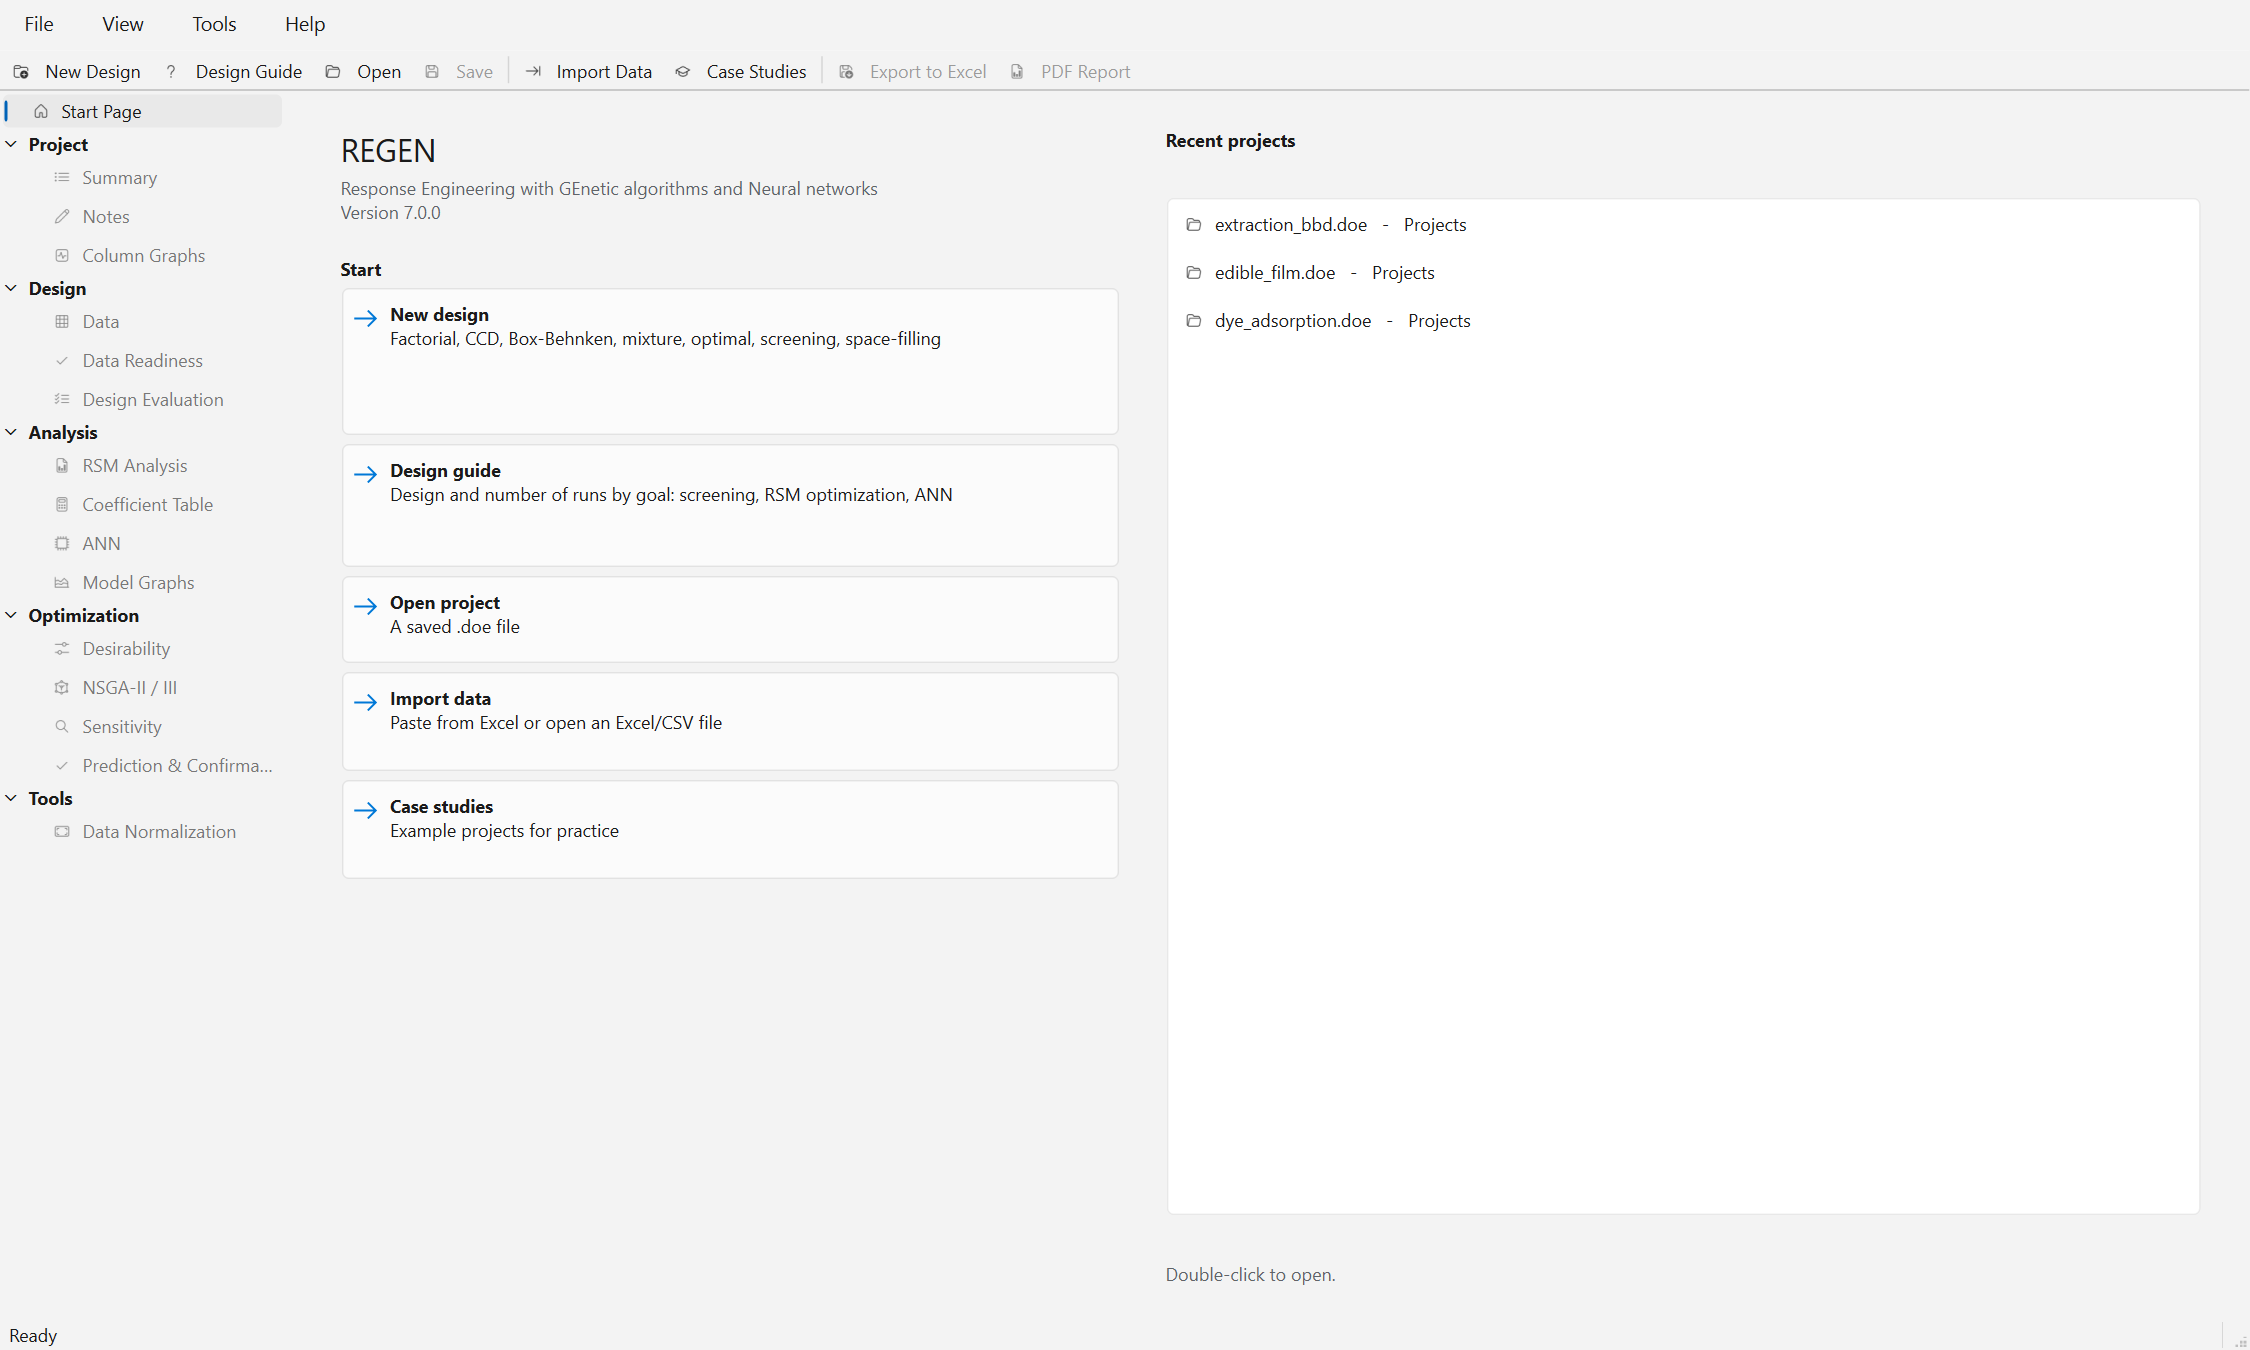
\includegraphics[width=0.85\linewidth]{start_page.png}
\caption{The main window with the Start Page. Left: navigation tree with the pages grouped by work stage. Center:
the five start buttons. Right: recent projects. Save, Export to Excel and PDF Report are greyed out because no
project is open.}
\label{fig:ch02-start}
\end{figure}

The main window (Figure~\ref{fig:ch02-start}) has a menu bar, a toolbar, the navigation tree on the left, the work
page on the right and a status bar at the bottom. The divider between the tree and the page can be dragged.

\subsection{Start Page}
The Start Page is shown when REGEN starts. Its five buttons are shortcuts to the most common first steps:
\begin{description}
  \item[\ui{New design}] ``Factorial, CCD, Box-Behnken, mixture, optimal, screening, space-filling'': opens the
        New Design dialog (Chapter~\ref{chap:3}).
  \item[\ui{Design guide}] ``Design and number of runs by goal: screening, RSM optimization, ANN'': opens the
        Design Guide (Chapter~\ref{chap:3}).
  \item[\ui{Open project}] ``A saved .doe file''.
  \item[\ui{Import data}] ``Paste from Excel or open an Excel/CSV file'' (Section~\ref{sec:ch02-import}).
  \item[\ui{Case studies}] ``Example projects for practice'' (Section~\ref{sec:ch02-cases}).
\end{description}
The list \ui{Recent projects} on the right shows the last projects that were opened or saved and still exist, as
``file name - folder''; hovering shows the full path. Double-click an entry to open it.

\subsection{Navigation tree}
\label{sec:ch02-tree}
The pages are grouped by work stage (Table~\ref{tab:ch02-pages}). All pages except the Start Page need an open
project; they are greyed out until a project is opened or created. Clicking a page refreshes it with the current
project state, so a page always shows the current models and data. The same pages can be reached from the
\ui{View} menu.

\begin{table}[htbp]
\centering
\caption{Pages of the navigation tree.}
\label{tab:ch02-pages}
\small
\begin{tabularx}{\linewidth}{@{}llX@{}}
\toprule
Group & Page & Purpose \\
\midrule
 & Start Page & Start buttons and recent projects \\
Project & Summary & Factors, responses, models and other project contents at a glance \\
 & Notes & Free-text notes (saved in the project and printed in the PDF report) \\
 & Column Graphs & Scatter plots, histograms, box plots and correlations of the raw data columns \\
Design & Data & The data sheet: runs, factor settings and responses (page title ``Data \& Design'') \\
 & Data Readiness & Scores for modeling and optimization, recommendations, suggested runs \\
 & Design Evaluation & Degrees of freedom, power, aliasing, VIF, efficiencies, FDS \\
Analysis & RSM Analysis & Model selection, ANOVA, equations, diagnostics, Box-Cox, effects, GLM, REML \\
 & Coefficient Table & Coded coefficients of all responses side by side \\
 & ANN & Artificial neural networks, architecture search, learning curve \\
 & Model Graphs & Contour, surface, effect, interaction, overlay, desirability, POE and mixture plots \\
Optimization & Desirability & Desirability optimization (page title ``Desirability Optimization'') \\
 & NSGA-II / III & Multi-objective optimization, Pareto front, checks C and D \\
 & Sensitivity & Parametric study and sensitivity analysis \\
 & Prediction \& Confirmation & Prediction, CI/PI and confirmation runs \\
Tools & Data Normalization & View and export normalized data \\
\bottomrule
\end{tabularx}
\end{table}

\subsection{Menus}
\label{sec:ch02-menus}
Table~\ref{tab:ch02-menus} lists every menu item. Items that need a project (\ui{Save}, \ui{Save As\dots},
\ui{Export to Excel\dots}, \ui{PDF Report\dots} and the pages) are disabled while no project is open.

\begin{table}[htbp]
\centering
\caption{Menu items. Shortcuts are listed in Appendix~A.}
\label{tab:ch02-menus}
\small
\begin{tabularx}{\linewidth}{@{}llX@{}}
\toprule
Menu & Item & Action \\
\midrule
File & \ui{New Design\dots} (Ctrl+N) & Create a new design (Chapter~\ref{chap:3}) \\
 & \ui{Design Guide\dots} & Choose a design and run count by goal; \ui{Create This Design\dots} fills in New
   Design \\
 & \ui{Open\dots} (Ctrl+O) & Open a project file (\texttt{*.doe}) \\
 & \ui{Open Recent} & Submenu with the recent projects (up to 8) \\
 & \ui{Import Data\dots} & Create a project from existing data (Section~\ref{sec:ch02-import}) \\
 & \ui{Case Studies\dots} & Open a built-in example (Section~\ref{sec:ch02-cases}) \\
 & \ui{Save} (Ctrl+S) & Save the project; asks for a file name the first time \\
 & \ui{Save As\dots} (Ctrl+Shift+S) & Save under a new name (\texttt{.doe} is added if missing) \\
 & \ui{Export to Excel\dots} & Data and RSM results as an Excel workbook (Section~\ref{sec:ch02-excel}) \\
 & \ui{PDF Report\dots} & Complete report as PDF (Section~\ref{sec:ch02-pdf}) \\
 & \ui{Exit} (Alt+F4) & Close REGEN (asks to save unsaved changes) \\
\addlinespace
View & one item per page & Same pages as the navigation tree, separated by group \\
\addlinespace
Tools & \ui{Data Normalization} & Opens the Data Normalization page \\
\addlinespace
Help & \ui{User Manual} (F1) & Opens this manual (PDF) \\
 & \ui{Getting Started} & Short summary of the workflow in six steps \\
 & \ui{Design Guide (RSM / ANN Run Counts)\dots} & Same as File $\rightarrow$ Design Guide \\
 & \ui{About REGEN} & Version, authors and license \\
\bottomrule
\end{tabularx}
\end{table}

Before \ui{New Design\dots}, \ui{Design Guide\dots} (when a design is created from it), \ui{Open\dots}, a recent
project, \ui{Import Data\dots}, \ui{Case Studies\dots} and when the window is closed, REGEN checks for unsaved
changes and asks ``The current project has unsaved changes. Save it first?'' with the buttons \ui{Save},
\ui{Discard} and \ui{Cancel}. If an ANN search or an NSGA run is still running when the window is closed, it is
stopped first; a running sensitivity calculation is allowed to finish.

\subsection{Toolbar}
The toolbar repeats the most used file commands: \ui{New Design}, \ui{Design Guide}, \ui{Open}, \ui{Save} $|$
\ui{Import Data}, \ui{Case Studies} $|$ \ui{Export to Excel}, \ui{PDF Report}.

\subsection{Title bar and status bar}
The window title shows the project file name followed by ``- REGEN''; ``Untitled'' is used for a project that has
not been saved yet, and an asterisk after the name means that there are unsaved changes. The right part of the
status bar shows the design description, the number of runs and the number of complete runs (runs whose responses
are all filled in), for example
\begin{quote}\small
\texttt{Box-Behnken Design (BBD) - 3 factors, 17 runs \ \ |\ \ 17 runs, 17 complete}
\end{quote}
and, if runs are excluded from the analysis, ``, $m$ excluded''. Short messages such as ``Saved: \dots'' or
``Exported to \dots'' appear on the left for a few seconds.

\section{Project files}
\label{sec:ch02-files}

A project is saved as one file with the extension \texttt{.doe} (filter ``REGEN Project (*.doe)''). The file is
plain UTF-8 text in JSON format (Appendix~A describes its structure) and contains:
\begin{itemize}
  \item the design: design type and options (including the random seed), factors with their ranges, levels and
        standard deviations, mixture total, linear constraints, blocks, whole plots and hard-to-change factors;
  \item the runs: coded factor settings, point types, run order, all response values, and the list of runs excluded
        from the analysis;
  \item the responses with their names, units, type (normal, binomial, Poisson) and number of trials;
  \item the model settings of each response (model order, selected terms, transformation) and the choice RSM or
        ANN for each response;
  \item the trained ANN models (weights, normalization and the cross-validated diagnosis), so that they do not
        have to be trained again;
  \item the optimization criteria of the Desirability page and the notes;
  \item the results of the last analyses: architecture-search results, learning curves, desirability solutions,
        the last NSGA-II/III result and the ANN vs RSM front comparison. A single result that would be very large
        (more than 5 million characters) is not saved; the project still opens without it.
\end{itemize}
RSM models are not stored as numbers but refitted from the data and the model settings when the project is opened,
so they always match the data. The sensitivity results and the confirmation values typed on the Prediction page are
not saved; they are quick to recompute.

Project files of the earlier versions named DOE Studio (versions 1 to 6) open without conversion, including older
point-type labels, and the recent-project list of those versions is kept. Files written before results were saved
simply open without stored results.

A \texttt{.doe} file can be opened by \menupath{File $\rightarrow$ Open\dots}, from \ui{Open Recent}, from the
Start Page, or by double-clicking it in Explorer when the file association was selected during installation. After
opening, the Data page is shown.

\section{Case studies}
\label{sec:ch02-cases}

\begin{figure}[htbp]
\centering
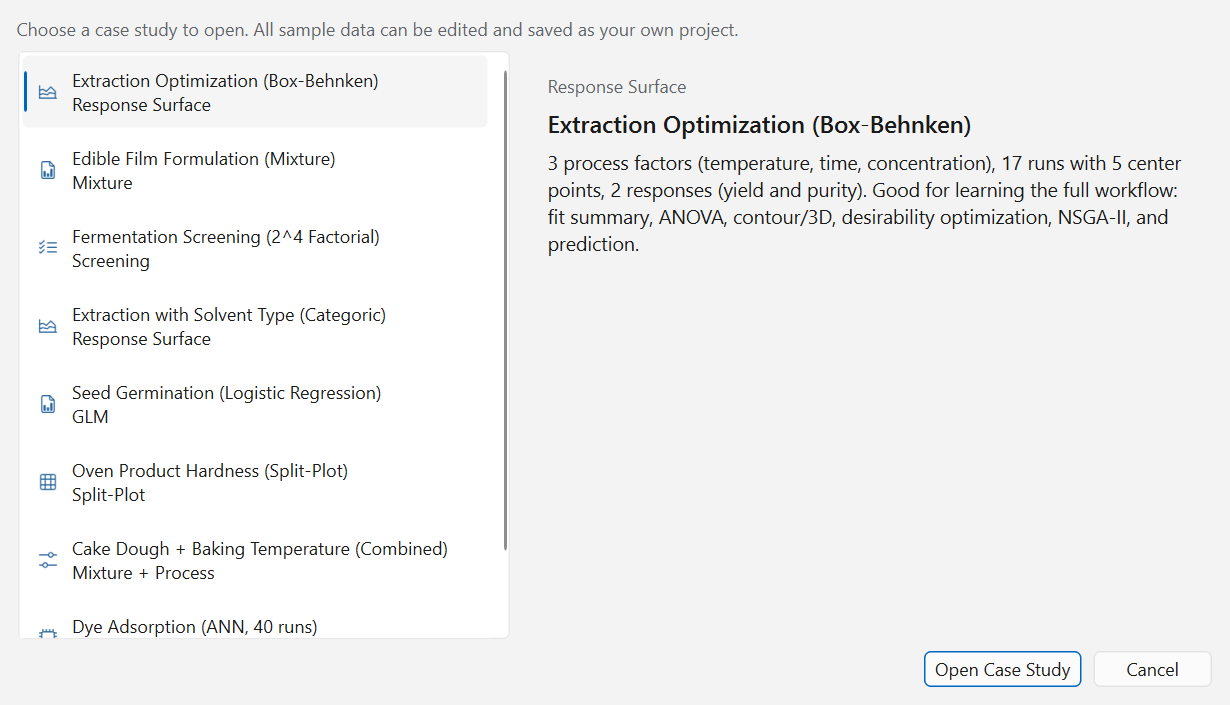
\includegraphics[width=0.65\linewidth]{case_studies.png}
\caption{The Case Studies dialog with the first case selected.}
\label{fig:ch02-cases}
\end{figure}

The eight built-in case studies (\menupath{File $\rightarrow$ Case Studies\dots}, Figure~\ref{fig:ch02-cases})
cover every analysis family of REGEN. Select a case in the list to see its description, then click \ui{Open Case
Study} (or double-click). The project opens on the Data page as an untitled project; it can be edited and saved as
your own project. The data are simulated from known equations with Gaussian noise and fixed random seeds, so every
user sees exactly the same numbers, and the ``true'' behavior is known, which makes the cases suitable for learning
and for checking the methods. Table~\ref{tab:ch02-cases} lists the cases.

\begin{table}[htbp]
\centering
\caption{Built-in case studies (in the order of the dialog).}
\label{tab:ch02-cases}
\scriptsize
\begin{tabularx}{\linewidth}{@{}p{0.17\linewidth}p{0.18\linewidth}p{0.22\linewidth}p{0.12\linewidth}X@{}}
\toprule
Case (category) & Design & Factors (range) & Responses & Good for learning \\
\midrule
Extraction Optimization (Box-Behnken) (Response Surface) &
Box-Behnken, 3 factors, 5 center points, 17 runs &
Temperature 60--80 \textdegree C; Time 30--90 min; Concentration 1--3 \% &
Yield (\%), Purity (\%) &
The whole workflow: fit summary, ANOVA, diagnostics, graphs, desirability, NSGA-II, sensitivity, prediction;
ANN vs RSM with few runs \\
\addlinespace
Edible Film Formulation (Mixture) (Mixture) &
Simplex lattice \{3,\,2\} with axial points and replicated vertices and centroid, total 100, 14 runs &
Starch $\ge$ 50 \%; Glycerol $\ge$ 10 \%; Chitosan $\ge$ 10 \% (each up to its lower limit + 30) &
Tensile Strength (MPa), Elongation (\%) &
Pseudo-components, Scheff\'e models, ternary contour, trace plot \\
\addlinespace
Fermentation Screening ($2^4$ Factorial) (Screening) &
Unreplicated two-level full factorial, 16 runs &
Temperature 30--50 \textdegree C; pH 5--7; Agitation 100--200 rpm; Inoculum 2--6 \% &
Biomass (g/L) &
Half-normal and Pareto plots of effects, Lenth's method \\
\addlinespace
Extraction with Solvent Type (Categoric) (Response Surface) &
Rotatable CCD in 2 factors with 3 center points, crossed with 3 solvents, 33 runs &
Temperature 40--60 \textdegree C; Time 2--6 h; Solvent (Ethanol, Methanol, Acetone) &
Yield (\%) &
Categoric factors, effect coding, one equation per level, optimization across levels \\
\addlinespace
Seed Germination (Logistic Regression) (GLM) &
Rotatable CCD, 2 factors, 5 center points, 13 runs &
Temperature 20--35 \textdegree C; Humidity 60--90 \% &
Germinated (seeds out of 50 per run) &
Binomial response, logistic regression, likelihood-ratio tests, odds ratios \\
\addlinespace
Oven Product Hardness (Split-Plot) (Split-Plot) &
Two-level full factorial, 2 replicates, oven temperature hard to change, 4 whole plots, 16 runs &
Oven Temperature 150--190 \textdegree C; Time 10--20 min; Concentration 1--3 \% (factor standard deviations
given) &
Hardness (N) &
Split-plot REML, variance components, whole-plot tests, propagation of error \\
\addlinespace
Cake Dough + Baking Temperature (Combined) (Mixture + Process) &
I-optimal combined design, model Quadratic $\times$ Linear, total 100, 22 runs (12 model, 5 lack of fit, 5
replicates) &
Flour 50--80 \%; Sugar 10--30 \%; Fat 10--30 \%; Temperature 160--200 \textdegree C (process) &
Texture (score) &
Combined mixture-process models, constrained mixture region \\
\addlinespace
Dye Adsorption (ANN, 40 runs) (Machine Learning) &
Historical data, 40 runs (Latin hypercube) &
pH 2--10; Adsorbent Dose 0.5--4 g/L; Contact Time 10--120 min; Initial Concentration 20--200 mg/L &
Removal Efficiency (\%) &
Strongly nonlinear data: data readiness, ANN adequacy, architecture search, learning curve, normalization, RSM vs
ANN \\
\bottomrule
\end{tabularx}
\end{table}

\section{Importing existing data}
\label{sec:ch02-import}

\paragraph{Purpose.} \ui{Import Data\dots} creates a project from data that already exist: results from earlier
experiments, plant records, a table in Excel or CSV, or a design made in another DOE program. The imported runs
become a historical-data project that can be analyzed like a designed experiment.

\begin{figure}[htbp]
\centering
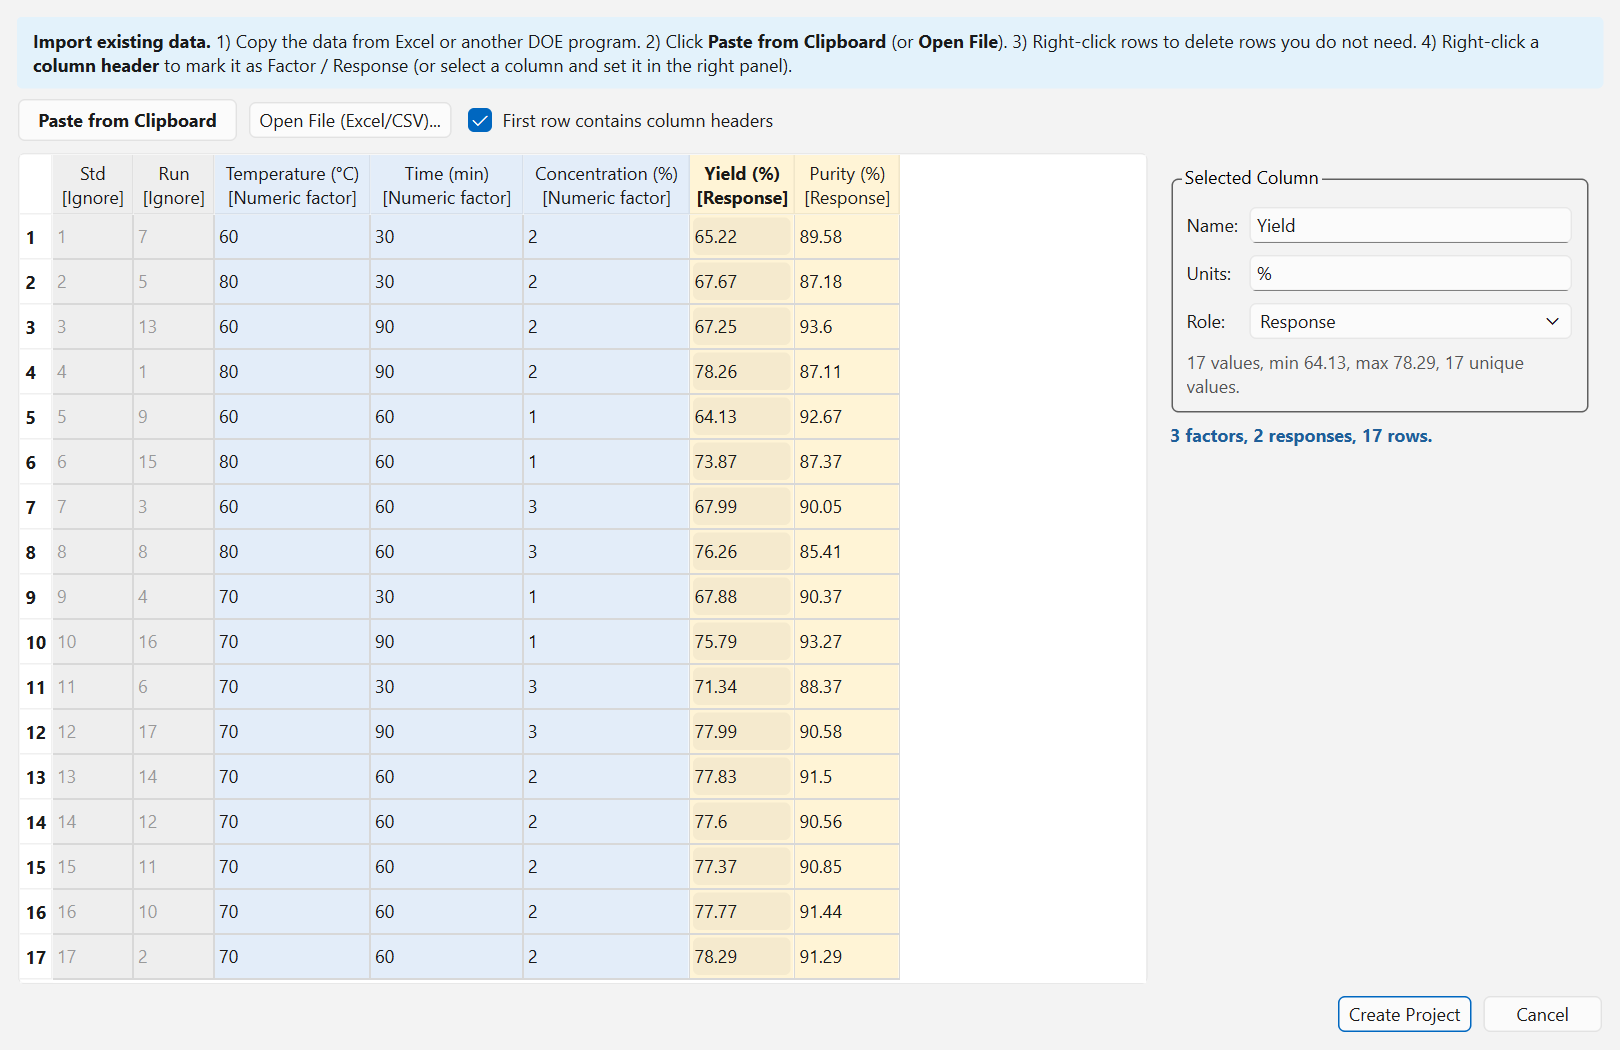
\includegraphics[width=0.8\linewidth]{import_dialog.png}
\caption{The Import Data Set dialog after pasting the 17-run Box-Behnken table. Std and Run are recognized as
bookkeeping columns (Ignore), the three factor columns as numeric factors and the two columns marked R1/R2 as
responses; names and units are taken from the headers.}
\label{fig:ch02-import}
\end{figure}

\paragraph{How to use.}
\begin{enumerate}
  \item Copy the table (with a header row if possible) in Excel or another program, then choose
        \menupath{File $\rightarrow$ Import Data\dots} and click \ui{Paste from Clipboard}. Alternatively click
        \ui{Open File (Excel/CSV)\dots} and select an \texttt{.xlsx}, \texttt{.xlsm}, \texttt{.csv} or
        \texttt{.txt} file.
  \item Check \ui{First row contains column headers}. It is set automatically when the first row contains text
        and there is more than one row.
  \item Check the role of every column. The role is shown below the column name in the header and by the column
        color. To change it, right-click the column header and choose a role, or click a column and set
        \ui{Name}, \ui{Units} and \ui{Role} in the panel \ui{Selected Column} on the right. The panel also shows the
        number of values, the minimum, maximum and number of unique values (or the levels of a categoric column).
  \item Delete rows that should not be imported: select cells in those rows, right-click and choose
        \ui{Delete $n$ Selected Rows}.
  \item For mixture data, set \ui{Mixture total} (see below).
  \item Click \ui{Create Project}. The project opens on the RSM Analysis page and is marked as unsaved.
\end{enumerate}

\paragraph{Column roles.} Table~\ref{tab:ch02-roles} lists the roles. REGEN proposes a role for every column:
\begin{itemize}
  \item a column whose header is a bookkeeping name (Std, Run, No, No., Number, Order, ID, Block, \#, and the
        Indonesian equivalents) or that is empty becomes \ui{Ignore};
  \item a column with at least 80\,\% numeric cells becomes \ui{Numeric factor}, otherwise \ui{Categoric factor};
  \item a header that starts with ``R1:'', ``R2:'', \dots{} (the style used by DOE programs) marks a
        \ui{Response}; if no column is a response, the last numeric column becomes the response.
\end{itemize}
Header prefixes ``A:'' or ``R1:'' are removed, and a unit written in parentheses or square brackets at the end of the
header (``Temperature (\textdegree C)'', ``Yield [\%]'') is moved to the \ui{Units} field. Cells that are not numbers
in a numeric, component or response column are shown in red.

\begin{table}[htbp]
\centering
\caption{Column roles in the Import Data Set dialog.}
\label{tab:ch02-roles}
\small
\begin{tabularx}{\linewidth}{@{}lX@{}}
\toprule
Role & Meaning \\
\midrule
\ui{Numeric factor} & Continuous factor. Its range (low, high) is set to the minimum and maximum of the data. \\
\ui{Categoric factor} & Factor with named levels (2 to 20 levels), in the order of first appearance. \\
\ui{Mixture component} & Component of a mixture; lower limit = data minimum, upper limit = data maximum. All
  factors must then be components (at least 2). \\
\ui{Response} & Measured response (empty cells are allowed and stay empty). \\
\ui{Ignore} & Not imported (run numbers, standard order, block labels, comments). \\
\bottomrule
\end{tabularx}
\end{table}

\paragraph{Separators and decimal marks.} Pasted Excel data are tab-separated. In text and CSV files the separator
is a semicolon when the first lines contain at least as many semicolons as commas, otherwise a comma. Numbers may use
a decimal point or a decimal comma; when both appear (``1.234,5'' or ``1,234.5'') the separator that comes last is
taken as the decimal mark. A number with only a comma, such as ``1,234'', is read as 1.234, so thousands separators
must not be used. From Excel workbooks the first worksheet is read, with the values (not the formulas) of the cells.
Completely empty rows and columns are dropped.

\paragraph{Mixture data.} When columns are marked as components, the group \ui{Mixture} appears with
\ui{Mixture total}, set automatically to the median of the row sums. If some rows do not add up to the total, REGEN
asks whether to continue (those rows are still analyzed). Mixture components cannot be combined with process
factors in an import.

\paragraph{Messages.} \ui{Create Project} checks the table and stops with a message if something is wrong, for
example ``Mark at least one Factor column and one Response column.'', ``Factor X is constant / empty - mark it as
Ignore.'', ``Column X, row 5 is not a number: 'n/a'.'' or ``X has 35 levels - should this column be numeric or
ignored?''. Chapter~\ref{chap:12} lists these messages with their remedies.

\paragraph{Result.} The design type is ``Historical Data (Process)'' or ``Historical Data (Mixture)''; the run
order is the row order and the point type of every run is ``Historical''. Factor cells of a historical project can
be edited on the Data page, and rows can be added or deleted there (Chapter~\ref{chap:4}).

\section{Exporting results}
\label{sec:ch02-export}

Every result of REGEN can leave the program, either as a complete report, as an Excel workbook, or table by table
and plot by plot.

\subsection{Export to Excel}
\label{sec:ch02-excel}
\menupath{File $\rightarrow$ Export to Excel\dots} writes a workbook (default name: the project name with
\texttt{.xlsx}):
\begin{itemize}
  \item sheet \texttt{Design}: the design description, then one row per run in run order with Std, Run, Block
        (if any), Type, Excluded (if runs are excluded), the factor settings in actual units (categoric factors as
        level names) and the responses;
  \item one sheet per response that has an RSM model (for example \texttt{R1 Yield}): transformation, ANOVA table
        (sum of squares, df, mean square, F-value, p-value), fit statistics (Std.\ Dev., Mean, C.V.\ \%, R$^2$,
        adjusted and predicted R$^2$, PRESS, Adeq Precision), coefficients in coded units (or pseudo-components)
        with standard errors, and the coefficients in actual units (one block per combination of categoric
        levels; for mixtures only when all lower limits are 0).
\end{itemize}
ANN models, optimization and sensitivity results are exported from their own pages (see below).

\subsection{PDF report}
\label{sec:ch02-pdf}
\menupath{File $\rightarrow$ PDF Report\dots} writes an A4 report and opens it. It contains, in this order:
\begin{enumerate}
  \item title, file name, date and the project notes;
  \item design summary: description, random seed, factor table, constraints and the data sheet (the first 200
        runs; the complete data are in the Excel export), with excluded runs marked;
  \item for each response: model and transformation, Fit Summary, ANOVA (or the GLM or split-plot tables), model
        equations, a diagnostics figure and a model graph;
  \item the Coefficient Table (when there is more than one response);
  \item for each response with an ANN: data adequacy, network summary and diagnosis, regression plots, RSM vs ANN,
        factor importance, network diagram and weights; learning curves if computed;
  \item Data Readiness and recommendations for each response;
  \item desirability optimization (criteria and the best solutions), if run;
  \item the NSGA-II/NSGA-III result (settings, objectives, convergence notes, Pareto front, convergence plot and the
        ten solutions with the highest TOPSIS score) and the ANN vs RSM comparison, if run.
\end{enumerate}
Results that are saved with the project (Section~\ref{sec:ch02-files}) are included also after the project is
reopened.

\subsection{Copying and exporting tables and plots}
\label{sec:ch02-copyexport}

\begin{figure}[htbp]
\centering

\includegraphics[width=\linewidth]{plot_toolbar.png}
\caption{The toolbar above every plot: Home, Back, Forward, Pan, Zoom, Subplot settings, Edit axes and Save image,
followed by \ui{Copy data} and \ui{Export data}.}
\label{fig:ch02-plottoolbar}
\end{figure}

\paragraph{Plots.} Every plot has a toolbar (Figure~\ref{fig:ch02-plottoolbar}). The first buttons reset the view,
step back and forward through zoom levels, pan, zoom to a rectangle, adjust the margins, edit axis limits, labels and
line styles, and save the image (PNG, SVG, PDF and other formats). The last two buttons export the \emph{data behind
the plot}:
\begin{description}
  \item[\ui{Copy data}] copies the data of every panel and series to the clipboard as a tab-separated table that
        can be pasted into Excel (title row, header row, values, blank row for each series);
  \item[\ui{Export data\dots}] saves the same data as an Excel workbook (one sheet per series, with the title in
        the first row and the column headers in the second) or as a CSV file (series below each other).
\end{description}
The same two commands are in the right-click menu of the plot, as \ui{Copy plot data} and \ui{Export plot
data\dots} (Figure~\ref{fig:ch02-plotmenu}); while Pan or Zoom is active the right mouse button belongs to that
tool. Lines, points, bars, histograms, error bars and heat maps are exported as drawn, with their legend names.
Contour, 3D surface, overlay, desirability and propagation-of-error plots export the full grid in actual units
with the plotted value at every grid point, and confidence bands and box plots export their underlying values, so a
plot can be redrawn exactly in another program.

\begin{figure}[htbp]
\centering
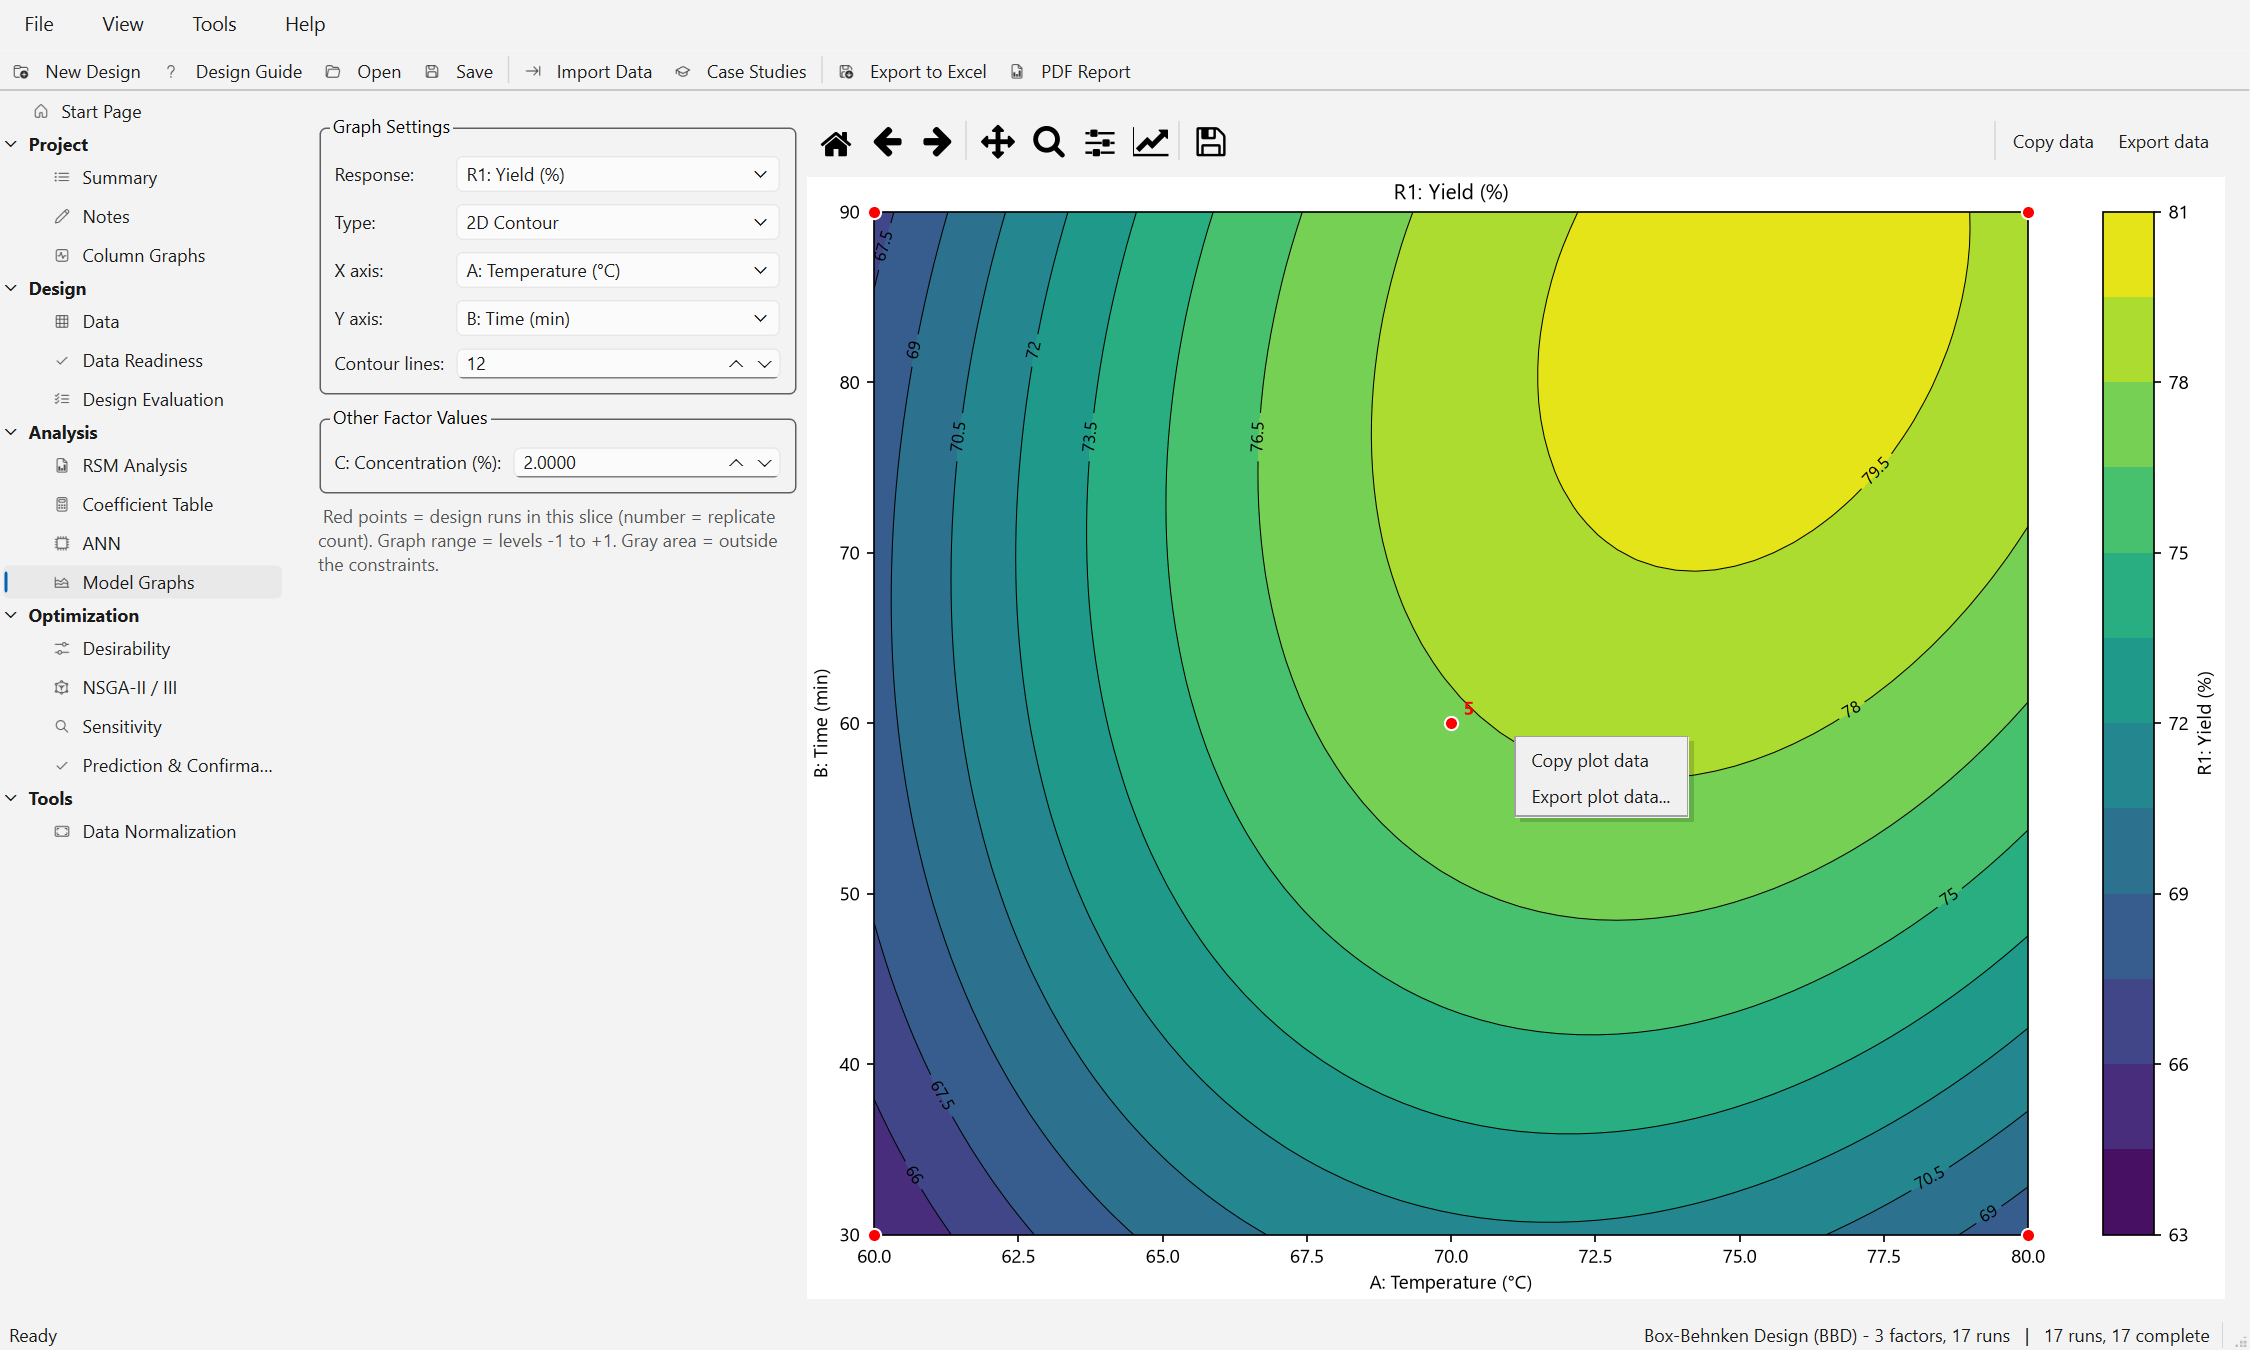
\includegraphics[width=0.5\linewidth]{plot_context_menu.png}
\caption{Right-click menu of a plot (here a contour plot).}
\label{fig:ch02-plotmenu}
\end{figure}

\paragraph{Result tables.} Every result table (solutions, Pareto solutions, diagnostics, normalized data, and so on)
has a right-click menu (Figure~\ref{fig:ch02-tablemenu}): \ui{Copy selected cells}, \ui{Copy selected cells with
column headers}, \ui{Copy entire table (for Excel)}, \ui{Copy entire table - decimal ','} (or \ui{'.'}: the
separator that is \emph{not} the Windows setting, useful when the data go to a computer with other regional
settings) and \ui{Export table\dots} (Excel or CSV; numeric cells are written as numbers). Ctrl+C copies the
selected cells.

\begin{figure}[htbp]
\centering
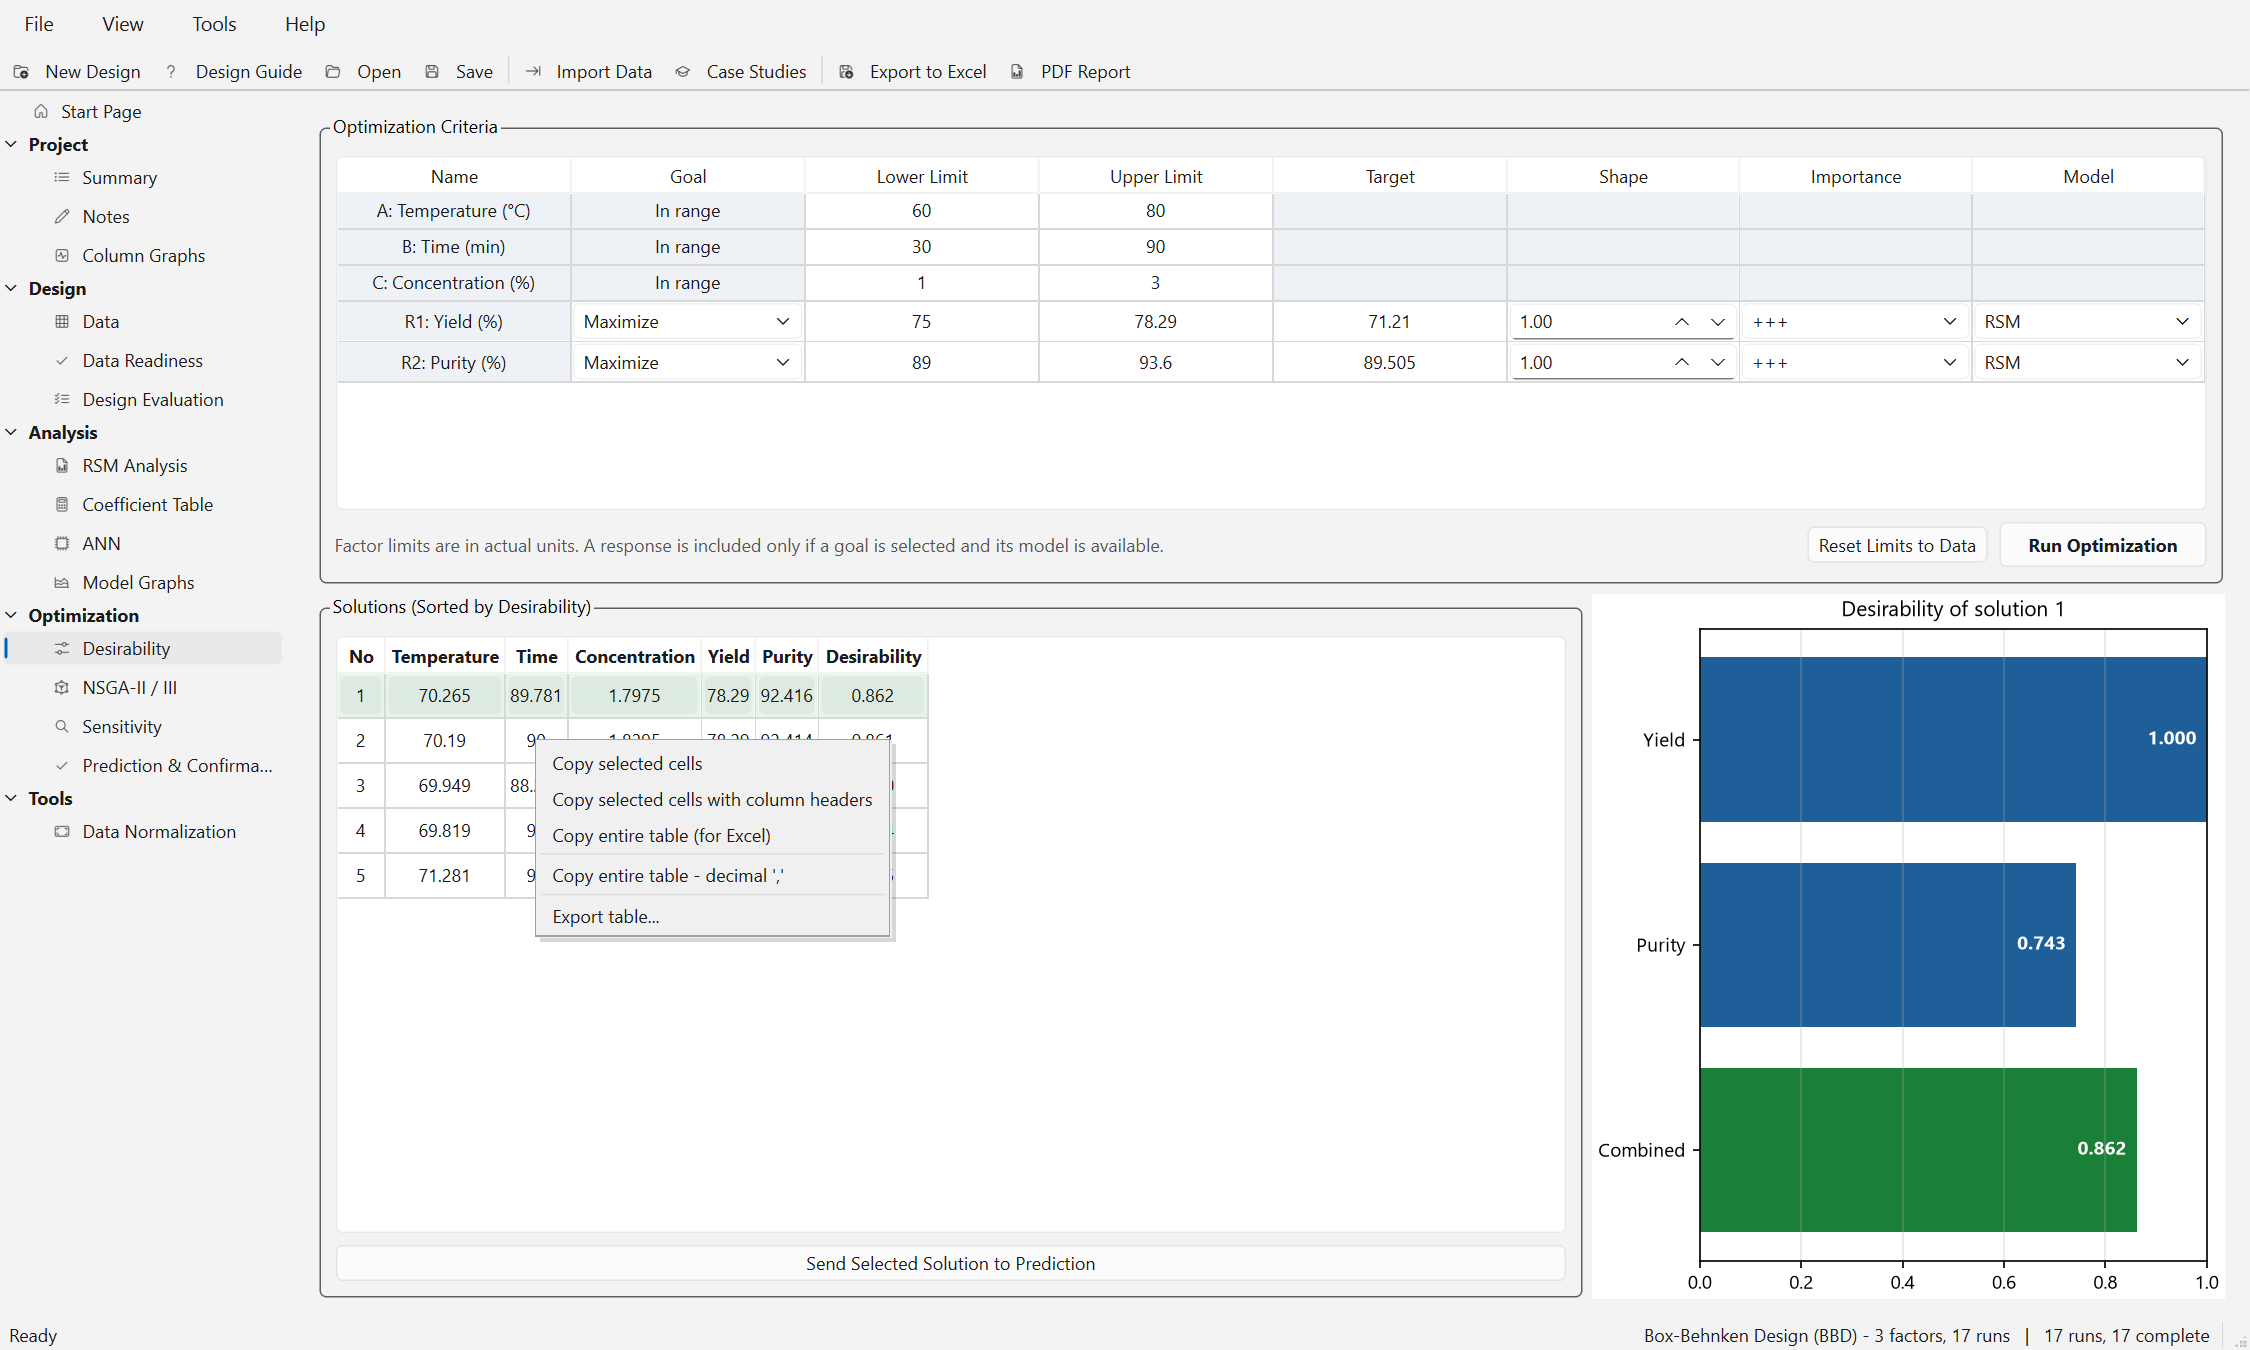
\includegraphics[width=0.5\linewidth]{table_context_menu.png}
\caption{Right-click menu of a result table (Desirability solutions).}
\label{fig:ch02-tablemenu}
\end{figure}

\paragraph{Report panels.} Text reports with tables (ANOVA, Fit Summary, Design Evaluation, Data Readiness, ANN
summary, NSGA convergence, sensitivity tables and others) have a right-click menu with the standard \ui{Copy} and
\ui{Select All} plus \ui{Copy all tables (for Excel)}, \ui{Copy all tables - decimal ','} and \ui{Export all
tables\dots}, which writes every table of the panel to its own sheet of an Excel workbook (or below each other in a
CSV file), named after the heading above the table (Figure~\ref{fig:ch02-reportmenu}).

\begin{figure}[htbp]
\centering
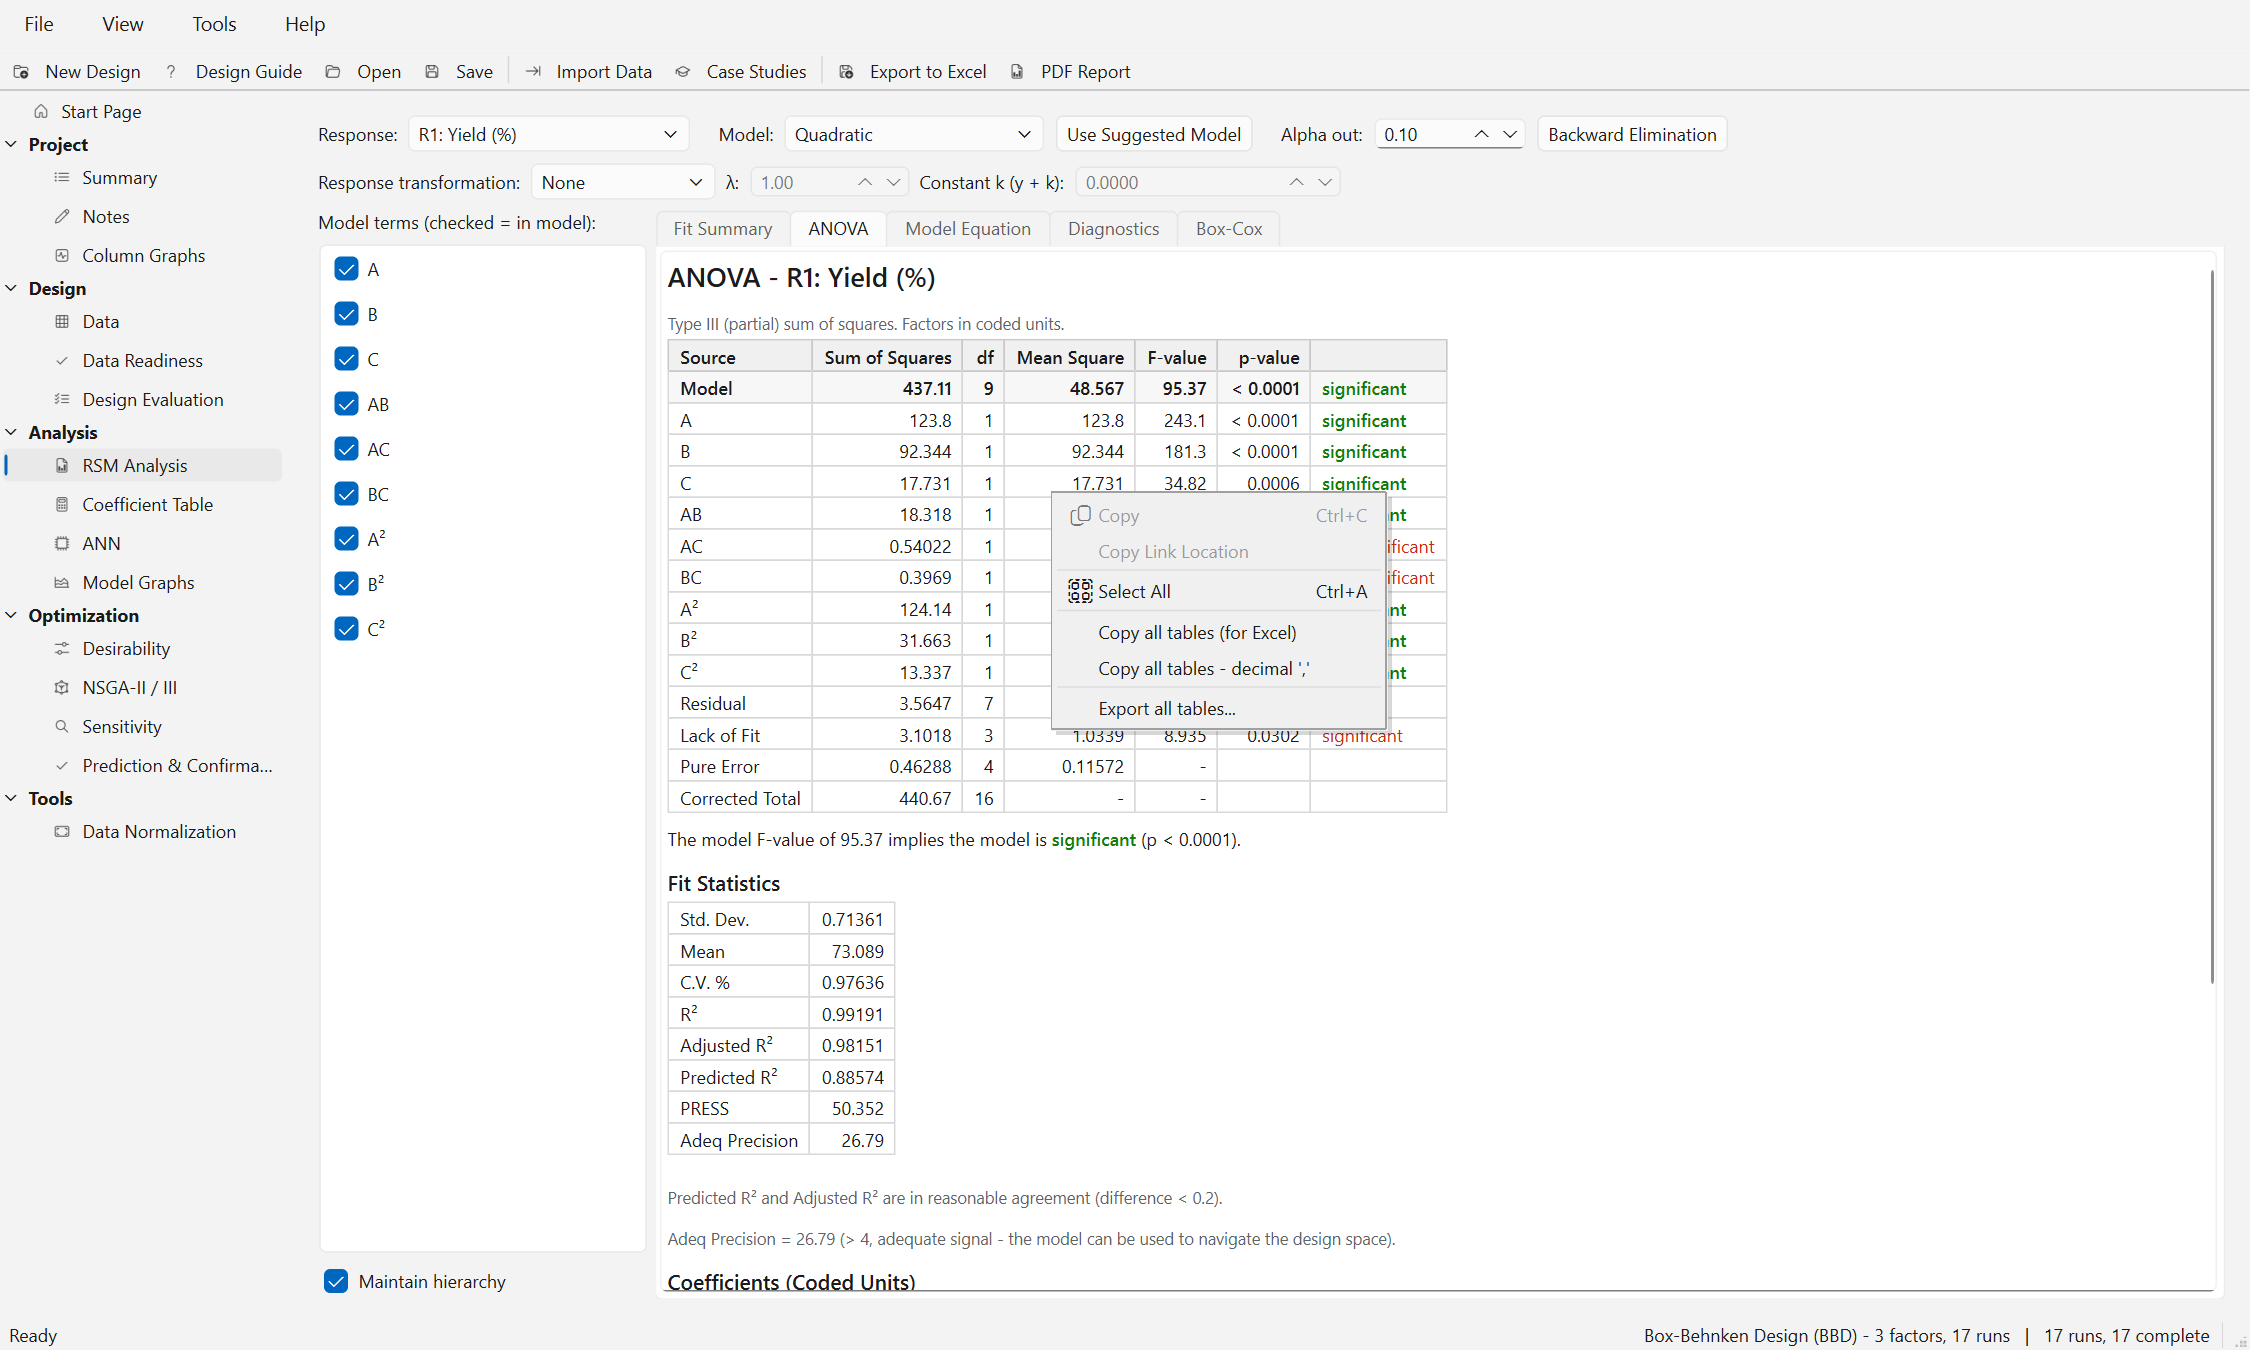
\includegraphics[width=0.5\linewidth]{report_context_menu.png}
\caption{Right-click menu of a report panel (RSM Analysis, ANOVA).}
\label{fig:ch02-reportmenu}
\end{figure}

\paragraph{Other exports.} The Data Normalization page has \ui{Export to Excel\dots} for the normalized data and
the normalization parameters, and the NSGA-II / III page has \ui{Export Pareto to Excel\dots} for the Pareto
solutions, the settings, the convergence history and the ANN vs RSM comparison (Chapter~\ref{chap:8}).

\section{Using several CPU cores}
\label{sec:ch02-cores}

ANN training, the automatic architecture search and the learning curve can run on several CPU cores. The number of
cores is set on the ANN page with \ui{CPU cores (parallel):} (shown as ``$n$ of $N$''); the default is all logical
cores minus one, so the computer stays responsive. Restarts, cross-validation folds and candidate architectures are
then computed at the same time in separate worker processes. The results are identical to those obtained with one
core, only faster; reduce the number if the computer is busy with other heavy programs or memory is short. The
worker processes are started on first use and closed automatically after 90 seconds without work.

The other computations (RSM, desirability, NSGA-II/III, sensitivity) run on one core. Long calculations run in the
background with a progress bar and a \ui{Stop} button, so the window stays responsive.

\section{A first session}
\label{sec:ch02-first}

\begin{figure}[htbp]
\centering
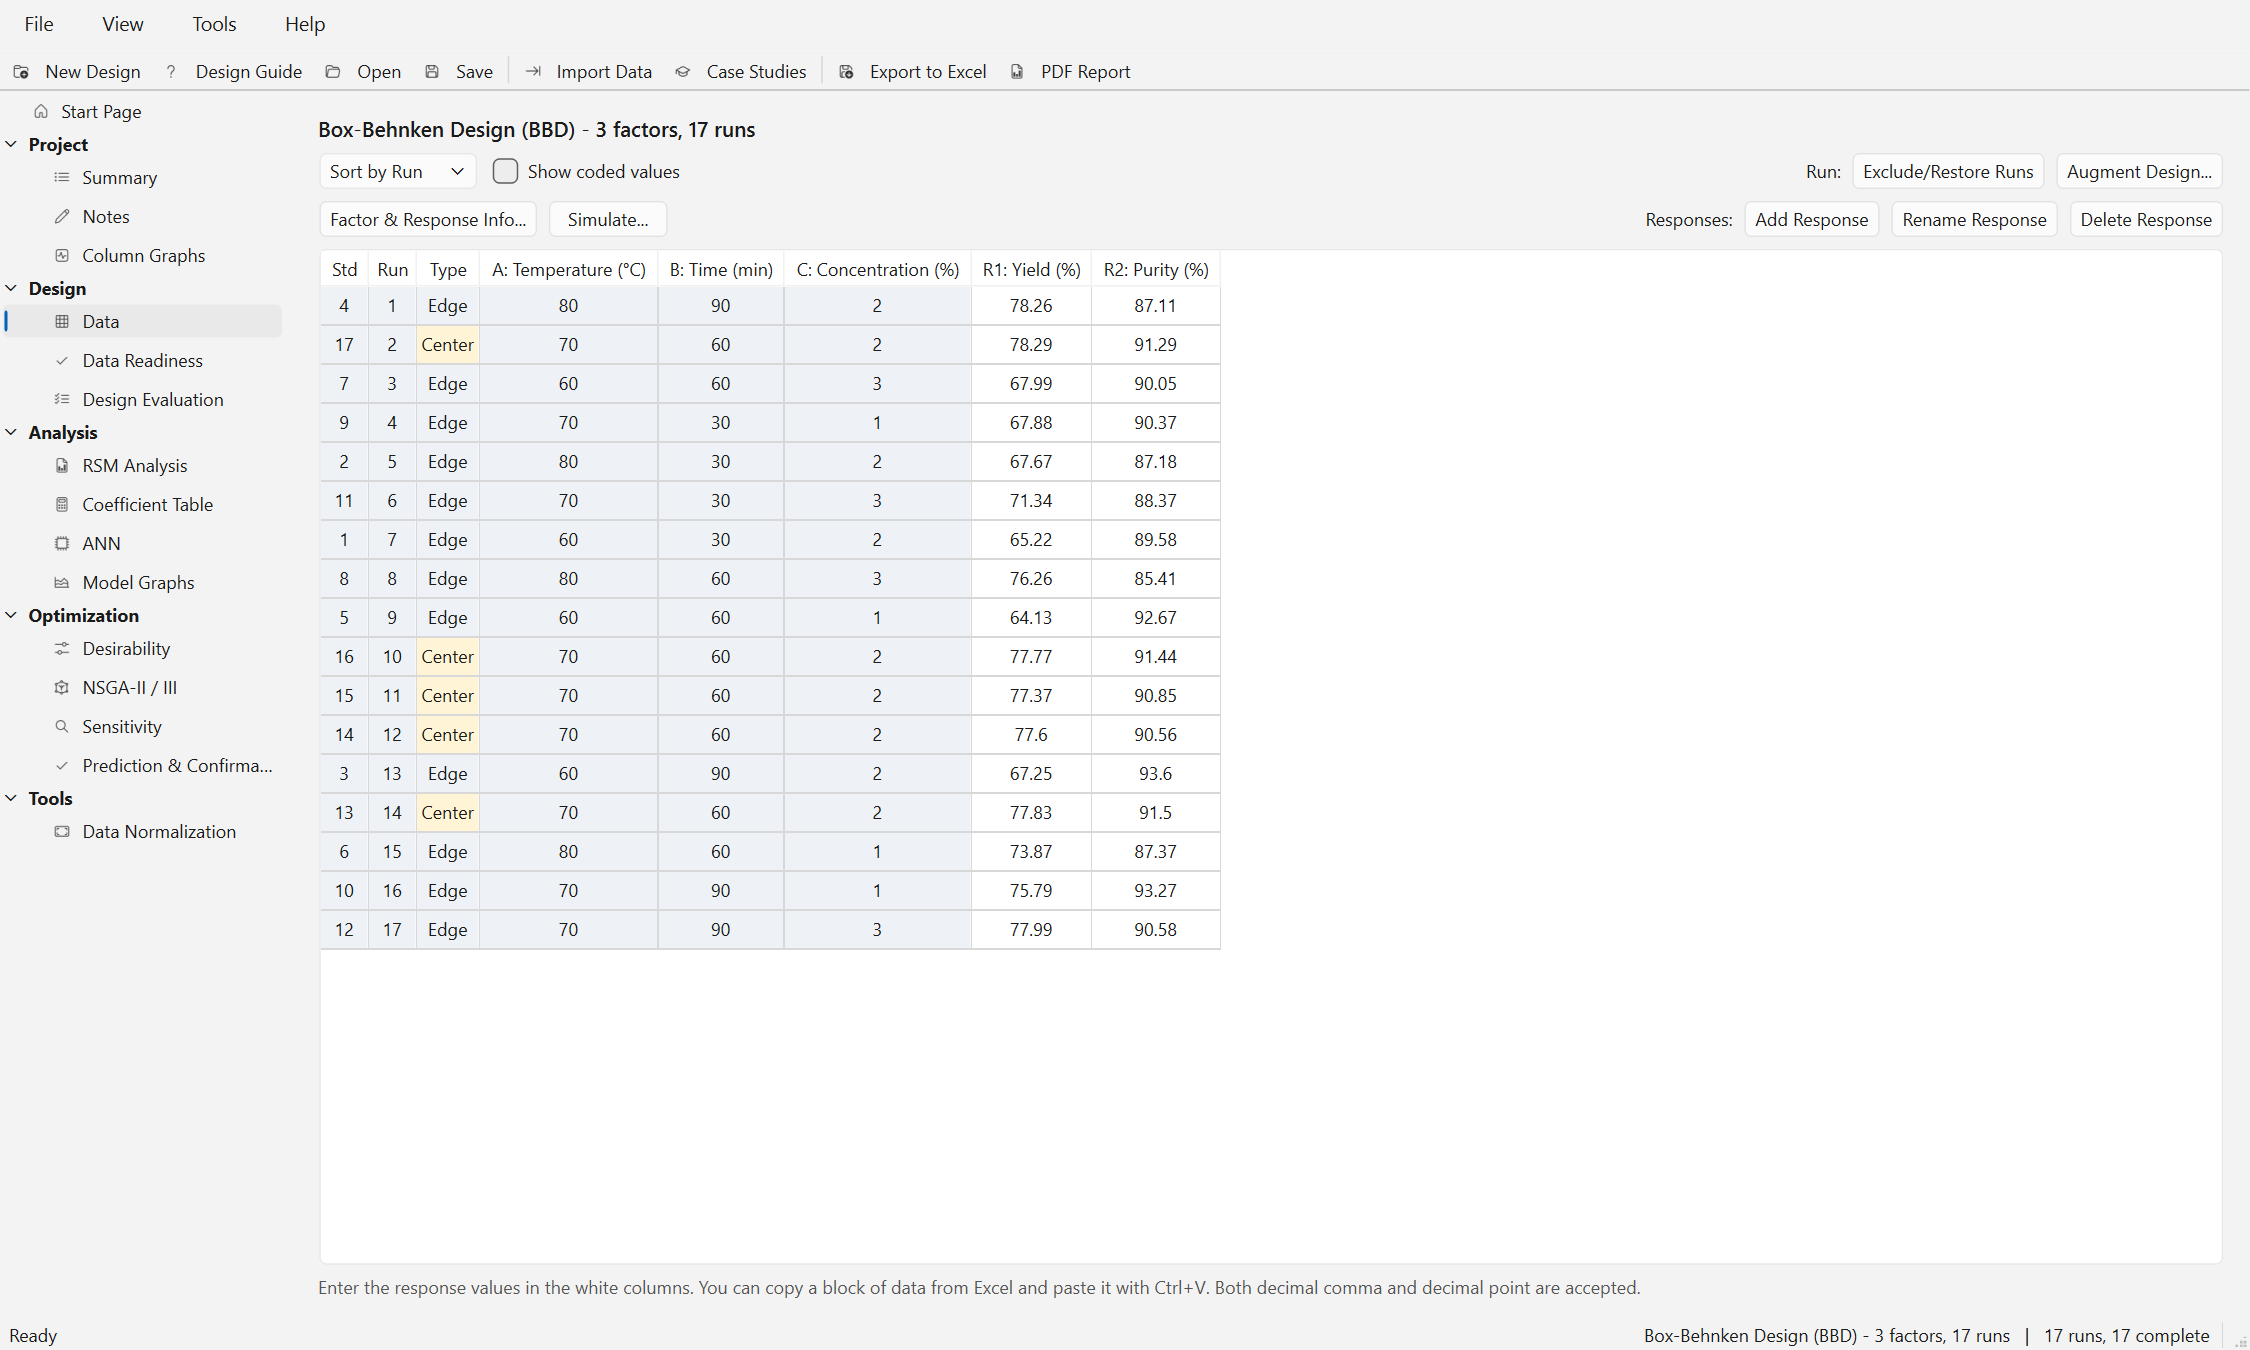
\includegraphics[width=0.8\linewidth]{data_page.png}
\caption{The Data page of the Box-Behnken extraction case study. Grey columns are factor settings (read-only in a
designed experiment), white columns are responses. The status bar shows ``17 runs, 17 complete''.}
\label{fig:ch02-data}
\end{figure}

A short tour with the first case study shows the main pages:
\begin{enumerate}
  \item Click \ui{Case studies} on the Start Page, select \ui{Extraction Optimization (Box-Behnken)} and click
        \ui{Open Case Study}. The Data page shows the 17 runs (Figure~\ref{fig:ch02-data}).
  \item Click \ui{Data Readiness}: the modeling and optimization scores of Yield are 94 and 96 (``Ready'').
  \item Click \ui{RSM Analysis}: the Fit Summary suggests the quadratic model; the ANOVA tab shows
        $R^2 = 0.9919$ and predicted $R^2 = 0.8857$ for Yield.
  \item Click \ui{Model Graphs} and choose \ui{2D Contour} or \ui{3D Surface}.
  \item On \ui{Desirability}, set the goal of Yield and Purity to \ui{Maximize} and click \ui{Run Optimization};
        then click \ui{Send Selected Solution to Prediction}.
  \item Save the project with \menupath{File $\rightarrow$ Save} and create a report with
        \menupath{File $\rightarrow$ PDF Report\dots}.
\end{enumerate}
Chapter~\ref{chap:11} continues this example in full detail.

% Chapter 3: Designing Experiments
\chapter{Designing Experiments}\label{chap:3}
\label{ch:designs}

This chapter explains how a new experiment is planned in REGEN: which design to choose for which goal, how each
design type is built, what the options in the \ui{New Design} dialog mean, how the \ui{Design Guide} recommends a
design and a number of runs, and how an existing design is extended with the \ui{Augment Design} dialog. The theory
is given as it is implemented in the program, so that the numbers shown by REGEN can be checked by hand.

\section{Choosing a design}
\label{sec:ch03-choosing}

A design is chosen by the question the experiment must answer, not by habit. REGEN distinguishes three main
situations.

\begin{description}[leftmargin=0pt]
\item[Screening.] Many factors (often six or more), little prior knowledge. The question is \emph{which factors
matter}. Main effects are enough; interactions and curvature can wait. Two-level fractional factorials of
resolution IV, Plackett--Burman designs and definitive screening designs answer this question with few runs
\citep{montgomery2017,jones2011}.
\item[Characterization and optimization (RSM).] Two to about six factors that are known to matter. The question is
\emph{how the response depends on them} and \emph{where the best setting lies}. Because an optimum inside the
region implies curvature, a second-order (quadratic) model is needed and every factor must have at least three
levels. Central composite, Box--Behnken and optimal (custom) designs are built for this purpose
\citep{box1951,box1960,myers2016}.
\item[Machine learning (ANN).] Strongly nonlinear responses (several bends, peaks, saturation) that a quadratic
polynomial cannot follow. An artificial neural network learns from examples, so it needs more runs and many levels
per factor, spread evenly over the whole region. Space-filling Latin hypercube designs and hybrid designs (a
classical RSM design plus space-filling points) serve this goal \citep{mckay1979,morris1995}.
\end{description}

Mixtures (the factors are proportions that add up to a fixed total) and experiments with hard-to-change factors
(split-plot) are special structures that can occur in all three situations; they have their own design types.
Table~\ref{tab:ch03-choice} summarizes the choice.

\begin{table}[htbp]
\centering
\caption{Which design type for which goal (k = number of numeric factors).}
\label{tab:ch03-choice}
\small
\begin{tabularx}{\linewidth}{@{}p{3.3cm}p{4.6cm}X@{}}
\toprule
Goal & Design types in REGEN & Typical run count (k = 3 unless stated) \\
\midrule
Screening & Fractional factorial (Res IV), Plackett--Burman, Definitive Screening, Taguchi array &
  k = 7: 16 + 4 center (2\textsuperscript{7-3}, Res IV), 12 (PB), 17 (DSD) \\
Ruggedness test & Fractional factorial (Res III), Plackett--Burman & k = 7: 8 (2\textsuperscript{7-4}), 12 (PB) \\
Main effects and interactions & Full factorial, fractional factorial Res V, optimal (2FI) & 8 + 4 center (2\textsuperscript{3}) \\
Optimization (RSM) & CCD, Box--Behnken, optimal (quadratic) & 20 (CCD), 17 (BBD), 20 (optimal) \\
Constrained region & Optimal (Custom) - Process with linear constraints & p + 5 + 5 \\
Formulation & Simplex lattice, simplex centroid, optimal mixture, combined mixture + process & 14 (lattice \{3,2\} with checks) \\
ANN modeling & Latin hypercube & 40 + 4 center (medium nonlinearity) \\
RSM and ANN together & Hybrid (CCD/BBD + space-filling) & 40 \\
Existing data & Historical data (or File $\rightarrow$ Import Data) & as available \\
\bottomrule
\end{tabularx}
\end{table}

\paragraph{Sequential experimentation.} It is usually cheaper to work in stages than to run one large design. A
typical path is: screen many factors with a resolution IV fraction or a DSD, keep the three or four important ones,
then run a factorial with center points; if the center points show curvature, add axial points to turn the
factorial into a central composite design (Section~\ref{sec:ch03-augment}). A definitive screening design can
already estimate curvature for the few active factors.

\paragraph{Example 1: screening seven factors.} A fermentation medium has seven candidate factors. The
\ui{Design Guide} (Section~\ref{sec:ch03-guide}) with goal \ui{Screening} and 7 factors proposes a Plackett--Burman
design with 12 runs (lowest power 74\,\% for a 2$\sigma$ effect), the fractional factorial
2\textsuperscript{7-3} of resolution IV with 4 center points (20 runs, lowest power 96\,\%) and a definitive
screening design with 17 runs (lowest power 91\,\%). The DSD is the best choice when curvature is suspected, the
2\textsuperscript{7-3} when two-factor interactions must at least be kept apart from main effects.

\paragraph{Example 2: optimizing an extraction.} Three factors (temperature, time, concentration) are known to
matter, and the best yield is expected inside the ranges. The goal \ui{RSM optimization} proposes a rotatable CCD
(20 runs, lowest power 72\,\%), a face-centered CCD (20 runs, 32\,\%), a Box--Behnken design (17 runs, 41\,\%) and
an optimal design with 20 runs. The built-in case study ``Extraction Optimization (Box-Behnken)'' uses the BBD;
Chapter~\ref{chap:4} compares these designs in detail.

\paragraph{Example 3: data for a neural network.} A dye adsorption process with four factors shows a pH optimum,
saturation with time and a Langmuir-type dependence on concentration. A quadratic model will not fit well. The goal
\ui{ANN modeling} with medium nonlinearity proposes a Latin hypercube with 65 runs plus 4 center points; the
minimum is 30 runs. The case study ``Dye Adsorption (ANN, 40 runs)'' contains 40 such runs.

\section{Factors, coding and conventions}
\label{sec:ch03-coding}

\paragraph{Factor letters.} Factors are named A, B, C, \dots{} in the order in which they are entered. The letter I
is skipped (it is reserved for the identity in defining relations), so the letters are
\texttt{ABCDEFGHJKLMNOPQRSTUVWXYZ} and at most 25 factors are possible. Numeric factors come first, then process
factors (combined designs), then categorical factors.

\paragraph{Coded units.} All designs are built and analyzed in coded units. A numeric (process) factor with low
limit $L$ and high limit $H$ is coded as
\begin{equation}
z = \frac{x - (L+H)/2}{(H-L)/2}, \qquad x = \frac{L+H}{2} + z\,\frac{H-L}{2},
\label{eq:ch03-coding}
\end{equation}
so the low level is $z=-1$, the high level $z=+1$ and the center $z=0$. Axial points of a rotatable CCD lie outside
this range ($|z| = \alpha > 1$).

\paragraph{Pseudo-components.} A mixture component $i$ with lower limit $L_i$ in a mixture with total $T$ is coded
as the pseudo-component \citep{cornell2002}
\begin{equation}
z_i = \frac{x_i - L_i}{T - \sum_j L_j}, \qquad x_i = L_i + z_i \Bigl(T - \sum_j L_j\Bigr),
\label{eq:ch03-pseudo}
\end{equation}
so that $\sum_i z_i = 1$ and $z_i \ge 0$. The quantity $T - \sum_j L_j$ is the \emph{span}: every component can
rise at most by the span above its lower limit. If an upper limit $U_i$ is given (optimal mixture and combined
designs), the effective upper limit is $H_i = \min(U_i, L_i + \text{span})$ and the coded upper bound is
$(H_i - L_i)/\text{span}$.

\paragraph{Categorical factors.} A categorical factor with $L$ levels is stored as the level index $0, \dots, L-1$
and enters models with effect coding: $L-1$ columns, where level $j<L-1$ has a 1 in column $j$ and the last level
has $-1$ in all columns. Blocks are coded the same way (sum-to-zero, $b$ blocks give $b-1$ columns). Most design
types cross the numeric design with every combination of categorical levels (Section~\ref{sec:ch03-categoric}).

\paragraph{Model orders.} The planned model is chosen from the orders available for the design: for process
designs \ui{Linear}, \ui{2FI (2-Factor Interaction)}, \ui{Quadratic} and \ui{Cubic} (two-level factorials and
Plackett--Burman: \ui{Linear}, \ui{2FI}, \ui{3FI}); for mixtures \ui{Linear}, \ui{Quadratic}, \ui{Special Cubic},
\ui{Cubic} (Scheff\'e models); for combined designs products such as \ui{Quadratic $\times$ Linear}. The number of
coefficients (including the intercept) of a process model with $k$ factors is
\begin{equation}
p_{\text{lin}} = 1+k,\quad p_{\text{2FI}} = 1 + k + \binom{k}{2},\quad
p_{\text{quad}} = \frac{(k+1)(k+2)}{2},\quad p_{\text{cubic}} = \binom{k+3}{3}.
\label{eq:ch03-ncoef}
\end{equation}
For $k = 3$ these are 4, 7, 10 and 20.

\section{The New Design dialog}
\label{sec:ch03-newdesign}

\paragraph{Purpose.} The \ui{New Design} dialog creates a new project with a design matrix, a randomized run order
and empty response columns.

\paragraph{How to use.}
\begin{enumerate}
\item Choose \menupath{File $\rightarrow$ New Design\dots} (Ctrl+N), the toolbar button \ui{New Design}, or
\ui{New design} on the Start Page. If the current project has unsaved changes, REGEN asks whether to save it first.
\item In the group \ui{Design Type}, select the \ui{Type:} and set the number of \ui{Numeric factors:} (the label
reads \ui{Components:} for mixtures and \ui{Factors:} for Taguchi arrays), \ui{Categorical factors:} (only for the
types that allow them) and \ui{Responses:} (1--20).
\item Set the options in the group \ui{Options}. Only the rows that apply to the selected type are shown.
\item Enter the names, units and limits of the factors in the factor table (Low and High for process factors;
Lower limit, and Upper limit where available, for mixture components), the level names of categorical factors
(separated by semicolons), and the names, units and types of the responses.
\item Read the blue information line at the bottom: it shows the number of runs and the main properties of the
design and is updated after every change.
\item Click \ui{Create Design}. The project opens on the \ui{Data} page. If you are unsure which design to use,
click \ui{Design Guide\dots}: the design chosen there fills in this dialog.
\end{enumerate}

\begin{figure}[htbp]
\centering
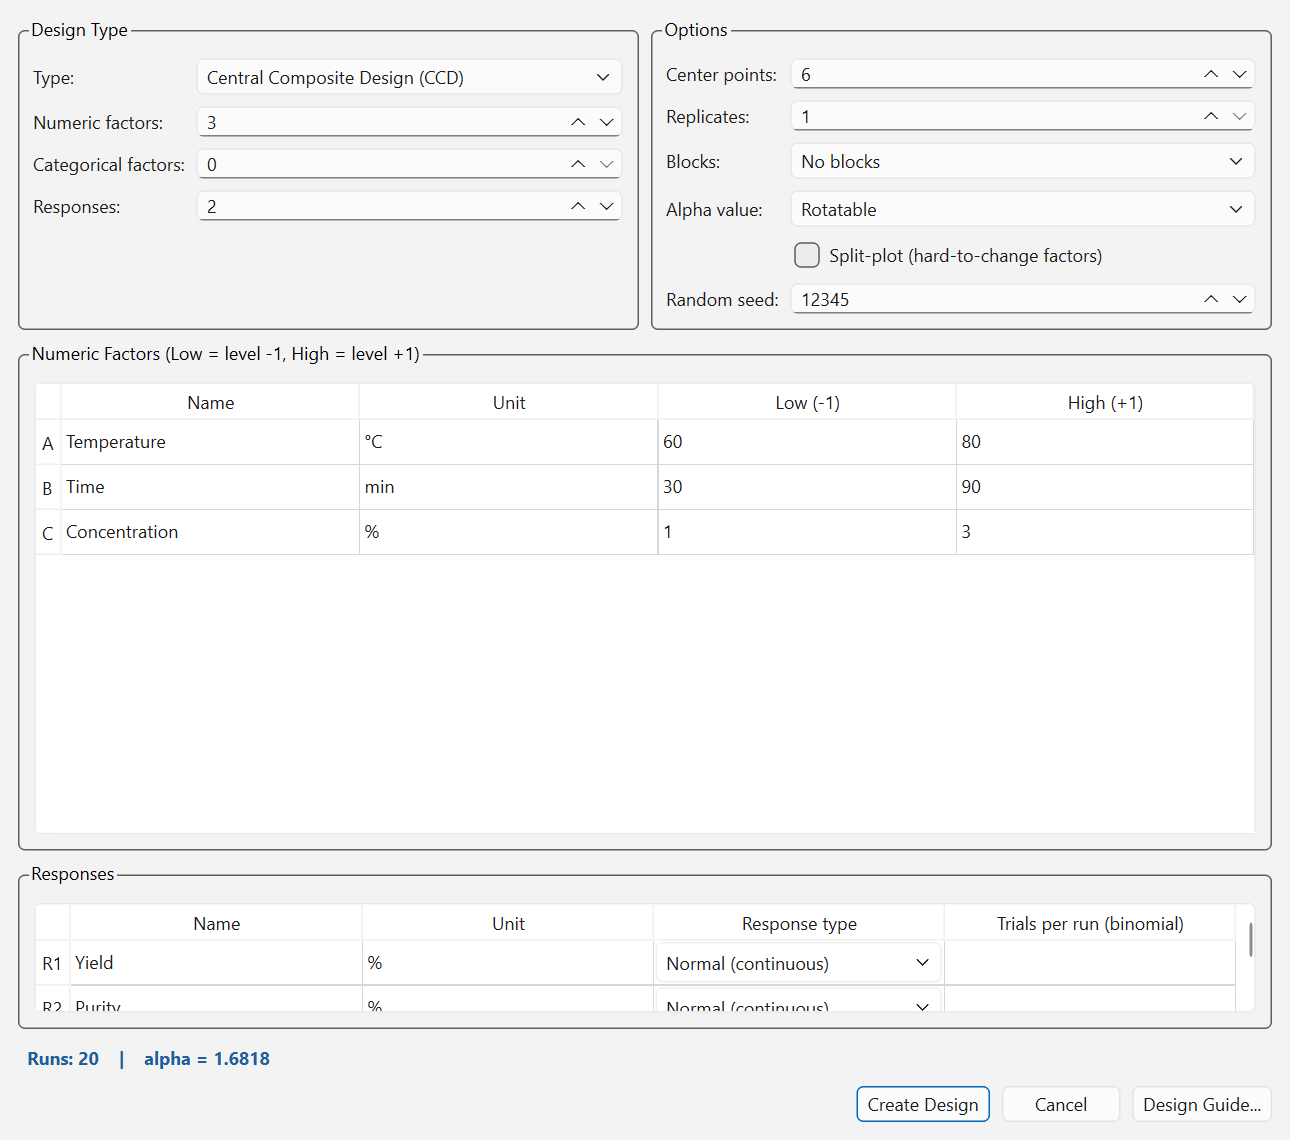
\includegraphics[width=0.75\linewidth]{new_design_ccd.png}
\caption{New Design dialog for a rotatable central composite design with three factors (Temperature 60--80
\textdegree C, Time 30--90 min, Concentration 1--3 \%), two responses and random seed 12345. The information line
reads ``Runs: 20 $|$ alpha = 1.6818''.}
\label{fig:ch03-newccd}
\end{figure}

\paragraph{Design types.} Table~\ref{tab:ch03-types} lists all types offered in the \ui{Type:} list with the
allowed number of numeric factors. The type ``Historical Data (Mixture)'' is not in the list; it is created by
\menupath{File $\rightarrow$ Import Data\dots}.

\begin{table}[htbp]
\centering
\caption{Design types of the New Design dialog.}
\label{tab:ch03-types}
\small
\begin{tabularx}{\linewidth}{@{}lcc X@{}}
\toprule
Type (as shown) & Numeric factors & Categoric & Point types created \\
\midrule
2-Level Full Factorial & 1--9 & yes & Factorial, Center \\
2-Level Fractional Factorial & 3--21 & no & Factorial, Center \\
General Factorial (Multilevel Categoric) & 0 (1--4 categoric) & required & Factorial \\
Central Composite Design (CCD) & 2--6 & yes & Factorial, Axial, Center \\
Box-Behnken Design (BBD) & 3--7 & yes & Edge, Center \\
Optimal (Custom) - Process & 1--8 & yes & Model, Lack of Fit, Replicate \\
Historical Data (Process) & 1--10 & yes & Historical \\
Screening: Plackett-Burman & 2--23 & no & Screening, Center \\
Screening: Definitive Screening Design (DSD) & 3--20 & no & Screening \\
Screening: Taguchi Orthogonal Array & 2--15 & no & Orthogonal \\
Mixture: Simplex Lattice & 3--6 & no & Vertex, Edge, Interior, Axial, Centroid \\
Mixture: Simplex Centroid & 3--6 & no & Vertex, Edge, Interior, Axial, Centroid \\
Mixture: Optimal (Custom) & 2--8 & no & Model, Lack of Fit, Replicate \\
Combined Mixture + Process (Optimal) & 2--6 comp.\ + 1--4 process & no & Model, Lack of Fit, Replicate \\
Space-filling: Latin Hypercube (for ANN) & 1--20 & yes & Space-filling, Center \\
Hybrid RSM + Space-filling (for RSM \& ANN) & 2--7 & yes & base types, Space-filling, Center \\
\bottomrule
\end{tabularx}
\end{table}

\paragraph{Options.} Table~\ref{tab:ch03-options} lists every option row of the dialog.

\begin{longtable}{@{}p{3.4cm}p{3.6cm}p{2.6cm}p{5.0cm}@{}}
\caption{Options of the New Design dialog.}\label{tab:ch03-options}\\
\toprule
Option & Values & Default & Shown for / meaning \\
\midrule
\endfirsthead
\toprule
Option & Values & Default & Shown for / meaning \\
\midrule
\endhead
\ui{Center points:} & 0--50 & CCD: 5, 6, 6, 6, 9 for k = 2--6; BBD: 5, 5, 6, 6, 6 for k = 3--7; LHS and hybrid: 4; others 0 &
  Full and fractional factorial, CCD, BBD, Plackett--Burman, LHS, hybrid. Reset when k or the type changes. \\
\ui{Replicates:} & 1--10 & 1 & Factorials, CCD, BBD, general factorial. Repeats the whole design except the center points. \\
\ui{Blocks:} & No blocks, 2, 3, 4, 8 blocks & No blocks & Only shown when blocking is possible (Section~\ref{sec:ch03-blocks}). \\
\ui{Fraction:} & ``2\textasciicircum(k-p) = N runs, Resolution R'' & smallest p & Fractional factorial. \\
\ui{Alpha value:} & Rotatable, Face-centered (alpha = 1), Orthogonal, Custom & Rotatable & CCD. \\
\ui{Custom alpha:} & 0.1--5 & 1.5 & CCD with Custom alpha. \\
\ui{Lattice degree (m):} & 1--4 & 2 & Simplex lattice. \\
\ui{Mixture total:} & 0.0001--10\textsuperscript{9} & 100 & Mixture types. \\
\ui{Add axial points + centroid} & check box & on & Simplex lattice and centroid. \\
\ui{Replicate vertices + centroid} & check box & on & Simplex lattice and centroid. \\
\ui{Criterion:} & I-optimal (best prediction), D-optimal (best coefficients) & I-optimal & Optimal types. \\
\ui{Planned model:} & orders of the design & Quadratic (combined: Quadratic $\times$ Linear) & Optimal types. \\
\ui{Additional model points:} & 0--50 & 0 & Optimal types: points chosen by the criterion beyond the p required. \\
\ui{Lack of fit points:} & 0--30 & 5 & Optimal types. \\
\ui{Replicate points:} & 0--30 & 5 & Optimal types. \\
\ui{Data rows:} & 1--5000 & 20 & Historical data: number of empty rows. \\
\ui{Plackett-Burman size:} & 12, 20, 24 runs & 12 runs & Plackett--Burman. \\
\ui{Orthogonal array:} & L4, L8, L9, L12, L16, L18, L27 & L8 (2\textasciicircum 7) & Taguchi. \\
\ui{Process factors:} & 1--4 & 1 & Combined mixture + process. \\
\ui{Split-plot (hard-to-change factors)} & check box & off & Full factorial, general factorial, CCD, BBD, optimal process. \\
\ui{Hard-to-change factors:} & factor letters, e.g.\ ``A'' or ``A, C'' & A & Split-plot. \\
\ui{Runs per whole plot:} & 0--100 (0 = automatic) & automatic & Split-plot. \\
\ui{Latin Hypercube points:} & 4--5000 & ANN target for k (k = 3: 40) & Latin hypercube; each factor gets this many levels. \\
\ui{Base design:} & CCD face-centered (3 level), CCD rotatable (5 level), Box-Behnken (3 level), Factorial (2 level) & CCD face-centered & Hybrid. \\
\ui{Space-filling points:} & 0--5000 & 12 & Hybrid. \\
\ui{Random seed:} & 1--999\,999\,999 & random number drawn when the dialog opens & All types (Section~\ref{sec:ch03-random}). \\
\bottomrule
\end{longtable}

\paragraph{Information line.} The line at the bottom of the dialog shows, depending on the type: ``Runs: N'' and
the generators of a fraction (``generator: E = ABCD, \dots''), the alpha of a CCD (``alpha = 1.6818''), the number
of blocks, the categorical crossing (``(11 $\times$ 3 categorical level combinations)''), the hard-to-change factors,
the span of a mixture (``Each component can rise up to its lower limit + 30'') or the coefficient count of an
optimal design (``Model Quadratic: 14 coefficients $\rightarrow$ 24 runs in total (14 model + 5 lack of fit + 5
replicates)''). For Latin hypercube and hybrid designs it adds a verdict on the run count for an ANN
(Section~\ref{sec:ch03-guide-calc}). A text beginning with ``Invalid:'' means the current settings cannot be built;
for example ``Invalid: PB with 12 runs allows at most 11 factors.''

\paragraph{Messages on Create Design.} Invalid inputs are reported in a message box titled ``Invalid Input'': ``The
limits of \textless name\textgreater{} are not numbers.'', ``Factor \textless name\textgreater: Low must be less
than High.'', ``The lower limit of \textless name\textgreater{} cannot be negative.'', ``The upper limit of
\textless name\textgreater{} must be greater than the lower limit.'', ``Categorical factor \textless
name\textgreater{} needs at least 2 distinct levels.'', ``The sum of the component lower limits must be less than
the total.'' and ``Response \textless i\textgreater: enter the number of trials per run ($\ge$ 1).'' (binomial
responses). Constraint errors are shown under ``Constraint'' (Section~\ref{sec:ch03-constraints}); a split-plot
without hard-to-change letters gives ``Enter the letters of the hard-to-change factors (e.g. A).''. If the
generator itself fails, the title is ``Design Could Not Be Created'', for example ``There are not enough candidate
points to estimate this model. Relax the constraints or choose a simpler model.''

\section{Two-level factorial designs}
\label{sec:ch03-factorial}

\subsection{Full factorial}
The 2\textsuperscript{k} full factorial contains every combination of the low and high levels of $k$ factors, in
standard (Yates) order with factor A changing fastest \citep{montgomery2017}. All main effects and all interactions
are estimable and orthogonal. Replicates repeat the whole set; center points are added once at the end. Center
points do not change the estimates of the factorial effects but provide pure error and a test for curvature. The
run count doubles with every factor, which limits the type to $k \le 9$ (512 runs).

\subsection{Blocking}
\label{sec:ch03-blocks}
When the runs cannot all be performed under the same conditions (several days, batches of raw material), the design
is divided into blocks and a block effect is included in the model. For a full factorial REGEN confounds selected
high-order interactions with blocks, using the generators in Table~\ref{tab:ch03-blockgen}
\citep{montgomery2017}. The block of a run is coded from the signs of the generator products,
\begin{equation}
b = \sum_{j} \Bigl[\,\textstyle\prod_{c \in w_j} z_c > 0\Bigr]\, 2^{\,j},
\label{eq:ch03-blocklabel}
\end{equation}
and the labels are renumbered in order of first appearance so that block 1 contains standard run 1. The generators
and all their products are confounded with blocks and cannot be estimated. Center points are spread evenly over the
blocks. The run order is randomized within each block, and the blocks are run in sequence.

\begin{table}[htbp]
\centering
\caption{Block generators of the 2\textsuperscript{k} full factorial.}
\label{tab:ch03-blockgen}
\small
\begin{tabular}{@{}cccc@{}}
\toprule
k & 2 blocks & 4 blocks & 8 blocks \\
\midrule
2 & AB & -- & -- \\
3 & ABC & AB, AC & -- \\
4 & ABCD & ABC, ACD & AB, BC, CD \\
5 & ABCDE & ABC, CDE & ABE, BCE, CDE \\
6 & ABCDEF & ABCF, CDEF & ABEF, ABCD, ACE \\
7 & ABCDEFG & ABCFG, CDEFG & ABC, DEF, AFG \\
\bottomrule
\end{tabular}
\end{table}

For a 2\textsuperscript{3} in two blocks with two center points, the generator ABC puts the runs with $ABC = -1$
(standard runs 1, 4, 6, 7) and one center point into block 1 and the other four runs and the second center point into
block 2. CCDs and the four-factor BBD have their own blocking rules (Sections~\ref{sec:ch03-ccd} and
\ref{sec:ch03-bbd}); other design types are not blocked when created, but augmentation can add runs as a new block.

\subsection{Fractional factorial}
\label{sec:ch03-fraction}
A 2\textsuperscript{k-p} fractional factorial uses $2^{k-p}$ runs. The first $k-p$ factors form a full factorial
(the base design); each of the $p$ added factors is set equal to the product of a group of base factors, its
\emph{generator}. For example, the 2\textsuperscript{6-2} uses E = ABC and F = BCD.

\paragraph{Defining relation.} Each generator gives a defining word $w_i = g_i \cup \{\text{new letter}\}$ (E = ABC
gives the word ABCE). The defining relation consists of the $2^p - 1$ words generated by all products of the
generator words, where letters that appear twice cancel (symmetric difference). For the 2\textsuperscript{6-2},
I = ABCE = BCDF = ADEF.

\paragraph{Word length pattern and resolution.} The word length pattern is $(A_1, A_2, \dots, A_k)$, where $A_j$
is the number of words of length $j$. The resolution is the length of the shortest word,
\begin{equation}
R = \min\{\, j : A_j > 0 \,\}.
\label{eq:ch03-resolution}
\end{equation}
In a resolution III design main effects are aliased with two-factor interactions; in resolution IV main effects are
free of two-factor interactions, but two-factor interactions are aliased with each other; in resolution V main
effects and two-factor interactions are aliased only with three-factor and higher interactions
\citep{montgomery2017}. REGEN shows the resolution in Roman numerals.

\paragraph{Aliases.} The alias of an effect $e$ with respect to the word $w$ is $e \oplus w$ (the letters in exactly
one of the two). REGEN lists the aliases of all main effects and two-factor interactions that have at most three
letters. In the 2\textsuperscript{5-2} with D = AB and E = AC (I = ABD = ACE = BCDE, word length pattern $A_3 = 2$,
$A_4 = 1$), the main effect A is aliased with BD and CE, so the design has resolution III.

\paragraph{Minimum aberration.} Different generator choices with the same resolution are not equally good. The
preferred fraction has the fewest words of the shortest length: it minimizes $A_R$, then $A_{R+1}$, and so on
\citep{fries1980}. For up to seven factors REGEN uses the textbook generators (for example 2\textsuperscript{7-3}:
E = ABC, F = BCD, G = ACD). For 8--21 factors the generators were found by computer search: maximum resolution
first, then minimum aberration; the resolution of each cell matches the standard two-level factorial table. Runs
from 4 to 512 are available.

\paragraph{Example: 2\textsuperscript{7-3}.} With generators E = ABC, F = BCD, G = ACD the defining relation has
seven words, all of length four: I = ABCE = ABFG = ACDG = ADEF = BCDF = BDEG = CEFG. The word length pattern is
$A_4 = 7$, so the resolution is IV. The main effect A is aliased only with three-factor interactions (BCE, DEF,
CDG, BFG), while AB = CE = FG. The \ui{Fraction:} list for seven factors offers 2\textsuperscript{7-1} (64 runs,
Res VII), 2\textsuperscript{7-2} (32 runs, Res IV), 2\textsuperscript{7-3} (16 runs, Res IV) and
2\textsuperscript{7-4} (8 runs, Res III).

\subsection{General factorial}
The type ``General Factorial (Multilevel Categoric)'' contains every combination of the levels of 1--4 categorical
factors (no numeric factors), repeated \ui{Replicates:} times. It is used when all factors are categorical with two
or more levels, for example three catalysts $\times$ two solvents.

\section{Screening designs}
\label{sec:ch03-screening}

\subsection{Plackett--Burman}
Plackett--Burman designs \citep{plackett1946} are two-level orthogonal arrays whose run count is a multiple of four.
REGEN builds them from the cyclic generator rows
\begin{center}\small
\begin{tabular}{@{}rl@{}}
12 runs: & \texttt{++-+++---+-}\\
20 runs: & \texttt{++--++++-+-+----++-}\\
24 runs: & \texttt{+++++-+-++--++--+-+----}
\end{tabular}
\end{center}
The design consists of the $N-1$ cyclic shifts of the generator row plus a row of all minus signs; the first $k$
columns are used ($k \le N-1$). The columns are orthogonal: $X^\top X = N I$. Main effects are partially aliased
with many two-factor interactions (each interaction is spread over several main-effect columns with coefficients
$\pm 1/3$ in the 12-run design), so these designs assume that interactions are small. Center points can be added to
detect curvature. The model is linear; the Effects plots of the analysis show main effects only.

\subsection{Definitive screening designs}
A definitive screening design \citep{jones2011} has three levels and $2m+1$ runs:
\begin{equation}
D = \begin{bmatrix} C \\ -C \\ \mathbf{0}^\top \end{bmatrix},
\label{eq:ch03-dsd}
\end{equation}
where $C$ is an $m \times m$ conference matrix: zero diagonal, $\pm 1$ elsewhere, and $C C^\top = (m-1) I$
\citep{xiao2012}. Each pair of runs $(c, -c)$ is a fold-over pair, so main effects are not aliased with any
two-factor interaction or quadratic effect, and quadratic effects are estimable. REGEN uses $m = k$ for even $k$
and $m = k+1$ for odd $k$ (the extra column is dropped), rounded up to an available order
$m \in \{4, 6, 8, 10, 12, 14, 18, 20\}$. The conference matrix is built with the Paley construction
\citep{paley1933} from the finite field with $q = m-1$ elements ($q \in \{3, 5, 7, 9, 11, 13, 17, 19\}$; GF(9) is
represented as $a + b\,i$ with $i^2 = -1 \bmod 3$): first row $(0, 1, \dots, 1)$, first column $\chi(-1)$ and
$C_{ij} = \chi(e_j - e_i)$, with $\chi$ the quadratic character of the field. The design contains one center run;
there is no option for more. Table~\ref{tab:ch03-dsd} lists the run counts. Because no Paley matrix of order 16 is
available, 15 and 16 factors use the order-18 matrix (37 runs).

\begin{table}[htbp]
\centering
\caption{Runs of the definitive screening design.}
\label{tab:ch03-dsd}
\small
\begin{tabular}{@{}lcccccccccc@{}}
\toprule
k & 3--4 & 5--6 & 7--8 & 9--10 & 11--12 & 13--14 & 15--18 & 19--20 \\
Runs & 9 & 13 & 17 & 21 & 25 & 29 & 37 & 41 \\
\bottomrule
\end{tabular}
\end{table}

A DSD estimates all main effects with high precision; a full quadratic model is estimable only when few factors
turn out to be active. With three factors, 9 runs cannot support the 10 coefficients of a full quadratic model:
Design Evaluation then reports aliased terms and only 1 residual degree of freedom. REGEN therefore uses the
\ui{Linear} model as the default for a DSD (on the Design Evaluation and RSM Analysis pages); add
two-factor interactions or squared terms only for the few factors that turn out to be active.

\subsection{Taguchi orthogonal arrays}
The arrays L4 (2\textsuperscript{3}), L8 (2\textsuperscript{7}), L16 (2\textsuperscript{15}) consist of all
interaction columns of a 2-, 3- and 4-factor full factorial (column 1 changes slowest); L9 (3\textsuperscript{4})
and L27 (3\textsuperscript{13}) are built from linear combinations over GF(3) with levels $-1, 0, +1$; L12 is the
12-run Plackett--Burman design; L18 (2\textsuperscript{1} $\times$ 3\textsuperscript{7}) is the standard table
with a two-level first column and seven three-level columns. The first $k$ columns are used. The information line
lists the levels of each factor. The signs of some interaction columns differ from printed tables; this is only a
relabelling of the levels and does not affect orthogonality. Taguchi arrays have no center points, replicates or
blocks. They are useful for screening many factors with few runs; for the analysis REGEN uses the same regression
models as for other designs, with the \ui{Linear} model as the default (signal-to-noise ratios in the Taguchi sense
are not computed).

\section{Response surface designs}
\label{sec:ch03-rsm}

\subsection{Central composite design}
\label{sec:ch03-ccd}
The CCD \citep{box1951} combines three parts: the $n_F = 2^k$ factorial points (type ``Factorial''), $2k$ axial
points at $\pm\alpha$ on each axis (type ``Axial'') and $n_C$ center points. Replicates repeat the factorial and
axial points; the center points are added once. The axial distance $\alpha$ is set by \ui{Alpha value:}
\citep{myers2016,montgomery2017}:
\begin{align}
\text{Rotatable:}\quad & \alpha = n_F^{1/4}, \label{eq:ch03-alpharot}\\
\text{Face-centered:}\quad & \alpha = 1, \label{eq:ch03-alphaface}\\
\text{Orthogonal:}\quad & \alpha = \left[\frac{n_F\,\bigl(\sqrt{N}-\sqrt{n_F}\bigr)^2}{4}\right]^{1/4},
\quad N = n_F + 2k + n_C, \label{eq:ch03-alphaorth}
\end{align}
and \ui{Custom} uses the value in \ui{Custom alpha:}. A rotatable design has a prediction variance that depends only
on the distance from the center; its five levels per factor ($-\alpha, -1, 0, 1, \alpha$) extend beyond the
low--high range, so make sure the axial settings can be run. The face-centered design keeps all points inside the
range (three levels) but estimates the quadratic terms less precisely. The orthogonal choice makes the quadratic
coefficients uncorrelated. Table~\ref{tab:ch03-ccd} gives the values with the default number of center points.

\begin{table}[htbp]
\centering
\caption{CCD with the default center points: runs and alpha.}
\label{tab:ch03-ccd}
\small
\begin{tabular}{@{}ccccc@{}}
\toprule
k & Center points & Runs & $\alpha$ rotatable & $\alpha$ orthogonal \\
\midrule
2 & 5 & 13 & 1.4142 & 1.2671 \\
3 & 6 & 20 & 1.6818 & 1.5246 \\
4 & 6 & 30 & 2.0000 & 1.7189 \\
5 & 6 & 48 & 2.3784 & 1.8963 \\
6 & 9 & 85 & 2.8284 & 2.2087 \\
\bottomrule
\end{tabular}
\end{table}

\paragraph{Blocked CCD.} With \ui{2 blocks} the factorial points form block 1 and the axial points block 2; with
\ui{3 blocks} ($k \ge 3$) the factorial points are split into two blocks by the highest-order interaction and the
axial points form block 3. Center points are distributed over all blocks in turn. If \ui{Orthogonal} is selected
together with blocks, $\alpha$ is replaced by the value that makes the blocks orthogonal to the model
\citep{montgomery2017}:
\begin{equation}
\alpha = \sqrt{\frac{n_F\,(2k + a_0)}{2\,(n_F + f_0)}},
\label{eq:ch03-alphablock}
\end{equation}
where $f_0$ is the number of center points in the factorial blocks and $a_0$ the number in the axial block. For
$k = 3$, 3 blocks and 6 center points ($f_0 = 4$, $a_0 = 2$) this gives $\alpha = 1.6330$. With \ui{Rotatable} or
\ui{Face-centered} and blocks, $\alpha$ is not changed and the blocks are then not exactly orthogonal.

\subsection{Box--Behnken design}
\label{sec:ch03-bbd}
The Box--Behnken design \citep{box1960} is a three-level design without corner points. For $k = 3, 4, 5$ every pair
of factors is run as a $2^2$ factorial ($\pm 1$) with the other factors at 0 (12, 24, 40 runs). For $k = 6$ and
$k = 7$ balanced incomplete blocks of three factors are run as $2^3$ factorials with the remaining factors at 0
(k = 6: ABD, BCE, CDF, ADE, BEF, ACF, 48 runs; k = 7: DEF, AFG, BEG, ABD, CDG, ACE, BCF, 56 runs). These runs have
the type ``Edge''. With the default center points the totals are 17, 29, 46, 54 and 62 runs. The four-factor BBD can
be split into three orthogonal blocks: pairs (A,B) and (C,D) in block 1, (A,D) and (B,C) in block 2, (A,C) and (B,D)
in block 3. A BBD is attractive when the extreme corners are dangerous, expensive or impossible; its predictions at
the corners are less precise.

\section{Mixture designs}
\label{sec:ch03-mixture}

In a mixture experiment the response depends on the proportions of the components, not on their absolute amounts,
and the components add up to a fixed total $T$ (for example 100 \%). The factors are therefore not independent, and
the models are Scheff\'e polynomials without an intercept \citep{scheffe1958,cornell2002}: linear
$\sum \beta_i z_i$, quadratic $+\sum\beta_{ij} z_i z_j$, special cubic $+\sum\beta_{ijk} z_i z_j z_k$ and full cubic
$+\sum\delta_{ij} z_i z_j (z_i - z_j)$. Designs are built in pseudo-components (Equation~\ref{eq:ch03-pseudo}).

\paragraph{Simplex lattice.} The \{q, m\} simplex lattice contains all blends whose pseudo-components take the
values $0, 1/m, \dots, 1$ and sum to one \citep{scheffe1958}; it has $\binom{q+m-1}{m}$ points (\{3,2\}: 6 points,
\{3,3\}: 10, \{4,2\}: 10). The degree $m$ should be at least the order of the planned model.

\paragraph{Simplex centroid.} For every non-empty subset $S$ of the components the blend $z_i = 1/|S|$ ($i \in S$)
is included: $2^q - 1$ points (q = 3: 7 points) \citep{cornell2002}.

\paragraph{Check blends and replicates.} \ui{Add axial points + centroid} adds the $q$ axial check blends
\begin{equation}
z_i = \frac{q+1}{2q}, \qquad z_j = \frac{1}{2q}\ (j \ne i),
\label{eq:ch03-axialblend}
\end{equation}
(for q = 3: (2/3, 1/6, 1/6)), plus the overall centroid if it is not already in the design. These interior points
allow a test of lack of fit. \ui{Replicate vertices + centroid} repeats the $q$ pure blends and the centroid so that
pure error can be estimated. Point types are assigned by the number of non-zero components: one ``Vertex'', two
``Edge'', all equal ``Centroid'', otherwise ``Interior''; check blends are ``Axial''. The simplex lattice \{3,2\}
with both options has $6 + 3 + 1 + 3 + 1 = 14$ runs; the simplex centroid for three components also has
$7 + 3 + 3 + 1 = 14$ runs.

\paragraph{Component bounds.} Lower limits restrict the region but keep it a simplex: in pseudo-components it is the
full simplex again. Upper limits (available for \ui{Mixture: Optimal (Custom)} and the combined design) cut corners
off the simplex; the region becomes an irregular polytope, and a classical lattice no longer fits. Such constrained
mixtures, and additional linear constraints, are handled by the optimal designs of Section~\ref{sec:ch03-optimal}:
the vertices of the constrained region are computed and used as candidate points.

\begin{figure}[htbp]
\centering
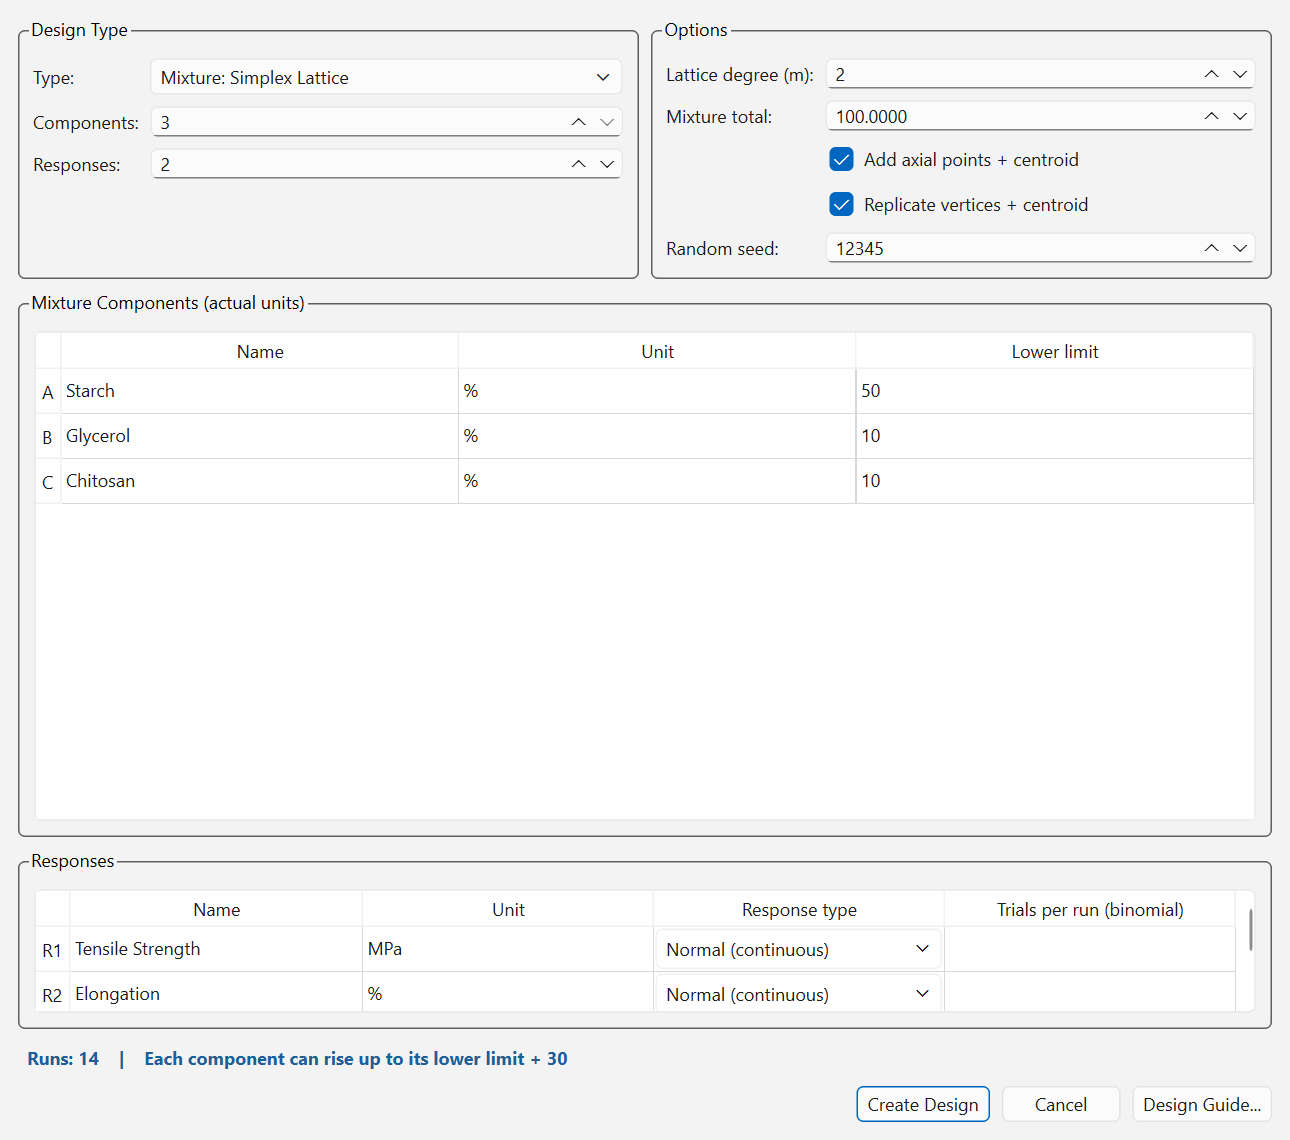
\includegraphics[width=0.75\linewidth]{new_design_mixture.png}
\caption{New Design dialog for a simplex lattice \{3,2\}: Starch (lower limit 50 \%), Glycerol (10 \%) and Chitosan
(10 \%), total 100. The information line shows 14 runs and that each component can rise up to its lower limit + 30.}
\label{fig:ch03-newmixture}
\end{figure}

\paragraph{Example: edible film.} The case study ``Edible Film Formulation (Mixture)'' (Figure~\ref{fig:ch03-newmixture})
has lower limits 50, 10 and 10 \% and total 100, so the span is $100 - 70 = 30$. The pseudo-component blend
(1/2, 1/2, 0) corresponds to Starch $50 + 0.5 \times 30 = 65$ \%, Glycerol $10 + 0.5\times 30 = 25$ \% and Chitosan
10 \%; the vertices are Starch 80 / Glycerol 40 / Chitosan 40 \%. On the Data page the check box \ui{Show
pseudo-components} switches between the two scales.

\section{Optimal (custom) designs}
\label{sec:ch03-optimal}

Optimal designs choose the runs from a set of candidate points so that a criterion is as good as possible for the
\emph{planned model} \citep{goos2011}. They are the right choice when the region is not a cube or simplex (linear
constraints, upper limits on components), when categorical and numeric factors are mixed, when the run budget does
not match a classical design, or when a mixture is combined with process factors. REGEN offers three types:
\ui{Optimal (Custom) - Process}, \ui{Mixture: Optimal (Custom)} and \ui{Combined Mixture + Process (Optimal)}.

\paragraph{Structure of the design.} An optimal design in REGEN has three parts:
\begin{itemize}
\item \emph{model points}: $n_m = p + {}$\ui{Additional model points}, chosen by the D or I criterion (type
``Model''); $p$ is the number of model coefficients, including the effect-coded columns of categorical factors;
\item \emph{lack-of-fit points}: \ui{Lack of fit points} extra distinct points, each as far as possible from the
points already chosen (type ``Lack of Fit''), so that the model can be checked;
\item \emph{replicates}: the \ui{Replicate points} distinct model points with the highest leverage are repeated
(type ``Replicate''), giving pure error.
\end{itemize}
The total is $n = p + \text{extra} + n_{\text{LOF}} + n_{\text{rep}}$. With the defaults, a two-factor quadratic
model gives $6 + 5 + 5 = 16$ runs.

\subsection{Linear constraints}
\label{sec:ch03-constraints}
For the optimal types the dialog shows the box \ui{Linear Constraints (one per line, actual units, letters =
factors/components)}. Each line is one inequality in actual units, for example
\begin{verbatim}
A + B <= 150
2A - B >= 50
\end{verbatim}
The operators \texttt{<=}, \texttt{>=}, \texttt{=<}, \texttt{=>} are accepted; \texttt{<} and \texttt{>} are
treated as $\le$ and $\ge$. Terms are written as \texttt{2A}, \texttt{2*A}, \texttt{0.5B} or \texttt{A};
constants may appear on either side; a decimal comma is accepted; letters are case-insensitive. Error messages are
``A constraint must use <= or >=.'', ``The constraint contains no factors.'', ``Factor 'X' does not exist (use
letters A--C).'' and ``Cannot read '\dots'.'', each prefixed by the line number. Constraints cannot contain
categorical factors, and in a combined design only the mixture components may appear.

Internally a constraint $a^\top x \le b$ is converted to coded units with $x = o + s \odot z$ (offset $o$ and scale
$s$ of Equation~\ref{eq:ch03-coding} or~\ref{eq:ch03-pseudo}):
\begin{equation}
G z \le h, \qquad G = a \odot s, \qquad h = b - a^\top o,
\label{eq:ch03-constraint}
\end{equation}
with $\ge$ rows multiplied by $-1$. The same constraints are respected later in region sampling (Design Evaluation,
Data Readiness) and in optimization.

\subsection{Candidate points}
The design region is the set of $z$ satisfying the bounds ($-1 \le z \le 1$ for process factors; $L \le z \le U$
with $\sum z = 1$ for mixtures) and $Gz \le h$. The candidate set contains:
\begin{enumerate}
\item the \emph{vertices} of this polytope: every combination of $d$ inequalities ($d-1$ plus the mixture equation
for mixtures) is solved as an equation system; feasible, distinct solutions are vertices;
\item \emph{edge midpoints}: the midpoint of two vertices that share at least $\dim - 1$ active constraints;
\item \emph{face centers}: the mean of the vertices on a constraint face with at least three vertices;
\item the \emph{overall centroid}, the mean of all vertices;
\item \emph{axial points} halfway between each vertex and the centroid;
\item for process factors only, the three-level grid $\{-1, 0, 1\}^d$ inside the bounds.
\end{enumerate}
Infeasible points and duplicates are removed. Process candidates are crossed with all categorical level
combinations; in a combined design each mixture candidate is crossed with the $3^{n_{\text{proc}}}$ grid of the
process factors. If the candidate matrix cannot support the model (rank $< p$), the message ``There are not enough
candidate points to estimate this model. Relax the constraints or choose a simpler model.'' appears; if the bounds
and constraints contradict each other: ``The design region is empty: the bounds and constraints contradict each
other.''

\subsection{Criteria}
Let $X$ be the model matrix of the chosen points and $M = X^\top X + 10^{-8} I$ (the small ridge keeps $M$
invertible during the search).
\begin{description}[leftmargin=0pt]
\item[D-optimal (best coefficients)] maximizes $\log\det M$. This minimizes the volume of the joint confidence
region of the coefficients; it favors points at the boundary of the region.
\item[I-optimal (best prediction)] minimizes the average prediction variance over the region,
\begin{equation}
I = \operatorname{tr}\bigl(M^{-1} W\bigr), \qquad W = \frac{1}{N_R}\, F^\top F,
\label{eq:ch03-icrit}
\end{equation}
where $F$ is the model matrix of $N_R = 3000$ points drawn uniformly from the region (uniform in the box for
process factors; for mixtures $z = L + (1 - \sum L)\,\text{Dirichlet}(1, \dots, 1)$, rejecting points above an
upper bound; points violating constraints are rejected; categorical levels at random). If fewer than 50 region
points survive, the candidate set is used instead. I-optimal designs put more points in the interior and are
recommended when the purpose is prediction and optimization \citep{goos2011}.
\end{description}

\subsection{Exchange algorithm}
The model points are found with a Fedorov-type exchange algorithm \citep{cook1980}. The search starts from $n_m$
random candidates; at each iteration every swap of a candidate $x_j$ (not yet in the design) for a design point
$x_i$ is evaluated with rank-two update formulas and the single best swap is made. With
$d_{jj} = x_j^\top M^{-1} x_j$, $d_{ii} = x_i^\top M^{-1} x_i$ and $d_{ij} = x_j^\top M^{-1} x_i$, the ratio of the
determinants after and before the swap is
\begin{equation}
\Delta_D = \frac{\det M'}{\det M} = (1 + d_{jj})(1 - d_{ii}) + d_{ij}^2 ,
\label{eq:ch03-fedorov}
\end{equation}
and the search stops when $\max \Delta_D \le 1 + 10^{-9}$. For the I criterion, with $G = M^{-1} W M^{-1}$ and
$g_{jj}, g_{ii}, g_{ij}$ defined like $d$, the reduction of $I$ follows from the Woodbury identity,
\begin{equation}
\Delta_I = \frac{(d_{ii}-1)\,g_{jj} - 2\,d_{ij}\,g_{ij} + (1+d_{jj})\,g_{ii}}{(1+d_{jj})(d_{ii}-1) - d_{ij}^2},
\label{eq:ch03-iswap}
\end{equation}
and the search stops when $\max \Delta_I \le 10^{-10}$. At most 300 iterations are made per start, from six random
starts; the best result is kept. Model points are distinct (a candidate already in the design cannot be swapped in).
Coordinate exchange \citep{meyer1995}, which works without a candidate list, is not used.

\paragraph{Lack-of-fit and replicate points.} Lack-of-fit points are added one at a time: the remaining candidate
with the largest minimum Euclidean distance to all chosen points (categorical factors one-hot encoded and divided
by $\sqrt{2}$, so that a level change counts as distance 1). Replicates are the distinct chosen points with the
highest leverage $h = x^\top (X^\top X)^{+} x$.

\paragraph{Reproducibility.} The random starts and the region sample use the \ui{Random seed:}. The same seed and
settings give the same design.

\paragraph{Example: constrained D-optimal design.} Two factors, Temperature 60--80 \textdegree C (A) and Time
30--90 min (B), with the constraints shown above, a quadratic model, D-optimal, seed 12345. The region is a pentagon
with vertices (60, 30), (60, 70), (80, 30), (80, 70) and (66.67, 83.33); the candidate set has 19 points (5
vertices, 5 edge midpoints, the centroid, 5 axial points and 3 grid points). The info line reads ``Model Quadratic:
6 coefficients $\rightarrow$ 16 runs in total (6 model + 5 lack of fit + 5 replicates)''. The six model points are
the five vertices and the centroid (69.33, 56.67); the lack-of-fit points are (70, 30), (73.33, 76.67), (60, 50),
(80, 50) and (74.67, 43.33); the five replicates repeat the five vertices. The design description is
``Optimal (Custom) - Process (D-optimal, model Quadratic) - 2 factors, 2 constraints, 16 runs''.

\begin{figure}[htbp]
\centering
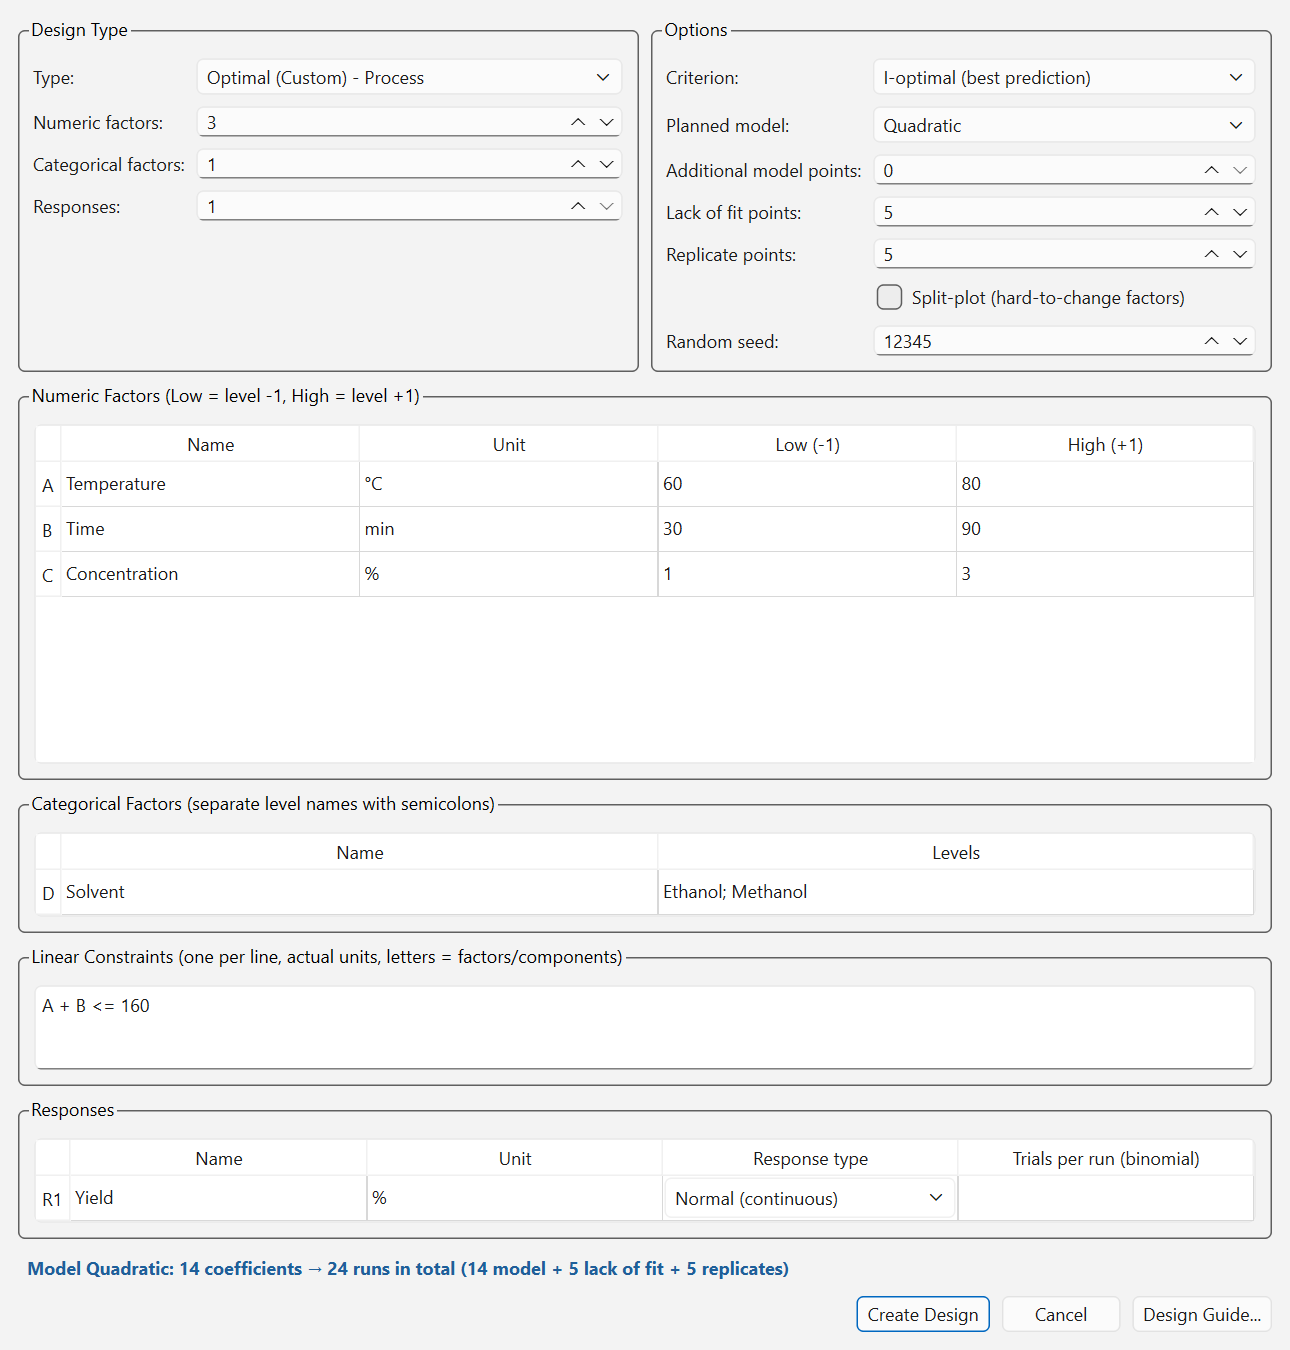
\includegraphics[width=0.75\linewidth]{new_design_optimal.png}
\caption{New Design dialog for an I-optimal process design: three numeric factors, one categorical factor Solvent
(Ethanol; Methanol), constraint \texttt{A + B <= 160}, quadratic model. Info line: ``Model Quadratic: 14
coefficients $\rightarrow$ 24 runs in total (14 model + 5 lack of fit + 5 replicates)''.}
\label{fig:ch03-newoptimal}
\end{figure}

\paragraph{I-optimal or D-optimal?} For three factors, a quadratic model and seed 12345, the ten model points of the
I-optimal design have an average prediction variance of $0.732\sigma^2$ against $0.857\sigma^2$ for the D-optimal
model points, while the D-optimal model points have the slightly larger D-efficiency (40.95 \% against 40.43 \%).
The criterion is applied to the model points only; the lack-of-fit and replicate points added afterwards change the
final values, so the complete 20-run designs can rank differently (Chapter~\ref{chap:4} compares them).

\subsection{Combined mixture and process designs}
A combined design studies $q$ mixture components and 1--4 process factors (for example a dough recipe and the
baking temperature). The model is the product of a Scheff\'e mixture model (without the cubic $\delta$ terms) and a
process model: every mixture term is multiplied by every process term. The order is written as \ui{Mixture
$\times$ Process}, for example \ui{Quadratic $\times$ Linear} (the default): the six quadratic Scheff\'e terms of
three components times (1, T) give 12 coefficients. The available orders are Linear $\times$ Mean, Linear $\times$
Linear, Linear $\times$ 2FI, Quadratic $\times$ Linear, Quadratic $\times$ 2FI, Quadratic $\times$ Quadratic,
Special Cubic $\times$ Linear and Special Cubic $\times$ 2FI. Process factors are coded $-1 \dots +1$; in the
I-optimal region sample they are uniform on $[-1, 1]$. The case study ``Cake Dough + Baking Temperature (Combined)''
(Flour 50--80, Sugar 10--30, Fat 10--30 \%, total 100; Temperature 160--200 \textdegree C) has 22 runs: 12 model, 5
lack-of-fit and 5 replicate points.

\section{Space-filling designs for neural networks}
\label{sec:ch03-spacefilling}

\subsection{Maximin Latin hypercube}
A Latin hypercube with $n$ points \citep{mckay1979} gives every factor $n$ equally spaced levels between $-1$ and
$+1$ (both bounds included), each used exactly once. Random Latin hypercubes can leave points clustered, so REGEN
rearranges the levels to spread the points as evenly as possible, using the Morris--Mitchell criterion
\citep{morris1995}
\begin{equation}
\phi_p = \sum_{i<j} d_{ij}^{-p}, \qquad p = 15,
\label{eq:ch03-phip}
\end{equation}
where $d_{ij}$ is the Euclidean distance between points $i$ and $j$ in coded units. For large $p$, minimizing
$\phi_p$ maximizes the smallest distance between points (maximin) and, among designs with the same smallest
distance, reduces the number of pairs at that distance.

\paragraph{Algorithm.} The search starts with an independent random permutation for each column and improves it by
simulated annealing: pick a random column and two runs, swap their levels, update $\phi_p$ incrementally, accept the
swap if $\phi_p$ decreases or otherwise with probability $e^{-\Delta\phi/T}$. The start temperature is
$T_0 = 0.02\,\phi_0$, it is multiplied by 0.9995 each iteration, and the number of iterations is
$\min(20000, 200n)$. For $n \le 60$ two independent starts are made and the better one kept. Above 2000 points a
plain random Latin hypercube is returned without optimization. The Latin hypercube property means that each factor
is sampled uniformly over its whole range, which reduces the variance of averages compared with random sampling
\citep{stein1987}.

\paragraph{Center points.} The default 4 center points are replicated runs at the center; they are not needed for
the space filling but give an estimate of the pure error, which the ANN diagnosis uses to recognize overfitting.

\paragraph{Example.} For three factors and seed 12345, the smallest distance between two of 20 maximin points is
0.547 coded units (a random Latin hypercube of the same size: 0.182); with 40 points it is 0.404 (random: 0.089).

\subsection{Hybrid RSM and space-filling design}
The hybrid type combines a classical RSM base design without center points (\ui{CCD face-centered (3 level)},
\ui{CCD rotatable (5 level)}, \ui{Box-Behnken (3 level)} or \ui{Factorial (2 level)}) with $e$ space-filling points
and center points. The extra points are chosen by greedy maximin: a candidate pool of a Latin hypercube with
$\max(4e, 20)$ points (2000 annealing iterations) plus 4000 uniform random points is formed, and repeatedly the
candidate whose distance to the nearest existing point (base design and the center) is largest is added. The RSM
model keeps its classical structure, while the ANN receives many more levels per factor. Example: CCD
face-centered for three factors (14 points) + 12 space-filling points + 4 center points = 30 runs. The Box-Behnken
base needs at least three factors (``Box-Behnken requires at least 3 factors.'').

\section{Split-plot designs}
\label{sec:ch03-splitplot}
When a factor is hard or expensive to change (an oven temperature, a reactor pressure), complete randomization would
require resetting it for every run. In a split-plot design the runs with the same setting of the hard-to-change
(HTC) factors are grouped into \emph{whole plots}; within a whole plot only the easy-to-change factors vary
\citep{goos2011}. Tick \ui{Split-plot (hard-to-change factors)} (available for full factorial, general factorial,
CCD, BBD and optimal process designs), type the HTC letters in \ui{Hard-to-change factors:} and set \ui{Runs per
whole plot:}.

\paragraph{Construction.} Runs with identical HTC settings form a group. A group larger than the whole-plot size is
split in standard order; the automatic size is $\lceil m/2 \rceil$ for a group of $m$ runs, so every HTC setting
appears in at least two whole plots and the whole-plot error can be estimated. The runs are randomized within each
whole plot, and the whole plots are run in random order. Blocks are not used. The Data page shows an extra column
\ui{WP}, and the design description ends with, for example, ``split-plot (HTC: A; 4 whole plots)''.

\paragraph{Analysis.} Because the whole plots are a second source of random variation, the analysis uses a mixed
model fitted by REML (Chapter~\ref{chap:5}). Whole-plot factors are tested against the whole-plot error, which has few degrees
of freedom, so their tests are less powerful than those of the subplot factors.

\paragraph{Example.} The case study ``Oven Product Hardness (Split-Plot)'' is a 2\textsuperscript{3} full
factorial with two replicates (16 runs), HTC factor A (Oven Temperature) and 4 runs per whole plot, which gives 4
whole plots (Figure~\ref{fig:ch04-datasplit} in Chapter~\ref{chap:4}). Augmentation is not available for split-plot
designs: the \ui{Augment Design\dots} button is disabled and its tooltip reads ``Augmenting split-plot designs is not
supported: the new runs would need their own whole plots. Create a new split-plot design instead.''

\section{Historical data}
\label{sec:ch03-historical}
The type \ui{Historical Data (Process)} creates \ui{Data rows:} empty rows (default 20) with point type
``Historical''. On the Data page the factor cells are then editable as well as the response cells; categorical
factors take the level name or the level number. \ui{Add Rows} and \ui{Delete Selected Rows} appear for this type.
Historical data are rarely orthogonal: check them on the Design Evaluation page (VIF, correlations, efficiencies)
and the Data Readiness page before trusting a model. Existing tables are more conveniently loaded with
\menupath{File $\rightarrow$ Import Data\dots}, which also creates historical mixture projects.

\section{Categorical factors}
\label{sec:ch03-categoric}
Categorical factors (solvent type, supplier, catalyst) are allowed in full factorials, general factorials, CCD,
BBD, optimal process designs, historical data, Latin hypercube and hybrid designs (0--4 factors). Enter the level
names separated by semicolons (commas are also accepted). Except for optimal designs, the numeric design is
repeated for every combination of categorical levels (full crossing), so the run count is multiplied by
$\prod_c L_c$; the information line shows for example ``Runs: 33 (11 $\times$ 3 categorical level combinations)''
for a two-factor CCD with three center points and three solvents (case study ``Extraction with Solvent Type
(Categoric)''). In an optimal design the categorical levels are part of the candidate set, and the exchange
algorithm decides how many runs each level receives; this is much cheaper when there are several categorical
factors.

\section{Randomization and the random seed}
\label{sec:ch03-random}
Runs must be performed in random order so that drifts in equipment, materials or operators do not bias the effects
\citep{montgomery2017}. REGEN assigns a random run order: a random permutation of all runs, or, in blocked designs,
a random permutation within each block with the blocks in sequence. The \ui{Std} column keeps the standard
(construction) order; the \ui{Run} column gives the order in which to perform the runs.

\paragraph{Random seed.} The option \ui{Random seed:} (1--999\,999\,999) initializes the random numbers used for the
run order, the whole-plot order of split-plot designs and the random parts of optimal, Latin hypercube and hybrid
designs. A new random value is drawn each time the dialog opens. The same seed with the same settings creates
exactly the same design again; note the seed (it is saved in the project and shown on the Summary page), or type a
fixed value, when the design must be reproducible, for example in a report or a course. All screenshots in this
manual use seed 12345.

\section{The Design Guide}
\label{sec:ch03-guide}

\paragraph{Purpose.} The \ui{Design Guide} answers two questions before any run is made: which design suits the
goal, and how many runs are needed for an RSM model or an ANN.

\paragraph{How to open.} \menupath{File $\rightarrow$ Design Guide\dots}, \menupath{Help $\rightarrow$ Design
Guide (RSM / ANN Run Counts)\dots}, the toolbar button \ui{Design Guide}, \ui{Design guide} on the Start Page, or
\ui{Design Guide\dots} inside the New Design dialog. The guide has three tabs. \ui{Create This Design\dots} (or a
double-click on a row or cell) closes the guide and fills the New Design dialog with the chosen type, number of
factors and options; it is available on the first two tabs.

\subsection{Recommendations by goal}
\label{sec:ch03-guide-goal}
\paragraph{Options.} \ui{Goal:} (default ``RSM optimization: find the optimum (curvature present)''),
\ui{Numeric factors:} (1--21), \ui{Max run budget:} (0 = ``no limit'') and, for the ANN goals only,
\ui{Nonlinearity:} (``Low (close to quadratic)'', ``Medium'', ``High (many peaks / sharp)''). A short explanation
of the goal appears below the options.

\paragraph{Output.} The table lists the proposed designs with \ui{Runs}, \ui{Levels per factor}, \ui{Model},
\ui{Power (2$\sigma$ signal)} and \ui{Notes}; designs above the budget are grey and marked ``over budget''. The
first suitable row is selected and explained below the table: advantages, disadvantages, the lowest power among the
model coefficients with the residual degrees of freedom, the number of coefficients of the model and an ANN verdict
for the run count (Section~\ref{sec:ch03-guide-calc}).

\paragraph{Rules.} The run counts are obtained by actually building each design. The rules per goal are:
\begin{itemize}
\item \emph{Screening}: Plackett--Burman with the smallest $N \in \{12, 20, 24\}$ larger than $k$; the fractional
factorial with the fewest runs and resolution $\ge$ IV plus 4 center points (a full factorial when no such fraction
exists); a DSD for $3 \le k \le 20$.
\item \emph{Ruggedness test} (``confirm that the factors have NO effect''): Plackett--Burman and the smallest
fraction with resolution $\ge$ III.
\item \emph{Characterization}: the smallest fraction of resolution $\ge$ V plus 4 center points; the full factorial
2\textsuperscript{k} + 4 center points when $k \le 7$ and no cheaper resolution V fraction exists; an optimal 2FI
design with $p + 5 + 5$ runs.
\item \emph{RSM optimization} and \emph{RSM and ANN}: rotatable and face-centered CCD with default center points
($2 \le k \le 6$), Box--Behnken ($3 \le k \le 7$) and an optimal quadratic design with $p + 5 + 5$ runs. For
$k \ge 6$ an extra row ``Suggestion: screen first'' proposes a DSD.
\item \emph{ANN modeling}: a Latin hypercube with the ANN target (below) plus 4 center points, and the minimum
Latin hypercube plus 3 center points.
\item \emph{ANN} and \emph{RSM and ANN}: hybrid designs on CCD face-centered, Box--Behnken ($k\ge 3$) and CCD
rotatable bases with $e = \max(\text{target} - n_{\text{base}} - 4, 6)$ space-filling points and 4 center points.
\item If the budget is below the ANN minimum, a row ``Budget of B runs is below the ANN minimum'' appears; if no
Latin hypercube fits the budget, a Latin hypercube with $B - 3$ runs + 3 center points is proposed.
\end{itemize}

\paragraph{Power.} The power column is the smallest power over all non-intercept coefficients of the model, computed
as on the Design Evaluation page (Chapter~\ref{chap:4}) with signal $\Delta = 2$, noise $\sigma = 1$ and $\alpha = 0.05$: the
probability of detecting a coefficient whose low-to-high effect equals two standard deviations. Optimal designs show
no power because they are not built in the guide. For three factors the values are: CCD rotatable 20 runs 72 \%,
CCD face-centered 20 runs 32 \%, Box--Behnken 17 runs 41 \% (the weakest terms are the interactions or the squared
terms).

\begin{figure}[htbp]
\centering
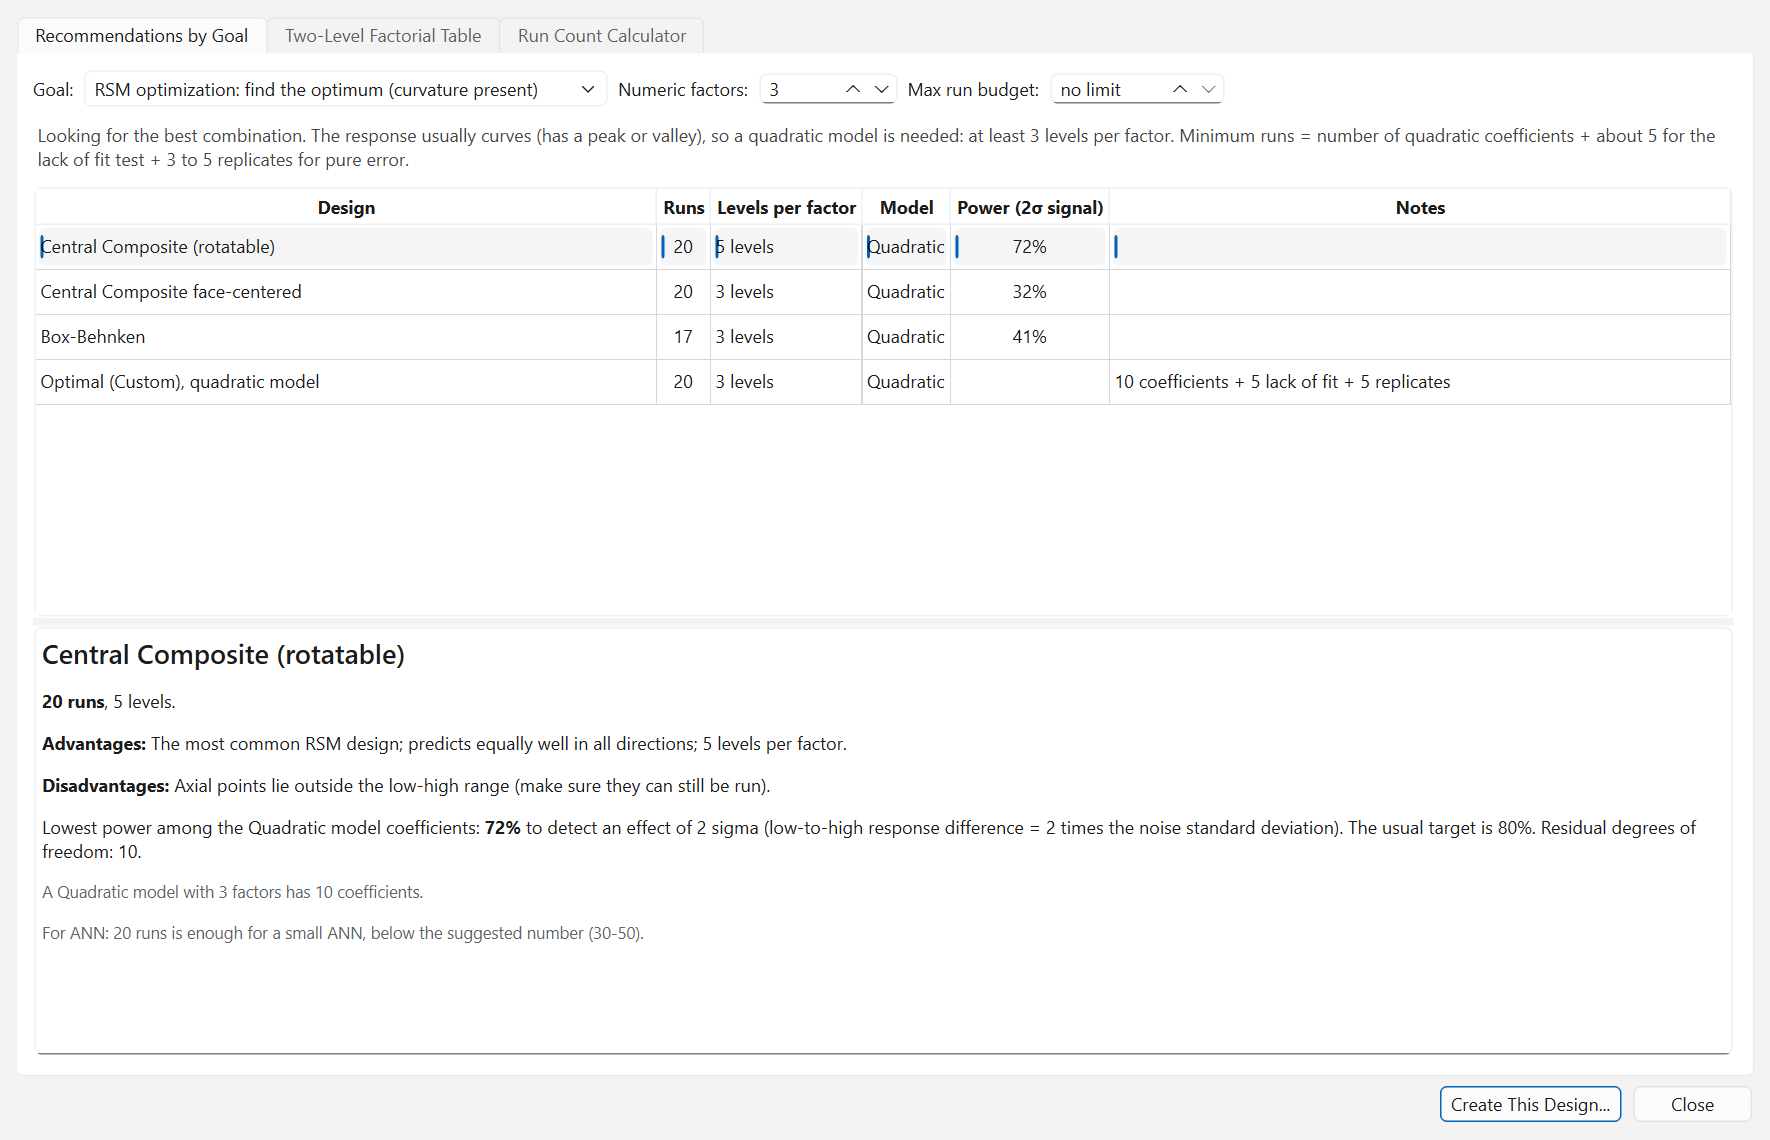
\includegraphics[width=\linewidth]{design_guide_recommend.png}
\caption{Design Guide, tab Recommendations by Goal: goal RSM optimization, 3 numeric factors. The rotatable CCD (20
runs, 5 levels, lowest power 72 \%) is selected and explained below the table.}
\label{fig:ch03-guiderec}
\end{figure}

\subsection{Two-level factorial table}
\label{sec:ch03-guide-table}
This tab shows all two-level designs for 2--21 factors (columns) and 4--512 runs (rows). Each cell gives
2\textsuperscript{k} ``full'' or 2\textsuperscript{k-p} with its resolution; the colors are white for full
factorials, green for resolution V and higher (clean main effects and two-factor interactions: characterization),
yellow for resolution IV (clean main effects: screening), red for resolution III (main effects aliased with
two-factor interactions: ruggedness testing) and grey where no design exists. \ui{Replicates:} (1--10) and
\ui{Center points:} (0--50) change the run count $N = 2^{k-p} \times \text{replicates} + \text{center points}$;
\ui{Show Generators} writes the generators into the cells of fractions with $p \le 3$.

Clicking a cell shows the design: the number of runs, the meaning of its resolution, the generators, the defining
relation (first 12 words), the word length pattern with the reminder that fewer short words mean lower aberration,
and a table of the aliases of main effects and two-factor interactions with effects of up to three letters. A note
recalls that two-level designs cannot model curvature and are not suitable for ANN or quadratic models.

\begin{figure}[htbp]
\centering
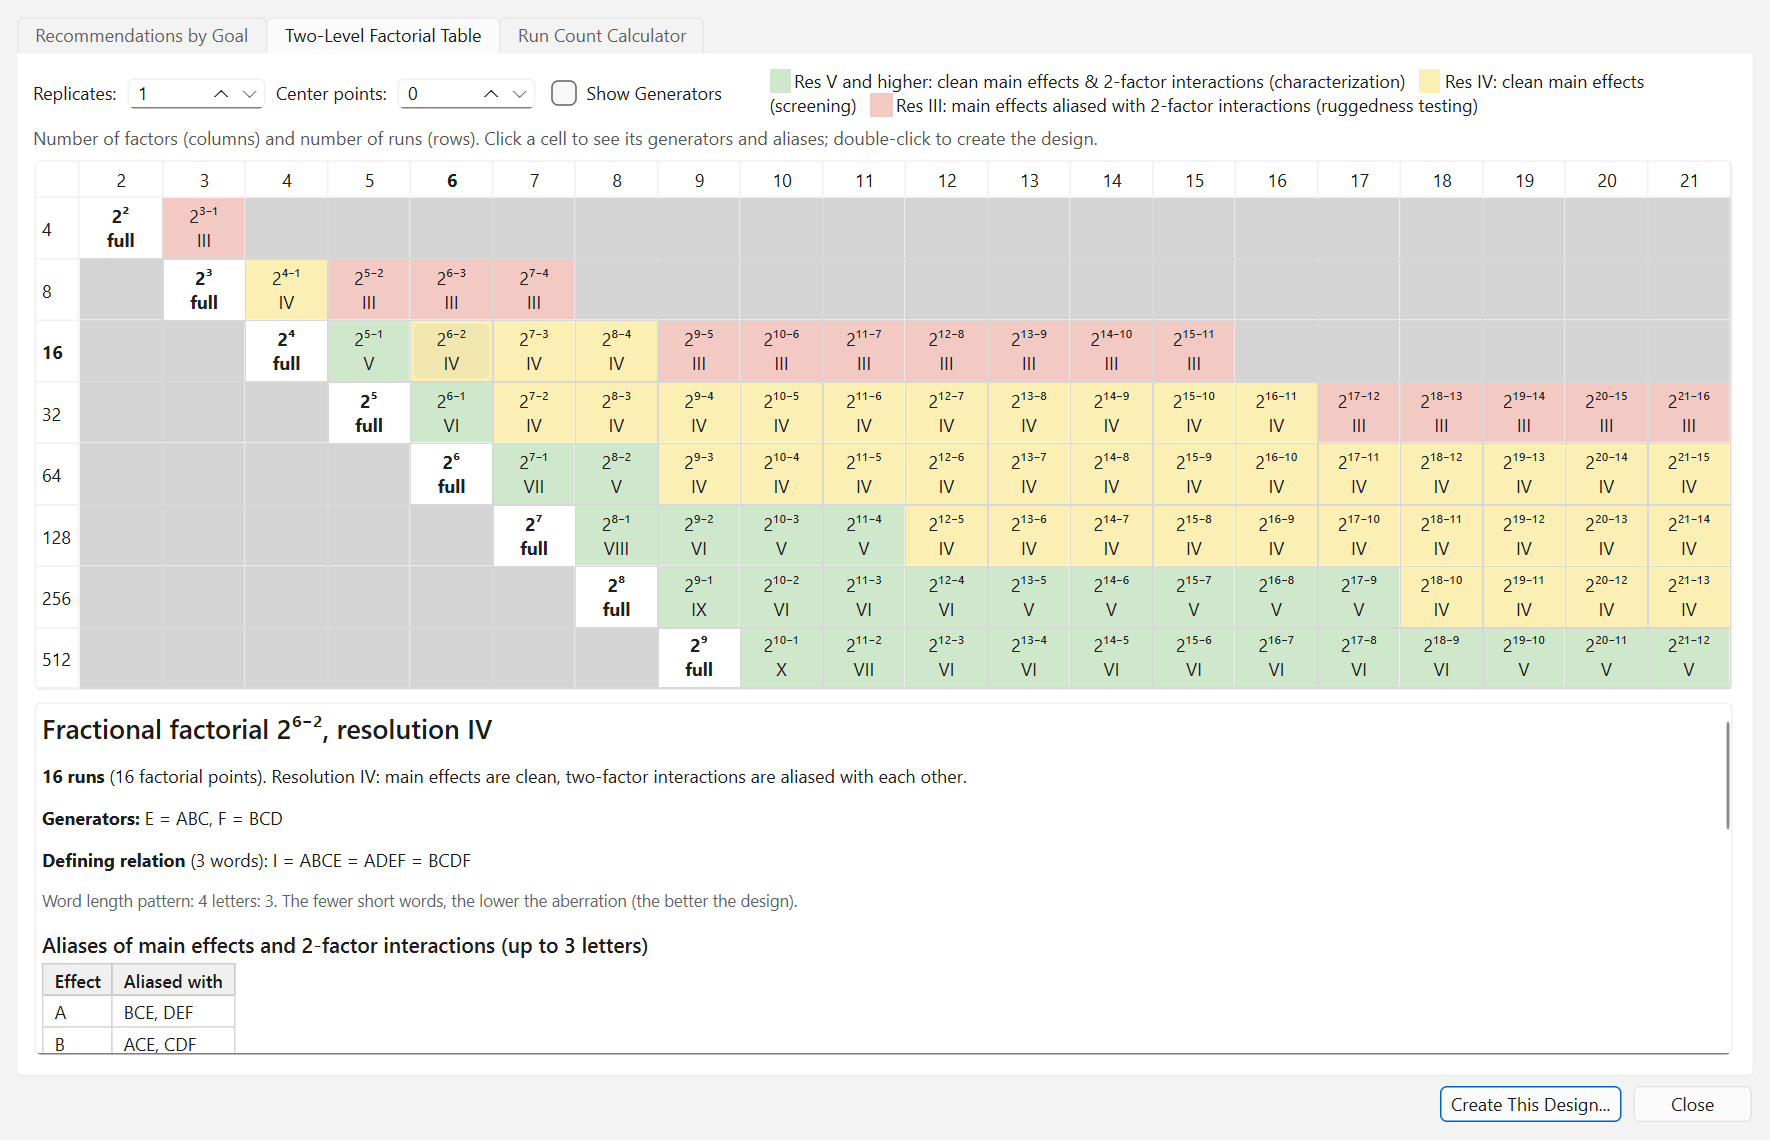
\includegraphics[width=\linewidth]{design_guide_table.png}
\caption{Design Guide, tab Two-Level Factorial Table. The selected cell (16 runs, 6 factors) is the
2\textsuperscript{6-2} of resolution IV with generators E = ABC, F = BCD, defining relation I = ABCE = ADEF = BCDF
and word length pattern ``4 letters: 3''.}
\label{fig:ch03-guidetable}
\end{figure}

\subsection{Run count calculator}
\label{sec:ch03-guide-calc}
\paragraph{RSM.} Inputs: \ui{Numeric factors:} (1--21), \ui{Model:} (Linear, 2FI, Quadratic, Cubic),
\ui{Lack of fit points:} (default 5) and \ui{Replicate points:} (default 5). With $p$ from
Equation~\ref{eq:ch03-ncoef}:
\begin{equation}
n_{\text{abs}} = p + 1, \qquad n_{\text{rec}} = p + n_{\text{LOF}} + n_{\text{rep}} .
\label{eq:ch03-rsmruns}
\end{equation}
$n_{\text{abs}}$ is the absolute minimum (one degree of freedom for the error); $n_{\text{rec}}$ is the
recommendation, which allows a lack-of-fit test and an estimate of pure error. The table ``Standard designs for k
factors'' lists the full factorial with 4 center points and the smallest suitable fraction (linear and 2FI models,
$k \le 9$), the rotatable and face-centered CCD ($2 \le k \le 6$) and the Box--Behnken design ($3 \le k \le 7$)
with their residual degrees of freedom and lowest power (``not enough df'' when there is no residual df). Below
80 \% power, add replicates or center points, or accept that small effects may go undetected.

\paragraph{ANN.} Inputs: \ui{Neurons per hidden layer:} (empty = automatic, $2k$ neurons in one layer; several
layers as a comma or semicolon separated list), \ui{Number of outputs:}, \ui{Algorithm:} (``Bayesian Regularization
(trainbr)'' or ``Levenberg-Marquardt / Adam''), \ui{Validation:} (``k-fold cross-validation (data < 400)'' or
``Hold-out 70/15/15 (large data)'') and \ui{Data you have:}. The number of weights and biases of a network with
$k$ inputs, hidden layers $h_1, \dots, h_L$ and $n_{\text{out}}$ outputs is
\begin{equation}
W = \sum_{l=1}^{L} h_l\,(h_{l-1} + 1) + n_{\text{out}}\,(h_L + 1), \qquad h_0 = k .
\label{eq:ch03-weights}
\end{equation}
The training set should contain at least $rW$ rows, with ratio $r = 1$ for trainbr (Bayesian regularization reduces
the effective number of parameters) and $r = 2$ for Levenberg--Marquardt or Adam. Because only a fraction $f$ of the
runs is used for training ($f = 0.85$ with k-fold cross-validation, $0.70$ with hold-out), the runs needed are
\begin{equation}
n_{\text{need}} = \left\lceil \frac{r\,W}{f} \right\rceil .
\label{eq:ch03-annruns}
\end{equation}
Example: three factors and 6 hidden neurons give $W = 6 \cdot 4 + 1 \cdot 7 = 31$ and, with trainbr and k-fold,
$n_{\text{need}} = \lceil 31/0.85 \rceil = 37$; with Levenberg--Marquardt and hold-out, $\lceil 62/0.70 \rceil = 89$.

\paragraph{Rules of thumb.} Table~\ref{tab:ch03-ann} gives the practical guideline used throughout REGEN for the
number of ANN runs (trainbr with cross-validation). The \emph{ANN target} used by the guide and as the default
number of Latin hypercube points is the lower recommended value for low nonlinearity, the integer mean of the
recommended range for medium nonlinearity and the larger of the upper value and the ``highly nonlinear'' value for
high nonlinearity. These numbers are a guideline, not a law: the spread of the points matters more than their
number (use at least 5 levels per factor), and the learning curve on the ANN page shows objectively whether more data
would still help.

\begin{table}[htbp]
\centering
\caption{Rule-of-thumb run counts for ANN models and the ANN target by nonlinearity.}
\label{tab:ch03-ann}
\small
\begin{tabular}{@{}ccccccc@{}}
\toprule
k & Minimum & Recommended & Highly nonlinear & Target low & Target medium & Target high \\
\midrule
1 & 10 & 15--20 & 30 & 15 & 17 & 30 \\
2 & 15 & 25--30 & 40 & 25 & 27 & 40 \\
3 & 20 & 30--50 & 60 & 30 & 40 & 60 \\
4 & 30 & 50--80 & 100 & 50 & 65 & 100 \\
5 & 40 & 70--120 & 150 & 70 & 95 & 150 \\
6 & 50 & 100--150 & 200 & 100 & 125 & 200 \\
$>6$ & $10k-10$ & $17k$--$25k$ & $35k$ & $17k$ & mean & $35k$ \\
\bottomrule
\end{tabular}
\end{table}

\paragraph{ANN verdict.} For $n$ runs and $k$ factors the verdict text (also shown in the New Design information
line for Latin hypercube and hybrid designs) is: below the minimum, ``n runs is below the practical minimum (\dots)
for k factors''; below the lower recommended value, ``enough for a small ANN, below the suggested number''; below
the highly nonlinear value, ``matches the suggested number''; otherwise ``enough for strongly nonlinear patterns''.

\paragraph{Your data.} When \ui{Data you have:} is set, the calculator states whether the data are enough for the
RSM model ($n \ge n_{\text{rec}}$) and gives the ANN verdict, adding ``This architecture needs about
$n_{\text{need}}$ runs'' when the data are fewer.

\begin{figure}[htbp]
\centering
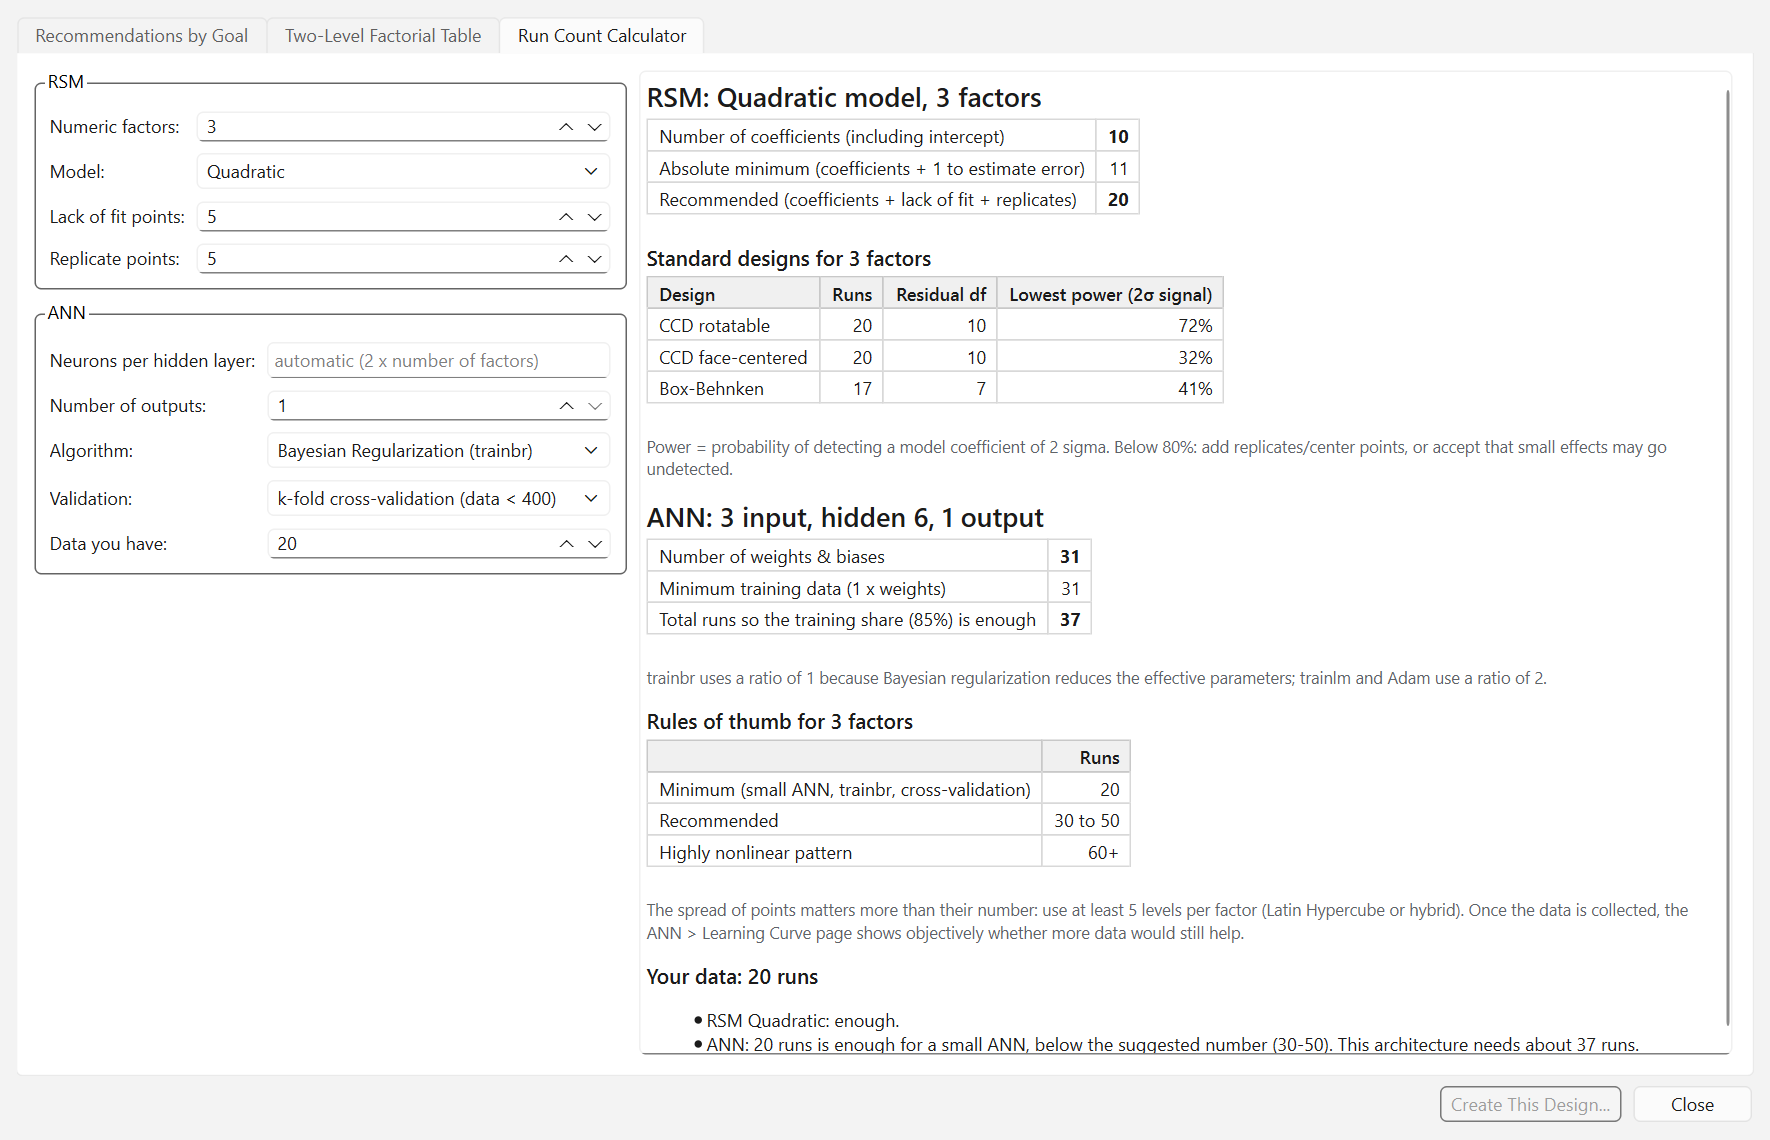
\includegraphics[width=\linewidth]{design_guide_calculator.png}
\caption{Design Guide, tab Run Count Calculator: 3 factors, quadratic model (10 coefficients, absolute minimum 11,
recommended 20 runs), standard designs with their power, and an ANN with automatic hidden size (6 neurons, 31
weights and biases) for ``Data you have'' = 20.}
\label{fig:ch03-guidecalc}
\end{figure}

\section{Augmenting a design}
\label{sec:ch03-augment}

\paragraph{Purpose.} Augmentation adds runs to an existing design without discarding the runs already made:
center points to check curvature or estimate pure error, replicates, axial points that turn a factorial into a
central composite design, or a fold-over that breaks aliases.

\paragraph{How to use.}
\begin{enumerate}
\item On the \ui{Data} page click \ui{Augment Design\dots} (not shown for historical data; disabled for
split-plot designs).
\item Choose the \ui{Type:} and set the count, alpha or fold-over factor.
\item Leave \ui{Make it a new block} checked when the new runs are made at a different time (recommended; the block
absorbs any shift between the two stages).
\item Click \ui{Add}. The message ``n new runs added. Enter their response values in the table.'' appears. The new
runs get run numbers after the current maximum, in random order among themselves, and empty responses.
\end{enumerate}

\begin{table}[htbp]
\centering
\caption{Options of the Augment Design dialog.}
\label{tab:ch03-augment}
\small
\begin{tabularx}{\linewidth}{@{}p{4.2cm}p{2.5cm}X@{}}
\toprule
Type & Available for & What is added \\
\midrule
\ui{Add center points} & all designs & \ui{Center points:} (1--50, default 3) center runs per categorical level
combination; for mixtures the overall centroid of the mixture region (type ``Centroid''). New block off by default. \\
\ui{Replicate the whole design} & all designs & \ui{Replicates:} copies of all runs with their point types. \\
\ui{Factorial $\rightarrow$ CCD (add axial + center points)} & full and fractional factorials, $\ge 2$ numeric
factors & $2k$ axial points at $\pm\alpha$ (\ui{Alpha:} Rotatable or Face-centered (alpha = 1)) plus
\ui{Additional center points:}, per categorical level combination. The design type becomes CCD. \\
\ui{Foldover (reverse signs)} & fractional factorials & A copy of all runs with all numeric signs reversed
(\ui{All factors (full foldover)}) or only one factor reversed (\ui{Only A: \dots}). Type ``Foldover''. \\
\bottomrule
\end{tabularx}
\end{table}

\paragraph{Theory as implemented.}
\begin{itemize}
\item \emph{Center points of a mixture.} The overall centroid of the (constrained) mixture region is the mean of the
vertices of the region; for a full simplex it is $(1/q, \dots, 1/q)$. Process factors of a combined design are set
to 0. For the case ``Cake Dough + Baking Temperature'' (vertices (50, 30, 20), (50, 20, 30), (80, 10, 10),
(60, 10, 30), (60, 30, 10)) the added centroid is Flour 60, Sugar 20, Fat 20 \%, whereas the mean of the existing
22 runs would be a different, unbalanced blend.
\item \emph{Factorial to CCD.} The rotatable axial distance is $\alpha = n_F^{1/4}$ with $n_F$ the number of
factorial runs of the core per categorical combination, replicates included \citep{myers2016}. A 2\textsuperscript{4}
(16 runs) gets $\alpha = 2$; a 2\textsuperscript{5-1} (16 runs) also gets $\alpha = 2$. For a fractional core the
description states it, for example ``axial points (alpha 2) on a 2\textasciicircum(5-1) fractional factorial
core''. The core must have resolution V or more for the quadratic model to be free of aliasing between
two-factor interactions.
\item \emph{Fold-over.} Reversing all signs of a resolution III fraction gives a combined design in which main
effects are no longer aliased with two-factor interactions \citep{montgomery2017}; reversing one factor frees that
factor and its two-factor interactions. For the 2\textsuperscript{7-4} (8 runs, Res III), the full fold-over gives
16 runs in which all seven main effects are orthogonal to each other and to the block (VIF 1, power 92.7 \% for
$\Delta = 2\sigma$ with the linear model).
\end{itemize}

\begin{figure}[htbp]
\centering
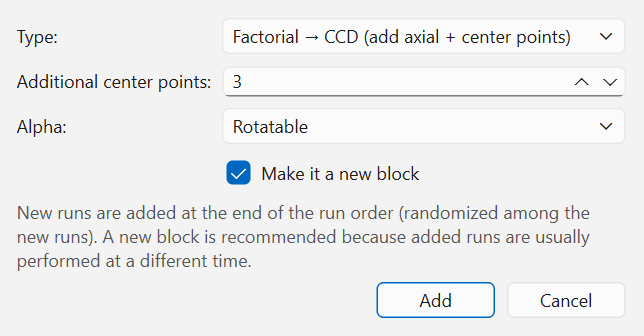
\includegraphics[width=0.6\linewidth]{augment_dialog.png}
\caption{Augment Design dialog for the 2\textsuperscript{4} factorial of the fermentation case: Factorial
$\rightarrow$ CCD with 3 additional center points, rotatable alpha, as a new block.}
\label{fig:ch03-augment}
\end{figure}

\paragraph{Example: from screening to optimization.} The case study ``Fermentation Screening (2\textasciicircum 4
Factorial)'' has 16 runs. Augmenting it with \ui{Factorial $\rightarrow$ CCD}, 3 center points and rotatable alpha
adds 8 axial points at $\pm 2$ and 3 center points in block 2. The design becomes ``Central Composite Design (CCD),
alpha = 2 + axial points (alpha 2) - 4 factors, 27 runs, 2 blocks'', which supports a quadratic model with a block
effect.

\paragraph{Other ways to add runs.} The Data Readiness page (Chapter~\ref{chap:4}) suggests runs computed from the current data
and model (D-optimal augmentation, gap filling, replicates, confirmation runs) and adds them with one click. For
historical data, rows are added with \ui{Add Rows}.

% Chapter 4: Data, Readiness and Design Evaluation
\chapter{Data, Readiness and Design Evaluation}\label{chap:4}
\label{ch:data}

After a design has been created (Chapter~\ref{chap:3}), the work moves to the pages of the groups \ui{Design} and
\ui{Project} in the navigation tree. The \ui{Data} page holds the design matrix and the measured responses;
\ui{Data Readiness} checks whether the data are good enough for modeling and optimization and suggests extra runs;
\ui{Design Evaluation} judges the design itself, before or after the experiment, without using any response values.
The project pages \ui{Summary}, \ui{Notes} and \ui{Column Graphs}, the \ui{Coefficient Table} and the tool
\ui{Data Normalization} complete the picture. The examples use the built-in case studies (\menupath{File
$\rightarrow$ Case Studies\dots}).

\section{The Data page}
\label{sec:ch04-data}

\paragraph{Purpose.} The \ui{Data} page (title ``Data \& Design'') shows every run of the design with its factor
settings and is the place where the measured responses are entered.

\begin{figure}[htbp]
\centering
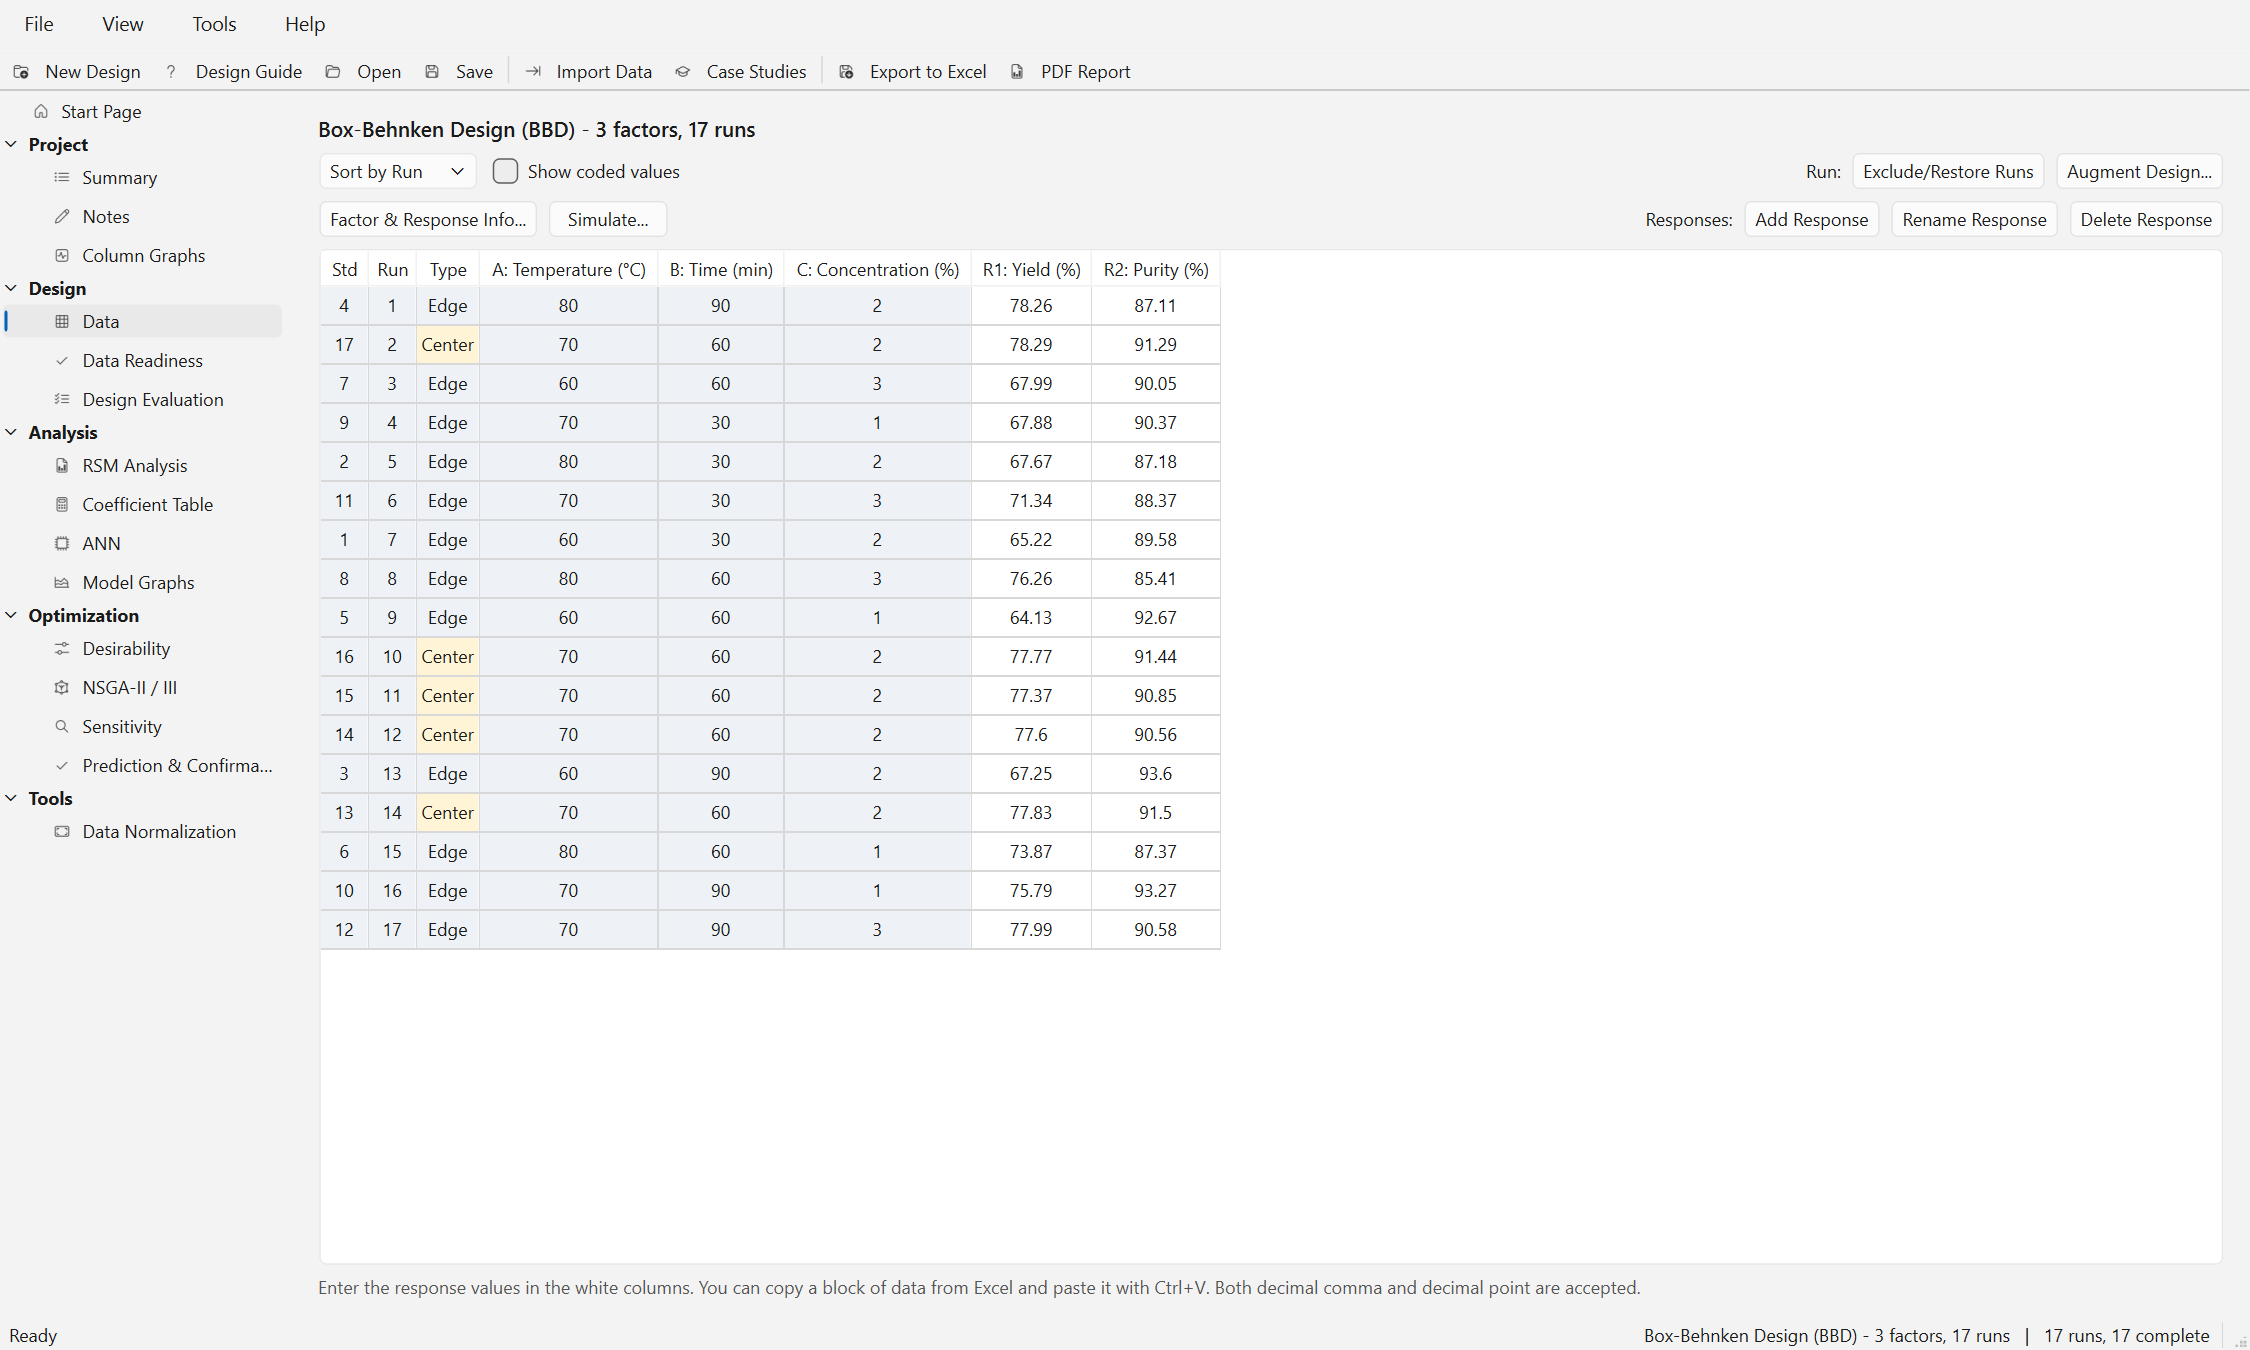
\includegraphics[width=\linewidth]{data_page.png}
\caption{Data page of the case study ``Extraction Optimization (Box-Behnken)'': 17 runs sorted by run order, point
types Edge and Center, grey read-only factor columns and white response columns Yield and Purity.}
\label{fig:ch04-datapage}
\end{figure}

\paragraph{Layout.} The bold line at the top is the design description, for example ``Box-Behnken Design (BBD) - 3
factors, 17 runs''. The first toolbar row contains the sort selector (\ui{Sort by Run} or \ui{Sort by Std}), the
check box \ui{Show coded values} (\ui{Show pseudo-components} for mixtures), \ui{Add Rows} and \ui{Delete Selected
Rows} (historical data only), \ui{Exclude/Restore Runs} and \ui{Augment Design\dots} (not for historical data).
The second row contains \ui{Factor \& Response Info\dots}, \ui{Simulate\dots} and the response buttons \ui{Add
Response}, \ui{Rename Response} and \ui{Delete Response}. The status bar at the bottom of the window repeats the
design description and shows ``N runs, F complete'' (F = runs with all responses filled) and, if any, ``m
excluded''.

\paragraph{Columns.} Table~\ref{tab:ch04-columns} describes the columns of the data sheet.

\begin{table}[htbp]
\centering
\caption{Columns of the data sheet.}
\label{tab:ch04-columns}
\small
\begin{tabularx}{\linewidth}{@{}p{3.2cm}X@{}}
\toprule
Column & Meaning \\
\midrule
\ui{Std} & Standard order: the position of the run in the design as constructed (1, 2, \dots). \\
\ui{Run} & Run order: the randomized order in which the experiments must be performed. \\
\ui{Block} & Block number (only when the design has more than one block). \\
\ui{WP} & Whole plot (split-plot designs only). \\
\ui{Type} & Point type (Table~\ref{tab:ch04-types}); ``(excluded)'' is appended for excluded runs. \\
A: Name (unit), \dots & Factor settings in actual units (or coded / pseudo-component values when the check box is
on, 6 significant digits). Categorical factors show the level name. Grey = read-only. \\
R1: Name (unit), \dots & Responses. White = editable. Empty = not yet measured. \\
\bottomrule
\end{tabularx}
\end{table}

\begin{table}[htbp]
\centering
\caption{Point types in the Type column.}
\label{tab:ch04-types}
\small
\begin{tabularx}{\linewidth}{@{}p{3.4cm}X@{}}
\toprule
Type & Origin \\
\midrule
Factorial & corner points of factorial designs and of the CCD \\
Center & center points (shaded yellow) \\
Axial & CCD axial points and mixture check blends (green) \\
Edge & Box--Behnken runs; mixture blends of two components \\
Screening & Plackett--Burman and definitive screening runs \\
Orthogonal & Taguchi array runs \\
Space-filling & Latin hypercube and hybrid extra points; gap-filling runs from Data Readiness \\
Vertex, Interior, Centroid & mixture blends (vertex blue, interior purple, centroid yellow) \\
Model, Lack of Fit, Replicate & the three parts of an optimal design \\
Historical & historical or imported data \\
Foldover & runs added by a fold-over \\
D-optimal, Mid-level, Replicate, Confirmation & runs added from the Data Readiness page \\
\bottomrule
\end{tabularx}
\end{table}

\paragraph{Run order and standard order.} Perform the experiments in the order of the \ui{Run} column
(\ui{Sort by Run}, the default). \ui{Sort by Std} shows the design in its construction order, which makes the
structure visible (for example the factorial, axial and center parts of a CCD). The run order is randomized when the
design is created, within blocks and, for split-plot designs, within whole plots (Chapter~\ref{chap:3}). Runs added later by
augmentation or from the Data Readiness page get run numbers after the current maximum, in random order among
themselves.

\subsection{Entering and pasting data}
\label{sec:ch04-entering}
\begin{enumerate}
\item Click a white response cell and type the value, or double-click to edit an existing value.
\item To paste a block from a spreadsheet, copy the cells there, click the top-left target cell and press Ctrl+V.
The block is written cell by cell to the right and downwards; cells that fall outside the table or on read-only
columns are ignored. Make sure that the run order of the source matches the sort order of the sheet.
\item Ctrl+C copies the selected cells; Delete or Backspace clears the selected editable cells.
\end{enumerate}

\paragraph{Decimal separators.} Both a decimal point and a decimal comma are accepted. If a number contains both a
point and a comma, the one that appears last is taken as the decimal mark, so ``1.234,5'' and ``1,234.5'' are both
read as 1234.5; spaces are removed. The same rule applies to response cells and to the editable factor cells of
historical or imported data. A cell that cannot be read as a number is left empty and turns red. Copied
tables use the Windows decimal separator; the right-click menu also offers ``Copy entire table - decimal
'\textless other\textgreater''' for the other convention.

\paragraph{Historical data.} For the types ``Historical Data (Process)'' and ``Historical Data (Mixture)'' the
factor cells are editable as well (in actual units, with \ui{Show coded values} off). A categorical factor accepts
the level name or the level number 1, \dots, L; anything else gives ``Unknown level 'x' for \textless
name\textgreater.''. \ui{Add Rows} asks for the ``Number of rows:'' (1--1000, default 5) and adds empty historical
rows; \ui{Delete Selected Rows} deletes the rows of the selected cells after the confirmation ``Delete n rows and
their data?'' and renumbers the run order.

\paragraph{Responses.} \ui{Add Response} asks for a name and an optional unit and adds an empty normal response.
\ui{Rename Response} changes the name and unit. \ui{Delete Response} removes a response with its data, its model
settings and any ANN that includes it (``At least one response is required.'' if only one is left).

\subsection{Excluding runs}
\label{sec:ch04-exclude}
A run that is known to be faulty (a recording error, a failed batch) or that is a confirmed outlier can be left out
of the analysis without deleting its data. Select one or more cells of the runs and click \ui{Exclude/Restore
Runs}. If all selected runs are already excluded they are restored; otherwise all selected runs are excluded.
Excluded runs are shown grey and struck through with ``(excluded)'' in the Type column and the tooltip ``This run is
excluded from the analysis (its data are kept).''

Excluded runs are treated as missing responses by the model fitting, the ANN, Data Readiness, the Summary, Column
Graphs and the Coefficient Table, and they are left out of Design Evaluation and Data Normalization. The Excel export
and the PDF report keep them and mark them in an ``Excluded'' column. Runs can also be excluded from the diagnostics
plots of the RSM analysis and from a Data Readiness recommendation. Exclude runs only for a documented reason;
removing inconvenient data biases the model.

\paragraph{Data export.} The data sheet supports the right-click menu of all REGEN tables (\ui{Copy selected cells},
\ui{Copy selected cells with column headers}, \ui{Copy entire table (for Excel)}, the variant with the other decimal
separator, and \ui{Export table\dots} to Excel or CSV).

\paragraph{Examples.} The mixture case (Figure~\ref{fig:ch04-datamix}) shows component columns in actual percent
(every row sums to 100) and point types Vertex, Edge, Axial and Centroid, with the replicated vertices and centroid.
The split-plot case (Figure~\ref{fig:ch04-datasplit}) shows the column \ui{WP}: Oven Temperature, the hard-to-change
factor, is constant within each of the four whole plots.

\begin{figure}[htbp]
\centering
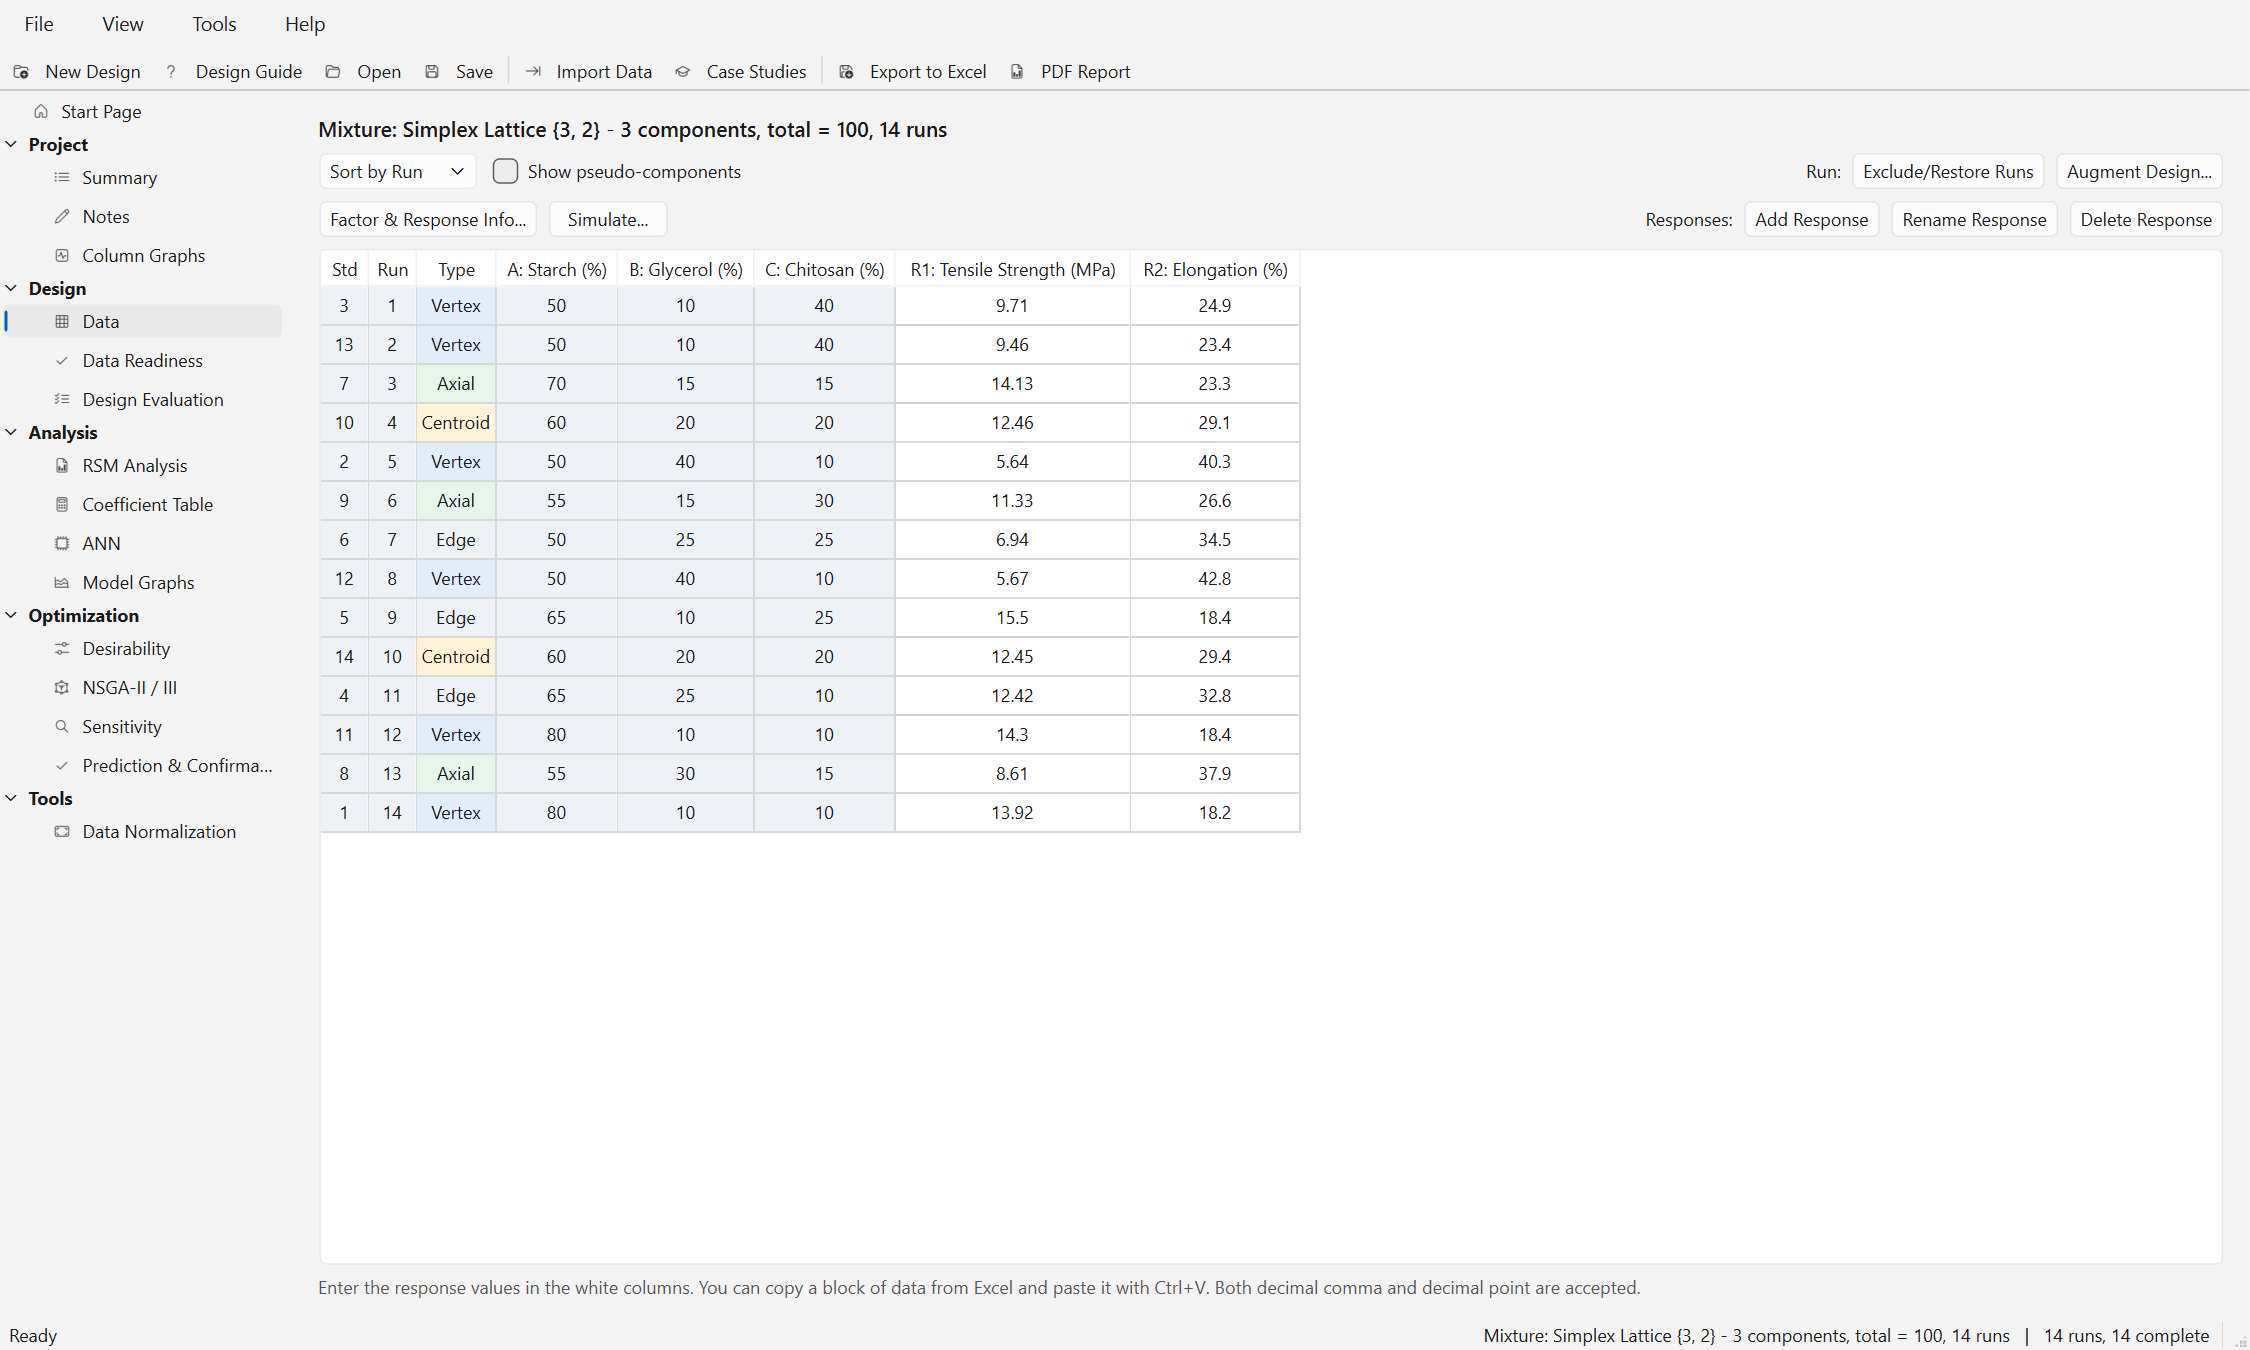
\includegraphics[width=\linewidth]{data_mixture.png}
\caption{Data page of the mixture case ``Edible Film Formulation (Mixture)'': simplex lattice \{3, 2\}, total 100,
14 runs with colour-coded point types.}
\label{fig:ch04-datamix}
\end{figure}

\begin{figure}[htbp]
\centering
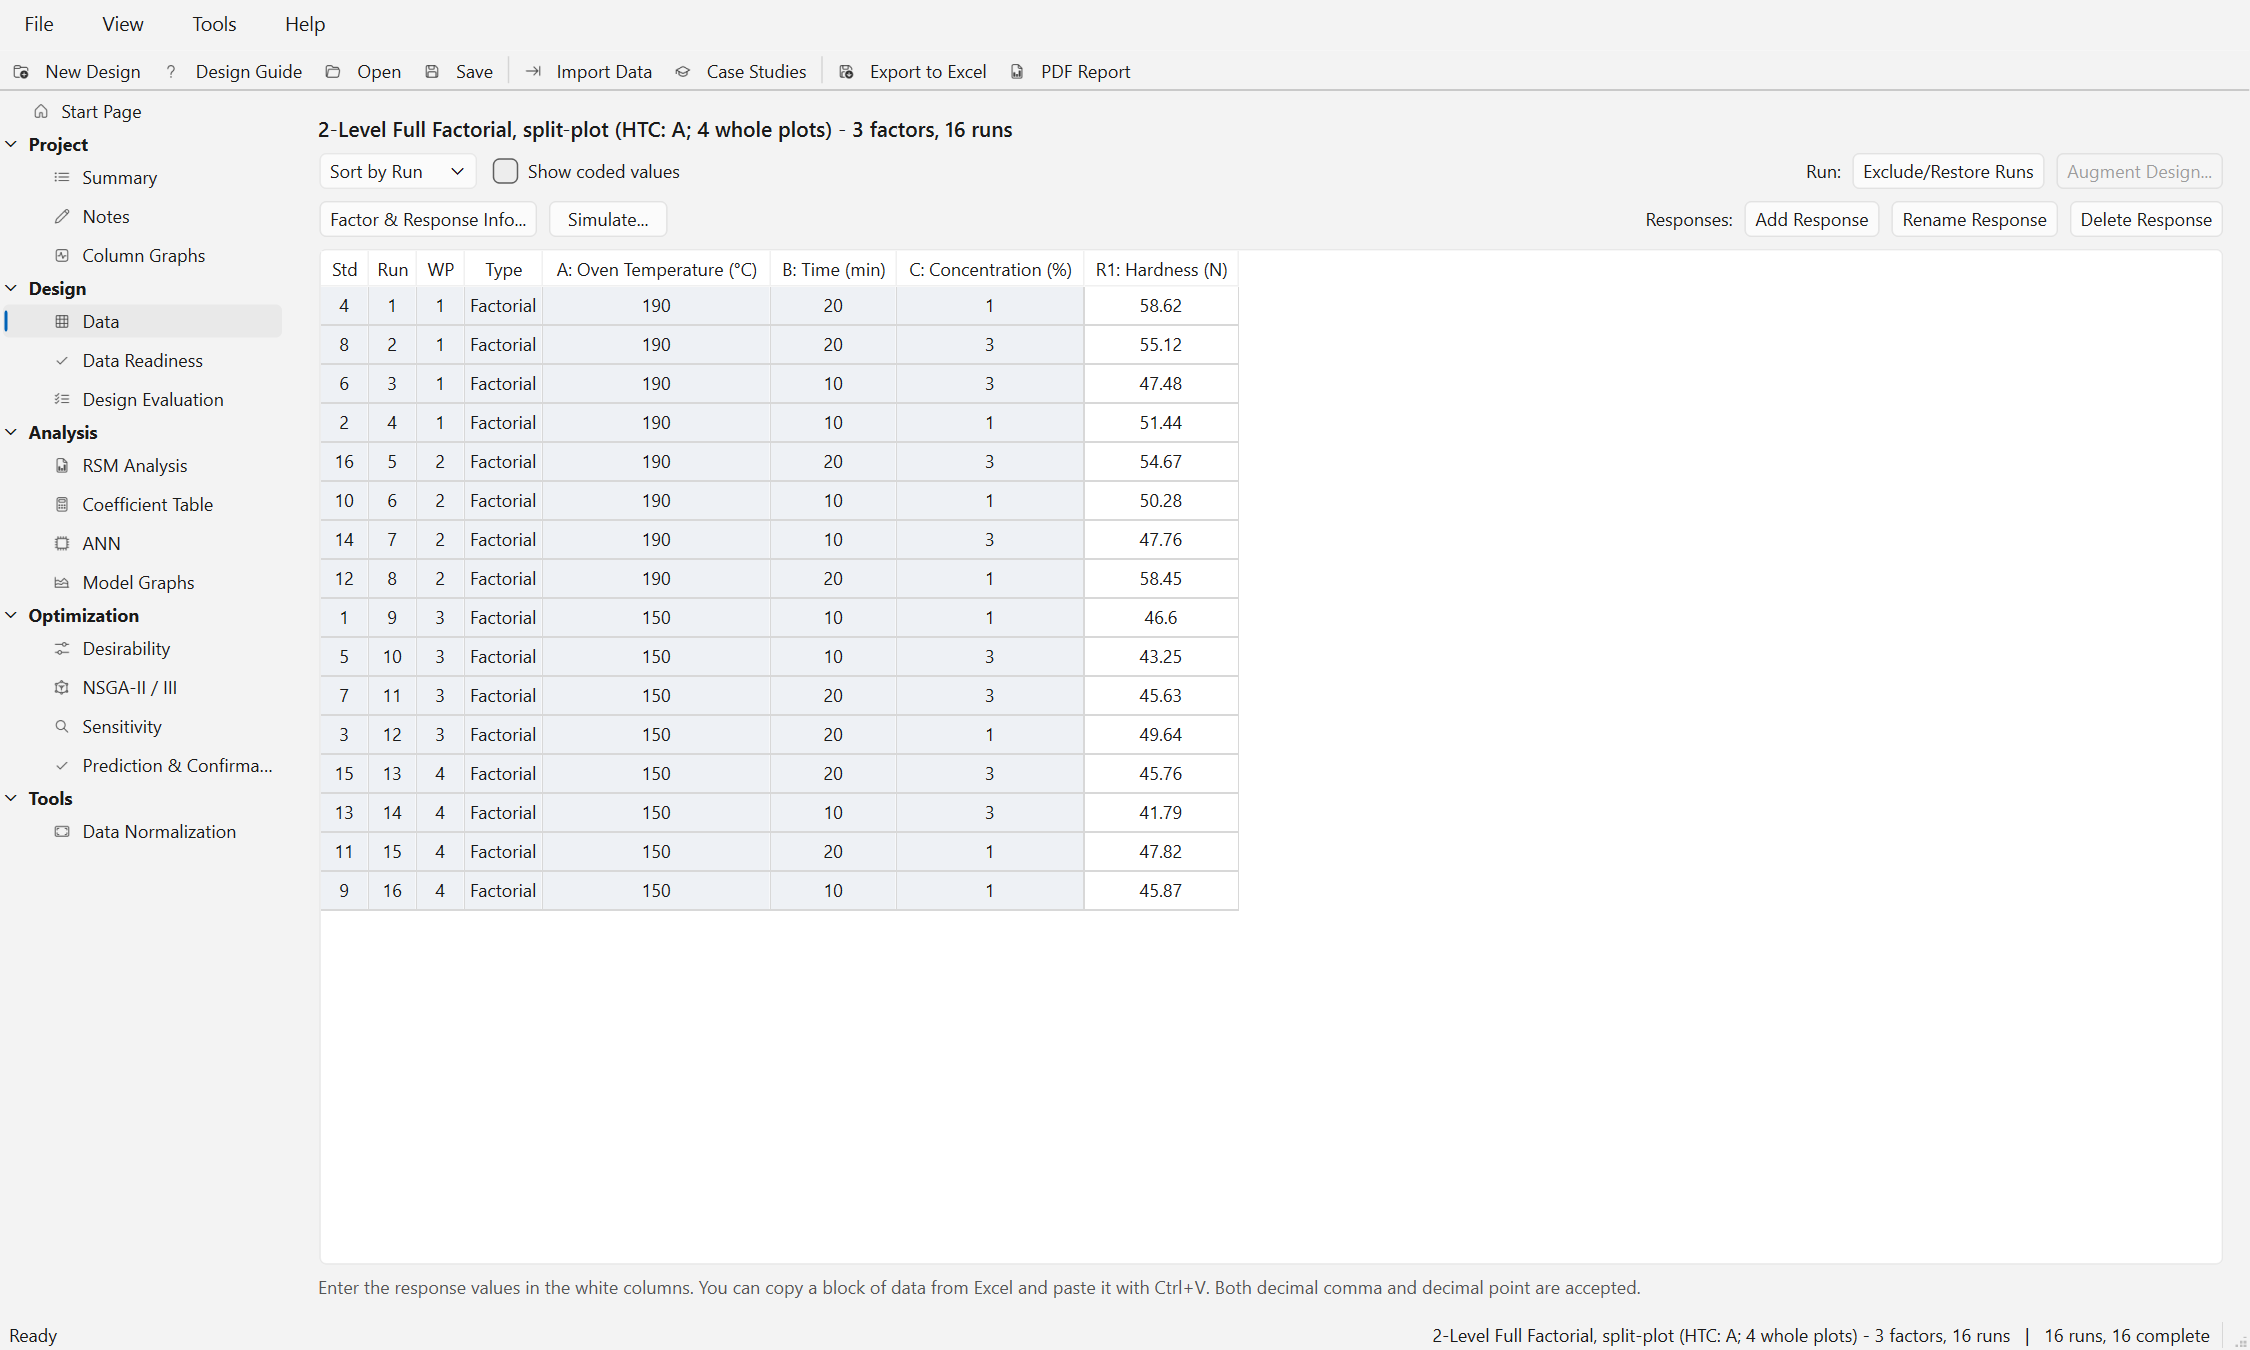
\includegraphics[width=\linewidth]{data_splitplot.png}
\caption{Data page of the split-plot case ``Oven Product Hardness (Split-Plot)'': column WP (whole plot); the
hard-to-change Oven Temperature is constant within each whole plot.}
\label{fig:ch04-datasplit}
\end{figure}

\section{Factor \& Response Info}
\label{sec:ch04-info}

\paragraph{Purpose.} This dialog stores the information about factors and responses that is not part of the design
itself: the standard deviation of each factor for propagation of error (POE), and the type of each response.

\paragraph{How to use.} Click \ui{Factor \& Response Info\dots} on the Data page, edit the tables and click
\ui{Save}.

\begin{table}[htbp]
\centering
\caption{Fields of the Factor \& Response Info dialog.}
\label{tab:ch04-info}
\small
\begin{tabularx}{\linewidth}{@{}p{3.6cm}p{3.6cm}X@{}}
\toprule
Field & Values & Meaning \\
\midrule
\ui{Standard deviation ($\sigma$)} & number $\ge 0$ or empty & Standard deviation of the factor setting in actual
units (how precisely the factor can be held). Empty = controlled precisely. Not available for categorical
factors. \\
\ui{Name}, \ui{Unit} & text & Name and unit of the response. \\
\ui{Type} & Normal (continuous), Binomial (successes out of n), Poisson (counts) & Distribution of the response;
selects the analysis (least squares, logistic regression or Poisson regression). \\
\ui{Trials per run} & number $\ge 1$ & Number of trials $n$ per run for a binomial response (required). \\
\bottomrule
\end{tabularx}
\end{table}

\paragraph{Theory.} POE uses the standard deviations in coded units,
\begin{equation}
\sigma_{\text{coded}} = \frac{\sigma}{s}, \qquad s = \frac{H-L}{2} \ \text{(process factor)}, \quad
s = T - \textstyle\sum_j L_j \ \text{(mixture component)},
\label{eq:ch04-sdcoded}
\end{equation}
where $s$ is the scale of Equation~(\ref{eq:ch03-coding}) or (\ref{eq:ch03-pseudo}). For the extraction case with
$\sigma = 1.0$ \textdegree C, 2.0 min and 0.05 \% the coded values are 0.1, 0.0667 and 0.05. The POE graph and the
POE criterion of the optimization become available once at least one $\sigma$ is entered (Chapters~6 and 8).

A \emph{binomial} response is the number of successes out of $n$ trials per run (for example germinated seeds out of
50) and is analyzed by logistic regression; a \emph{Poisson} response is a count of events and is analyzed by
Poisson regression (Chapter~\ref{chap:5}). Changing the type of a response resets its model specification. Messages: ``The
standard deviation of X is not a number.'' and ``Enter the number of trials per run for X.''. Negative values are
ignored.

\begin{figure}[htbp]
\centering
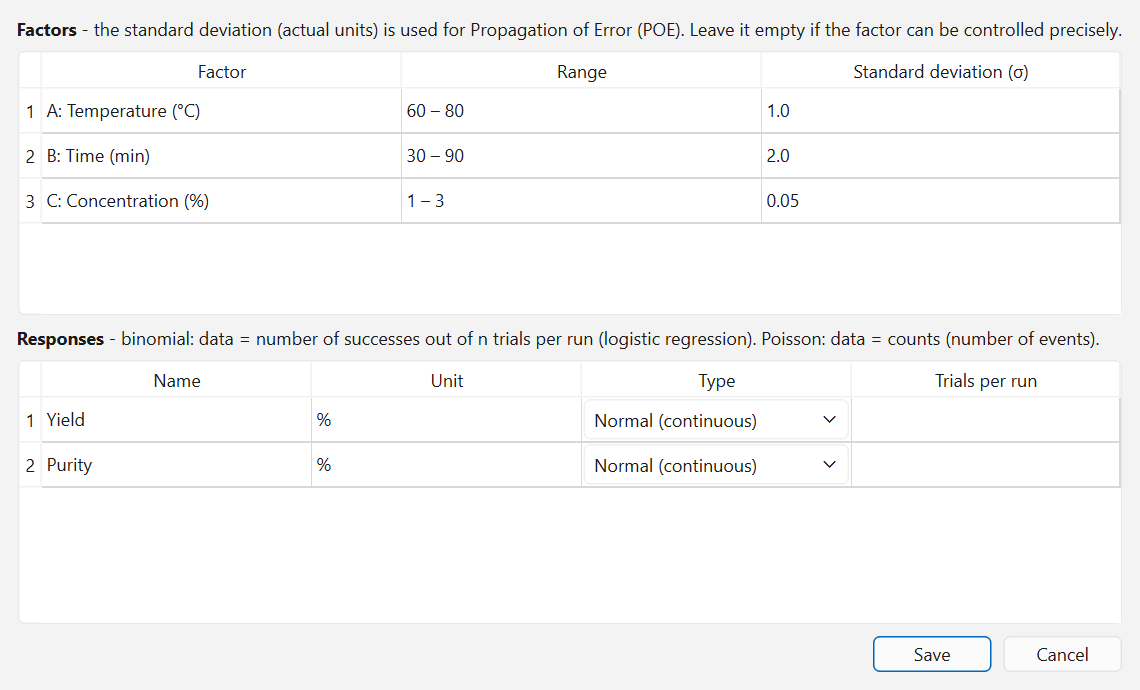
\includegraphics[width=0.75\linewidth]{factor_response_info.png}
\caption{Factor \& Response Info dialog for the extraction case with $\sigma$ = 1.0 \textdegree C (Temperature),
2.0 min (Time) and 0.05 \% (Concentration).}
\label{fig:ch04-info}
\end{figure}

\section{Simulate Response}
\label{sec:ch04-simulate}

\paragraph{Purpose.} \ui{Simulate\dots} fills a response column from an equation plus random noise. It is used for
practice and teaching, for checking how well a design recovers a known model before running it, and for testing the
analysis.

\paragraph{How to use.}
\begin{enumerate}
\item Click \ui{Simulate\dots} on the Data page.
\item Choose the \ui{Response:}, type the \ui{Equation:}, choose the \ui{Factor units:} and set \ui{Noise
($\sigma$):} and \ui{Random seed:}.
\item Tick \ui{Fill empty cells only} to keep values that are already entered.
\item Click \ui{Simulate}. The message ``n response values filled.'' reports the number of cells written.
\end{enumerate}

\begin{table}[htbp]
\centering
\caption{Options of the Simulate Response dialog.}
\label{tab:ch04-simopts}
\small
\begin{tabularx}{\linewidth}{@{}p{3.0cm}p{4.4cm}p{2.4cm}X@{}}
\toprule
Option & Values & Default & Meaning \\
\midrule
\ui{Equation:} & expression (Table~\ref{tab:ch04-simsyntax}) & \texttt{50 + 3*A - 2*B - 4*A**2} & mean response \\
\ui{Factor units:} & Coded factors (-1..+1 / pseudo-components), Actual factors & Coded & scale of the letters \\
\ui{Noise ($\sigma$):} & 0--10\textsuperscript{9} & 1.0 & standard deviation of normal noise \\
\ui{Random seed:} & 0--999\,999 & 1 & same seed = same noise \\
\ui{Fill empty cells only} & check box & off & keep existing values \\
\bottomrule
\end{tabularx}
\end{table}

\paragraph{Equation syntax.} The equation is evaluated safely: only the elements of
Table~\ref{tab:ch04-simsyntax} are allowed.

\begin{table}[htbp]
\centering
\caption{Elements accepted in a simulation equation.}
\label{tab:ch04-simsyntax}
\small
\begin{tabularx}{\linewidth}{@{}p{3.2cm}X@{}}
\toprule
Element & Accepted \\
\midrule
Variables & factor letters A, B, C, \dots{} (I is skipped). Categorical factors take their level index 0, 1, 2, \dots \\
Numbers & with a point as the decimal separator, e.g.\ \texttt{2.5} \\
Operators & \texttt{+ - * /}, power \texttt{**} or \texttt{\textasciicircum}, remainder \texttt{\%} \\
Comparisons & \texttt{< > <= >= == !=}; true = 1, false = 0, e.g.\ \texttt{5*(A > 0)} \\
Functions & \texttt{exp}, \texttt{ln}, \texttt{log} (natural log), \texttt{log10}, \texttt{sqrt}, \texttt{sin},
\texttt{cos}, \texttt{tan}, \texttt{abs} (one argument); \texttt{min(a, b)}, \texttt{max(a, b)} (two arguments) \\
Constants & \texttt{pi}, \texttt{e} \\
Comma & only between the two arguments of \texttt{min} and \texttt{max} \\
\bottomrule
\end{tabularx}
\end{table}

Typical errors: ``Invalid equation: \dots'' (a syntax error; when the text contains a comma the note ``Use a point as
the decimal separator (for example 2.5); commas only separate the arguments of min and max.'' is added), ``Unknown
name 'x'. Use the factor letters (A, B, ...).'', ``Only basic math functions are allowed.'' and ``min() takes 2
arguments.''.

\paragraph{Theory.} Let $f(x)$ be the value of the equation for a run. Depending on the response type:
\begin{align}
\text{Normal:}\quad & y = f(x) + \varepsilon, \quad \varepsilon \sim N(0, \sigma^2), \label{eq:ch04-simnorm}\\
\text{Binomial:}\quad & y \sim \text{Bin}\bigl(n, \operatorname{clip}(f(x), 0, 1)\bigr), \label{eq:ch04-simbin}\\
\text{Poisson:}\quad & y \sim \text{Pois}\bigl(\max(f(x), 0)\bigr). \label{eq:ch04-simpois}
\end{align}
For a binomial response the equation is the success probability, for a Poisson response the mean count. The noise
$\sigma$ applies to normal responses only: for binomial and Poisson responses the field is disabled with the note
``Not used: binomial and Poisson data get their random variation from the distribution.'' Only runs with complete
factor values are filled.

\paragraph{Example.} On a new rotatable CCD with three factors (20 runs), the default equation with coded factors and
$\sigma = 1$ fills all 20 Yield values (``20 response values filled.''). Fitting a quadratic model should then
recover coefficients close to 3, $-2$ and $-4$ for A, B and A\textsuperscript{2}, within about two standard errors
(Design Evaluation gives the standard errors in units of $\sigma$; Section~\ref{sec:ch04-eval}).

\begin{figure}[htbp]
\centering
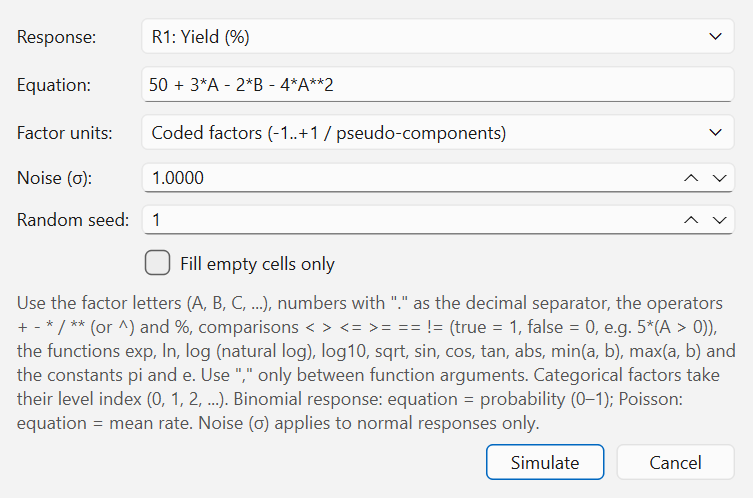
\includegraphics[width=0.6\linewidth]{simulate_dialog.png}
\caption{Simulate Response dialog with the default equation, coded factors, noise $\sigma$ = 1 and seed 1.}
\label{fig:ch04-simulate}
\end{figure}

\section{Data Readiness}
\label{sec:ch04-readiness}

\paragraph{Purpose.} The \ui{Data Readiness} page answers the question ``Are these data good enough to build a
model and to trust an optimum, and if not, what should be done?''. It runs a set of checks on one response, scores
them, lists recommendations (complete the data, or treat the data or the model), and computes suggested additional
runs that can be added to the data sheet with one click. It is especially useful for historical data, which were not
collected according to a design.

\subsection{How to use}
\begin{enumerate}
\item Open \ui{Data Readiness} in the group \ui{Design}.
\item Select the \ui{Response:} and the \ui{Reference model:} (by default the model currently selected for that
response). Click \ui{Reassess} after changing the data elsewhere.
\item Read the score cards, the report on the left and the recommendation list on the right.
\item Select a recommendation and click \ui{Apply Selected Recommendation}. Recommendations marked ``(manual)'' must
be carried out by you; REGEN shows their text.
\item Choose a set of suggested runs under \ui{Suggested runs:}, inspect the table (factor settings in actual units
and, when a model exists, the predicted response) and click \ui{Add Suggested Runs to Data Sheet}. Perform these
experiments, then enter their responses on the Data page.
\end{enumerate}

\subsection{Output}
The six score cards are \ui{Modeling}, \ui{Optimization} and one per category: \ui{Data Completeness \&
Cleanliness}, \ui{Data Structure for Modeling}, \ui{Response \& Model Quality} and \ui{Optimization Readiness}. The
two overall cards show the verdict; the category cards show ``good'' or the number of notes (checks that need
attention or have a problem). The report starts, for projects with more than one response, with a ``Readiness
Summary for All Responses'' table, followed by the verdicts, the number of complete runs and the reference model, one
table per category (Check, Value, Status, Explanation) and the table of recommendations. The status of a check is
\emph{Good}, \emph{Needs attention}, \emph{Problem} or \emph{Info}.

\subsection{Scores and verdicts}
Each check is rated $w = 1$ (Good), $0.5$ (Needs attention) or $0$ (Problem); Info checks are not counted. The score
of a category $c$ with $m_c$ rated checks is
\begin{equation}
S_c = \frac{100}{m_c} \sum_{i \in c} w_i .
\label{eq:ch04-score}
\end{equation}
The modeling score is the mean of the available scores of the categories data, structure and response quality; the
optimization score is the mean of all four category scores (including optimization readiness). The verdict is
\begin{equation}
\text{verdict} = \begin{cases}
\text{``Ready''} & S \ge 85,\\
\text{``Fair - some things need fixing''} & 60 \le S < 85,\\
\text{``Not ready yet''} & S < 60,\\
\text{``Cannot be assessed yet''} & \text{no score.}
\end{cases}
\label{eq:ch04-verdict}
\end{equation}
The thresholds are practical choices, not statistical tests: a score summarizes how many checks pass, it does not
replace reading the individual checks. Recommendations are sorted by the status of their check (problems first)
and, within a status, data completion before treatment.

\subsection{The checks}
Let $N$ be the number of runs with complete factors and a response value (excluded runs count as empty), $p$ the
number of parameters of the reference model and $\nu = N - p$ the residual degrees of freedom. If $N < 3$ the
assessment stops after the first check. Table~\ref{tab:ch04-checks} lists all checks with their rules. Some checks
apply only to normally distributed responses fitted by least squares, some only to process (non-mixture) designs.

\begin{longtable}{@{}p{3.1cm}p{5.6cm}p{6.1cm}@{}}
\caption{Checks of the Data Readiness assessment.}\label{tab:ch04-checks}\\
\toprule
Check & Status rule & Recommendation (action) \\
\midrule
\endfirsthead
\toprule
Check & Status rule & Recommendation (action) \\
\midrule
\endhead
\multicolumn{3}{@{}l}{\emph{Data Completeness \& Cleanliness}}\\
Missing data & Good if no empty factor or response cell; Problem if $N < 3$; else Needs attention &
  Fill in or delete incomplete rows; perform the missing runs (manual). \\
Exact duplicate rows & Needs attention if rows have identical factors \emph{and} response &
  Check them; delete rows that were recorded twice (manual). True replicates almost never give identical values. \\
Constant factors & Problem if a numeric factor has the same value in every run & Remove the factor or add runs at
  other levels (manual). \\
\midrule
\multicolumn{3}{@{}l}{\emph{Data Structure for Modeling}}\\
Runs vs model parameters & Good $\nu \ge 5$; Needs attention $1 \le \nu < 5$; Problem $\nu \le 0$ &
  Add $\max(0, p + 5 - N)$ D-optimal runs. \\
Numeric factor levels (process designs) & Good if every numeric factor has $\ge 3$ distinct levels; otherwise
  Problem if the model has squared terms, else Needs attention & Add $\max(3, 2 \times \text{number of 2-level
  factors})$ D-optimal runs for the quadratic model (``Middle level (curvature)''). \\
Replicates (pure error) & Good if pure-error df $\ge 3$; Needs attention 1--2; Problem 0 & Add 4 replicates at the
  center (mixtures: the centroid of the mixture region). \\
Multicollinearity (max VIF) & Good $\le 5$; Needs attention $\le 10$; Problem $> 10$ & Add
  $\max(4, \lfloor p/2 \rfloor)$ D-optimal runs. \\
High-leverage points & Needs attention if any $h_i > \max(2p/N, 0.5)$ & Add $\max(5, \min(20, \lfloor N/4
  \rfloor))$ gap-filling runs around them. \\
Factor space coverage (process designs) & Good $g \le 0.3$; Needs attention $\le 0.5$; Problem $> 0.5$ & Add
  gap-filling runs. \\
Level balance of \textless factor\textgreater{} (each categorical factor) & Good if the rarest level has $\ge
  \max(3, 0.5 \times \text{most frequent})$ runs; Needs attention if $\ge 2$; else Problem & Add runs at the rarest
  level (manual). \\
\midrule
\multicolumn{3}{@{}l}{\emph{Response \& Model Quality} (normal responses)}\\
Outliers \& influential points & Needs attention if any outlier or Cook's $D > 1$ & Exclude those runs after
  checking them. \\
Response spread \& transform & Needs attention if Box-Cox recommends a transform, none is in use and the residual
  SS drops by $\ge 5\,\%$ & Apply the recommended transform. \\
Constant residual variance ($N > 5$) & Needs attention if Spearman $\rho(|e|, \hat y) > 0$ with $p < 0.05$ & Use a
  ln transform ($y > 0$) or square root. \\
Drift over run order & Needs attention if $DW < 1.4$ or $DW > 2.6$ or the trend has $p < 0.01$ & Check
  calibration and materials, use blocks, randomize (manual). \\
Model fit & Needs attention if lack of fit $p < 0.05$, or Adj R\textsuperscript{2} $-$ Pred R\textsuperscript{2}
  $> 0.2$, or Pred R\textsuperscript{2} $< 0.5$; Problem if Pred R\textsuperscript{2} $< 0$; Info ``R², Adj R², Pred
  R² not available'' for split-plot (REML) responses & Higher-order model; backward elimination with $\alpha = 0.10$
  (split-plot: judge the model by the Wald F tests on the Split-Plot (REML) tab). \\
Signal / noise (needs pure error) & Good $\ge 4$; Needs attention $\ge 2$; Problem $< 2$ & Improve precision,
  average repeats or widen the ranges (manual). \\
Model & Problem if the model cannot be calculated & (error text) \\
\midrule
\multicolumn{3}{@{}l}{\emph{Optimization Readiness}}\\
Model significance & Good if the model $p < 0.05$, else Problem; Info ``no overall model F test (split-plot)'' for
  split-plot (REML) responses & Add runs or widen the factor ranges (manual). \\
Prediction reliability (Pred R\textsuperscript{2}) & Good $\ge 0.7$; Needs attention $\ge 0.4$; Problem $< 0.4$ &
  Add D-optimal runs; with $N \ge 30$ also ``try an ANN'' (manual). \\
Optimum location & Needs attention if a process factor of the optimum lies within 2\,\% of its range from a bound
  & Extend the range in that direction (steepest ascent) (manual). \\
Data support around the optimum & Needs attention if $d > 0.2$ or the CI half-width exceeds 10\,\% of the response
  range & 4 confirmation runs around the optimum. \\
\bottomrule
\end{longtable}

\subsection{Formulas as implemented}
\paragraph{Outliers.} A run is an outlier if its externally studentized residual exceeds the Bonferroni limit,
\begin{equation}
|t_i| > t_{1 - 0.05/(2N),\; \nu - 1},
\label{eq:ch04-bonf}
\end{equation}
and it is influential if Cook's distance $D_i > 1$ \citep{cook1977}. Both are explained in Chapter~\ref{chap:5}.

\paragraph{Box-Cox.} The residual sum of squares of the scaled power transform
$w = (y^\lambda - 1)/(\lambda \dot y^{\lambda-1})$ ($w = \dot y \ln y$ for $\lambda = 0$, $\dot y$ = geometric mean)
is computed for 121 values $\lambda \in [-3, 3]$ \citep{boxcox1964}. The 95\,\% interval contains all $\lambda$ with
$\ln SS(\lambda) \le \ln SS_{\min} + \ln(1 + t^2_{0.975,\nu}/\nu)$. No transform is recommended if $\lambda = 1$
lies inside; otherwise the first of square root ($\lambda = 0.5$), ln (0) and inverse ($-1$) inside the interval, or
the power transform with the best $\lambda$. The gain is $1 - \exp(\ln SS_{\min} - \ln SS(1))$.

\paragraph{Constant variance and drift.} The variance check uses the Spearman rank correlation \citep{spearman1904}
between $|e_i|$ and $\hat y_i$. For drift the residuals are sorted by run order and the Durbin--Watson statistic
\citep{durbin1950}
\begin{equation}
DW = \frac{\sum_{t=2}^{N} (e_t - e_{t-1})^2}{\sum_{t=1}^{N} e_t^2}
\label{eq:ch04-dw}
\end{equation}
is computed ($DW \approx 2$ for independent residuals); the trend is the Spearman correlation between run order and
residual.

\paragraph{Signal to noise.} With $SS_{PE}$ and $df_{PE}$ the pure-error sum of squares and degrees of freedom of
replicated points (identical coded settings, same block),
\begin{equation}
\text{SNR} = \frac{\operatorname{SD}(y)}{\sqrt{SS_{PE}/df_{PE}}} .
\label{eq:ch04-snr}
\end{equation}

\paragraph{Coverage gap.} Numeric factors are scaled to $[0,1]$ by their coded bounds ($u$), 3000 points $u_r$ are
drawn from the design region (respecting constraints), and
\begin{equation}
g = \frac{1}{\sqrt{k_{\text{num}}}}\, \max_r \min_i \lVert u_r - u_i \rVert ,
\label{eq:ch04-gap}
\end{equation}
the largest distance from a point of the region to the nearest run, relative to the diagonal of the unit cube.

\paragraph{Optimum.} The optimum is the first solution of the last desirability optimization if one exists (``last
optimization result''), otherwise the best of 4000 random region points according to the goal of the response in the
optimization criteria (default maximize: ``Model-predicted maximum''). The distance $d$ to the nearest run is
computed like Equation~(\ref{eq:ch04-gap}); $h$ is the half-width of the model's 95\,\% confidence interval at the
optimum.

\subsection{Suggested runs}
\label{sec:ch04-suggest}
\begin{itemize}
\item \emph{D-optimal (adds model information)} and \emph{Middle level (curvature)}: 3000 random points of the region
are the candidates. Runs are added one at a time, each time the candidate with the largest prediction variance
$x^\top M^{-1} x$, with $M = X_e^\top X_e + 10^{-6} I$ for the existing runs, updated by Sherman--Morrison:
\begin{equation}
M^{-1} \leftarrow M^{-1} - \frac{M^{-1} x x^\top M^{-1}}{1 + x^\top M^{-1} x}.
\label{eq:ch04-sm}
\end{equation}
Adding the point of largest prediction variance gives the largest increase of $\det M$, so this is a greedy
D-optimal augmentation \citep{goos2011}.
\item \emph{Factor space gap filling}: from 3000 region points, repeatedly the point farthest from all existing and
already chosen runs (maximin), with numeric factors scaled to $[0,1]$.
\item \emph{Replicates (pure error)}: 4 copies of the center point (mixtures: the overall centroid of the mixture
region; categorical factors from the run nearest the center).
\item \emph{Confirmation around the optimum}: the optimum itself and up to three random region points within a
scaled distance of 0.15 from it, with the same categorical levels.
\end{itemize}
The confirmation ``Add n runs (\textless label\textgreater) to the data sheet? Their responses are empty and must be
entered after the experiments are run.'' precedes the addition. The runs are added with the point types D-optimal,
Mid-level, Replicate, Space-filling or Confirmation, at the end of the run order; in split-plot designs each new run
forms its own whole plot. The suggestions use fixed random seeds, so a reassessment of the same data gives the same
suggestions.

\paragraph{Apply Selected Recommendation.} Depending on the recommendation: suggested runs are added (as above); runs
are excluded after the question ``Ignore runs \dots{} in the analysis? The data are not deleted and can be restored on
the Data or Diagnostics page.''; or the model specification of the response is changed (transform, higher model
order, or backward elimination at $\alpha_{\text{out}} = 0.10$) and the page is reassessed.

\subsection{Examples}
\paragraph{A good designed experiment.} For the BBD extraction case, response Yield, quadratic reference model
(Figure~\ref{fig:ch04-readiness}), the modeling score is 94 and the optimization score 96, both ``Ready''. All
structure checks are Good (17 runs, 10 parameters, residual df 7; 3 levels per factor; pure-error df 4; max VIF 1.01;
largest gap 0.27). Two checks need attention: ``0 outliers, 2 Cook's $>$ 1'' (runs 1 and 7) and the model fit with
lack-of-fit $p = 0.030$; the recommendations are to check runs 1 and 7 and to try a higher-order model, a transform
or an ANN. The optimum predicted by the model (Temperature 75.5 \textdegree C, Time 86.1 min, Concentration 2.30 \%)
lies 0.16 from the nearest run with a CI of $\pm 0.99$ (7\,\% of the range), so the only suggested runs are four
confirmation runs. Purity scores 100 and 97; its optimum is less well supported (CI 10\,\% of the range).

\begin{figure}[htbp]
\centering
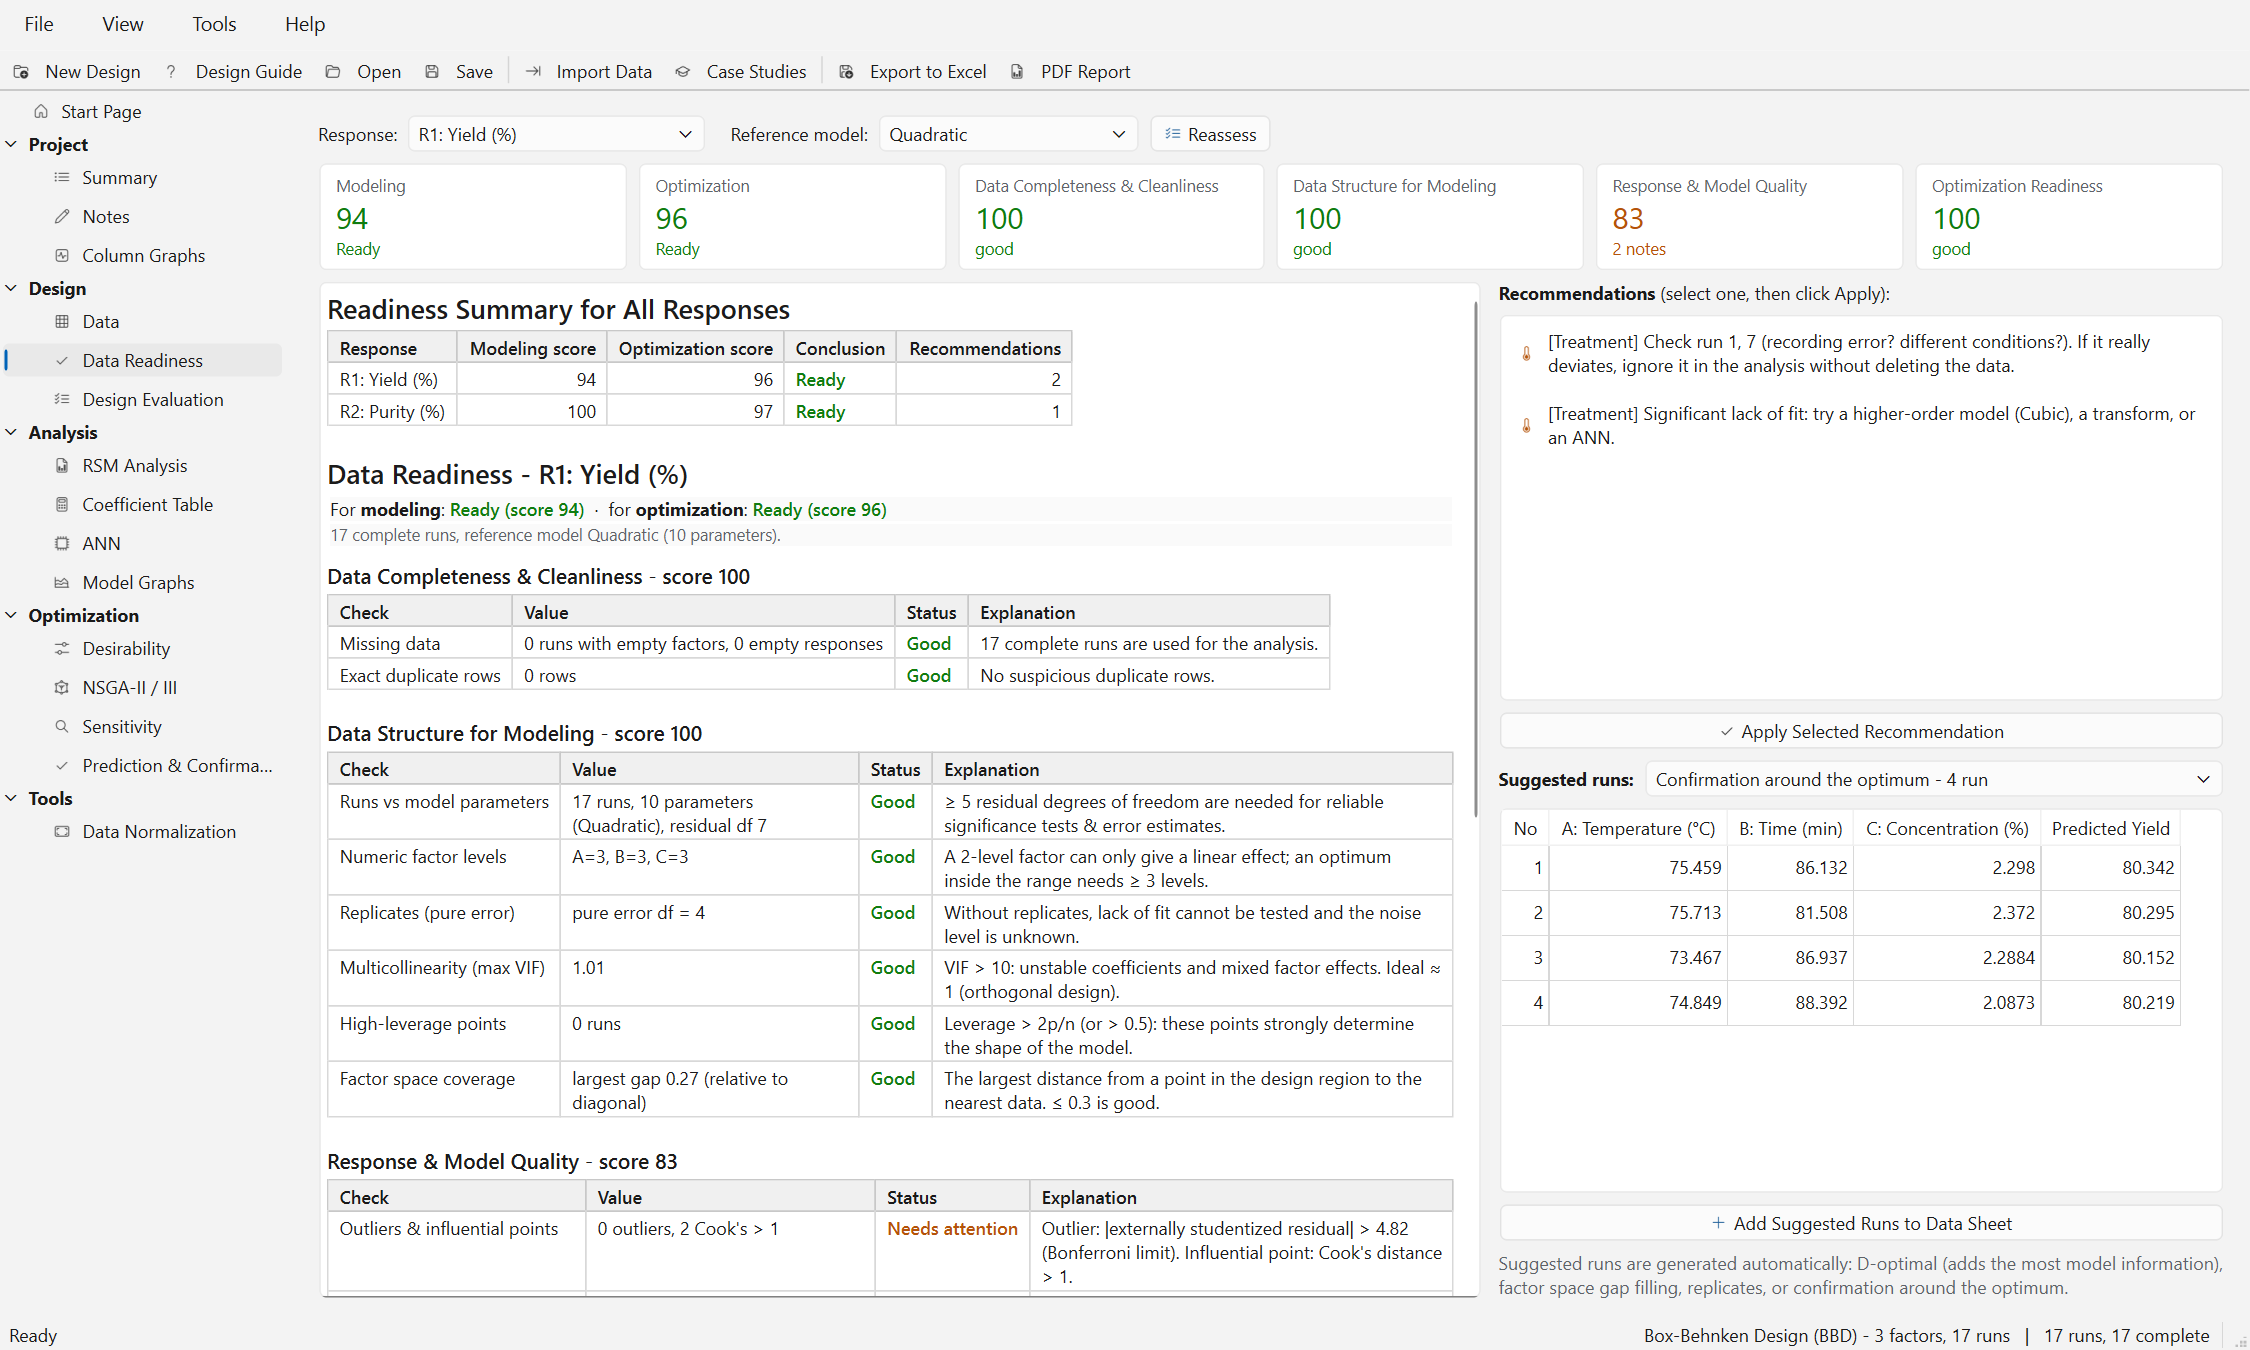
\includegraphics[width=\linewidth]{readiness.png}
\caption{Data Readiness of the BBD extraction case, response Yield: Modeling 94 and Optimization 96 (Ready), two
notes in Response \& Model Quality, and four suggested confirmation runs around the optimum.}
\label{fig:ch04-readiness}
\end{figure}

\paragraph{Historical data for an ANN.} The dye adsorption case (40 Latin hypercube runs, quadratic reference model
with 15 parameters; Figure~\ref{fig:ch04-readinessdye}) scores 82 for modeling and 77 for optimization (``Fair -
some things need fixing''). The category scores follow Equation~(\ref{eq:ch04-score}): Data Structure 75
($[1 + 1 + 0 + 1 + 0.5 + 1]/6$, with ``pure error df = 0'' a Problem and one high-leverage run), Response \& Model
Quality 70 and Optimization Readiness 62.5 (shown as 62). The findings: no replicates; Box-Cox $\lambda = 0.00$ (CI
$-0.15$ to $0.15$) with an 87\,\% drop of the residual SS, so a ln transform is recommended; Durbin--Watson 1.36
(possible drift); Pred R\textsuperscript{2} 0.562; the predicted optimum has Adsorbent Dose 0.53 g/L, within 2\,\%
of its lower limit 0.5, and a CI of $\pm 17.8$ (32\,\% of the range). Suggested runs: 4 replicates at pH 6, dose
2.25 g/L, time 65 min, concentration 110 mg/L; 10 gap-filling runs; 7 D-optimal runs; 4 confirmation runs. Because
$N \ge 30$ and Pred R\textsuperscript{2} is low, an ANN is also suggested. A sensible order of action is: add the
replicates (they also make the ANN diagnosis possible), apply the ln transform, reassess, then compare RSM with an
ANN (Chapter~\ref{chap:7}).

\begin{figure}[htbp]
\centering
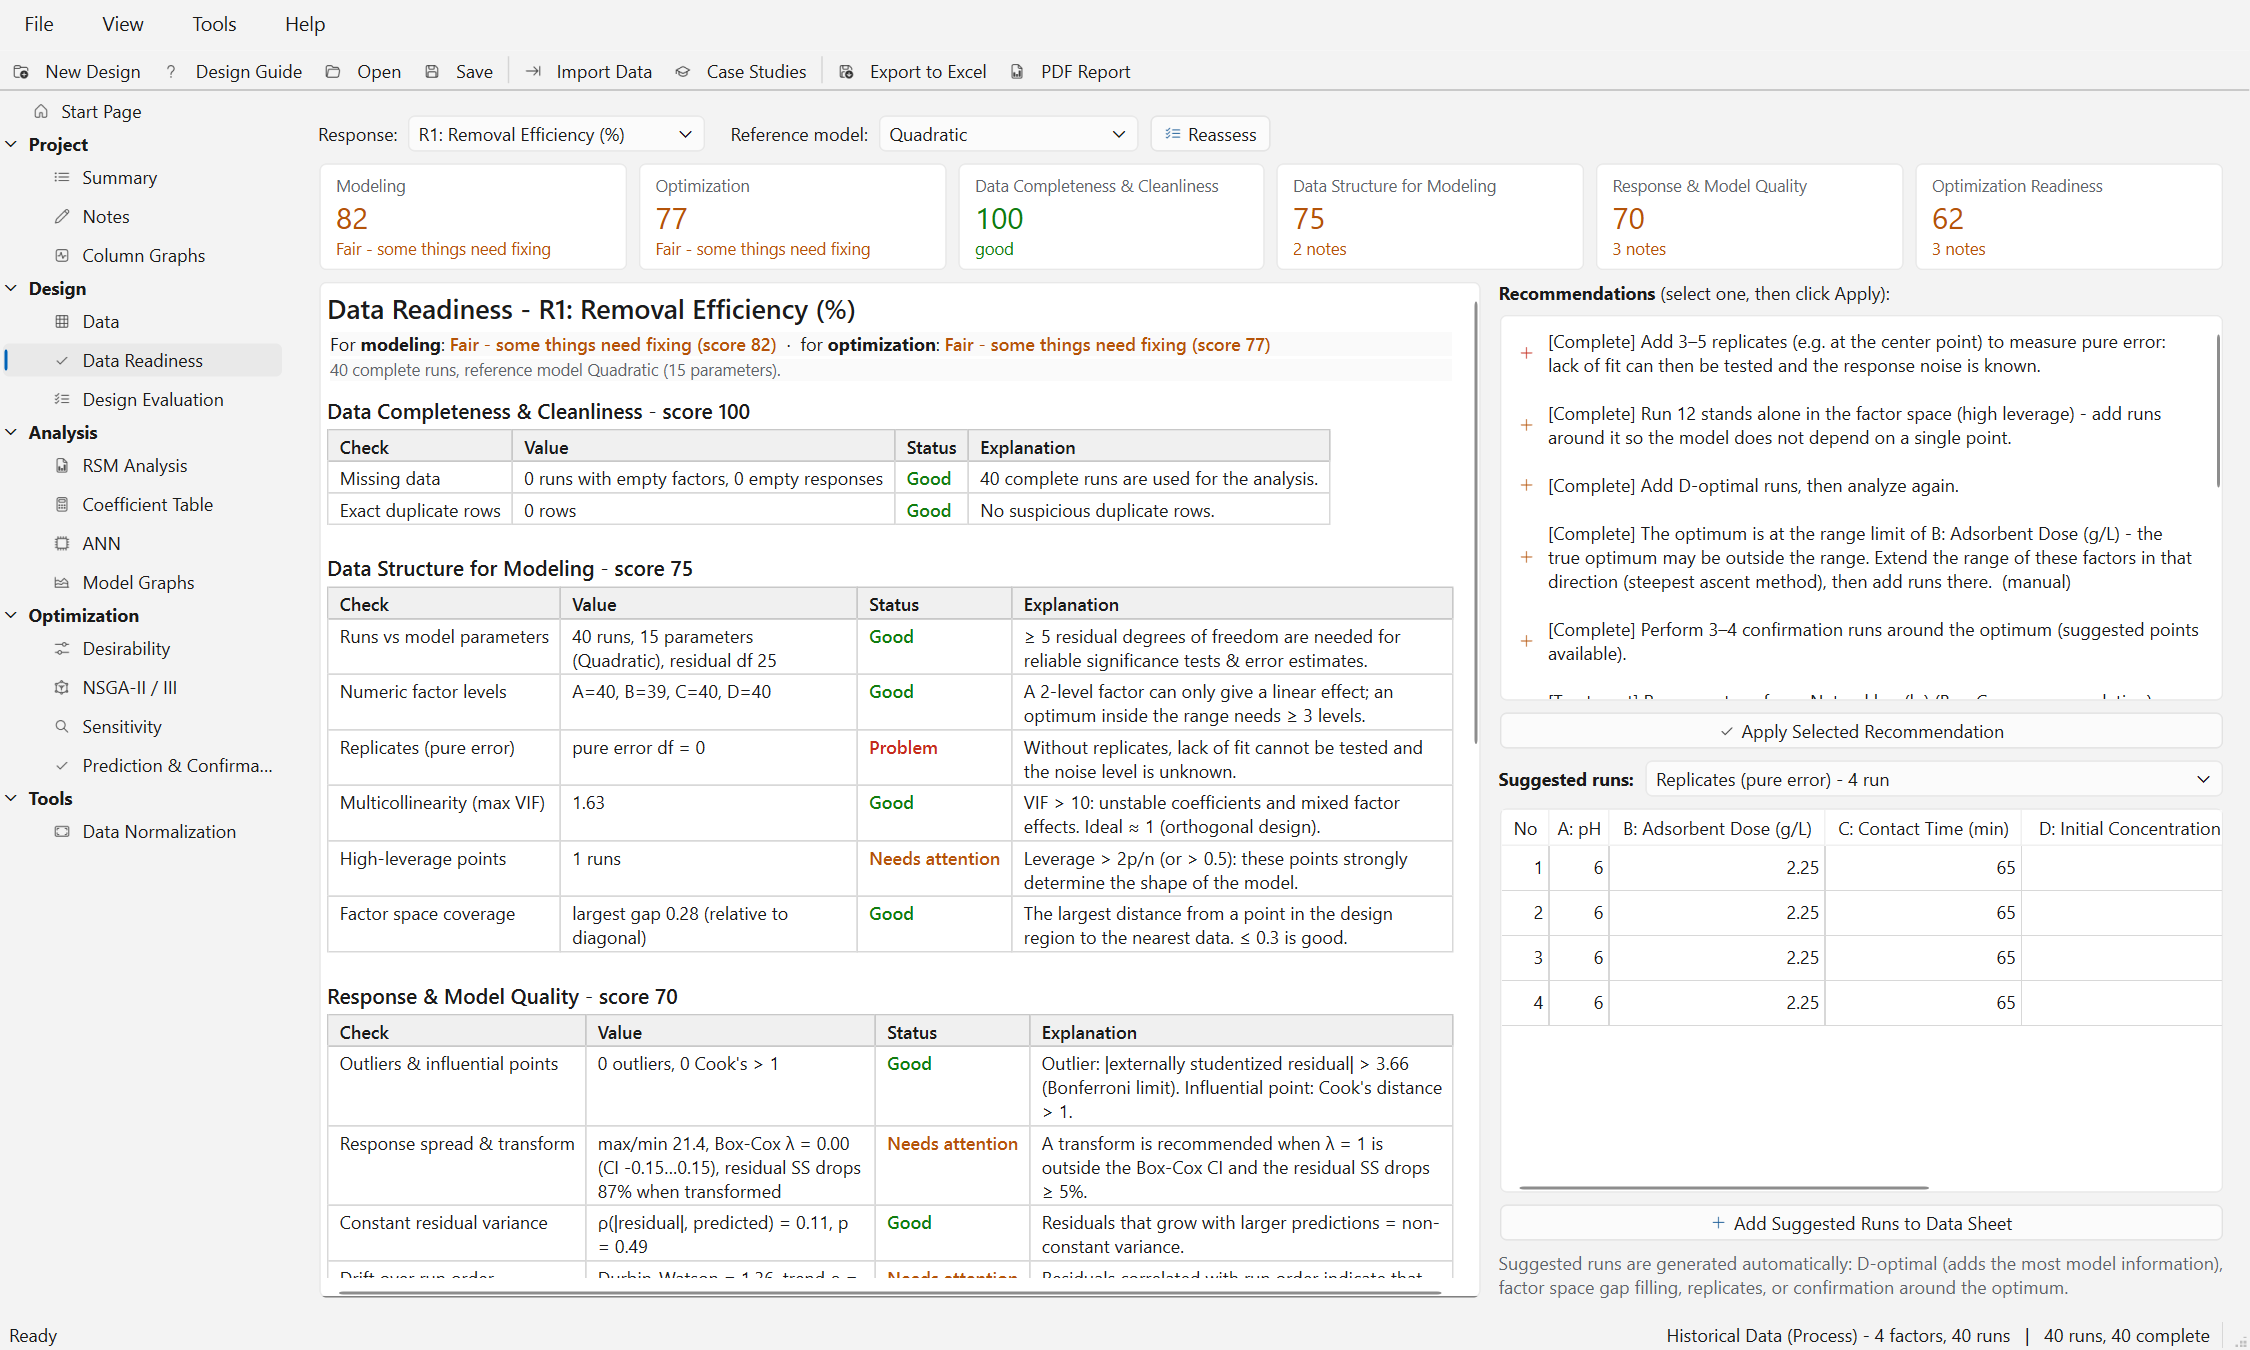
\includegraphics[width=\linewidth]{readiness_dye.png}
\caption{Data Readiness of the dye adsorption case (40 historical runs): Modeling 82 and Optimization 77, ``Fair -
some things need fixing''; the suggested runs show four replicates at the center.}
\label{fig:ch04-readinessdye}
\end{figure}

\paragraph{An unreplicated screening factorial.} For the 2\textsuperscript{4} fermentation case (Biomass, 2FI
model) the scores are 89 and 85. The structure checks flag 2 levels per factor (Needs attention, because the 2FI
model has no squared terms), pure-error df 0 (Problem) and a coverage gap of 0.48 (the interior of the cube holds no
runs). These are the expected limits of a screening design, not errors; the suggested middle-level runs, center
replicates and gap-filling runs are exactly the next stage of a sequential experiment (compare the augmentation to a
CCD in Chapter~\ref{chap:3}).

\paragraph{Limitations.} The assessment refers to one response and one reference model at a time; for GLM
(binomial, Poisson) and split-plot (REML) responses only part of the checks apply. For split-plot responses the
checks ``Model fit'' and ``Model significance'' are Info checks (not counted in the scores): R², adjusted and
predicted R² and an overall model F test are not defined for the REML model, which is judged by the Wald F tests of
its terms on the \ui{Split-Plot (REML)} tab of the RSM Analysis page (Chapter~\ref{chap:5}). Passing all checks does not prove that a model is right:
confirmation runs remain the final test.

\section{Design Evaluation}
\label{sec:ch04-eval}

\paragraph{Purpose.} \ui{Design Evaluation} judges the design matrix itself: how many degrees of freedom are left,
which terms are aliased, how precisely each coefficient can be estimated, how likely an effect of a given size is to
be detected (power), how correlated the model terms are and how the prediction variance is distributed over the
region. No response data are needed, so the page can be used before the experiment, to compare candidate designs, or
afterwards to assess historical data.

\paragraph{How to use.} Open \ui{Design Evaluation} in the group \ui{Design}, select the \ui{Model to evaluate:},
enter the effect size to detect (\ui{Signal $\Delta$:}) and the expected noise (\ui{Noise $\sigma$:}), choose
\ui{$\alpha$:} and the \ui{Graph:}. All runs with complete factor values are used, except excluded runs; blocks are
included in the model when the design has more than one block.

\begin{table}[htbp]
\centering
\caption{Options of the Design Evaluation page.}
\label{tab:ch04-evalopts}
\small
\begin{tabularx}{\linewidth}{@{}p{3.2cm}p{5.2cm}p{2.0cm}X@{}}
\toprule
Option & Values & Default & Meaning \\
\midrule
\ui{Model to evaluate:} & model orders of the design & design default & model whose coefficients are judged \\
\ui{Signal $\Delta$:} & 0.01--10\textsuperscript{6} & 2 & response difference between low and high level to detect \\
\ui{Noise $\sigma$:} & 0.0001--10\textsuperscript{6} & 1 & standard deviation of the response noise \\
\ui{$\alpha$:} & 0.01, 0.05, 0.1 & 0.05 & significance level of the tests \\
\ui{Graph:} & Fraction of Design Space (FDS), Prediction Std. Error Contour, Leverage per Run, Coefficient
Correlation Matrix, Pearson r Between Terms & FDS & plot on the right \\
\bottomrule
\end{tabularx}
\end{table}

Only the ratio $\Delta/\sigma$ matters for the power; $\sigma$ also scales the standard errors in the plots. A
practical choice is $\sigma$ = the expected repeatability of the measurement and $\Delta$ = the smallest change of
the response that matters in practice.

\subsection{Report}
\begin{itemize}
\item \textbf{Degrees of Freedom}: number of runs $n$, model coefficients $p$ (including intercept and block
columns), residual $n - p$, lack of fit and pure error. Notes appear when there is no residual df, fewer than 3
pure-error df or fewer than 3 lack-of-fit df. The box recalls the recommendation: at least 3 lack-of-fit df, 4
pure-error df and 5 residual df.
\item \textbf{Terms that cannot be estimated (aliased)}: model columns that are linear combinations of earlier
columns (QR rank check with tolerance $10^{-8}\max(1, \max|X|)\max(n, p)$); they are dropped.
\item \textbf{Coefficients}: per term the standard error (in units of $\sigma$), VIF, $R_i^2$ and power (green when
$\ge 80\,\%$).
\item \textbf{Alias Structure}: for each model term, the higher-order terms that bias its estimate.
\item \textbf{Matrix Measures}: condition number, determinant and trace of $(X^\top X)^{-1}$, D-, A- and
G-efficiency, average prediction variance I and $n \cdot I$, maximum and minimum prediction variance, maximum and
mean leverage.
\item \textbf{Correlation Between Terms (Pearson r)}: up to 10 pairs with $|r| \ge 0.3$ (red when $|r| \ge 0.7$), or
the note that no pair reaches 0.3, and the maximum $|r|$.
\item \textbf{Leverage}: mean and maximum.
\end{itemize}

\subsection{Theory as implemented}
Let $X$ be the $n \times p$ model matrix in coded units: intercept (omitted for Scheff\'e mixture models), block
columns (sum-to-zero coding), model terms (categorical factors effect coded), aliased columns removed. Let
$C = (X^\top X)^{+}$.

\paragraph{Standard error, VIF and leverage.}
\begin{equation}
SE_j = \sqrt{C_{jj}} \ (\times\sigma), \qquad
\text{VIF}_j = C_{jj} \sum_{i} (x_{ij} - \bar x_j)^2, \qquad R_j^2 = 1 - \frac{1}{\text{VIF}_j}, \qquad
h_i = x_i^\top C\, x_i .
\label{eq:ch04-se}
\end{equation}
VIF = 1 means the term is orthogonal to all others; VIF $> 10$ indicates strong collinearity \citep{belsley1980}.
VIF is not computed for the intercept nor for mixture models without intercept (the Scheff\'e terms are correlated
by construction). The mean leverage is $p/n$; a leverage close to 1 means the run alone determines part of the
model.

\paragraph{Degrees of freedom.} Pure-error df $= n - $ the number of distinct points (same block, coordinates rounded
to 6 decimals); lack-of-fit df $= (n - p) - df_{PE}$.

\paragraph{Power.} Each non-intercept coefficient is tested with a two-sided $t$ test with $n - p$ df. An effect
$\Delta$ between the low ($-1$) and high ($+1$) level corresponds to a coefficient $\beta = \Delta/2$; the
noncentrality parameter and the power are \citep{montgomery2017}
\begin{equation}
\lambda_j = \frac{\Delta/2}{\sigma\, SE_j}, \qquad
\text{Power}_j = 1 - F_{t'}\bigl(t_c;\, n-p,\, \lambda_j\bigr) + F_{t'}\bigl(-t_c;\, n-p,\, \lambda_j\bigr),
\qquad t_c = t_{1-\alpha/2,\, n-p},
\label{eq:ch04-power}
\end{equation}
where $F_{t'}$ is the cumulative distribution of the noncentral $t$ distribution. For a squared term the same
$\beta = \Delta/2$ is used. For mixture terms the ``low to high'' interpretation does not apply directly; use the
power only to compare mixture designs with each other.

\paragraph{Alias matrix.} The potential terms are those of the next higher model order (linear $\rightarrow$ 2FI,
2FI $\rightarrow$ 3FI, quadratic and special cubic $\rightarrow$ cubic) that are not in the model. With $X_2$ their
columns,
\begin{equation}
A = (X^\top X)^{+} X^\top X_2, \qquad E(\hat\beta) = \beta + A\,\beta_2 ,
\label{eq:ch04-alias}
\end{equation}
and every entry $|A_{jl}| > 10^{-6}$ is listed \citep{myers2016}. No alias table is shown for combined
mixture--process models.

\paragraph{Prediction variance and FDS.} The variance of the predicted mean at a point $x$ is
$v(x) = f(x)^\top C\, f(x)$, in units of $\sigma^2$; its square root is the prediction standard error. The Fraction of
Design Space plot \citep{myers2016} draws 4000 random points of the region (uniform in the box, Dirichlet for
mixtures, constraints respected), sorts their standard errors and plots them against the fraction of the region;
dotted lines and labels mark the standard error at 50\,\% and 80\,\% of the region. A low, flat curve is good.

\paragraph{Matrix measures.} With 3000 random region points $\mathcal{R}$ for the average prediction variance:
\begin{align}
\text{D-efficiency} &= 100\,\frac{|X^\top X|^{1/p}}{n}, &
\text{A-efficiency} &= 100\,\frac{p}{n \operatorname{tr} C}, \label{eq:ch04-deff}\\
\text{G-efficiency} &= 100\,\frac{p_m}{n \max_{x \in \mathcal{G}} v(x)}, &
I &= \operatorname{mean}_{x \in \mathcal{R}} v(x), \quad n \cdot I . \label{eq:ch04-geff}
\end{align}
For the G-efficiency, $p_m$ counts the model columns only (block columns are left out of both $p_m$ and $v(x)$), and
the maximum is taken over the set $\mathcal{G}$ of the design points, the corners of the region (the vertices for
mixtures and for constrained process regions, crossed with all levels of the categorical factors) and the 3000
random points. Because the design points and the corners are included, the worst prediction variance is not missed
and the G-efficiency does not exceed 100\,\% (for example, a 2\textsuperscript{7-4} design with its fold-over
gives 100\,\%). The page describes it as ``worst prediction variance in the design region (design points, corners or
vertices, random points); block terms excluded''. The condition number is $\lambda_{\max}/\lambda_{\min}$ of $X^\top X$ (1 = orthogonal, $> 100$ multicollinear,
$> 1000$ severe). The efficiencies are relative to an ideal orthogonal design with coded levels $\pm 1$ and are
computed in coded units; they are meant for comparing designs, also with different numbers of runs, or for assessing
historical data. Three limitations should be kept in mind: (1) for mixtures the pseudo-components range from 0 to 1,
so the efficiencies are much lower by construction and are only comparable between mixture designs; (2) with more
than 12 process factors no corners are used, and when the corners crossed with the categorical levels exceed 4096
combinations a random subset of 4096 is used, so the maximum of $v(x)$ can then be slightly underestimated; (3) for a
design with points outside the $\pm 1$ cube (a rotatable CCD) the average $I$ and the corners refer to the cube,
while the axial design points enter only the maximum of the G-efficiency.

\paragraph{Graphs.} \ui{Prediction Std. Error Contour}: contours of the prediction standard error over the first two
numeric factors (or a ternary plot of the first three components), other numeric factors at 0 (mixtures: the mean of
the design), categorical factors at their first level, with the design points; messages ``At least 2 numeric
factors (or 3 components) are required.'' and ``The slice is empty.''. \ui{Leverage per Run}: leverage in run order
with the reference line $2p/n$. \ui{Coefficient Correlation Matrix}: $C_{ab}/\sqrt{C_{aa}C_{bb}}$, the correlation
between the coefficient estimates. \ui{Pearson r Between Terms}: correlation between the model columns. Both heat
maps print the values when there are at most 16 terms.

\paragraph{Data export.} Every plot has \ui{Copy data} and \ui{Export data\dots} in its toolbar and right-click menu
(the FDS curve, the contour grid, the leverages or the matrices); the report has \ui{Export all tables\dots} in its
right-click menu.

\subsection{Examples}
\paragraph{BBD extraction case.} With the quadratic model, $\Delta = 2$, $\sigma = 1$, $\alpha = 0.05$
(Figure~\ref{fig:ch04-eval}): 17 runs, 10 coefficients, 7 residual df, 3 lack-of-fit df and 4 pure-error df (from
the 5 center points). The standard errors are 0.3536 for A, B, C, 0.5 for the interactions and 0.4873 for the
squares; the VIFs are 1 and 1.006. The power is 68.1\,\% for the main effects, 40.8\,\% for the interactions and
42.5\,\% for the squared terms, all below 80\,\%: an effect of two noise standard deviations would often be missed.
Raising the signal to $\Delta = 3$ raises all powers; in practice, replicates or a larger design would be needed for
small effects. The alias table shows that A is biased by $+0.5\,\text{AB}^2 + 0.5\,\text{AC}^2 + 1\,\text{A}^3$ if
cubic terms are active. Matrix measures: condition number 11.53, D-efficiency 34.0\,\%, A-efficiency 28.9\,\%,
G-efficiency 43.2\,\% (the largest prediction variance, $1.36\sigma^2$, is at the corners of the cube, where a BBD
has no runs), I = 0.340, maximum leverage 0.75, mean 0.588. The FDS curve gives a standard error of
$0.548\sigma$ at 50\,\% and $0.668\sigma$ at 80\,\% of the region.

\begin{figure}[htbp]
\centering
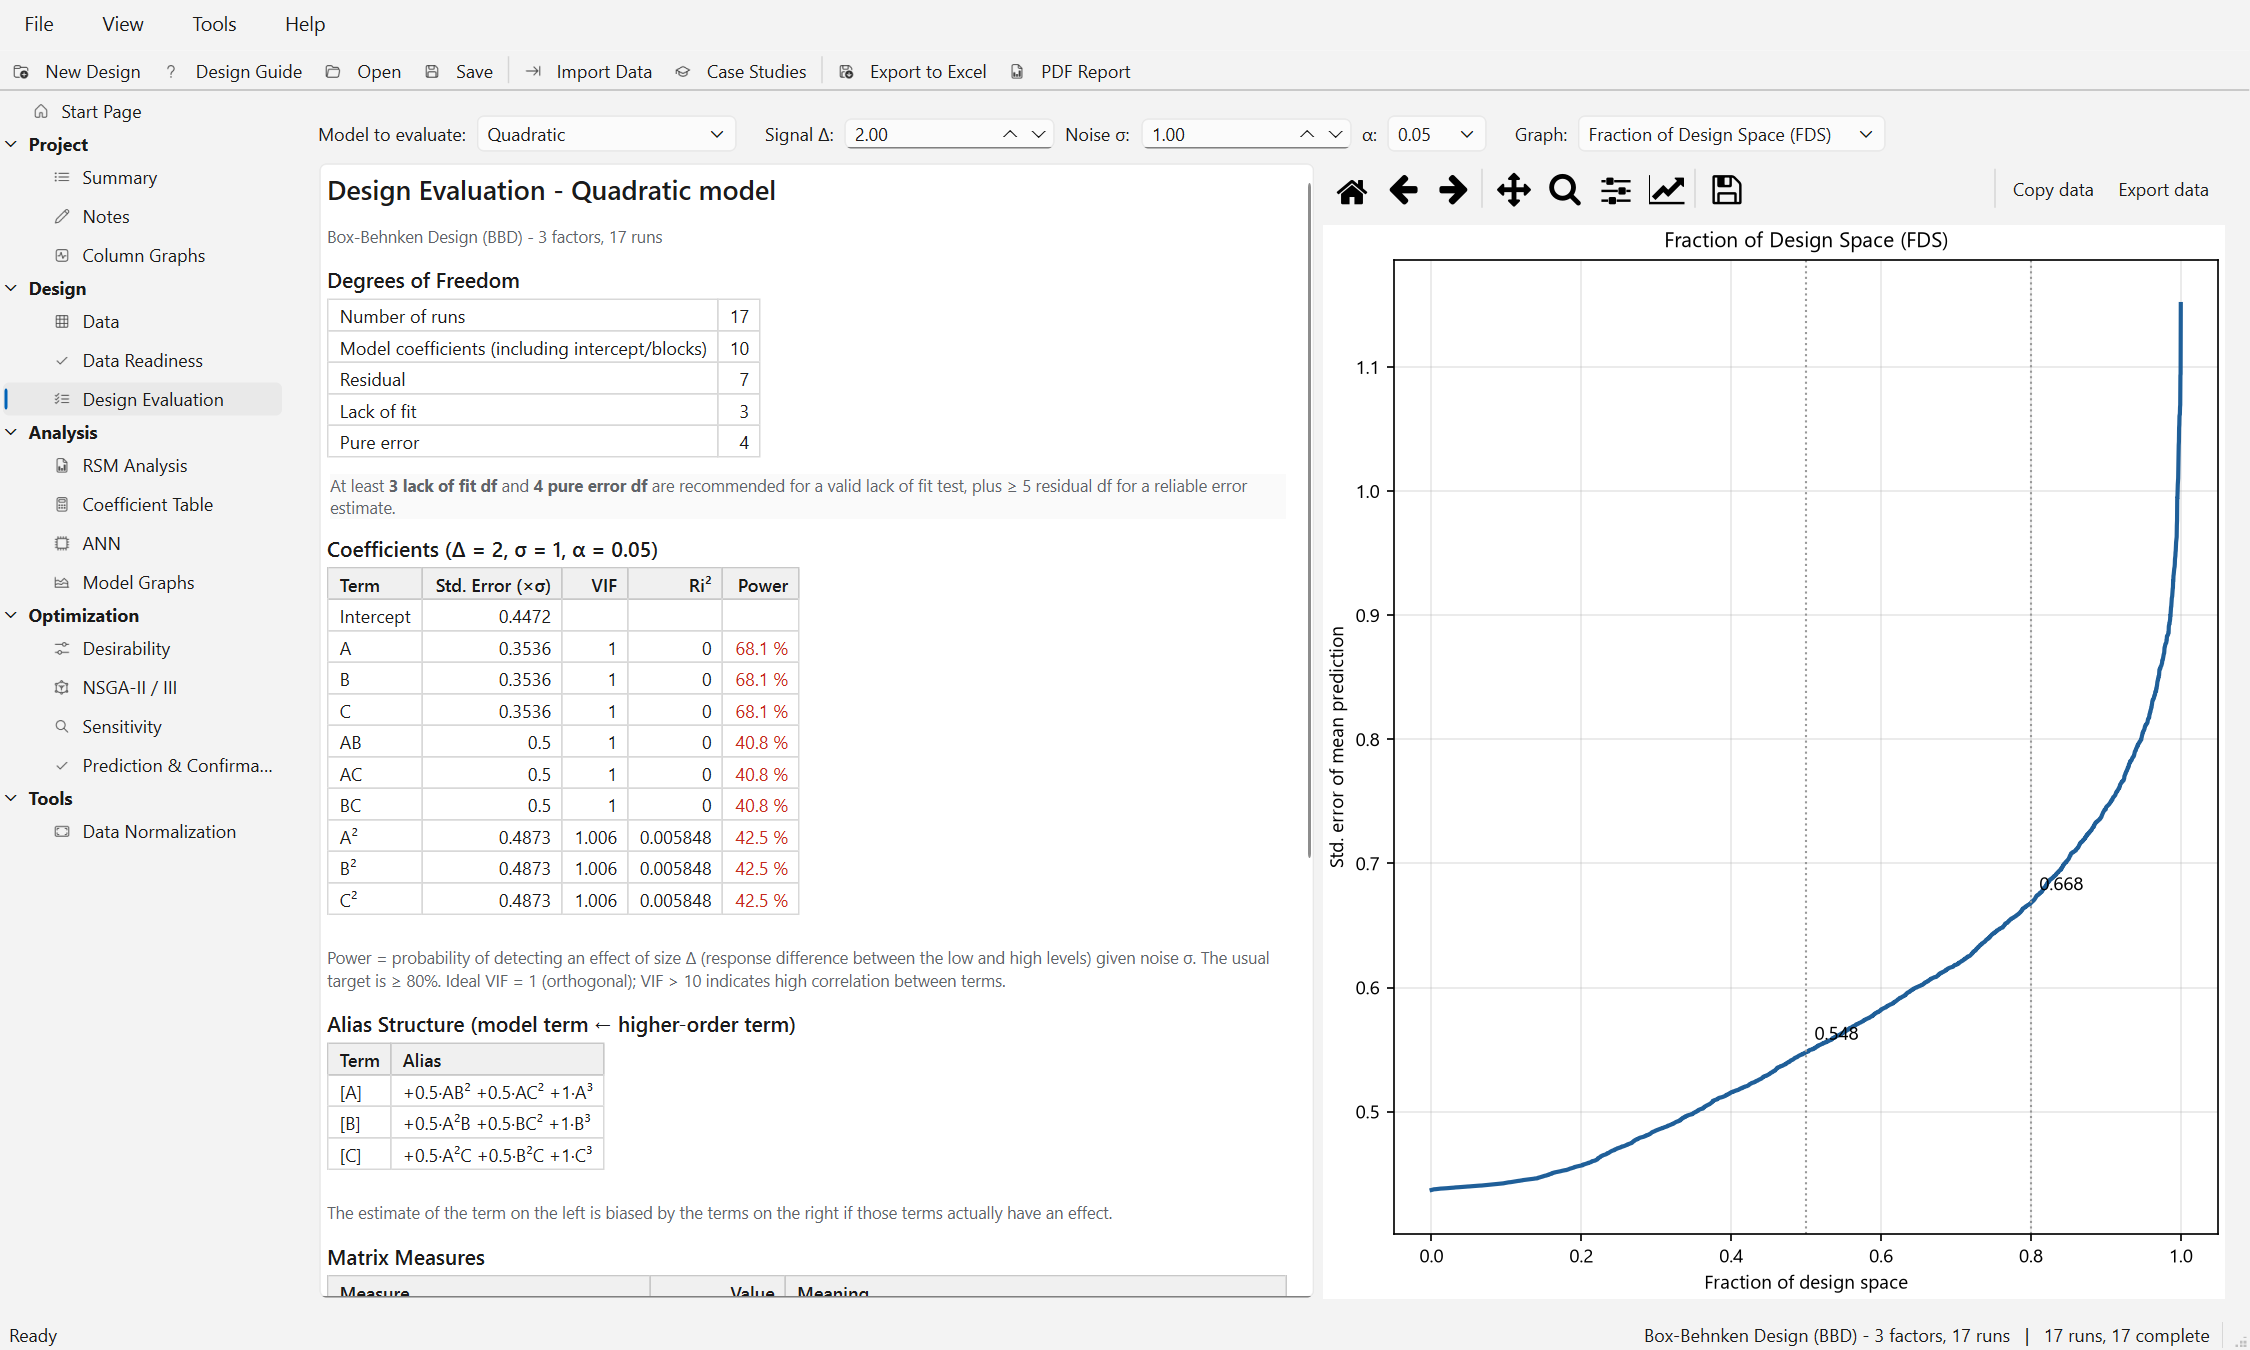
\includegraphics[width=\linewidth]{design_evaluation.png}
\caption{Design Evaluation of the BBD extraction case, quadratic model, $\Delta$ = 2, $\sigma$ = 1, $\alpha$ =
0.05: degrees of freedom, coefficients with standard error, VIF and power (red below 80 \%), alias structure, and the
FDS curve with the standard error at 50 \% (0.548) and 80 \% (0.668) of the region.}
\label{fig:ch04-eval}
\end{figure}

\paragraph{Comparing designs for three factors.} Table~\ref{tab:ch04-compare} compares five designs for the
quadratic model in three factors, computed on this page (seed 12345 for the optimal designs). The rotatable CCD has
the highest power and the lowest prediction variance, at the price of five levels and axial points outside the
range; the face-centered CCD estimates the squared terms poorly (power 32\,\%); the BBD saves three runs but has the
weakest interactions. The optimal designs estimate main effects and interactions very well but the squared terms
poorly, because with only $p = 10$ model points most points go to the boundary; their lack-of-fit and replicate
points are chosen for model checking, not for precision.

\begin{table}[htbp]
\centering
\caption{Design Evaluation of five three-factor designs, quadratic model, $\Delta = 2$, $\sigma = 1$, $\alpha =
0.05$.}
\label{tab:ch04-compare}
\footnotesize
\setlength{\tabcolsep}{4pt}
\begin{tabular}{@{}lccccc@{}}
\toprule
& CCD rotatable & CCD face & BBD & I-optimal & D-optimal \\
\midrule
Runs (residual / pure-error df) & 20 (10 / 5) & 20 (10 / 5) & 17 (7 / 4) & 20 (10 / 5) & 20 (10 / 5) \\
Power main effects (\%) & 91.4 & 81.3 & 68.1 & 94.0--95.2 & 93.7--93.9 \\
Power interactions (\%) & 72.2 & 72.2 & 40.8 & 90.3--92.9 & 87.3--90.2 \\
Power squared terms (\%) & 92.7 & 32.3 & 42.5 & 28.1--34.3 & 22.6--32.7 \\
Condition number & 12.9 & 20.3 & 11.5 & 58.7 & 53.1 \\
D-efficiency (\%) & 61.6 & 36.7 & 34.0 & 45.9 & 44.3 \\
A-efficiency (\%) & 51.6 & 26.5 & 28.9 & 22.3 & 20.9 \\
G-efficiency (\%) & 74.7 & 63.0 & 43.2 & 75.3 & 58.1 \\
I (average prediction variance) & 0.213 & 0.294 & 0.340 & 0.457 & 0.448 \\
$n \cdot I$ & 4.26 & 5.89 & 5.78 & 9.14 & 8.96 \\
FDS SE at 50\,\% / 80\,\% & 0.438 / 0.504 & 0.531 / 0.647 & 0.548 / 0.668 & 0.680 / 0.728 & 0.663 / 0.719 \\
\bottomrule
\end{tabular}
\end{table}

\paragraph{A mixture design.} For the edible film case (14 runs, quadratic Scheff\'e model) the page reports 8
residual df, 4 pure-error df and 4 lack-of-fit df, which satisfies the recommendation. The D-efficiency of 3.2\,\%
is not a sign of a bad design: it reflects the 0--1 range of pseudo-components (limitation 1 above).

\section{Summary}
\label{sec:ch04-summary}

\paragraph{Purpose.} The \ui{Summary} page (title ``Project Summary'') gives an overview of the whole project on one
page, for checking and for reports.

\paragraph{Content.} The box at the top shows the design description, the number of runs and how many have complete
factors (and how many are excluded), the blocks, the number of whole plots, the mixture total and, for designs created in the New
Design dialog, the random seed; constraints follow. The table \emph{Factors} lists for each factor the type (Numeric, Component,
Categoric), the low and high limits, the minimum, maximum, mean and standard deviation of the data, the number of
unique levels and the POE $\sigma$ entered in Factor \& Response Info; categorical factors list their levels with
counts. The table \emph{Responses} lists the type (normal, binomial, poisson), the number of values used ($n$, without
excluded runs), minimum, maximum, mean, SD, the ratio max/min (relevant for a transform), the model (``(selected
terms)'' when terms were edited), the transform, R\textsuperscript{2} (McFadden R\textsuperscript{2} for GLM,
conditional R\textsuperscript{2} for split-plot), adjusted and predicted R\textsuperscript{2}, and the model used for
optimization (RSM or ANN with its architecture). A line ``Other project contents'' counts the ANN models, the
desirability solutions and the NSGA Pareto solutions; the notes close the page. The report panel supports
\ui{Export all tables\dots}.

\begin{figure}[htbp]
\centering
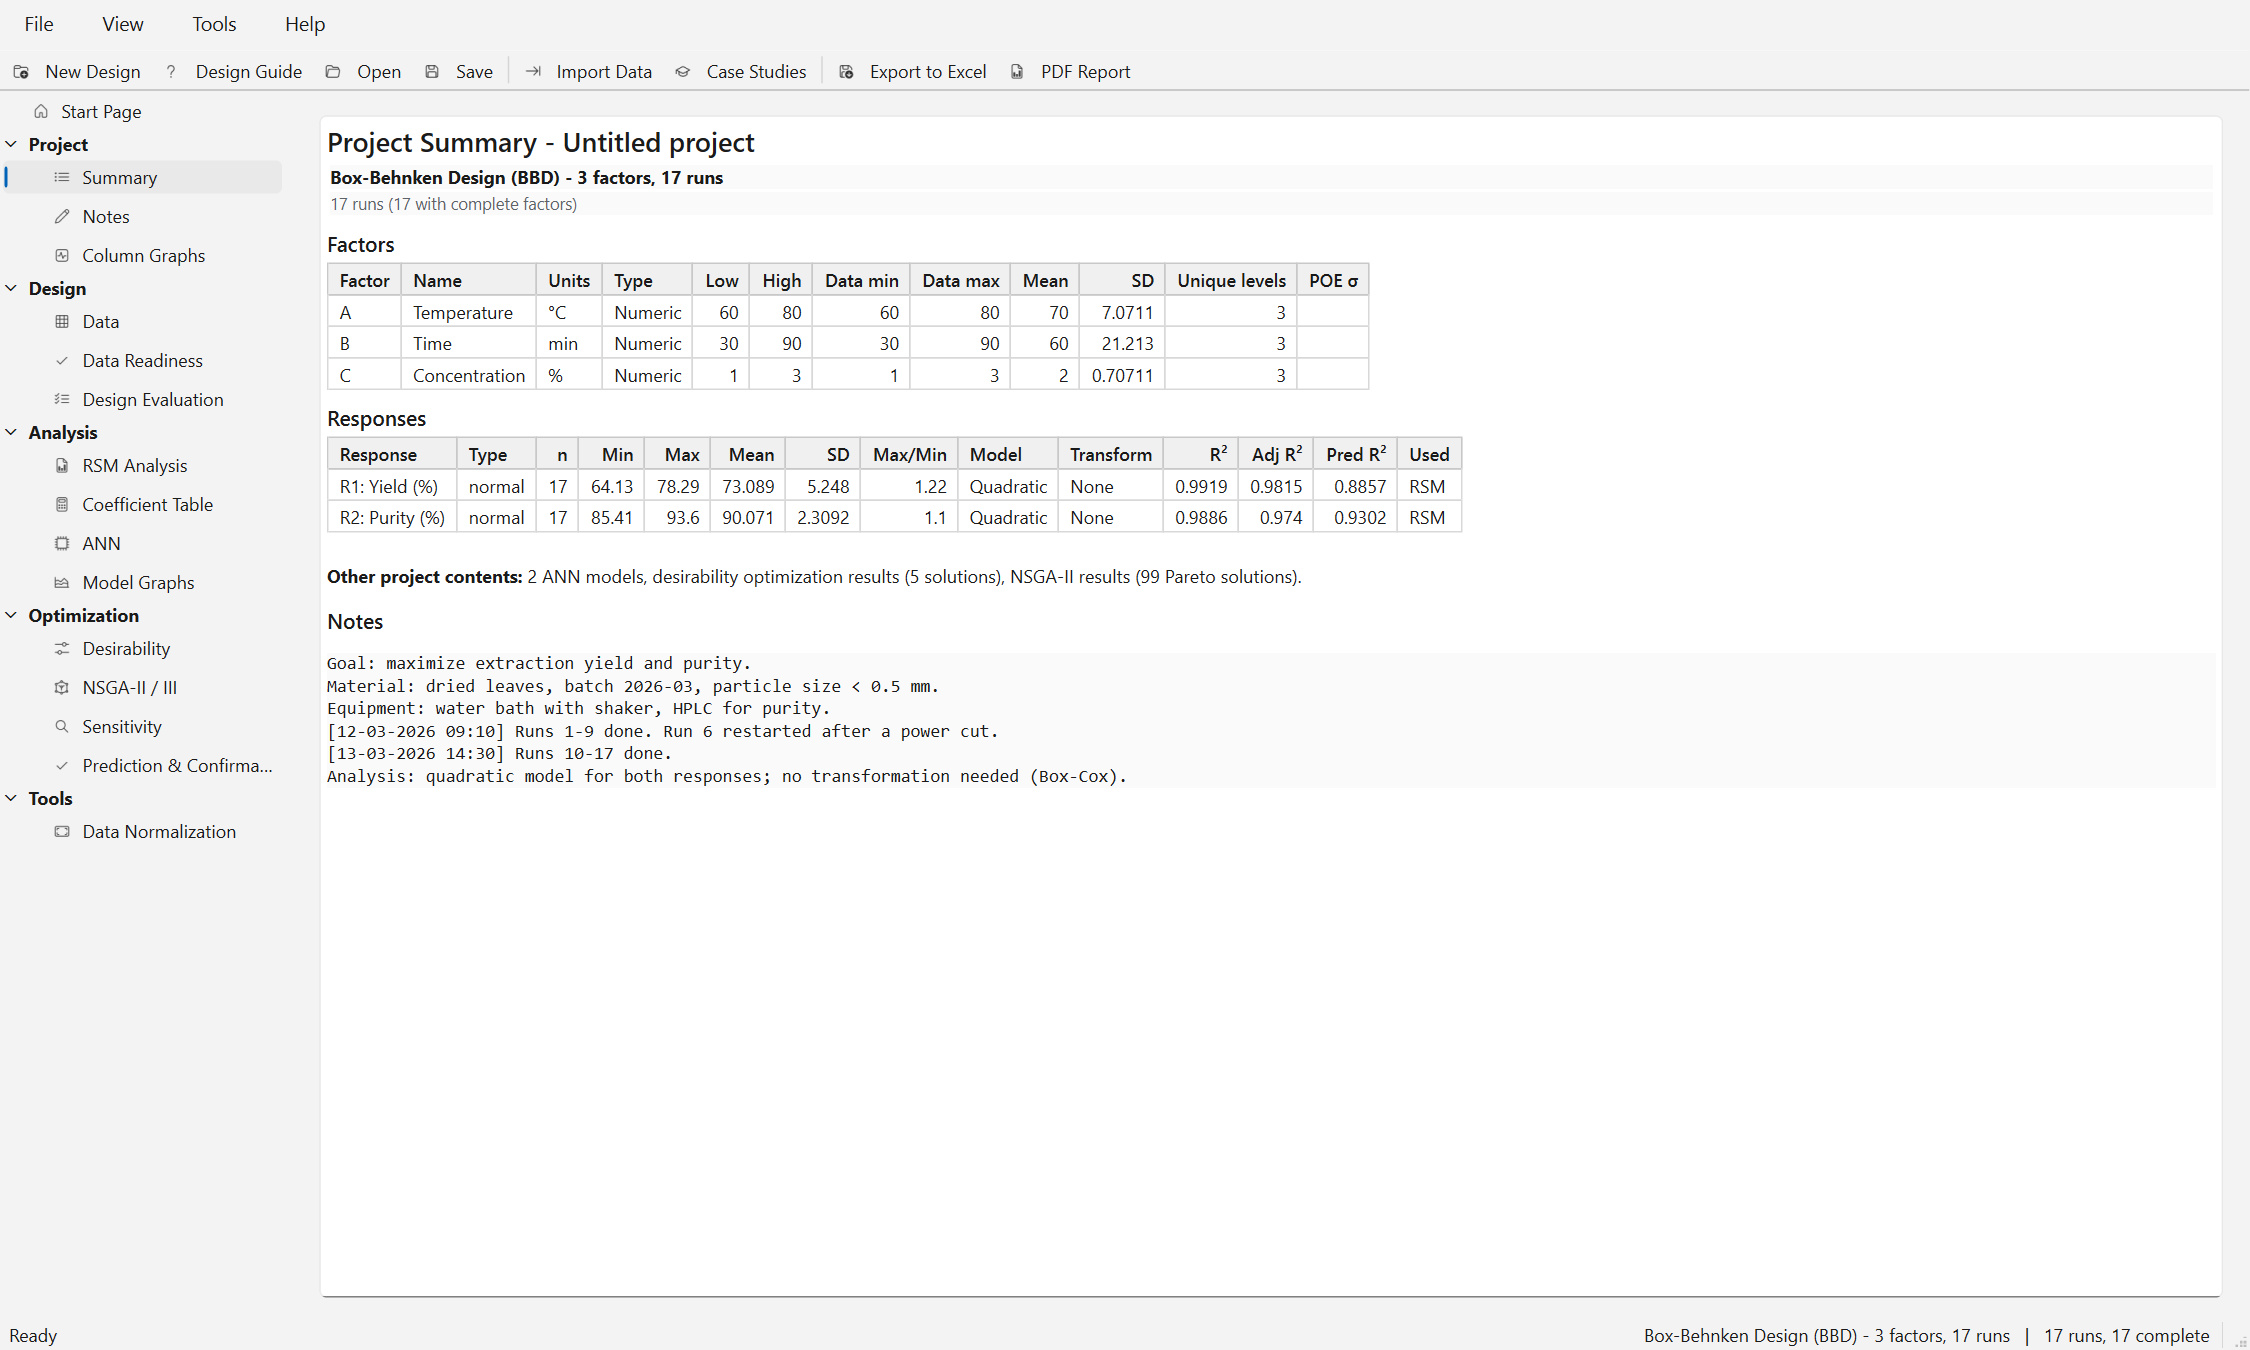
\includegraphics[width=\linewidth]{summary.png}
\caption{Summary of the BBD extraction case after the analysis: factor and response tables (Yield: quadratic,
R\textsuperscript{2} 0.9919, Adj R\textsuperscript{2} 0.9815, Pred R\textsuperscript{2} 0.8857; Purity:
R\textsuperscript{2} 0.9886, Adj 0.974, Pred 0.9302), 2 ANN models, 5 desirability solutions and 99 Pareto
solutions.}
\label{fig:ch04-summary}
\end{figure}

\section{Notes}
\label{sec:ch04-notes}
The \ui{Notes} page is a free text field for the experiment goals, equipment and material conditions, events during
the experiment and analysis decisions. \ui{Insert Date} inserts a time stamp ``[dd-mm-yyyy hh:mm]'' at the cursor.
The notes are saved in the \texttt{.doe} file, shown on the Summary page and printed in the PDF report. Good notes
make an experiment traceable: record deviations from the run order, failed runs and the reasons for excluding any
run.

\begin{figure}[htbp]
\centering
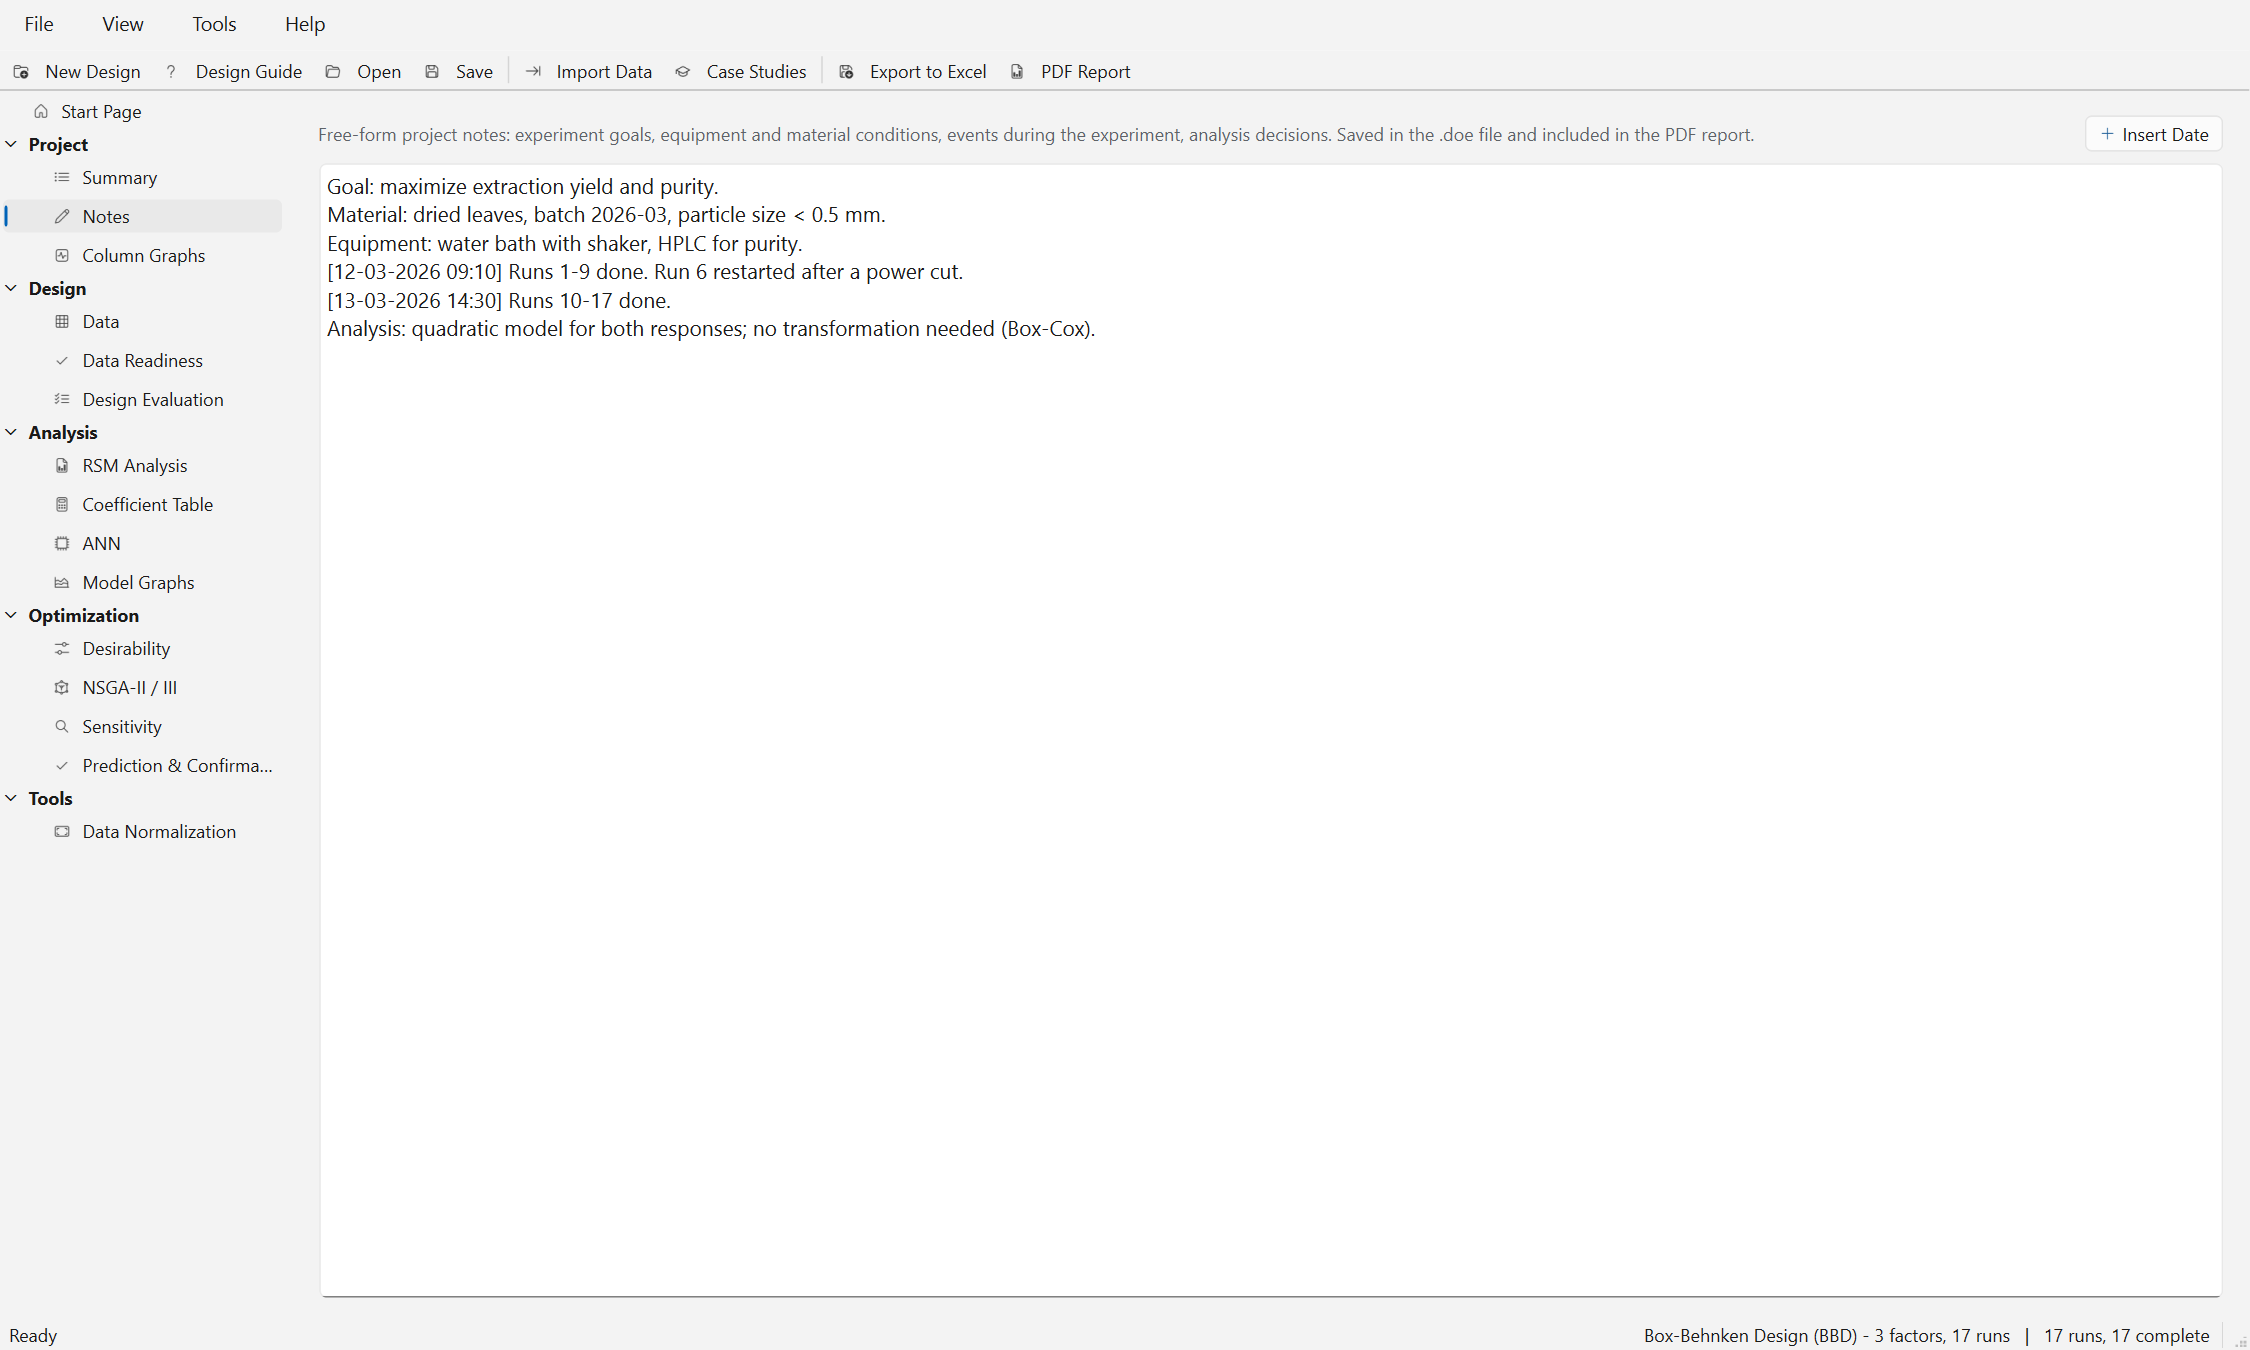
\includegraphics[width=0.85\linewidth]{notes.png}
\caption{Notes page with an example of goals, materials, equipment, dated events and an analysis decision.}
\label{fig:ch04-notes}
\end{figure}

\section{Column Graphs}
\label{sec:ch04-columns}

\paragraph{Purpose.} \ui{Column Graphs} explores the raw data columns before (and besides) modeling: distributions,
relations between factors and responses, trends over the run order and correlations in historical data.

\paragraph{Columns.} ``Std Order'', ``Run'', ``Block'' (if blocked), every factor in actual units (categorical
factors as level index with the level names on the axis), every response (excluded runs empty) and ``Residual R1'',
\dots{} for every least-squares response with a fitted model ($y - \hat y$).

\paragraph{Options.} \ui{Type:} \ui{Scatterplot} (default), \ui{Histogram}, \ui{Box plot}, \ui{Scatter matrix};
\ui{Color by:} (None or any column, default Run); \ui{X axis:} (default the first factor); \ui{Y axis:} (default the
first response); \ui{Z axis (3D):} (None, or a column for a 3-D scatter); \ui{Trend line (linear regression)}.

\paragraph{Output.}
\begin{itemize}
\item \emph{Scatterplot}: Y against X with the label ``Correlation (Pearson r) = \dots{} $\cdot$ Spearman $\rho$ =
\dots{} $\cdot$ n = \dots'' and, optionally, the least-squares line $y = a x + b$. Numeric colouring uses a continuous
color map with a color bar, categorical colouring a legend.
\item \emph{Histogram}: $\min(50, \max(8, \lfloor\sqrt{n}\rfloor))$ bins (a bar chart of counts for categorical
columns), with $n$, mean, SD, median and skewness.
\item \emph{Box plot}: Y grouped by the distinct values of X if X is categorical or has at most 12 distinct values,
otherwise by 5 quantile groups; the Kruskal--Wallis test reports whether the groups differ ($\alpha = 0.05$).
\item \emph{Scatter matrix}: up to the first 8 factor and response columns, histograms on the diagonal and $r$ in
each panel (red when $|r| \ge 0.5$); at most 2000 random complete runs are drawn.
\end{itemize}
The heat map on the right shows the Pearson correlation of all pairs of columns; clicking a cell plots that pair.
Correlations use the pairwise complete rows and need more than two rows. In a designed experiment the factor columns
are nearly uncorrelated; strong correlations between factors in historical data warn that their effects cannot be
separated (check VIF on the Design Evaluation page). A trend of a response or a residual against \ui{Run} indicates
drift. Every plot has \ui{Copy data} and \ui{Export data\dots}.

\begin{figure}[htbp]
\centering
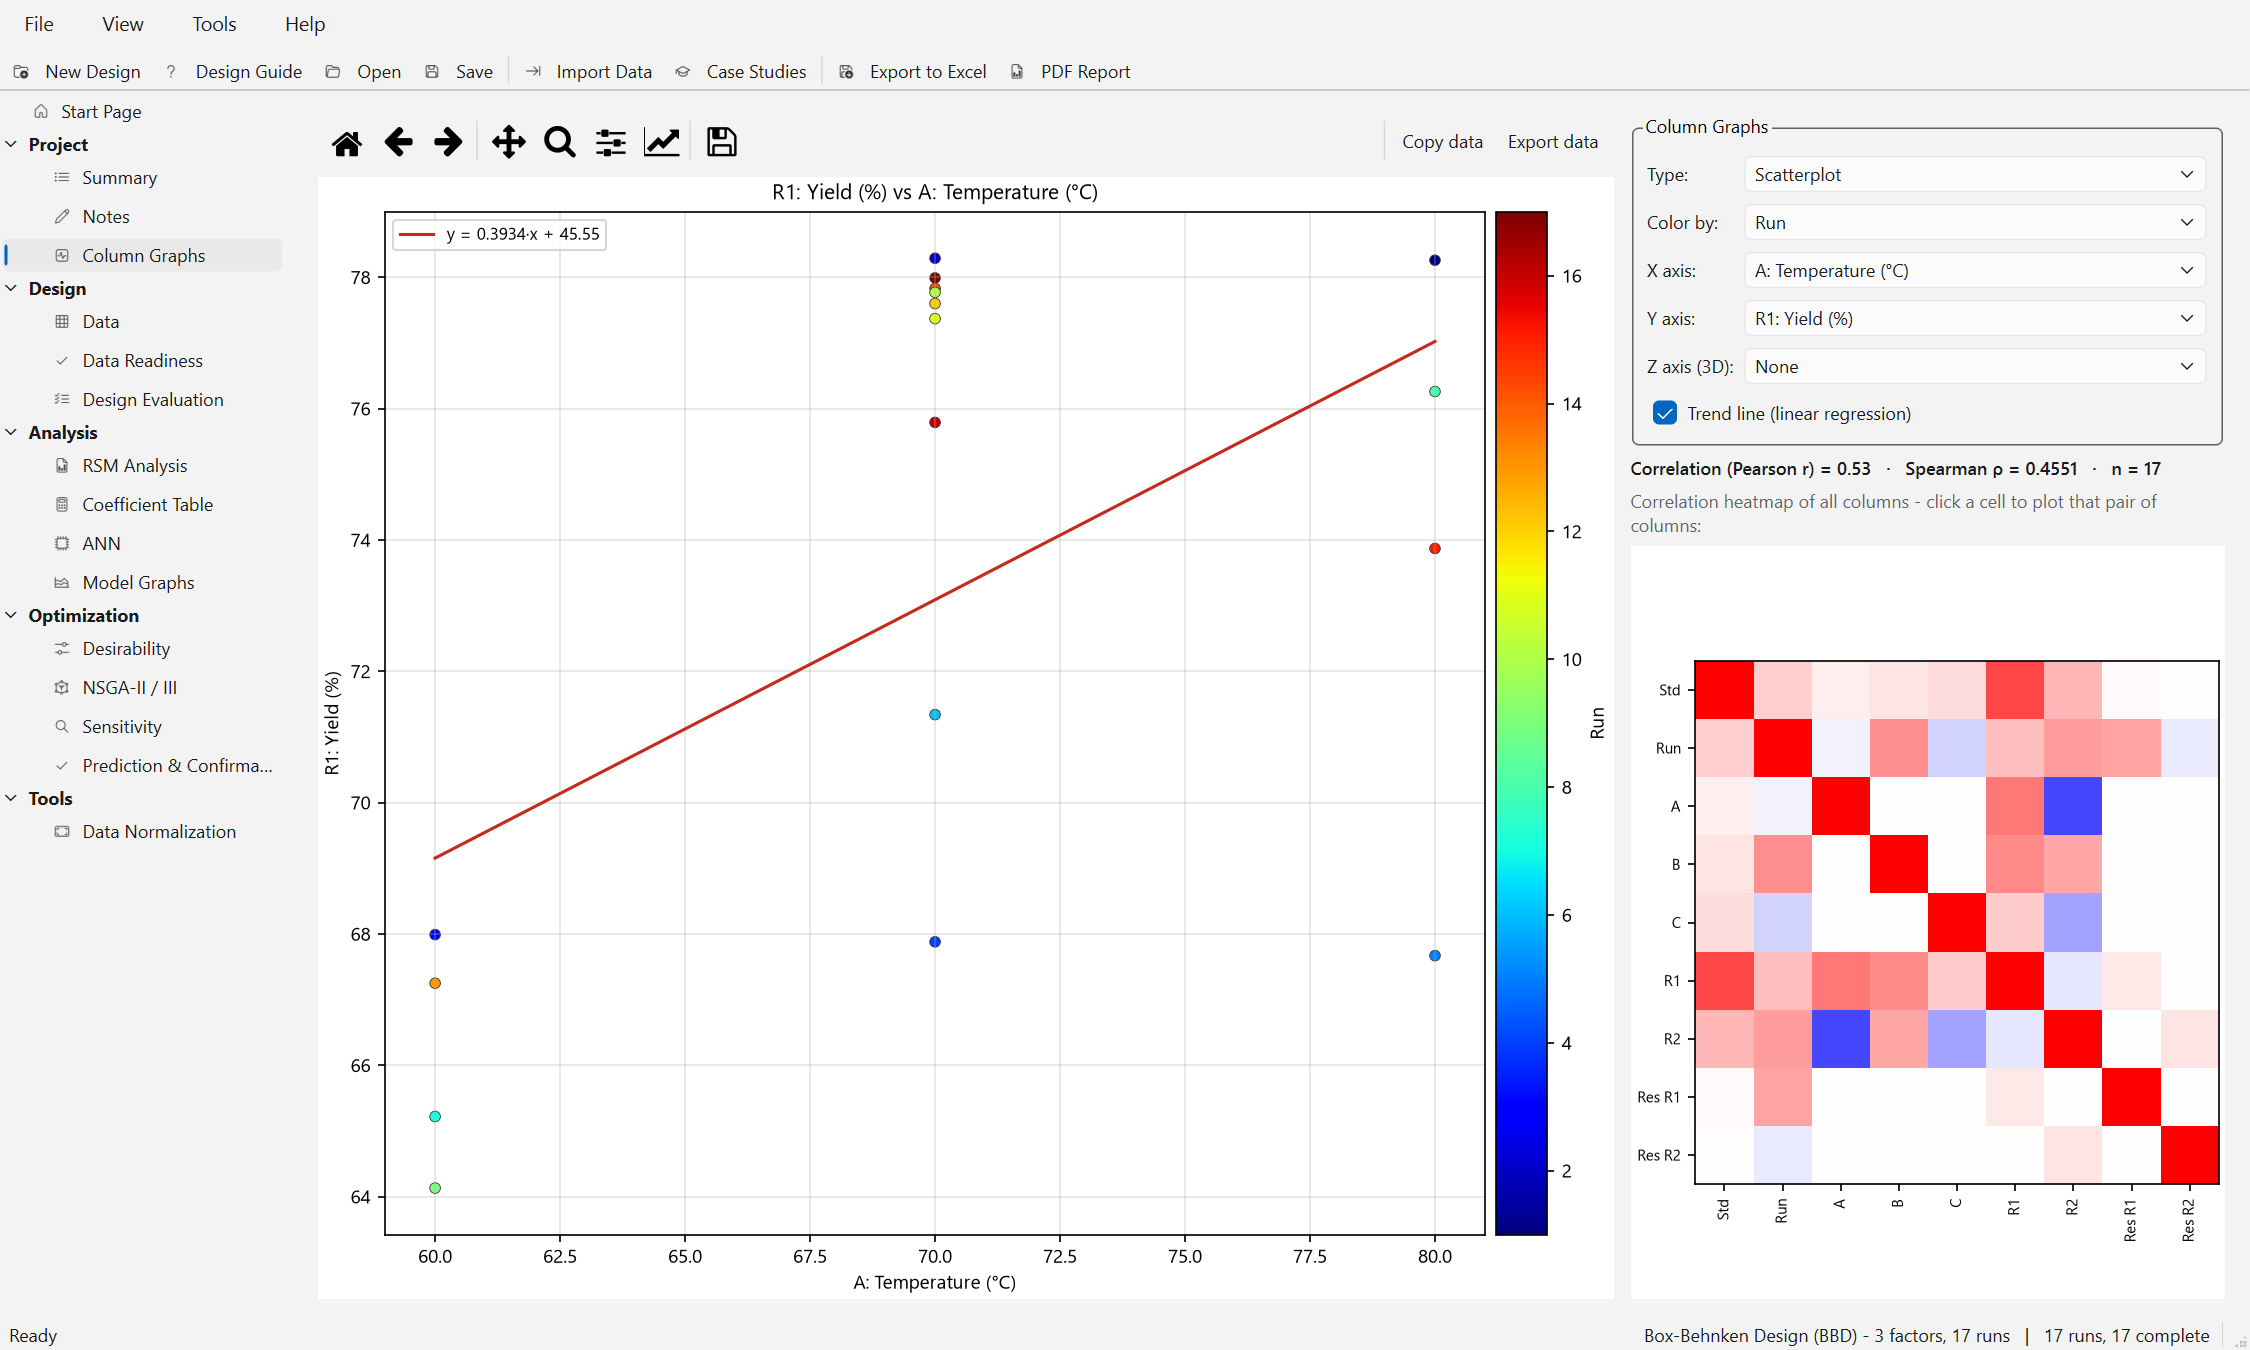
\includegraphics[width=\linewidth]{column_graphs.png}
\caption{Column Graphs for the BBD extraction case: Yield against Temperature, coloured by run, with the trend line
$y = 0.3934x + 45.55$, Pearson r = 0.53 and Spearman $\rho$ = 0.4551 ($n$ = 17); correlation heat map of all
columns.}
\label{fig:ch04-columngraphs}
\end{figure}

\paragraph{Example.} In Figure~\ref{fig:ch04-columngraphs} the linear correlation between Temperature and Yield is
only 0.53 although Temperature is the strongest factor: the effect is curved (a maximum inside the range), which a
correlation coefficient does not capture. This is why factor effects are judged from the model, not from raw
correlations.

\section{Coefficient Table}
\label{sec:ch04-coef}
The \ui{Coefficient Table} (group \ui{Analysis}) shows the coded coefficients of all responses side by side: one row
per model term, one column per response with a computable RSM model. A cell holds the coefficient (coded units or
pseudo-components) and, with \ui{Show p-values} on, its $p$-value; the background is dark green for $p < 0.01$, light
green for $p < 0.05$ and yellow for $p < 0.1$. An empty cell means that the term is not in that response's model.
The footer rows give the transform, the model, the model $p$-value, R\textsuperscript{2}, adjusted and predicted
R\textsuperscript{2} and the model used for optimization. Because the coefficients are in coded units, their sizes can
be compared across factors and responses: a factor with a large positive coefficient for one response and a large
negative one for another signals a trade-off that the optimization must resolve. For responses that use an ANN, the
table still shows the RSM coefficients. The $p$-values come from the same tests as in the RSM analysis; the theory is
given in Chapter~\ref{chap:5}. The report supports \ui{Export all tables\dots}.

\begin{figure}[htbp]
\centering
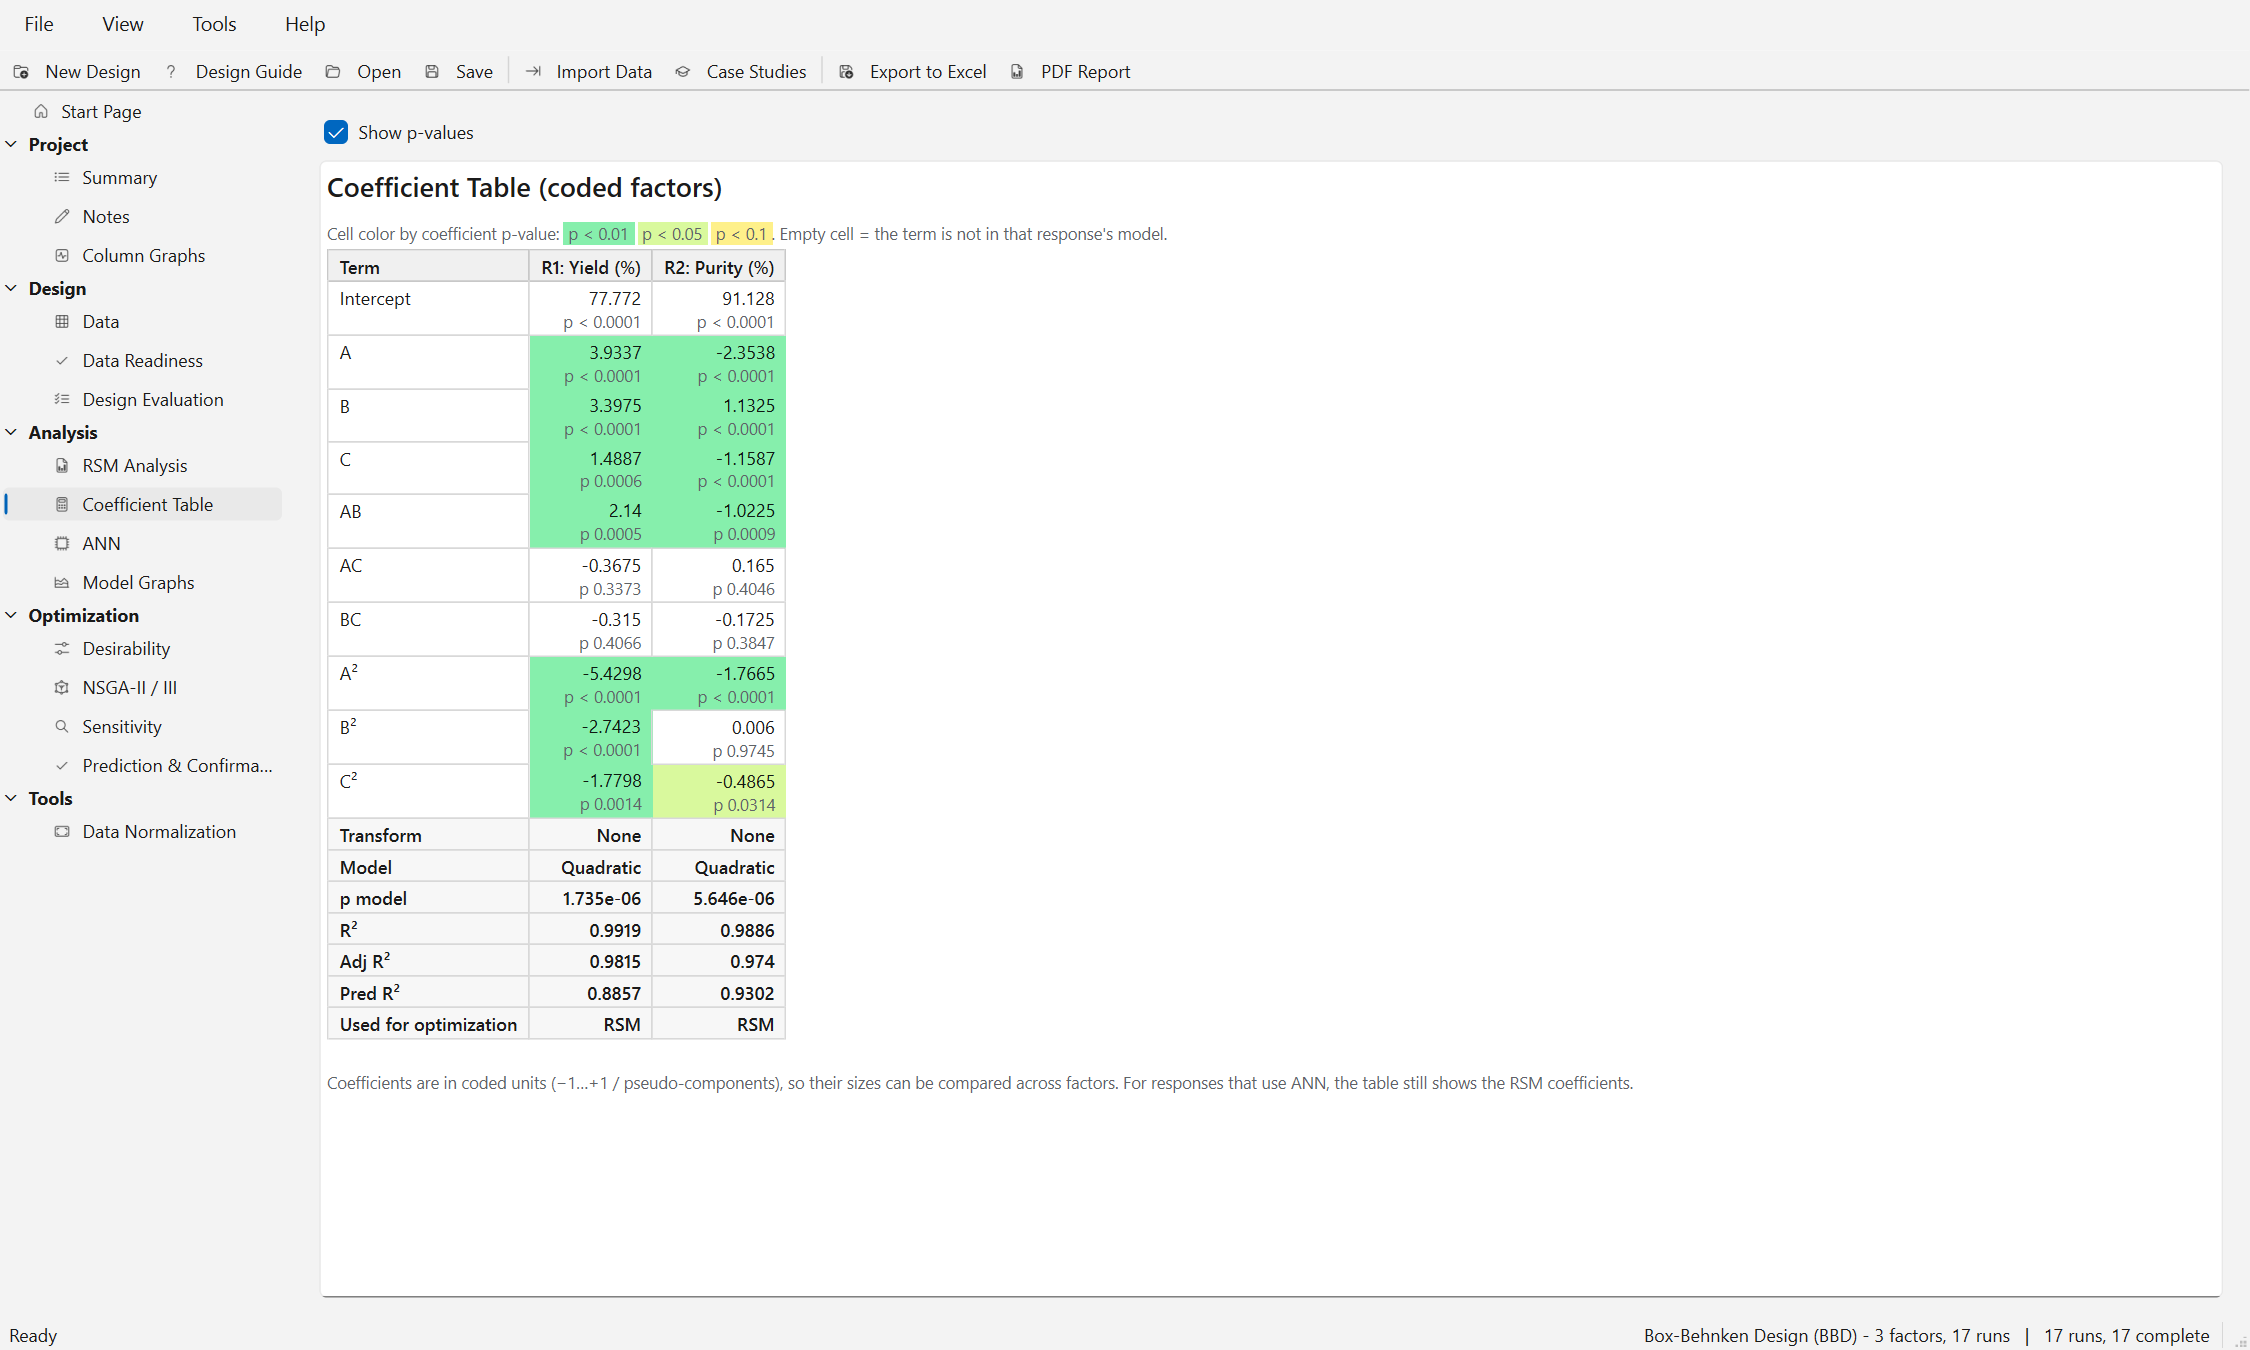
\includegraphics[width=\linewidth]{coefficient_table.png}
\caption{Coefficient Table of the BBD extraction case: Yield intercept 77.772, A 3.9337, A\textsuperscript{2}
$-5.4298$; Purity A $-2.3538$. AC and BC are not significant for either response.}
\label{fig:ch04-coef}
\end{figure}

\section{Data Normalization}
\label{sec:ch04-normalization}

\paragraph{Purpose.} Variables with different units and ranges (pH 2--10 and a concentration of 20--200 mg/L) are
put on a common scale so that no variable dominates only because its numbers are large. RSM uses coded factors
automatically, and the ANN normalizes its inputs and outputs with the method chosen on the ANN page; this page
(\menupath{Tools $\rightarrow$ Data Normalization}) is for viewing, comparing and exporting normalized data. It does
not change the project.

\paragraph{Options.} \ui{Method:} ``Min-max to [-1, 1] (mapminmax) - recommended'' (default), ``Min-max to [0,
1]'', ``Z-score standardization (mapstd): mean 0, SD 1'' and ``No normalization (for comparison)''; check boxes
\ui{Factors} and \ui{Responses} (both on); button \ui{Export to Excel\dots}.

\paragraph{Theory.} Every column is transformed as
\begin{equation}
x' = b + \frac{x - o}{s},
\label{eq:ch04-norm}
\end{equation}
with offset $o$, scale $s$ and base $b$:
\begin{center}
\small
\begin{tabular}{@{}lcccc@{}}
\toprule
Method & $o$ & $s$ & $b$ & Range of $x'$ \\
\midrule
mapminmax & $\min x$ & $(\max x - \min x)/2$ & $-1$ & $[-1, 1]$ \\
min-max [0, 1] & $\min x$ & $\max x - \min x$ & 0 & $[0, 1]$ \\
z-score (mapstd) & mean & SD ($n-1$) & 0 & mean 0, SD 1 \\
none & 0 & 1 & 0 & original \\
\bottomrule
\end{tabular}
\end{center}
A zero scale (a constant column) is replaced by 1; missing values are ignored. Categorical factors use the level
index. The data are all runs in run order, without the excluded runs (a note states how many are left out). The
minimum and maximum come from the data, not from the design limits, so a new value outside the observed range maps
outside $[-1, 1]$.

\paragraph{Output.} The tab \ui{Normalized Data} lists Run and the normalized columns (5 decimals); the tab
\ui{Statistics \& Parameters} lists for each variable the minimum, maximum, mean, SD, range, offset, scale, base and
the new minimum and maximum. The figure shows box plots before (original units) and after normalization (a random
sample of 5000 rows for very large data; factors and responses in different colors). \ui{Export to Excel\dots}
writes the sheets ``Normalized'' (method and formula in the first row), ``Original Data'' and ``Parameters'' (offset,
scale and base per variable, so the transformation can be reproduced). The tables support \ui{Export table\dots}
and the plot \ui{Copy data} and \ui{Export data\dots}.

\paragraph{Example.} In the dye adsorption case pH ranges from 2.13 to 9.97, so mapminmax uses $o = 2.13$ and
$s = 3.92$; Initial Concentration ranges from 22.1 to 198.6 ($s = 88.25$) and Removal Efficiency from 2.73 to 58.45
($s = 27.86$). The first run in run order (pH 4.93, dose 3.29 g/L, time 81.7 min, concentration 147 mg/L, removal
35.57 \%) becomes $(-0.286, 0.606, 0.305, 0.415, 0.179)$. Figure~\ref{fig:ch04-norm} shows how the very different
scales before normalization collapse into the common range.

\begin{figure}[htbp]
\centering
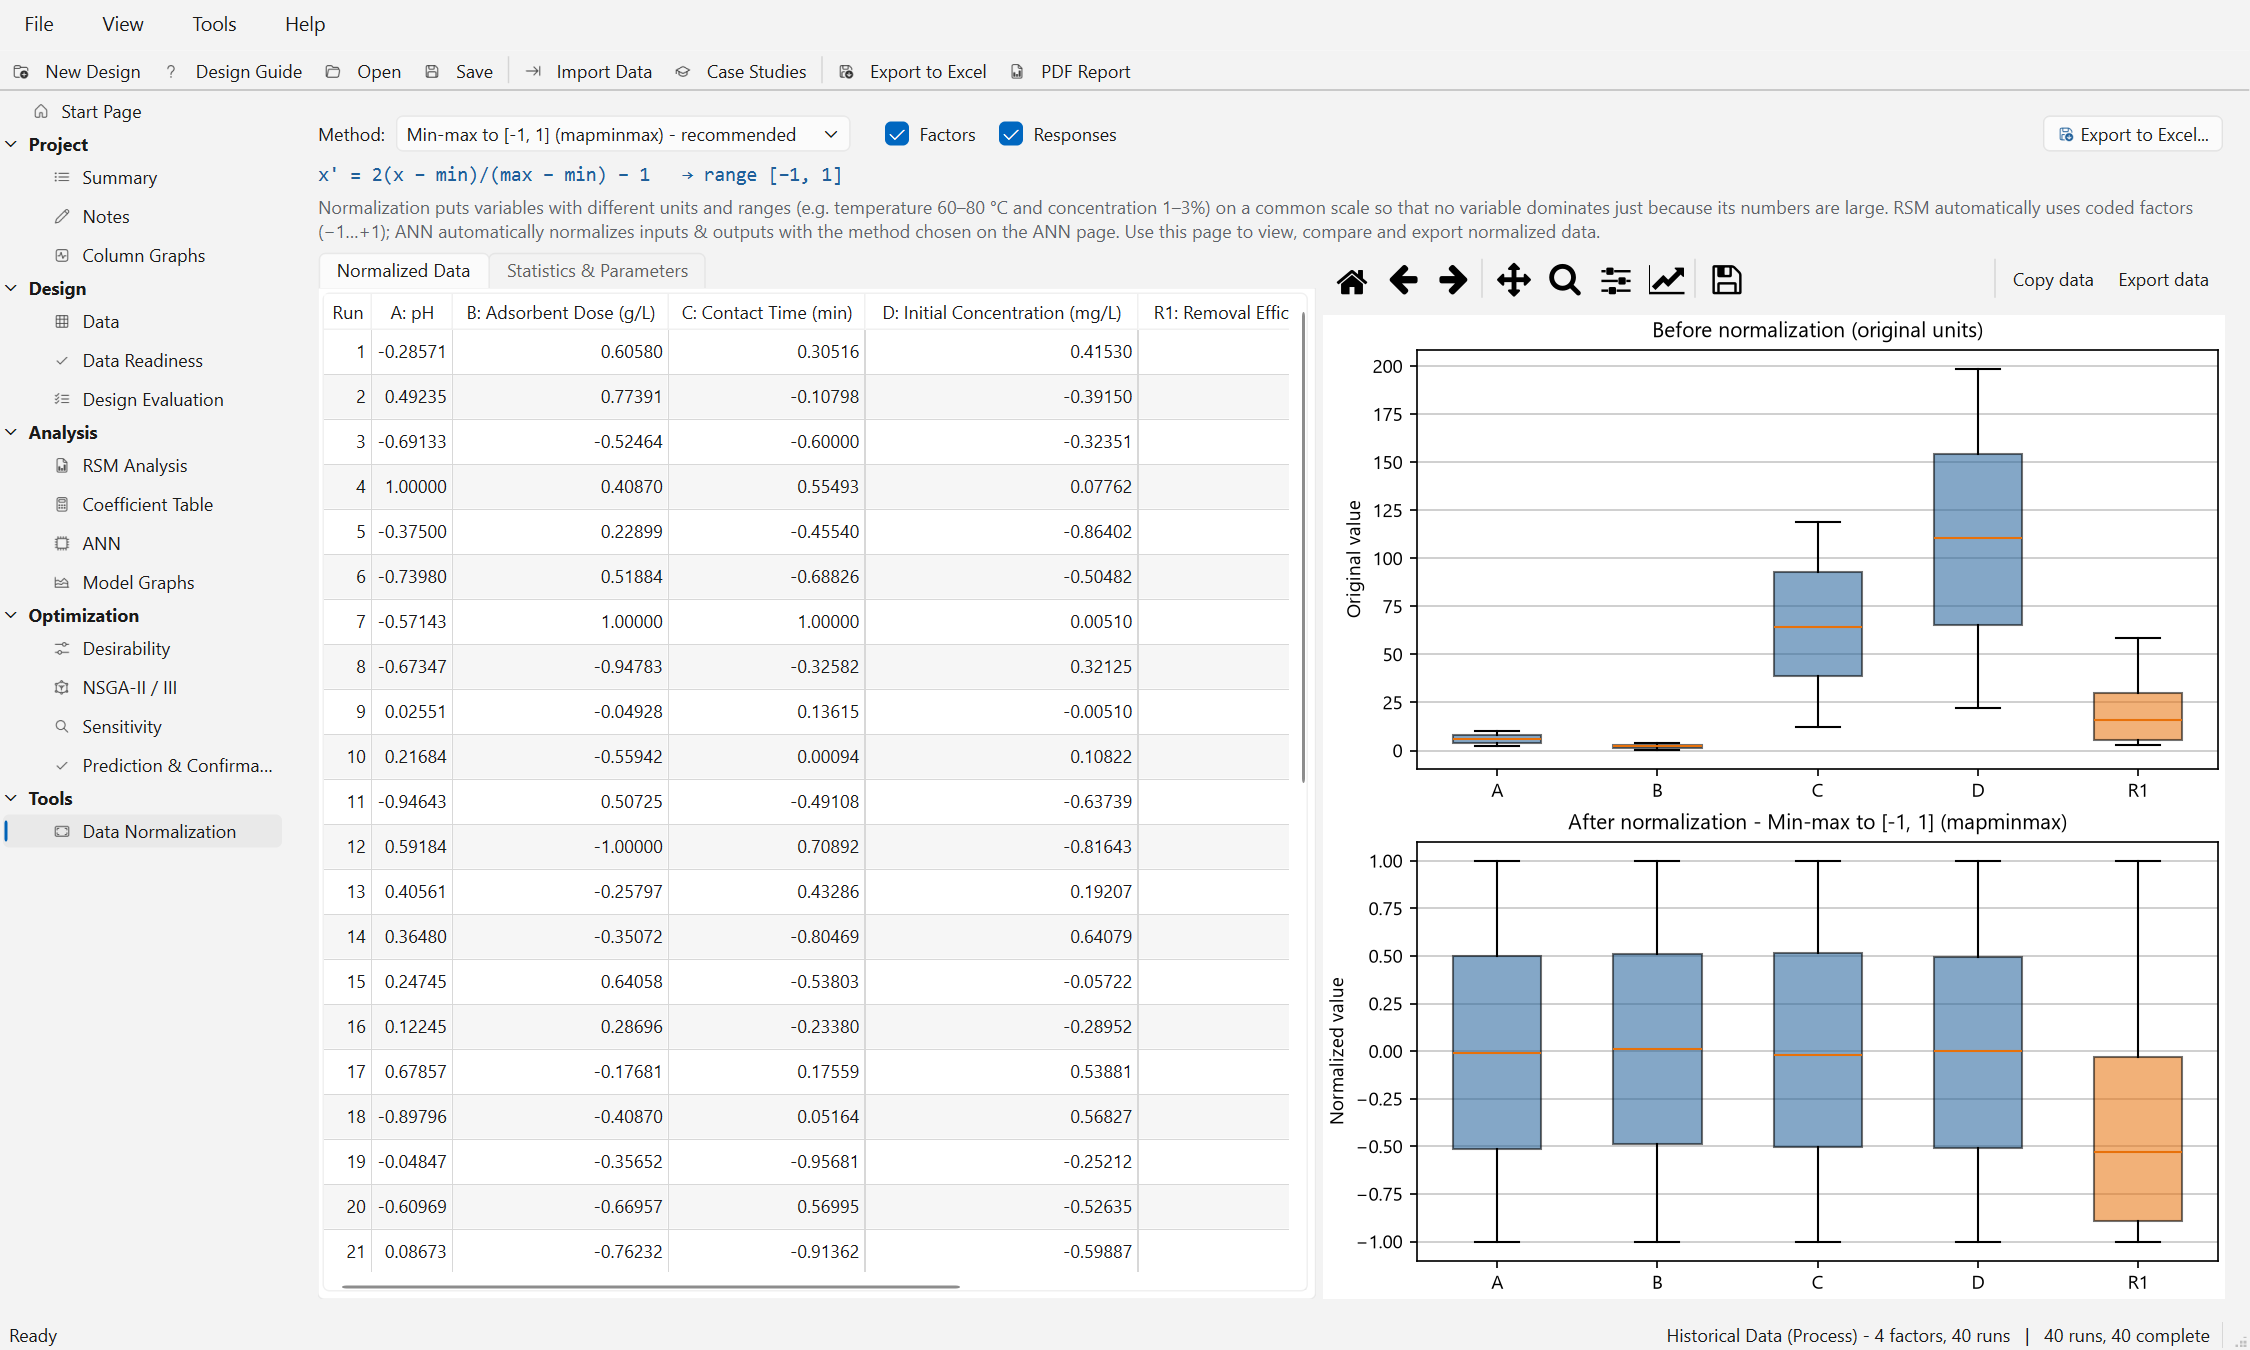
\includegraphics[width=\linewidth]{normalization.png}
\caption{Data Normalization of the dye adsorption case with mapminmax: formula, normalized data and box plots
before and after normalization.}
\label{fig:ch04-norm}
\end{figure}

% Chapter 5: Response Surface Analysis (RSM Analysis page and Coefficient Table page)
\chapter{Response Surface Analysis}\label{sec:ch05-rsm}\label{chap:5}

The \ui{RSM Analysis} page (navigation group \ui{Analysis}) is where a regression model is chosen,
fitted and checked for each response. Everything that the later pages use (model graphs, desirability,
NSGA-II, sensitivity, prediction) is built on the model that is selected here, unless the response is
switched to an ANN model on the \ui{ANN} page. This chapter describes the page from top to bottom: the
toolbars, the term list and the six sub-tabs \ui{Fit Summary}, \ui{ANOVA}, \ui{Model Equation},
\ui{Diagnostics}, \ui{Box-Cox} and \ui{Effects (Factorial)}. It also covers the two special analyses that
replace ordinary least squares for some responses (logistic and Poisson regression, and the split-plot
REML analysis) and the \ui{Coefficient Table} page, which shows the coefficients of all responses side by
side.

The numbers in the examples come from the built-in case studies (\menupath{File $\rightarrow$ Case
Studies}). The case studies use fixed data, so you can reproduce every value.

\section{The RSM Analysis page at a glance}\label{sec:ch05-page}

\subsection*{Purpose}
The page answers three questions for one response at a time: which polynomial model describes the data
adequately, which terms of that model are needed, and whether the assumptions behind the statistical tests
are met.

\subsection*{How to use (typical workflow)}
\begin{enumerate}
  \item Select the response in \ui{Response:}.
  \item Read the \ui{Fit Summary} sub-tab and click \ui{Use Suggested Model} (or choose an order in
        \ui{Model:} yourself).
  \item Read the \ui{ANOVA} sub-tab: model significance, term p-values, lack of fit and the fit
        statistics.
  \item Remove terms that are not needed, either by unchecking them in the term list or with
        \ui{Backward Elimination}.
  \item Check the residuals on the \ui{Diagnostics} sub-tab and, if needed, the \ui{Box-Cox} sub-tab.
        Apply a transformation or exclude a faulty run, then go back to step 2.
  \item Read the final equation on the \ui{Model Equation} sub-tab.
  \item Repeat for the other responses and compare them on the \ui{Coefficient Table} page.
\end{enumerate}
Every change (order, terms, transformation, excluded runs) is stored in the project and immediately used
by the \ui{Coefficient Table}, \ui{Model Graphs}, optimization and prediction pages.

\begin{figure}[htbp]\centering
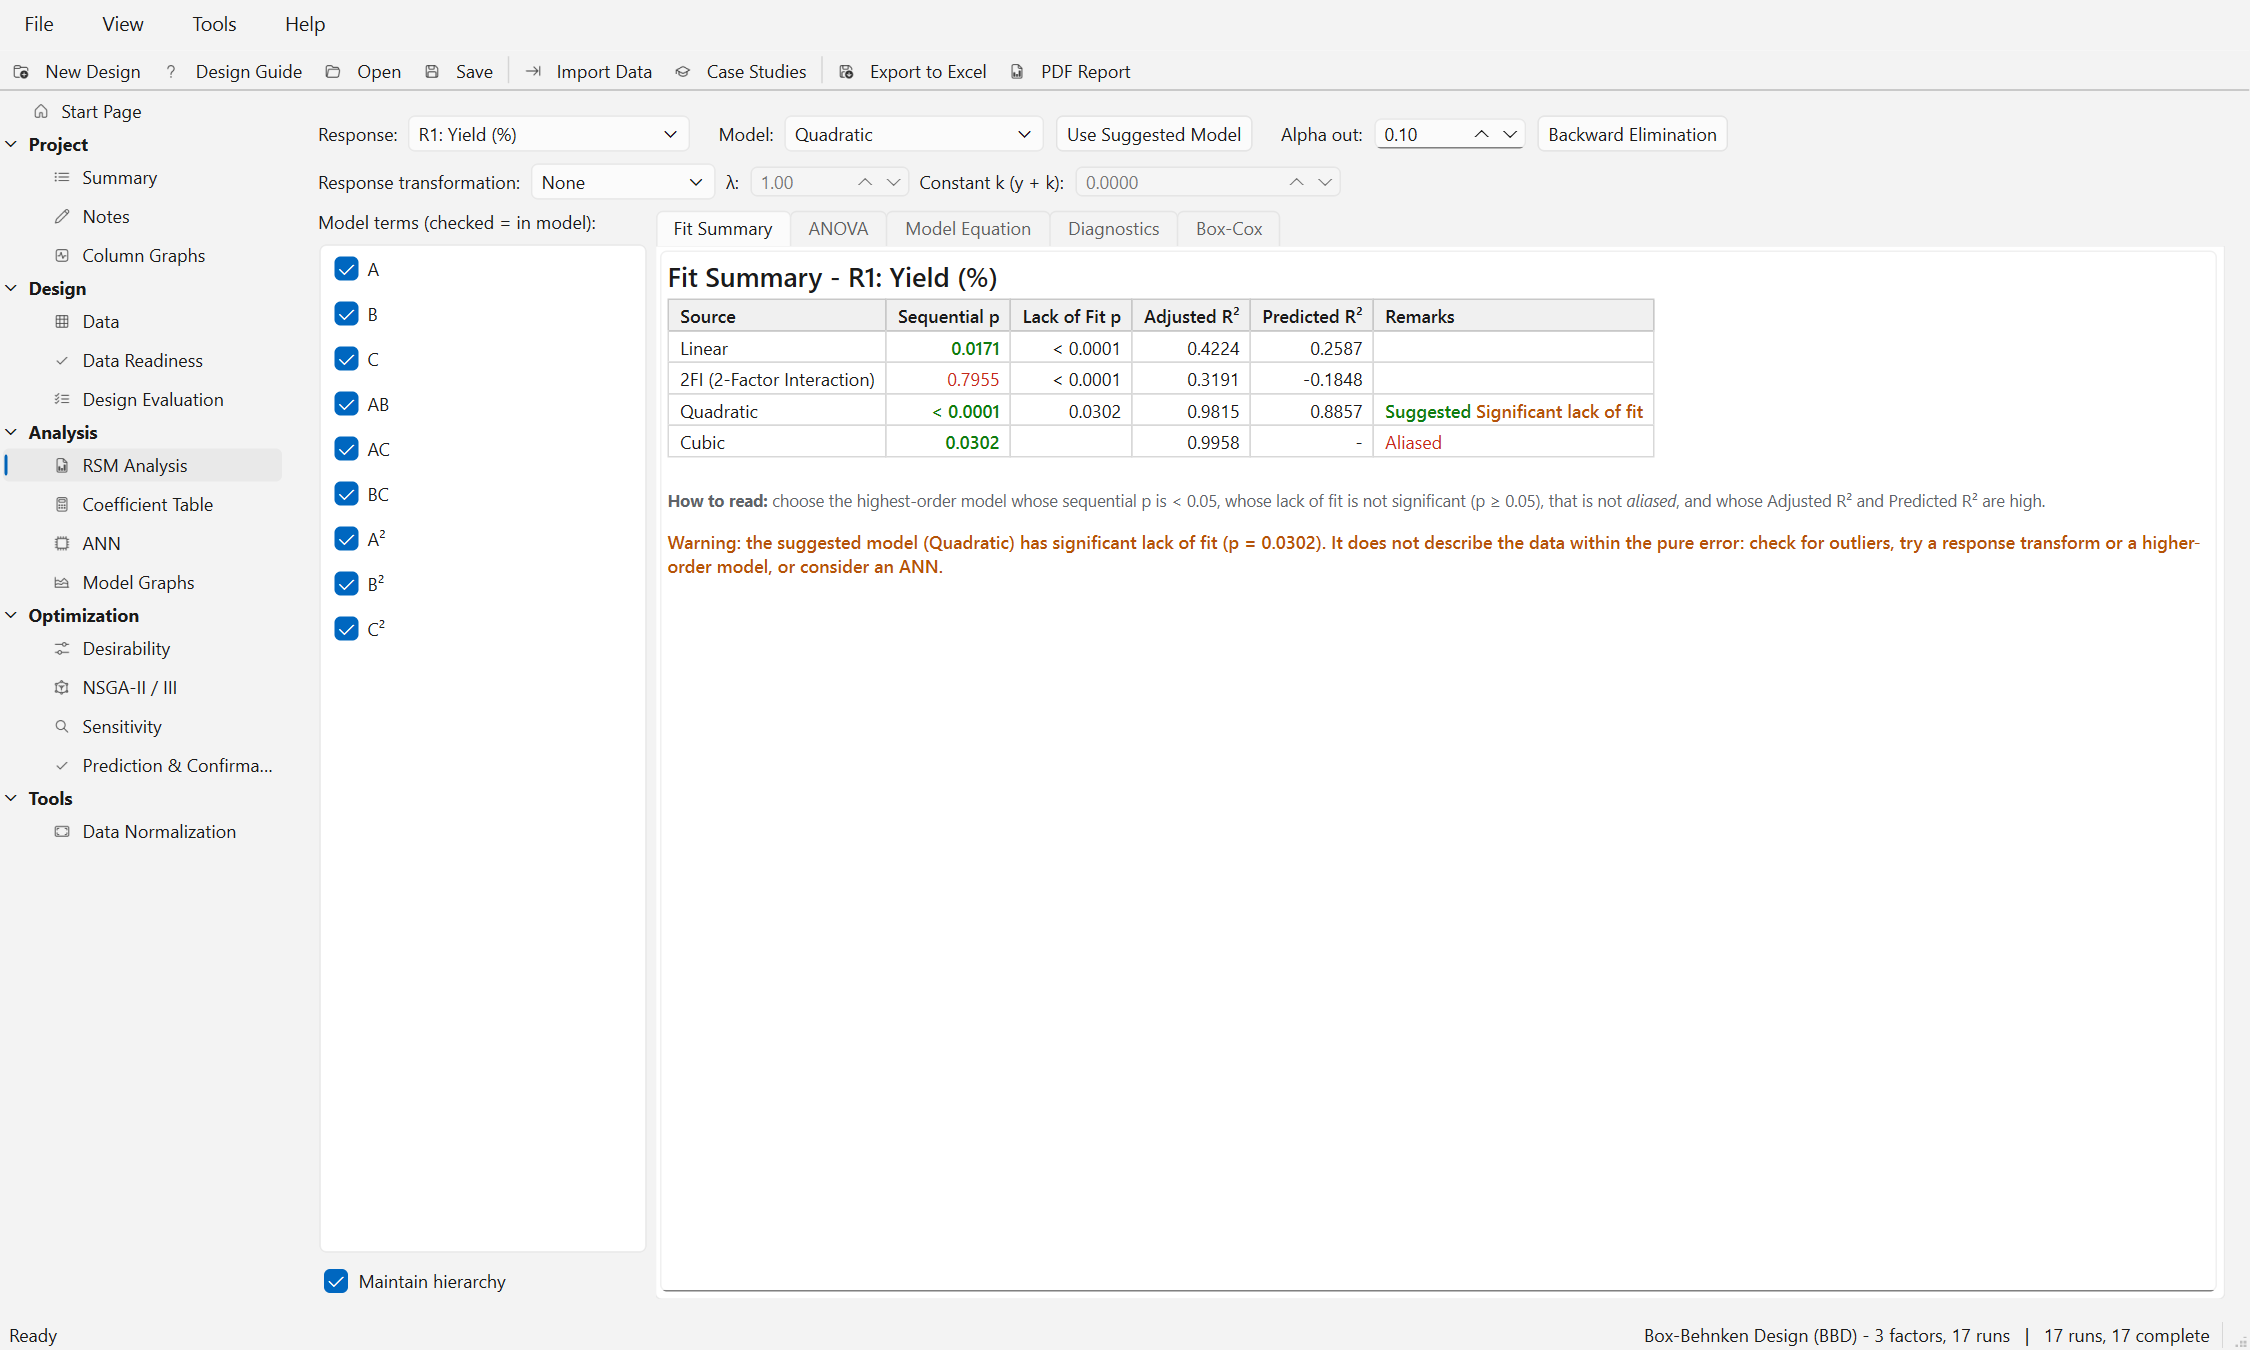
\includegraphics[width=\linewidth]{rsm_fit_summary.png}
\caption{RSM Analysis page, \ui{Fit Summary} sub-tab, for the response Yield of the Box-Behnken extraction
case. Top: the two toolbar rows. Left: the term list with \ui{Maintain hierarchy}. Right: the sequential
model table with the suggested model (Quadratic, remark \ui{Significant lack of fit}) and, below the note, the
lack-of-fit warning (p = 0.0302).}
\label{fig:ch05-fitsummary}
\end{figure}

\subsection*{Toolbar controls}
Table~\ref{tab:ch05-toolbar} lists the controls of the two toolbar rows above the sub-tabs
(Figure~\ref{fig:ch05-fitsummary}).

\begin{table}[htbp]\centering\small
\caption{Toolbar controls of the RSM Analysis page.}\label{tab:ch05-toolbar}
\begin{tabularx}{\linewidth}{@{}>{\raggedright\arraybackslash}p{3.0cm} >{\raggedright\arraybackslash}p{3.6cm} >{\raggedright\arraybackslash}p{1.6cm} X@{}}
\toprule
Control & Values & Default & Meaning \\
\midrule
\ui{Response:} & each response, e.g.\ \ui{R1: Yield (\%)} & first response & Response whose model is shown and edited. \\
\ui{Model:} & orders valid for the design (Table~\ref{tab:ch05-orders}) & design dependent & Model order. Changing it resets the term list to the full set of terms of that order. \\
\ui{Use Suggested Model} & button & -- & Switches \ui{Model:} to the order marked \emph{Suggested} in the Fit Summary. Disabled when nothing beats the mean; hidden for split-plot (REML) responses. \\
\ui{Alpha out:} & 0.01--0.50, step 0.01 & 0.10 & Significance level used by backward elimination. \\
\ui{Backward Elimination} & button & -- & Removes non-significant terms one at a time (Section~\ref{sec:ch05-backward}). \\
\ui{Response transformation:} & None, Square root, Natural log (ln), Base 10 log, Inverse (1/y), Power (y\^{}$\lambda$) & None & Transformation of the response before fitting (Section~\ref{sec:ch05-transform}). Disabled for binomial and Poisson responses. \\
\ui{$\lambda$:} & $-3$ to 3, step 0.1 & 1.00 & Exponent of the power transformation; enabled only for \ui{Power}. \\
\ui{Constant k (y + k):} & any number, 4 decimals & 0 & Constant added before the transformation; enabled when a transformation is selected. \\
\bottomrule
\end{tabularx}
\end{table}

A red text to the right of the second toolbar row shows errors of the current fit, for example
``The Natural log (ln) transform requires all response values $>$ 0.'' The message about too few data
is not repeated there; it appears in the sub-tabs instead.

\subsection*{Messages before a model exists}
With fewer than three complete rows (all factors and the response filled in), every report sub-tab shows
``The model cannot be computed yet'' followed by ``Fill in at least 3 complete rows (factors + response) to
start the analysis.'' If the model has no residual degrees of freedom, the ANOVA sub-tab shows
``Residual degrees of freedom = 0 (saturated model). Statistical tests cannot be computed - remove model
terms or add runs.'' The coefficients and the equation are still shown in that case.

\section{Model orders and term selection}\label{sec:ch05-terms}

\subsection*{Purpose}
The model order defines the candidate polynomial; the term list decides which of its terms are actually in
the model.

\subsection*{Model orders}
The orders offered in \ui{Model:} depend on the design type (Table~\ref{tab:ch05-orders}). Orders that give
exactly the same set of terms as an earlier order are not listed (for example, with a single process
factor, \emph{2FI} gives the same process terms as \emph{Linear}).

\begin{table}[htbp]\centering\small
\caption{Model orders offered for each design type and the default order.}\label{tab:ch05-orders}
\begin{tabularx}{\linewidth}{@{}X X l@{}}
\toprule
Design type & Orders offered & Default \\
\midrule
Full, fractional and general factorial & Linear, 2FI, 3FI & 2FI \\
Plackett-Burman & Linear, 2FI, 3FI & Linear \\
Definitive screening, Taguchi & Linear, 2FI, Quadratic, Cubic & Linear \\
CCD, Box-Behnken, optimal (process), historical, space-filling & Linear, 2FI, Quadratic, Cubic & Quadratic \\
Mixture (simplex lattice, simplex centroid, optimal, historical mixture) & Linear, Quadratic, Special Cubic, Cubic & Quadratic \\
Combined mixture-process & Linear $\times$ Mean, Linear $\times$ Linear, Linear $\times$ 2FI, Quadratic $\times$ Linear, Quadratic $\times$ 2FI, Quadratic $\times$ Quadratic, Special Cubic $\times$ Linear, Special Cubic $\times$ 2FI & Quadratic $\times$ Linear \\
\bottomrule
\end{tabularx}
\end{table}

For process factors a term is written as a vector of exponents $(e_1,\dots,e_k)$ and the model of order
$d$ contains every term with $\sum_i e_i\le d$:
\begin{itemize}
  \item \emph{Linear}: $d=1$; \emph{2FI}: $d=2$ and every $e_i\le 1$; \emph{3FI}: $d=3$ and every
        $e_i\le1$ (no squares);
  \item \emph{Quadratic}: $d=2$ (squares allowed); \emph{Cubic}: $d=3$ (squares and cubes allowed);
  \item a categoric factor never gets an exponent above 1.
\end{itemize}
Terms are named with factor letters (\ui{A}, \ui{AB}, \ui{A²}) and listed by total degree, then by the
largest exponent. A project created with a planned model (for example an optimal design) starts with
that order.

\subsection*{How to use the term list}
\begin{enumerate}
  \item The list \ui{Model terms (checked = in model):} shows all terms of the selected order (the
        intercept is not listed; it is always in the model, except in Scheffé mixture models). Terms that
        were added earlier and are not part of the order are listed at the end.
  \item Uncheck a term to remove it; check it to put it back. The fit is updated at once.
  \item In mixture designs the linear blending terms (\ui{A}, \ui{B}, \ui{C}, \dots) are greyed out:
        they are always in a Scheffé model.
\end{enumerate}

\subsection*{Maintain hierarchy}
The check box \ui{Maintain hierarchy} below the list (checked by default) keeps the model hierarchical:
\begin{itemize}
  \item checking a term also checks its parent terms (checking \ui{AB} checks \ui{A} and \ui{B};
        checking \ui{A²} checks \ui{A});
  \item unchecking a term also unchecks every term that contains it (unchecking \ui{A} removes \ui{AB},
        \ui{A²}, \ui{ABC}, \dots);
  \item turning the option on adds the missing parent terms of the current model.
\end{itemize}
A term $t$ is a parent of term $u$ when every exponent of $t$ is at most the corresponding exponent of $u$.
For the full cubic mixture term $x_ix_j(x_i-x_j)$ the exponents of $x_i^2x_j$ are used. The same option
applies to clicks on the effects plot (Section~\ref{sec:ch05-effects}) and to \ui{Backward Elimination}
(Section~\ref{sec:ch05-backward}). With the option off, any subset of
terms can be fitted. A hierarchical model is recommended because a non-hierarchical model changes when the
factors are recoded (for example from coded to actual units) \citep{montgomery2017,myers2016}.

\subsection*{Aliased terms}
A term that cannot be estimated from the data (its column is a linear combination of the columns before
it) is removed automatically and listed on the ANOVA sub-tab as ``Aliased terms (removed automatically):
\dots''. The check is done on the columns in the order intercept, blocks, terms. A column is kept only if
it raises the rank of the kept columns; the rank uses the $R$ factor of a QR decomposition with the
tolerance $10^{-8}\cdot\max(1,\max|X|)\cdot\max(n,\text{columns})$.

\section{Coding of factors}\label{sec:ch05-coding}

All models are fitted in coded units. The coding depends on the kind of factor.

\paragraph{Numeric process factors.} A factor with range $[\text{low},\text{high}]$ is coded as
\begin{equation}
  z=\frac{x-c}{h},\qquad c=\frac{\text{low}+\text{high}}{2},\qquad h=\frac{\text{high}-\text{low}}{2},
  \label{eq:ch05-coding}
\end{equation}
so the low level is $-1$ and the high level $+1$. Axial points of a CCD lie outside $[-1,1]$.

\paragraph{Categoric factors (effect coding).} A categoric factor with $L$ levels is expanded into $L-1$
columns. In column $j$ ($j=1,\dots,L-1$)
\begin{equation}
  d_j=\begin{cases}1 & \text{level } j,\\ -1 & \text{last level } L,\\ 0 & \text{otherwise.}\end{cases}
  \label{eq:ch05-effectcode}
\end{equation}
The coefficient of \ui{C[level]} is the difference between that level and the mean over all levels; the
implied coefficient of the last level is minus the sum of the others. Interactions with a categoric factor
are products of the numeric part with each effect-coded column, so \ui{AC} has $L-1$ columns and $L-1$
degrees of freedom. The ANOVA sub-tab repeats this rule in a note.

\paragraph{Blocks.} Blocks are coded with sum-to-zero columns ($b-1$ columns, the last block $-1$). The
block effect is removed first and not tested (note: ``The block effect is removed first and is not
tested.''). Predictions set the block columns to zero, so they refer to the average over the blocks.

\paragraph{Mixture components.} Components are converted to pseudo-components
\begin{equation}
  z_i=\frac{x_i-L_i}{T-\sum_j L_j},
  \label{eq:ch05-pseudo}
\end{equation}
where $T$ is the mixture total and $L_i$ the lower limits. The pseudo-components lie in $[0,1]$ and sum to 1.

\paragraph{Scheffé models.} Mixture models have no intercept, because $\sum z_i=1$ makes it redundant
\citep{scheffe1958,cornell2002}:
\begin{align}
  \text{Linear:}\quad &\hat y=\sum_i\beta_i z_i, \label{eq:ch05-scheffe-lin}\\
  \text{Quadratic:}\quad &\hat y=\sum_i\beta_i z_i+\sum_{i<j}\beta_{ij}z_iz_j, \label{eq:ch05-scheffe-quad}\\
  \text{Special cubic:}\quad &\text{quadratic}+\sum_{i<j<k}\beta_{ijk}z_iz_jz_k, \label{eq:ch05-scheffe-sc}\\
  \text{Cubic:}\quad &\text{special cubic}+\sum_{i<j}\delta_{ij}z_iz_j(z_i-z_j). \label{eq:ch05-scheffe-cub}
\end{align}
The full cubic terms are named \ui{AB(A-B)}. The linear coefficients $\beta_i$ are the predicted responses
of the pure pseudo-component blends (the vertices).

\paragraph{Combined mixture-process models.} Each Scheffé term of the mixture order (without the full
cubic terms) is multiplied by each term of the process order, including the process intercept. With three
components and one process factor $D$, \emph{Quadratic $\times$ Linear} has the 12 terms A, B, C, AB, AC,
BC, AD, BD, CD, ABD, ACD, BCD.

\paragraph{Example (categoric factor).} In the case study \emph{Extraction with Solvent Type (Categoric)}
(CCD, 33 runs, Solvent = Ethanol, Methanol, Acetone), the quadratic model has the coefficients
C[Ethanol] = 0.24848 and C[Methanol] = 2.7694. The implied Acetone effect is
$-(0.24848+2.7694)=-3.018$: Methanol gives about 2.8 percentage points more yield than the average solvent,
Acetone about 3.0 points less. In the ANOVA the term C has 2 df ($F=481.0$) and AC has 2 df ($p=0.0001$).

\section{Least-squares fit (theory as implemented)}\label{sec:ch05-ols}

For a response with $n$ usable runs (rows with a response value and complete factor settings, minus
excluded runs) the model matrix $X$ has $p$ columns after aliased columns are removed (intercept and block
columns included). The response is first transformed (Section~\ref{sec:ch05-transform}). Then
\begin{align}
  \hat\beta&=(X'X)^{+}X'y, &
  e&=y-X\hat\beta, &
  \text{MSE}&=\frac{\text{SSE}}{n-p},\label{eq:ch05-ols}\\
  \text{se}(\hat\beta_j)&=\sqrt{\text{MSE}\,[(X'X)^{+}]_{jj}}, &
  h_{ii}&=x_i'(X'X)^{+}x_i, &
  \text{VIF}_j&=[(X'X)^{+}]_{jj}\sum_i(x_{ij}-\bar x_j)^2,\label{eq:ch05-se}
\end{align}
where $(\cdot)^{+}$ is the pseudo-inverse, $h_{ii}$ the leverage and VIF the variance inflation factor.
VIF is not computed for intercept-free mixture models (the cell is blank). For data sets with more than
400 runs the partial sums of squares are computed from the cross-product matrix $X'X$ instead of
refitting with all rows; the result is the same and the computation does not grow with $n$.

\section{Fit Summary}\label{sec:ch05-fitsummary}

\subsection*{Purpose}
The Fit Summary compares the model orders of Table~\ref{tab:ch05-orders} with sequential tests and suggests
the highest order that adds significant information and can be estimated.

\subsection*{How to use}
\begin{enumerate}
  \item Open the \ui{Fit Summary} sub-tab; it is computed for the full term set of every order.
  \item Read the table from top to bottom. The row marked \ui{Suggested} is the suggestion.
  \item Click \ui{Use Suggested Model} to select it, or choose another order in \ui{Model:}.
\end{enumerate}

\subsection*{Output and how to read it}
The table has the columns \ui{Source}, \ui{Sequential p}, \ui{Lack of Fit p}, \ui{Adjusted R²},
\ui{Predicted R²} and \ui{Remarks}. \ui{Sequential p} is green when $p<0.05$. Remarks are \ui{Suggested},
\ui{Significant lack of fit} (added to the suggested order when its lack-of-fit $p<0.05$) and \ui{Aliased} (the
order contains terms that cannot be estimated). A dash means that the value cannot be
computed (for example Predicted R² when a run has leverage 1). The note below the table reads:
``How to read: choose the highest-order model whose sequential p is $<$ 0.05, whose lack of fit is not
significant (p $\ge$ 0.05), that is not aliased, and whose Adjusted R² and Predicted R² are high.'' If no
order beats the mean, the text ``No model is significant compared with the mean.'' appears and
\ui{Use Suggested Model} is disabled. If the suggested order has a significant lack of fit, an orange warning
follows: ``Warning: the suggested model (\dots) has significant lack of fit (p = \dots). It does not describe the
data within the pure error: check for outliers, try a response transform or a higher-order model, or consider an
ANN.''

\subsection*{Theory as implemented}
The orders are fitted from the mean upward with their full term sets. An order whose term set equals that
of an earlier order is dropped. Each order is compared with its \emph{reference}: the largest earlier order
whose terms are a subset of its own (the mean is contained in every model). This keeps every comparison
nested, also for combined mixture-process designs, where the list of orders is not a simple chain. The
sequential (extra sum of squares) test is
\begin{equation}
  F=\frac{(\text{SSE}_{\text{ref}}-\text{SSE})/(p-p_{\text{ref}})}{\text{MSE}},\qquad
  p\text{-value from } F(p-p_{\text{ref}},\,n-p),
  \label{eq:ch05-seqF}
\end{equation}
computed when $p>p_{\text{ref}}$ and $n-p>0$ \citep{montgomery2017}. The \emph{suggestion rule} walks
through the orders from small to large and keeps the last order that (i) is not aliased, (ii) has a
sequential $p<0.05$, and (iii) contains the previously suggested order. Lack of fit is \emph{not} used by
the rule; when the suggested order has a significant lack of fit, the remark and the warning described above point
it out, and the choice is left to you. For binomial and Poisson responses the
sequential test is a likelihood-ratio test (Section~\ref{sec:ch05-glm}). For split-plot (REML) responses
the Fit Summary is not available and the sub-tab says ``Fit Summary is not available for split-plot (REML)
analysis. Choose a model, then use the Wald F tests on the Split-Plot (REML) tab and the Backward
Elimination button.''

\subsection*{Example: Box-Behnken extraction, Yield}
Figure~\ref{fig:ch05-fitsummary} shows the table for Yield (17 runs, 5 center points):

\begin{center}\small
\begin{tabular}{@{}lccccl@{}}
\toprule
Source & Sequential p & Lack of Fit p & Adj.\ R² & Pred.\ R² & Remarks \\
\midrule
Linear & 0.0171 & $<0.0001$ & 0.4224 & 0.2587 & \\
2FI & 0.7955 & $<0.0001$ & 0.3191 & $-0.1848$ & \\
Quadratic & $<0.0001$ & 0.0302 & 0.9815 & 0.8857 & Suggested, Significant lack of fit \\
Cubic & 0.0302 & & 0.9958 & -- & Aliased \\
\bottomrule
\end{tabular}
\end{center}

The quadratic order adds a large, significant amount of explained variation and both R² values jump. The
cubic order also has $p<0.05$, but a Box-Behnken design cannot estimate all cubic terms (Aliased). Its
sequential p equals the lack-of-fit p of the quadratic model: the estimable cubic terms use up exactly the
3 lack-of-fit degrees of freedom. The quadratic model is suggested although its lack of fit is significant,
so the page adds the remark \ui{Significant lack of fit} and the warning ``Warning: the suggested model (Quadratic)
has significant lack of fit (p = 0.0302).'' followed by the advice quoted above; this lack of fit is discussed in
Section~\ref{sec:ch05-anova}.

\paragraph{Example: combined design.} In \emph{Cake Dough + Baking Temperature (Combined)} (22 runs,
I-optimal) the table lists Linear $\times$ Mean ($p<0.0001$), Linear $\times$ Linear ($p<0.0001$),
Quadratic $\times$ Linear ($p=0.0013$, Suggested, lack of fit $p=0.2405$), Quadratic $\times$ Quadratic and
Special Cubic $\times$ Linear (both Aliased). The 2FI process orders are not listed because with one process
factor they equal the Linear ones.

\section{ANOVA}\label{sec:ch05-anova}

\subsection*{Purpose}
The ANOVA sub-tab tests the selected model and each of its terms, checks lack of fit and reports the fit
statistics and the coded coefficients with confidence intervals.

\begin{figure}[htbp]\centering
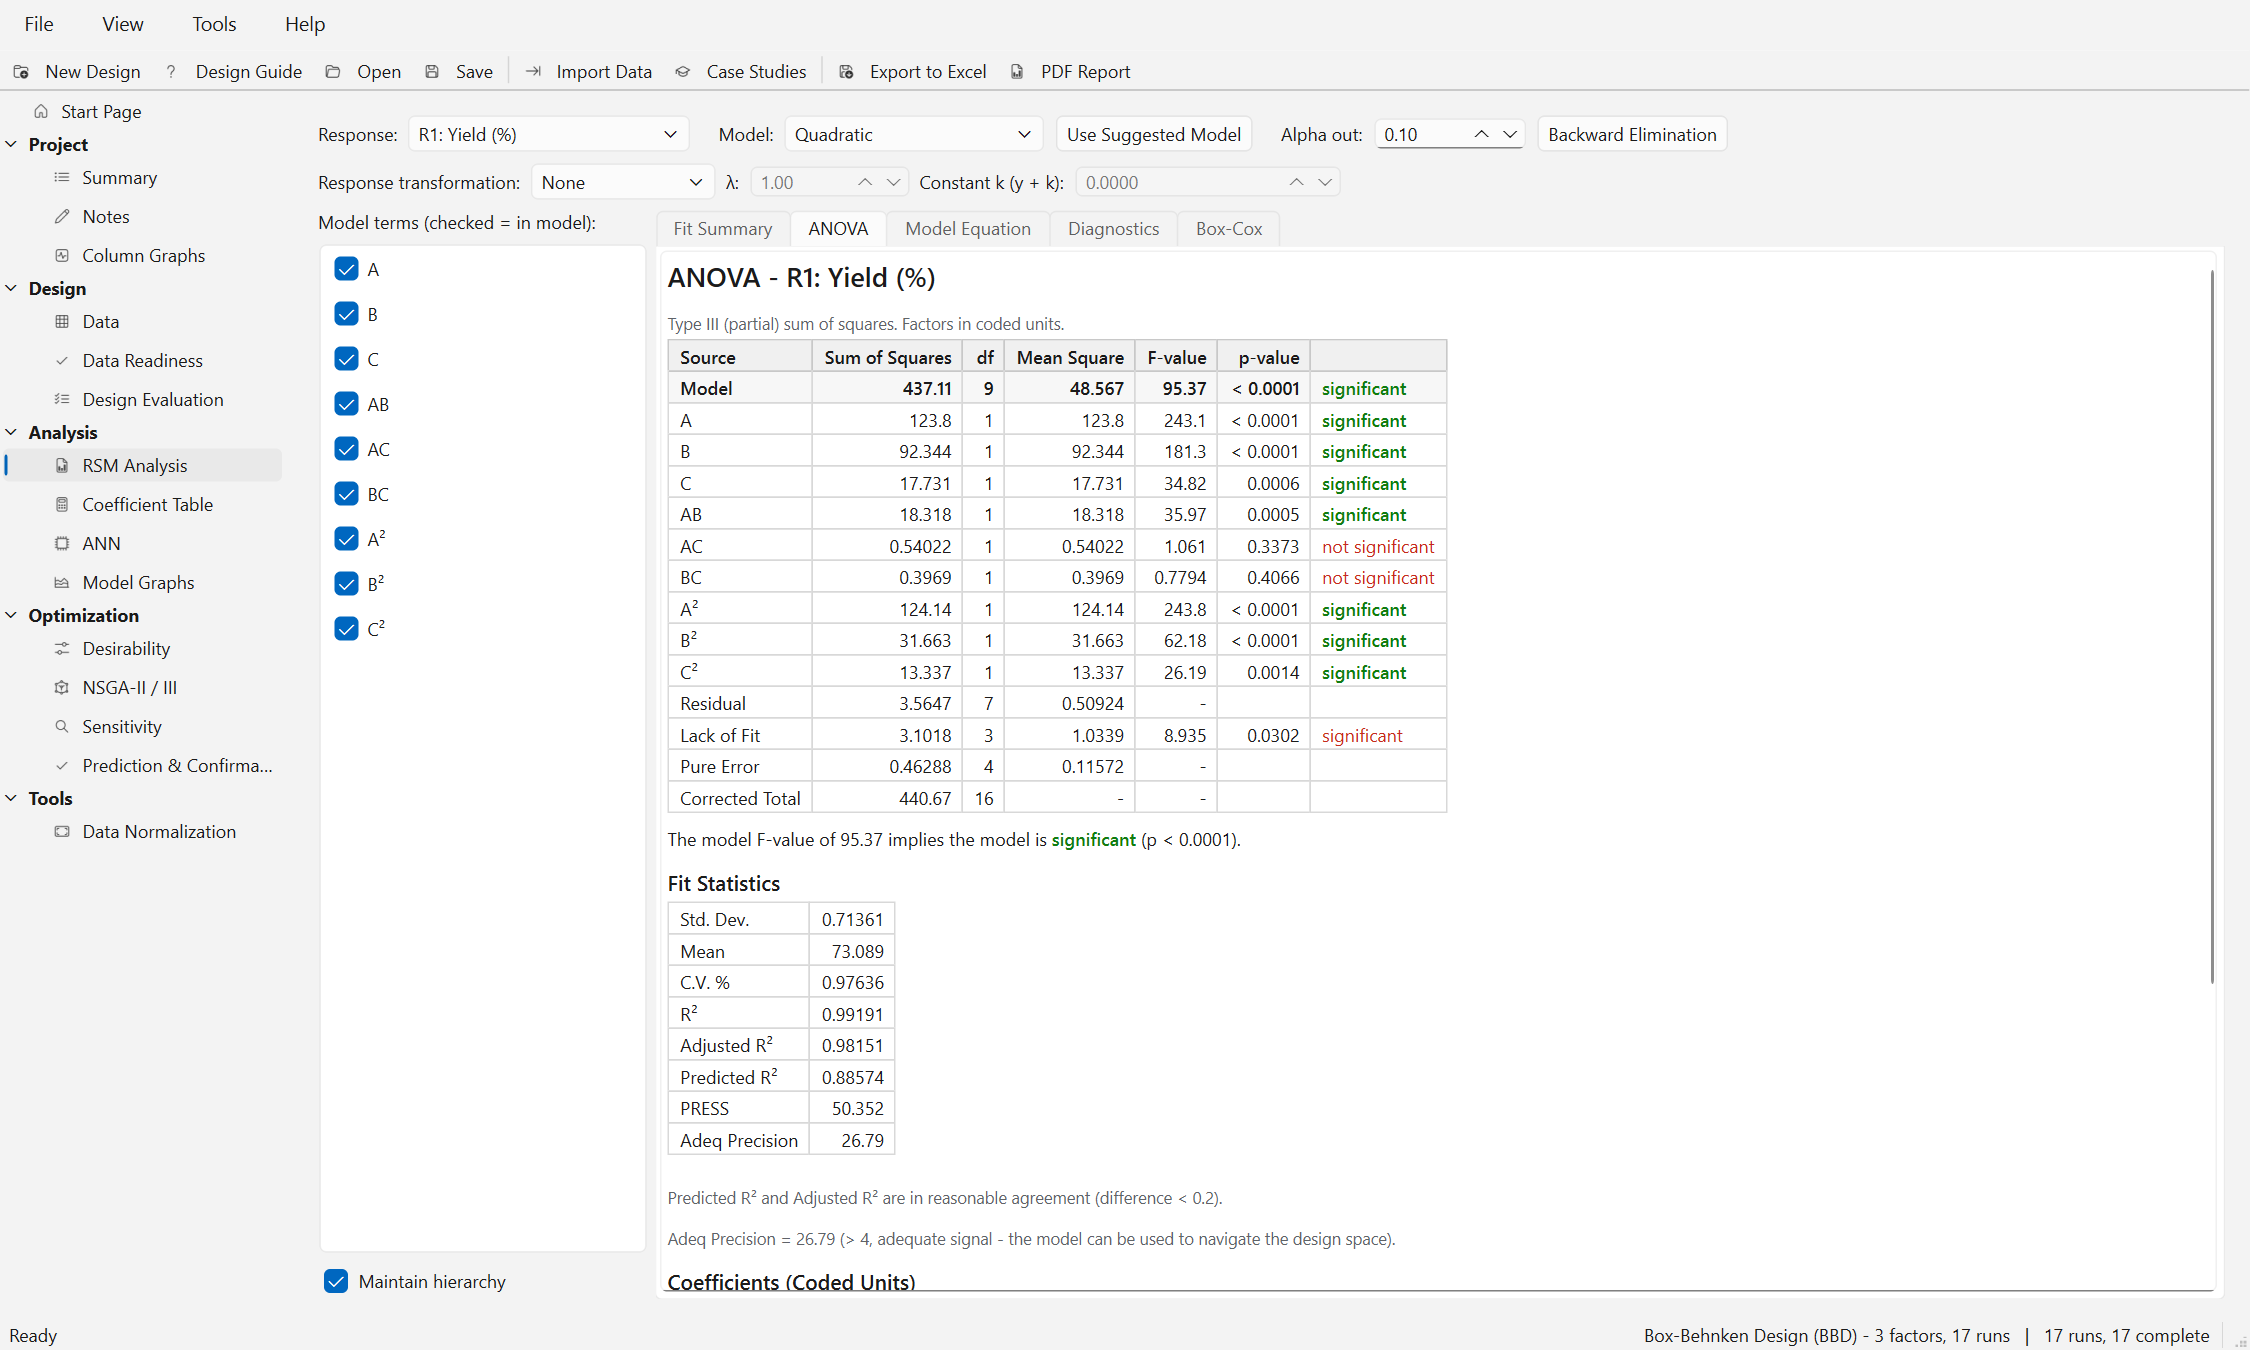
\includegraphics[width=\linewidth]{rsm_anova.png}
\caption{ANOVA sub-tab for Yield (Box-Behnken extraction case, quadratic model): Type III ANOVA with lack
of fit and pure error, model sentence, fit statistics and the notes below them.}
\label{fig:ch05-anova}
\end{figure}

\subsection*{Output and how to read it}
\begin{enumerate}
  \item Header notes: ``Type III (partial) sum of squares.'' and either ``Factors in coded units.'' or
        ``Scheffé model in pseudo-components.'', plus the transformation and the block note if present.
  \item The ANOVA table with the columns \ui{Source}, \ui{Sum of Squares}, \ui{df}, \ui{Mean Square},
        \ui{F-value}, \ui{p-value} and a verdict (``significant'' when $p<0.05$, otherwise ``not
        significant''). Green means good: $p<0.05$ for the model and the terms, $p\ge0.05$ for lack of
        fit. Rows: \ui{Block} (if any), \ui{Model}, \ui{Linear Mixture} (mixture models), one row per
        term, \ui{Residual}, \ui{Lack of Fit} and \ui{Pure Error} (when both have degrees of freedom) and
        \ui{Corrected Total}.
  \item A sentence on the model: ``The model F-value of \dots{} implies the model is significant (p
        \dots).'' or ``The model is not significant relative to noise.''
  \item \ui{Fit Statistics} (Table~\ref{tab:ch05-fitstats}) with two notes on the agreement of adjusted
        and predicted R² and on Adeq Precision.
  \item \ui{Coefficients (Coded Units)} or \ui{Coefficients (Pseudo-components)}: \ui{Term},
        \ui{Estimate}, \ui{df} (always 1 per column), \ui{Std. Error}, \ui{95\% CI Low}, \ui{95\% CI High}
        and \ui{VIF}. The p-values of the individual coefficients are on the \ui{Coefficient Table} page.
  \item Notes on mixture models, effect coding and the Shapiro-Wilk test of the residuals
        (Section~\ref{sec:ch05-diag}).
\end{enumerate}
p-values are printed with 4 decimals, or as ``$<$ 0.0001''.

\subsection*{Theory as implemented}
Let SST be the corrected total sum of squares and $\text{SSE}(S)$ the residual sum of squares of the model
with the column set $S$. The table is built as follows \citep{montgomery2017,myers2016}:
\begin{align}
  \text{SS}_{\text{Block}}&=\text{SST}-\text{SSE}(\mathbf 1,\text{blocks}), \label{eq:ch05-ssblock}\\
  \text{SS}_{\text{Model}}&=\text{SST}-\text{SS}_{\text{Block}}-\text{SSE}, \qquad
  F_{\text{Model}}=\frac{\text{SS}_{\text{Model}}/df_M}{\text{MSE}}, \label{eq:ch05-ssmodel}\\
  \text{SS}_t&=\text{SSE}(X\text{ without the columns of }t)-\text{SSE}, \qquad
  F_t=\frac{\text{SS}_t/df_t}{\text{MSE}}. \label{eq:ch05-sstype3}
\end{align}
$df_M$ is the number of term columns ($p-1$ for intercept-free mixture models) and $df_t$ the number of
columns of term $t$ (for example $L-1$ for a categoric main effect). Equation~\eqref{eq:ch05-sstype3} is
the partial (Type III) sum of squares: each term is tested after all other terms, so the term SS do not
add up to the model SS when the design is not orthogonal. The block SS in
\eqref{eq:ch05-ssblock} is sequential: blocks are removed first and the block columns stay in every reduced
model. Sequential sums of squares between model orders are used in the Fit Summary
(Equation~\ref{eq:ch05-seqF}).

\paragraph{Mixture models.} The linear blending terms are not tested one by one, because in a Scheffé model
they are not effects in the usual sense. They are tested together in the \ui{Linear Mixture} row:
\begin{equation}
  \text{SS}_{\text{lin}}=\text{SSE}(\mathbf 1+\text{non-linear terms})-\text{SSE}_{\text{full}},\qquad
  df_{\text{lin}}=q-1,
  \label{eq:ch05-linmix}
\end{equation}
with $q$ the number of linear blending columns. The note says ``In mixture models the linear terms are not
tested individually; they are tested together in the Linear Mixture row.''

\paragraph{Pure error and lack of fit.} Runs with identical coded settings (rounded to 6 decimals) in the
same block form a replicate group $g$. Then
\begin{equation}
  \text{SS}_{\text{PE}}=\sum_g\sum_{i\in g}(y_i-\bar y_g)^2,\quad df_{\text{PE}}=\sum_g(n_g-1),\qquad
  \text{SS}_{\text{LOF}}=\text{SSE}-\text{SS}_{\text{PE}},\quad df_{\text{LOF}}=(n-p)-df_{\text{PE}},
  \label{eq:ch05-lof}
\end{equation}
and $F_{\text{LOF}}=\text{MS}_{\text{LOF}}/\text{MS}_{\text{PE}}$ ($p=0$ is reported if the pure error is
exactly zero). Lack of fit is judged at $\alpha=0.05$ everywhere in the program.

\subsection*{Fit statistics}
Let $D=\text{SST}-\text{SS}_{\text{Block}}$ and $\bar y$ the mean of the (transformed) response.
Table~\ref{tab:ch05-fitstats} gives the exact formulas.

\begin{table}[htbp]\centering\small
\caption{Fit statistics on the ANOVA sub-tab ($n$ runs, $p$ columns, $df_M$ model df, $df_R=n-p$).}
\label{tab:ch05-fitstats}
\begin{tabularx}{\linewidth}{@{}l l X@{}}
\toprule
Label & Formula & Remark \\
\midrule
\ui{Std. Dev.} & $\sqrt{\text{MSE}}$ & residual standard deviation \\
\ui{Mean} & $\bar y$ & on the transformed scale \\
\ui{C.V. \%} & $100\sqrt{\text{MSE}}/|\bar y|$ & \\
\ui{R²} & $1-\text{SSE}/D$ & \\
\ui{Adjusted R²} & $1-\text{MSE}\big/\big(D/(df_M+df_R)\big)$ & penalizes the number of terms \\
\ui{Predicted R²} & $1-\text{PRESS}/D$ & not shown if a run has $h_{ii}>1-10^{-10}$ \\
\ui{PRESS} & $\sum_i\big(e_i/(1-h_{ii})\big)^2$ & leave-one-out prediction errors \citep{allen1974} \\
\ui{Adeq Precision} & $(\max_i\hat y_i-\min_i\hat y_i)\big/\sqrt{p\,\text{MSE}/n}$ & signal-to-noise ratio \\
\bottomrule
\end{tabularx}
\end{table}

PRESS uses the fact that the leave-one-out residual of run $i$ equals $e_i/(1-h_{ii})$, so no refitting is
needed \citep{allen1974}. Adeq Precision compares the range of the fitted values with the average standard
error of prediction at the design points: since $\sum_i h_{ii}=p$, the average prediction variance is
$p\,\text{MSE}/n$. The notes below the table read:
\begin{itemize}
  \item ``Predicted R² and Adjusted R² are in reasonable agreement (difference $<$ 0.2).'' or ``\dots
        differ by more than 0.2 - check for outliers or simplify the model.'' The program tests
        Adjusted R² minus Predicted R².
  \item ``Adeq Precision = \dots{} ($>$ 4, adequate signal - the model can be used to navigate the design
        space).'' or ``($\le$ 4, weak signal).''
\end{itemize}

The 95\% confidence interval of a coefficient is $\hat\beta_j\pm t_{0.975,\,n-p}\,\text{se}(\hat\beta_j)$.

\subsection*{What to do when a check fails}
\begin{itemize}
  \item \emph{Model not significant}: the factors explain no more than noise. Check the data entry,
        consider a lower order or accept that the factors have no effect in this range.
  \item \emph{Significant lack of fit}: try the next order, a transformation, or an ANN model; but first
        look at the size of the pure error (see the example).
  \item \emph{Adjusted and predicted R² differ by more than 0.2}: look for influential runs on the
        Diagnostics sub-tab and remove unnecessary terms.
\end{itemize}

\subsection*{Example: Box-Behnken extraction, Yield (quadratic)}
Figure~\ref{fig:ch05-anova} shows the result. The model has $F=95.37$ ($p<0.0001$). All main effects, AB
($F=35.97$, $p=0.0005$) and the three squares are significant; AC ($p=0.3373$) and BC ($p=0.4066$) are not.
The residual SS is 3.5647 on 7 df. Lack of fit is significant: $F=8.935$ on 3 and 4 df, $p=0.0302$. This
does not mean that the model is poor: the pure error comes from the 5 center points only and is very small
($\text{MS}_{\text{PE}}=0.1157$, a standard deviation of 0.34), while the residual standard deviation is
0.714. With so little pure-error information the lack-of-fit test reacts to small systematic deviations.
The other statistics are Std.\ Dev.\ 0.71361, Mean 73.089, C.V.\ 0.976\%, R² 0.99191, Adjusted R² 0.98151,
Predicted R² 0.88574 (PRESS 50.35) and Adeq Precision 26.79. Adjusted and predicted R² differ by 0.096, so
they agree. The coefficient table gives, for example, $A=3.9337$ with standard error 0.2523.

\subsection*{Example: mixture}
For \emph{Edible Film Formulation (Mixture)}, Tensile Strength, quadratic Scheffé model: Model $F=415.76$,
Linear Mixture SS 74.75 on 2 df ($F=561.0$), AB $F=96.56$, AC $F=212.5$, BC $F=6.19$ ($p=0.0377$), lack of
fit $p=0.0993$ (not significant), R² 0.99617, Adjusted R² 0.99377, Predicted R² 0.99122.

\begin{figure}[htbp]\centering
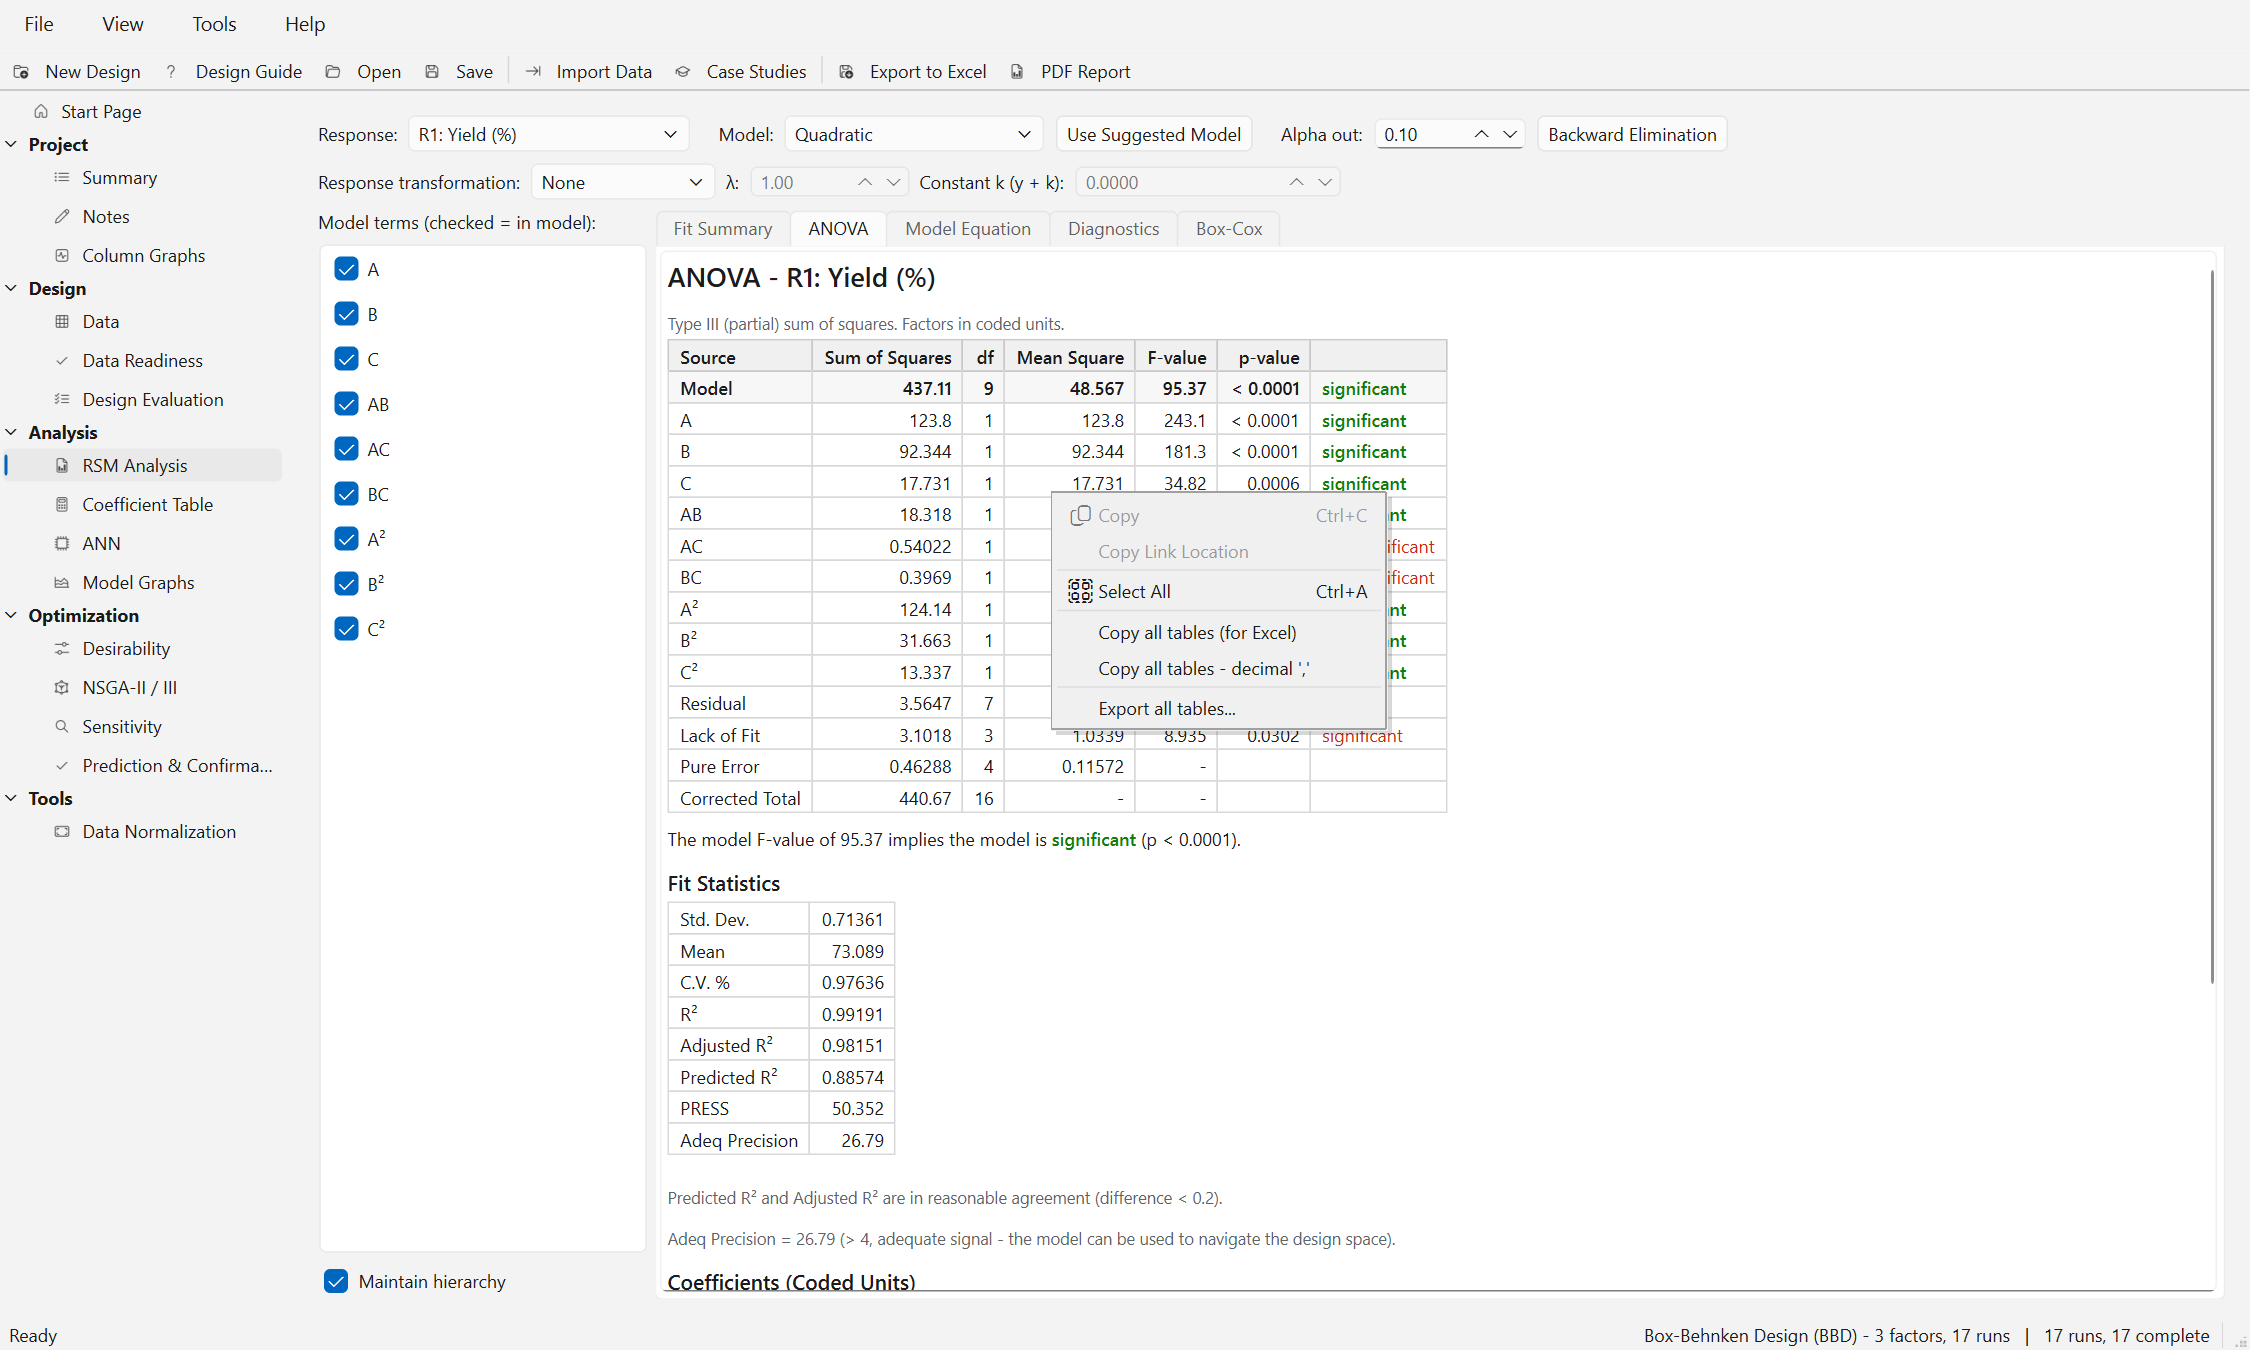
\includegraphics[width=0.75\linewidth]{report_context_menu.png}
\caption{Right-click menu of a report sub-tab: copy all tables to Excel (with either decimal separator) or
export them to a file.}
\label{fig:ch05-reportmenu}
\end{figure}

\subsection*{Data export}
Right-click any report sub-tab (Fit Summary, ANOVA, Model Equation, GLM or REML) for
\ui{Copy all tables (for Excel)}, \ui{Copy all tables - decimal ','} and \ui{Export all tables\dots}
(Figure~\ref{fig:ch05-reportmenu}). The export writes one Excel sheet per table, or a CSV file.

\section{Model equation}\label{sec:ch05-equation}

\subsection*{Purpose}
The \ui{Model Equation} sub-tab writes the fitted model as an equation that can be used outside the
program.

\begin{figure}[htbp]\centering
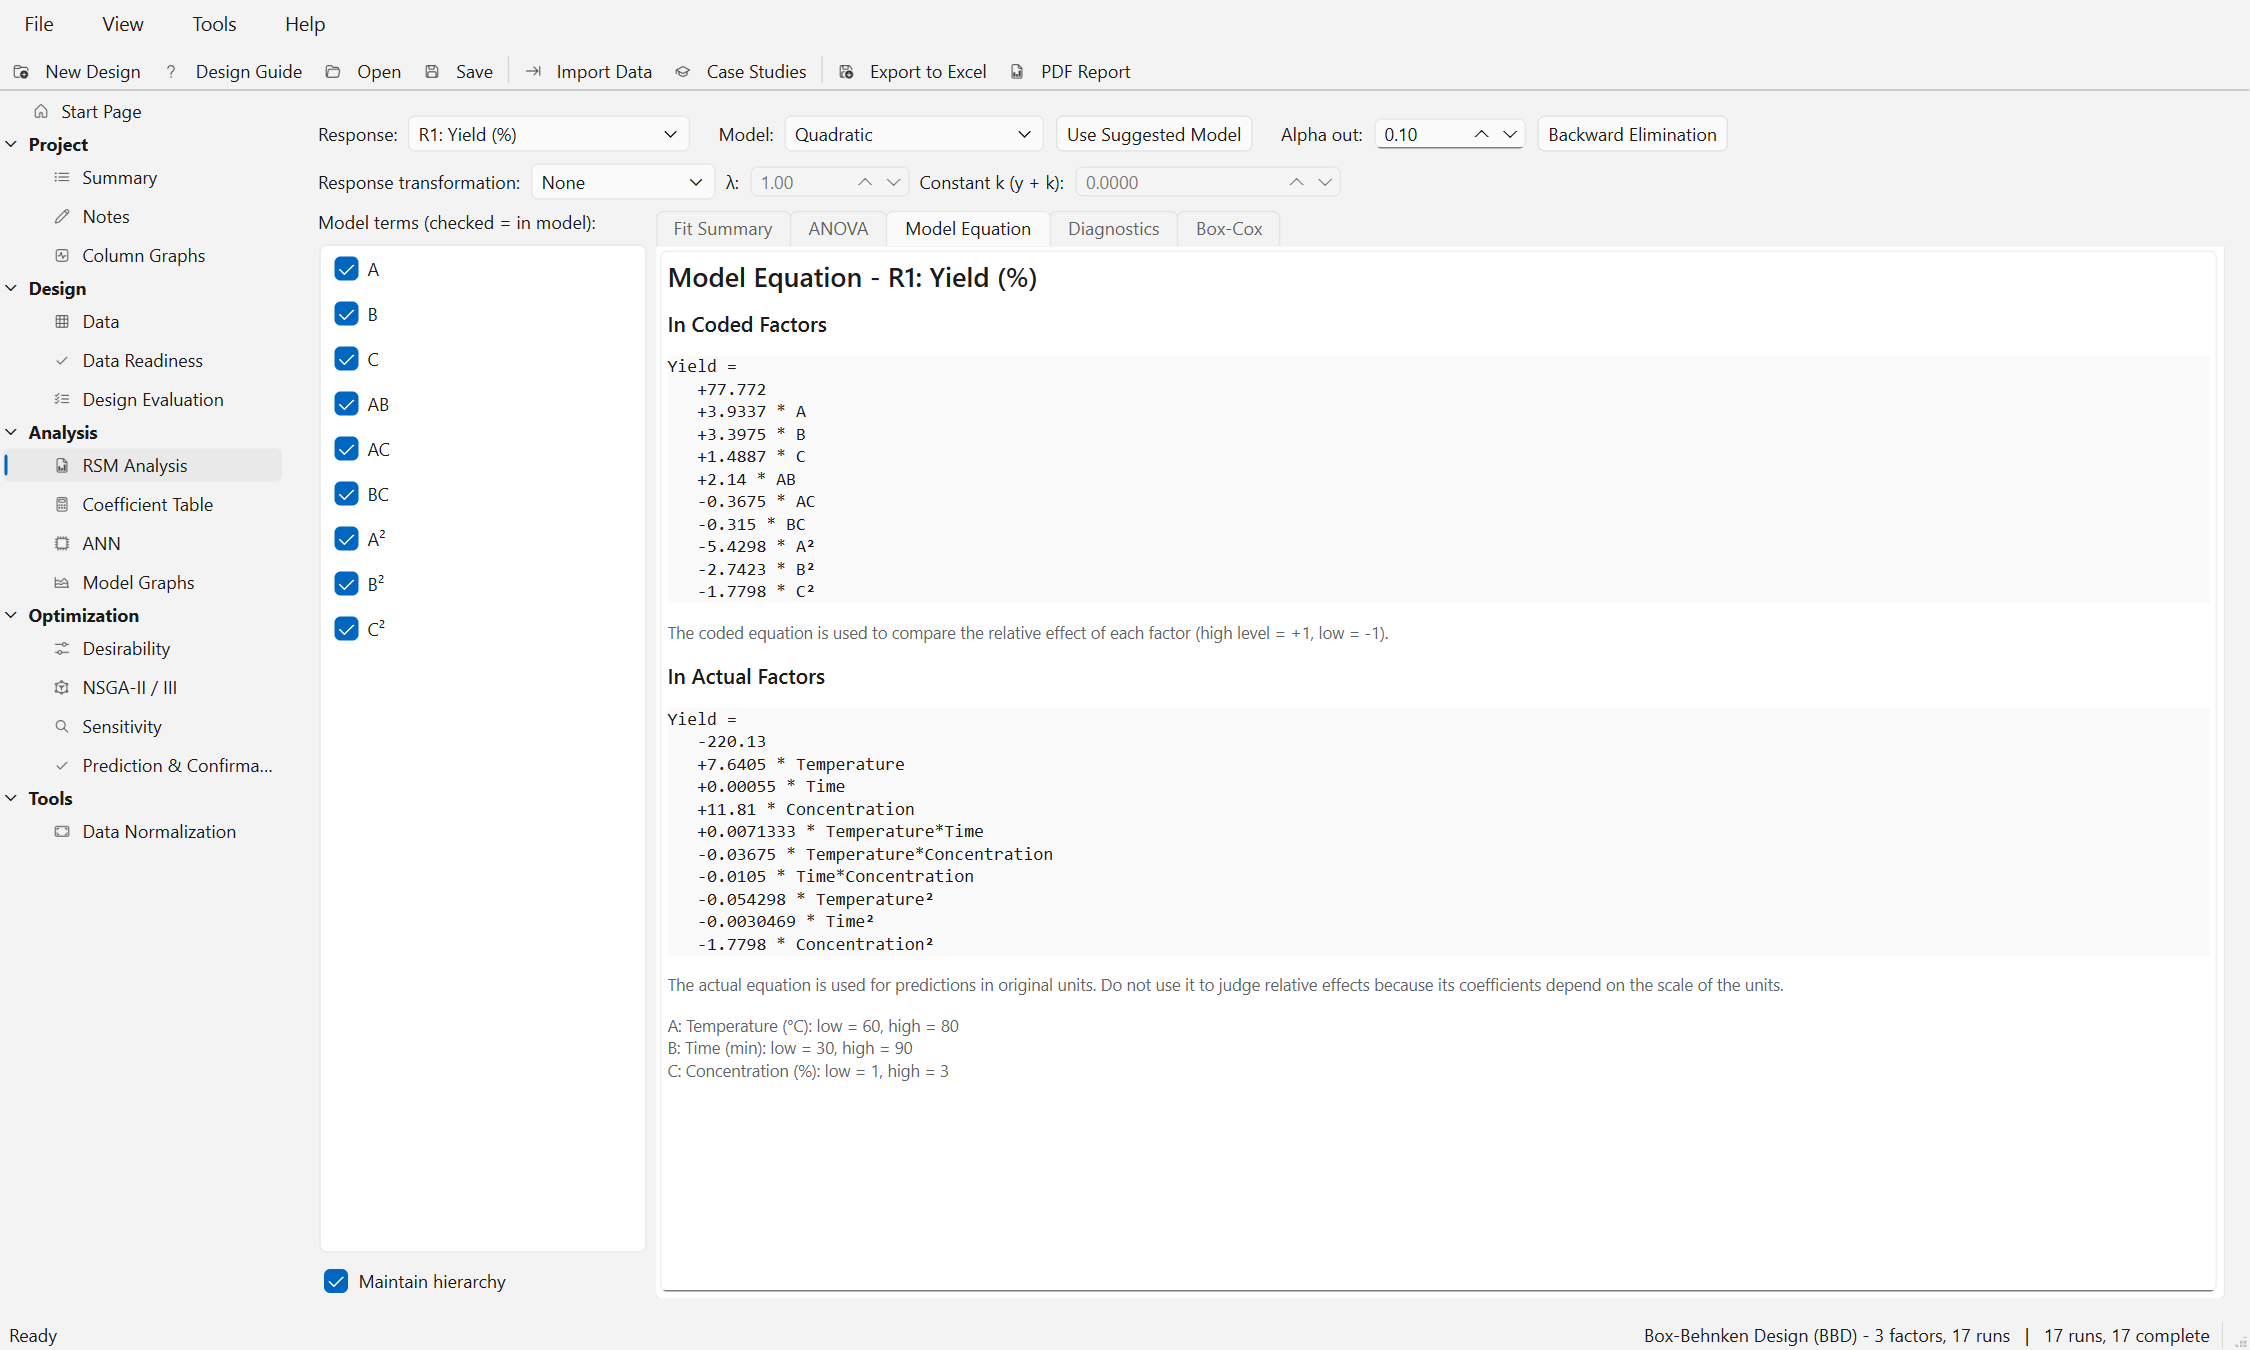
\includegraphics[width=\linewidth]{rsm_equation.png}
\caption{Model Equation sub-tab for Yield: the equation in coded factors and in actual factors.}
\label{fig:ch05-equation}
\end{figure}

\subsection*{Output and how to read it}
\begin{itemize}
  \item \ui{In Coded Factors}: the coefficients for factors coded $-1$ to $+1$. Note: ``The coded
        equation is used to compare the relative effect of each factor (high level = +1, low = -1).''
  \item \ui{In Actual Factors}: the same model in the original units, one block per combination of
        categoric levels (for example \ui{In Actual Factors - Solvent = Methanol}). Note: ``The actual
        equation is used for predictions in original units. Do not use it to judge relative effects
        because its coefficients depend on the scale of the units.''
  \item Mixture designs show \ui{In Pseudo-components}, with the note ``Pseudo-component: x = (amount
        $-$ lower limit) / (total $-$ $\Sigma$ lower limits). Linear coefficients = predicted response
        of the pure blends (vertices).'' \ui{In Actual Components} is shown only when every lower limit is
        0 and the design is not combined; otherwise a note says to use the pseudo-component equation. For
        combined mixture-process designs the note gives the reason: ``The equation in actual units is not
        given for combined mixture-process designs: the model crosses the mixture terms with the process
        terms, and the conversion to actual units is only done for mixture models without process factors.
        Use the equation above (pseudo-components, process factors coded $-1$ to $+1$).''
  \item The left-hand side shows the transformation, for example \ui{Ln(Yield)}, \ui{Sqrt(Yield)},
        \ui{(Yield +5)} for a constant $k=5$, \ui{logit(p Germinated)} for logistic and
        \ui{ln($\lambda$ \dots)} for Poisson regression.
  \item A legend lists the factor ranges (and the mixture total). With blocks: ``The equation applies to
        the average of all blocks.''
\end{itemize}

\subsection*{Theory as implemented}
Substituting \eqref{eq:ch05-coding} as $z_j=a_jx_j+b_j$ with $a_j=1/h_j$ and $b_j=-c_j/h_j$ into each
monomial and expanding binomially,
\begin{equation}
  \prod_j z_j^{e_j}=\prod_j\sum_{m=0}^{e_j}\binom{e_j}{m}a_j^{m}b_j^{\,e_j-m}x_j^{m},
  \label{eq:ch05-coded2actual}
\end{equation}
gives the actual coefficients. Categoric columns are first replaced by their values at the chosen level
(+1, $-1$ or 0, Equation~\ref{eq:ch05-effectcode}). For mixtures with all lower limits 0 the actual
coefficient of a term of degree $d$ is $\beta/T^{d}$.

\subsection*{Example}
For Yield of the Box-Behnken case (Figure~\ref{fig:ch05-equation}):
\begin{multline*}
\text{Yield}=77.772+3.9337A+3.3975B+1.4887C+2.14AB-0.3675AC\\
-0.315BC-5.4298A^2-2.7423B^2-1.7798C^2
\end{multline*}
in coded units, and in actual units (Temperature $T$, Time $t$, Concentration $c$)
\begin{multline*}
\text{Yield}=-220.13+7.6405\,T+0.00055\,t+11.81\,c+0.0071333\,Tt-0.03675\,Tc\\
-0.0105\,tc-0.054298\,T^2-0.0030469\,t^2-1.7798\,c^2.
\end{multline*} The coefficient of Time in actual units is
almost zero although Time is the second most important factor: actual coefficients cannot be compared.
For the categoric case the three actual equations differ only in the intercept and in the coefficients
of Temperature and Time, for example intercept $-48.211$ (Ethanol), $-51.117$ (Methanol) and $-51.911$
(Acetone).

\section{Backward elimination}\label{sec:ch05-backward}

\subsection*{Purpose}
Backward elimination removes terms that do not contribute significantly, to obtain a smaller model with
better prediction properties.

\subsection*{How to use}
\begin{enumerate}
  \item Choose the starting model (order and terms).
  \item Set \ui{Alpha out:} (default 0.10).
  \item Click \ui{Backward Elimination}. The term list shows the result; undo by selecting the order again
        in \ui{Model:} (this restores all terms).
\end{enumerate}

\subsection*{Rule as implemented}
\begin{enumerate}
  \item Fit the current terms. If the residual df is 0, stop (a saturated model is not reduced).
  \item Candidates are the terms with a p-value larger than $\alpha_{\text{out}}$: the Type III F test for
        least squares, the likelihood-ratio test for GLM, the Wald F test for REML.
  \item A term is not a candidate if it is a linear mixture term or, when \ui{Maintain hierarchy} is checked
        (the default), if it is contained in another term that is still in the model. With the check box
        cleared, any term with $p>\alpha_{\text{out}}$ can be removed, and the result may be a
        non-hierarchical model.
  \item Remove the candidate with the largest p-value, refit and repeat until no candidate is left.
\end{enumerate}
Because the p-values change after each removal, removing terms one at a time is safer than removing all
non-significant terms at once.

\subsection*{Examples}
\begin{itemize}
  \item Box-Behnken, Yield, quadratic, $\alpha_{\text{out}}=0.10$: BC and then AC are removed; the model
        A, B, C, AB, A², B², C² remains. For Purity the same procedure removes B² first ($p=0.9745$
        in the full model) and then AC and BC.
  \item Germination (logistic): only B² is removed (likelihood-ratio $p=0.5312$); AB stays because its
        $p=0.0622$ is below 0.10.
  \item Oven hardness (split-plot): AC and BC are removed; A, B, C, AB remain.
\end{itemize}

\section{Response transformations and Box-Cox}\label{sec:ch05-transform}

\subsection*{Purpose}
A transformation can make the residual variance constant, the residuals more normal and the model simpler.
The Box-Cox plot shows which power transformation the data support.

\subsection*{Transformations}
The constant $k$ (\ui{Constant k (y + k):}) is added first, $v=y+k$. Then:

\begin{center}\small
\begin{tabular}{@{}llll@{}}
\toprule
Option & Forward & Requirement & Equation label \\
\midrule
None & $y$ & -- & \ui{Yield} \\
Square root & $\sqrt v$ & all $v\ge0$ & \ui{Sqrt(Yield)} \\
Natural log (ln) & $\ln v$ & all $v>0$ & \ui{Ln(Yield)} \\
Base 10 log & $\log_{10}v$ & all $v>0$ & \ui{Log10(Yield)} \\
Inverse (1/y) & $1/v$ & all $v>0$ & \ui{1/(Yield)} \\
Power (y\^{}$\lambda$) & $v^\lambda$ ($\ln v$ if $\lambda=0$) & all $v>0$ & \ui{(Yield)\^{}$\lambda$} \\
\bottomrule
\end{tabular}
\end{center}

All statistics (ANOVA, R², Std.\ Dev., Mean) refer to the transformed scale. Predictions, confidence and
prediction intervals are computed on the transformed scale, back-transformed (the inverse power uses
$\text{sign}(z)|z|^{1/\lambda}$), $k$ is subtracted, and the interval limits are sorted (the inverse
transformation reverses their order). Graphs and optimization therefore work in the original units.
The transformation box is disabled for binomial and Poisson responses.

\subsection*{How to use the Box-Cox sub-tab}
\begin{enumerate}
  \item Select the model first; the Box-Cox plot is computed for the current terms (and blocks).
  \item If any response value is $\le0$, choose a transformation and enter a constant $k$ that makes all
        $y+k>0$; the plot then refers to $y+k$ (the x-axis label shows ``transform of y +k'').
  \item Read the recommendation below the plot and click \ui{Apply Recommendation} to set the
        transformation (and $\lambda$ for Power). The constant $k$ is not changed.
\end{enumerate}

\begin{figure}[htbp]\centering
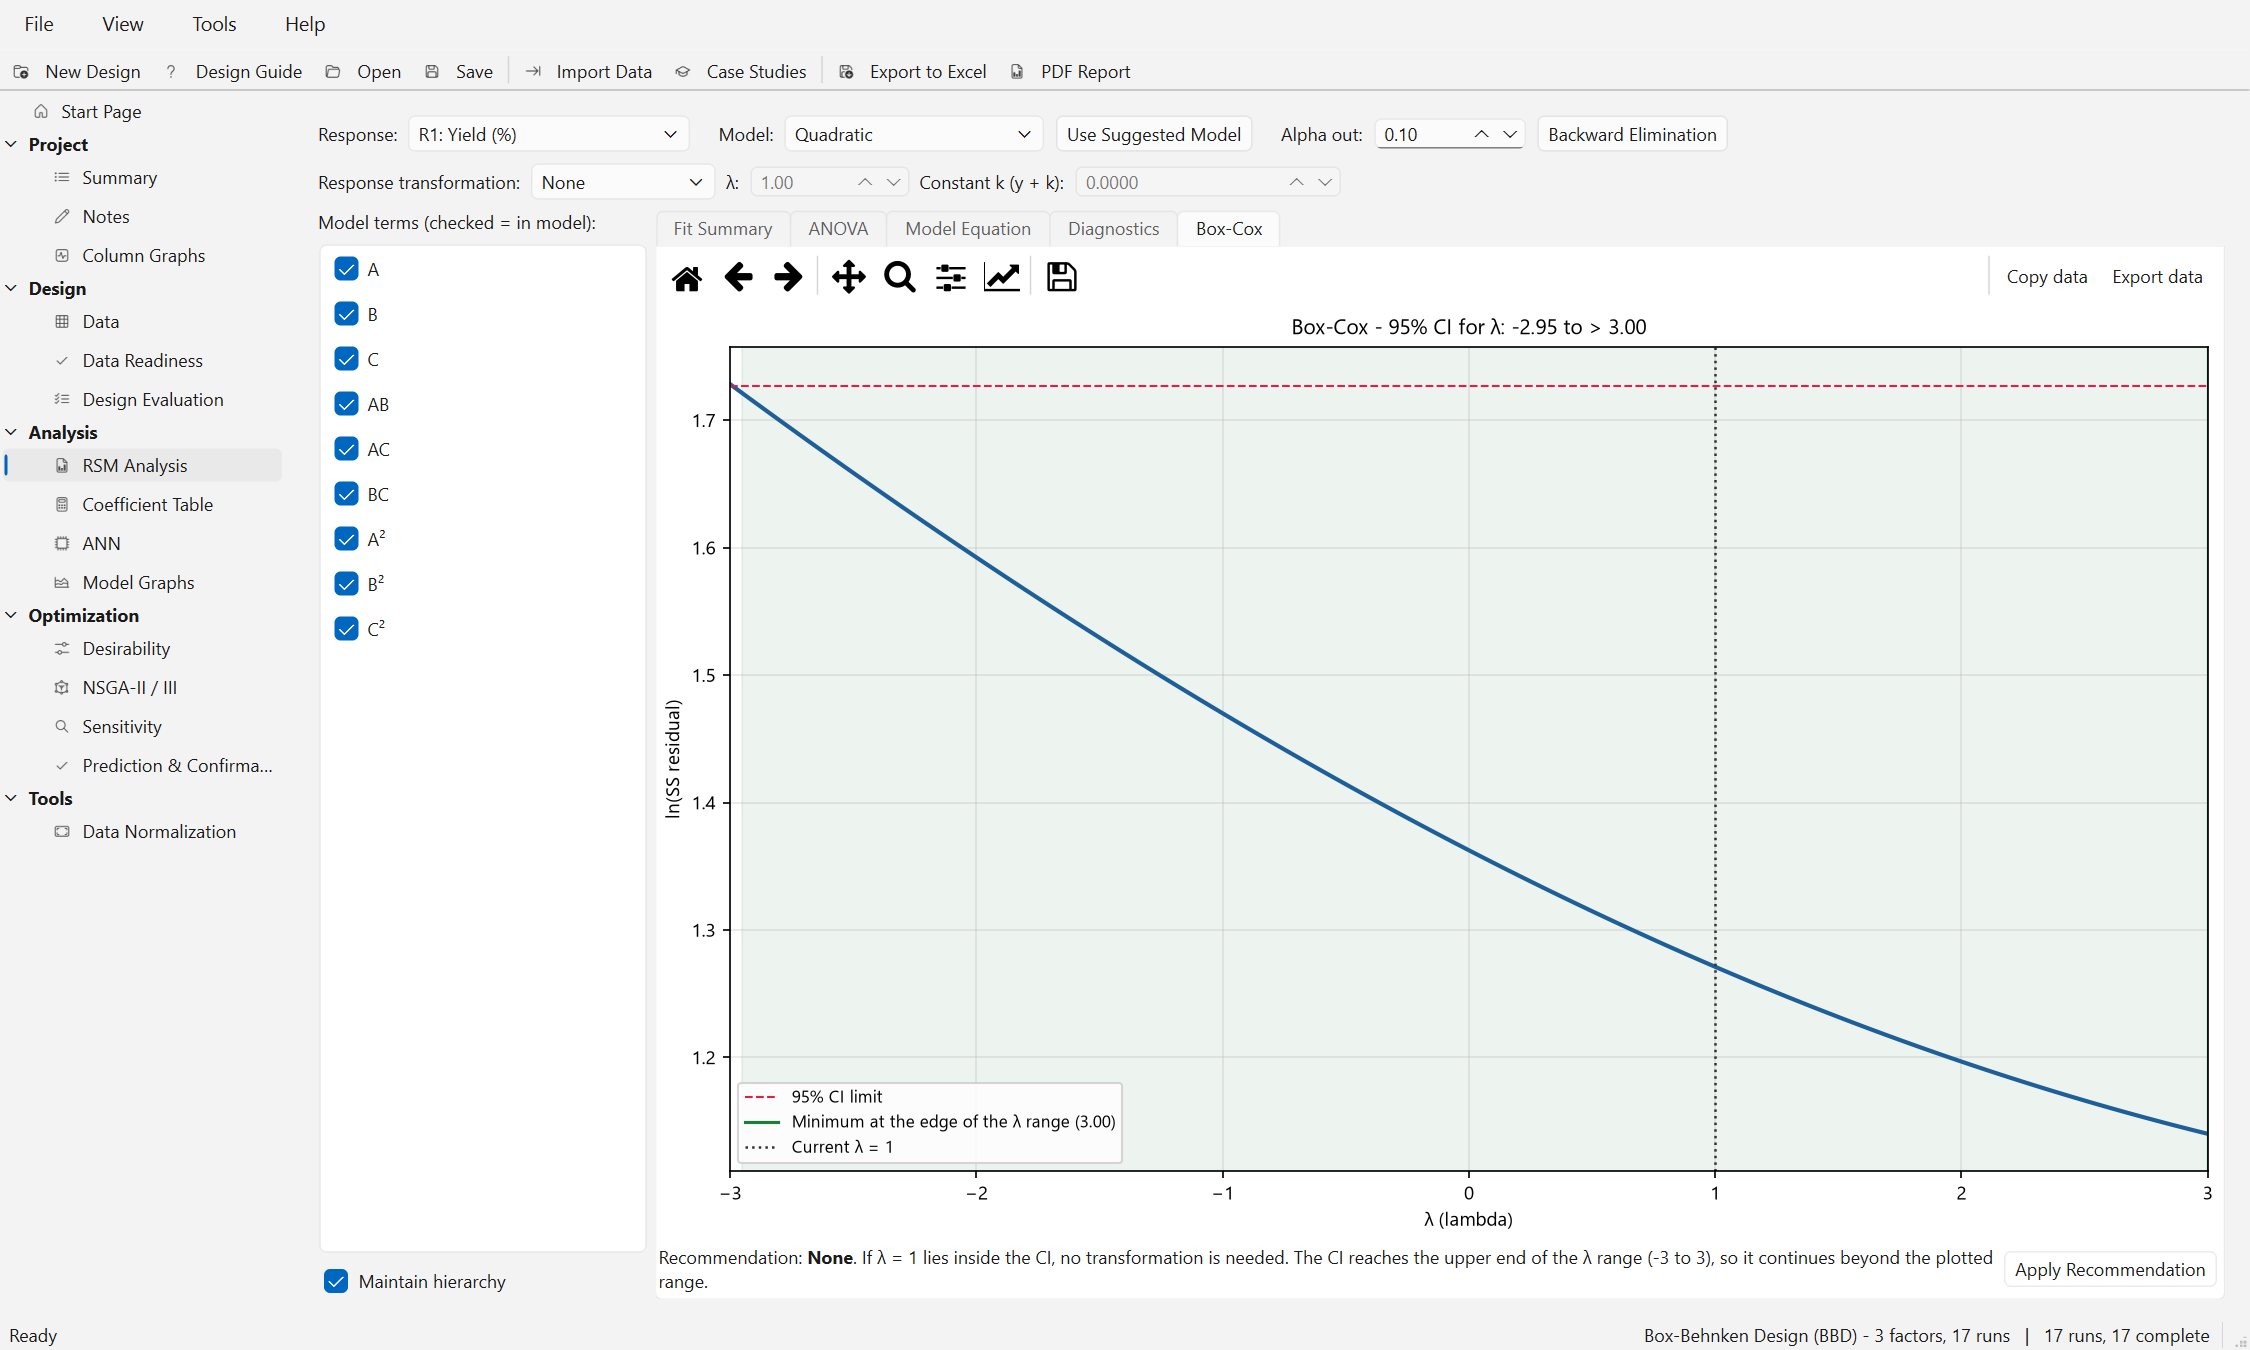
\includegraphics[width=\linewidth]{rsm_boxcox.png}
\caption{Box-Cox sub-tab for Yield (Box-Behnken case): ln(SS residual) against $\lambda$ with the 95\%
limit, the confidence band and the recommendation ``None''.}
\label{fig:ch05-boxcox}
\end{figure}

\subsection*{Theory as implemented}
For each $\lambda$ on the grid $-3,-2.95,\dots,3$ (121 values) the scaled power transformation
\begin{equation}
  w^{(\lambda)}=\begin{cases}\dfrac{v^\lambda-1}{\lambda\,\dot v^{\lambda-1}}, & \lambda\neq0,\\[1ex]
  \dot v\ln v, & \lambda=0,\end{cases}\qquad \dot v=\exp\Big(\frac1n\sum\ln v_i\Big),
  \label{eq:ch05-boxcox}
\end{equation}
is regressed on the current model matrix, and the residual sum of squares $\text{SS}(\lambda)$ is computed
\citep{boxcox1964}. The geometric mean $\dot v$ makes the SS comparable across $\lambda$, so maximizing the
likelihood is the same as minimizing $\text{SS}(\lambda)$: the profile log-likelihood is
$\ell(\lambda)=-\tfrac n2\ln\text{SS}(\lambda)+\text{const}$. The plot shows $\ln\text{SS}(\lambda)$; the
best $\lambda$ is the grid minimum. The approximate 95\% confidence interval contains all $\lambda$ with
\begin{equation}
  \ln\text{SS}(\lambda)\le\ln\text{SS}(\hat\lambda)+\ln\!\Big(1+\frac{t^2_{0.975,\nu}}{\nu}\Big),
  \qquad \nu=n-p,
  \label{eq:ch05-boxcoxci}
\end{equation}
which is the usual $\text{SS}^{*}=\text{SS}(\hat\lambda)(1+t^2_{\alpha/2,\nu}/\nu)$ rule
\citep{montgomery2017,boxcox1964}.

\paragraph{Recommendation rule.}
\begin{enumerate}
  \item If $\lambda=1$ lies in the CI: \emph{None}.
  \item Otherwise the first of $\lambda=0.5$ (\emph{Square root}), $0$ (\emph{Natural log}) and $-1$
        (\emph{Inverse}) that lies in the CI.
  \item Otherwise \emph{Power} with the best $\lambda$ rounded to 2 decimals, unless the minimum lies at the
        edge of the grid; then no recommendation is given.
\end{enumerate}

\paragraph{Plot and messages.} The blue curve is $\ln\text{SS}$; the dashed red line labeled ``95\% CI
limit'' is the threshold of \eqref{eq:ch05-boxcoxci} and the green band the CI. A green vertical line marks
``Best $\lambda$ = \dots'' or, when the minimum is at the end of the grid, ``Minimum at the edge of the
$\lambda$ range (\dots)''. A dotted line marks the current $\lambda$ (1 for none, 0.5, 0 for both logs, $-1$,
or the power). The title reads ``Box-Cox - 95\% CI for $\lambda$: lo to hi''; a limit that reaches the end of
the grid is written ``$<$ -3.00'' or ``$>$ 3.00''. The text below the plot gives the recommendation and adds
``The CI reaches the upper end of the $\lambda$ range (-3 to 3), so it continues beyond the plotted range.''
when this happens. If the minimum is at the edge and no standard value is in the CI, the text explains that
no reliable $\lambda$ can be given and advises to check the model (lack of fit, outliers) first. Box-Cox is
not available for binomial, Poisson or split-plot responses (``Box-Cox is not available for this
response.''), and needs at least 3 values with all $y+k>0$.

\subsection*{Examples}
\begin{itemize}
  \item Box-Behnken, Yield (Figure~\ref{fig:ch05-boxcox}): the curve is very flat, the CI is $-2.95$ to
        $>3.00$ and the minimum is at the upper edge ($\lambda=3$). Because $\lambda=1$ is inside the CI,
        the recommendation is \emph{None}. The response varies only between 64 and 78\%, so the data carry
        almost no information about $\lambda$.
  \item Edible film, Tensile Strength: best $\lambda=1.10$, CI 0.15 to 2.00, recommendation \emph{None}.
  \item Fermentation screening, Biomass (2FI): best $\lambda=0.90$, CI 0.45 to 1.35, recommendation
        \emph{None}.
\end{itemize}

\section{Residual diagnostics}\label{sec:ch05-diag}

\subsection*{Purpose}
The \ui{Diagnostics} sub-tab checks the assumptions of the analysis (normal, independent residuals with
constant variance) and finds runs that are outliers or have a large influence on the model.

\begin{figure}[htbp]\centering
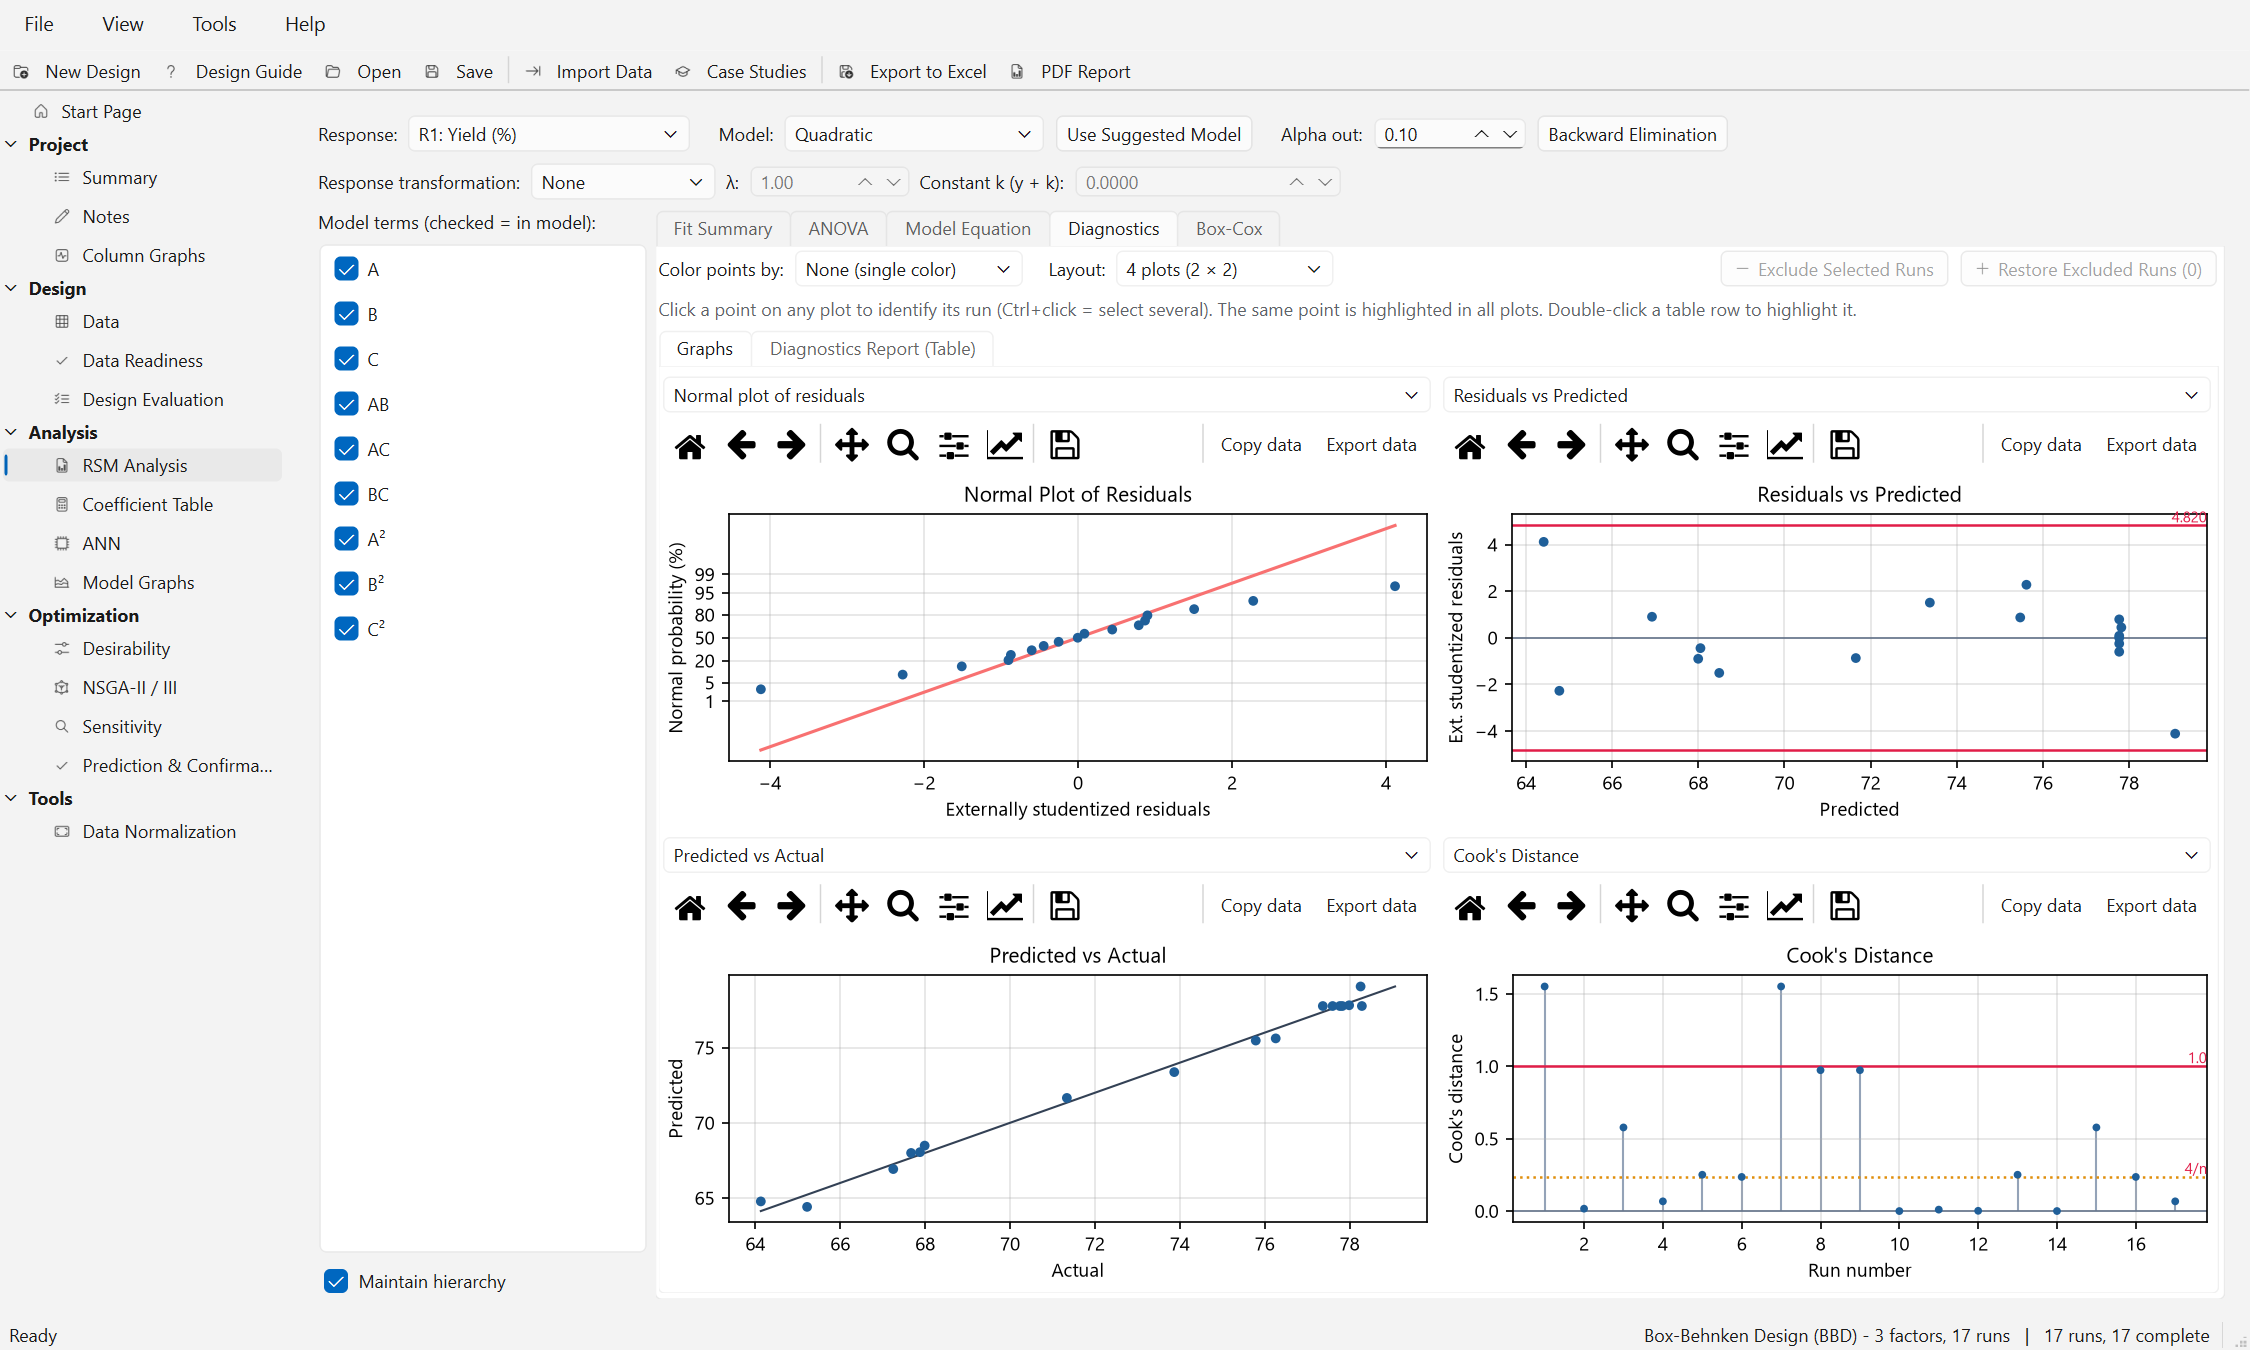
\includegraphics[width=\linewidth]{rsm_diagnostics.png}
\caption{Diagnostics sub-tab (Box-Behnken case, Yield) with the default four plots: normal plot, residuals
versus predicted with the Bonferroni limits, predicted versus actual and Cook's distance.}
\label{fig:ch05-diag}
\end{figure}

\subsection*{How to use}
\begin{enumerate}
  \item Choose the plots: each of the four panels has its own selector (Table~\ref{tab:ch05-diagplots}) and
        its own plot toolbar.
  \item Optionally color the points with \ui{Color points by:} and change the number of panels with
        \ui{Layout:}.
  \item Click a point to identify its run; the same run is circled and labeled in every plot, and the text
        above the plots shows its actual and predicted value, externally studentized residual, leverage and
        Cook's distance. Ctrl+click (or Shift+click) selects several runs. Clicking away from the points
        clears the selection. Clicks are ignored while the zoom or pan tool of the plot toolbar is active.
  \item Open the inner tab \ui{Diagnostics Report (Table)} for all numbers. Double-click a row to highlight
        that run in the plots.
  \item To leave runs out of the analysis, select them and click \ui{Exclude Selected Runs}; restore them
        with \ui{Restore Excluded Runs (N)}.
\end{enumerate}

\begin{table}[htbp]\centering\small
\caption{Options of the Diagnostics sub-tab.}\label{tab:ch05-diagopts}
\begin{tabularx}{\linewidth}{@{}>{\raggedright\arraybackslash}p{2.4cm} >{\raggedright\arraybackslash}p{3.8cm} >{\raggedright\arraybackslash}p{3.0cm} X@{}}
\toprule
Option & Values & Default & Meaning \\
\midrule
\ui{Color points by:} & None (single color), each factor, Run order, Predicted value & None & Numeric values use a continuous color scale with a color bar; categoric factors one color per level with a legend. \\
\ui{Layout:} & 4 plots (2 $\times$ 2), 2 plots side by side, 1 large plot & 4 plots & Number of panels shown. \\
Panel selector & see Table~\ref{tab:ch05-diagplots} & Normal plot, Residuals vs Predicted, Predicted vs Actual, Cook's Distance & Plot in each panel. \\
\bottomrule
\end{tabularx}
\end{table}

\begin{table}[htbp]\centering\small
\caption{Diagnostic plots available in each panel.}\label{tab:ch05-diagplots}
\begin{tabularx}{\linewidth}{@{}>{\raggedright\arraybackslash}p{3.4cm} X@{}}
\toprule
Plot & Content \\
\midrule
Normal plot of residuals & Sorted externally studentized residuals against $\Phi^{-1}((i-0.5)/n)$, axis in \% (1 to 99, or 0.1 to 99.9 for $n\ge200$), with the line $y=x$. Needs 3 valid points. \\
Residuals vs Predicted & Externally studentized residuals against $\hat y$ (GLM: against the linear predictor, axis ``Linear predictor (logit scale)'' or ``(log scale)''), with the zero line and the $\pm$Bonferroni limits labeled with their value. With a response transformation $\hat y$ is on the transformed scale and the axis reads ``Predicted (transformed scale)''. \\
Residuals vs Run Order & The same residuals against the run number, joined by a line (up to 400 runs). \\
Residuals vs \emph{factor} & One plot per factor; categoric levels are jittered by $\pm0.12$. \\
Predicted vs Actual & Fitted against observed values with the 45° line (transformed scale if a transformation is used; GLM: observed proportion or count against fitted probability or mean). \\
Cook's Distance & Stems against run number with a line at 1.0 and a dotted line at $4/n$ (not for REML). \\
Leverage & Stems with a line at $2p/n$. \\
DFFITS & Stems with lines at $\pm2\sqrt{p/n}$ (not for REML). \\
Histogram of residuals & Density histogram of the externally studentized residuals ($\min(40,\max(8,\lfloor n/5\rfloor))$ bins) with the standard normal density. \\
DFBETAS - \emph{term} & One plot per coefficient, lines at $\pm2/\sqrt n$ (least squares only). \\
\bottomrule
\end{tabularx}
\end{table}

\subsection*{Theory as implemented}
With $\nu=n-p$ residual degrees of freedom \citep{montgomery2017,myers2016}:
\begin{align}
  r_i&=\frac{e_i}{\sqrt{\text{MSE}(1-h_{ii})}} &&\text{(internally studentized)}, \label{eq:ch05-rint}\\
  t_i&=r_i\sqrt{\frac{\nu-1}{\nu-r_i^2}} &&\text{(externally studentized, needs } \nu>1), \label{eq:ch05-rext}\\
  D_i&=\frac{r_i^2}{p}\,\frac{h_{ii}}{1-h_{ii}} &&\text{(Cook's distance \citep{cook1977})}, \label{eq:ch05-cook}\\
  \text{DFFITS}_i&=t_i\sqrt{\frac{h_{ii}}{1-h_{ii}}}, && \label{eq:ch05-dffits}\\
  \text{DFBETAS}_{ij}&=\frac{\big[(X'X)^{-1}x_i\big]_j\,e_i/(1-h_{ii})}{s_{(i)}\sqrt{[(X'X)^{-1}]_{jj}}}
  && \text{\citep{belsley1980}}, \label{eq:ch05-dfbetas}
\end{align}
with $s_{(i)}^2=\big(\text{SSE}-e_i^2/(1-h_{ii})\big)/(\nu-1)$, the residual variance without run $i$.
The externally studentized residual is the residual of run $i$ divided by an error estimate that does not
use run $i$; under the model it follows a $t$ distribution with $\nu-1$ df. Runs with
$h_{ii}>1-10^{-10}$ (fitted exactly) get no studentized residual. DFBETAS measures how many standard errors
coefficient $j$ moves when run $i$ is deleted and is computed only for least-squares fits with $\nu>1$.

Limits used for the red cells and the plot lines:
\begin{center}\small
\begin{tabular}{@{}ll@{}}
\toprule
Statistic & Flagged when \\
\midrule
Ext.\ studentized residual & $|t_i|>t_{1-0.05/(2n),\,\nu-1}$ (Bonferroni outlier limit) \\
Leverage & $h_{ii}>2p/n$ \\
Cook's distance & $D_i>1$ (the plot also shows $4/n$) \\
DFFITS & $|\text{DFFITS}_i|>2\sqrt{p/n}$ \\
DFBETAS & $|\text{DFBETAS}_{ij}|>2/\sqrt n$ \\
\bottomrule
\end{tabular}
\end{center}

\paragraph{Normality: Shapiro-Wilk.} The ANOVA sub-tab reports the Shapiro-Wilk test of the raw residuals
\citep{shapiro1965} for $3\le n\le5000$: ``Shapiro-Wilk normality test of residuals: p = \dots{} (residuals
can be considered normal).'' when $p\ge0.05$, otherwise ``(residuals are not normal - consider a
transformation).'' With few runs the test has little power; the normal plot is more informative.

\paragraph{Independence: run order and Durbin-Watson.} Look at \ui{Residuals vs Run Order}: a trend or long
runs of residuals with the same sign suggest drift during the experiment. The Durbin-Watson statistic
$d=\sum_{i\ge2}(e_i-e_{i-1})^2/\sum_i e_i^2$ (residuals in run order, \citealp{durbin1950}) is not shown on
this page; it is computed on the \ui{Data Readiness} page, which warns when $d<1.4$, $d>2.6$ or the Spearman
trend of the residuals over the run order has $p<0.01$. Values near 2 mean no serial correlation.

\subsection*{Diagnostics report table}
The table (Figure~\ref{fig:ch05-diagtable}) has one row per analyzed run, sorted by run order, with the
columns \ui{Run}, \ui{Std}, \ui{Type}, \ui{Actual}, \ui{Predicted}, \ui{Residual}, \ui{Leverage},
\ui{Int. stud. resid.}, \ui{Ext. stud. resid.}, \ui{Cook's}, \ui{DFFITS} and one \ui{DFBETAS} column per
coefficient (least squares only). \ui{Actual} is in original units. With a response transformation the
predicted values and residuals are on the transformed scale, and the columns are then labeled
\ui{Predicted (transformed scale)} and \ui{Residual (transformed scale)}. For GLM responses the columns are \ui{Observed proportion} (or count),
\ui{Fitted probability} (or \ui{Fitted mean count}) and \ui{Deviance resid.}. Cells beyond the limits
are shaded red. The line above the table states the number of runs analyzed and excluded, each limit and
how many runs exceed it. Right-click the table to copy it (\ui{Copy entire table (for Excel)}, with either
decimal separator) or \ui{Export table\dots}.

\begin{figure}[htbp]\centering
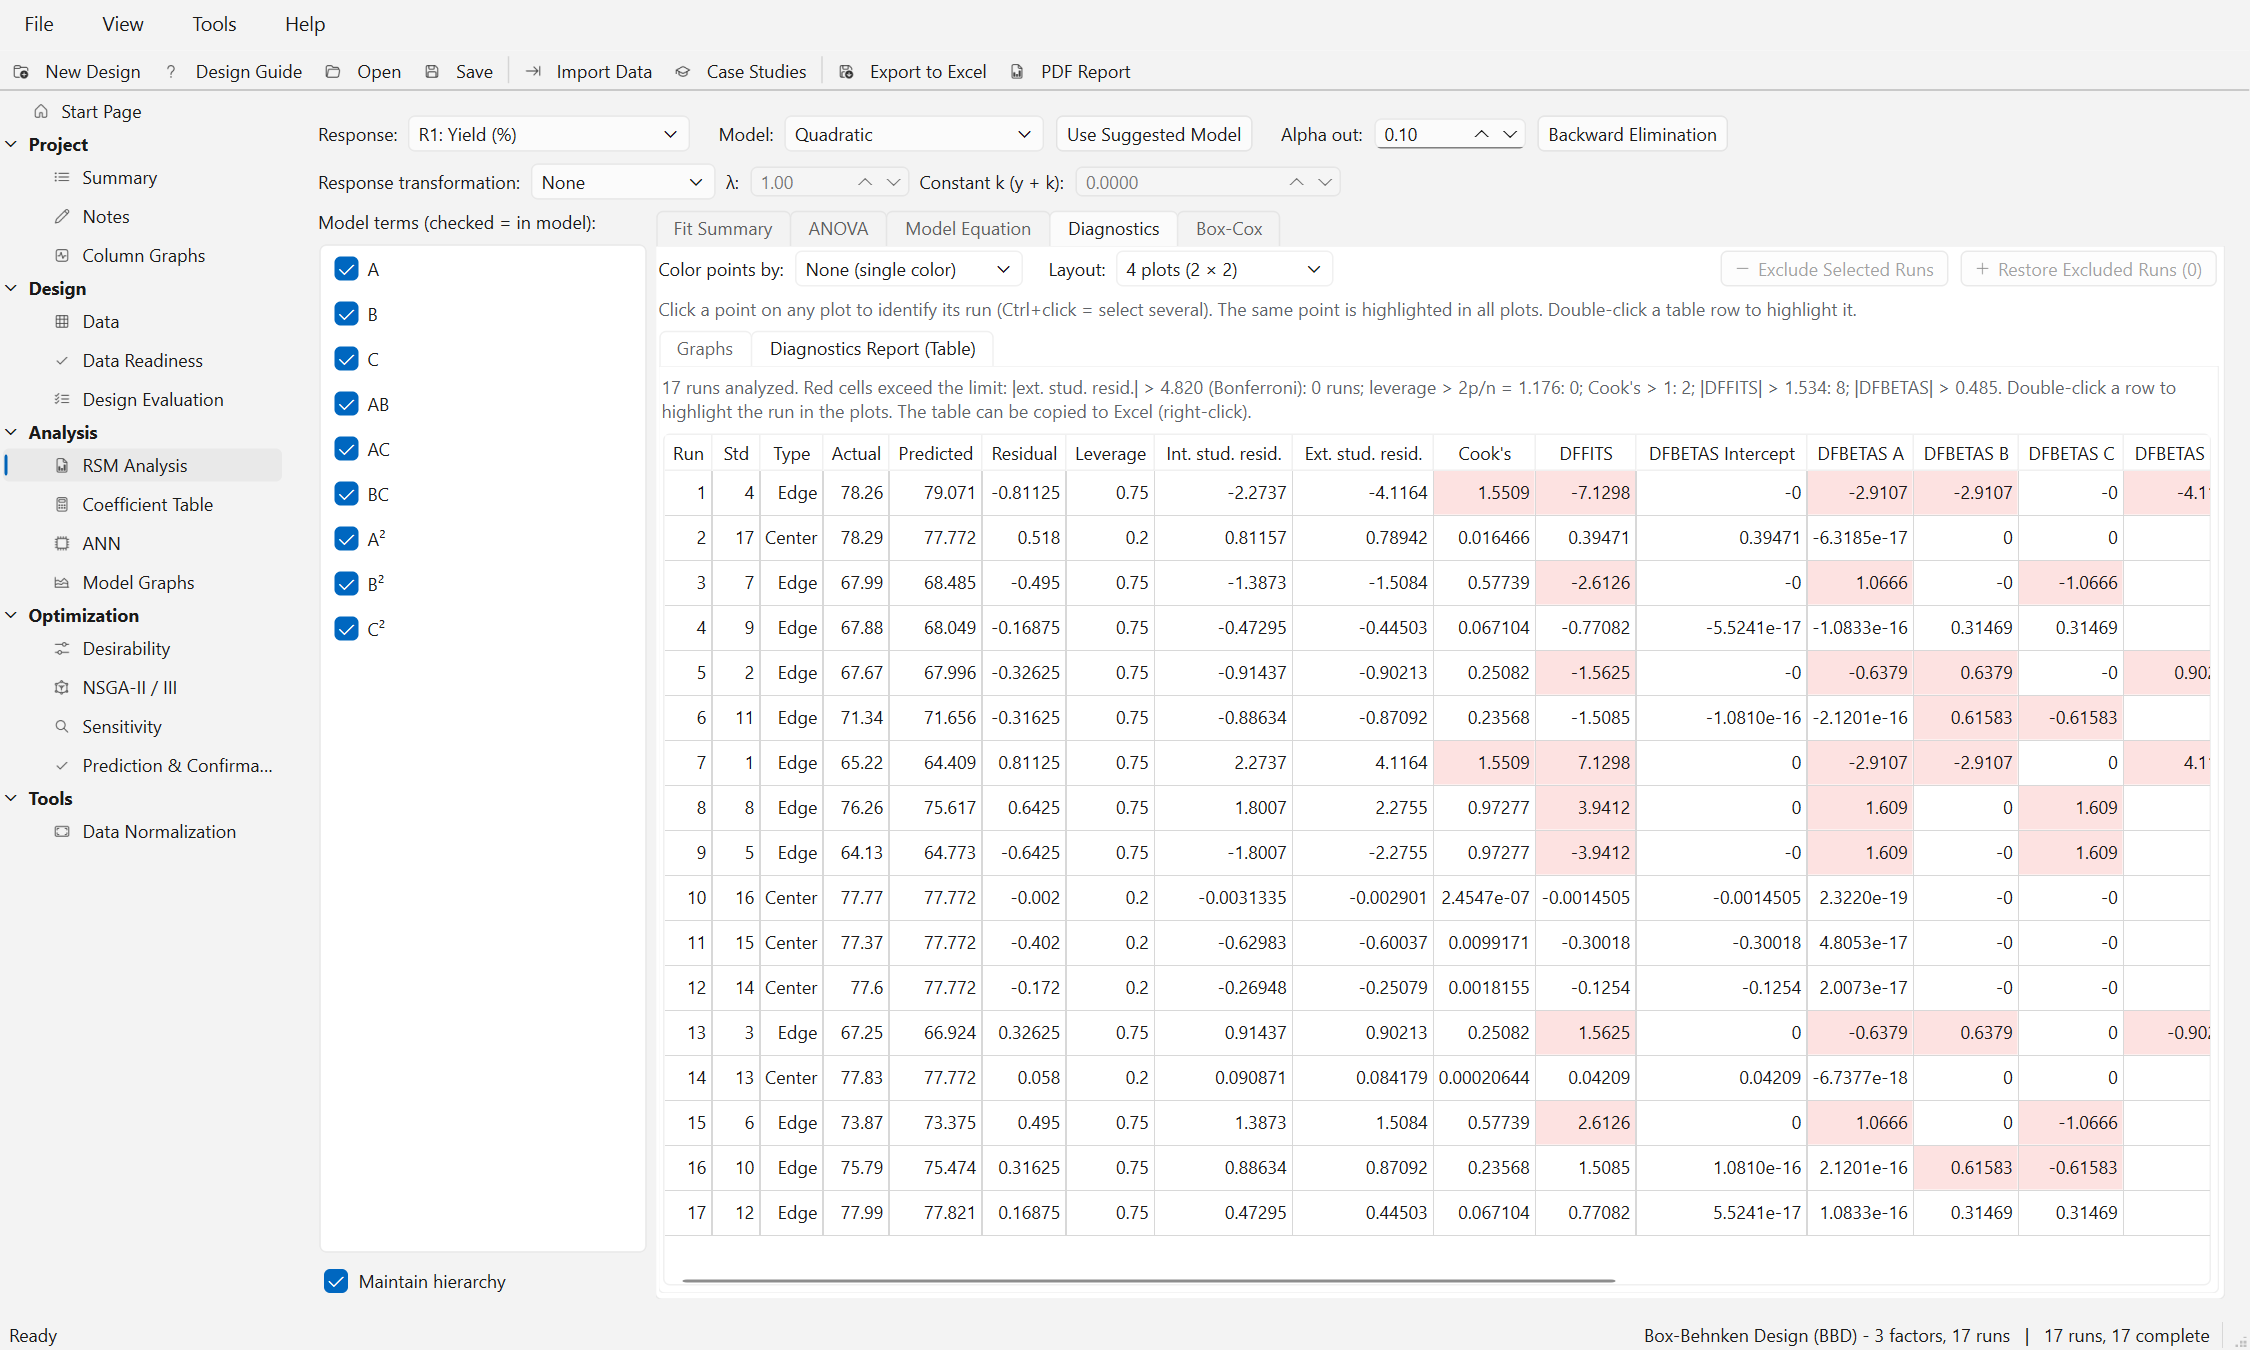
\includegraphics[width=\linewidth]{rsm_diagnostics_table.png}
\caption{Diagnostics Report (Table) for Yield (Box-Behnken case, no transformation) with the limits in the
header line (Cook's $>$ 1: 2 runs; $|$DFFITS$|$ $>$ 1.534: 8 runs) and red cells for values beyond them; all 17
runs are visible.}
\label{fig:ch05-diagtable}
\end{figure}

\subsection*{Excluding runs}
\ui{Exclude Selected Runs} (tooltip: ``Remove the runs from the analysis (the data is not deleted and can
be restored).'') marks the selected runs as excluded. Their response values are treated as missing by
every model, graph and optimization; the data stay on the \ui{Data} page and are marked in the Excel export
and the PDF report. \ui{Restore Excluded Runs (N)} brings all of them back. Exclude a run only when there is
a reason outside the statistics (a recorded mistake, a failed measurement), and always compare the model
before and after.

\subsection*{Example: Box-Behnken extraction, Yield}
Figures~\ref{fig:ch05-diag} and \ref{fig:ch05-diagtable} show the quadratic model. The normal plot is
close to a straight line and the Shapiro-Wilk $p$ is 0.904. The Bonferroni limit is
$t_{1-0.05/34,\,6}=4.820$; the largest $|t_i|$ is 4.12, so no run is an outlier. Leverage is 0.75 for the
edge runs and 0.20 for the center runs, all below $2p/n=1.176$. Runs 1 and 7 have Cook's distance 1.55
($>1$) and 8 runs exceed the DFFITS limit 1.534. Runs 1 and 7 are the AB-edge points (Temperature 60 °C,
Time 30 min) and (80 °C, 90 min). Excluding them shows why such a decision needs care: R² rises to 0.9973
and Predicted R² to 0.9675, but with only two AB-edge points left, AB and C² can no longer be separated and
C² is removed as aliased. The two runs carry the information about the AB interaction; they are influential
because the design has few runs, not because they are wrong. The Durbin-Watson statistic of this model is
1.98.

\section{Effects of two-level factorials}\label{sec:ch05-effects}

\subsection*{Purpose}
For unreplicated two-level designs there is no error estimate for a full model. The \ui{Effects (Factorial)}
sub-tab separates active effects from noise graphically and with Lenth's method \citep{lenth1989}.

\subsection*{When the sub-tab is shown}
The sub-tab appears for full factorial, fractional factorial and Plackett-Burman designs without categoric
factors and without split-plot structure. All numeric factor settings must be $-1$, 0 or $+1$ in coded
units (center points are allowed); otherwise the plot area shows ``Effect plots are only for 2-level
factorial designs.''

\subsection*{How to use}
\begin{enumerate}
  \item Choose the plot in \ui{Graph:} (\ui{Half-Normal}, \ui{Normal} or \ui{Pareto}).
  \item Click \ui{Select Automatically (Lenth ME Limit)}: every effect with $|\text{effect}|\ge\text{ME}$ is
        put in the model, together with its parent terms. If no effect qualifies: ``No effect exceeds the ME
        limit.''
  \item Click a point on the half-normal or normal plot (within 12 pixels) to add that term to the model or
        remove it; \ui{Maintain hierarchy} applies. Pareto bars are not clickable.
  \item \ui{Clear Selection} leaves the intercept-only model.
  \item Check the resulting model on the ANOVA sub-tab: the unselected effects now form the residual.
\end{enumerate}

\subsection*{Theory as implemented}
The program fits the model with all interactions of the factors (aliased columns removed) and computes each
effect as twice the coded coefficient, $c_j=2\hat\beta_j$, which is the difference between the mean response
at the high and at the low level. For Plackett-Burman designs only main effects are estimated, because
their two-factor interactions are partially aliased with the main effects; the unassigned columns then
provide residual degrees of freedom. With $m$ effects, Lenth's method is
\begin{align}
  s_0&=1.5\,\operatorname{median}_j|c_j|, \qquad
  \text{PSE}=1.5\,\operatorname{median}\{|c_j|:|c_j|<2.5\,s_0\}, \label{eq:ch05-pse}\\
  \text{ME}&=t_{0.975,\,d}\,\text{PSE},\qquad \text{SME}=t_{\gamma,\,d}\,\text{PSE},\qquad
  d=\frac m3,\quad \gamma=\frac{1+0.95^{1/m}}{2}. \label{eq:ch05-me}
\end{align}
PSE (pseudo standard error) is a robust estimate of the standard error of an effect based on the small
effects. ME is a margin of error for one effect at the 5\% level; SME is a simultaneous margin that controls
the error rate over all $m$ effects. An effect beyond SME is clearly active; one between ME and SME is
possibly active \citep{lenth1989}.

\paragraph{Plots.}
\begin{itemize}
  \item \emph{Half-Normal}: $|c_j|$ (axis \ui{|Effect|}) against the half-normal quantile of $(i-0.5)/m$
        (axis \ui{Half-normal (\%)}). Blue points are ``Error'', orange points ``Selected (model)''. Selected
        terms and terms beyond ME are labeled. A red dashed line through the origin follows the unselected
        effects (slope = median of $|c|/q$). Vertical lines show ``ME (Lenth)'' (dashed) and ``SME (Lenth)''
        (dotted).
  \item \emph{Normal}: signed effects (axis \ui{Effect}) against normal quantiles, with ME and SME on both
        sides.
  \item \emph{Pareto}: bars of $|t|$ sorted from large to small (orange = selected). Without residual df,
        $t=|c_j|/\text{PSE}$, the title adds ``(based on Lenth's PSE)'' and the lines are ME and SME in
        $t$ units ($t_{0.975,d}$ and $t_{\gamma,d}$). With residual df (replicates, center points or
        Plackett-Burman spare columns) $t=|c_j|/\text{se}(c_j)$ with lines ``t limit'' $t_{0.975,\nu}$
        and ``Bonferroni'' $t_{1-0.05/(2m),\nu}$.
\end{itemize}
The text below the plot gives ``PSE Lenth = \dots, ME = \dots, SME = \dots{} (Lenth 1989)'' and lists
aliased terms, if any.

\begin{figure}[htbp]\centering
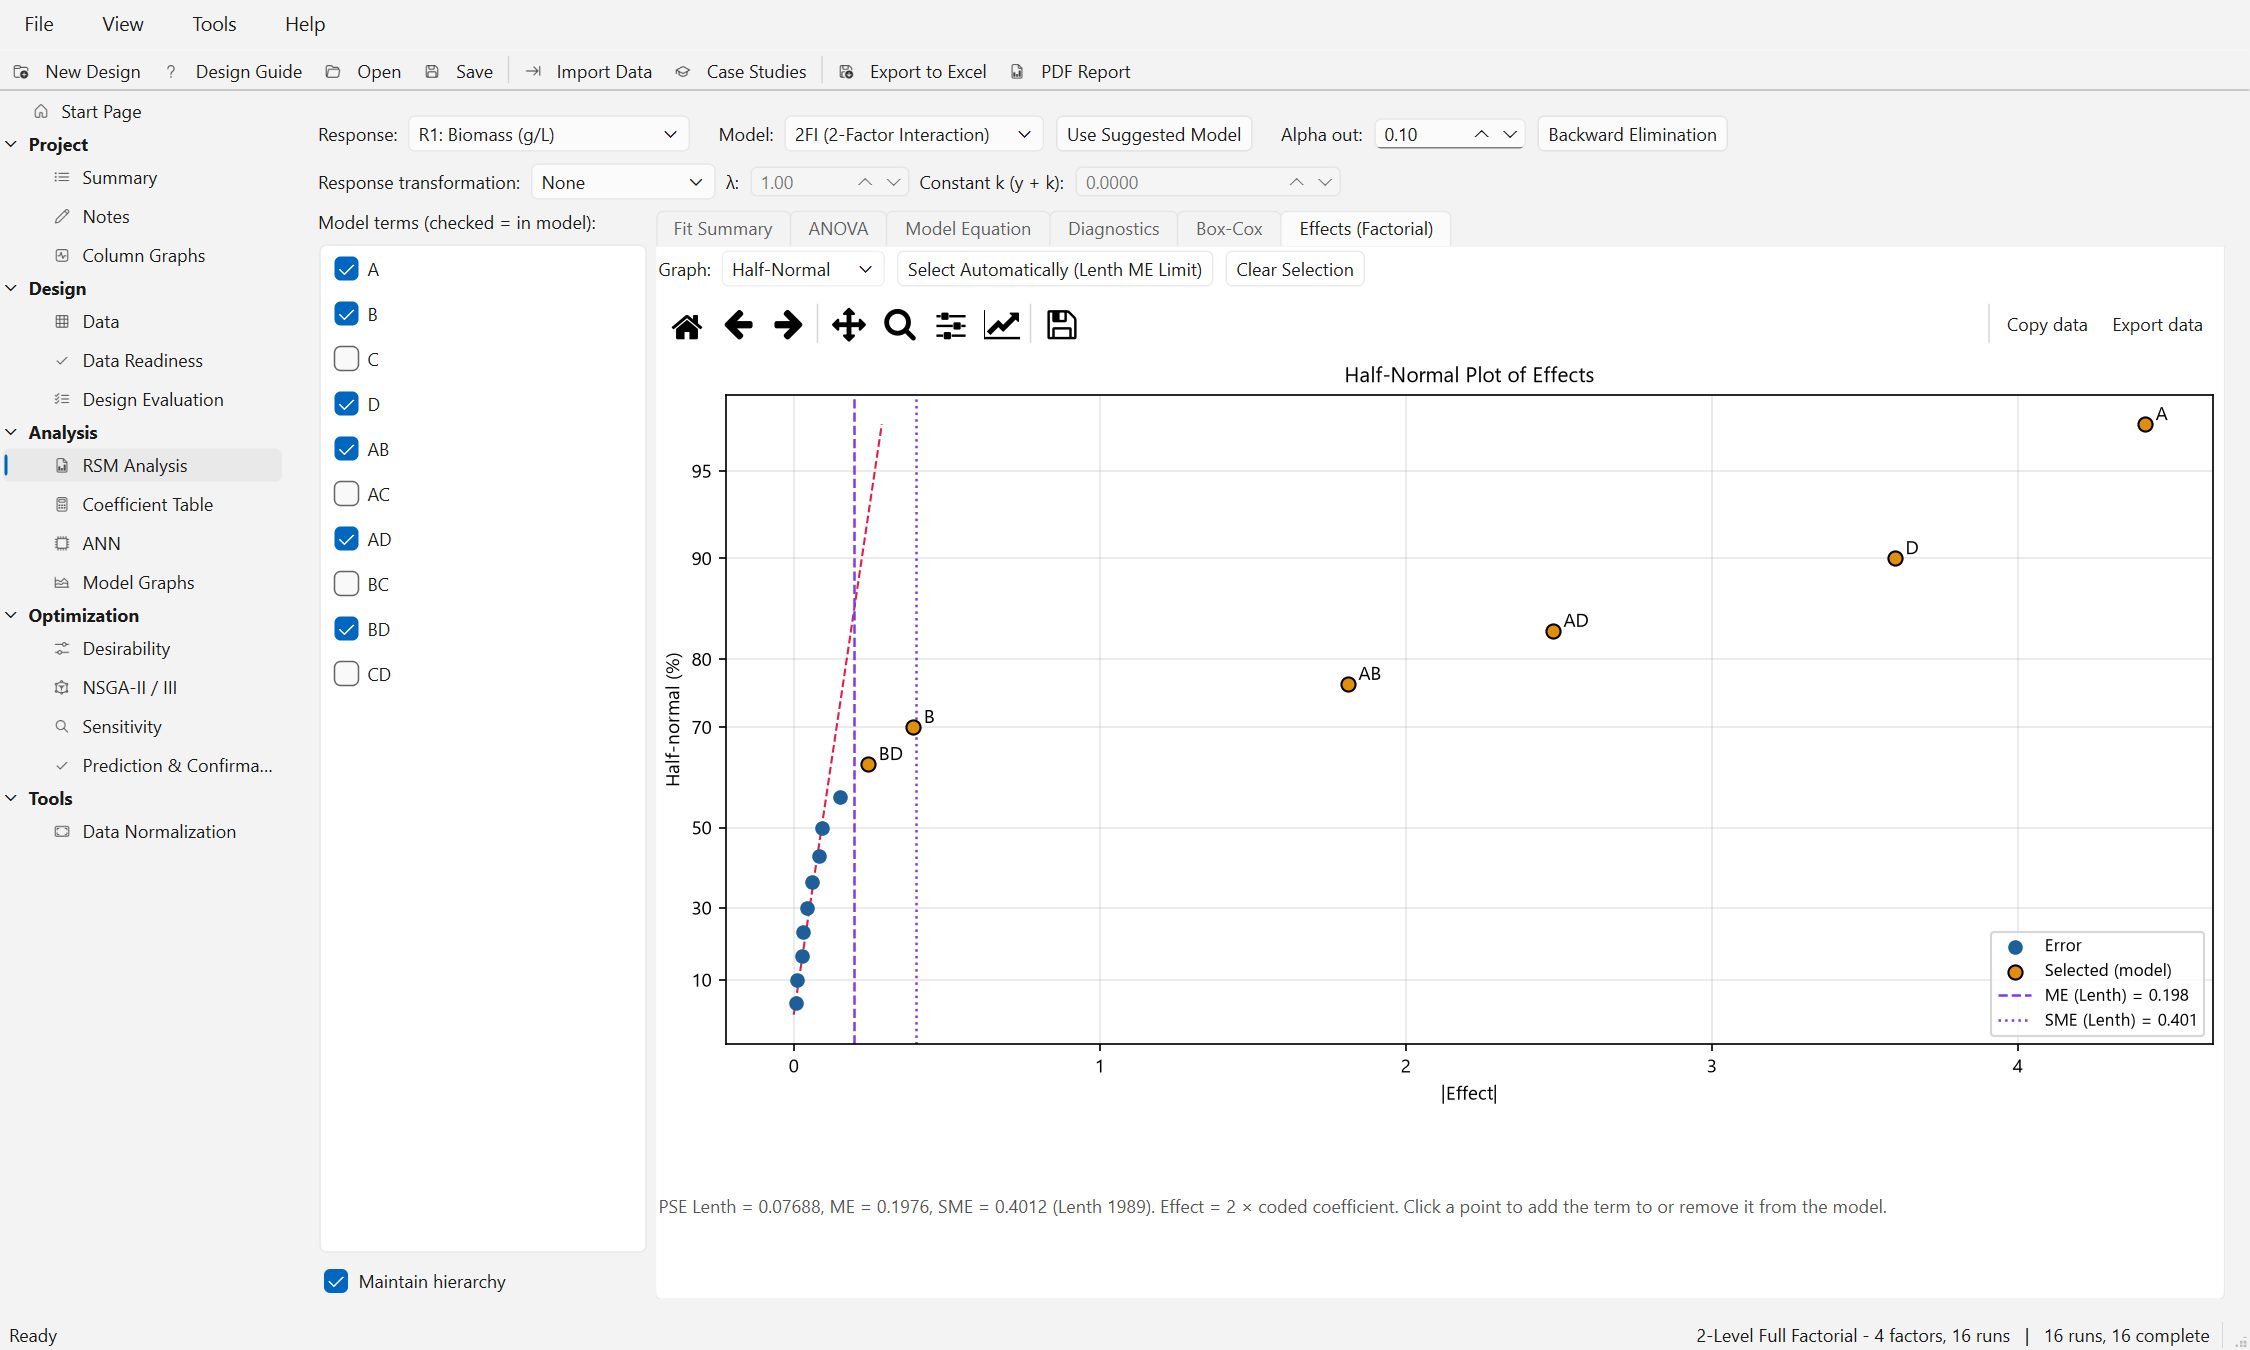
\includegraphics[width=\linewidth]{effects_halfnormal.png}
\caption{Half-normal plot of effects for Biomass (2$^4$ fermentation screening) after
\ui{Select Automatically (Lenth ME Limit)}, with the ME and SME lines.}
\label{fig:ch05-halfnormal}
\end{figure}

\begin{figure}[htbp]\centering
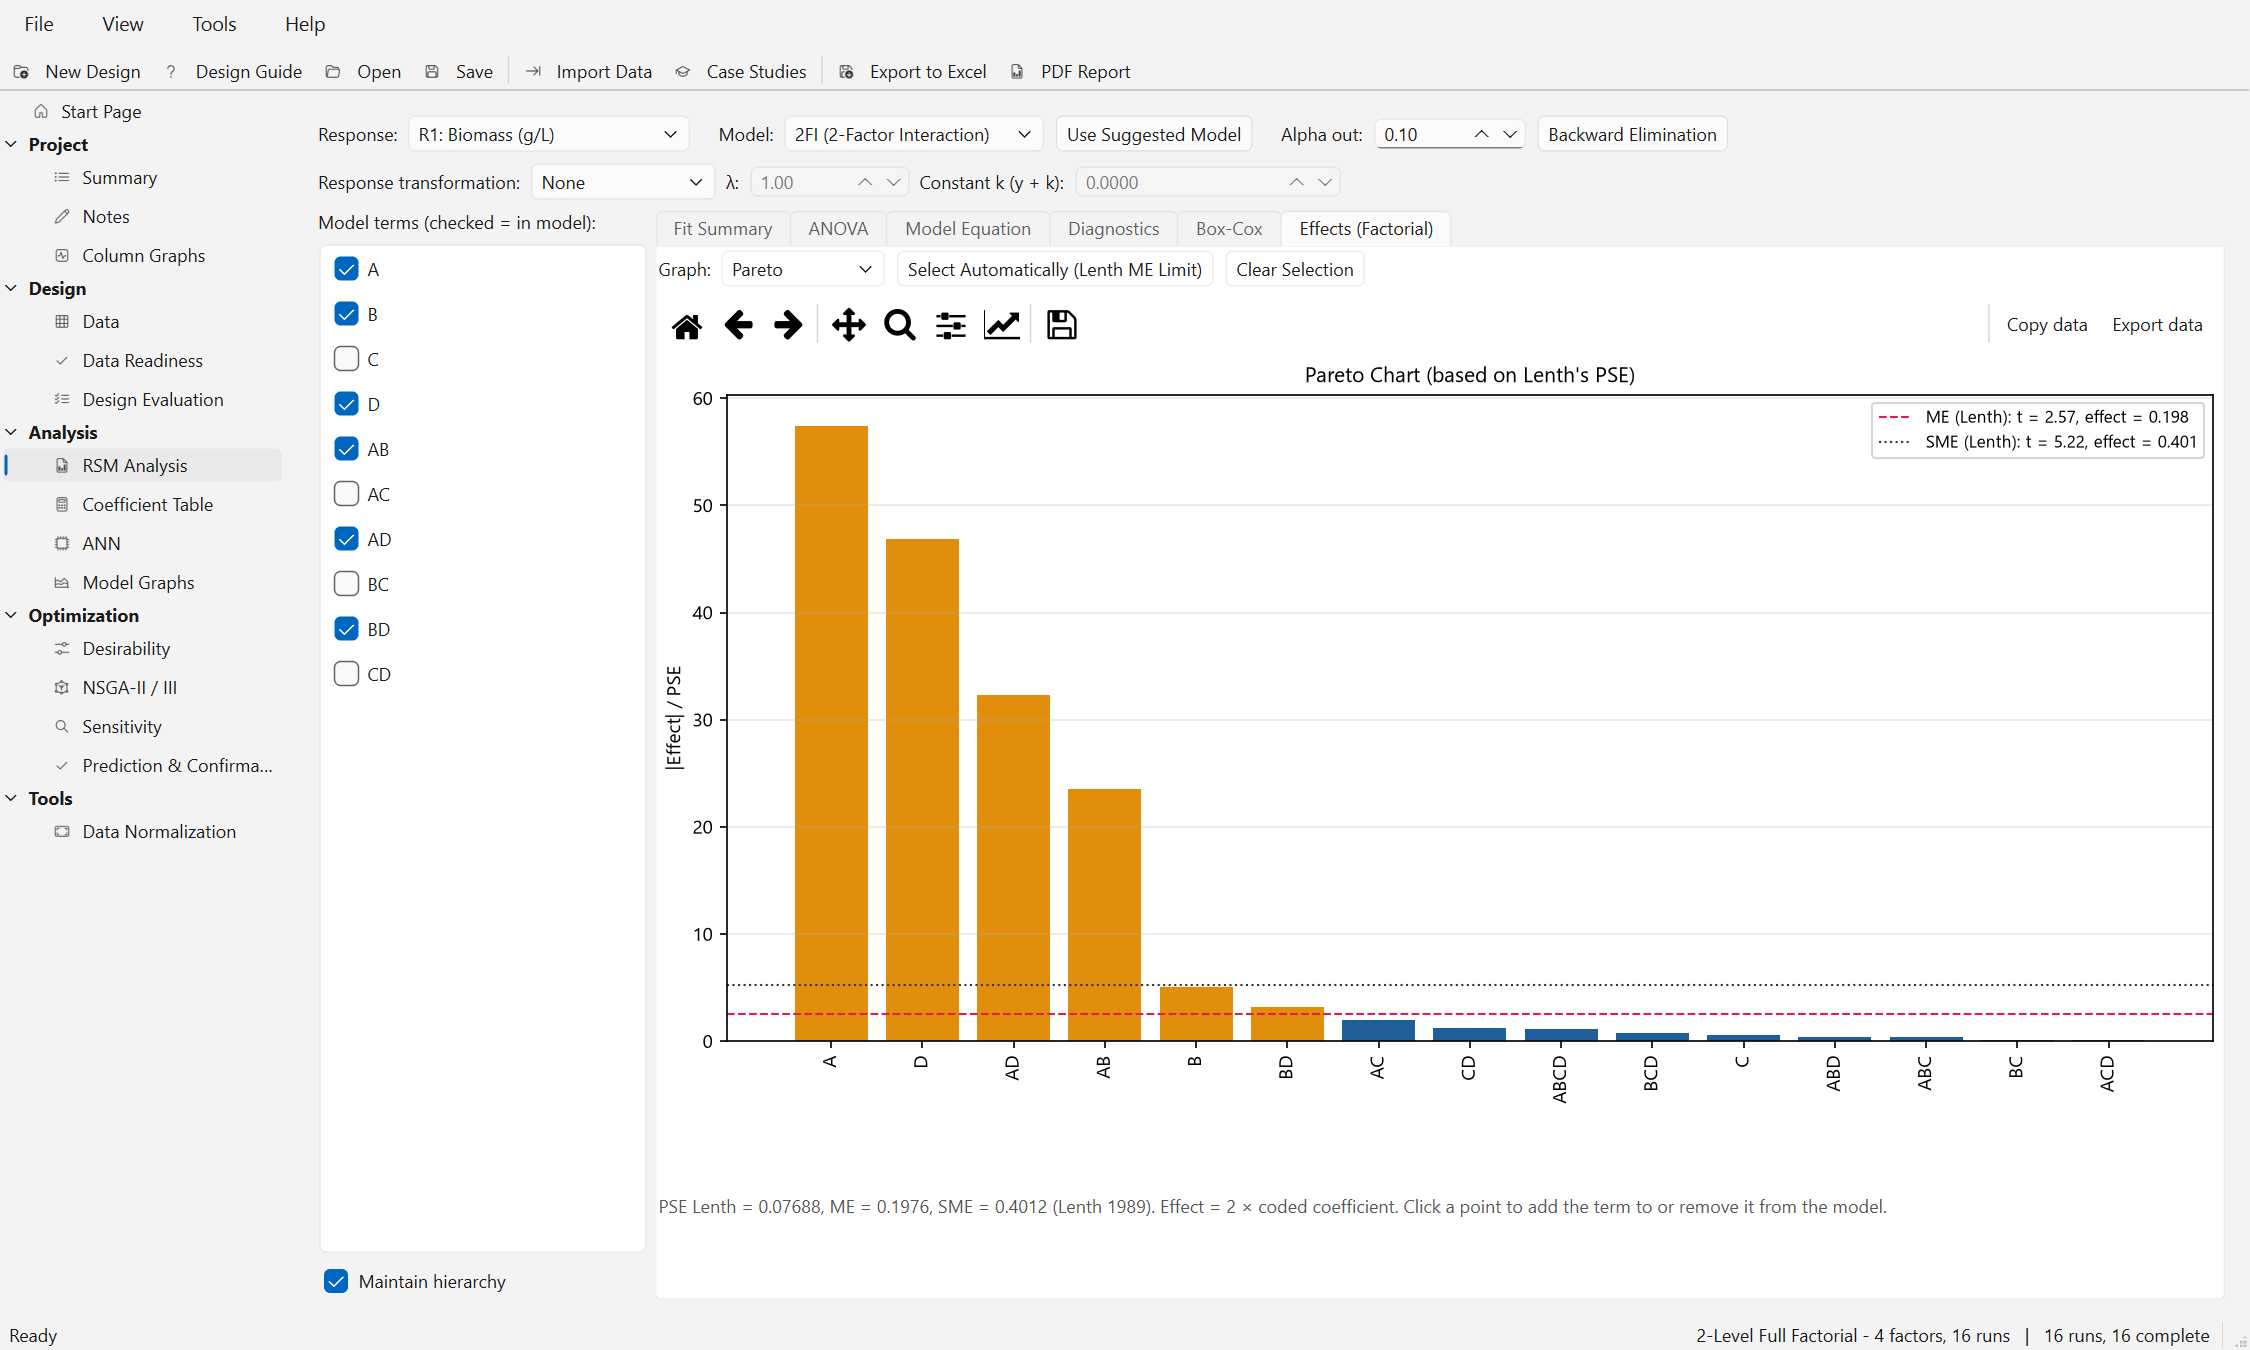
\includegraphics[width=\linewidth]{effects_pareto.png}
\caption{Pareto chart of the same effects, $|$effect$|$/PSE with the ME and SME limits.}
\label{fig:ch05-pareto}
\end{figure}

\subsection*{Example: Fermentation Screening (2$^4$ factorial)}
The 16 runs give 15 effects: A 4.416, D 3.599, AD 2.481, AB $-1.811$, B 0.391, BD $-0.244$; all others are
at most 0.151 in absolute value. Lenth's method gives PSE = 0.07688, ME = 0.1976 and SME = 0.4012
($d=5$, $t_{0.975,5}=2.571$, $t_{\gamma,5}=5.219$). \ui{Select Automatically (Lenth ME Limit)} selects A, B,
D, AB, AD and BD (Figure~\ref{fig:ch05-halfnormal}). A, D, AB and AD exceed SME; B and BD lie between ME and
SME, so they are only possibly active. The ANOVA of the selected model (Figure~\ref{fig:ch05-effanova}) has
9 residual df: Model $F=1385$ ($p<0.0001$), B $p=0.0004$, BD $p=0.0076$, R² 0.99892, Adjusted R² 0.9982,
Predicted R² 0.99658, Adeq Precision 107.0. The Fit Summary of this case (default 2FI) gives Linear
$p=0.0015$, 2FI $p<0.0001$ (Suggested) and 3FI $p=0.9165$; lack of fit cannot be tested because there are
no replicates.

\begin{figure}[htbp]\centering
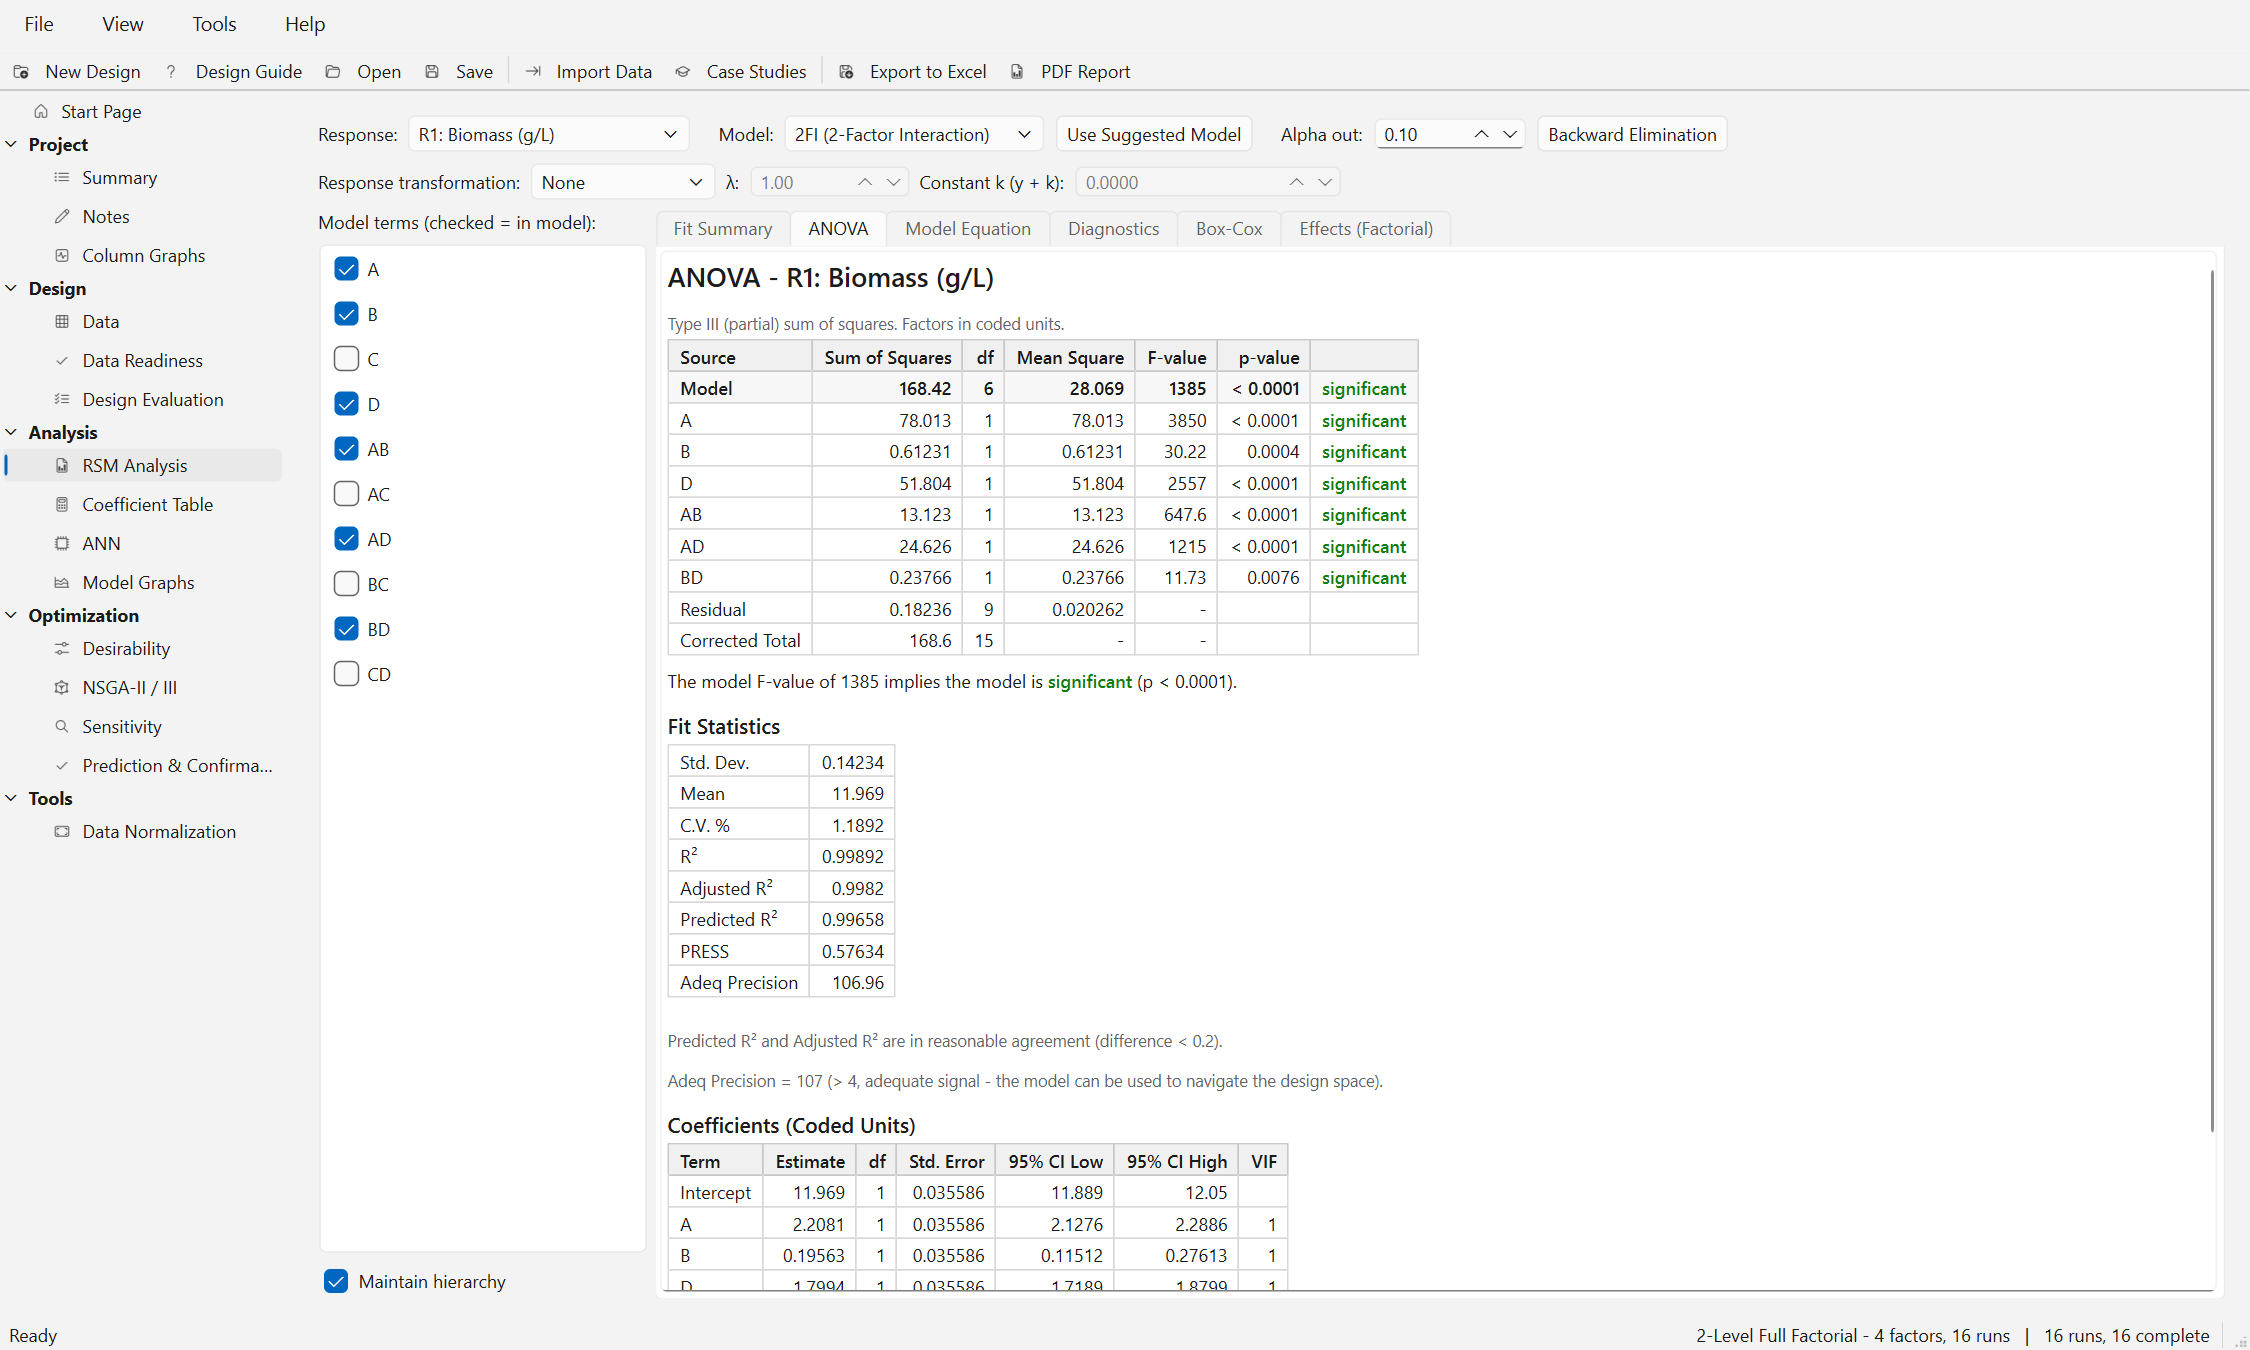
\includegraphics[width=\linewidth]{effects_anova.png}
\caption{ANOVA of the factorial model selected on the effects plot.}
\label{fig:ch05-effanova}
\end{figure}

\section{Logistic and Poisson regression (GLM)}\label{sec:ch05-glm}

\subsection*{Purpose}
Counts and numbers of successes do not have constant variance and cannot be negative or exceed the number
of trials. For such responses REGEN fits a generalized linear model (GLM) \citep{mccullagh1989} instead of
least squares.

\subsection*{How to use}
\begin{enumerate}
  \item On the \ui{Data} page click \ui{Factor \& Response Info\dots} and set \ui{Type} of the response to
        \ui{Binomial (successes out of n)} (enter \ui{Trials per run}) or \ui{Poisson (counts)}. Enter the
        data as the number of successes per run, or as counts.
  \item On the RSM Analysis page the ANOVA sub-tab is now called \ui{GLM (Logistic/Poisson)} and the
        transformation box is disabled.
  \item Choose the model with the Fit Summary (likelihood-ratio version), remove terms with
        \ui{Backward Elimination}, and check the diagnostics.
\end{enumerate}

\subsection*{Theory as implemented}
\paragraph{Model.} For run $i$ with $m$ trials and model row $x_i$:
\begin{align}
  \text{binomial:}\quad & y_i\sim\text{Bin}(m,\pi_i),\quad \ln\frac{\pi_i}{1-\pi_i}=x_i'\beta
  \quad\text{(logit link)}, \label{eq:ch05-logit}\\
  \text{Poisson:}\quad & y_i\sim\text{Pois}(\mu_i),\quad \ln\mu_i=x_i'\beta\quad\text{(log link)}.
  \label{eq:ch05-poisson}
\end{align}

\paragraph{Estimation (IRLS).} Starting from $\eta=\operatorname{logit}\bar p$,
$\bar p=(\sum y+0.5)/(mn+1)$ (binomial) or $\eta=\ln\max(y,0.5)$ (Poisson), the program iterates
\begin{equation}
  w_i=m\pi_i(1-\pi_i)\ \text{or}\ \mu_i,\qquad z_i=\eta_i+\frac{y_i-\mu_i}{w_i},\qquad
  \beta\leftarrow(X'WX)^{-1}X'Wz,
  \label{eq:ch05-irls}
\end{equation}
with $\mu_i=m\pi_i$ for the binomial, until $\max|\Delta\beta|<10^{-10}(1+\max|\beta|)$ or 100 iterations.
The covariance of $\hat\beta$ is $(X'WX)^{-1}$, so the Wald statistic is $z=\hat\beta_j/\text{se}_j$ and the
95\% CI uses 1.96.

\paragraph{Deviance and tests.} The deviance compares the model with the saturated model:
\begin{align}
  D_{\text{bin}}&=2\sum_i\Big[y_i\ln\frac{y_i}{\hat\mu_i}+(m-y_i)\ln\frac{m-y_i}{m-\hat\mu_i}\Big],
  \qquad D_{\text{Pois}}=2\sum_i\Big[y_i\ln\frac{y_i}{\hat\mu_i}-(y_i-\hat\mu_i)\Big]. \label{eq:ch05-dev}
\end{align}
The model is tested with $\chi^2=D_0-D$ on $p-p_0$ df, where the null model contains the intercept (and
blocks). Each term is tested by refitting without its columns: $\chi^2_t=D_{(-t)}-D$ on $df_t$ df (a
Type III likelihood-ratio test). The sequential test of the Fit Summary is $D_{\text{ref}}-D$ on
$p-p_{\text{ref}}$ df.

\paragraph{Goodness of fit and statistics.}
\begin{itemize}
  \item Deviance and Pearson $\chi^2=\sum(y_i-\hat\mu_i)^2/V(\hat\mu_i)$, with $V=\hat\mu(1-\hat\mu/m)$
        (binomial) or $V=\hat\mu$ (Poisson), are compared with $\chi^2_{n-p}$. Dispersion = Pearson
        $\chi^2/(n-p)$; values well above 1 mean overdispersion (the standard errors are then too small).
  \item Hosmer-Lemeshow test (binomial) \citep{hosmer1980}: the runs are sorted by $\hat\pi$ and split into
        $g=\min(10,\max(2,\lfloor n/2\rfloor))$ groups;
        $\chi^2_{HL}=\sum_g(O_g-E_g)^2/\big(N_g\bar\pi_g(1-\bar\pi_g)\big)$, with $O_g$, $E_g$ the observed
        and expected successes and $N_g$ the trials in group $g$, on $\max(g-2,1)$ df.
  \item AIC $=-2\ell+2p$, BIC $=-2\ell+p\ln n$, McFadden pseudo R² $=1-\ell/\ell_0$ and Adj.\ McFadden
        $=1-(\ell-p)/\ell_0$, where $\ell$ and $\ell_0$ are the log-likelihoods of the model and the null
        model.
  \item Tjur R² (binomial) \citep{tjur2009}: mean fitted probability of the successes minus that of the
        failures, $\sum y_i\hat\pi_i/\sum y_i-\sum(m-y_i)\hat\pi_i/\sum(m-y_i)$.
\end{itemize}

\paragraph{Warnings.} The program warns when IRLS does not converge within 100 iterations, and when fitted
probabilities are numerically 0 or 1 (binomial) or fitted means numerically 0 (Poisson). The latter
indicates complete or quasi-complete separation: some coefficients tend to infinity, and their standard
errors, $z$ tests and odds ratios are not reliable. Very large coefficients ($|\hat\beta|>10$) are then
listed. The warnings appear at the top of the GLM sub-tab, and the red error label says ``The GLM fit has
warnings - see the GLM (Logistic/Poisson) tab.'' Remove terms or add runs where the response changes.

\paragraph{Diagnostics and predictions.} Residuals are deviance residuals
$\text{sign}(y_i-\hat\mu_i)\sqrt{d_i}$ standardized by $\sqrt{1-h_{ii}}$, with leverage from $W^{1/2}X$.
Cook's distance is $r_{P,i}^2h_{ii}/\big(p(1-h_{ii})^2\big)$ with the Pearson residual $r_{P,i}$; DFFITS uses
the standardized deviance residual; DFBETAS is not available. \ui{Predicted vs Actual} is on the response
scale: observed proportion against fitted probability, or observed count against fitted mean. Predictions,
graphs and optimization use $\hat\pi$ or $\hat\mu$; the 95\% CI is $g^{-1}(\hat\eta\pm1.96\,\text{se}_\eta)$.
No prediction interval is given.

\subsection*{Output}
The sub-tab (Figure~\ref{fig:ch05-glm}) shows the heading ``Logistic Regression - \dots'' or ``Poisson
Regression - \dots'', the note ``Link: logit. Trials per run = 50. Terms are tested with the likelihood ratio
($\chi^2$).'', the test table (\ui{Source}, \ui{$\chi^2$}, \ui{df}, \ui{p-value}), \ui{Fit Statistics},
\ui{Goodness-of-Fit Tests} and the coefficient table on the logit or log scale with \ui{z}, \ui{p-value},
confidence limits and \ui{Odds ratio} or \ui{Rate ratio} $=e^{\hat\beta}$. The note under the GOF table
reads: ``A goodness-of-fit p-value $>$ 0.05 means there is no evidence of lack of fit. Dispersion well
above 1 indicates overdispersion.''

\begin{figure}[htbp]\centering
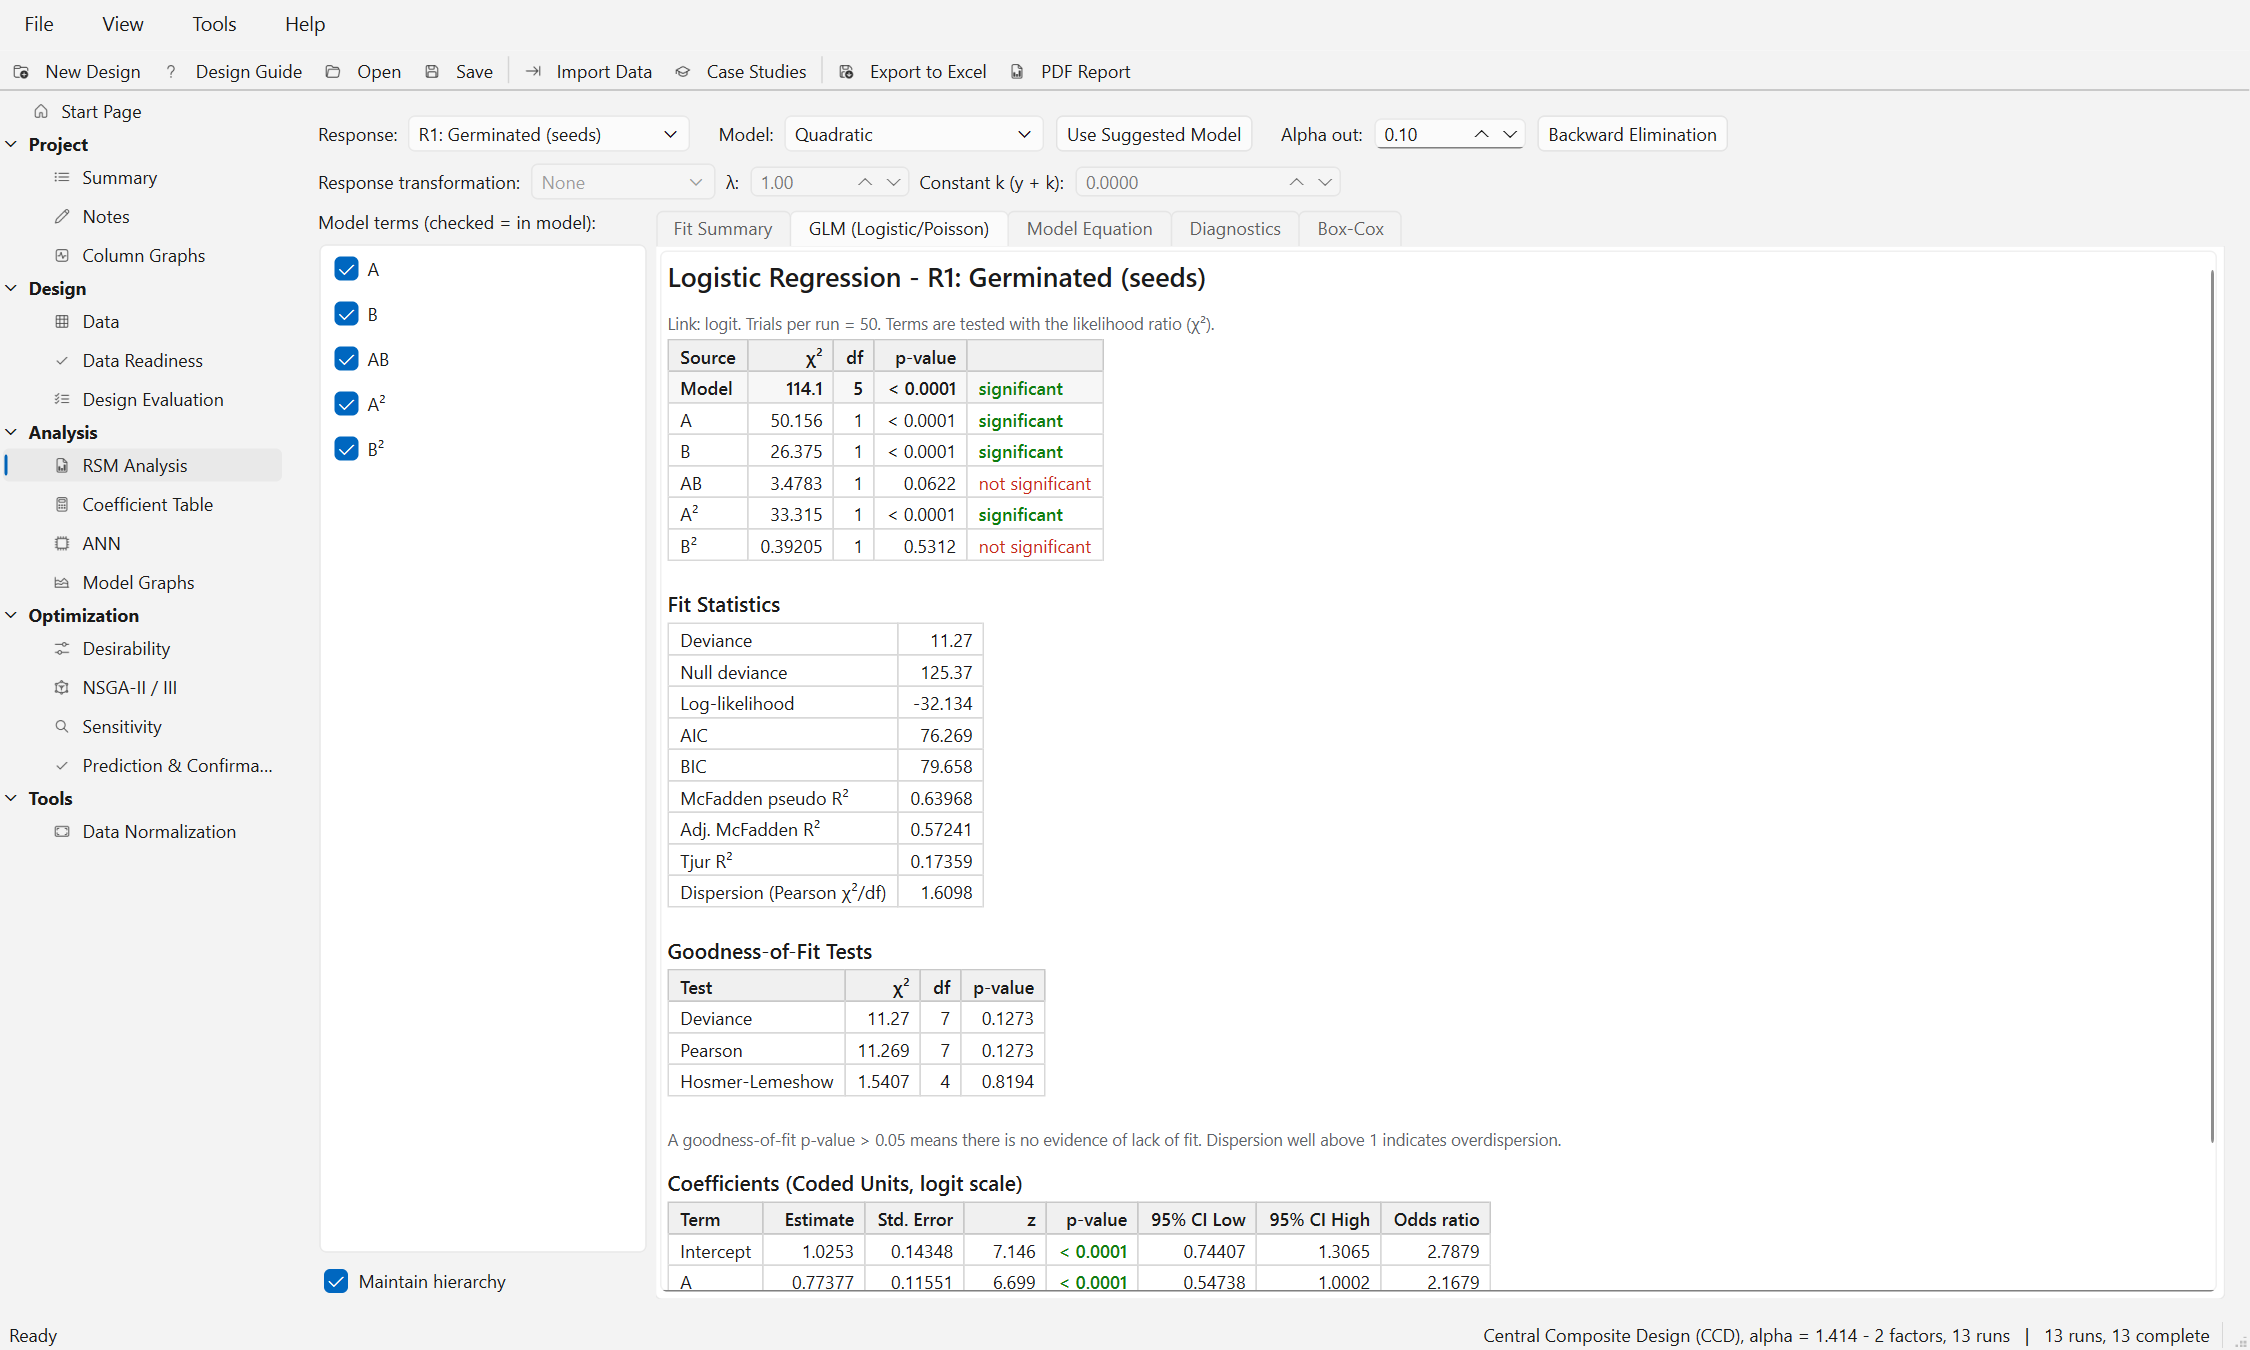
\includegraphics[width=\linewidth]{glm_logistic.png}
\caption{GLM (Logistic/Poisson) sub-tab for the seed germination case: likelihood-ratio tests, fit
statistics, goodness-of-fit tests and coefficients with odds ratios.}
\label{fig:ch05-glm}
\end{figure}

\subsection*{Example: Seed Germination (logistic regression)}
The case is a CCD in Temperature (20--35 °C) and Humidity (60--90\%) with 13 runs of 50 seeds. The Fit
Summary gives Linear ($p<0.0001$, deviance 46.94, AIC 105.94), 2FI ($p=0.1257$), Quadratic ($p<0.0001$,
deviance 11.27, AIC 76.27, McFadden 0.640, Suggested) and Cubic ($p=0.384$, Aliased). For the quadratic
model the likelihood-ratio tests are: Model $\chi^2=114.1$ on 5 df, A 50.16, B 26.38, AB 3.48 ($p=0.0622$),
A² 33.32 and B² 0.39 ($p=0.5312$). Deviance 11.27 on 7 df ($p=0.1273$), Pearson $p=0.1273$,
Hosmer-Lemeshow $\chi^2=1.54$ on 4 df ($p=0.8194$): no lack of fit. Dispersion is 1.61, slightly above 1.
McFadden R² is 0.640 (adjusted 0.572), Tjur R² 0.174. Tjur's R² is small because it measures how well single
seeds are separated, and the germination probability only ranges over moderate values. The odds ratios
are A 2.168, B 1.777, AB 0.742 and A² 0.495. Because the model contains AB and A², an odds ratio of a
single coefficient is not the change in odds for a change of the factor; use the model graphs to see the
combined effect. IRLS converged in 5 iterations without warnings. At the center the
predicted germination probability is 0.736 (95\% CI 0.678 to 0.787).

\section{Split-plot analysis with REML}\label{sec:ch05-reml}

\subsection*{Purpose}
In a split-plot experiment the hard-to-change (HTC) factors are set once per whole plot, and the
easy-to-change factors vary within it. Runs in the same whole plot share a random whole-plot error, so
ordinary least squares gives wrong tests: HTC effects look more significant than they are. REGEN fits a
linear mixed model by restricted maximum likelihood (REML) \citep{patterson1971,goos2011}.

\subsection*{How to use}
The analysis is used automatically for projects with whole plots (created with the split-plot option in
\ui{New Design}, with the hard-to-change factor letters). The ANOVA sub-tab is called
\ui{Split-Plot (REML)}, \ui{Use Suggested Model} is hidden, the Fit Summary is not available and Box-Cox is
not offered. Transformations, term selection and backward elimination work as usual. There is no overall
model F test and no least-squares R², adjusted R² or predicted R² for this model (only the conditional R² of
the statistics table); judge it by the Wald F tests of its terms. The
\ui{Data Readiness} page therefore shows ``Model fit'' and ``Model significance'' as Info checks for split-plot
responses (Chapter~\ref{chap:4}).

\subsection*{Theory as implemented}
\paragraph{Model.}
\begin{equation}
  y=X\beta+Zu+\varepsilon,\qquad u_g\sim N(0,\sigma^2_{wp}),\quad \varepsilon_i\sim N(0,\sigma^2),
  \label{eq:ch05-mixed}
\end{equation}
where $Z$ assigns runs to whole plots. With $\gamma=\sigma^2_{wp}/\sigma^2$ the covariance is
$\sigma^2V_0$, $V_0=I+\gamma ZZ'$. Each whole-plot block of $V_0^{-1}$ is
$I-\frac{\gamma}{1+\gamma m_g}J$ ($m_g$ runs in plot $g$, $J$ a matrix of ones) and
$\ln|V_0|=\sum_g\ln(1+\gamma m_g)$.

\paragraph{REML.} For a given $\gamma$, the generalized least-squares estimate and the profile REML criterion
are
\begin{align}
  \hat\beta&=(X'V_0^{-1}X)^{-1}X'V_0^{-1}y,\qquad
  \hat\sigma^2=\frac{r'V_0^{-1}r}{n-p},\quad r=y-X\hat\beta, \label{eq:ch05-gls}\\
  -2\ell_R(\gamma)&=(n-p)\ln\hat\sigma^2+\ln|V_0|+\ln|X'V_0^{-1}X| \quad(\text{constants omitted}).
  \label{eq:ch05-reml}
\end{align}
The criterion is minimized over $\ln\gamma\in[-12,9]$. If the value at $\ln\gamma=-30$ is not worse, the
whole-plot variance is set to 0 (boundary). Then $\hat\sigma^2_{wp}=\gamma\hat\sigma^2$ and
$\text{Cov}(\hat\beta)=\hat\sigma^2(X'V_0^{-1}X)^{-1}$.

\paragraph{Wald F tests and denominator df.} Each term $t$ with $q_t$ columns is tested with
$F=\hat\beta_t'C_t^{-1}\hat\beta_t/q_t$, where $C_t$ is its block of $\text{Cov}(\hat\beta)$. The denominator
df follow the containment rule:
\begin{align}
  df_{wp}&=n_{wp}-(1+c_{wp}),\qquad df_{sp}=n-n_{wp}-(p-1-c_{wp}), \label{eq:ch05-dfcont}
\end{align}
with $n_{wp}$ whole plots and $c_{wp}$ the number of columns of whole-plot terms (terms made only of HTC
factors). The intercept and whole-plot terms are tested on $df_{wp}$, all other terms on $df_{sp}$. If a df
is 0, $n-p$ is used instead. The coefficient $t$ tests use the same df. The more refined Kenward-Roger
correction \citep{kenward1997} is not implemented; with few whole plots its df can be smaller.

\paragraph{Residuals.} The whole-plot effects are predicted by
$\hat u_g=\frac{\gamma}{1+\gamma m_g}\sum_{i\in g}r_i$ (BLUP). Diagnostics use the conditional residuals
$r_i-\hat u_{g(i)}$, studentized by $\sqrt{\hat\sigma^2(1-h_i/(1+\gamma))}$ with
$h_i=x_i'(X'V_0^{-1}X)^{-1}x_i$. Conditional R² $=1-\sum(r_i-\hat u_{g(i)})^2/\text{SST}$. Cook's distance and
DFFITS are not shown (neither in the plots nor in the table): their one-run deletion formulas assume
independent runs, which is not true within a whole plot, and a proper deletion diagnostic would have to
re-estimate the variance components. DFBETAS is not available either.

\paragraph{Predictions.} The confidence interval uses $\text{Cov}(\hat\beta)$; the prediction interval
for the mean of $m$ new runs adds $\hat\sigma^2_{wp}+\hat\sigma^2/m$. The POE graph uses
$\hat\sigma^2+\hat\sigma^2_{wp}$ as residual variance.

\subsection*{Output}
The sub-tab (Figure~\ref{fig:ch05-reml}) shows the heading ``Split-Plot Analysis (REML) - \dots'', the
note on the containment method, the test table (\ui{Term}, \ui{Type} = Whole plot or Subplot,
\ui{Numerator df}, \ui{Denominator df}, \ui{F-value}, \ui{p-value}), \ui{Variance Components} (\ui{Whole plot
(between groups)} and \ui{Subplot (residual)} with variance, standard deviation and \% of the total),
\ui{Statistics} (number of whole plots, df whole plot, df subplot, variance ratio $\gamma$, $-2$ REML
log-likelihood, conditional R², mean) and \ui{Coefficients (GLS)} with $t$ tests. If $df_{wp}\le0$ the
warning ``Whole-plot df = 0: hard-to-change factor effects cannot be tested properly. Add more whole plots
(replicates).'' is shown.

\begin{figure}[htbp]\centering
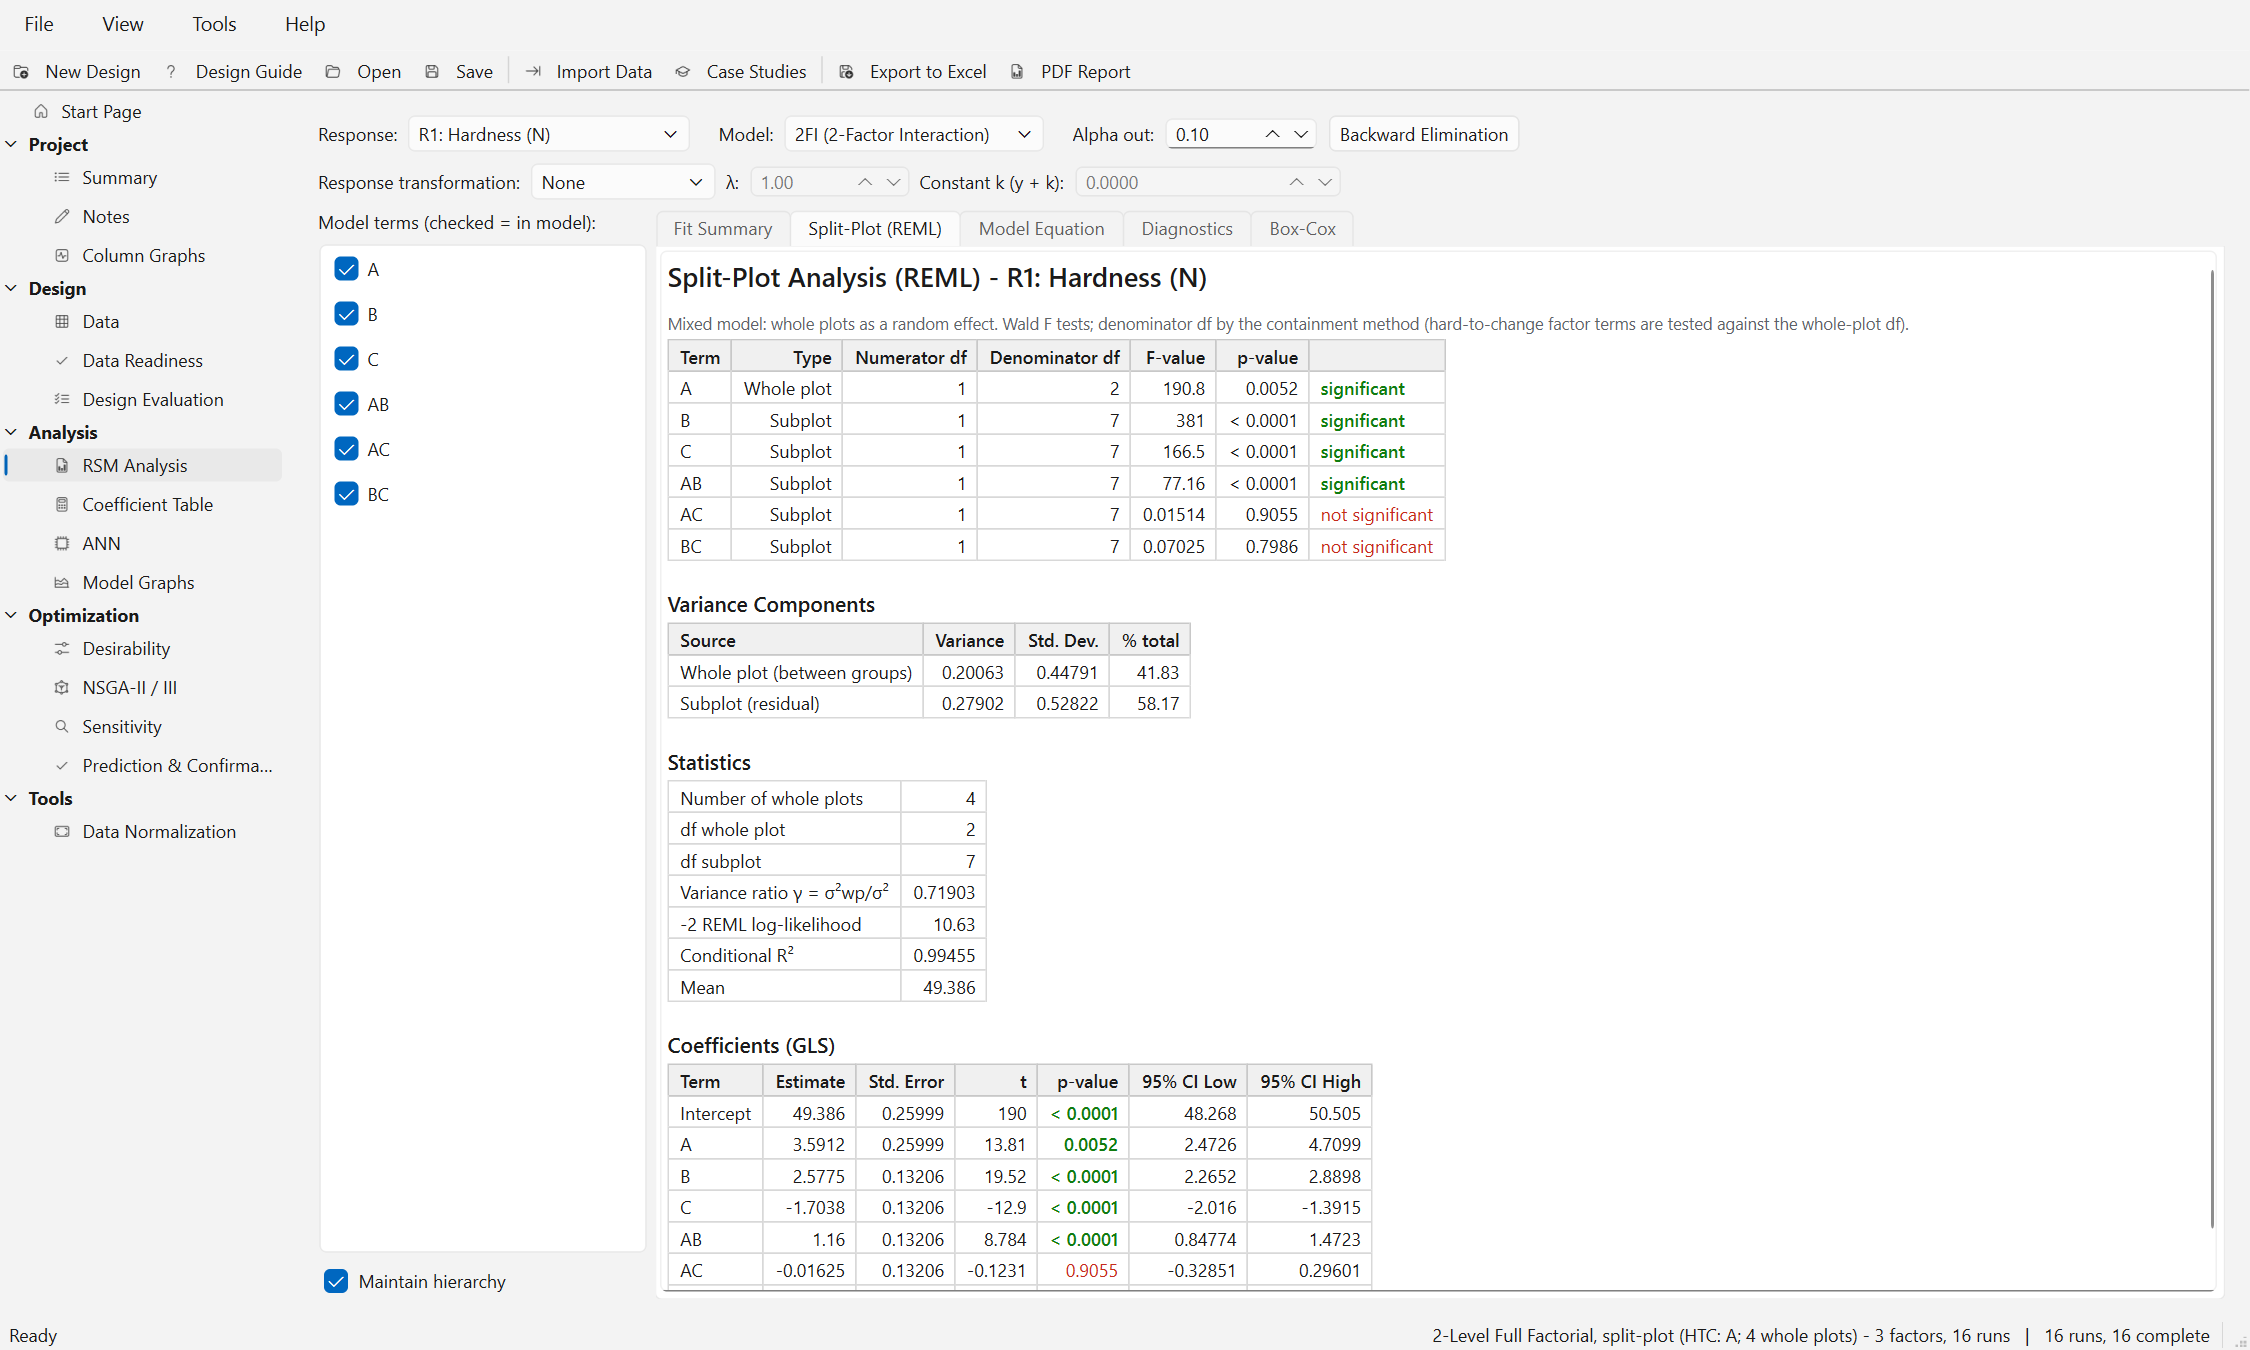
\includegraphics[width=\linewidth]{reml_splitplot.png}
\caption{Split-Plot (REML) sub-tab for the oven hardness case: Wald F tests with whole-plot and subplot
denominator df, variance components and statistics.}
\label{fig:ch05-reml}
\end{figure}

\subsection*{Example: Oven Product Hardness (split-plot)}
Oven Temperature (A) is hard to change; Time (B) and Concentration (C) are easy to change. The $2^3$ design
is replicated twice (16 runs) in 4 whole plots of 4 runs. For the default 2FI model ($p=7$),
\eqref{eq:ch05-dfcont} gives $df_{wp}=4-(1+1)=2$ and $df_{sp}=16-4-(7-1-1)=7$. Results: A (whole plot)
$F=190.8$ on 1 and 2 df, $p=0.0052$; B $F=381.0$, C $F=166.5$, AB $F=77.2$ (subplot, 7 df, all
$p<0.0001$); AC $p=0.9055$ and BC $p=0.7986$. The variance components are $\hat\sigma^2_{wp}=0.2006$
(41.8\%) and $\hat\sigma^2=0.2790$ (58.2\%), $\gamma=0.719$, $-2\ell_R=10.63$, conditional R² 0.99455. Although
A has the largest $F$ after B, its p-value is the largest of the active terms because it is judged against
only 2 df: the experiment has just 4 independent oven settings. Backward elimination at 0.10 removes AC and
BC.

\section{Coefficient Table page}\label{sec:ch05-coeftable}

\subsection*{Purpose}
The \ui{Coefficient Table} page (navigation group \ui{Analysis}) shows the coded coefficients of all
responses side by side, so you can see at a glance which factor affects which response and in which
direction.

\subsection*{How to use}
Open the page; it always reflects the current model of each response. The only option is the check box
\ui{Show p-values} (default on), which prints the p-value under each coefficient.

\subsection*{Output and how to read it}
\begin{itemize}
  \item Heading ``Coefficient Table (coded factors)''; one row per coefficient label (all responses
        together) and one column per response that has a model. An empty cell means that the term is not in
        that response's model.
  \item Cell color by the p-value of the coefficient: $p<0.01$ green, $p<0.05$ light green, $p<0.10$
        yellow; the intercept is never colored. The p-values are two-sided $t$ tests on $n-p$ df for least
        squares, Wald $z$ tests for GLM responses and $t$ tests with the containment df for REML responses
        (Section~\ref{sec:ch05-reml}).
  \item Footer rows: \ui{Transform}, \ui{Model} (order), \ui{p model} (model F test or GLM
        likelihood-ratio test; a dash for REML), \ui{R²} (McFadden R² for GLM, conditional R² for REML),
        \ui{Adj R²}, \ui{Pred R²} and \ui{Used for optimization} (\ui{RSM} or \ui{ANN} with its
        architecture).
  \item Closing note: coefficients are in coded units, so their sizes can be compared across factors; for
        responses that use an ANN the table still shows the RSM coefficients.
\end{itemize}
Because the factors are coded $-1$ to $+1$, a coefficient is half the change of the response from the low
to the high level of that factor (other factors at the center). Signs show conflicts between responses.

\begin{figure}[htbp]\centering
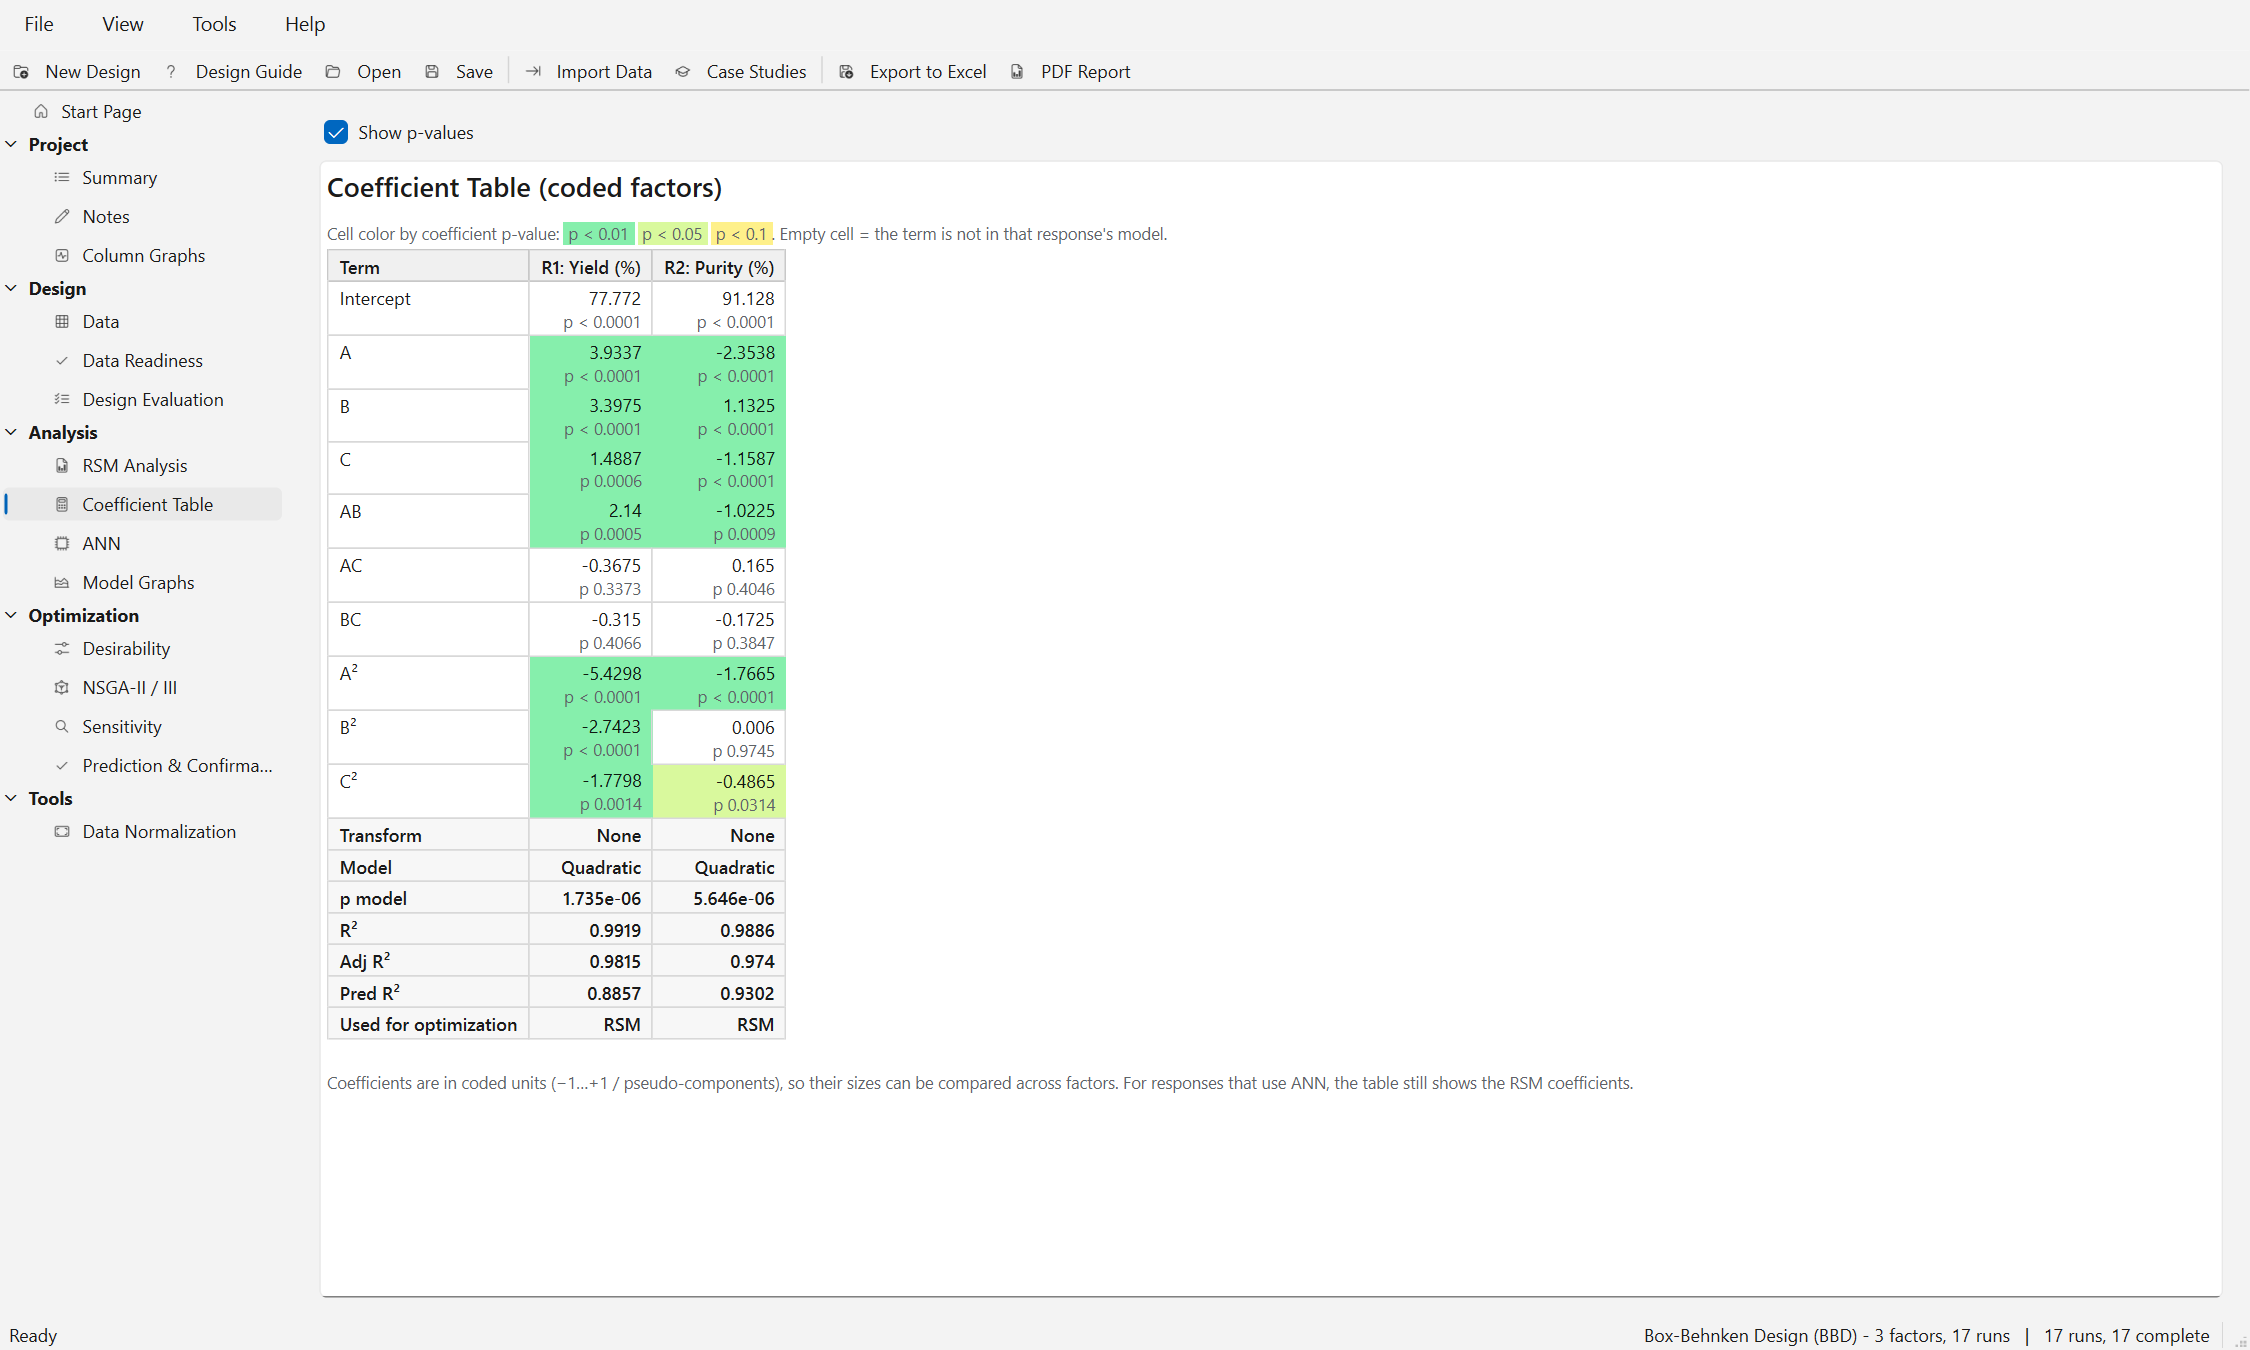
\includegraphics[width=\linewidth]{coefficient_table.png}
\caption{Coefficient Table for the Box-Behnken extraction case (Yield and Purity) with p-values and
p-value colors.}
\label{fig:ch05-coeftable}
\end{figure}

\subsection*{Example}
For the Box-Behnken case (Figure~\ref{fig:ch05-coeftable}) Temperature raises Yield ($A=3.9337$) but lowers
Purity ($A=-2.3538$), while Time raises both ($B=3.3975$ and 1.1325). The curvature in Temperature is strong
for both responses ($A^2=-5.4298$ and $-1.7665$). AC and BC are uncolored for both responses (p 0.34 to 0.41),
and B² of Purity ($p=0.9745$) is a candidate for removal. The conflict in Temperature is the reason why the
two responses must be optimized together (desirability or NSGA-II).

\subsection*{Data export}
Right-click the table for \ui{Copy all tables (for Excel)} or \ui{Export all tables\dots}. The PDF report
includes this table when the project has more than one response.

% Chapter 6: Model Graphs page
\chapter{Model Graphs}\label{sec:ch06-graphs}\label{chap:6}

The \ui{Model Graphs} page (navigation group \ui{Analysis}) draws the fitted model of a response, or of
several responses together, as contour plots, surfaces and effect plots. The graphs show what the
equations of Chapter~\ref{chap:5} mean in the factor space: where the response is high or low, how strongly each
factor acts, whether factors interact, and where all requirements are met at the same time.

\section{Controls and common behavior}\label{sec:ch06-controls}

\subsection*{Purpose}
The page answers the question ``what does the model predict, and where?''. It does not fit anything
itself: it uses the model selected on the \ui{RSM Analysis} page, or the ANN model when the response is
switched to ANN.

\subsection*{How to use}
\begin{enumerate}
  \item Choose the response in \ui{Response:} and the graph in \ui{Type:}.
  \item Choose the factors on the axes (the axis selectors and their labels depend on the graph type,
        Table~\ref{tab:ch06-controls}). If two selectors hold the same factor, the program changes one of
        them automatically.
  \item Set the values of the factors that are not on an axis in the group \ui{Other Factor Values}. The
        graph is a \emph{slice} through the factor space at these values.
  \item Use the plot toolbar to zoom, pan, save the image, copy or export the data
        (Section~\ref{sec:ch06-export}). 3D graphs can be rotated with the mouse.
\end{enumerate}

\begin{table}[htbp]\centering\small
\caption{Controls of the Model Graphs page.}\label{tab:ch06-controls}
\begin{tabularx}{\linewidth}{@{}>{\raggedright\arraybackslash}p{2.6cm} >{\raggedright\arraybackslash}p{4.4cm} >{\raggedright\arraybackslash}p{1.6cm} X@{}}
\toprule
Control & Values & Default & Meaning \\
\midrule
\ui{Response:} & each response & first & Response to plot (not used by Overlay and Desirability, which use all responses with a goal). \\
\ui{Type:} & see Section~\ref{sec:ch06-types} & first type & Graph type. \\
Axis selectors & \ui{X axis:}, \ui{Y axis:}; Interaction: \ui{X axis:}, \ui{Lines (second factor):}; Cube: \ui{X axis:}, \ui{Y axis:}, \ui{Depth axis:}; mixtures: \ui{Top vertex:}, \ui{Left vertex:}, \ui{Right vertex:} & first factors & Factors on the axes. Contour-type graphs and the cube accept only numeric factors. \\
\ui{Contour lines:} & 4--40 & 12 & Number of contour levels (contour, desirability and POE graphs). \\
\ui{Other Factor Values} & one control per factor not on an axis & see text & Values at which the slice is taken. Title \ui{Other Components (Actual Units)} for mixtures, \ui{Reference Levels} for All Factors and \ui{Reference Point} (one control for every factor) for Perturbation. \\
\bottomrule
\end{tabularx}
\end{table}

\paragraph{Slice controls.} A numeric factor gets a spin box in actual units. Its range runs from the
smaller of the data minimum and the low level to the larger of the data maximum and the high level, so axial
points of a CCD can be reached. The default is the middle of the range, $(\text{low}+\text{high})/2$; for
mixture components it is the design centroid in actual units. The step is 1/20 of the range, with 4
decimals for ranges below 10 and 2 decimals otherwise. A categoric factor gets a list of its levels; the
default is the first level. The values are kept when you change the graph type.

\paragraph{Note below the controls.} Every graph adds ``Red points = design runs in this slice (number =
replicate count).'' For process designs the contour, surface, overlay and desirability graphs add ``Graph
range = levels -1 to +1. Gray area = outside the constraints.'' Mixture designs add ``Mixture graphs are
drawn in pseudo-component space.'' Some types add their own sentence (given in the sections below).

\paragraph{Model source (RSM or ANN).} Each response uses the model chosen for it: RSM by default, or the
ANN when \ui{Use this response's ANN for graphs, optimization, NSGA-II \& prediction} is checked on the
\ui{ANN} page (or \ui{ANN} is chosen in the \ui{Model} column of the \ui{Desirability} page). The response
label then ends in ``[ANN]''. ANN models have no confidence bands, and their POE uses the mean squared error
of the network over all data.

\paragraph{Messages.}
\begin{itemize}
  \item ``This graph needs more numeric factors.'' The type needs more numeric factors than the design has
        (for example a cube plot with two numeric factors).
  \item ``\dots{} Enter response data, then check Analysis.'' No model can be computed yet (the first line
        gives the reason).
  \item ``No criteria yet. Choose response goals and limits on the Desirability page.'' Overlay and
        Desirability need goals; they are set on the \ui{Desirability} page.
  \item ``This slice lies entirely outside the design region. Change the values of the other
        factors/components.'' The slice values violate the bounds or the linear constraints everywhere.
\end{itemize}

\section{The slice grid (theory as implemented)}\label{sec:ch06-grid}

\paragraph{Process designs.} Contour-type graphs evaluate the model on a $60\times60$ grid over the coded
square $[-1,1]^2$ of the two axis factors, with all other factors at the slice values. The axes are labeled
in actual units. Points that violate a linear constraint are outside the feasible region: the region is
drawn grey and the plots are clipped with the exact feasible polygon, computed from the bounds and the
constraints.

\paragraph{Mixture designs.} Ternary graphs evaluate the model on a triangular lattice of resolution 60
over the three chosen components (in pseudo-components), scaled to $1-\sum(\text{other components})$ when
the mixture has more than three components. If less than 20\% of the lattice is feasible, the resolution is
raised to 180. A point with pseudo-components $(a,b,c)$ (top, left, right vertex) is drawn at
$X=c+a/2$, $Y=a\sqrt3/2$. Grid lines of each component are labeled in actual units. When the feasible
region is small, the view zooms in on it, with the note ``Zoomed to the feasible region. Numbers on lines =
component amount (actual units).''; otherwise the vertex amounts are written at the corners.

\paragraph{Design points.} Runs whose coordinates off the axes agree with the slice values within $10^{-3}$
(coded) are drawn as red points; a number next to a point gives the number of replicates at that location.
On contour, overlay, desirability and POE graphs the best desirability solution (the first row of the last
desirability result) is drawn as a yellow star labeled ``Optimum'' when it lies within 0.02 (coded) of the
slice.

\paragraph{Confidence bands.} One-factor, all-factor and interaction graphs show the 95\% confidence
interval of the mean response,
\begin{equation}
  \hat y_0\pm t_{0.975,\,n-p}\sqrt{\text{MSE}\,h_0},\qquad h_0=x_0'(X'X)^{+}x_0,
  \label{eq:ch06-ci}
\end{equation}
computed on the transformed scale and back-transformed. For GLM responses the band is
$g^{-1}(\hat\eta\pm1.96\,\text{se}_\eta)$, for split-plot responses it uses the REML covariance of the
coefficients. No band is drawn when the model has no residual degrees of freedom, or for ANN models.

\section{Graph types}\label{sec:ch06-types}

Process designs offer \ui{2D Contour}, \ui{3D Surface}, \ui{One Factor Effect}, \ui{All Factors},
\ui{Interaction}, \ui{Cube Plot}, \ui{Perturbation}, \ui{Overlay (Graphical Optimization)} and
\ui{Desirability Contour}. Mixture and combined mixture-process designs offer \ui{Ternary Contour},
\ui{3D Ternary Surface}, \ui{Trace (Piepel)}, \ui{Overlay (Graphical Optimization)} and
\ui{Desirability Contour}. Both lists end with \ui{Propagation of Error (POE)} when at least one factor has a
standard deviation $\sigma>0$ (Section~\ref{sec:ch06-poe}). Table~\ref{tab:ch06-axes} summarizes the axes.

\begin{table}[htbp]\centering\small
\caption{Axes needed by each graph type.}\label{tab:ch06-axes}
\begin{tabular}{@{}lcc@{}}
\toprule
Graph & Axis factors & Numeric only \\
\midrule
2D Contour, 3D Surface, Overlay, Desirability, POE (process) & 2 & yes \\
One Factor Effect & 1 & no \\
Interaction & 2 & no \\
Cube Plot & 3 & yes \\
Perturbation & all numeric factors & yes \\
All Factors & all factors & no \\
Ternary graphs, Overlay, Desirability, POE (mixture) & 3 components & yes \\
Trace (Piepel) & all components & yes \\
\bottomrule
\end{tabular}
\end{table}

The examples in this chapter use the Box-Behnken extraction case, response Yield, with Temperature on the
X axis, Time on the Y axis and Concentration at 2\%, unless stated otherwise.

\subsection{2D Contour}\label{sec:ch06-contour}
\paragraph{Purpose.} Shows the predicted response over two factors as filled contours, to locate the
optimum region and see the shape of the surface (ridge, saddle, maximum).

\paragraph{Output.} Filled contours of $\hat y$ (original units) with the number of levels from
\ui{Contour lines:}, black contour lines labeled with their value, a color bar, the design points of the
slice and the optimum star.

\paragraph{Example.} Figure~\ref{fig:ch06-contour}: Yield rises toward high Temperature and high Time; the
model maximum in this slice is 80.2\% at about 75 °C and 85 min. The center point is labeled ``5'' (five
replicates).

\begin{figure}[htbp]\centering
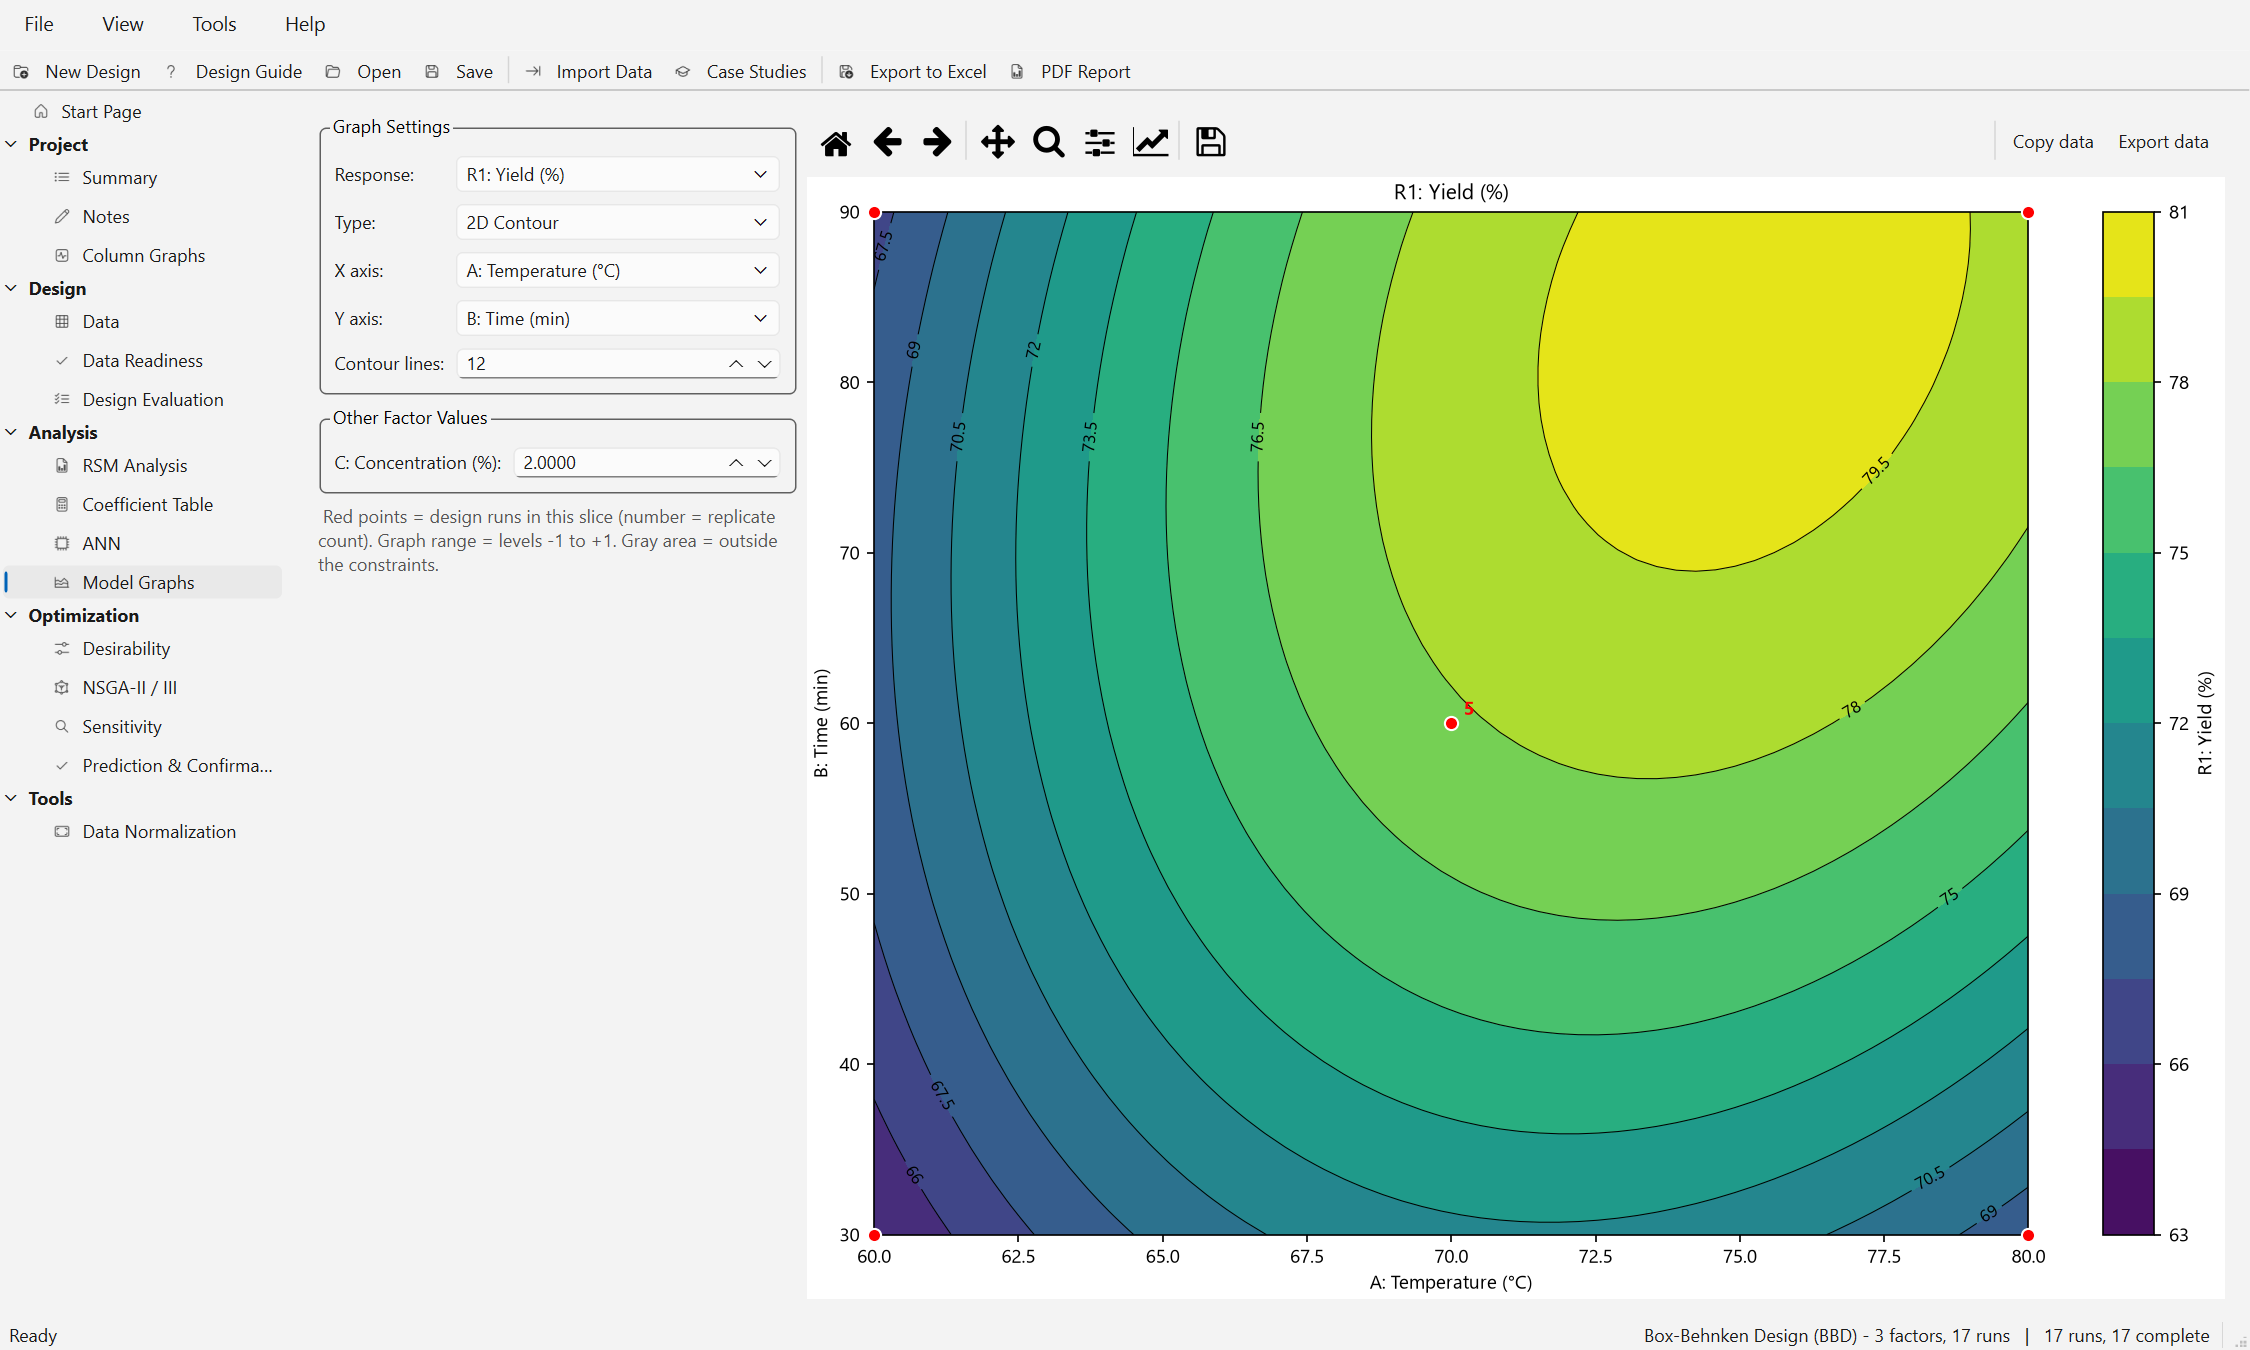
\includegraphics[width=\linewidth]{graph_contour.png}
\caption{2D Contour of Yield (Temperature $\times$ Time, Concentration 2\%) with the design points in the
slice.}
\label{fig:ch06-contour}
\end{figure}

\subsection{3D Surface}\label{sec:ch06-surface}
\paragraph{Purpose.} The same slice as a surface, which makes curvature easy to see.
\paragraph{Output.} A surface of $\hat y$ over the two axis factors (points outside the feasible region are
left out), a color bar, and the observed responses of the runs in the slice as red points, so the distance
between data and surface is visible (Figure~\ref{fig:ch06-surface}).

\begin{figure}[htbp]\centering
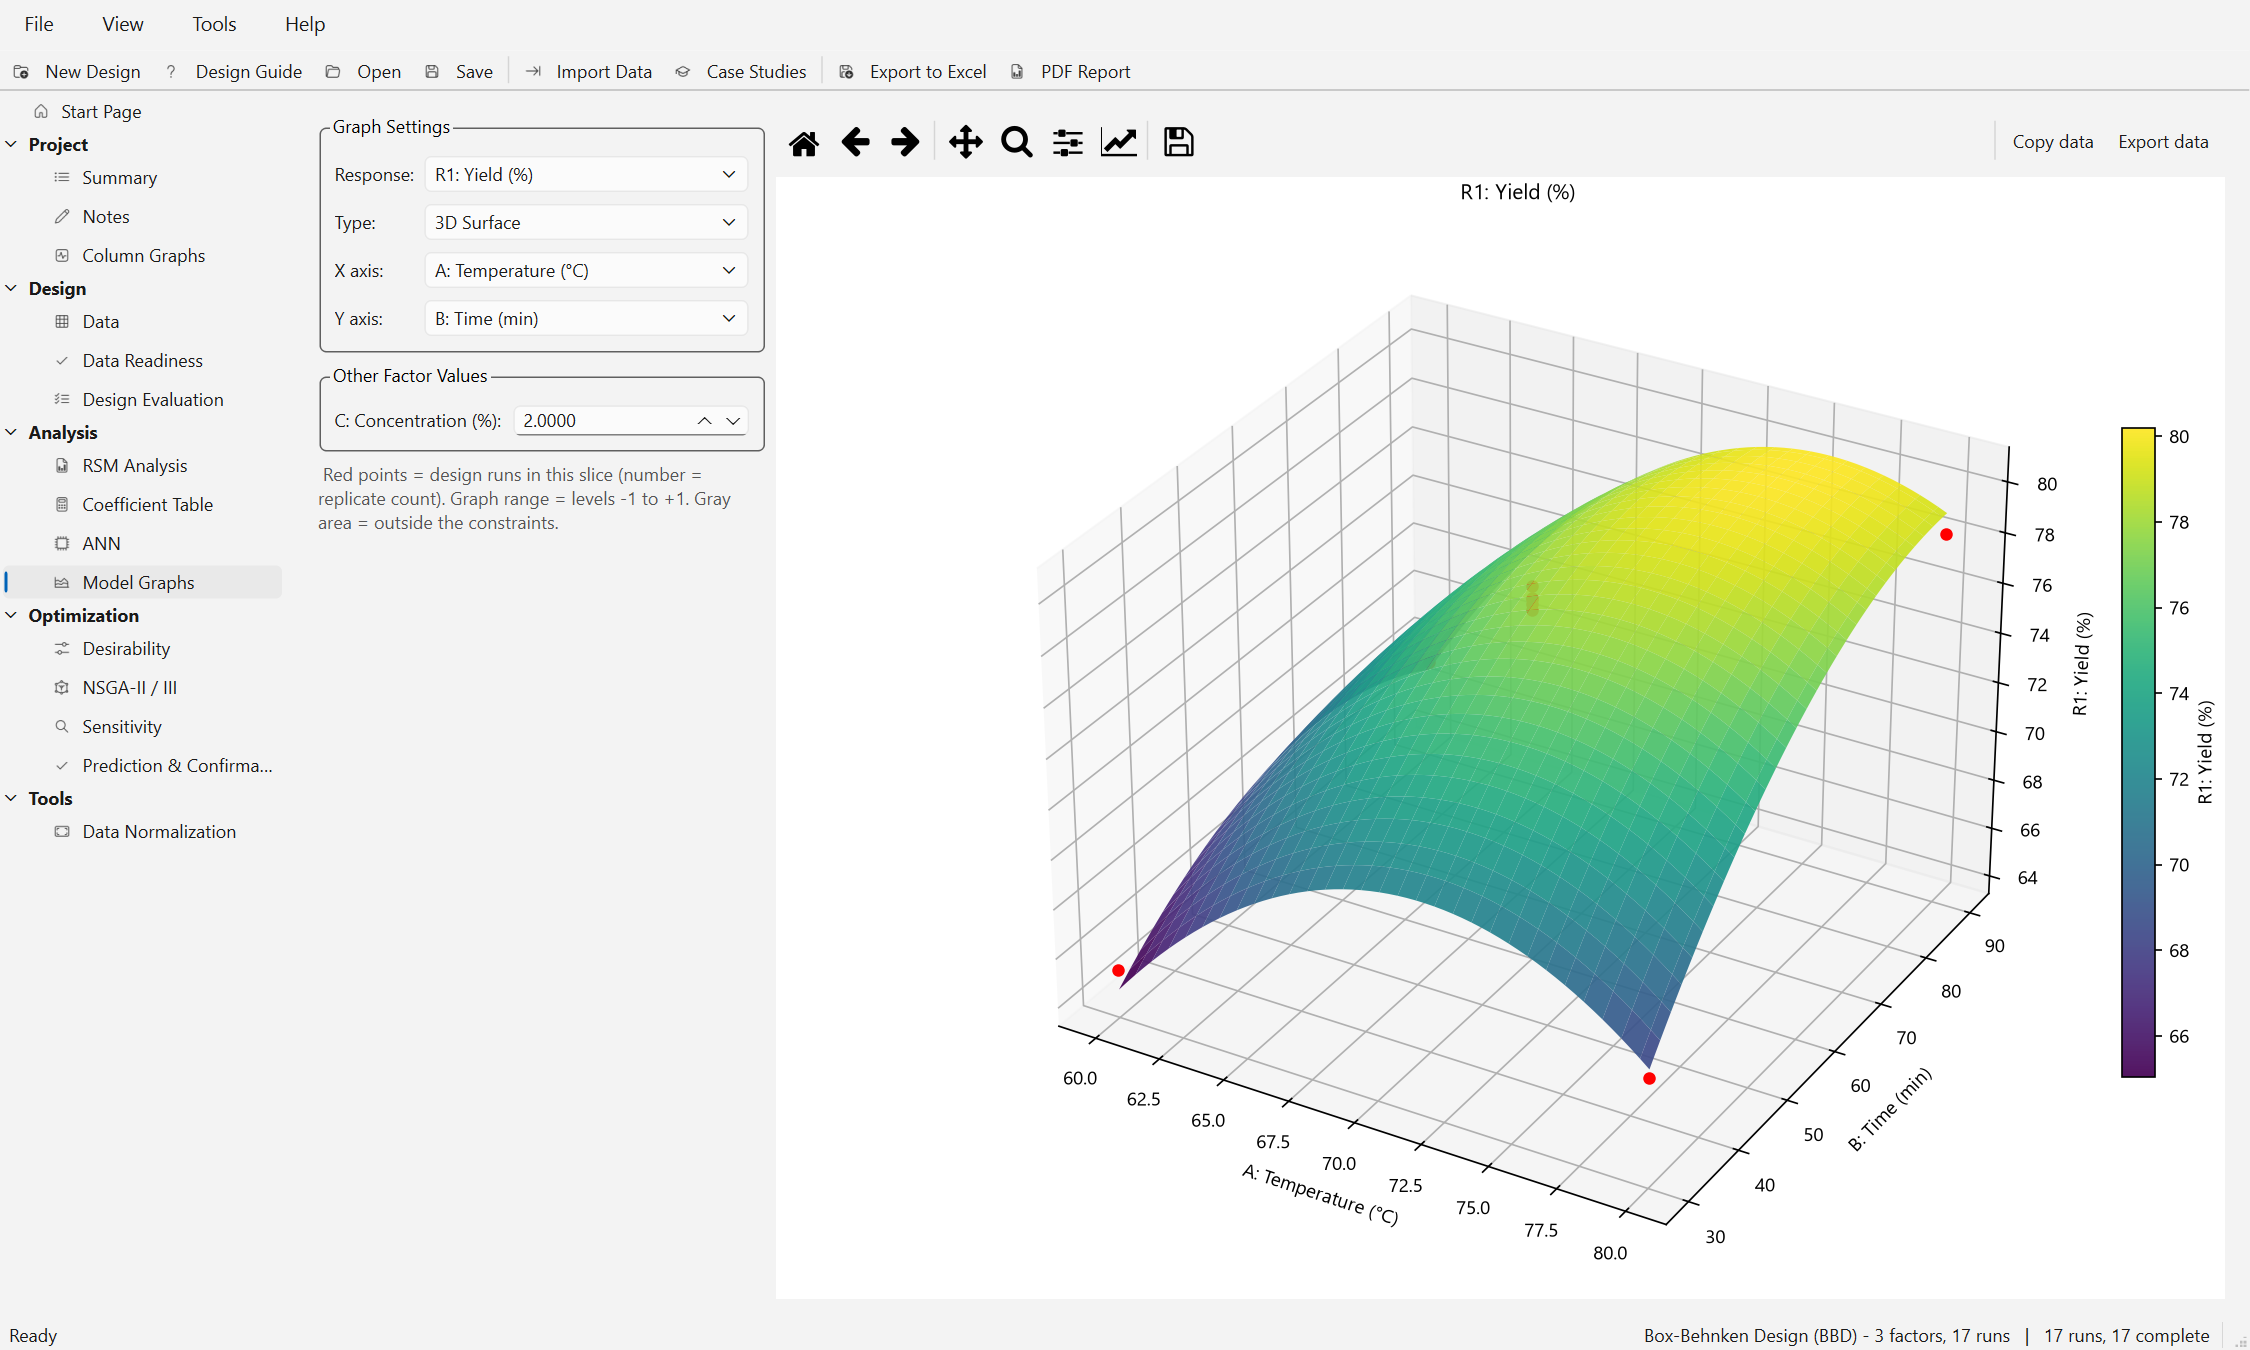
\includegraphics[width=0.85\linewidth]{graph_surface3d.png}
\caption{3D Surface of Yield over Temperature and Time.}
\label{fig:ch06-surface}
\end{figure}

\subsection{One Factor Effect}\label{sec:ch06-oneway}
\paragraph{Purpose.} Shows how the response changes along one factor, with the other factors at the slice
values, and how precisely the model predicts it.
\paragraph{Output.} For a numeric factor: the prediction over the coded range $-1$ to $+1$ (100 points,
axis in actual units) with the 95\% confidence band \eqref{eq:ch06-ci}. For a categoric factor: one point per
level with 95\% error bars. Red points are the runs in the slice. Title ``Effect of \dots''.
\paragraph{Example.} Figure~\ref{fig:ch06-oneway}: Yield against Temperature at Time 60 min and
Concentration 2\% is curved, with a maximum of 78.5\% near 73.6 °C. The five center runs appear at 70 °C.

\begin{figure}[htbp]\centering
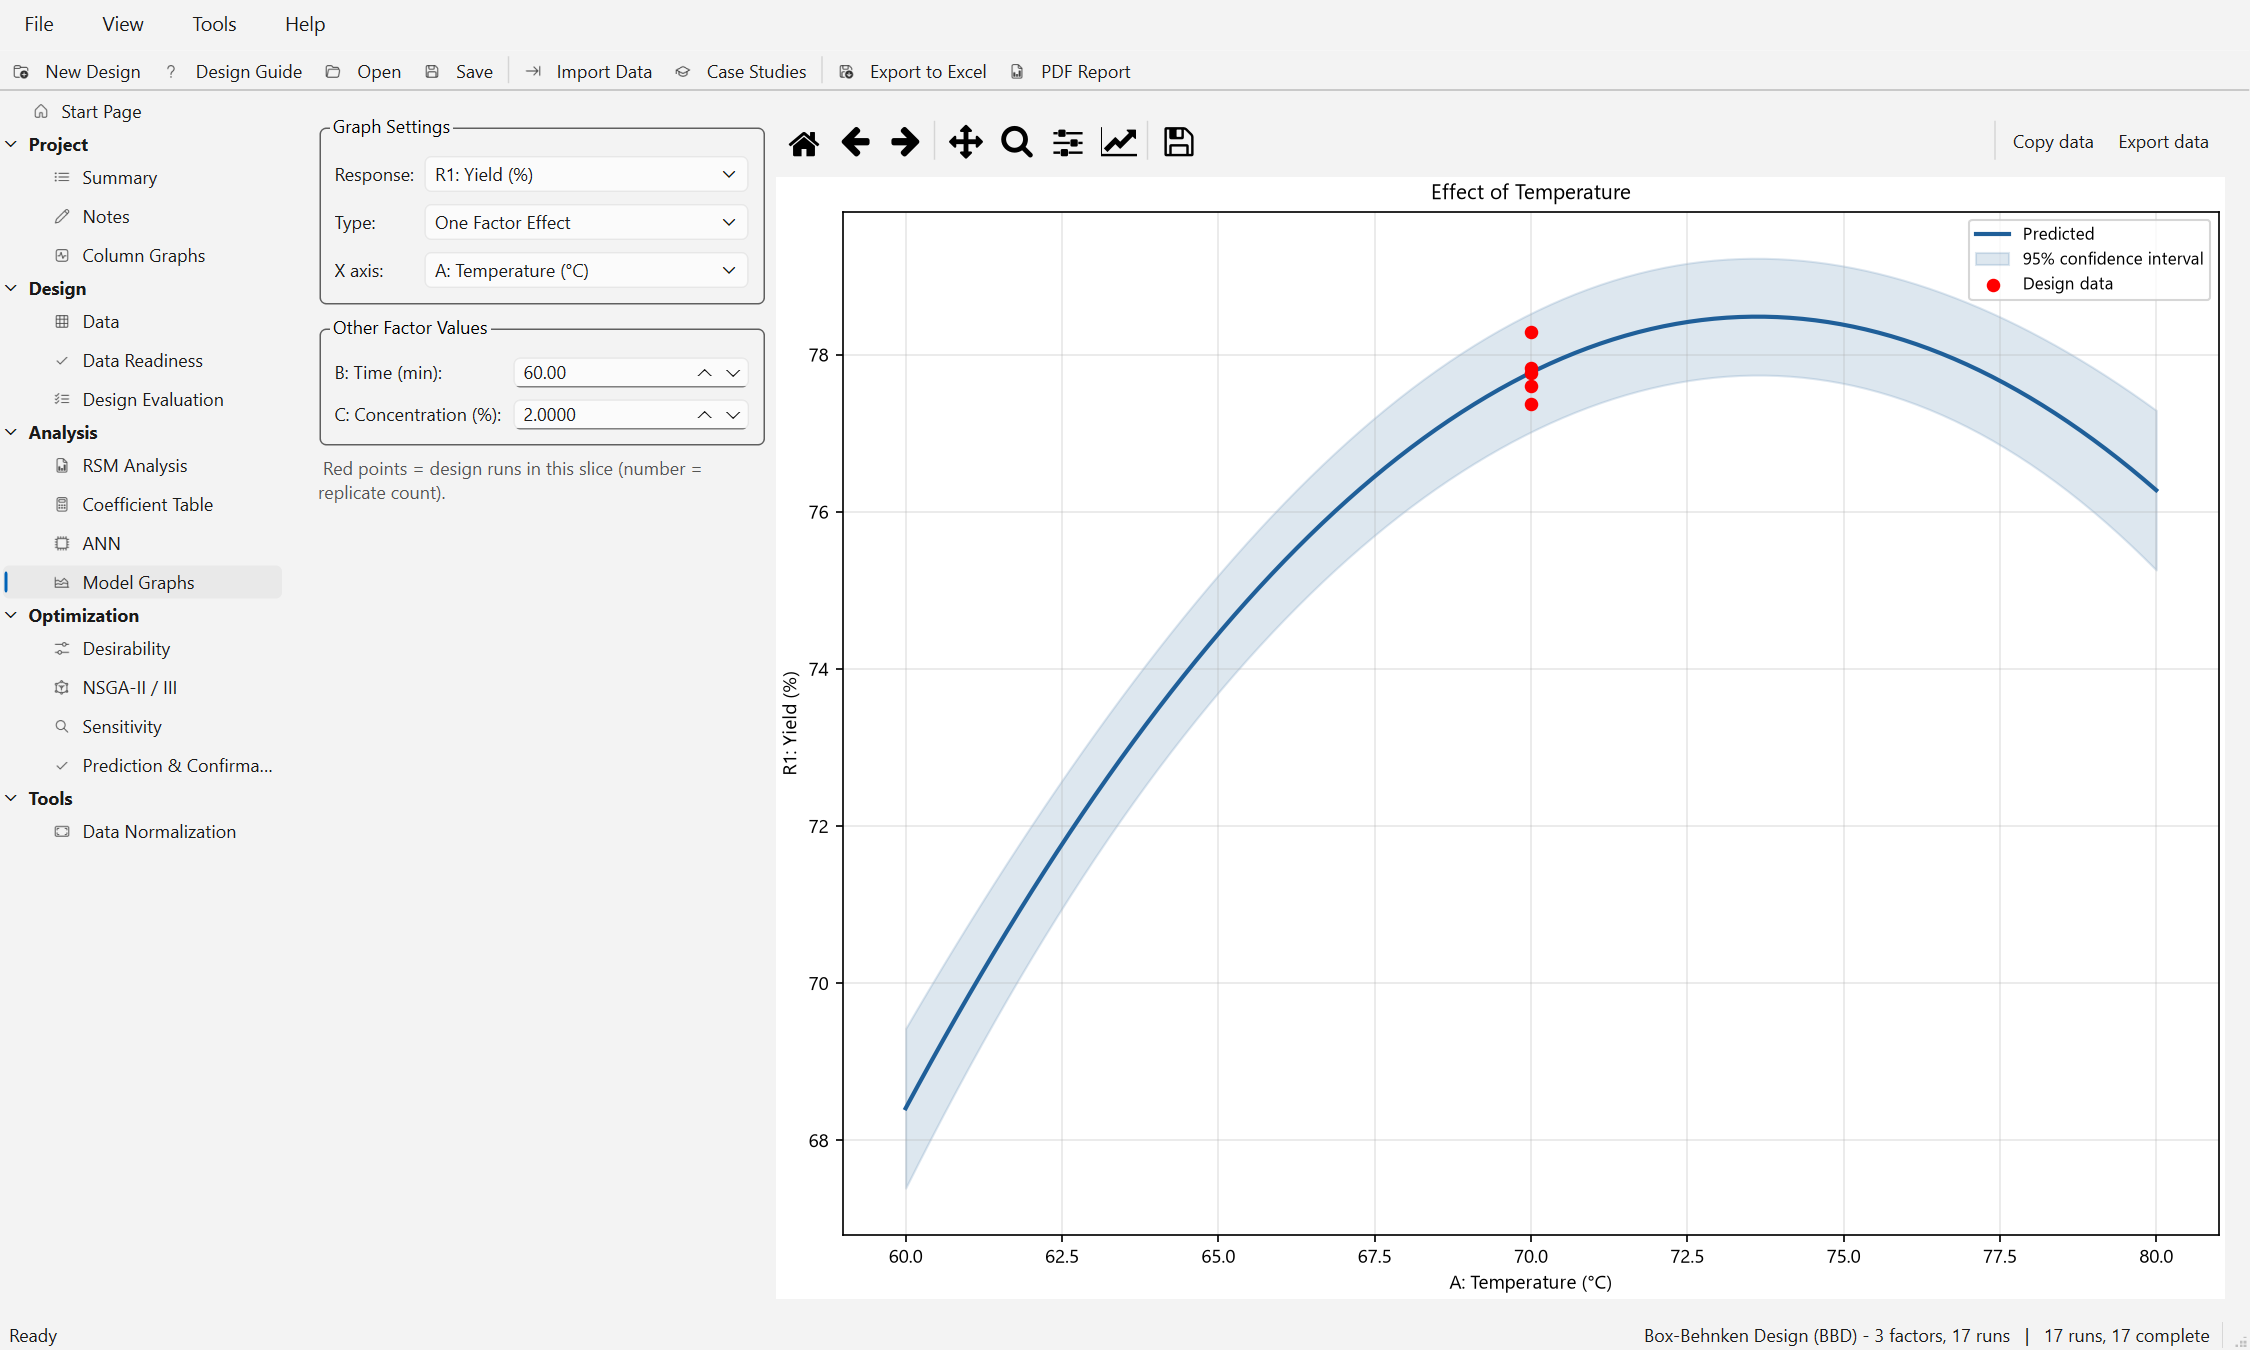
\includegraphics[width=\linewidth]{graph_oneway.png}
\caption{One Factor Effect of Temperature on Yield with the 95\% confidence band.}
\label{fig:ch06-oneway}
\end{figure}

\subsection{All Factors}\label{sec:ch06-allfactors}
\paragraph{Purpose.} One-factor effects of all factors at once, on a shared response axis, so the size of
the effects can be compared directly.
\paragraph{How to use.} Numeric factors are held at the center of their range. For categoric factors the
group \ui{Reference Levels} sets the level at which each one is held in the panels of the other factors
(note: ``Numeric factors are held at the center of their range. Choose below the level at which each
categorical factor is held in the panels of the other factors.'').
\paragraph{Output.} A grid of panels (up to three per row), each with its 95\% band (or error bars for a
categoric factor) and a dotted line at the reference value. The title lists the reference point, for example
``All Factors - other factors at the reference point: Temperature=70, Time=60, Concentration=2 (band = 95\%
CI)''. In Figure~\ref{fig:ch06-allfactors} Temperature has the widest range of Yield and Concentration the
smallest.

\begin{figure}[htbp]\centering
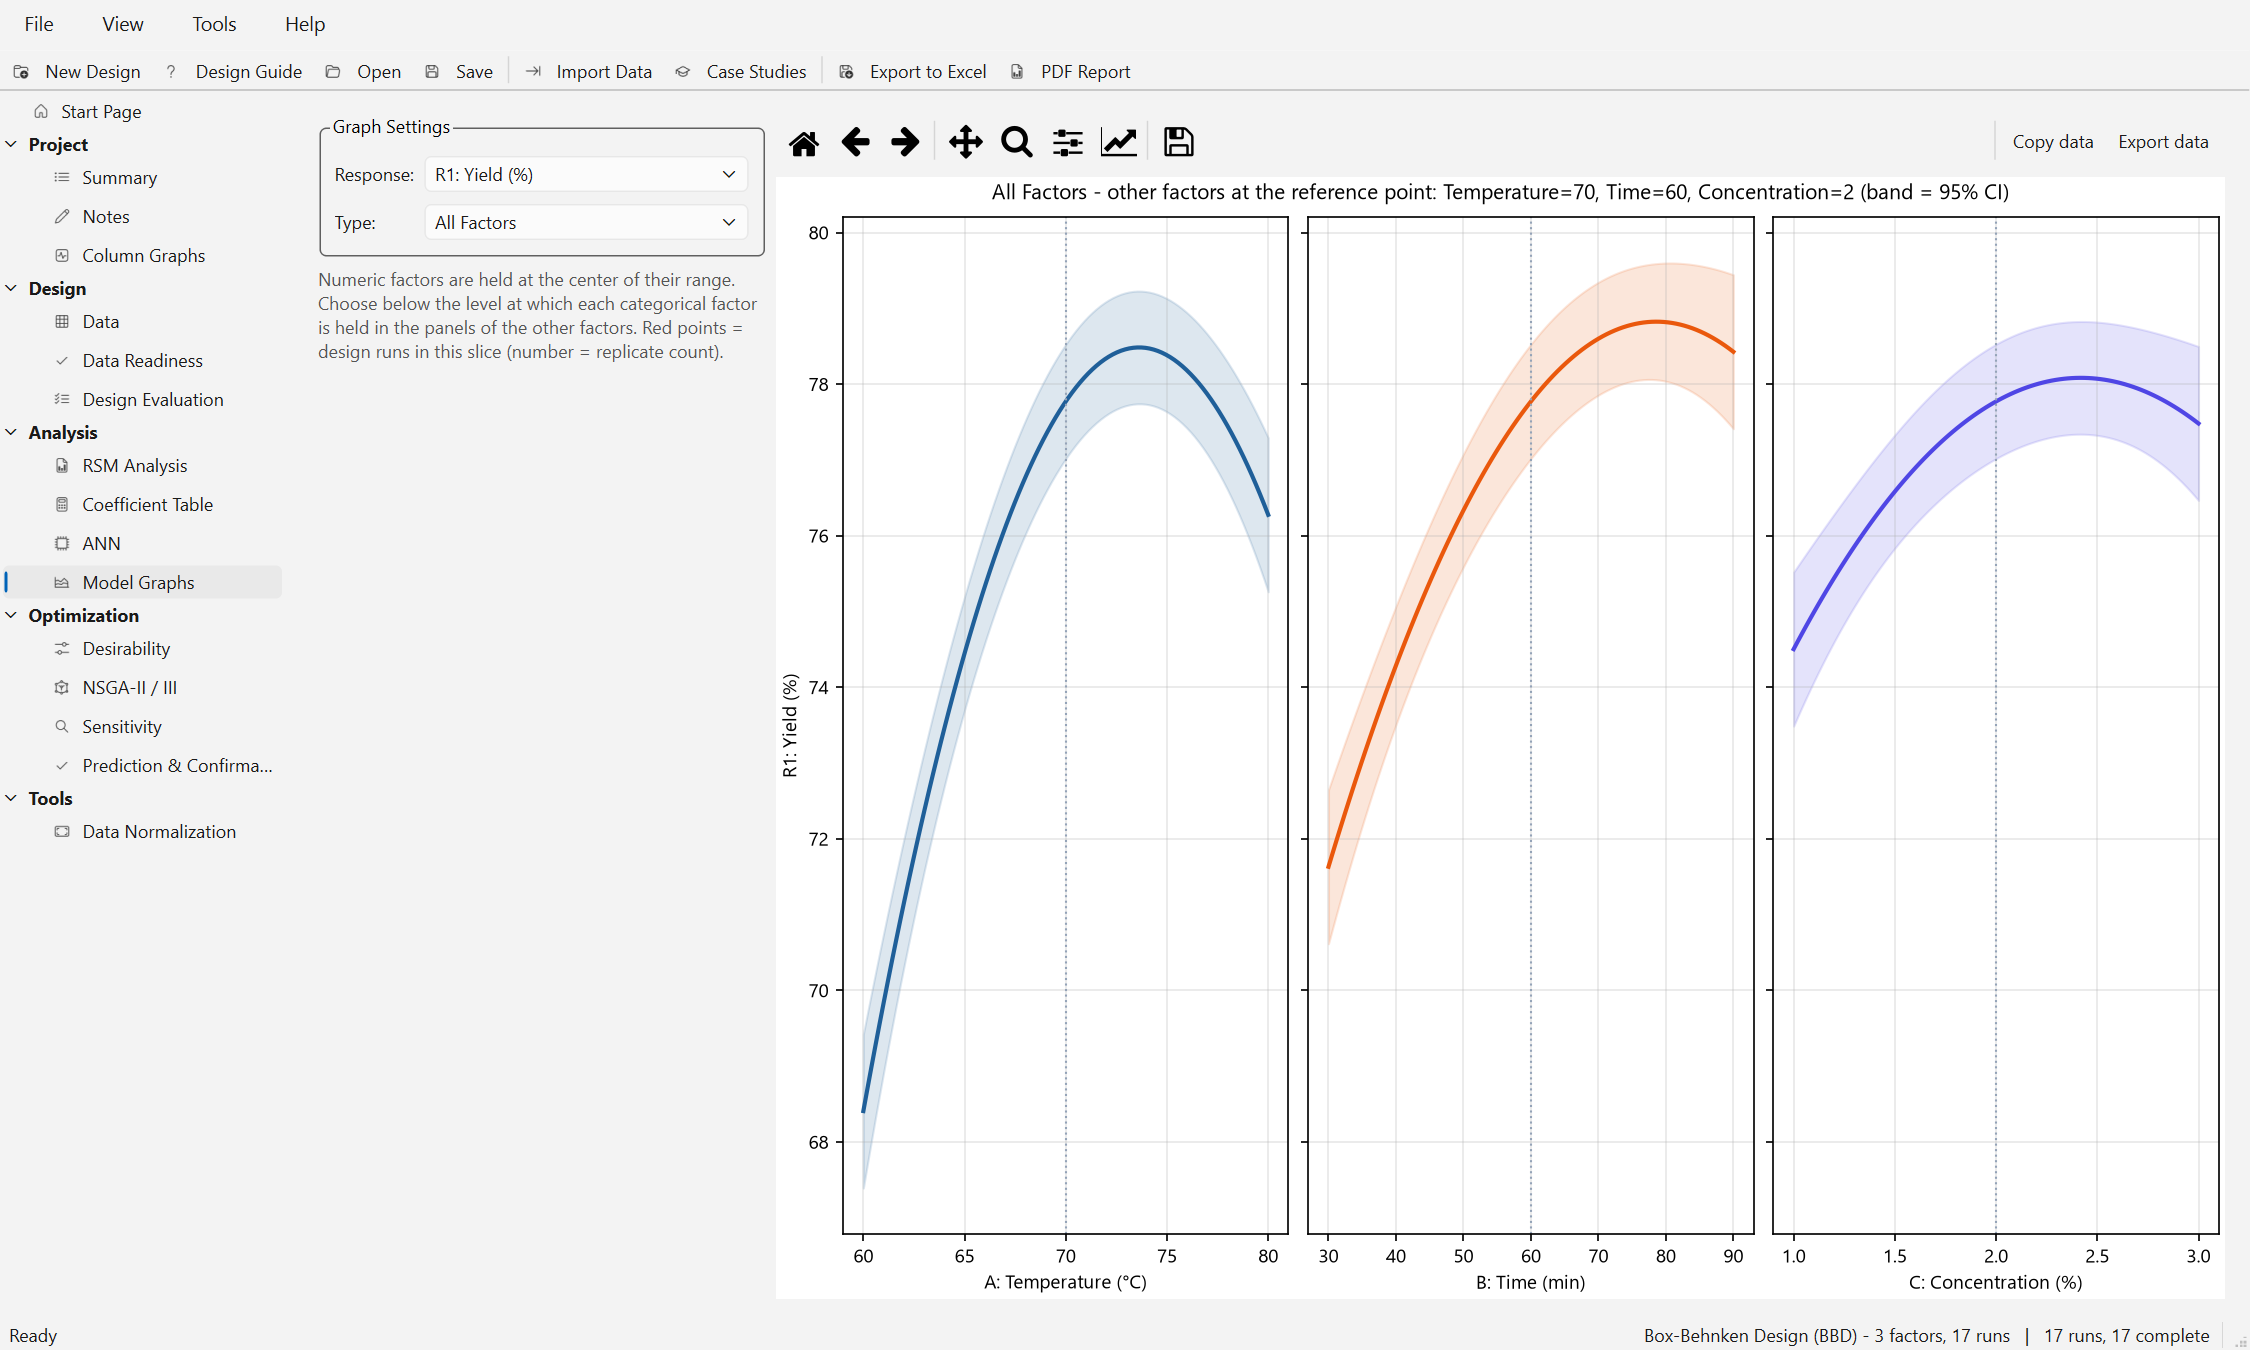
\includegraphics[width=\linewidth]{graph_all_factors.png}
\caption{All Factors graph for Yield: one panel per factor, other factors at the center.}
\label{fig:ch06-allfactors}
\end{figure}

\subsection{Interaction}\label{sec:ch06-interaction}
\paragraph{Purpose.} Shows whether the effect of one factor depends on the level of another.
\paragraph{Output.} The response along the \ui{X axis:} factor, with one line per level of the
\ui{Lines (second factor):} factor: for a numeric factor its low ($-1$) and high ($+1$) level, labeled
``Time low (30)'' and ``Time high (90)''; for a categoric factor one line per level. For a numeric X factor,
95\% error bars are drawn at both ends of each line; for a categoric X factor at every level. Title
``Interaction AB''. Note: ``Non-parallel lines = interaction present. Error bars = 95\% CI.''
\paragraph{Example.} In Figure~\ref{fig:ch06-interaction} the Temperature effect is much stronger at high
Time than at low Time, the AB interaction ($\hat\beta_{AB}=2.14$, $p=0.0005$).

\begin{figure}[htbp]\centering
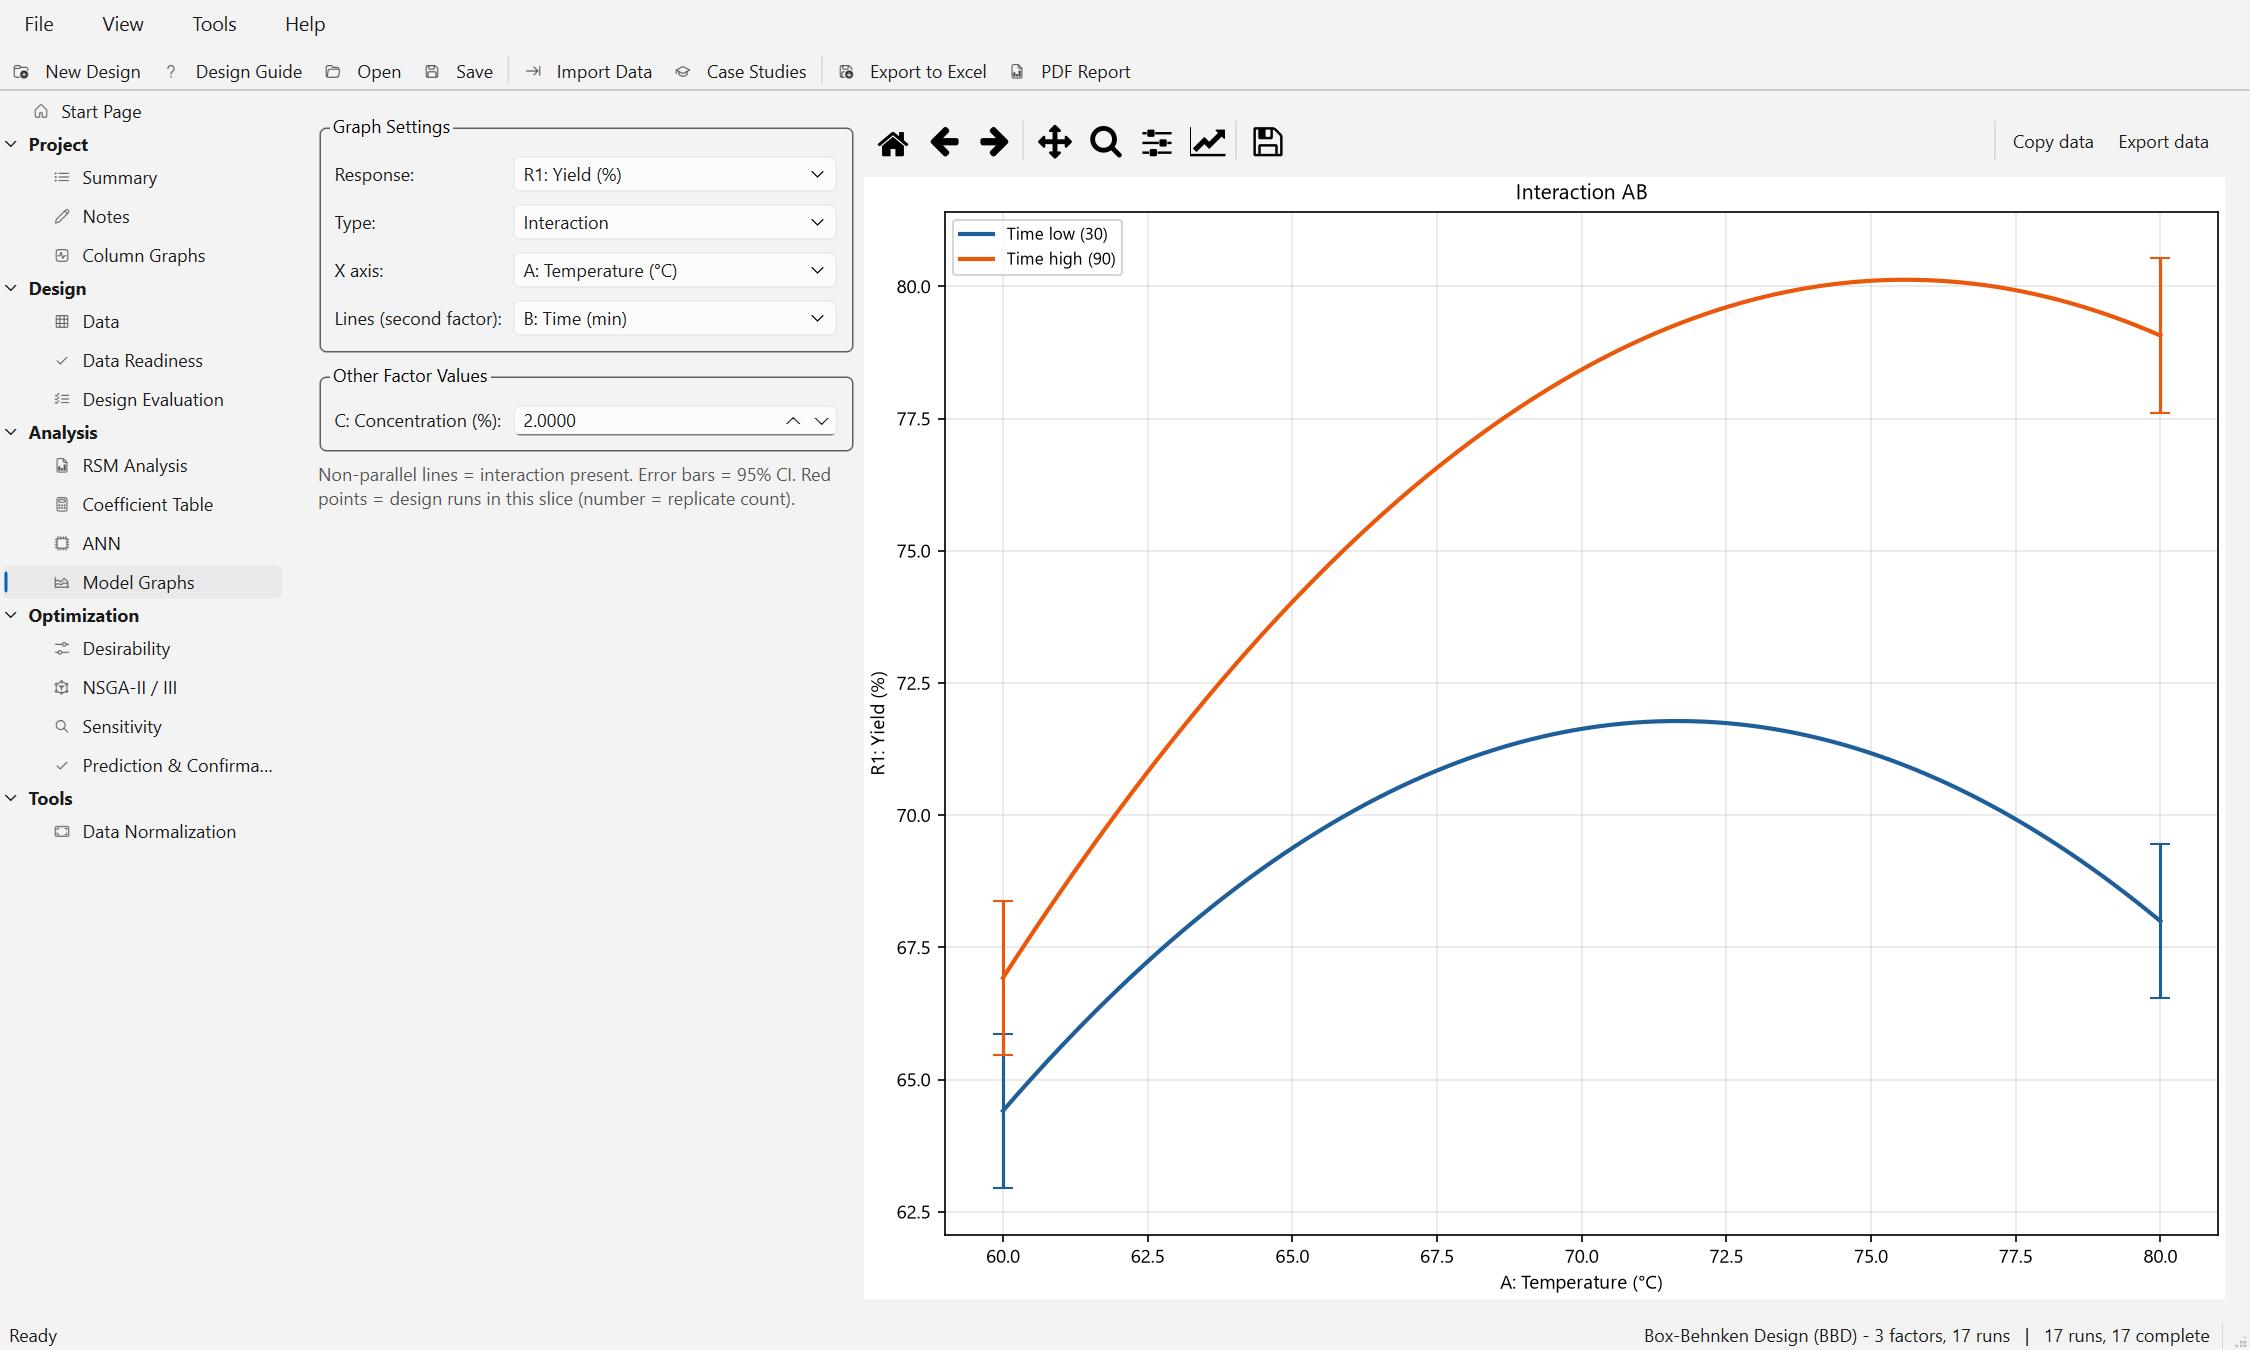
\includegraphics[width=\linewidth]{graph_interaction.png}
\caption{Interaction graph: Yield against Temperature for low and high Time.}
\label{fig:ch06-interaction}
\end{figure}

\subsection{Cube Plot}\label{sec:ch06-cube}
\paragraph{Purpose.} Predictions at the eight corners of three numeric factors, typical for two-level
factorials.
\paragraph{Output.} A cube in oblique projection; each corner shows the predicted response at the
low/high combination (circles colored by value), with the other factors at the slice values. Axis texts give
``low $\rightarrow$ high'' in actual units. Note: ``Corner numbers = predicted response at each low/high level
combination.'' \ui{Copy data} and \ui{Export data\dots} give the table ``Cube corners'' with the three axis
factors in actual units and the predicted response at each of the eight corners; when the design has more factors,
the title lists the values at which the others are held, for example ``Cube corners (D: Solvent = Ethanol)''.
\paragraph{Example.} Figure~\ref{fig:ch06-cube}: predicted Yield ranges from 60.46 (all factors low) to
78.10 (all high).

\begin{figure}[htbp]\centering
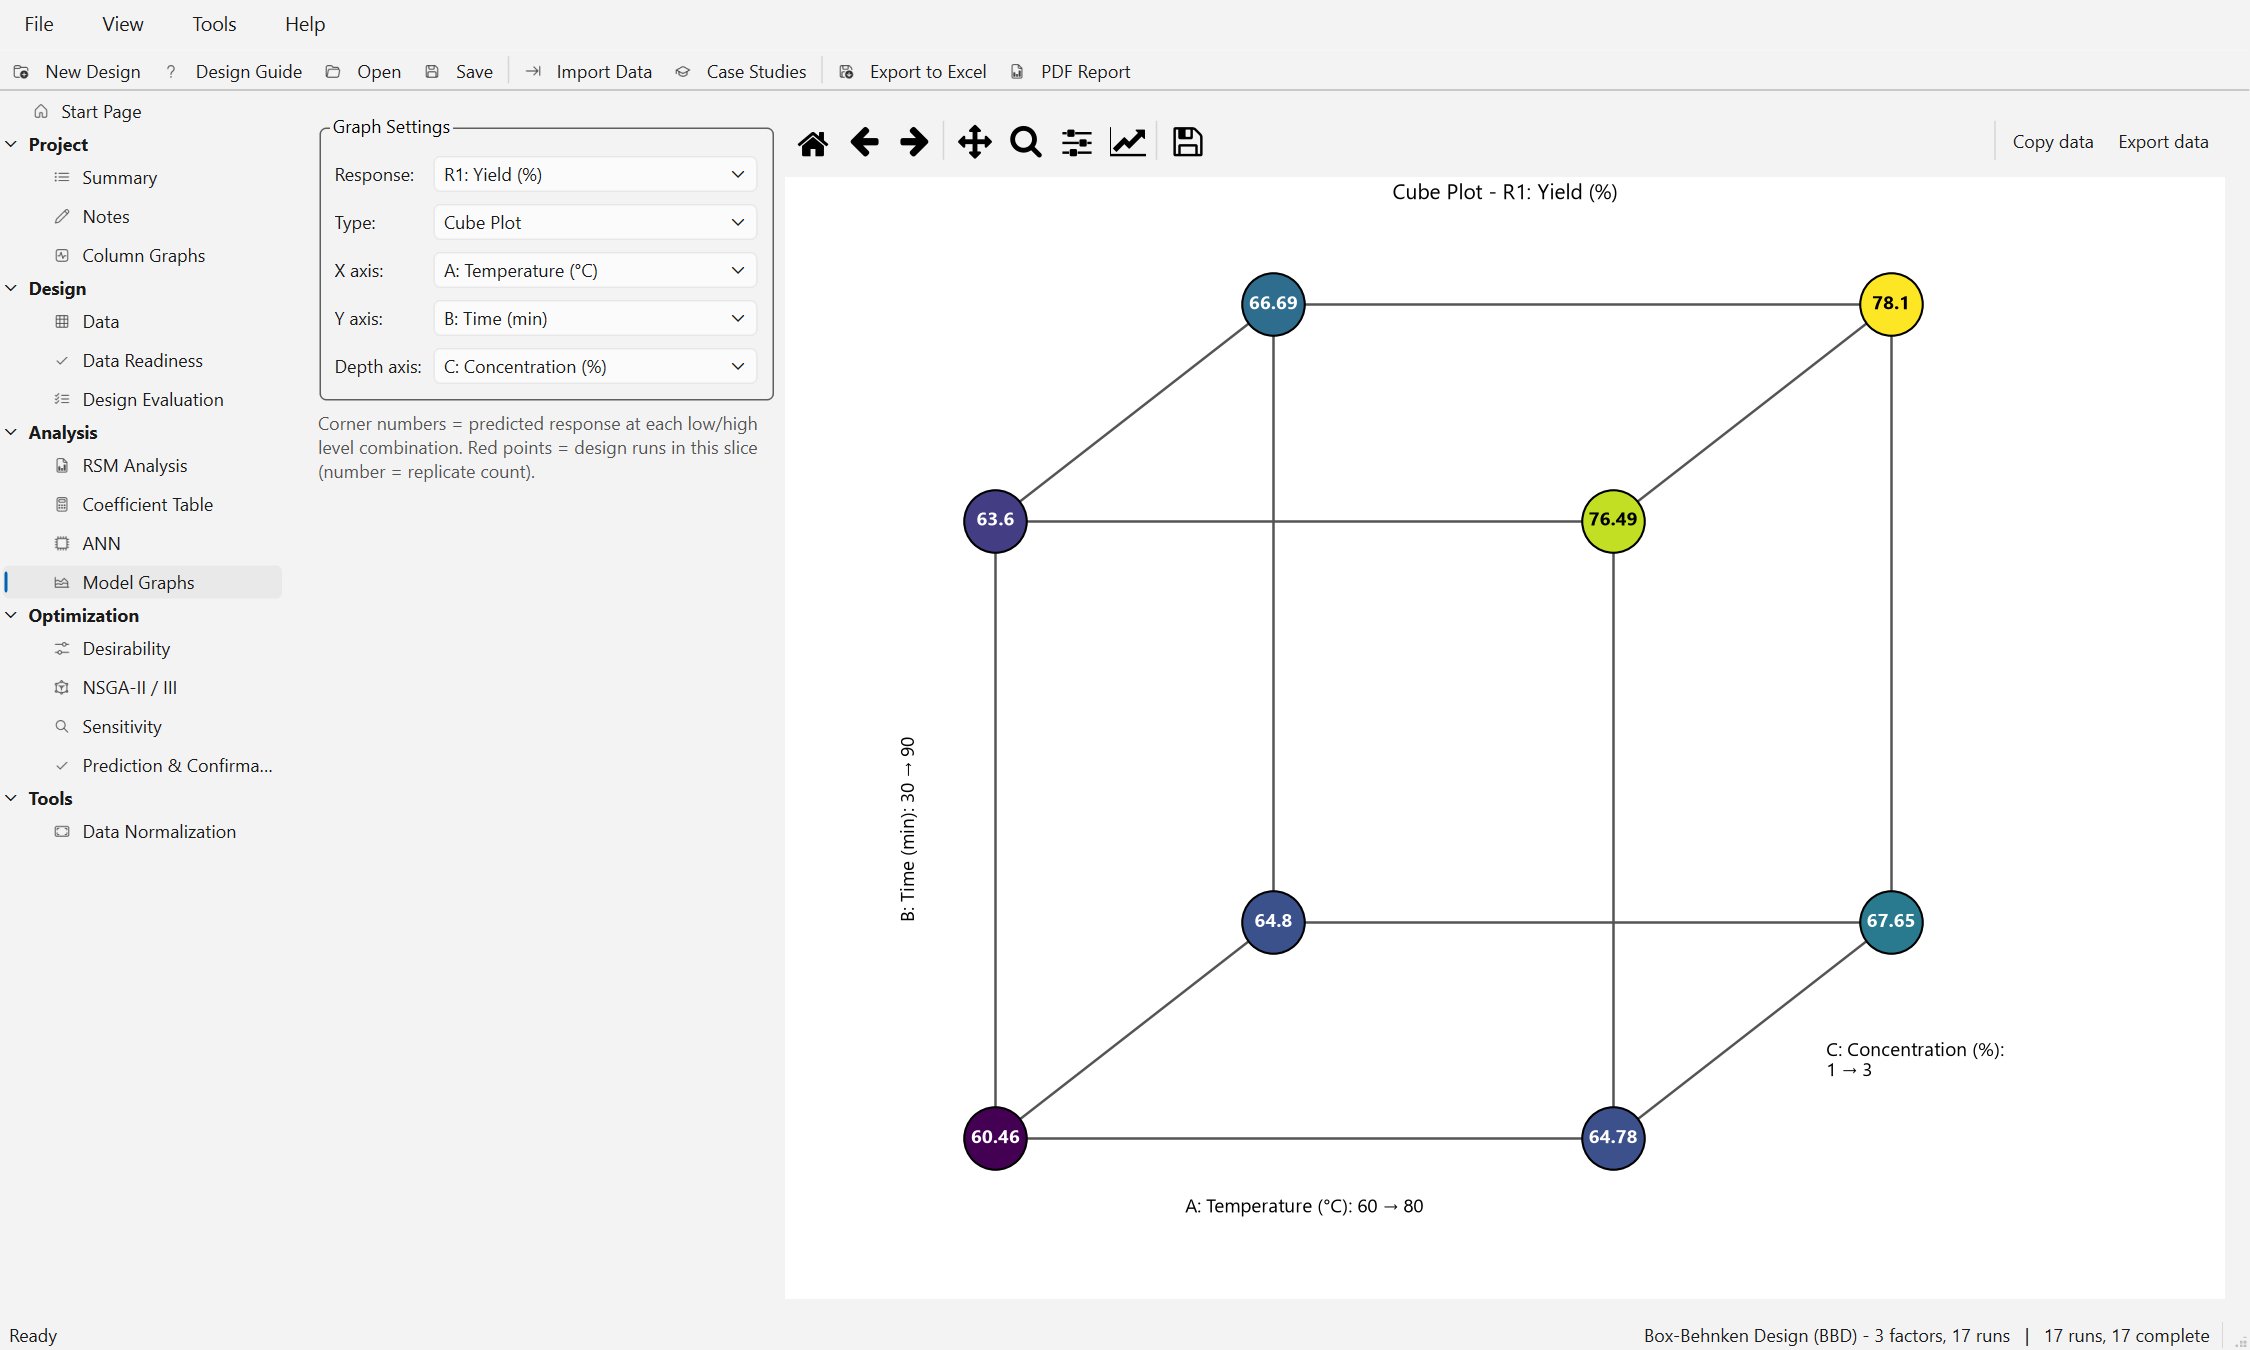
\includegraphics[width=0.85\linewidth]{graph_cube.png}
\caption{Cube Plot of Yield; depth axis Concentration 1 to 3\%.}
\label{fig:ch06-cube}
\end{figure}

\subsection{Perturbation}\label{sec:ch06-perturbation}
\paragraph{Purpose.} Compares all numeric factors around a reference point: a steep trace means a sensitive
factor, a curved trace a quadratic effect, a flat trace an unimportant factor.
\paragraph{How to use.} Set the reference point in the group \ui{Reference Point}, which has a control for
every factor (actual units for numeric factors, a level for categoric factors); it starts at the center of the
ranges.
\paragraph{Output.} Each numeric factor is moved over its whole range, from $-1$ to $+1$ coded units (81
points), while all other factors stay at the reference point, so every trace passes through the reference point.
The x-axis is ``Deviation from reference point (coded units)'': the coded value minus the reference value of that
factor, so a trace runs from $-1-x_{0,i}$ to $1-x_{0,i}$ and covers the full $-1$ to $+1$ span only when the
reference is the center. The title lists the reference values and each trace is labeled with its factor letter.
Note: ``Each numeric factor is moved over its range (-1 to +1) while the other factors stay at the reference point
set below; the x axis is the deviation from the reference value in coded units.'' Not offered for mixture designs
(use the trace plot).
\paragraph{Example.} Figure~\ref{fig:ch06-perturbation}, reference (70 °C, 60 min, 2\%, the center): all
three traces meet at the predicted Yield of the center (77.77); Temperature (A) has the steepest and most curved
trace, Concentration (C) the flattest.

\begin{figure}[htbp]\centering
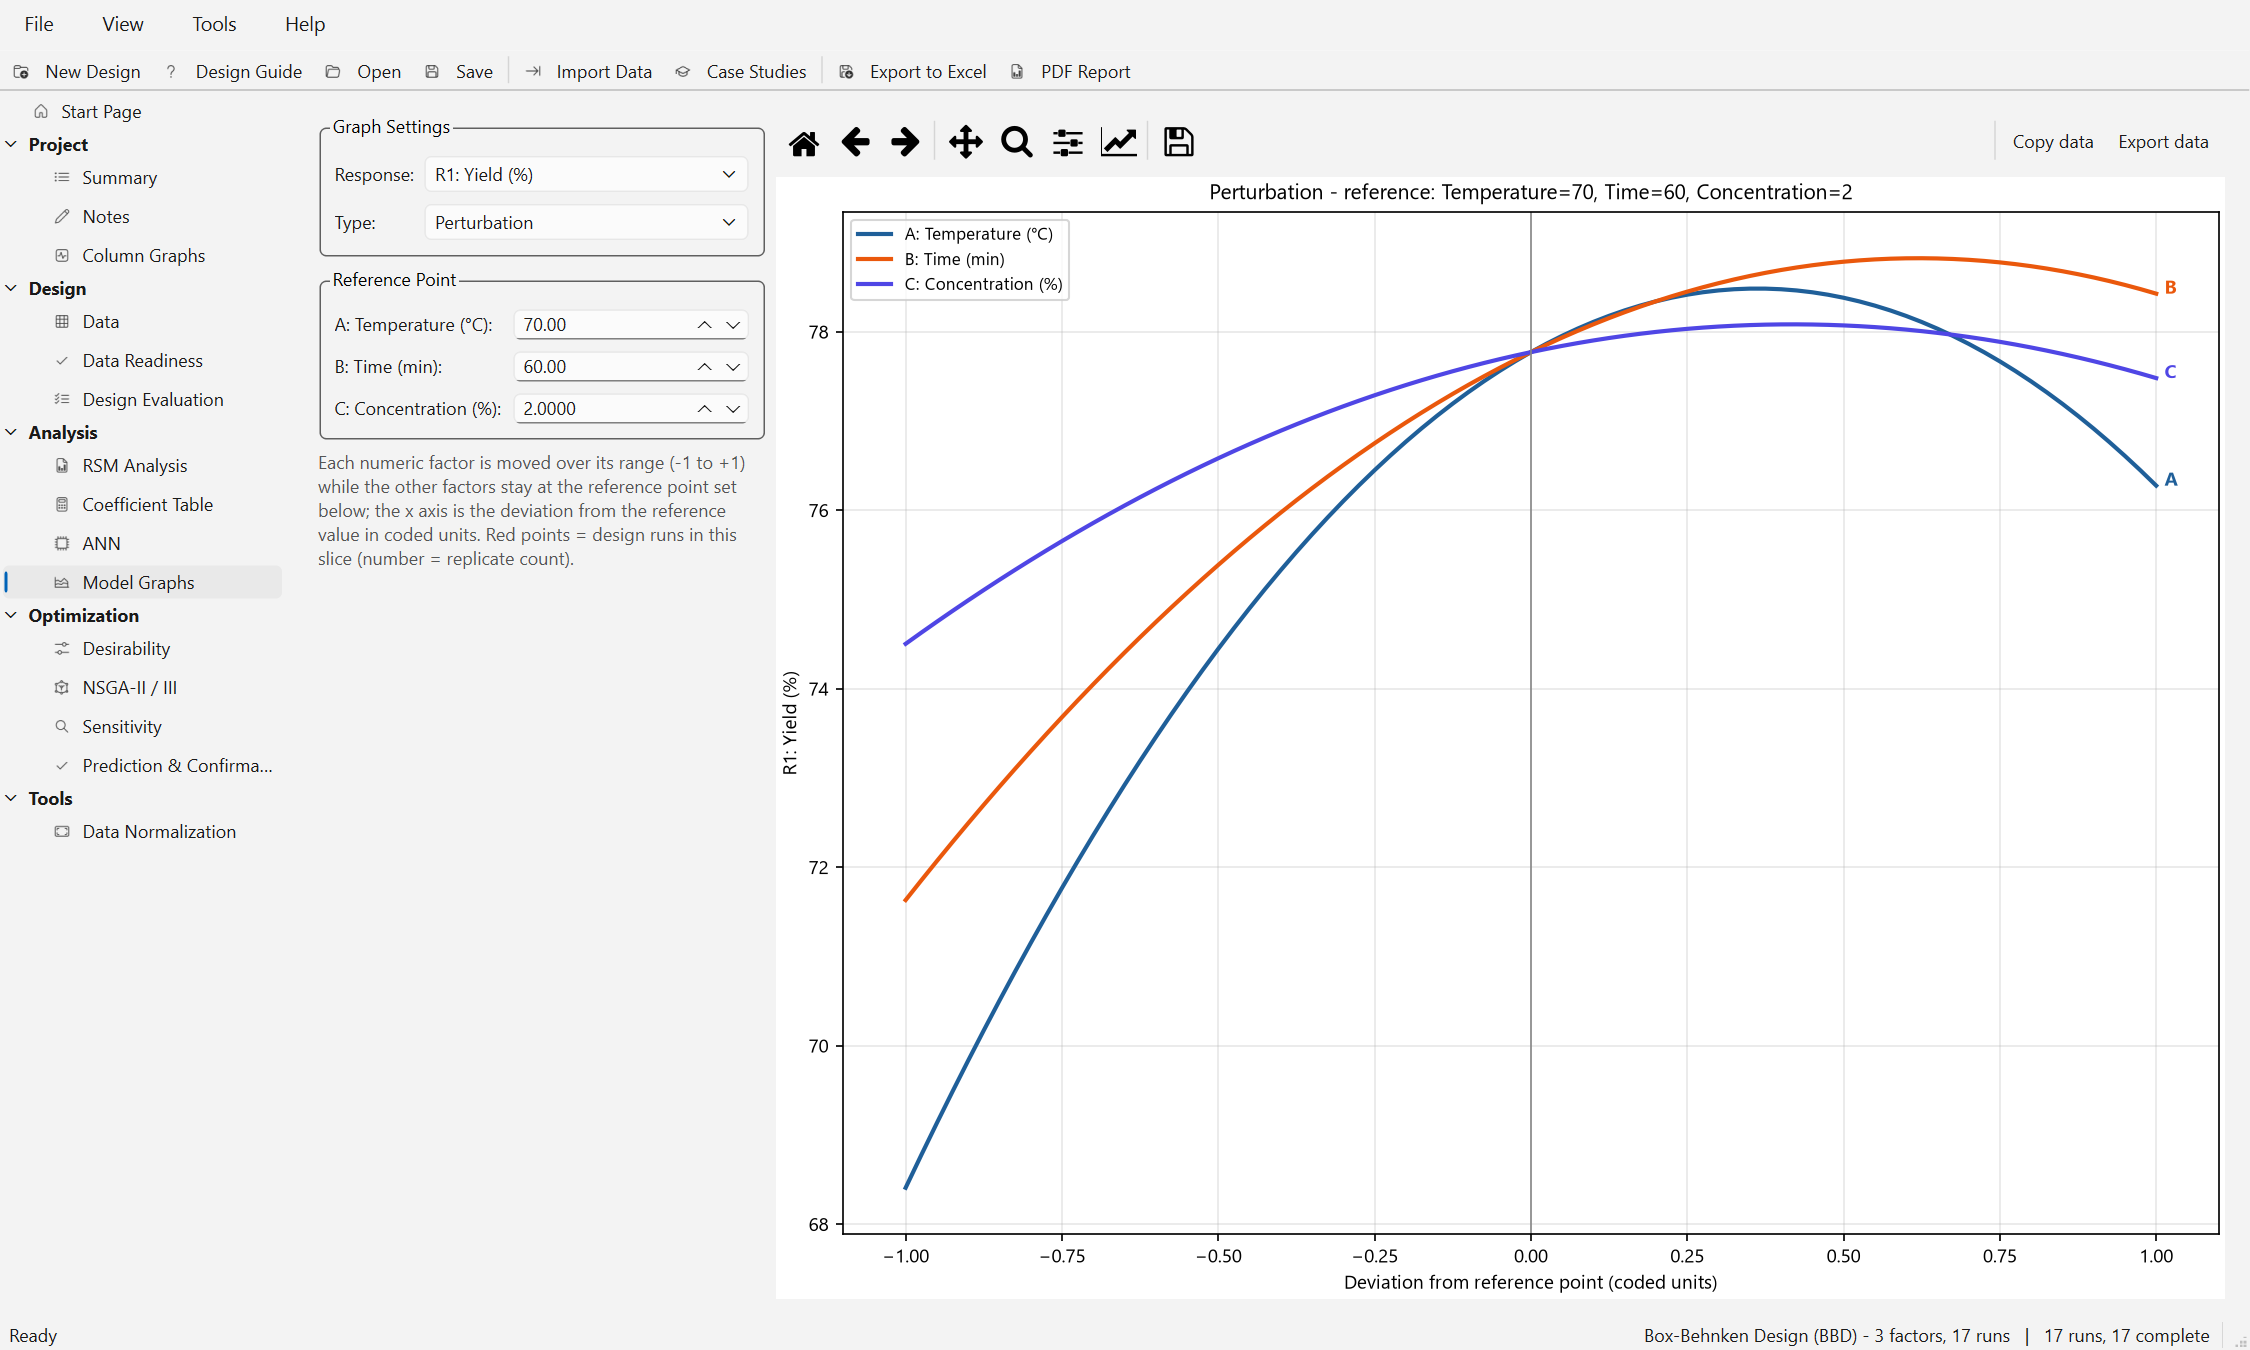
\includegraphics[width=\linewidth]{graph_perturbation.png}
\caption{Perturbation graph for Yield with the \ui{Reference Point} group set to the center of the design
(Temperature 70~°C, Time 60~min, Concentration 2\%).}
\label{fig:ch06-perturbation}
\end{figure}

\subsection{Overlay (Graphical Optimization)}\label{sec:ch06-overlay}
\paragraph{Purpose.} Shows where all responses meet their limits at the same time (the ``sweet spot'').
\paragraph{How to use.} On the \ui{Desirability} page give each response a goal and its \ui{Lower Limit} and
\ui{Upper Limit}. Every response with a goal other than none is used, with the model selected for it.
\paragraph{Theory.} A grid point is acceptable when $L_j\le\hat y_j\le H_j$ for every such response $j$; the
acceptable area is yellow, the rest light grey, and points outside the bounds or constraints darker grey.
Each limit that falls inside the plotted range is drawn as a contour line labeled ``name: value''. Title
``Overlay Plot - yellow = meets all criteria'', with ``(NONE)'' added when no point of the slice qualifies.
Note: ``Each response's limits are taken from the Desirability page (Lower \& Upper Limit for responses with
a goal selected). Yellow area = all responses meet their limits.''
\paragraph{Example.} Figure~\ref{fig:ch06-overlay} uses Yield 75 to 78.29 and Purity 89 to 93.6. With the
goal \emph{maximize}, the upper limit of Yield is the largest observed value (78.29), so the area where the
model predicts more than 78.29 is excluded: it appears as a hole inside the yellow band. Raise the upper
limit if higher values are welcome.

\begin{figure}[htbp]\centering
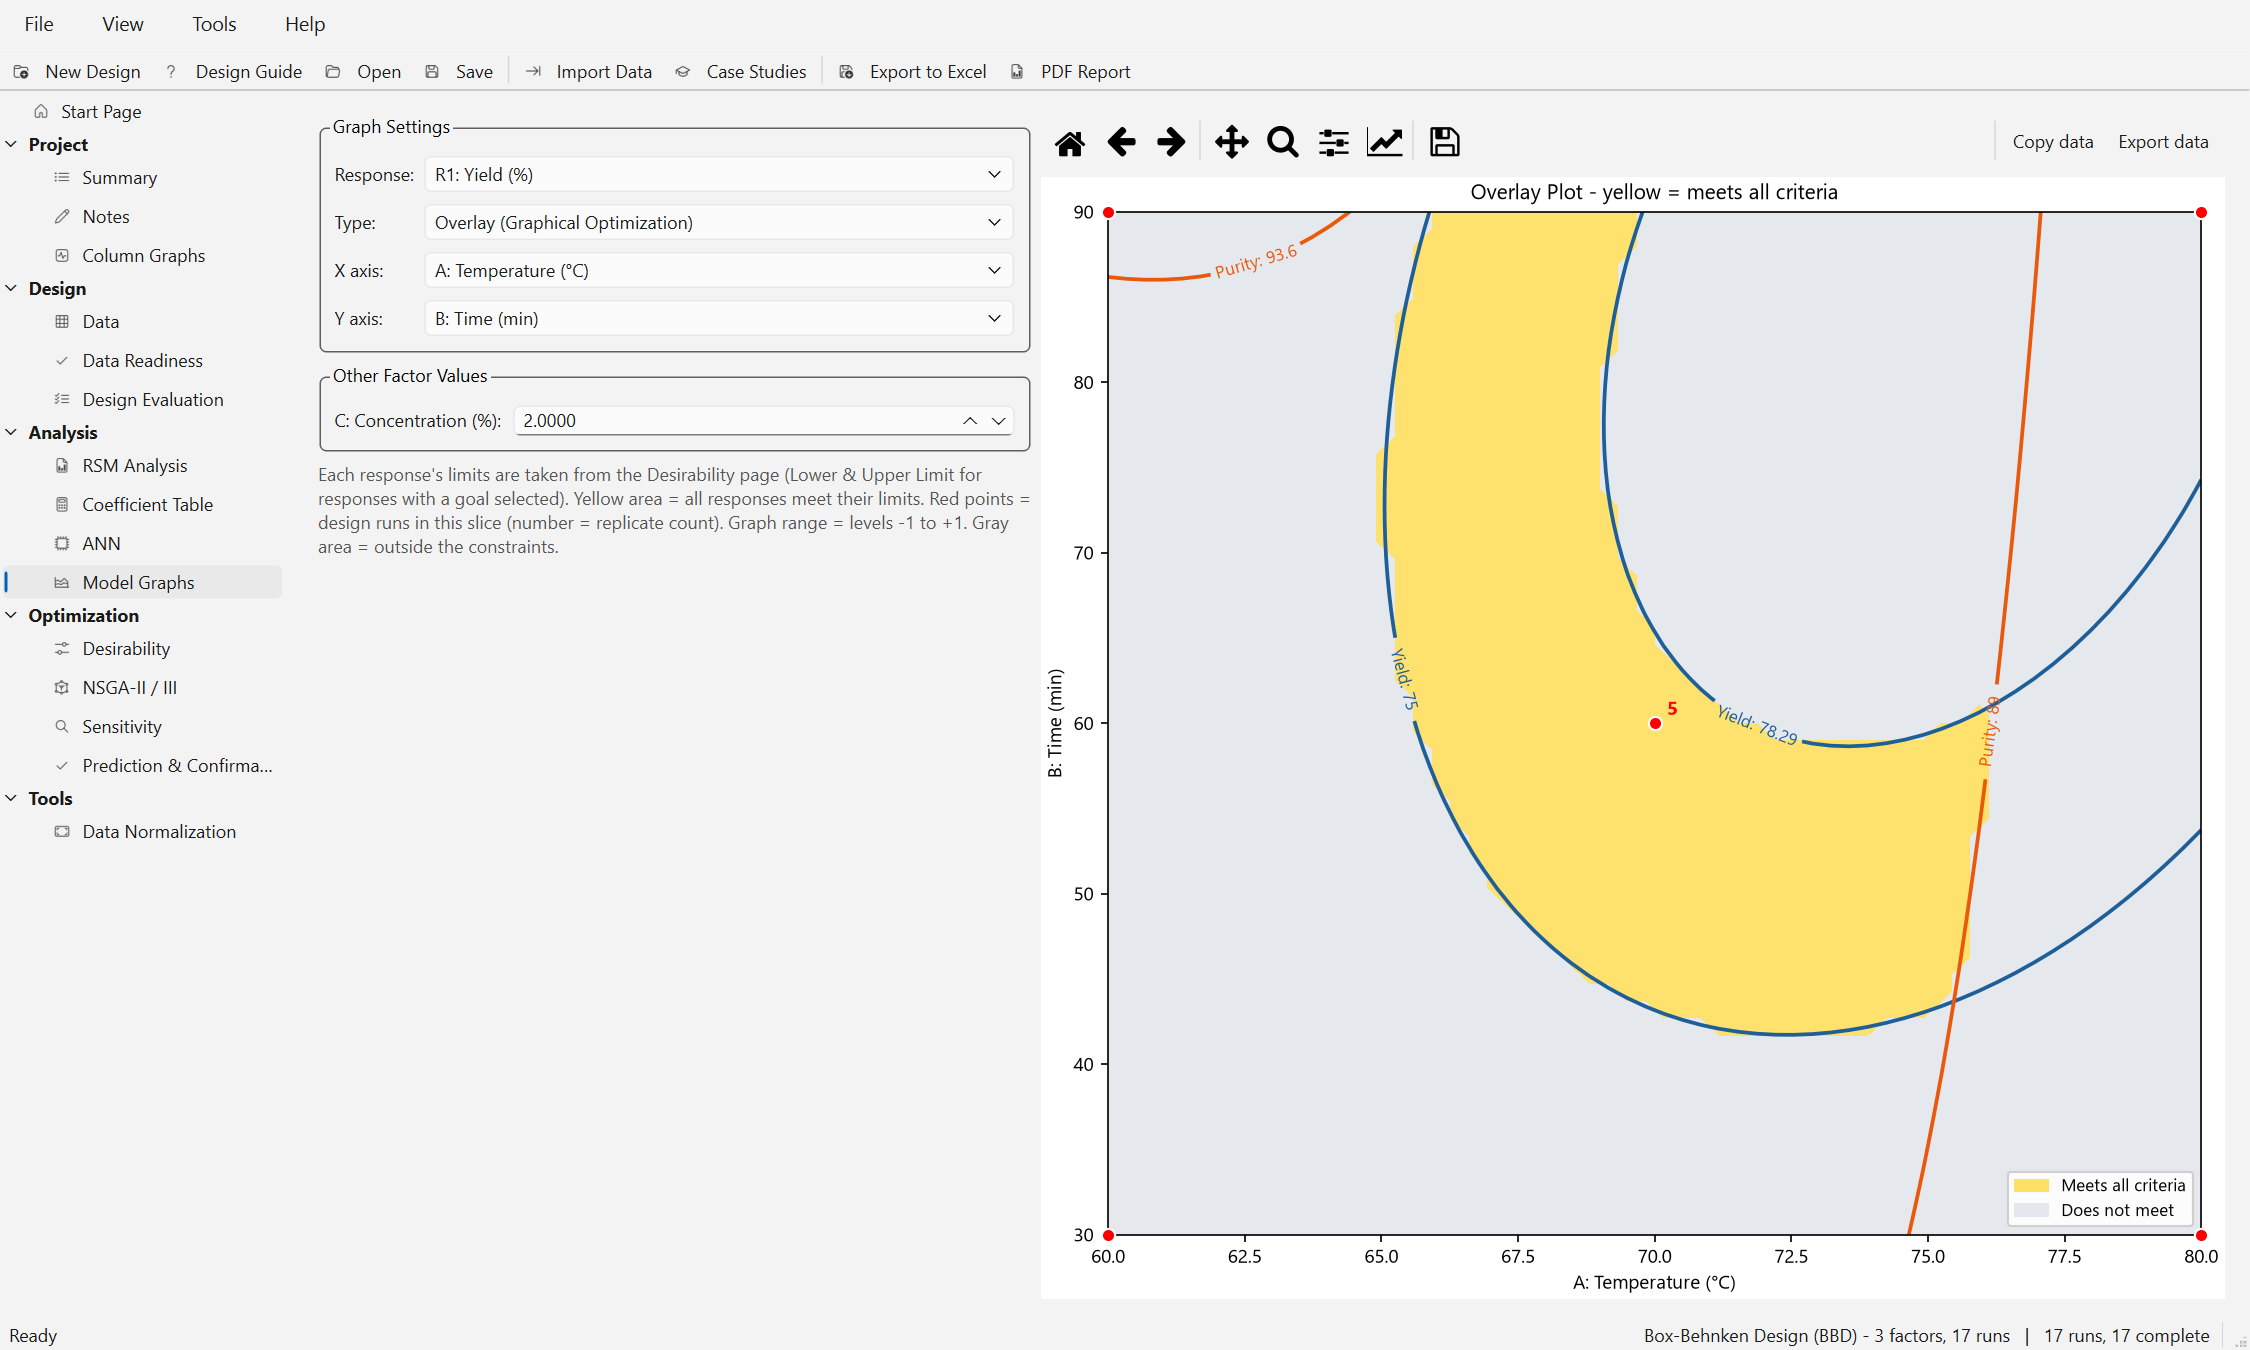
\includegraphics[width=\linewidth]{graph_overlay.png}
\caption{Overlay plot of Yield and Purity; yellow = both responses within their limits.}
\label{fig:ch06-overlay}
\end{figure}

\subsection{Desirability Contour}\label{sec:ch06-desirability}
\paragraph{Purpose.} Shows the combined desirability $D$ of the optimization criteria over the slice, so you
can see how large and how flat the good region is around the numerical optimum.
\paragraph{Theory.} For each response with a goal, the individual desirability \citep{derringer1980} is, with
lower limit $L$, upper limit $H$, target $T$ and shape exponent $s$ (default 1, set on the
\ui{Desirability} page):
\begin{align}
  \text{maximize: }& d=\Big[\text{clip}_{[0,1]}\frac{\hat y-L}{H-L}\Big]^{s},\qquad
  \text{minimize: } d=\Big[\text{clip}_{[0,1]}\frac{H-\hat y}{H-L}\Big]^{s}, \label{eq:ch06-dmax}\\
  \text{target: }& d=\Big(\frac{\hat y-L}{T-L}\Big)^{s}\ (L\le\hat y\le T),\quad
  d=\Big(\frac{H-\hat y}{H-T}\Big)^{s}\ (T<\hat y\le H),\quad d=0\ \text{otherwise}, \label{eq:ch06-dtarget}
\end{align}
and $d=1$ inside $[L,H]$, 0 outside for \emph{In range}. The target defaults to the middle of the limits.
The overall desirability is the importance-weighted geometric mean
\begin{equation}
  D=\exp\Big(\frac{\sum_j r_j\ln d_j}{\sum_j r_j}\Big),\qquad D=0\ \text{if any } d_j=0,
  \label{eq:ch06-D}
\end{equation}
with importance $r_j$ from 1 to 5 (default 3).
\paragraph{Output.} Filled contours of $D$ from 0 to 1 (red to green) with \ui{Contour lines:} levels,
labeled lines, the design points and the optimum star. Note: ``Combined desirability from the criteria on
the Desirability page. Star = latest best solution (if it lies in this slice).''
\paragraph{Example.} In Figure~\ref{fig:ch06-desirability} the best region lies at high Time and
Temperature about 69--72 °C ($D$ up to about 0.83 in this slice). The star is not drawn because the best
solution has Concentration 1.7975\%, not the 2\% of the slice; set Concentration to 1.7975 to see it.

\begin{figure}[htbp]\centering
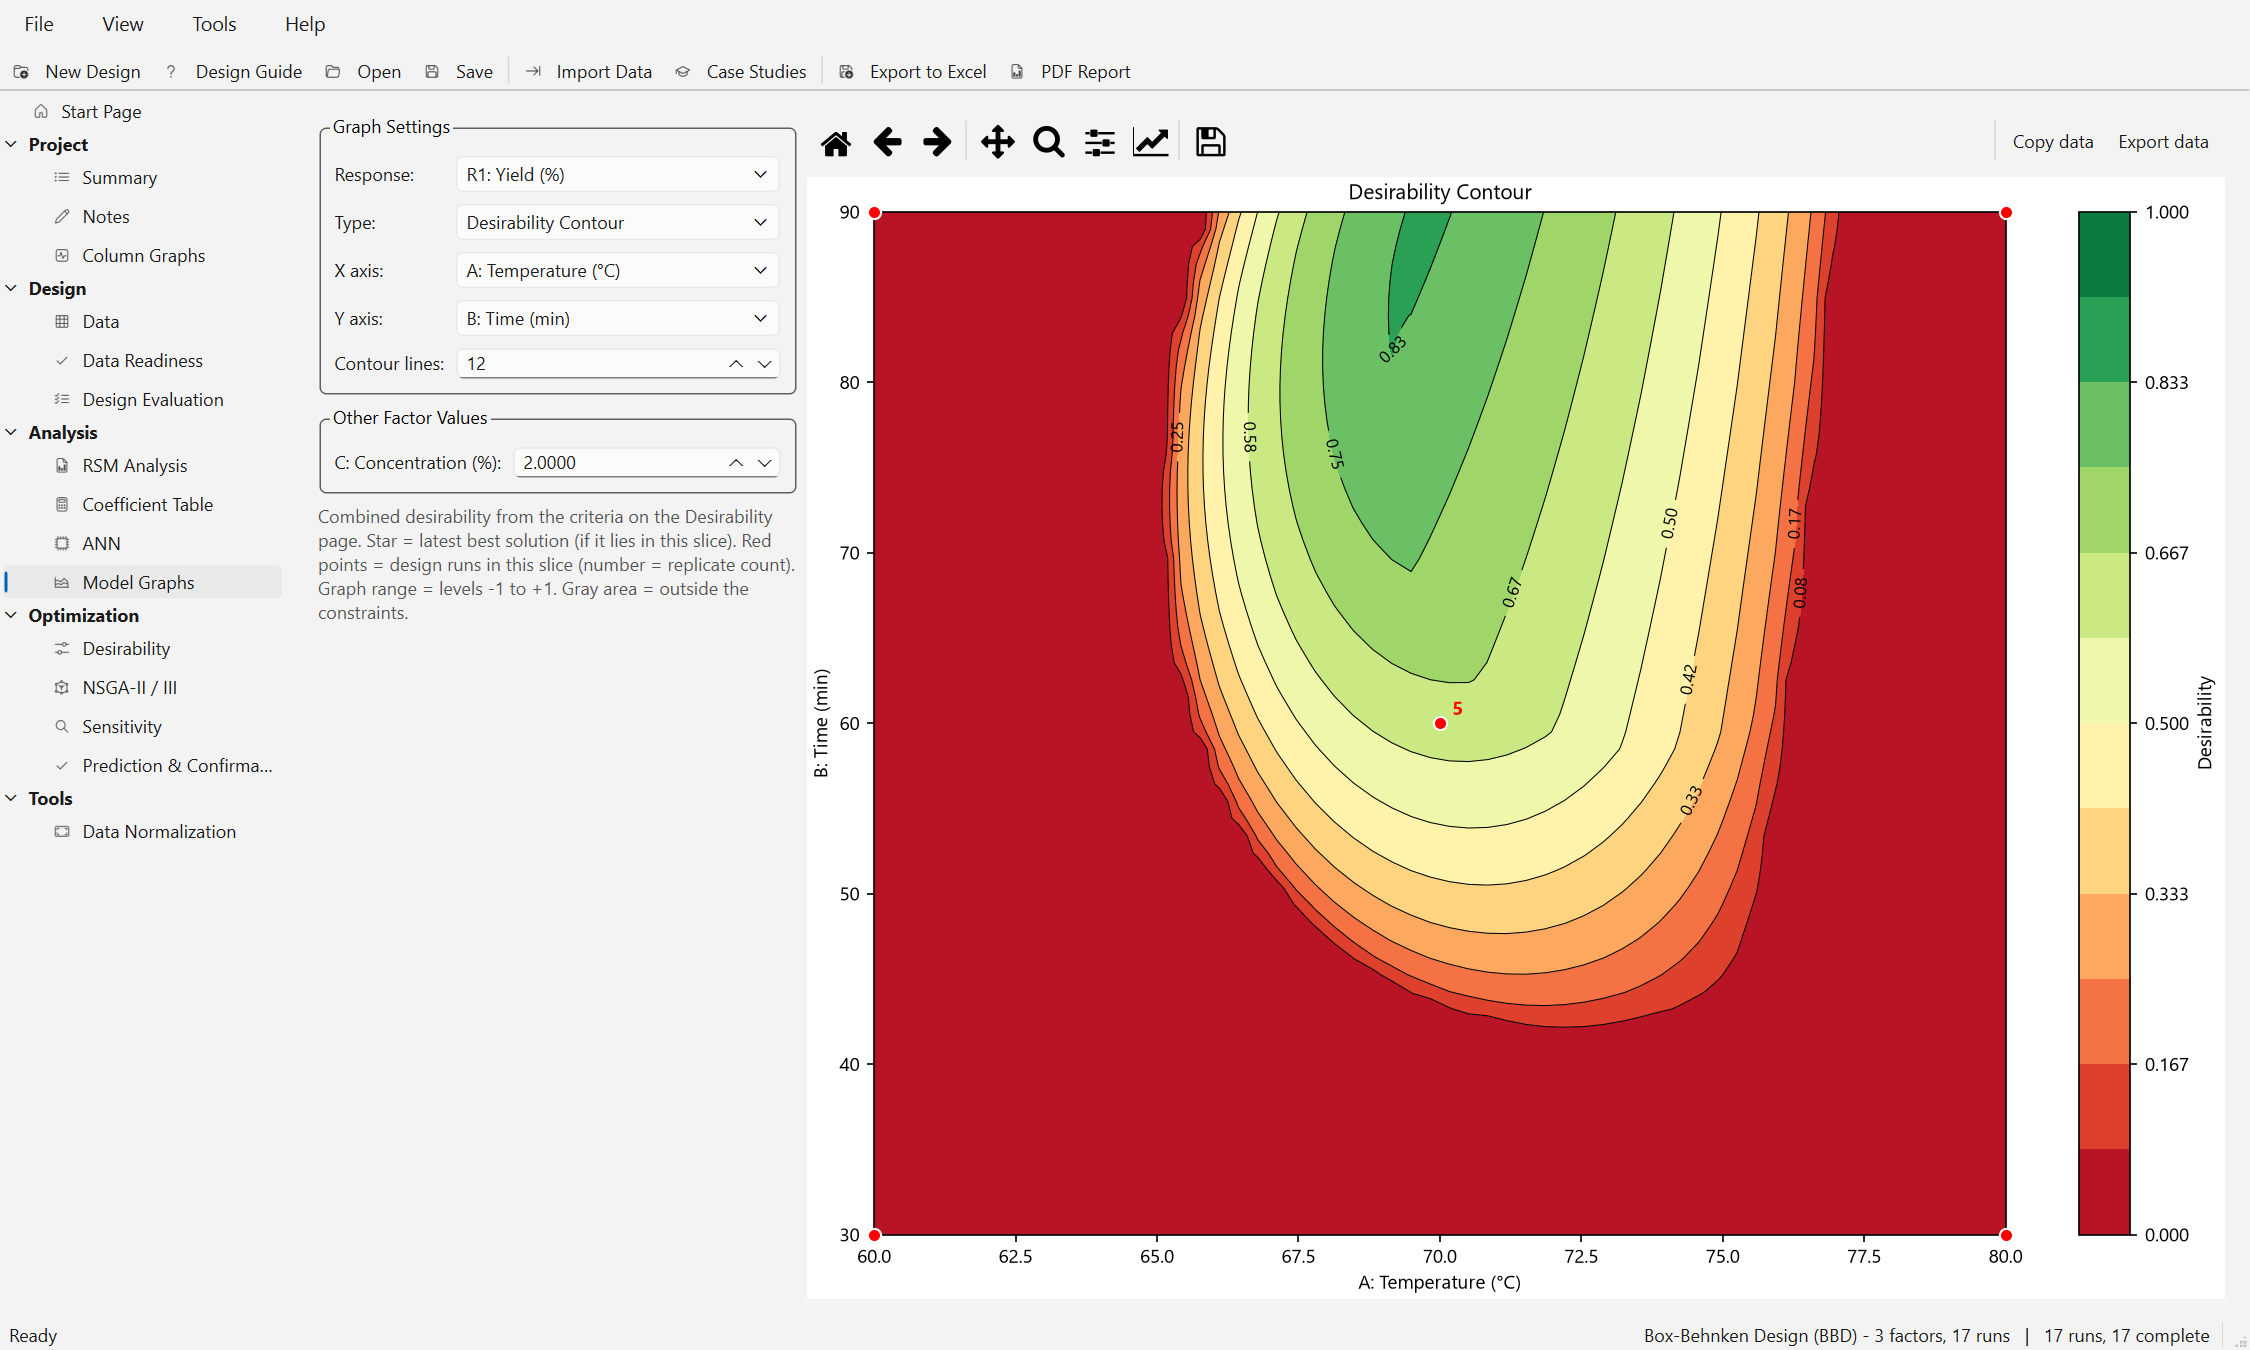
\includegraphics[width=\linewidth]{graph_desirability.png}
\caption{Desirability contour of Yield and Purity (Temperature $\times$ Time, Concentration 2\%).}
\label{fig:ch06-desirability}
\end{figure}

\subsection{Ternary Contour and 3D Ternary Surface}\label{sec:ch06-ternary}
\paragraph{Purpose.} For mixtures the factor space is a simplex; ternary graphs show the response over three
components whose sum is fixed.
\paragraph{How to use.} Choose the components in \ui{Top vertex:}, \ui{Left vertex:} and \ui{Right vertex:}.
With more than three components, or in combined designs, set the other components and the process factors in
\ui{Other Components (Actual Units)}.
\paragraph{Output.} The triangle in pseudo-component space with grid lines for each component labeled in
actual units, filled contours (or a surface), the infeasible area in grey, design points and the optimum
star. Below the triangle: ``Numbers at corners = component amount at the vertex (actual units). Gray area =
outside bounds/constraints.''
\paragraph{Example.} Edible film, Tensile Strength (Figure~\ref{fig:ch06-ternary}): the vertices are Starch
80\%, Glycerol 40\% and Chitosan 40\% (each other component at its lower limit). Strength is highest toward
the Starch-Chitosan edge; the model maximum is about 15.8 MPa at Starch 69.5\%, Glycerol 10\%, Chitosan
20.5\%. Points marked ``2'' are replicated blends.

\begin{figure}[htbp]\centering
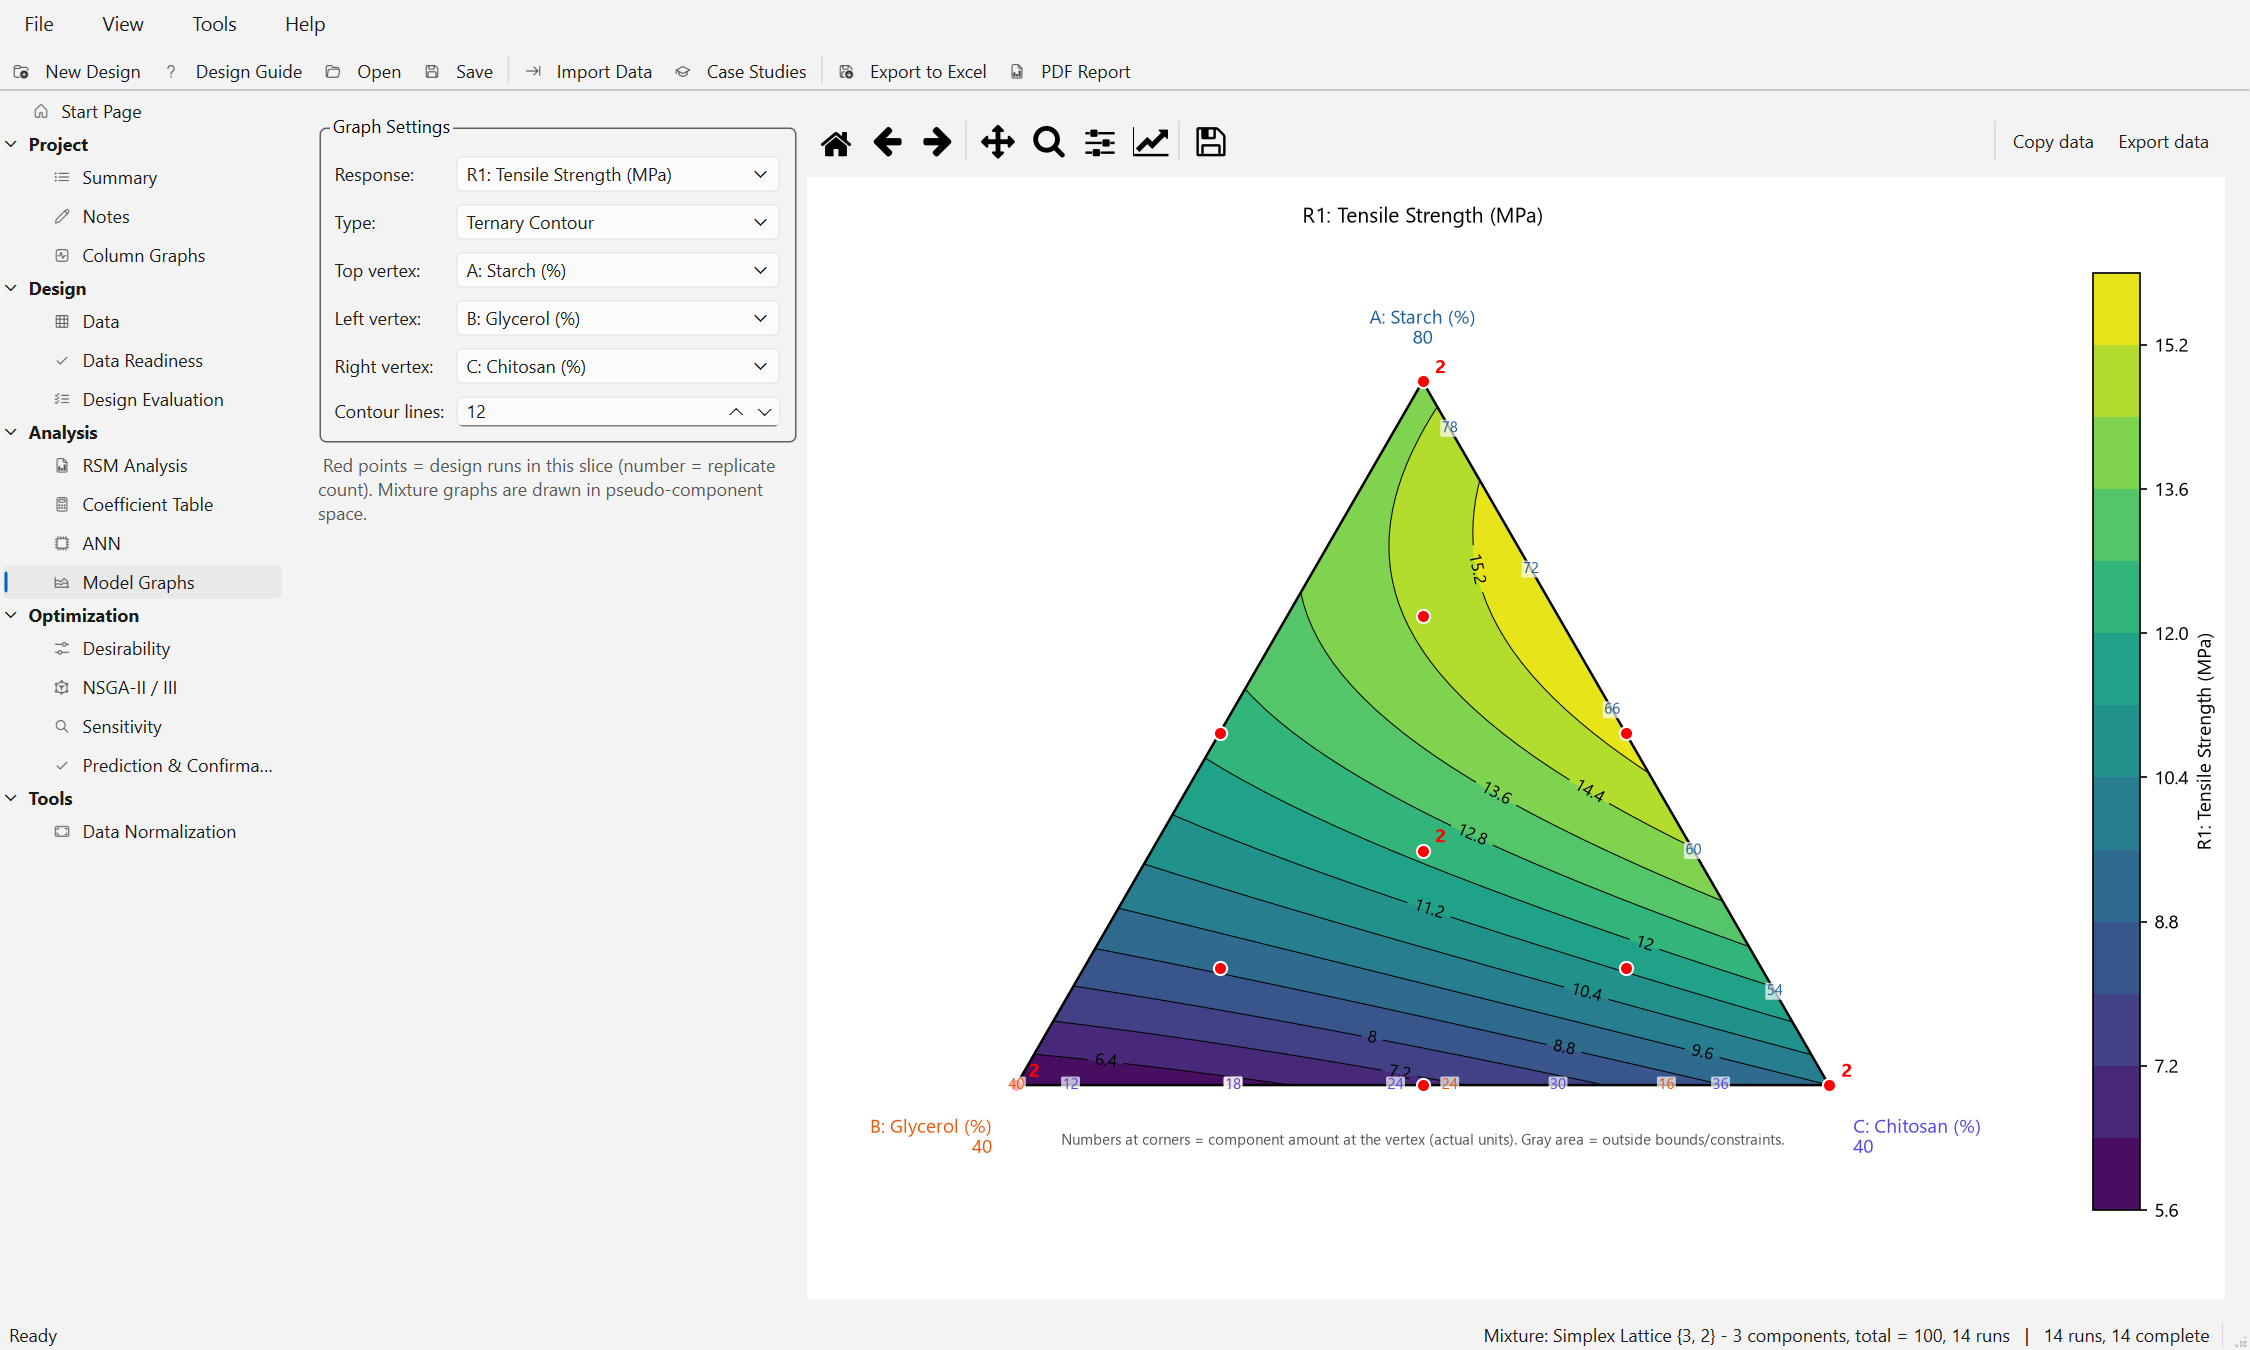
\includegraphics[width=\linewidth]{graph_ternary.png}
\caption{Ternary contour of Tensile Strength (edible film mixture) in pseudo-components.}
\label{fig:ch06-ternary}
\end{figure}

\subsection{Trace (Piepel)}\label{sec:ch06-trace}
\paragraph{Purpose.} The mixture counterpart of the perturbation plot: it shows the effect of each component
when it is increased or decreased from a reference blend while the others keep their relative proportions
\citep{piepel1982,cornell2002}.
\paragraph{Theory.} The reference blend $r$ is the design centroid (mean of the pseudo-component settings).
For component $i$ and $t\in[0,1]$ (201 points)
\begin{equation}
  z_i=t,\qquad z_j=r_j\,\frac{1-t}{1-r_i}\quad(j\neq i),
  \label{eq:ch06-piepel}
\end{equation}
so the sum stays 1 and the ratios between the other components are those of the reference blend
(Piepel's direction). The x-axis is the deviation $t-r_i$ (``Deviation from reference blend
(pseudo-components)''); points outside the bounds or constraints are not drawn. Title ``Trace Plot (Piepel
direction, reference = design centroid)''.
\paragraph{Example.} Edible film, Tensile Strength (Figure~\ref{fig:ch06-trace}), reference blend 60/20/20\%:
increasing Starch raises the strength from 12.2 MPa at the centroid to a maximum of 14.7 MPa at a deviation
of about +0.44; Glycerol lowers it steadily (5.6 MPa at the Glycerol vertex); Chitosan has little effect at
first and lowers it at high amounts.

\begin{figure}[htbp]\centering
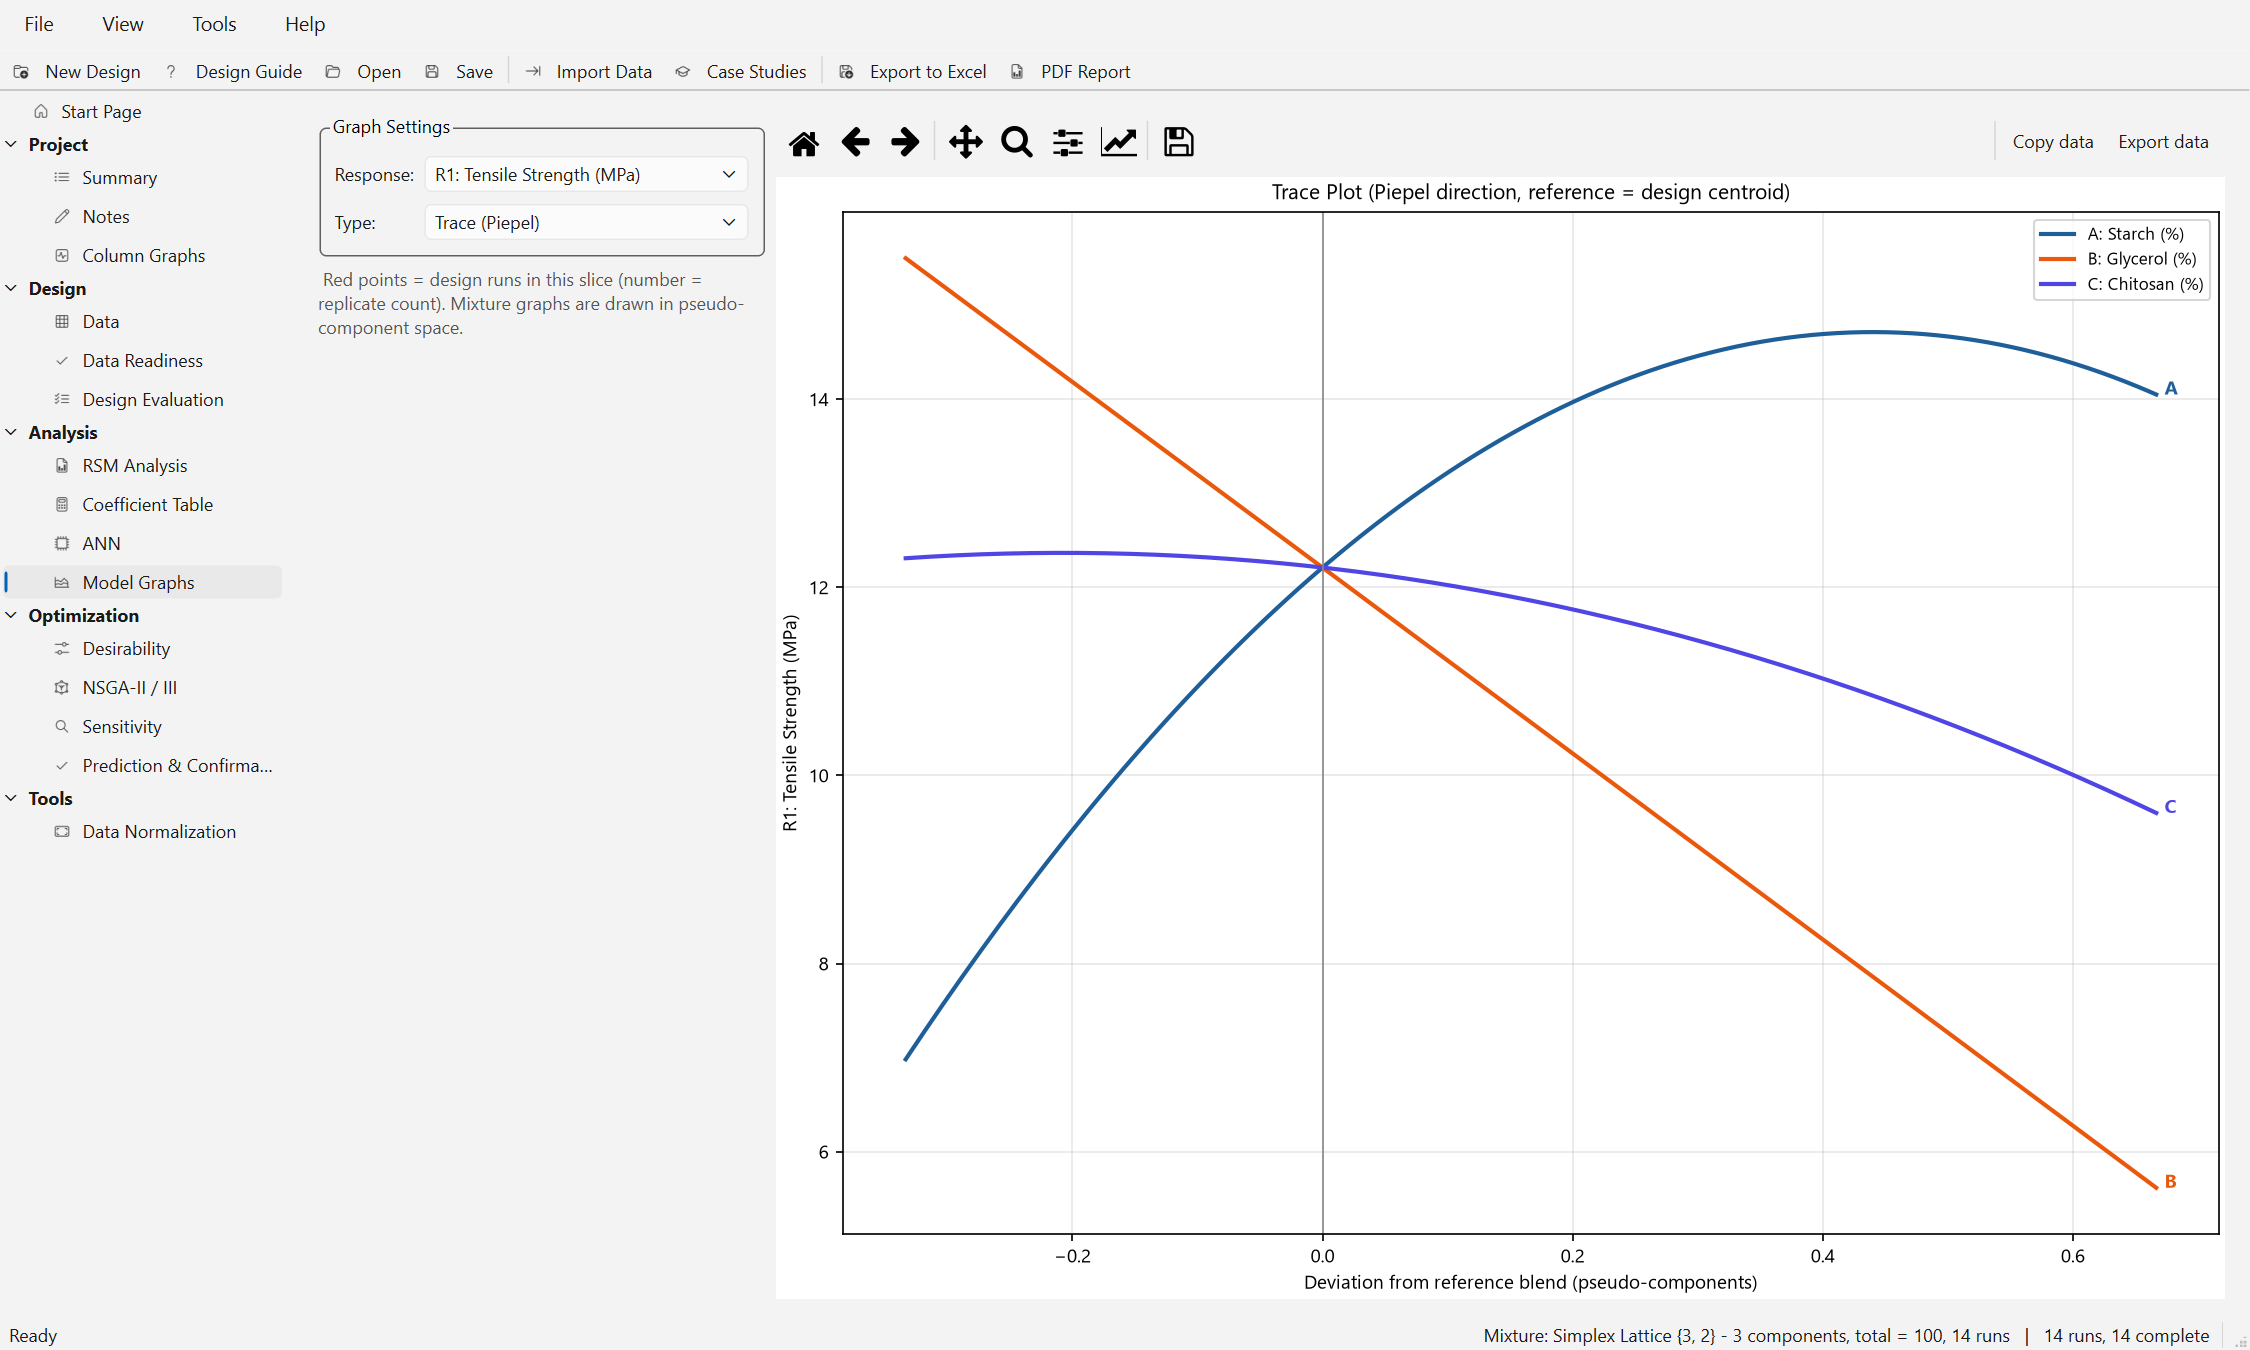
\includegraphics[width=\linewidth]{graph_trace.png}
\caption{Trace plot of Tensile Strength in Piepel's direction from the design centroid.}
\label{fig:ch06-trace}
\end{figure}

\subsection{Propagation of Error (POE)}\label{sec:ch06-poe}
\paragraph{Purpose.} Factors cannot be set exactly in production. POE shows how much variation of the
response is transmitted from the variation of the factors; a robust operating point lies where POE is small.
\paragraph{How to use.} On the \ui{Data} page open \ui{Factor \& Response Info\dots} and enter the standard
deviation $\sigma$ of each factor in actual units (leave it blank for none; not available for categoric
factors). The type \ui{Propagation of Error (POE)} then appears in the \ui{Type:} list. If it is selected
without any $\sigma$, the message ``Enter the factor standard deviations first (Data page $\rightarrow$
Factor \& Response Info...).'' is shown.
\paragraph{Theory as implemented.} With $\sigma_{z,i}$ the standard deviation in coded units
($\sigma_i/h_i$ for a process factor, $\sigma_i/(T-\sum L_j)$ for a mixture component),
\begin{equation}
  \text{POE}(x)=\sqrt{\sum_i\Big(\frac{\partial\hat y}{\partial z_i}\Big)^2\sigma_{z,i}^2
  +\Big(\frac{dg^{-1}(\eta)}{d\eta}\Big)^2\sigma^2_{\text{res}}},
  \label{eq:ch06-poe}
\end{equation}
where the derivatives of the prediction (original units) are central differences with step $10^{-4}$ in
coded units, $g^{-1}$ is the inverse response transformation (its derivative is 1 without a
transformation) and $\sigma^2_{\text{res}}$ is the residual variance: MSE for least squares,
$\hat\sigma^2+\hat\sigma^2_{wp}$ for split-plot models, the mean squared error for an ANN and 0 for GLM
responses. The first term is the variation transmitted by the factors (first-order Taylor expansion, factor
errors assumed independent); the second is the variation that remains even when the factors are set exactly,
so POE is never below $\sigma_{\text{res}}$ for an untransformed response. Mixture components are perturbed
one at a time without renormalizing the blend. The POE graph is a contour plot like
Section~\ref{sec:ch06-contour}, with the title listing the $\sigma$ values.
\paragraph{Example.} Box-Behnken case with $\sigma$ = 1.0 °C, 2.0 min and 0.05\% (Figure~\ref{fig:ch06-poe});
in coded units 0.10, 0.067 and 0.05. In the slice at 2\% Concentration POE ranges from 0.72 to 1.86\%; it is
0.85 at the center. The smallest value, 0.72, lies at about 75 °C and 85 min, close to
$\sqrt{\text{MSE}}=0.714$: there the slope of the surface is almost zero, because this point is the
maximum of Yield in the slice. Here the most productive and the most robust settings coincide.

\begin{figure}[htbp]\centering
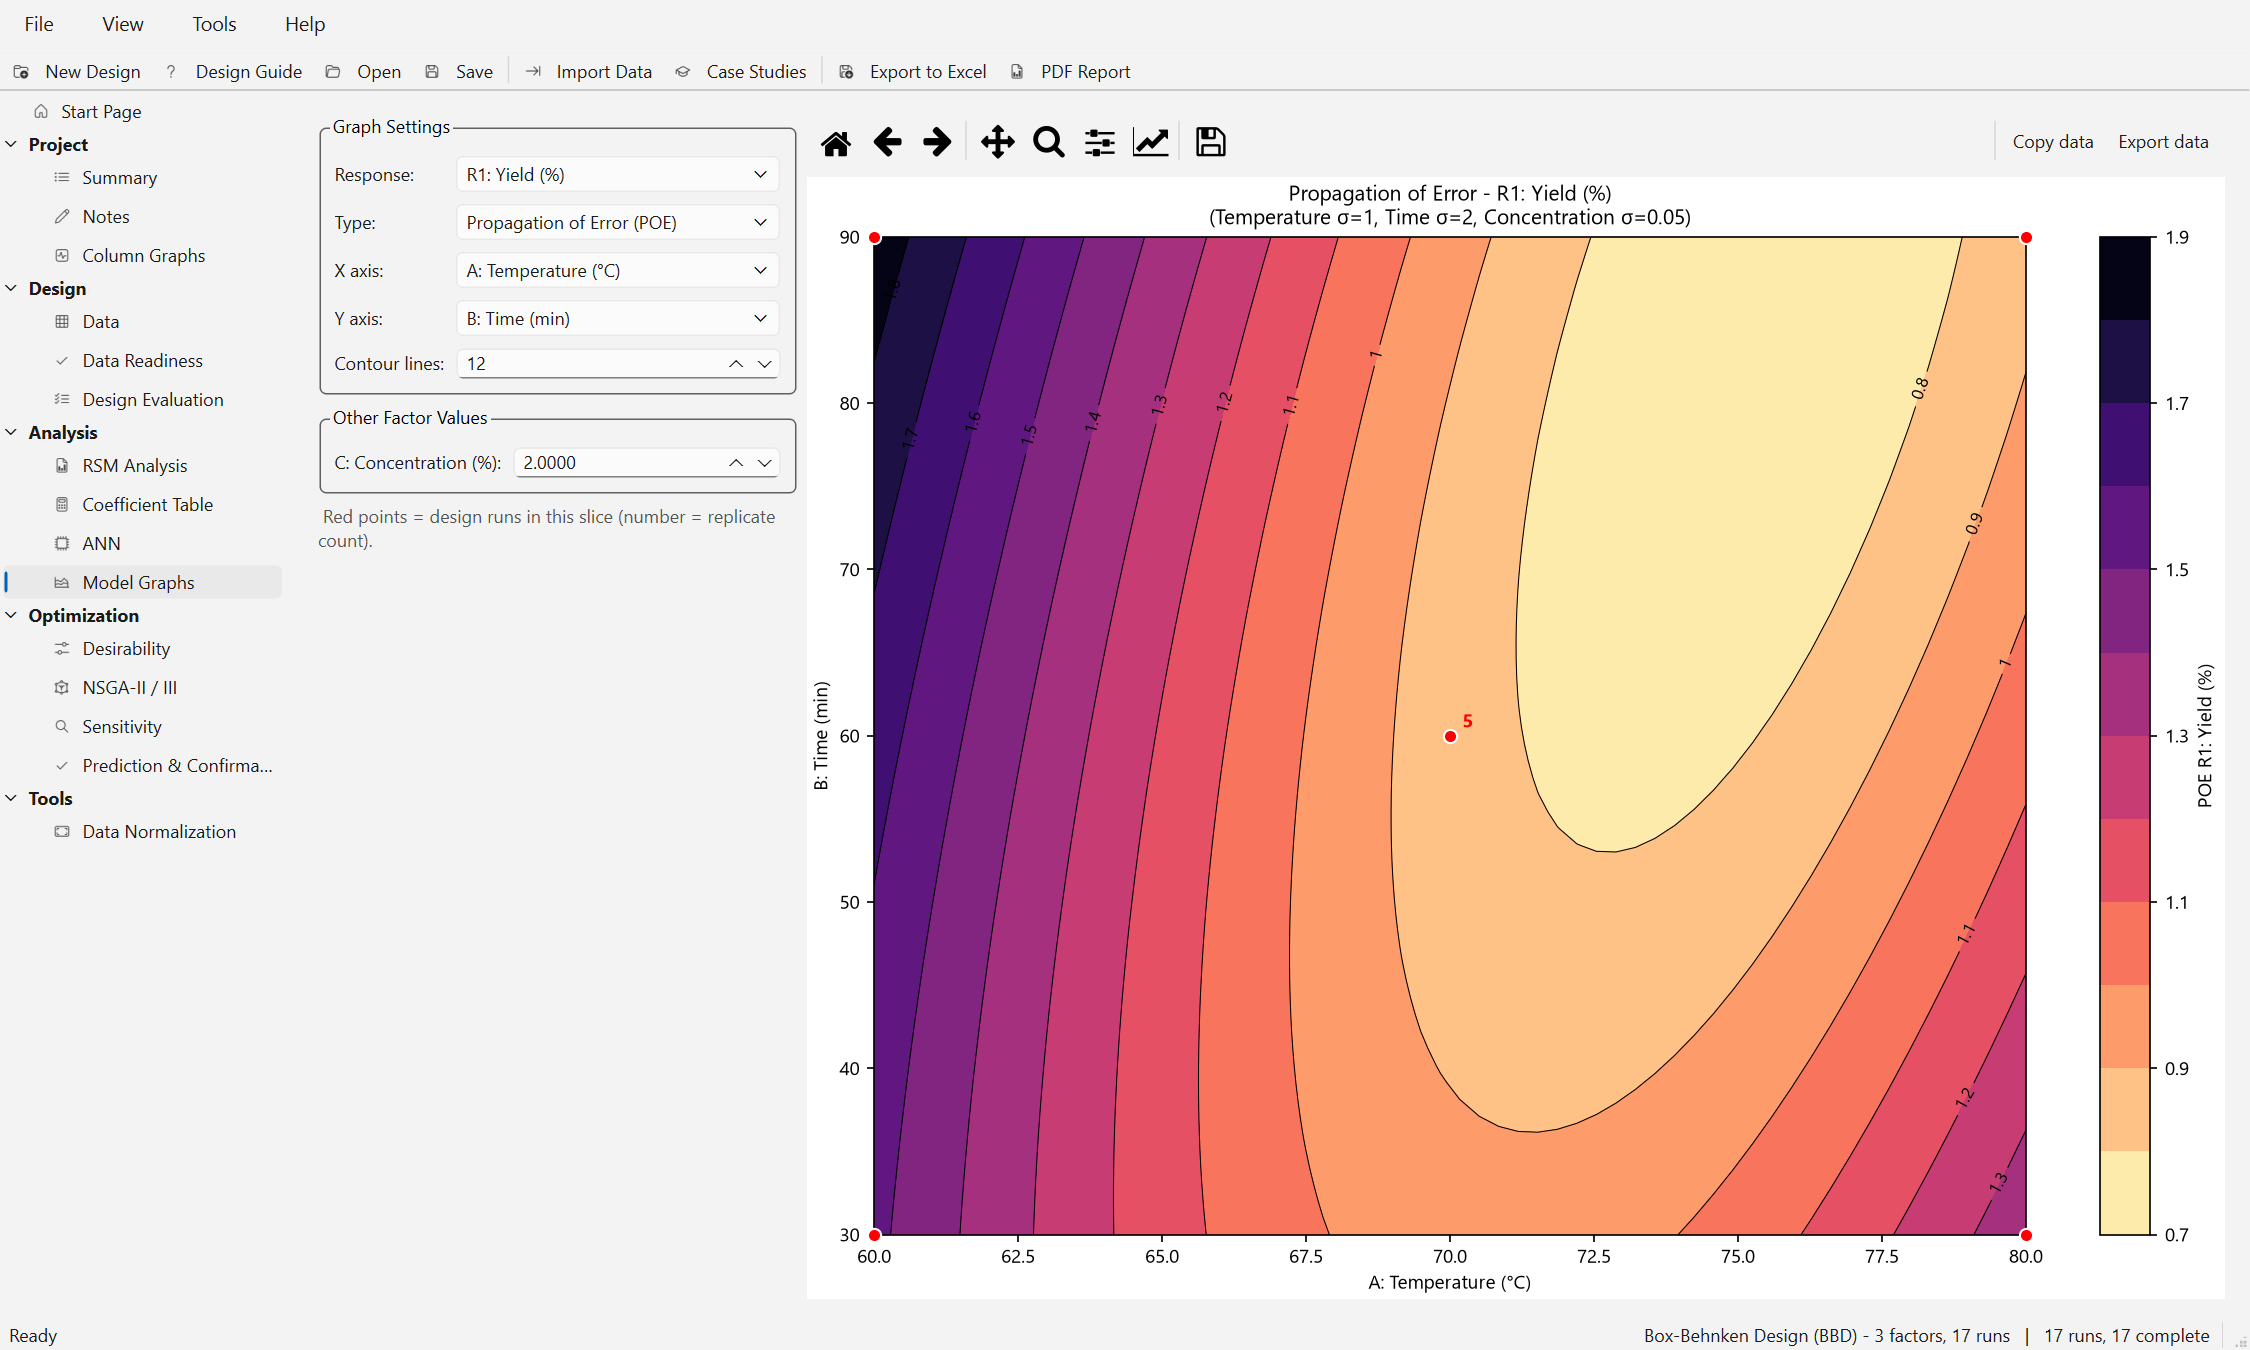
\includegraphics[width=\linewidth]{graph_poe.png}
\caption{Propagation of error of Yield for factor standard deviations of 1.0 °C, 2.0 min and 0.05\%.}
\label{fig:ch06-poe}
\end{figure}

\section{Exporting the data behind a graph}\label{sec:ch06-export}

Every graph can be saved as an image with the toolbar button for saving, and the data behind it can be
reused elsewhere (Figure~\ref{fig:ch06-toolbar}):
\begin{itemize}
  \item \ui{Copy data} (toolbar) or \ui{Copy plot data} (right-click on the plot) puts the data on the
        clipboard, ready to paste into a spreadsheet;
  \item \ui{Export data\dots} (toolbar) or \ui{Export plot data\dots} (right-click) writes an Excel
        workbook with one sheet per data series, or a CSV file with the tables below each other.
\end{itemize}

\begin{figure}[htbp]\centering
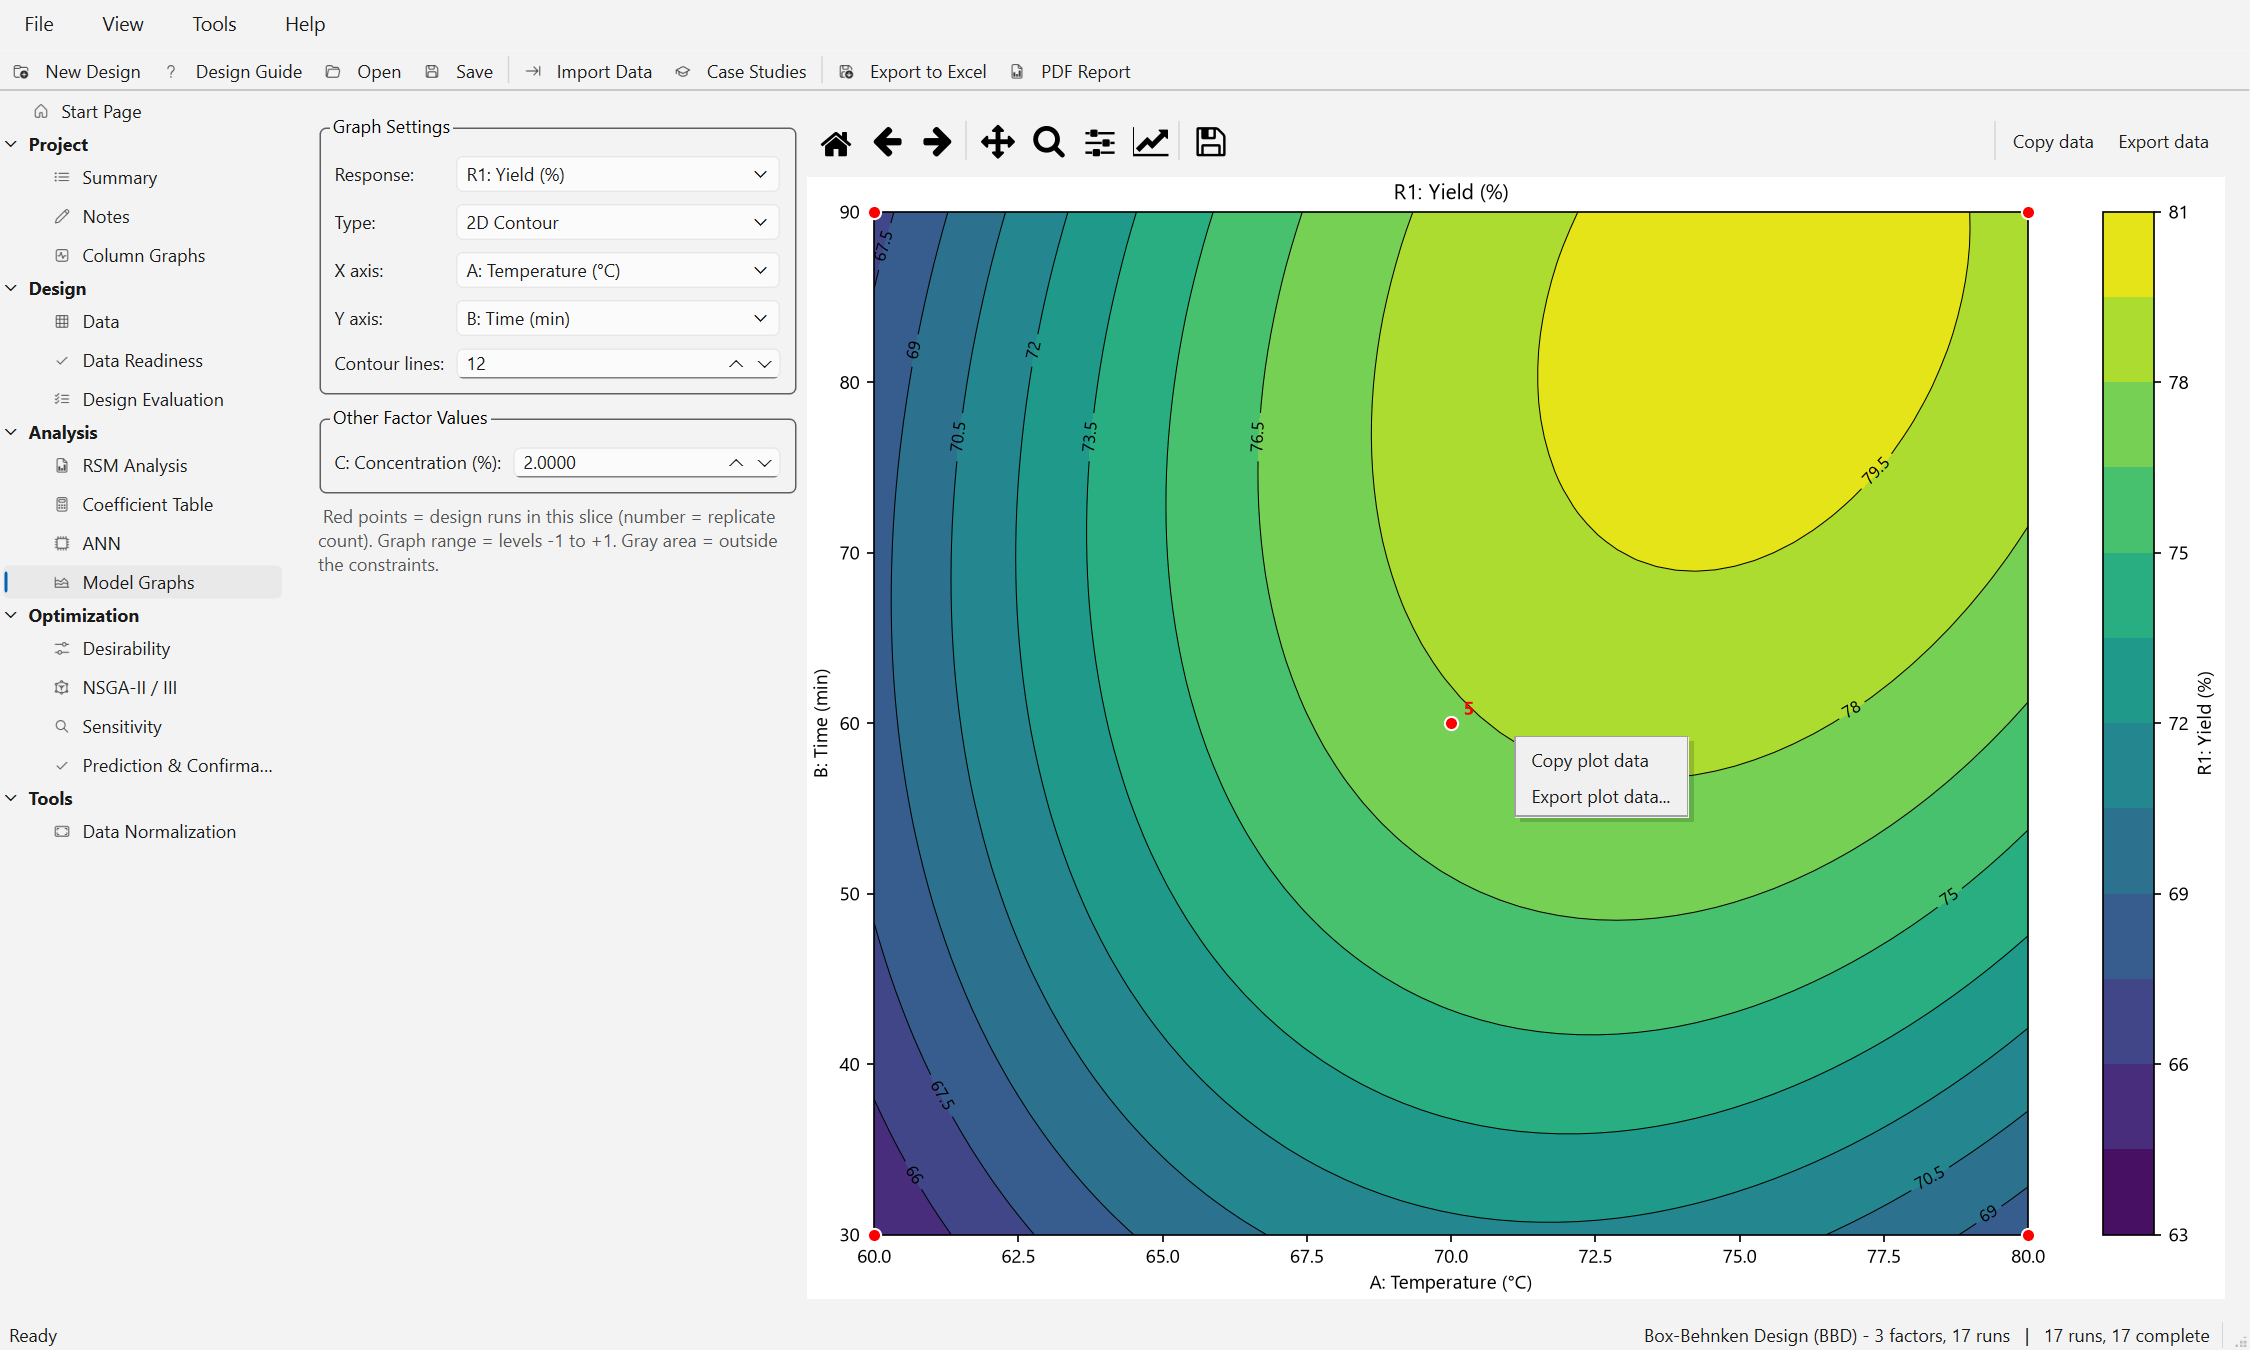
\includegraphics[width=0.75\linewidth]{plot_context_menu.png}
\caption{Right-click menu of a graph with \ui{Copy plot data} and \ui{Export plot data\dots}.}
\label{fig:ch06-toolbar}
\end{figure}

What is exported depends on the graph:
\begin{itemize}
  \item \emph{2D Contour, 3D Surface, ternary graphs, POE}: the full grid. One row per grid point with the
        axis factors in actual units, the column \ui{Inside region (1 = yes)} and the plotted value (the
        response, or \ui{POE} followed by the response name). The table title lists the values of the other
        factors of the slice.
  \item \emph{Overlay}: the grid with the predicted value of each response (column name with its limits)
        and \ui{Meets all criteria (1 = yes)}.
  \item \emph{Desirability Contour}: the grid with the column \ui{Desirability}.
  \item \emph{Design points}: a table ``Design points in this slice'' with the factor values and
        \ui{Number of runs} (3D surfaces: the observed responses); the optimum star, when drawn, as its own
        table.
  \item \emph{One Factor Effect, All Factors}: the predicted line and the 95\% confidence interval
        (columns \ui{Lower} and \ui{Upper}); for categoric factors the points with their error bars.
  \item \emph{Interaction, Perturbation, Trace}: the plotted lines and error bars as drawn.
  \item \emph{Cube Plot}: the table ``Cube corners'' with the eight corners in actual units and the
        predicted response at each corner (the title lists the values of the other factors, if any).
\end{itemize}
To redraw a contour plot in another program, use the grid table, keep the rows with
\ui{Inside region (1 = yes)} equal to 1 and reshape the values to the $60\times60$ grid (process designs).

% Chapter 7: Artificial Neural Networks
\chapter{Artificial Neural Networks}\label{sec:ch07-ann}\label{chap:7}

A response surface model is a low-order polynomial. It works very well when the response is smooth over the
region studied, but it cannot follow sharp optima, saturation, plateaus or strong interactions of more than two
factors. An artificial neural network (ANN) is a flexible nonlinear regression model that can follow such
patterns, provided there are enough runs to estimate it and to check it on data it has not seen. The
\ui{ANN} page (navigation group \ui{Analysis}, page title \ui{Artificial Neural Network}) fits multilayer
perceptrons to the continuous responses of the project and answers four questions:
\begin{enumerate}
  \item Are the data adequate for an ANN at all (\ui{Data Adequacy})?
  \item Which network size is supported by the data (check~A, the cross-validated architecture search)?
  \item Does the fitted network generalize, or does it underfit or overfit (\ui{Fit Diagnosis})?
  \item Would more runs still improve the network, and roughly how many (check~B, the learning curve)?
\end{enumerate}
A network trained here can replace the RSM model of the same response in the model graphs, in the desirability and
NSGA optimizations, in the sensitivity study and on the \ui{Prediction \& Confirmation} page
(Section~\ref{sec:ch07-use}). Binomial and Poisson responses are not modeled with an ANN; they are analyzed with
logistic or Poisson regression on the \ui{RSM Analysis} page.

The examples in this chapter use the case study \ui{Dye Adsorption (ANN, 40 runs)} (\menupath{File $\rightarrow$
Case Studies\dots}). It contains 40 historical runs placed by a Latin hypercube in four factors (A: pH 2--10,
B: Adsorbent Dose 0.5--4~g/L, C: Contact Time 10--120~min, D: Initial Concentration 20--200~mg/L) and one
response, R1: Removal Efficiency (\%), which ranges from 2.73 to 58.45~\%. The response has a pH optimum, a
kinetic and an isotherm effect, so it is strongly nonlinear. All numbers below were obtained with the default
settings, random seed 1 and one CPU core; the screenshots show the same state.

\section{Layout of the page and suggested workflow}\label{sec:ch07-layout}

The page has a scrollable control panel on the left and ten result tabs on the right
(Figure~\ref{fig:ch07-summary}). At the top of the left panel, \ui{Show response:} selects the response whose
results are shown. Changing it re-runs the data adequacy assessment and refreshes all tabs. Below it are four
groups:
\begin{itemize}
  \item \ui{1. Data Adequacy}: the verdict, the buttons \ui{Assess Data Adequacy} and
    \ui{Learning Curve (Enough Data?)} (check~B).
  \item \ui{2. ANN Model}: one network per response or one network for several responses.
  \item \ui{3. Network Settings}: algorithm, normalization, activation, early stopping, network size, data
    split, restarts, epochs, seed, CPU cores and the button \ui{Train ANN (This Response)}.
  \item \ui{4. Optimize Layers \& Neurons (Automatic)}: the settings of the architecture search (check~A) and the
    buttons \ui{Search Architecture (This Response)} and \ui{Optimize All Responses (One Click)}.
\end{itemize}
Under the groups are a status line, the check box \ui{Use this response's ANN for graphs, optimization, NSGA-II \&
prediction} and a reminder of the suggested workflow:
\begin{enumerate}
  \item Fit the RSM model of the response first on the \ui{RSM Analysis} page. The ANN page uses the current RSM
    model as the reference in every comparison.
  \item Read the \ui{Data Adequacy} report (it is produced automatically when the page opens).
  \item Click \ui{Optimize All Responses (One Click)} or \ui{Search Architecture (This Response)}. The application
    chooses the number of hidden layers and neurons by cross-validation and trains the final network.
  \item Read the \ui{Fit Diagnosis} on the \ui{Summary \& Diagnosis} tab and compare with RSM on the
    \ui{Architecture Search} tab.
  \item If the data are borderline, run \ui{Learning Curve (Enough Data?)}.
  \item Tick \ui{Use this response's ANN for graphs, optimization, NSGA-II \& prediction} only if the ANN
    predicts new data better than the RSM model.
\end{enumerate}

Table~\ref{tab:ch07-tabs} lists the result tabs. While a model is missing, the plot tabs show ``No ANN model yet''
and the \ui{Summary \& Diagnosis} tab explains how to train one.

\begin{table}[htbp]
\centering
\caption{Result tabs of the ANN page.}\label{tab:ch07-tabs}
\begin{tabularx}{\linewidth}{@{}lX@{}}
\toprule
Tab & Content \\
\midrule
\ui{Data Adequacy} & Report of the eleven adequacy checks, verdict, recommendations; response histogram and check
  summary (Section~\ref{sec:ch07-adequacy}). \\
\ui{Learning Curve} & Check~B: test $R^2$ against the number of training runs, power-law fit, estimate of the runs
  needed (Section~\ref{sec:ch07-learning}). \\
\ui{Summary \& Diagnosis} & Architecture, algorithm, data split, fit diagnosis, performance table, RSM comparison,
  factor importance (Section~\ref{sec:ch07-diagnosis}). \\
\ui{Architecture Search} & Check~A: all candidate networks, best per depth, selected network, comparison with
  RSM on the same test data (Section~\ref{sec:ch07-search}). \\
\ui{Regression Plots} & Output against target for training, validation, test and all data. \\
\ui{Training Performance} & Error per epoch for training, validation and test data. \\
\ui{Factor Importance} & Relative importance of each factor by Garson's method. \\
\ui{RSM vs ANN} & Predicted against actual values and residuals per run for both models. \\
\ui{Network Diagram} & Nodes and connections, colored by the sign of the weight. \\
\ui{Weights \& Biases} & All weights, biases and normalization parameters. \\
\bottomrule
\end{tabularx}
\end{table}

\section{The network model}\label{sec:ch07-model}

\subsection{Structure}

REGEN uses a fully connected feed-forward network (multilayer perceptron) with $L \ge 1$ hidden layers of
$h_1,\dots,h_L$ neurons and a linear output layer with $n_\text{out}$ outputs. There is no upper limit on the
number of layers or neurons. With the normalized input vector $\mathbf{x}_n$,
\begin{align}
  \mathbf{h}^{(0)} &= \mathbf{x}_n, \label{eq:ch07-input}\\
  \mathbf{h}^{(l)} &= f\!\left(\mathbf{W}^{(l)}\mathbf{h}^{(l-1)} + \mathbf{b}^{(l)}\right),
     \qquad l = 1,\dots,L, \label{eq:ch07-hidden}\\
  \mathbf{y}_n &= \mathbf{W}_\text{out}\,\mathbf{h}^{(L)} + \mathbf{b}_\text{out}, \label{eq:ch07-output}
\end{align}
where $\mathbf{W}^{(l)}$ ($h_l \times h_{l-1}$) and $\mathbf{b}^{(l)}$ are the weights and biases of layer $l$ and
$\mathbf{y}_n$ is the normalized output. The activation function of the hidden neurons is selected with
\ui{Activation function:}:
\begin{equation}
  \text{tansig: } f(a) = \tanh a, \qquad \text{logsig: } f(a) = \frac{1}{1+e^{-a}}. \label{eq:ch07-act}
\end{equation}
The default and recommended choice is \ui{tansig (tanh)}, which is centered on zero and matches the input range
$[-1,1]$ of the default normalization. The output layer is always linear, so the network can predict any value
of the response and is not limited to the range of the activation function.

The number of adjustable parameters (weights and biases) is
\begin{equation}
  W = \sum_{l=1}^{L} h_l\,(h_{l-1}+1) + n_\text{out}\,(h_L+1), \qquad h_0 = n_\text{in}.
  \label{eq:ch07-nweights}
\end{equation}
The network is written as the string $n_\text{in}$-$h_1$-$\cdots$-$h_L$-$n_\text{out}$. For the dye case
with one hidden layer of 3 neurons, the network is 4-3-1 with $W = 3\cdot 5 + 1\cdot 4 = 19$ weights. Below the
entry \ui{Neurons per hidden layer:} the page shows the number of layers and of weights for the current entry,
for example ``1 hidden layer, 19 weights''.

\subsection{Inputs, outputs and normalization}\label{sec:ch07-norm}

The network inputs are the factors in coded units: $-1$ to $+1$ for process factors and pseudo-components for
mixture components. A categorical factor with $m$ levels becomes $m$ one-hot input columns (one column per level,
1 for the level of the run and 0 otherwise), so $n_\text{in}$ counts these columns. The responses enter in their
original units. The response transformation chosen on the \ui{RSM Analysis} page is \emph{not} used by the ANN.

Before training, every input column and every output is normalized by
\begin{equation}
  x_n = \text{base} + \frac{x - \text{offset}}{\text{scale}}, \qquad
  y = (y_n - \text{base})\cdot\text{scale} + \text{offset}, \label{eq:ch07-normalize}
\end{equation}
where the second relation converts the network output back to response units. The parameters depend on the option
\ui{Normalization:} (Table~\ref{tab:ch07-norm}). They are computed from the \emph{training and validation} runs
only; the test runs never influence them, so no information leaks from the test data into the model. A scale of
zero (a constant column) is replaced by 1. A response that is constant over the training and validation runs
cannot be modeled (message ``Constant response - the ANN cannot be trained.'').

\begin{table}[htbp]
\centering
\caption{Normalization options (\ui{Normalization:}); min, max, mean and SD are computed per column over the
training and validation runs.}\label{tab:ch07-norm}
\begin{tabularx}{\linewidth}{@{}Xllll@{}}
\toprule
Option & offset & scale & base & Range of $x_n$ \\
\midrule
\ui{Min-max to [-1, 1] (mapminmax) - recommended} (default) & min & (max $-$ min)/2 & $-1$ & $[-1,1]$ \\
\ui{Min-max to [0, 1]} & min & max $-$ min & 0 & $[0,1]$ \\
\ui{Z-score standardization (mapstd): mean 0, SD 1} & mean & SD & 0 & mean 0, SD 1 \\
\ui{No normalization (for comparison)} & 0 & 1 & 0 & unchanged \\
\bottomrule
\end{tabularx}
\end{table}

Normalization matters because the inputs and outputs have very different ranges. In the dye case the largest
range (Initial Concentration, 180~mg/L) is 51 times the smallest (Adsorbent Dose, 3.5~g/L). Without normalization
the large variables dominate the error and the gradients, and the tanh neurons saturate. The option \ui{No
normalization (for comparison)} exists only to demonstrate this. The same transformations can be inspected on
the \ui{Data Normalization} page (navigation group \ui{Tools}).

\subsection{Separate and combined networks}\label{sec:ch07-combined}

Group \ui{2. ANN Model} offers two options:
\begin{itemize}
  \item \ui{Separate - one network per response} (default): each response gets its own network and its own
    architecture. This is usually more accurate.
  \item \ui{Combined - one network for several responses}: one multi-output network models all responses checked
    in the list \ui{Responses combined in one network:}. Non-continuous responses are listed with the suffix
    ``(not continuous)'' and cannot be checked; at least two continuous responses are needed. The buttons change
    to \ui{Train Combined ANN} and \ui{Search Architecture (Combined Model)}, and \ui{Optimize All Responses (One
    Click)} is hidden.
\end{itemize}
In a combined network the hidden layers are shared and the output layer has one linear neuron per response. The
training error sums over all outputs, the normalized errors are averaged over the outputs, and the plots of a
response show its own output. A combined model is more compact and can be useful when the responses are
physically related, but every response then has to accept the same hidden layers. Training a new network for a
response that belongs to a combined network breaks the old combined network apart.

\section{Network settings and training}\label{sec:ch07-training}

\subsection{How to train a network by hand}

\begin{enumerate}
  \item Select the response in \ui{Show response:}.
  \item In \ui{3. Network Settings}, choose the algorithm, normalization and activation, and type the neurons per
    hidden layer, for example \texttt{5} (one layer), \texttt{8, 4} (two layers) or \texttt{64, 32, 16, 8}.
    Commas, semicolons or spaces separate the layers.
  \item Check the data split and the other settings (Table~\ref{tab:ch07-settings}).
  \item Click \ui{Train ANN (This Response)}. The progress line shows ``Training \dots: restart $i$/$n$'' and the
    \ui{Stop} button interrupts the work. When training is finished the status line reads, for example, ``Done:
    4-3-1, Overfitting'' and the \ui{Summary \& Diagnosis} tab opens.
\end{enumerate}
Setting the network size by hand is useful for teaching and for comparisons. For a model that will be used,
let the architecture search choose the size (Section~\ref{sec:ch07-search}).

\begin{table}[htbp]
\centering
\caption{Options of group \ui{3. Network Settings}.}\label{tab:ch07-settings}
\begin{tabularx}{\linewidth}{@{}>{\raggedright\arraybackslash}p{3.3cm}>{\raggedright\arraybackslash}p{3.2cm}>{\raggedright\arraybackslash}p{2.15cm}X@{}}
\toprule
Option & Values & Default & Meaning \\
\midrule
\ui{Algorithm:} & \ui{Bayesian Regularization (trainbr)}, \ui{Levenberg-Marquardt (trainlm)}, \ui{Adam mini-batch}
  & trainbr & Training algorithm (Section~\ref{sec:ch07-algorithms}). \\
\ui{Normalization:} & four options & mapminmax & Table~\ref{tab:ch07-norm}. \\
\ui{Activation function:} & \ui{tansig (tanh)}, \ui{logsig (sigmoid)} & tansig & Hidden-layer activation,
  Eq.~\eqref{eq:ch07-act}. \\
\ui{Early stopping (use validation data)} & on/off & on & Stop when the validation error no longer improves and
  keep the best weights. \\
\ui{Max validation failures:} & 1--100 & 6 & Number of epochs without validation improvement before training
  stops (shown only with early stopping). \\
\ui{Neurons per hidden layer:} & list of integers & \texttt{5} & One number per hidden layer; no limit. \\
\ui{Training data:}, \ui{Validation data:}, \ui{Test data:} & 0--100~\% each, sum 100~\% & 70/15/15 (85/0/15
  without early stopping) & Random data split. Reset to the default whenever the algorithm or the early-stopping
  box changes. \\
\ui{Restarts (initializations):} & 1--100 & 10 & Independent random initializations; the best is kept. \\
\ui{Maximum epochs:} & 10--5000 & 500 & Upper limit on training iterations. \\
\ui{Random seed:} & 0--999999 & 1 & Fixes the data split and the initial weights. \\
\ui{CPU cores (parallel):} & 1 to the number of logical CPUs & all but one & Section~\ref{sec:ch07-parallel}. \\
\bottomrule
\end{tabularx}
\end{table}

The page refuses inconsistent settings with a message: ``Training + validation + test percentages must add up to
100\%.'', ``Early stopping requires validation data (> 0\%).'', ``Enter the neurons per hidden layer as numbers
separated by commas. Example: 20, 10, 5'' or ``At least 1 hidden layer is required, and each layer needs at least
1 neuron.''. At least 4 complete runs are needed (``Too little data to train an ANN (at least 4 complete runs
required).''), and at least 2 training runs. Only runs in which all factors and the response are present are
used; runs excluded on the \ui{Data} page count as empty.

\subsection{Data split and early stopping}\label{sec:ch07-split}

For $n$ complete runs and the fractions $(p_\text{tr}, p_\text{va}, p_\text{te})$, the runs are randomly permuted
(the permutation depends only on \ui{Random seed:}) and
\begin{equation}
  n_\text{va} = \operatorname{round}(n\,p_\text{va}),\qquad n_\text{te} = \operatorname{round}(n\,p_\text{te}),
  \qquad n_\text{tr} = n - n_\text{va} - n_\text{te}, \label{eq:ch07-split}
\end{equation}
where $n_\text{va}$ and $n_\text{te}$ are raised to 1 when their fraction is positive and $n \ge 6$. The three
sets have distinct roles:
\begin{itemize}
  \item \emph{training} runs determine the weights;
  \item \emph{validation} runs are watched during training and stop it when the network starts to fit noise
    (early stopping); they also take part in choosing the best restart;
  \item \emph{test} runs are never used during training. They give an independent estimate of the prediction
    error on new data.
\end{itemize}
With 40 runs and 70/15/15~\%, the dye case uses 28 training, 6 validation and 6 test runs.

Early stopping \citep{prechelt1998}: at every epoch the validation error is computed before the weights are
updated. If it is lower than the best value so far, the weights are stored and the failure counter is reset;
otherwise the counter is increased. Training stops when the counter reaches \ui{Max validation failures:}, and the
stored weights (lowest validation error) are used. If early stopping is switched off, the validation runs are
merged into the training set.

\subsection{Weight initialization and restarts}

The initial weights of each hidden layer follow \citet{nguyen1990}. For a layer with $n_i$ inputs and $n_o$
neurons,
\begin{equation}
  \beta_\text{NW} = 0.7\,n_o^{1/n_i}, \qquad
  \mathbf{w}_k \sim U(-1,1)^{n_i} \text{ rescaled to } \|\mathbf{w}_k\| = \beta_\text{NW}, \qquad
  b_k \sim U(-\beta_\text{NW}, \beta_\text{NW}), \label{eq:ch07-nw}
\end{equation}
where $\mathbf{w}_k$ is the weight vector of neuron $k$. This spreads the active regions of the neurons over the
input range. The output weights and biases start from $U(-0.5, 0.5)$.

Training a network is a nonconvex problem: different starting weights can end in different local minima. REGEN
therefore trains \ui{Restarts (initializations):} networks from independent random starts (restart $r$ uses its
own random generator derived from the seed and $r$) and keeps the restart with the lowest score
\begin{equation}
  S = \tfrac{1}{2}\left[\text{MSE}_\text{tr}(\mathbf{w}^*) + \text{MSE}_\text{va}(\mathbf{w}^*)\right]
  \quad\text{(with validation data)}, \qquad S = \text{MSE}_\text{tr}(\mathbf{w}^*) \quad\text{(without)},
  \label{eq:ch07-score}
\end{equation}
computed on the normalized scale for the weights $\mathbf{w}^*$ that are kept. The test runs take no part in the
choice. Because each restart has its own generator, the result is the same whether the restarts run one after
the other or in parallel.

\subsection{Training algorithms}\label{sec:ch07-algorithms}

Let $\mathbf{e} = \mathbf{y}_n - \hat{\mathbf{y}}_n$ be the vector of errors of all training runs and outputs on
the normalized scale, $\mathbf{w}$ the vector of all $W$ weights and $\mathbf{J} = \partial\hat{\mathbf{y}}_n /
\partial\mathbf{w}$ the Jacobian, computed exactly by backpropagation.

\paragraph{Levenberg-Marquardt (trainlm).} Each epoch solves \citep{hagan1994}
\begin{equation}
  \Delta\mathbf{w} = \left(\mathbf{J}^\top\mathbf{J} + \mu\mathbf{I}\right)^{-1}\mathbf{J}^\top\mathbf{e},
  \label{eq:ch07-lm}
\end{equation}
starting from $\mu = 10^{-3}$. A step that lowers the training sum of squares is accepted and $\mu$ is divided by
10; otherwise $\mu$ is multiplied by 10 and the step is recomputed. Small $\mu$ gives a Gauss-Newton step, large
$\mu$ a short gradient-descent step. Training ends at \ui{Maximum epochs:} (``Maximum epochs''), when the largest
gradient component $|\mathbf{J}^\top\mathbf{e}|$ falls below $10^{-7}$ (``Minimum gradient''), when $\mu$ exceeds
$10^{10}$ (``Maximum μ''), by early stopping (``Early stopping (no validation improvement 6×)'') or by the
\ui{Stop} button (``Stopped by user'').

\paragraph{Bayesian regularization (trainbr).} This is the default and the recommended algorithm for the small
data sets typical of designed experiments. It minimizes \citep{mackay1992,foresee1997}
\begin{equation}
  F(\mathbf{w}) = \beta E_D + \alpha E_W, \qquad E_D = \sum_i e_i^2, \qquad E_W = \sum_k w_k^2,
  \label{eq:ch07-br}
\end{equation}
so large weights are penalized and the network stays smooth. The Levenberg-Marquardt step on $F$ is
\begin{equation}
  \Delta\mathbf{w} = \left(\beta\mathbf{J}^\top\mathbf{J} + (\mu+\alpha)\mathbf{I}\right)^{-1}
  \left(\beta\mathbf{J}^\top\mathbf{e} - \alpha\mathbf{w}\right), \label{eq:ch07-brstep}
\end{equation}
with $\mu = 5\times10^{-3}$ at the start and the same rules for $\mu$ and the same stop criteria as trainlm. The
hyperparameters start at $\alpha = 0.01$ and $\beta = 1$ and are kept fixed during a warm-up of 15 epochs, so the
network can learn the main pattern before the regularization is tuned. From epoch 15 on, after every accepted
step, the evidence framework updates them with the Gauss-Newton approximation of the Hessian:
\begin{align}
  \gamma &= W - \alpha\,\operatorname{tr}\!\left[\left(\beta\mathbf{J}^\top\mathbf{J} + \alpha\mathbf{I}\right)^{-1}
  \right], \qquad \gamma \leftarrow \min\!\left(\max(\gamma, 1),\, N-1\right), \label{eq:ch07-gamma}\\
  \alpha &= \frac{\gamma}{2E_W}, \qquad \beta = \frac{N-\gamma}{2E_D}, \qquad N = n_\text{tr}\,n_\text{out}.
  \label{eq:ch07-alphabeta}
\end{align}
The quantity $\gamma$ is the effective number of parameters: the number of weights that the data actually
determine. It is reported on the \ui{Summary \& Diagnosis} tab as ``effective parameters $\gamma$ = \dots{} of
$W$''. A value much smaller than $W$ means that the regularization has switched off part of the network.

With early stopping, trainbr records the best validation error at every epoch but counts validation failures
only after the warm-up, so training always runs at least 15 + \ui{Max validation failures:} epochs. The weights
and the $\gamma$ of the best validation epoch are used. If that epoch lies inside the warm-up, $\gamma$ has not
yet been estimated (it still has its starting value $W$), and the summary says so instead of giving a number:
``effective parameters $\gamma$ not estimated yet (best epoch $N$ lies within the warm-up; $\gamma$ is first
estimated after epoch 15)''. In that case the regularization acted only through the small fixed $\alpha$. Without early stopping, the final weights are used. In the architecture search and the learning curve
(but not in \ui{Train ANN}) training also stops with ``Converged'' when the training error changed by less than a
relative $10^{-5}$ over the last 10 epochs.

\paragraph{Adam (mini-batch).} Levenberg-Marquardt and Bayesian regularization need a $W\times W$ matrix and a
Jacobian with $n_\text{tr}\,n_\text{out}\,W$ elements. When $W > 2000$ or $n_\text{tr}\,n_\text{out}\,W > 3\times
10^{7}$, REGEN therefore switches automatically to Adam \citep{kingma2015}; the entry below \ui{Neurons per
hidden layer:} warns ``(large: trained automatically with Adam)'' and the summary adds ``(selected automatically:
network too large for Levenberg-Marquardt)''. Adam can also be chosen directly. It minimizes the mean squared
error with mini-batches of $\min(256, \max(16, \lfloor n_\text{tr}/20\rfloor))$ runs, reshuffled every epoch:
\begin{equation}
  \mathbf{m} \leftarrow 0.9\,\mathbf{m} + 0.1\,\mathbf{g}, \qquad
  \mathbf{v} \leftarrow 0.999\,\mathbf{v} + 0.001\,\mathbf{g}^2, \qquad
  \mathbf{w} \leftarrow \mathbf{w} - \eta\,\frac{\hat{\mathbf{m}}}{\sqrt{\hat{\mathbf{v}}} + 10^{-8}},
  \label{eq:ch07-adam}
\end{equation}
where $\mathbf{g}$ is the gradient, $\hat{\mathbf{m}}$ and $\hat{\mathbf{v}}$ are the bias-corrected moments and
$\eta$ starts at $2\times10^{-3}$. The monitored error is the validation error (or the training error without
validation data). It must improve by a relative $10^{-4}$; after 8 epochs without improvement $\eta$ is halved,
and training stops after $\max(\text{\ui{Max validation failures:}}, 20)$ epochs without improvement. Adam is
meant for very large networks or data sets; for designed experiments with tens of runs use trainbr.

\subsection{Error measures}\label{sec:ch07-metrics}

For each set (training, validation, test, all) the \ui{Performance} table reports, in response units,
\begin{equation}
\begin{gathered}
  R^2 = 1 - \frac{\sum (y_i - \hat y_i)^2}{\sum (y_i - \bar y)^2}, \qquad
  \text{RMSE} = \sqrt{\tfrac{1}{n}\textstyle\sum (y_i-\hat y_i)^2}, \\
  \text{MAE} = \tfrac{1}{n}\textstyle\sum |y_i-\hat y_i|, \qquad
  \text{AAD} = \tfrac{100}{n}\textstyle\sum \frac{|y_i-\hat y_i|}{|y_i|},
\end{gathered}\label{eq:ch07-metrics}
\end{equation}
and $R$, the Pearson correlation between target and output. $R^2$ of a set is computed with the mean of that set,
so a small test set with a narrow spread can give a low or negative $R^2$ even when the errors are small. AAD is
not defined if a response value is zero.

The diagnosis uses the \emph{normalized mean squared error}
\begin{equation}
  \text{NMSE}_\text{set} = \frac{1}{n_\text{out}}\sum_{k=1}^{n_\text{out}}
  \frac{\text{MSE}_{k,\text{set}}}{\operatorname{var}(y_k)}, \label{eq:ch07-nmse}
\end{equation}
where $\operatorname{var}(y_k)$ is the variance of response $k$ over all runs used. NMSE $=0$ is a perfect fit and
NMSE $=1$ is no better than predicting the mean; $1-\text{NMSE}$ is an $R^2$ on a common scale for all sets.

\subsection{Fit diagnosis of a single split}\label{sec:ch07-diagnose}

After training, the network is classified from the training error $E_\text{tr}$ and the error on new data
$E_\text{gen}$, the mean of the validation and test NMSE. If the data contain replicated runs (runs with identical
factor settings), the measurement noise is expressed on the same scale,
\begin{equation}
  \nu = \frac{s_\text{pe}^2}{\operatorname{var}(y)}, \label{eq:ch07-noise}
\end{equation}
where $s_\text{pe}$ is the pure-error standard deviation of the replicates (averaged over the outputs of a combined
network). The rules are applied in this order:
\begin{enumerate}
  \item Noise rule (only with replicates): $E_\text{tr} < 0.5\,\nu$ gives \ui{Overfitting} (``training error is
    below the measurement noise - the network is memorizing noise'').
  \item $E_\text{gen} > 2E_\text{tr}$ and $E_\text{gen} - E_\text{tr} > 0.02$ gives \ui{Overfitting} (``error on
    new data is \dots{}× the training error'').
  \item $E_\text{tr} > \ell$ and $E_\text{gen} < 1.5E_\text{tr} + 0.02$ gives \ui{Underfitting} (``training $R^2$
    is only \dots{} and the error on new data is similar - network capacity is too low''), with $\ell = \max(3\nu,
    0.1)$ when the noise is known and $\ell = 0.2$ otherwise.
  \item Otherwise the status is \ui{Good fit}.
\end{enumerate}
Without validation and test runs the status is \ui{Underfitting} if $E_\text{tr} > 0.2$ and \ui{Cannot be
assessed yet} otherwise. The noise rule needs replicates: without them the pure error is unknown and the report
says that the rule was not used. In the BBD extraction case of Chapter~\ref{chap:5}, the five center points give $s_\text{pe}
= 0.340$ for Yield, so $\nu = 0.340^2/25.92 = 0.0045$ and a training NMSE below 0.0022 would be flagged as
memorizing noise. The dye case has no replicates, so the rule is inactive there.

A single split of a small data set is a weak basis for this decision: with 40 runs and 15~\% test data, the test
error rests on 6 runs. The architecture search therefore provides a cross-validated diagnosis, which takes
precedence (Section~\ref{sec:ch07-diagnosis}).

\section{Data adequacy}\label{sec:ch07-adequacy}

\paragraph{Purpose.} Before a network is trained, the \ui{Data Adequacy} report checks whether the data can
support an ANN and can test it honestly: enough runs for the number of weights, enough levels to learn curvature,
a reasonable signal-to-noise ratio, no extreme outliers, and a factor space without large gaps.

\paragraph{How to use.} The assessment runs automatically when the page opens or the response changes; click
\ui{Assess Data Adequacy} to repeat it (for example after excluding runs). The verdict also appears in group
\ui{1. Data Adequacy}, colored green, amber or red. The training fraction used by the checks is the sum of the
training and validation percentages (at least 50~\%), so $n_\text{train} = \lfloor 0.85\,N\rfloor$ with the
default split.

\paragraph{Checks.} Table~\ref{tab:ch07-adequacy} lists the checks and their thresholds. A binomial or Poisson
response stops the assessment at once (``Not adequate - the response is not continuous''), as does a response with
fewer than 3 complete runs.

\begin{table}[htbp]
\centering
\small
\caption{Checks of the \ui{Data Adequacy} report. $N$ = complete runs, $W_2$ = weights of an
$n_\text{in}$-2-1 network.}\label{tab:ch07-adequacy}
\begin{tabularx}{\linewidth}{@{}>{\raggedright\arraybackslash}p{3.7cm}>{\raggedright\arraybackslash}X>{\raggedright\arraybackslash}p{4.1cm}@{}}
\toprule
Check & Value and meaning & Status \\
\midrule
\ui{Complete data} & Number of complete runs. & Good $N\ge30$; Caution $12\le N<30$; Not adequate $N<12$ \\
\ui{Training rows / weights ratio} & $n_\text{train}/W_2$; also the largest single hidden layer with
  $W\le n_\text{train}$ (trainlm) and $W\le 2n_\text{train}$ (trainbr). & Good $\ge3$; Caution $\ge1$; Not adequate
  $<1$ \\
\ui{Factor levels} & Distinct levels of each numeric factor. & Caution if a factor has fewer than 3 levels (no
  curvature can be learned) \\
\ui{Data per level of} \dots & Runs per level of a categorical factor. & Good $\ge5$; Caution $\ge2$; Not adequate
  $<2$ \\
\ui{Signal / noise ratio} & $\text{SD}(y)/s_\text{pe}$ from replicated runs. & Good $\ge4$; Caution $\ge2$; Not
  adequate $<2$; Info ``cannot be calculated'' without replicates \\
\ui{Response outliers (|robust z| > 3.5)} & Runs with $|0.6745\,(y-\tilde y)/\text{MAD}| > 3.5$ ($\tilde y$ =
  median). & Caution if any \\
\ui{Response distribution} & Skewness and max/min. & Caution if $|\text{skewness}|>1$ or max/min $>10$ \\
\ui{Factor correlation} & Largest $|r|$ between two numeric factors (not for mixtures). & Good $<0.5$; Caution
  $<0.9$; Not adequate $\ge0.9$ \\
\ui{Factor space coverage} & Largest distance from 3000 random points in the coded factor space to the nearest run,
  divided by $\sqrt{k}$ (not for mixtures). & Good if $\le0.35$ and every factor spans $\ge90$~\% of its range;
  else Caution \\
\ui{Need for a nonlinear model} & RSM Predicted $R^2$ and lack-of-fit $p$ (OLS analysis only). & Good if lack of
  fit $p<0.05$; Info otherwise (with a note if Pred $R^2\ge0.95$) \\
\ui{Variable range differences} & Largest/smallest range of factors and response. & Info (note if $>100$) \\
\bottomrule
\end{tabularx}
\end{table}

\paragraph{Verdict and recommendations.} Any \ui{Not adequate} check gives ``Not adequate for ANN (fix or add
data first)''; three or more cautions give ``Adequate with many caveats - ANN results need strict validation'';
one or two cautions give ``Adequate with caveats''; otherwise ``Adequate for ANN modeling''. The
\ui{Recommendations} list the algorithm (trainbr, especially with fewer than 50 runs), the data split (the
default 70/15/15~\% with early stopping, judged by cross-validation when there are fewer than 30 runs), a size for
a network set by hand (the weights kept below twice the training runs), a realistic RMSE target equal to the
noise when replicates exist, a note for skewed responses (see below), and ``Add runs (e.g. Augment Design on the
Data page) before relying on the ANN.'' when a check failed or $N<12$. The note under the table recalls the rule
of thumb for networks set by hand (weights $\le$ training runs, or $\le 2\times$ with trainbr) and that the
architecture search has no weight limit by default. Below the report, a histogram of the response (with a band of
$\pm$ the noise around the mean when replicates exist) and a bar chart count the statuses.

\paragraph{What to do when checks fail.} Too few runs or a ratio below 1: add runs, or stay with RSM. Factors
with two levels: the ANN cannot learn curvature in them, so it offers nothing over an interaction model. Low
signal-to-noise: no model will be accurate; improve the measurement or replicate. Outliers: check the records
before training, since a network will try to follow them. Correlated factors (common in historical data): effects
cannot be separated and the factor importance is unreliable. Coverage gaps: predictions inside the gaps are
extrapolations; the \ui{Data Readiness} page can suggest space-filling runs.

\paragraph{Example.} For the dye case the verdict is ``Adequate with caveats'' (Figure~\ref{fig:ch07-adequacy}):
\ui{Complete data} 40 runs (Good); \ui{Training rows / weights ratio} ``2.62 (4-2-1 network, 13 weights)''
(Caution, $34/13$); factor levels 40, 39, 40, 40 (Good); signal/noise ``cannot be calculated'' (no replicates);
no outliers; \ui{Response distribution} ``skewness 0.85, max/min 21.4'' (Caution); factor correlation 0.25 (A--C,
Good); coverage gap 0.29 (Good); RSM Pred $R^2$ 0.5620 (Info); range ratio 51.2 (Info). The recommendations
include ``1 hidden layer $\le$ 11 neurons or 2 hidden layers $\le$ 5 neurons per layer'' for a network set by
hand. The two cautions are mild; the data can support a small network.

\begin{figure}[htbp]
\centering
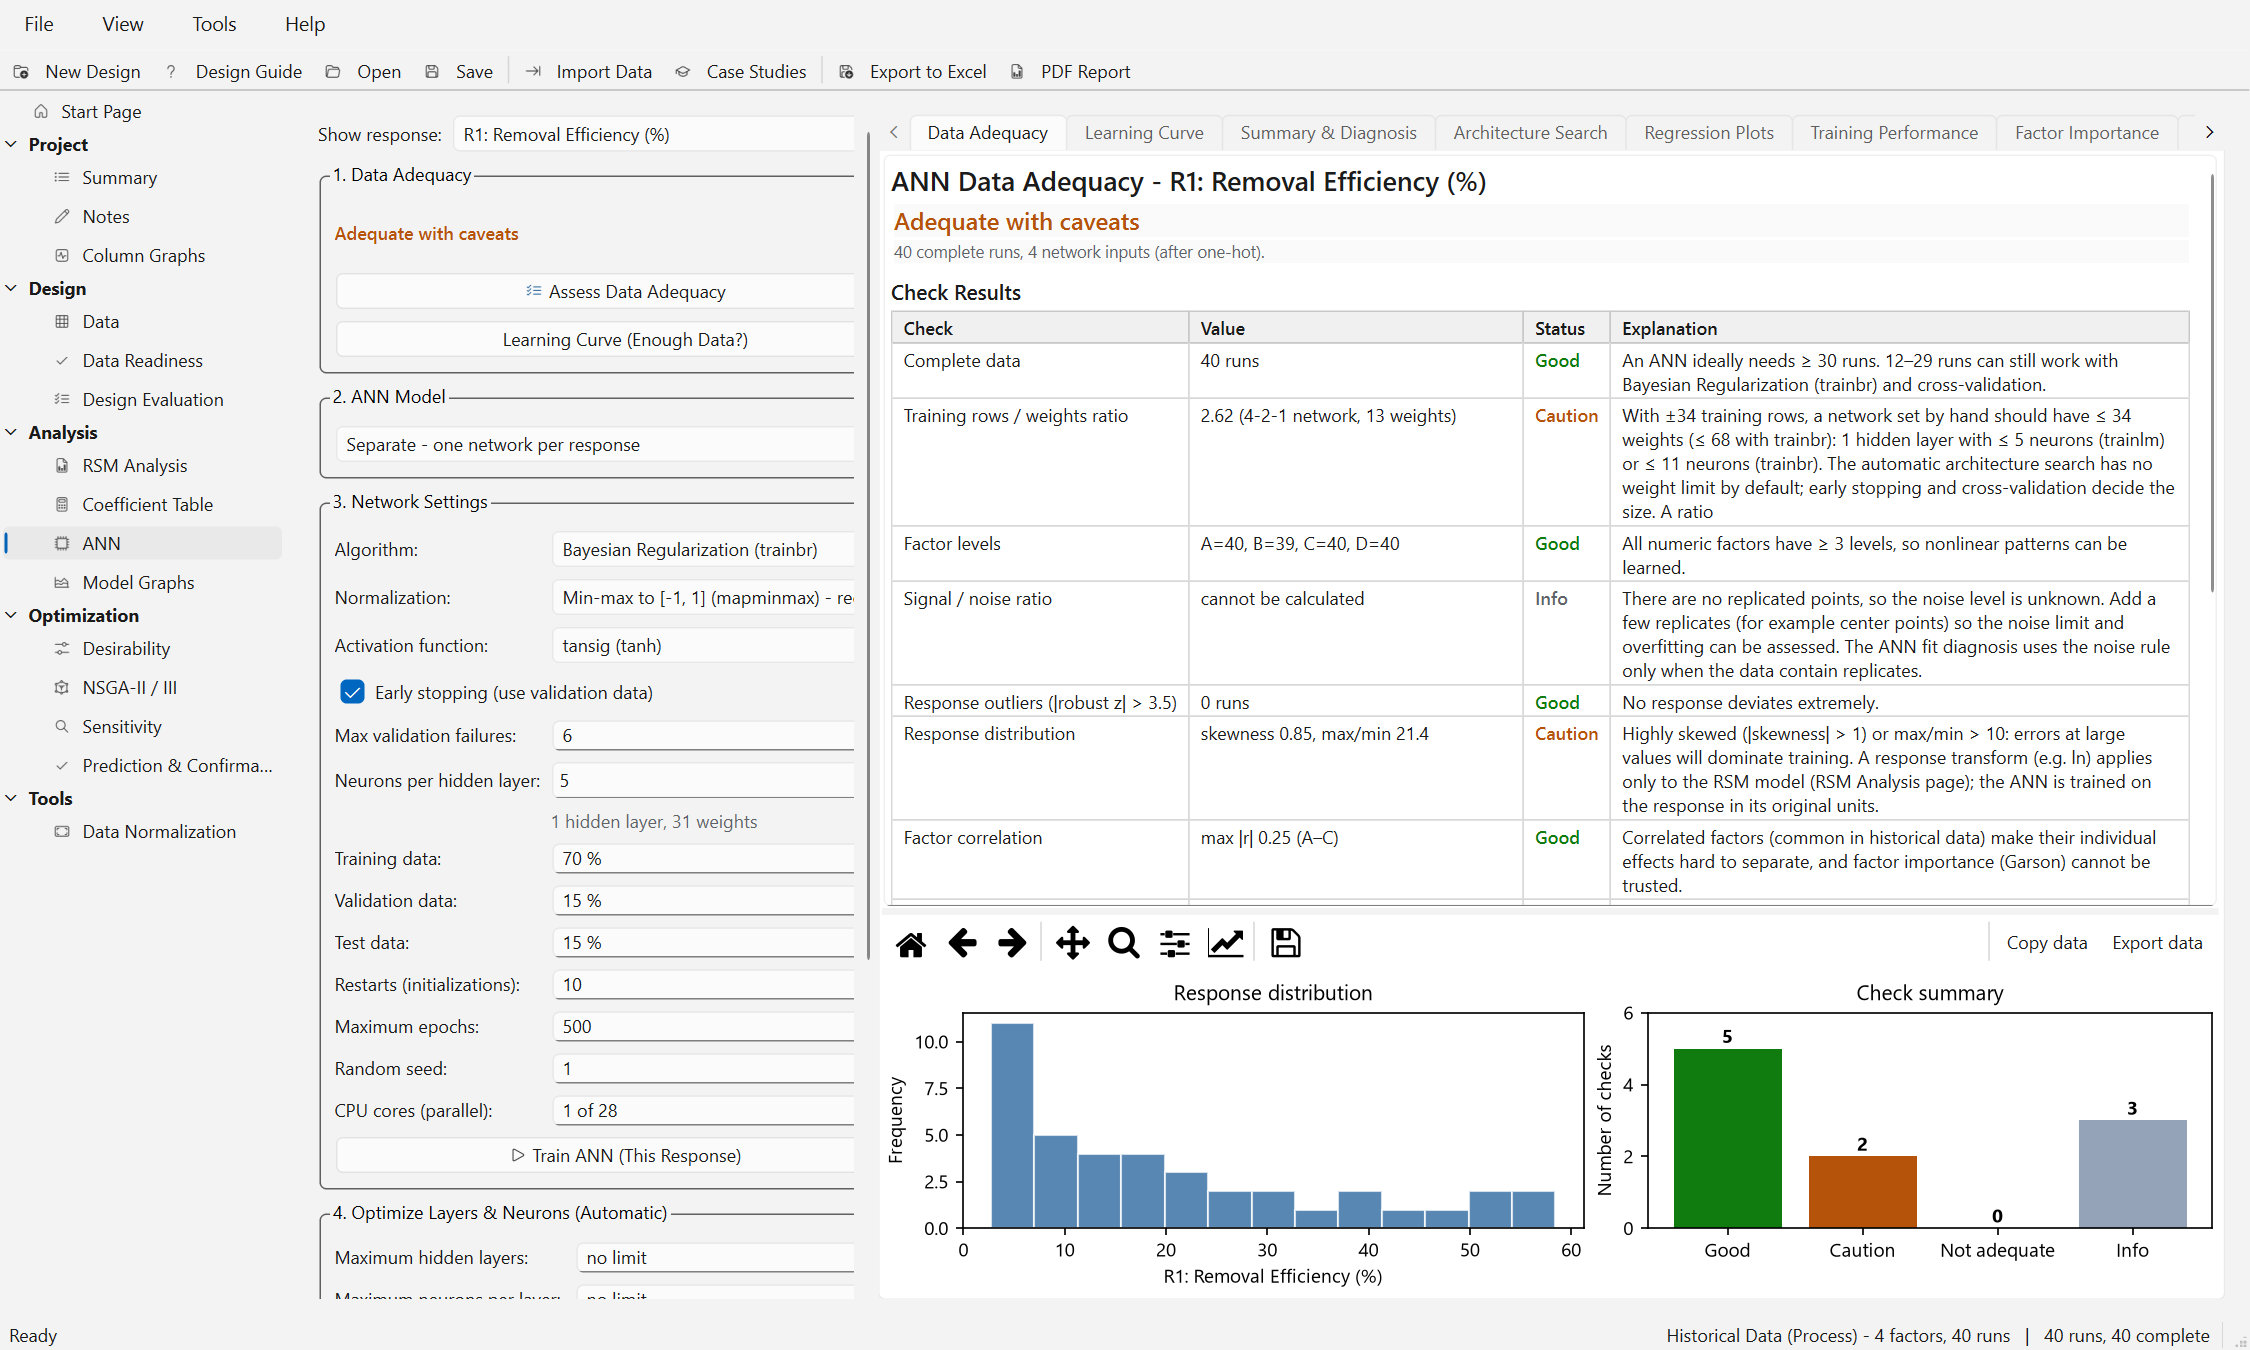
\includegraphics[width=\linewidth]{ann_adequacy.png}
\caption{\ui{Data Adequacy} tab for the dye adsorption case: verdict ``Adequate with caveats'', the table of
checks, the response histogram and the summary of statuses (5 Good, 2 Caution, 3 Info).}
\label{fig:ch07-adequacy}
\end{figure}

\paragraph{Skewed responses.} When the \ui{Response distribution} check gives Caution, its explanation reads
``Highly skewed (|skewness| > 1) or max/min > 10: errors at large values will dominate training. A response
transform (e.g. ln) applies only to the RSM model (RSM Analysis page); the ANN is trained on the response in its
original units.'' The recommendation adds: ``Skewed response: a response transform (e.g. ln) on the RSM Analysis
page applies to the RSM model only. The ANN is trained on the response in its original units; the Normalization
options only rescale it linearly and do not reduce the skewness.'' The normalization maps the response to
$[-1,1]$, but large values continue to dominate the squared error, so judge the network also by its relative
errors (AAD) and by the residuals at small response values.

\section{Check A: cross-validated architecture search}\label{sec:ch07-search}

\paragraph{Purpose.} The number of hidden layers and neurons controls the flexibility of the network: too few
neurons underfit, too many fit the noise. The architecture search finds the smallest network that predicts new
data as well as any larger one, using cross-validation \citep{hastie2009} rather than a single random split.

\subsection{How to use}

\begin{enumerate}
  \item Set the algorithm, normalization, activation, \ui{Max validation failures:} and \ui{Random seed:} in
    \ui{3. Network Settings}. These settings are used for every candidate network.
  \item In \ui{4. Optimize Layers \& Neurons (Automatic)}, keep the defaults (Table~\ref{tab:ch07-search}) unless
    the computation is too long.
  \item Click \ui{Search Architecture (This Response)} for the shown response, or \ui{Optimize All Responses (One
    Click)} to search and train a network for every continuous response in turn. Tick \ui{When finished, use ANN
    for graphs/optimization} if the networks should immediately replace the RSM models.
  \item Follow the progress line, for example ``R1 - 2 hidden layers: architecture 3-3 (candidate 8)''. \ui{Stop}
    ends the search; the results so far are kept and marked as incomplete.
  \item When the search ends, the selected architecture is trained on all data with the \ui{Network Settings}
    (Section~\ref{sec:ch07-final}) and the \ui{Architecture Search} tab opens.
\end{enumerate}

\begin{table}[htbp]
\centering
\caption{Options of group \ui{4. Optimize Layers \& Neurons (Automatic)}.}\label{tab:ch07-search}
\begin{tabularx}{\linewidth}{@{}p{4.0cm}p{2.6cm}p{1.6cm}X@{}}
\toprule
Option & Values & Default & Meaning \\
\midrule
\ui{Maximum hidden layers:} & 0--1000 (0 = \ui{no limit}) & no limit & Upper limit on the depth. \\
\ui{Maximum neurons per layer:} & 0--1\,000\,000 (0 = \ui{no limit}) & no limit & Upper limit on the neurons in
  any layer. \\
\ui{Cross-validation (k-fold):} & 3--10 & 5 & Number of folds $k$. \\
\ui{Early stopping patience:} & 1--6 & 2 & Neuron growth stops after this many candidates in a row without a 1~\%
  improvement of the test error. \\
\ui{Weight limit (x training data):} & 0--1000 (0 = \ui{no limit}) & no limit & Maximum weights as a multiple of
  the training runs per fold. \\
\ui{When finished, use ANN for graphs/optimization} & on/off & off & Select the new networks as the model of the
  searched responses. \\
\bottomrule
\end{tabularx}
\end{table}

Some settings of the search are fixed: every candidate is trained with 3 restarts per data split, at most 300
epochs, early stopping always on and the convergence test of trainbr active. They keep the search fast; the final
network is trained afterwards with the full \ui{Network Settings}.

\subsection{Evaluation scheme}

At least 8 complete runs are required. With $N < 400$ runs, the runs are divided at random into $k$ folds
(\ui{Cross-validation (k-fold):}, at most $N$). Each fold is the test set once; of the remaining runs,
$\max(1, \operatorname{round}(0.15\,n_\text{rest}))$ are drawn as validation runs for early stopping (none if fewer
than 6 remain) and the rest are training runs. With $N \ge 400$ runs, a single 70/15/15~\% hold-out split is
used, and data sets above 4000 runs are searched on a random sample of 4000 runs (the final network is trained on
all data). For the dye case, every fold has 27 training, 5 validation and 8 test runs.

For every candidate architecture and every split, the best of the 3 restarts is chosen by the training plus
validation score of Eq.~\eqref{eq:ch07-score}; the test fold takes no part in the choice. The candidate is then
summarized by the mean NMSE over the splits on training, validation and test runs, $E_\text{tr}$, $E_\text{va}$
and $E_\text{te}$ (Eq.~\eqref{eq:ch07-nmse}), by the standard error of $E_\text{te}$,
\begin{equation}
  \text{SE} = \frac{\operatorname{sd}(E_{\text{te},1},\dots,E_{\text{te},k})}{\sqrt{k}}
  \quad\text{(k-fold)}, \label{eq:ch07-se}
\end{equation}
(for the hold-out split, the standard deviation of the normalized squared errors of the test runs divided by
$\sqrt{n_\text{te}}$), by the training $R^2 = 1 - E_\text{tr}$, the test $R^2 = Q^2 = 1 - E_\text{te}$, the mean
best epoch, and the test RMSE $\sqrt{E_\text{te}\operatorname{var}(y)}$ in response units.

\subsection{Growth rule: early stopping on three levels}\label{sec:ch07-growth}

\begin{enumerate}
  \item \emph{Weights.} Each training run stops on its validation runs (Section~\ref{sec:ch07-split}).
  \item \emph{Neurons.} A layer is grown through the sequence 1, 2, 3, 4, 5, 6, 8, 10, 12, 15, 20, 25, 30, 40,
    50, 64, 80, 100, 128, 160, 200 neurons, continued by factors of 1.25 without end (cut at \ui{Maximum neurons
    per layer:} if set). With $B$ the best test error so far in this layer, a candidate counts as an improvement
    if
    \begin{equation}
      E_\text{te} < 0.99\,B, \label{eq:ch07-grow}
    \end{equation}
    that is, at least 1~\% lower; otherwise a failure is counted. Growth stops after \ui{Early stopping patience:}
    failures in a row, or when the next candidate would exceed the weight limit.
  \item \emph{Layers.} For depth $d = 2, 3, \dots$ the two best architectures of depth $d-1$ (lowest $E_\text{te}$)
    are used as prefixes, and a new last layer is grown on each of them as above. If the best test error at depth
    $d$ is not at least 1~\% below the best of all shallower networks, adding layers stops (``Layer early stopping:
    \dots''). The search also stops at \ui{Maximum hidden layers:}.
\end{enumerate}
The weight limit is
\begin{equation}
  W_\text{max} = \max\!\left(\rho\, n_\text{train},\; W(n_\text{in},[1],n_\text{out})\right), \label{eq:ch07-wlimit}
\end{equation}
with $\rho$ = \ui{Weight limit (x training data):} and $n_\text{train}$ the smallest training set over the
splits. The default is \emph{no limit}: the size is then limited only by the three levels of early stopping. A
limit such as $\rho = 2$ reproduces the classical rule of thumb for trainbr and shortens searches on large
networks, but it can exclude the best architecture when the data are rich.

\subsection{Overfit and underfit classification of candidates}

After the search, each candidate is classified relative to the best test error of all candidates,
$E^* = \min E_\text{te}$:
\begin{itemize}
  \item \ui{Overfitting} if the data contain replicated runs, $E_\text{tr} < 0.5\,\nu$ and $E_\text{te} > 1.05
    E^*$ (noise rule, Eq.~\eqref{eq:ch07-noise});
  \item \ui{Overfitting} if $E_\text{te} > 2E_\text{tr}$ and $E_\text{te} > 1.2E^*$ and $E_\text{te} -
    E_\text{tr} > 0.02$;
  \item \ui{Underfitting} if $E_\text{tr} > 1.5E^*$ and $E_\text{te} < 1.5E_\text{tr} + 0.02$ and $E_\text{te} >
    1.2E^*$ and $E_\text{te} - E^* > 0.01$;
  \item \ui{Good fit} otherwise.
\end{itemize}
These rules differ from the single-split rules of Section~\ref{sec:ch07-diagnose} because they are relative: a
candidate is called overfitting only if its test error is also clearly worse (more than 20~\%) than the best
candidate. A network whose test error is close to the best is not penalized for a low training error.

\subsection{Selection: the one-standard-error rule}

The selected network is the simplest one whose cross-validated error cannot be distinguished from the best
\citep{hastie2009}:
\begin{enumerate}
  \item The pool contains all candidates with status \ui{Good fit} (all candidates if none is good).
  \item The best raw candidate is the pool member with the lowest $E_\text{te}$.
  \item The threshold is
    \begin{equation}
      \tau = E_\text{te}(\text{best raw}) + \max\!\left(\text{SE}(\text{best raw}),\, 0.002\right).
      \label{eq:ch07-1se}
    \end{equation}
  \item Among the pool members with $E_\text{te} \le \tau$, the one with the fewest weights is selected (ties:
    fewer layers, then lower $E_\text{te}$).
\end{enumerate}
The floor 0.002 treats test $R^2$ differences below 0.002 as equal. Choosing the smaller network within one
standard error lowers the risk of overfitting at no measurable cost in accuracy.

\subsection{Final training after the search}\label{sec:ch07-final}

The selected architecture is trained on all runs with the \ui{Network Settings} (default 10 restarts, 500
epochs, the random 70/15/15~\% split of the seed). Early stopping is switched on whenever the validation
percentage is above zero. The cross-validated status and $R^2$ values of the selected candidate are attached to
the model and become its main diagnosis.

At the same time the \emph{current RSM model} of the response (the terms selected on the \ui{RSM Analysis} page)
is refitted on the training and validation runs of every split and scored on the same test runs. This gives an
RSM test $R^2$ that can be compared fairly with the ANN. For small response surface designs it is often very low
or negative: when a few runs of a Box-Behnken or central composite design are left out, the remaining runs no
longer support the quadratic model well. The report then adds a note and recommends to compare also with the RSM
Predicted $R^2$ (which is a leave-one-out statistic).

\subsection{Output and how to read it}

The \ui{Architecture Search} tab (Figure~\ref{fig:ch07-search}) contains:
\begin{itemize}
  \item a scatter plot of training $R^2$ (hollow) and test $R^2$ (filled) against the number of weights, colored
    by status; the selected network is circled and the RSM test $R^2$ is a dotted line. A large vertical gap
    between the two markers indicates overfitting; both low indicates underfitting;
  \item a bar chart of the best network per number of hidden layers;
  \item the settings of the search, the table of the best network per depth with an ``RSM (current model)'' row,
    the selected network, the number of candidates excluded as overfitting or underfitting, the stopping notes and
    the conclusion ``ANN predicts new data better than RSM'' or ``RSM predicts new data as well as or better than
    ANN'' (assessed on the same test data);
  \item the table \ui{All Architectures (Sorted by Test Error)} with training, validation and test $R^2$, SE, mean
    best epoch and status; the selected row is bold. If the 1-SE rule chose a smaller network than the best raw
    one, a note says so.
\end{itemize}
The status line lists the result per response, for example ``Done. R1: 1 layer (3) - Good fit''.

\begin{figure}[htbp]
\centering
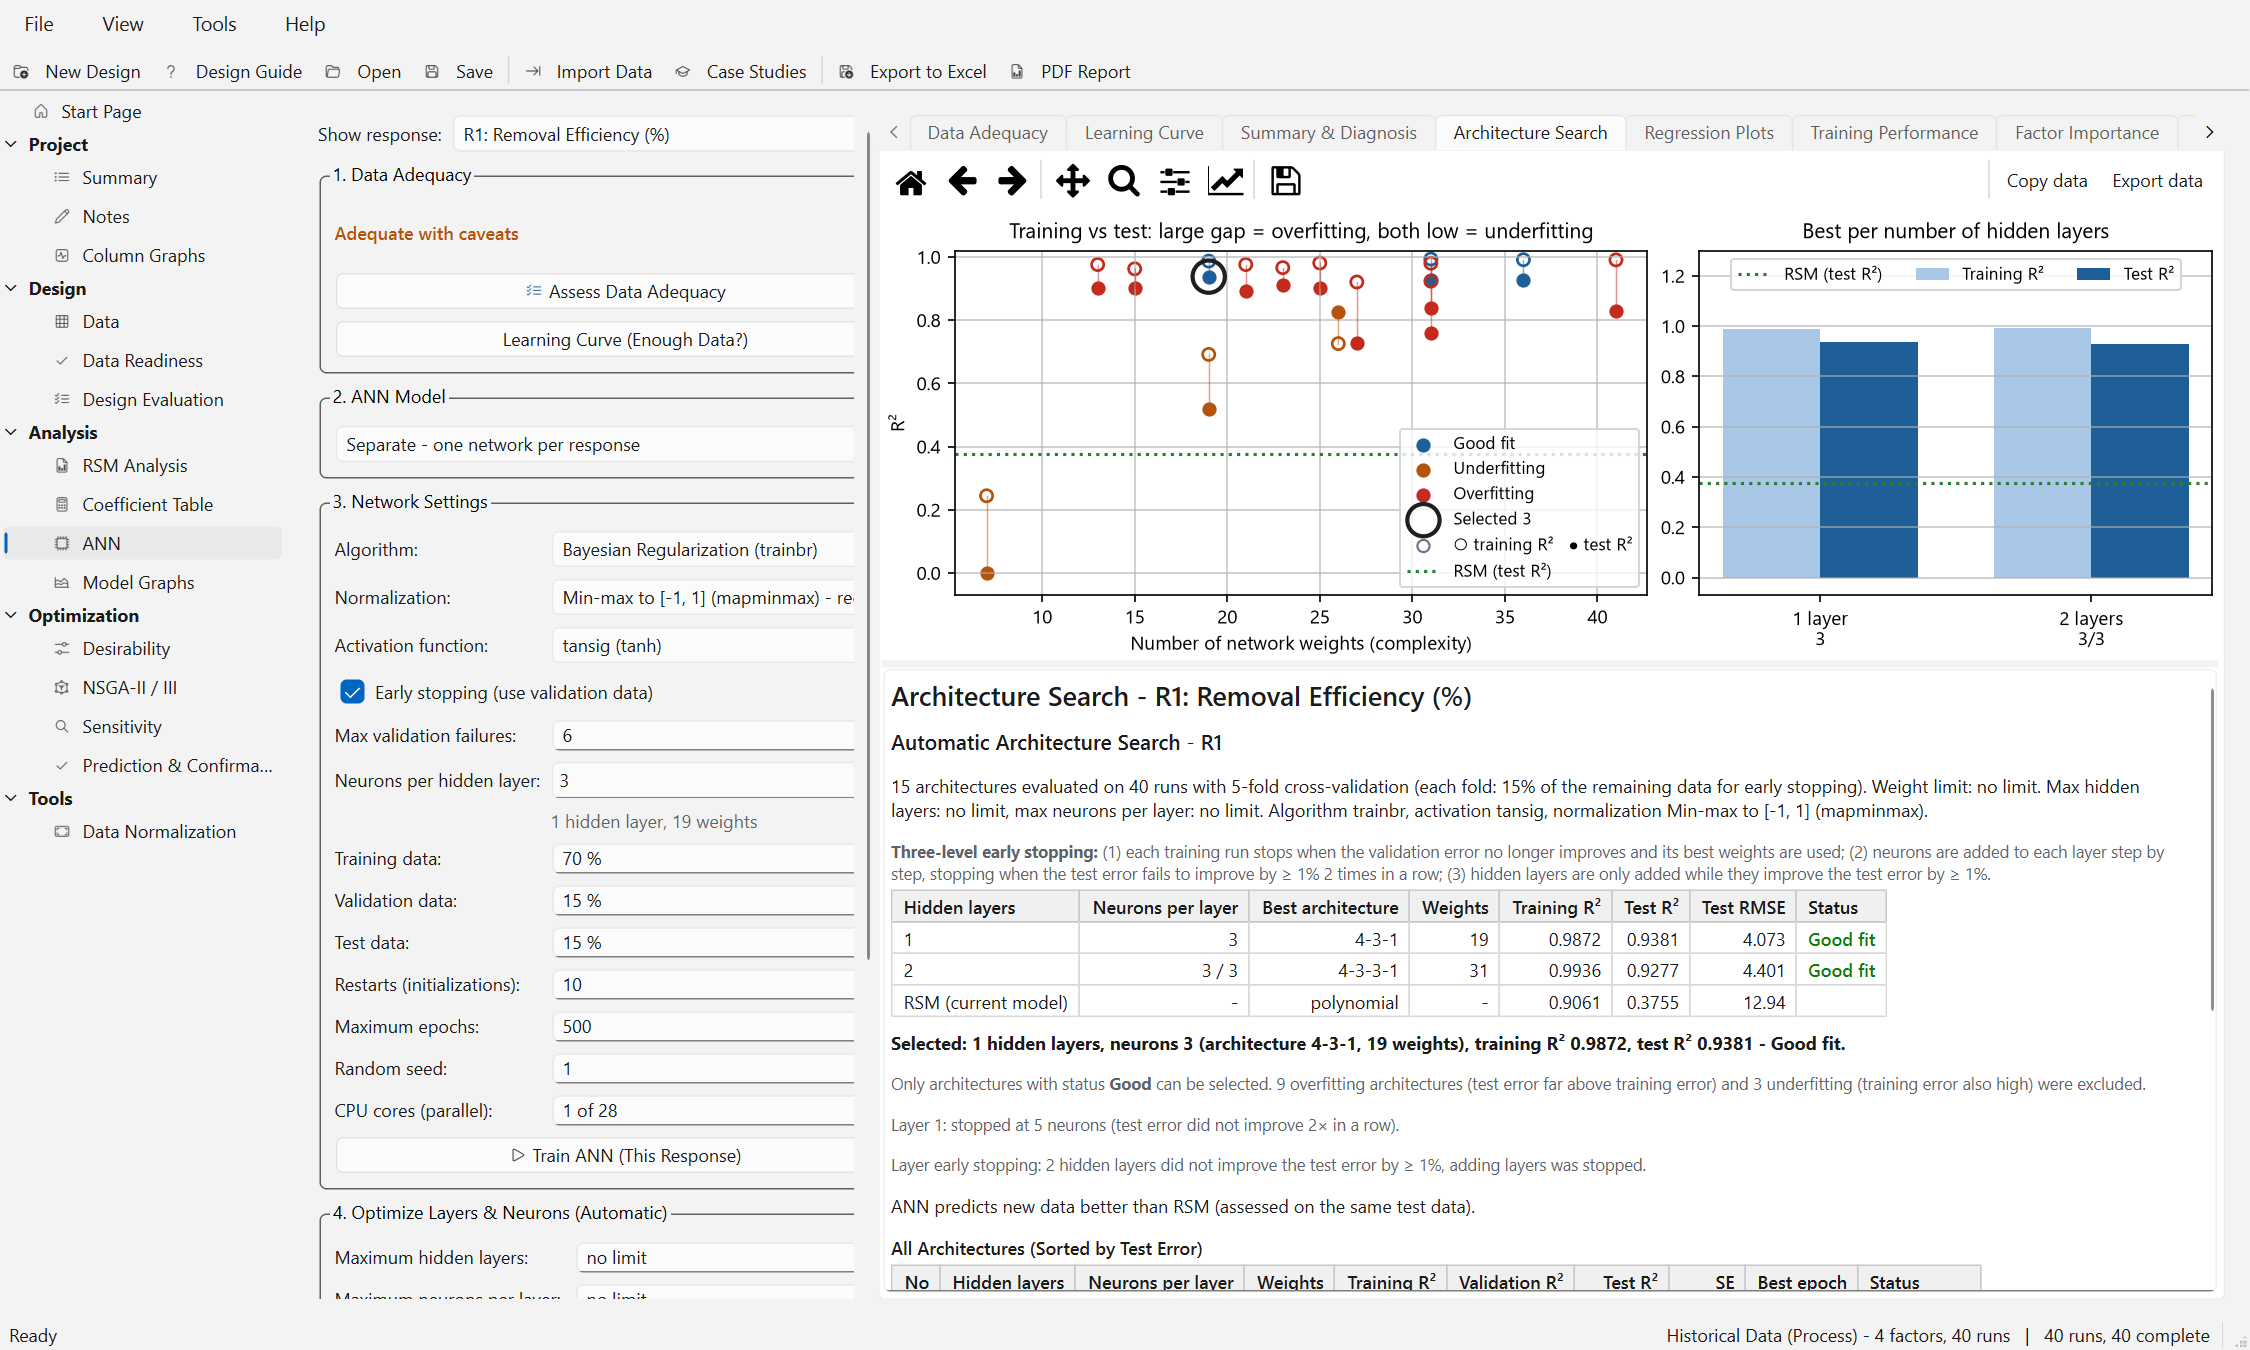
\includegraphics[width=\linewidth]{ann_search.png}
\caption{\ui{Architecture Search} tab for the dye adsorption case with the default settings: 15 candidate networks,
the selected 4-3-1 network (circled), the best network per depth and the RSM test $R^2$ of 0.3755 (dotted).}
\label{fig:ch07-search}
\end{figure}

\subsection{Example: dye adsorption}

With the default settings the search evaluates 15 architectures with 5-fold cross-validation in about 5~s on one
core. Table~\ref{tab:ch07-searchex} lists them in the order of evaluation.

\begin{table}[htbp]
\centering
\caption{All candidates of the architecture search for the dye case (5-fold cross-validation, NMSE averaged over the
folds). $^*$ = selected.}\label{tab:ch07-searchex}
\begin{tabular}{@{}lrrrrrrl@{}}
\toprule
Neurons & $W$ & $E_\text{tr}$ & $E_\text{te}$ & SE & Train $R^2$ & Test $R^2$ & Status \\
\midrule
1       &  7 & 0.7553 & 0.9990 & 0.2275 & 0.245 & 0.001 & Underfitting \\
2       & 13 & 0.0236 & 0.0974 & 0.0171 & 0.976 & 0.903 & Overfitting \\
3$^*$   & 19 & 0.0128 & 0.0619 & 0.0097 & 0.987 & 0.938 & Good fit \\
4       & 25 & 0.0187 & 0.0978 & 0.0263 & 0.981 & 0.902 & Overfitting \\
5       & 31 & 0.0194 & 0.1622 & 0.0652 & 0.981 & 0.838 & Overfitting \\
3/1     & 21 & 0.0237 & 0.1074 & 0.0473 & 0.976 & 0.893 & Overfitting \\
3/2     & 26 & 0.2738 & 0.1735 & 0.0587 & 0.726 & 0.827 & Underfitting \\
3/3     & 31 & 0.0064 & 0.0723 & 0.0158 & 0.994 & 0.928 & Good fit \\
3/4     & 36 & 0.0084 & 0.0726 & 0.0178 & 0.992 & 0.927 & Good fit \\
3/5     & 41 & 0.0089 & 0.1718 & 0.1276 & 0.991 & 0.828 & Overfitting \\
2/1     & 15 & 0.0372 & 0.0973 & 0.0178 & 0.963 & 0.903 & Overfitting \\
2/2     & 19 & 0.3080 & 0.4810 & 0.2682 & 0.692 & 0.519 & Underfitting \\
2/3     & 23 & 0.0335 & 0.0870 & 0.0114 & 0.967 & 0.913 & Overfitting \\
2/4     & 27 & 0.0789 & 0.2732 & 0.1003 & 0.921 & 0.727 & Overfitting \\
2/5     & 31 & 0.0762 & 0.2404 & 0.1518 & 0.924 & 0.760 & Overfitting \\
\bottomrule
\end{tabular}
\end{table}

The course of the search can be followed with the rules above:
\begin{itemize}
  \item Layer 1: 1, 2 and 3 neurons each improve the test error; 4 neurons (0.0978) and 5 neurons (0.1622) fail
    twice in a row, so growth stops at 5 neurons (``Layer 1: stopped at 5 neurons (test error did not improve 2×
    in a row).'').
  \item Layer 2 is grown on the two best one-layer networks, 3 and 2 neurons. The best two-layer network, 3/3,
    has $E_\text{te} = 0.0723$, which is not 1~\% below 0.0619, so no third layer is tried (``Layer early stopping:
    2 hidden layers did not improve the test error by $\ge$ 1\%, adding layers was stopped.'').
  \item With $E^* = 0.0619$, the network with 2 neurons is classified as overfitting: its test error 0.0974 is
    more than twice its training error 0.0236 and more than $1.2E^* = 0.0743$. One neuron is underfitting
    ($E_\text{tr} = 0.755$). Nine candidates are overfitting, three underfitting and three good.
  \item 1-SE rule: $\tau = 0.0619 + \max(0.0097, 0.002) = 0.0716$. The good networks 3/3 (0.0723) and 3/4 (0.0726)
    are just above $\tau$, so the selected network is the best raw one, 4-3-1 with 19 weights (training $R^2$
    0.9872, test $R^2$ 0.9381).
  \item RSM on the same folds: training $R^2$ 0.9061, test $R^2$ 0.3755 (test RMSE 12.94 against 4.073 for the
    ANN), so ``ANN predicts new data better than RSM''. The four-factor quadratic model cannot follow the pH
    optimum and the saturation of this response.
\end{itemize}

\section{Fit diagnosis after a search}\label{sec:ch07-diagnosis}

The \ui{Summary \& Diagnosis} tab (Figure~\ref{fig:ch07-summary}) starts with the architecture, the algorithm, the
number of weights, the normalization, the data split, the number of epochs with the stop reason, the effective
parameters $\gamma$ (trainbr) and the number of restarts. The \ui{Fit Diagnosis} follows.
\begin{itemize}
  \item \emph{After an architecture search}, the headline is the cross-validated status of the selected
    candidate, for example ``Good fit (result of 5-fold cross-validation during architecture search)'', with the
    training, validation and test $R^2$ averaged over the folds. The section \ui{Single Train/Test Split (Final
    Model)} then gives the status of the final network on its one random split as secondary information, with the
    reason (``Single split: \dots''). The suggestions (reduce or add neurons, run the search) follow the
    cross-validated status.
  \item \emph{After training by hand}, the only status is that of the single split, marked ``(single train/test
    split)''.
  \item If the validation and test sets together have fewer than 10 runs, a note warns that the single-split
    diagnosis is uncertain.
  \item A table gives $R^2$ and NMSE of the single split for training, validation and test data (and the
    measurement noise limit $1-\nu$ when replicates exist), followed by the epoch whose weights were used, the
    stop reason and the criteria of both diagnoses.
\end{itemize}
Further down are the run numbers of each set (\ui{Data Split (Random, Automatic)}), the \ui{Performance} table
(Eq.~\eqref{eq:ch07-metrics}), an \ui{RSM vs ANN Comparison} on all data and on the ANN test runs, the relative
factor importance, and a red warning if the network has more weights than training targets.

Note that in the \ui{RSM vs ANN Comparison} on this tab, RSM was fitted on all runs, including the ANN test runs,
which favors RSM. The fair comparison is the one on the \ui{Architecture Search} tab or the RSM Predicted $R^2$,
as the note under the table says.

\paragraph{Example.} For the final 4-3-1 network of the dye case (Figure~\ref{fig:ch07-summary}), the split is 28
training, 6 validation and 6 test runs. Training stopped at epoch 20 by early stopping; the weights of epoch 7
were used. The headline is ``Good fit'' from 5-fold cross-validation (training $R^2$ 0.9872, validation 0.9313,
test 0.9381). On the single split the status is ``Overfitting'': training NMSE 0.0215, validation 0.0105, test
0.1466, and $(0.0105+0.1466)/2 = 0.079$ is 3.6 times the training error. Six test runs are too few to decide this:
one or two poorly predicted runs triple the test error. The cross-validated result, which uses every run once as a
test run, is the reliable one. Because epoch 7 lies inside the warm-up of 15 epochs, the first line reads
``effective parameters $\gamma$ not estimated yet (best epoch 7 lies within the warm-up; $\gamma$ is first
estimated after epoch 15)''.

\begin{figure}[htbp]
\centering
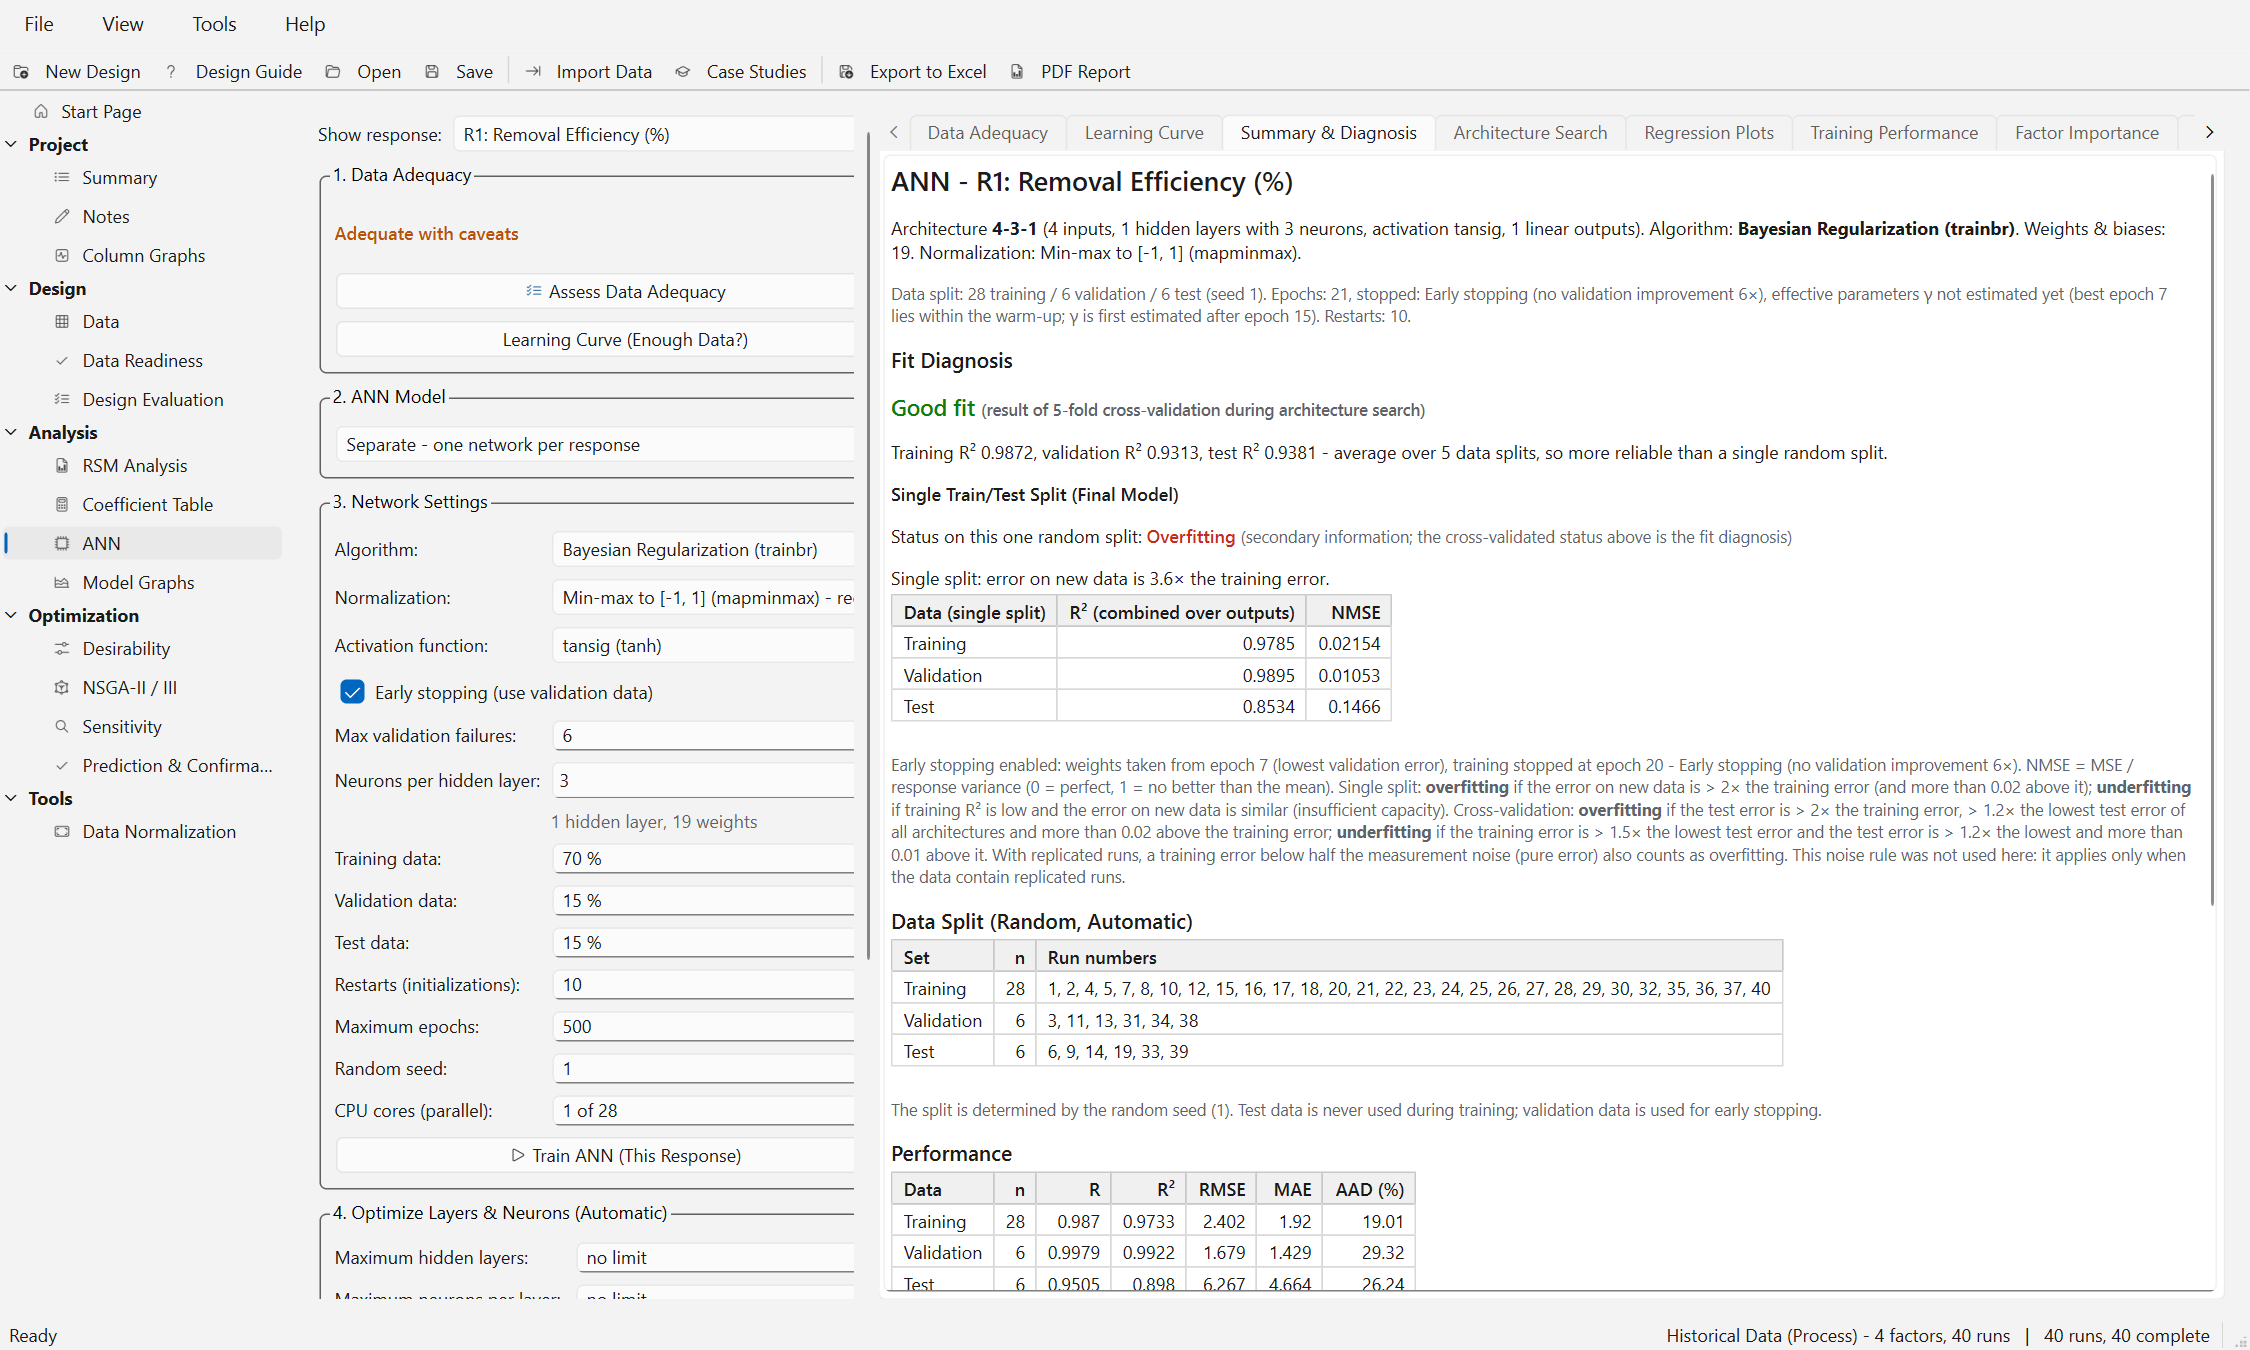
\includegraphics[width=\linewidth]{ann_summary.png}
\caption{\ui{Summary \& Diagnosis} tab of the selected 4-3-1 network: cross-validated ``Good fit'' as the headline,
the single split shown separately as ``Overfitting'', and the data split and performance tables.}
\label{fig:ch07-summary}
\end{figure}

\paragraph{When the diagnosis is poor.} \emph{Underfitting} (both errors high): allow more neurons or layers
(remove limits), increase \ui{Maximum epochs:} or \ui{Restarts (initializations):}, or check that the response is
not dominated by noise. \emph{Overfitting} (cross-validated): use trainbr with early stopping, set a weight limit,
or add runs; if every network overfits, the data are too few for an ANN and RSM is the better choice.
\emph{Cross-validated good fit but single split overfitting}: accept the cross-validated result, but expect
predictions with an error near the test RMSE of the search (4.07 in the example), not the training RMSE.

\section{Check B: learning curve}\label{sec:ch07-learning}

\paragraph{Purpose.} The learning curve answers ``Would more runs still improve the network, and roughly how
many?''. The network is trained on growing subsets of the data and tested on runs that are never used for
training. If the test $R^2$ still rises at the full data size, more runs would help; if it has flattened, the
remaining error comes from noise or from the model, not from the amount of data.

\subsection{How to use}

\begin{enumerate}
  \item Select the response and click \ui{Learning Curve (Enough Data?)}. The response must be continuous and have
    at least 12 complete runs.
  \item The network size is that of the response's trained network (its layers, activation, algorithm and
    normalization); without one, the entry \ui{Neurons per hidden layer:} and the current settings are used. A
    network that was switched to Adam automatically is trained with trainbr. The seed is \ui{Random seed:}.
  \item The \ui{Learning Curve} tab opens and the status line reads, for example, ``Learning curve finished: more
    data would still help (run estimate unreliable)''.
\end{enumerate}
Every point of the curve uses fixed settings that do not depend on \ui{Network Settings}: 2 restarts, at most 300
epochs, early stopping after 6 validation failures, and the trainbr convergence test.

\subsection{Procedure as implemented}

\begin{enumerate}
  \item The number of repeats is $R = 10$ for $N < 60$, 6 for $N < 400$ and 4 otherwise.
  \item In each repeat, $n_\text{te} = \max(3, \operatorname{round}(0.2N))$ runs are drawn as a fixed test set; the
    other runs form the pool.
  \item For the fractions $f = 0.3, 0.4, \dots, 1.0$ of the pool, the first $n = \max(5, \operatorname{round}(f\,
    n_\text{pool}))$ runs of the shuffled pool are used for fitting (nested subsets). Of these, $\max(1,
    \operatorname{round}(0.15\,n))$ are validation runs when $n \ge 10$. The network is trained on the subset and
    its NMSE on the fixed test set is recorded (with the variance of all runs in the denominator).
  \item The current RSM model is fitted on the same subsets and tested on the same runs; subsets too small for its
    terms give no value.
  \item For each size the median and the quartiles over the repeats are shown.
\end{enumerate}

\subsection{Power-law fit and runs needed}

The median test NMSE is fitted with the power law
\begin{equation}
  e(n) = a + b\,n^{-c}, \qquad a, b \ge 0, \label{eq:ch07-powerlaw}
\end{equation}
which is a common model of learning curves \citep{figueroa2012}. Here $a$ is the error that would remain with
unlimited data, so $R^2_\infty = 1 - a$ is the upper limit of the test $R^2$. The exponent is searched on the grid
$c = 0.20, 0.25, \dots, 2.50$ (47 values); for each $c$, $a$ and $b$ are found by least squares (with $a = 0$ and
$b$ refitted if $a$ would be negative), and the $c$ with the smallest residual sum of squares is kept. When there
are at least six sizes, the two smallest are left out of the fit because they are too noisy.

The number of fitting runs at which the test $R^2$ comes within $0.01$ of its limit is
\begin{equation}
  b\,n^{*\,-c} = 0.01 \quad\Longrightarrow\quad n^* = \left\lceil \left(\frac{b}{0.01}\right)^{1/c}\right\rceil.
  \label{eq:ch07-nstar}
\end{equation}
To express its uncertainty, the repeats are resampled 200 times (bootstrap), the median curve is refitted and
$n^*$ recomputed each time. The reported value $n^*_\text{med}$ is the median of the bootstrap values, with their
quartiles as the range. Since $n^*$ counts runs used for fitting, the total number of runs including the test
share is
\begin{equation}
  N_\text{total} = \left\lceil \frac{n^*_\text{med}}{1 - n_\text{te}/N} \right\rceil. \label{eq:ch07-ntotal}
\end{equation}

\subsection{Statuses and messages}

With $n_\text{full}$ the largest subset of the curve:
\begin{itemize}
  \item $n^*_\text{med} \le n_\text{full}$: ``\textbf{The data is sufficient.} The curve has flattened \dots''.
  \item $n_\text{full} < n^*_\text{med} \le 5\,n_\text{full}$: ``\textbf{More data would still help.} \dots{}
    Estimate: about $N_\text{total}$ runs in total (range \dots; add about \dots{} runs) \dots''. This is an
    extrapolation: add runs in stages (for example half first) and repeat the learning curve.
  \item $n^*_\text{med} > 5\,n_\text{full}$: ``\textbf{The data is still far from sufficient.}'' The message states
    the test used (more than 5 times the largest training set, that is more than $5N$ runs in total) and suggests
    RSM, fewer factors or narrower ranges.
  \item $N < 25$ overrides the status: ``\textbf{Too little data (\dots{} runs) for a reliable learning curve.}''
    The subsets are then too small to show a trend.
\end{itemize}
A reliability warning is added (``The run estimate is unreliable: \dots'') when the fitted exponent lies at the
edge of the grid ($c = 0.2$ or $2.5$), when the fitted error limit is $a = 0$ (the curve predicts a perfect fit with
unlimited data), or when the interquartile range of the bootstrap estimate is very wide (upper/lower quartile $>
3$). The estimate is not changed; it should then be read only as an indication of \emph{whether} more runs help,
not \emph{how many}.

The report ends with the ANN and RSM test $R^2$ at the full size (``RSM usually wins with little data; ANN needs
more data to catch up'' when RSM is better) and a table per size: training data, ANN test $R^2$ (median and
quartiles), ANN training $R^2$ and RSM test $R^2$. The plot shows the median test $R^2$ with an interquartile band,
the training $R^2$ (dashed), the RSM test $R^2$ (squares), and, for the statuses ``more'' and ``enough'', the
fitted curve and the estimated upper limit; for ``more'' a vertical line marks $n^*$.

\subsection{Example: dye adsorption}

Figure~\ref{fig:ch07-learning} shows the learning curve computed with the default entry of 5 neurons (before the
search). With $N = 40$ there are 10 repeats, 8 fixed test runs and fitting subsets of 10, 13, 16, 19, 22, 26, 29
and 32 runs. The median test $R^2$ rises from $-0.014$ at 10 runs to 0.898 at 26 runs and 0.876 at 32 runs; RSM
reaches only 0.429 at 32 runs and is strongly negative below 19 runs, where the 15 coefficients of the four-factor
quadratic model are barely or not estimable. The power-law fit (on the six largest sizes) gives $a = 0$, $b =
509.3$ and $c = 2.5$, so $R^2_\infty = 1.000$ and, from Eq.~\eqref{eq:ch07-nstar}, $(509.3/0.01)^{1/2.5} = 76.3$,
that is 77 runs; the bootstrap median is $n^*_\text{med} = 80$ (quartiles 76 and 88). With $n_\text{te}/N = 0.2$,
$N_\text{total} = 80/0.8 = 100$ runs (range 95 to 111), so about 60 runs should be added. Because $c$ lies at the
upper edge of the grid and $a = 0$, the report flags the estimate as unreliable. The sound conclusion is
qualitative: the ANN is still improving at 40 runs and more runs would help, but the number 100 should not be
taken literally. The plateau between 26 and 32 runs shows how noisy the curve is at this size.

\begin{figure}[htbp]
\centering
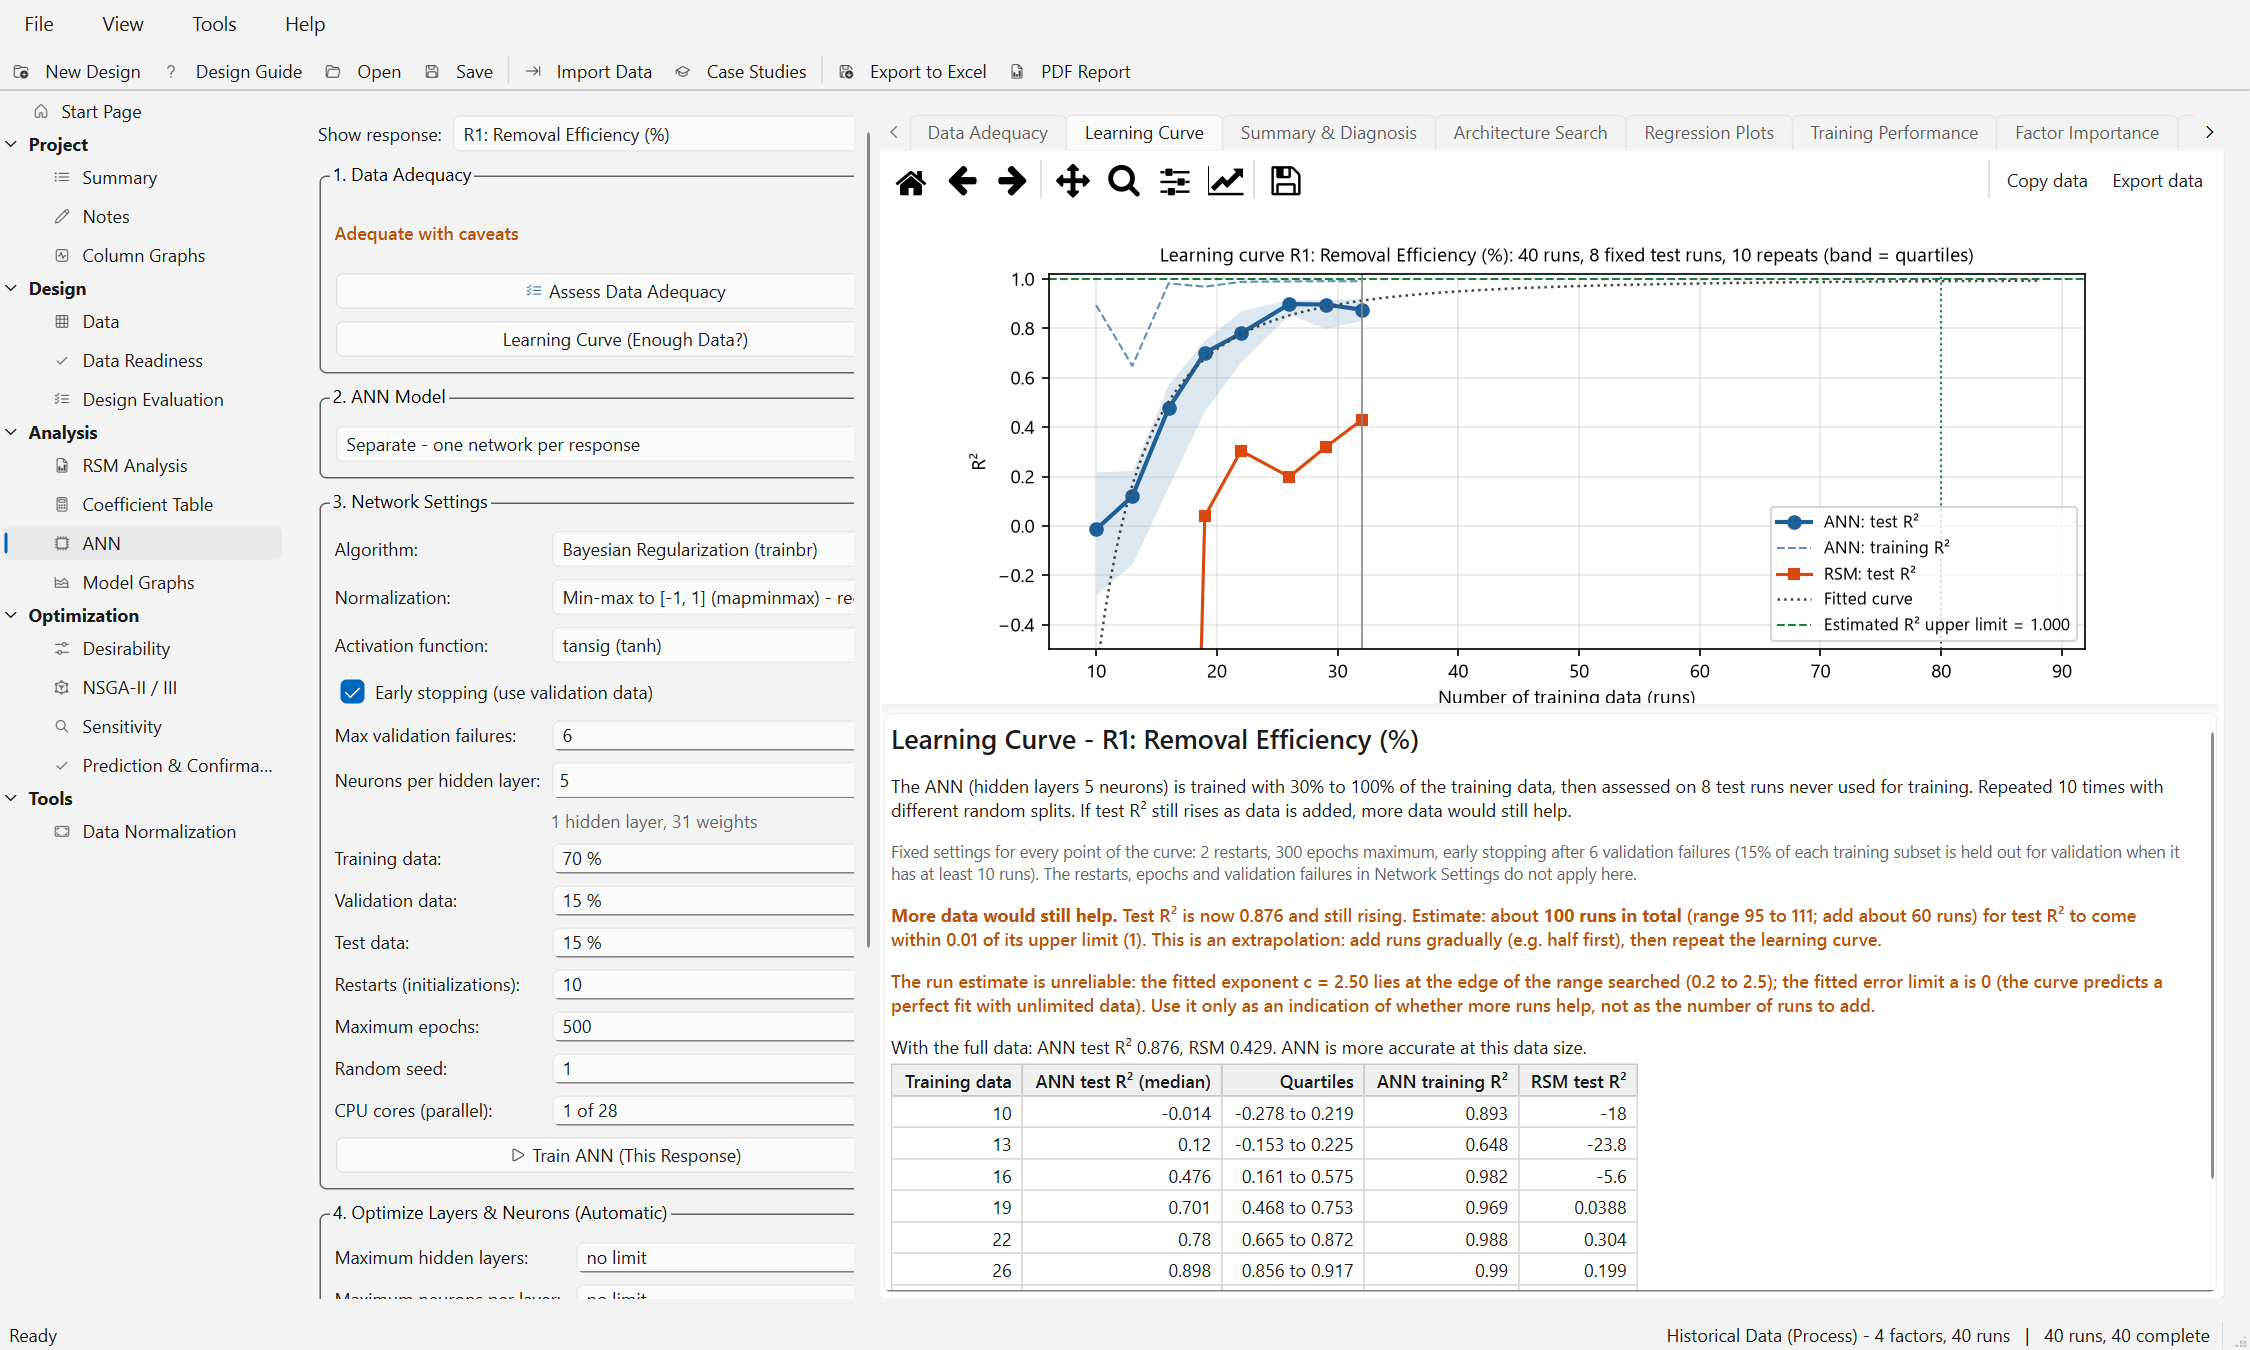
\includegraphics[width=\linewidth]{ann_learning_curve.png}
\caption{\ui{Learning Curve} tab for the dye case (1 hidden layer of 5 neurons): ANN test $R^2$ with interquartile
band, training $R^2$, RSM test $R^2$, fitted power law with the estimated upper limit and the line at $n^* = 80$
training runs; below, the message ``More data would still help'' with the reliability warning.}
\label{fig:ch07-learning}
\end{figure}

\paragraph{Limitations.} The curve depends on the network size used; run it with the network selected by the
search when available. Extrapolating a power law fitted on a handful of noisy points is uncertain, which is why the
bootstrap range and the warnings are shown. New runs should cover the factor space (the \ui{Data Readiness} page
suggests space-filling runs); runs repeated at existing points add little information for an ANN.

\section{Other result tabs}\label{sec:ch07-tabs}

\paragraph{Regression Plots.} Four panels (Training, Validation, Test, All) plot the network output against the
target with the 1:1 line (dotted) and a least-squares line; the title of each panel gives the correlation $R$
(Figure~\ref{fig:ch07-regression}). Points of the test panel far from the line are the runs the network predicts
poorly. For the dye network $R$ is 0.9870 (training), 0.9979 (validation), 0.9505 (test) and 0.9809 (all data).

\begin{figure}[htbp]
\centering
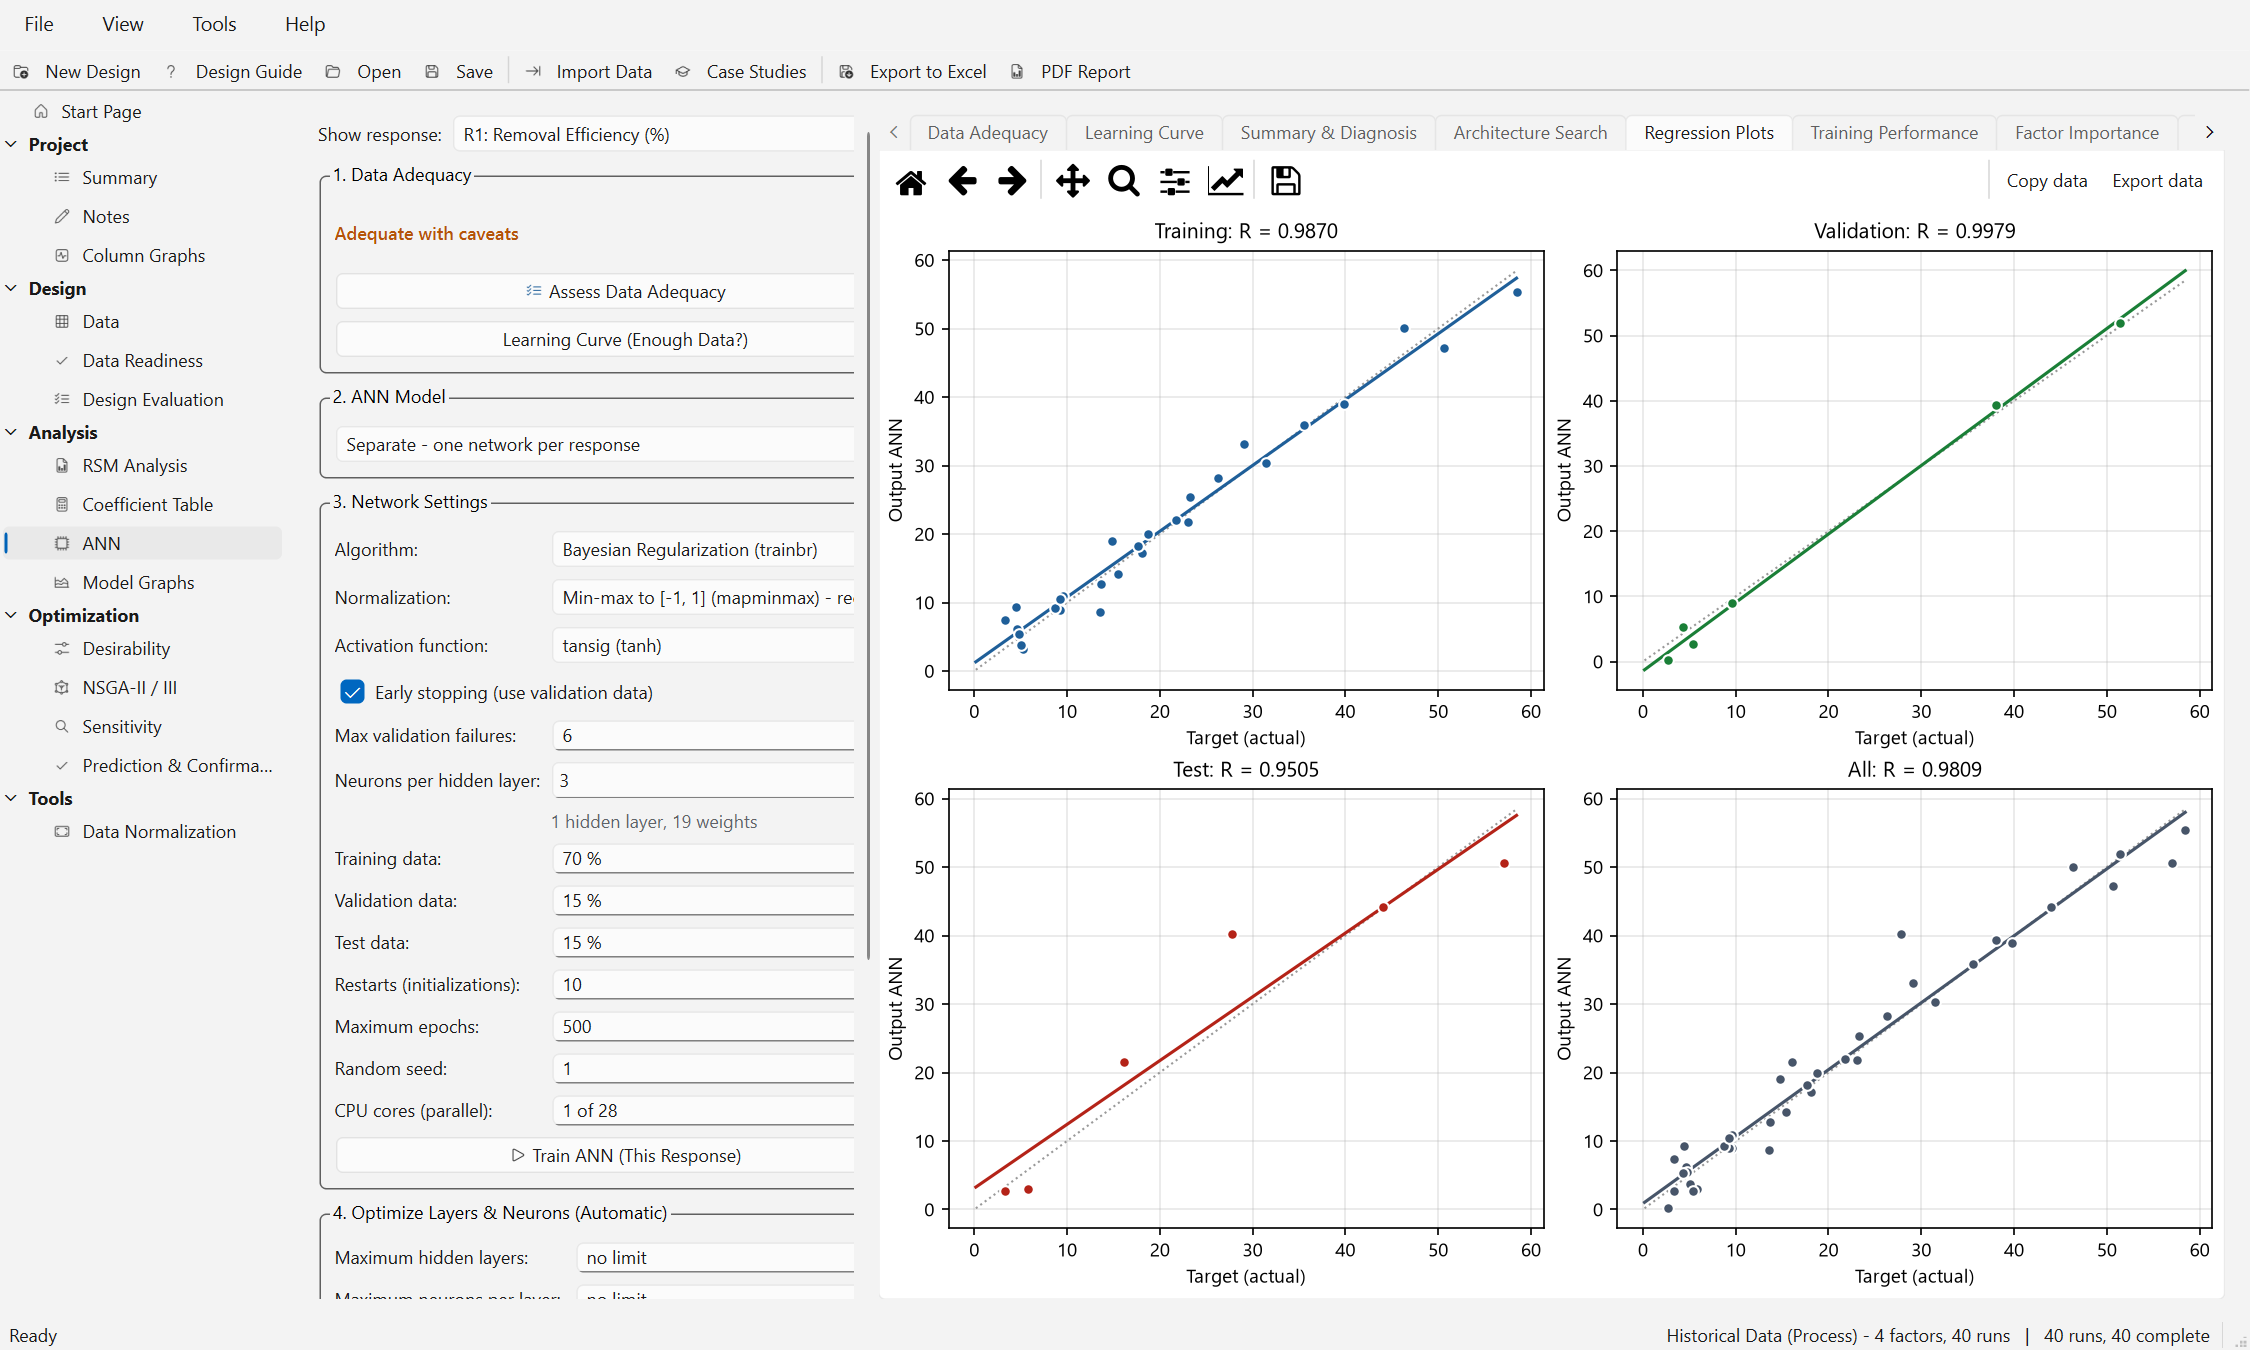
\includegraphics[width=\linewidth]{ann_regression.png}
\caption{\ui{Regression Plots} of the 4-3-1 network for training, validation, test and all data.}
\label{fig:ch07-regression}
\end{figure}

\paragraph{Training Performance.} The mean squared error on the normalized scale per epoch for training,
validation and test data, on a logarithmic axis (Figure~\ref{fig:ch07-performance}). A dotted vertical line marks
the epoch whose weights are used (``Weights used (epoch 7) - early stopping'') and a shaded band marks the epochs in
which the validation error did not improve. In the dye example the validation error reaches its minimum at epoch
7; with trainbr, failures are counted only from epoch 15, so training stops at epoch 20. A test curve that keeps
rising after the marked epoch is the typical picture that early stopping prevents.

\begin{figure}[htbp]
\centering
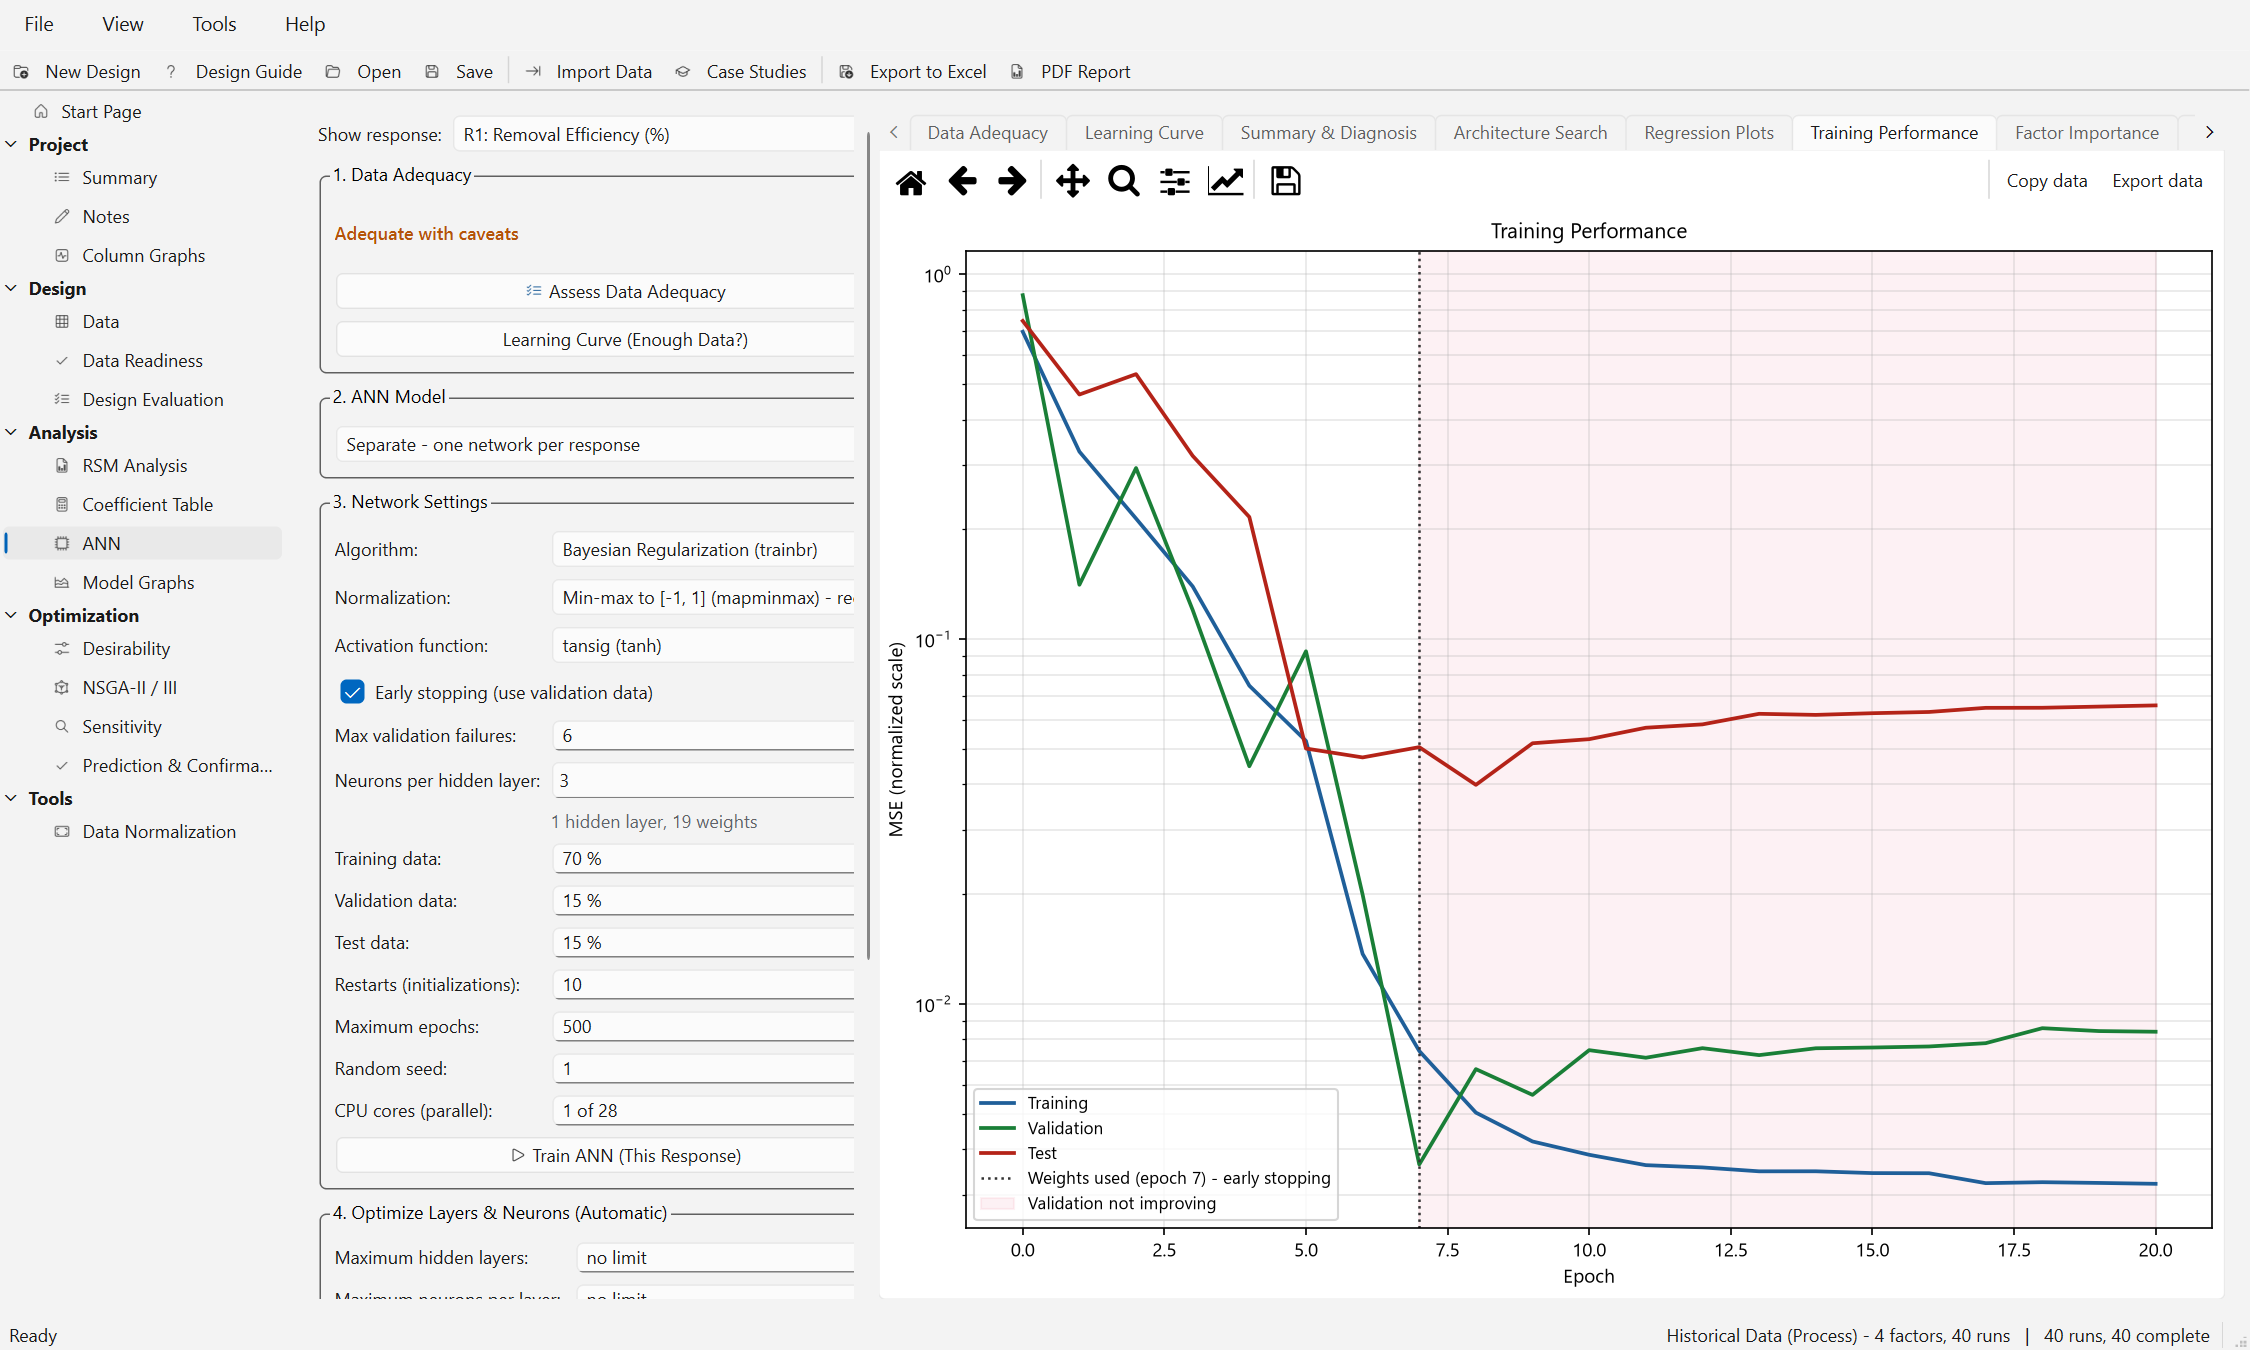
\includegraphics[width=\linewidth]{ann_performance.png}
\caption{\ui{Training Performance} of the 4-3-1 network: the weights of epoch 7 (lowest validation error) are used;
the shaded band shows the epochs without validation improvement.}
\label{fig:ch07-performance}
\end{figure}

\paragraph{Factor Importance.} The relative importance of each factor follows Garson's method as described by
\citet{goh1995}, extended to several hidden layers. With the absolute input weights of each first-layer neuron
normalized to shares,
\begin{equation}
  S^{(1)}_{hi} = \frac{|W^{(1)}_{hi}|}{\sum_{i'} |W^{(1)}_{hi'}|}, \qquad
  S^{(l)} = \bar{A}^{(l)} S^{(l-1)}, \quad \bar{A}^{(l)}_{hg} = \frac{|W^{(l)}_{hg}|}{\sum_{g'}|W^{(l)}_{hg'}|},
  \label{eq:ch07-garson1}
\end{equation}
and $v_h$ the weights from the last hidden layer to the output shown, the importance of input $i$ is
\begin{equation}
  I_i = \sum_{h} \frac{|v_h|}{\sum_{h'}|v_{h'}|}\, S^{(L)}_{hi}. \label{eq:ch07-garson2}
\end{equation}
For one hidden layer this is the classic Garson formula; for more layers (``Garson extended to multiple hidden
layers'') each input's share is passed through every layer in proportion to the absolute weights. The values of
the one-hot columns of a categorical factor are added, and the result is scaled to 100~\%. For the dye network the
order is pH 68.2~\%, Initial Concentration 13.3~\%, Contact Time 11.1~\% and Adsorbent Dose 7.4~\%
(Figure~\ref{fig:ch07-importance}), consistent with the strong pH optimum of this system. Garson's method uses only
weight magnitudes: it shows neither the direction of an effect nor whether it is linear, and it becomes
unreliable when factors are correlated. Use the model graphs or the sensitivity study for the shape of the
effects.

\begin{figure}[htbp]
\centering
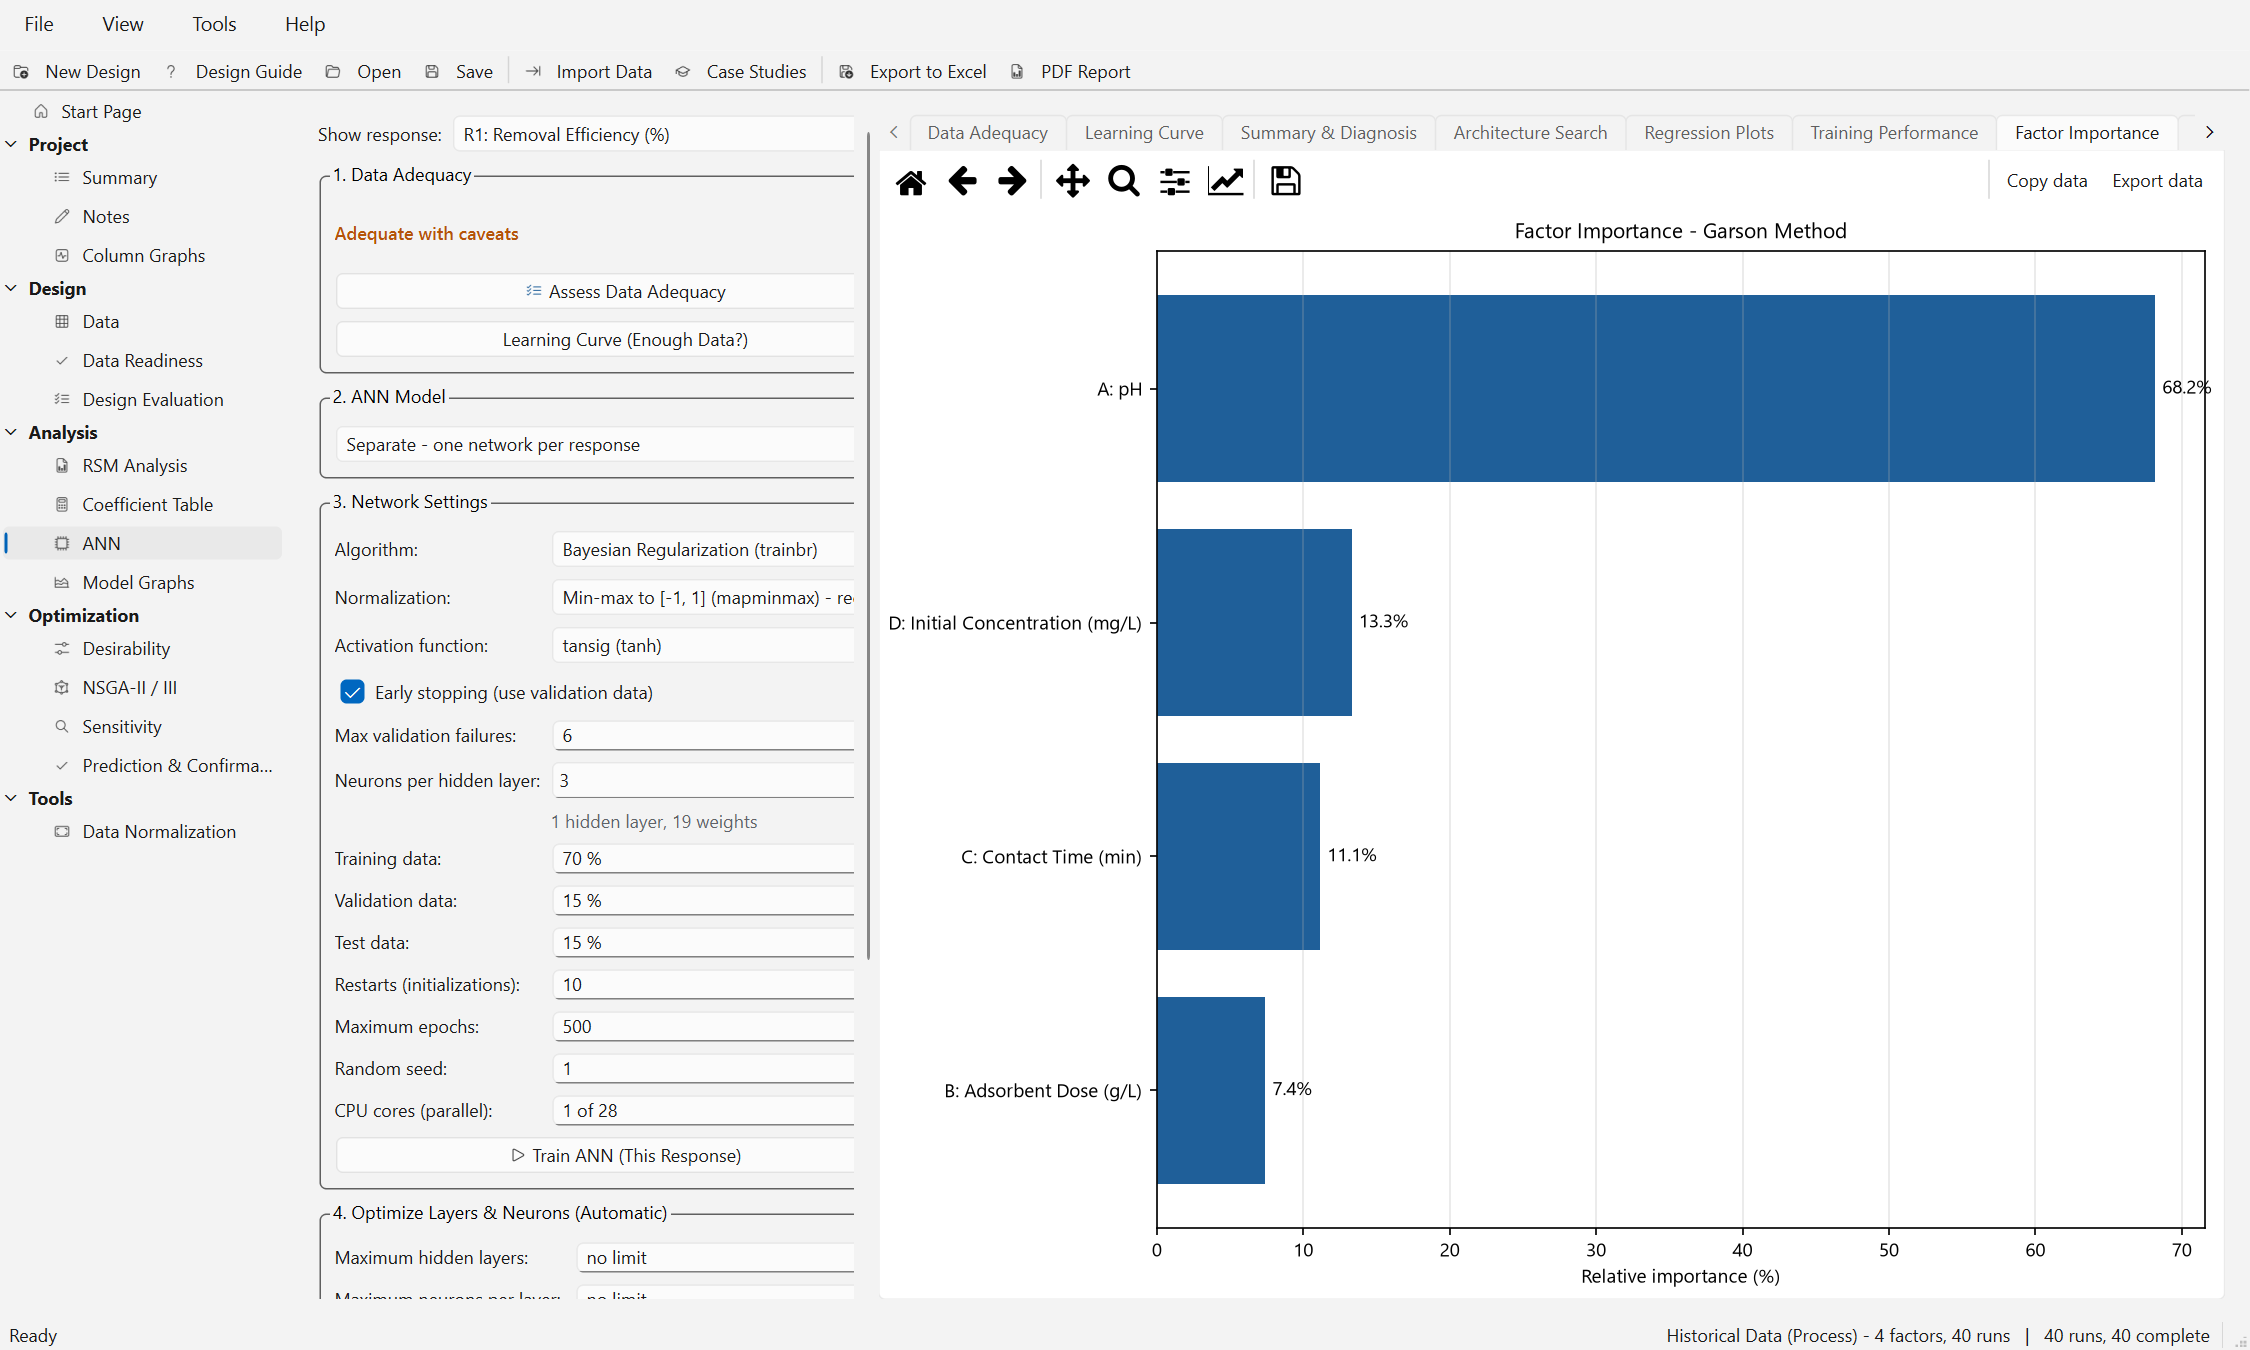
\includegraphics[width=\linewidth]{ann_importance.png}
\caption{\ui{Factor Importance} (Garson method) of the 4-3-1 network.}
\label{fig:ch07-importance}
\end{figure}

\paragraph{RSM vs ANN.} The left panel plots predicted against actual values for both models on all runs (RSM as
squares, ANN as dots, each with its $R^2$); the right panel shows the residual (actual $-$ predicted) per run in
standard order. In the dye case (Figure~\ref{fig:ch07-rsmann}) RSM reaches $R^2$ 0.8769 with residuals up to about
$+16$ and even a negative prediction, while the ANN reaches 0.9614 and stays within about $\pm 6$ except for one
run. Both values are on the data used for fitting (the RSM on all runs); judge predictive accuracy by the
cross-validated values of the search.

\begin{figure}[htbp]
\centering
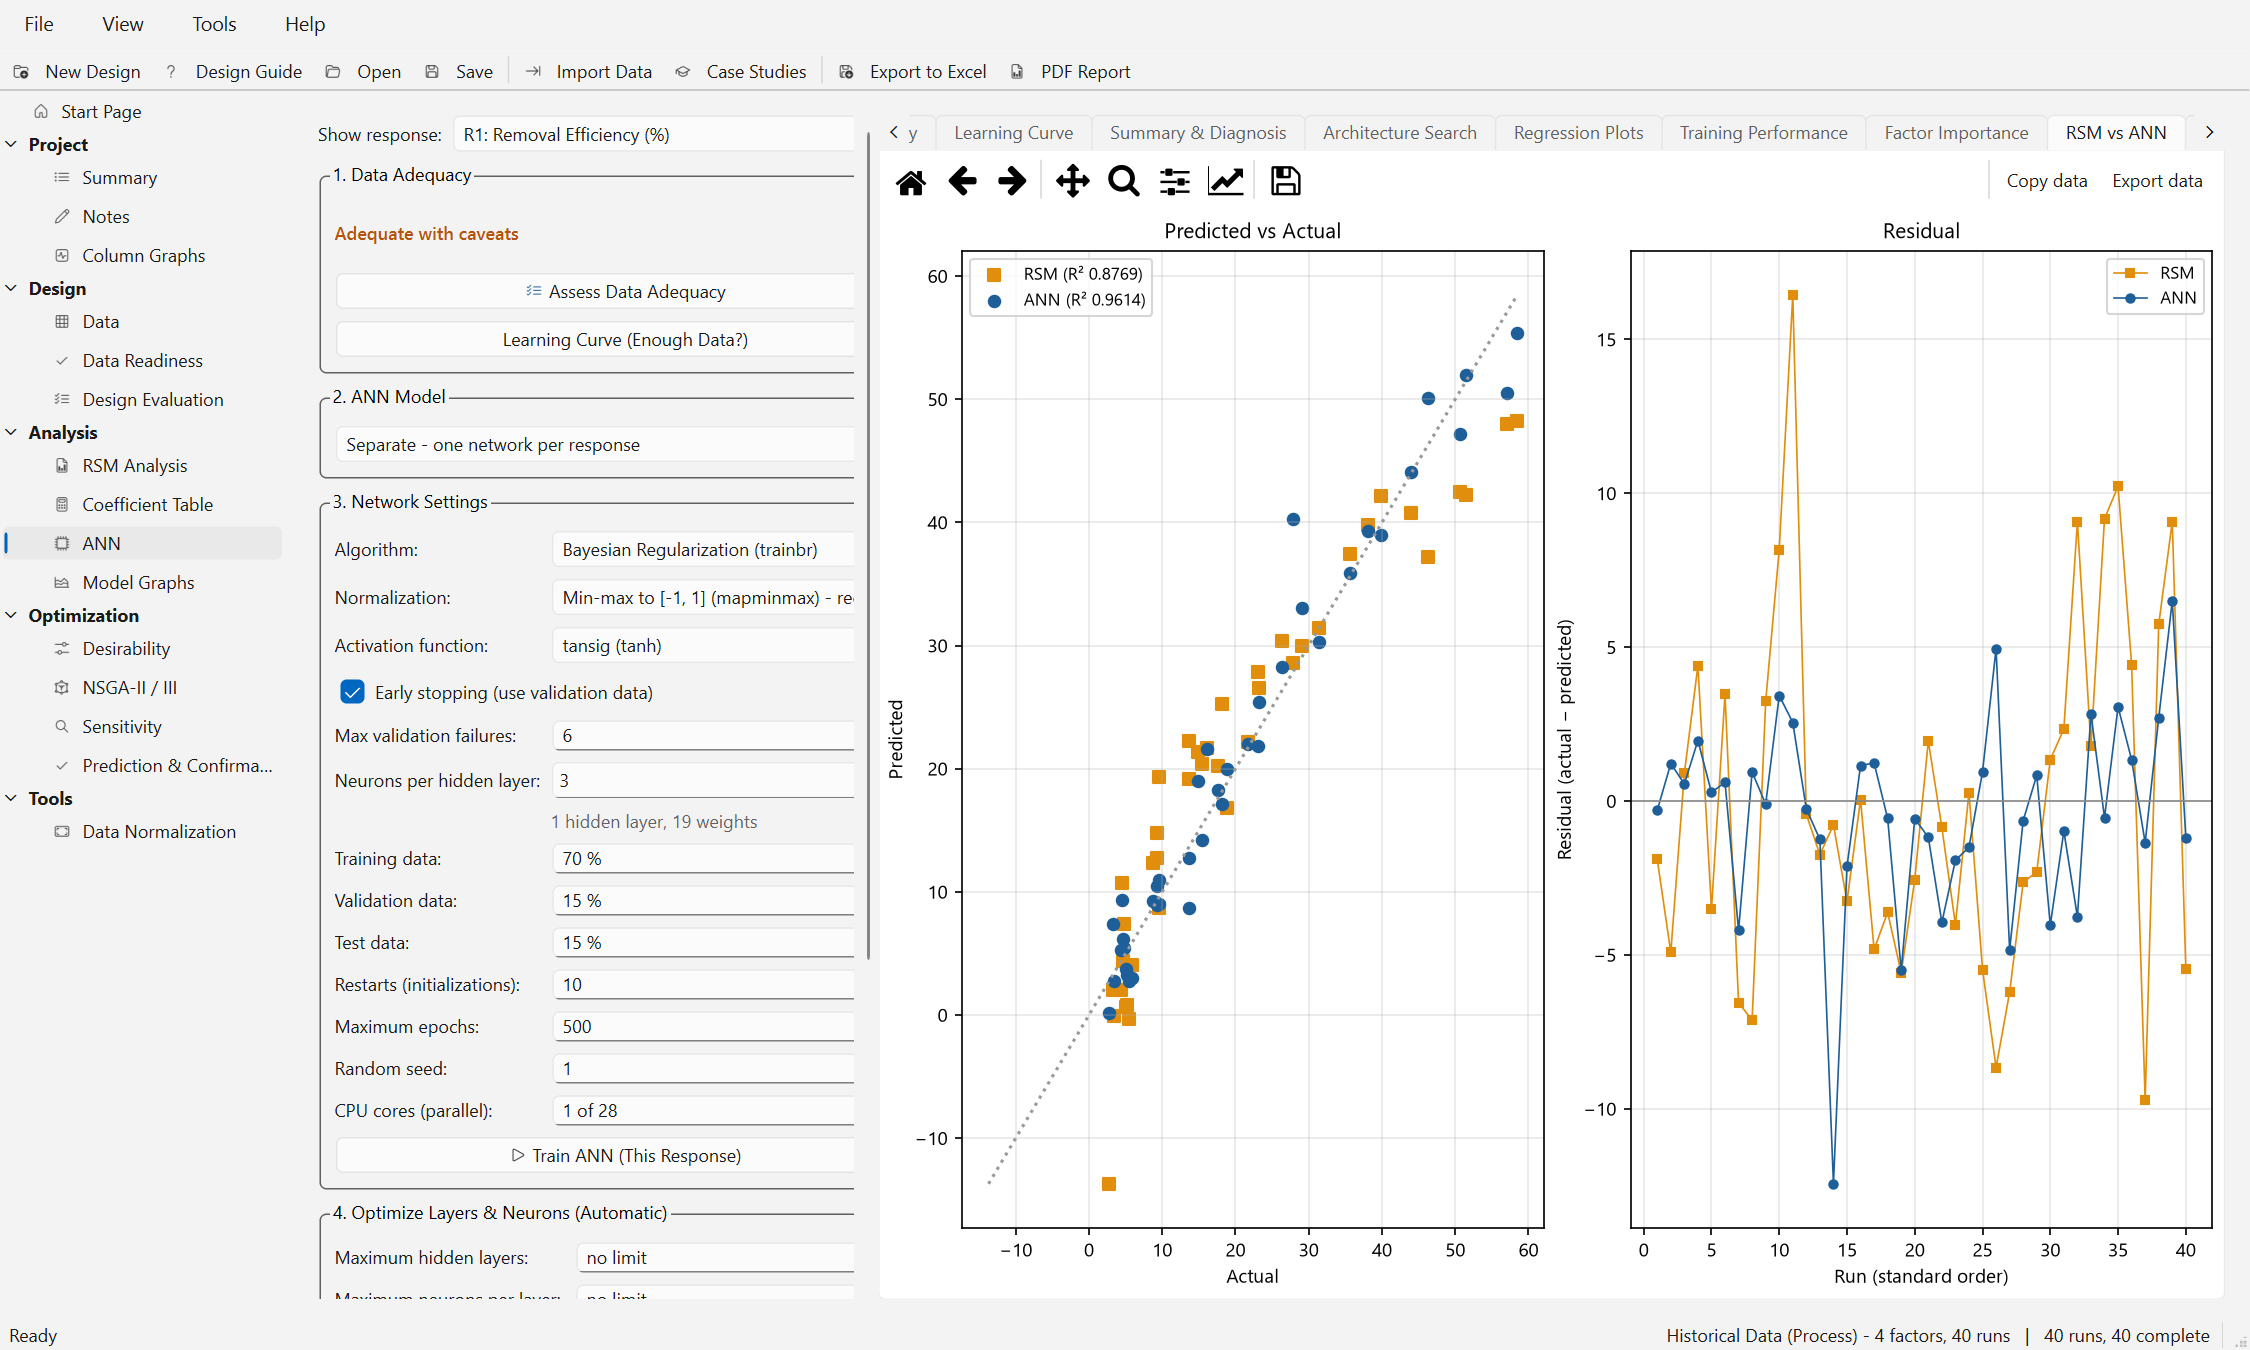
\includegraphics[width=\linewidth]{ann_rsm_vs_ann.png}
\caption{\ui{RSM vs ANN} tab for the dye case: predicted against actual values and residuals per run.}
\label{fig:ch07-rsmann}
\end{figure}

\paragraph{Network Diagram.} Inputs on the left, one column per hidden layer (``Hidden $i$ ($n$ neurons, tansig)''),
linear outputs on the right (Figure~\ref{fig:ch07-diagram}). Blue lines are positive weights, red lines negative;
thickness and opacity grow with $|w|$. In a combined network the output shown is highlighted.

\begin{figure}[htbp]
\centering
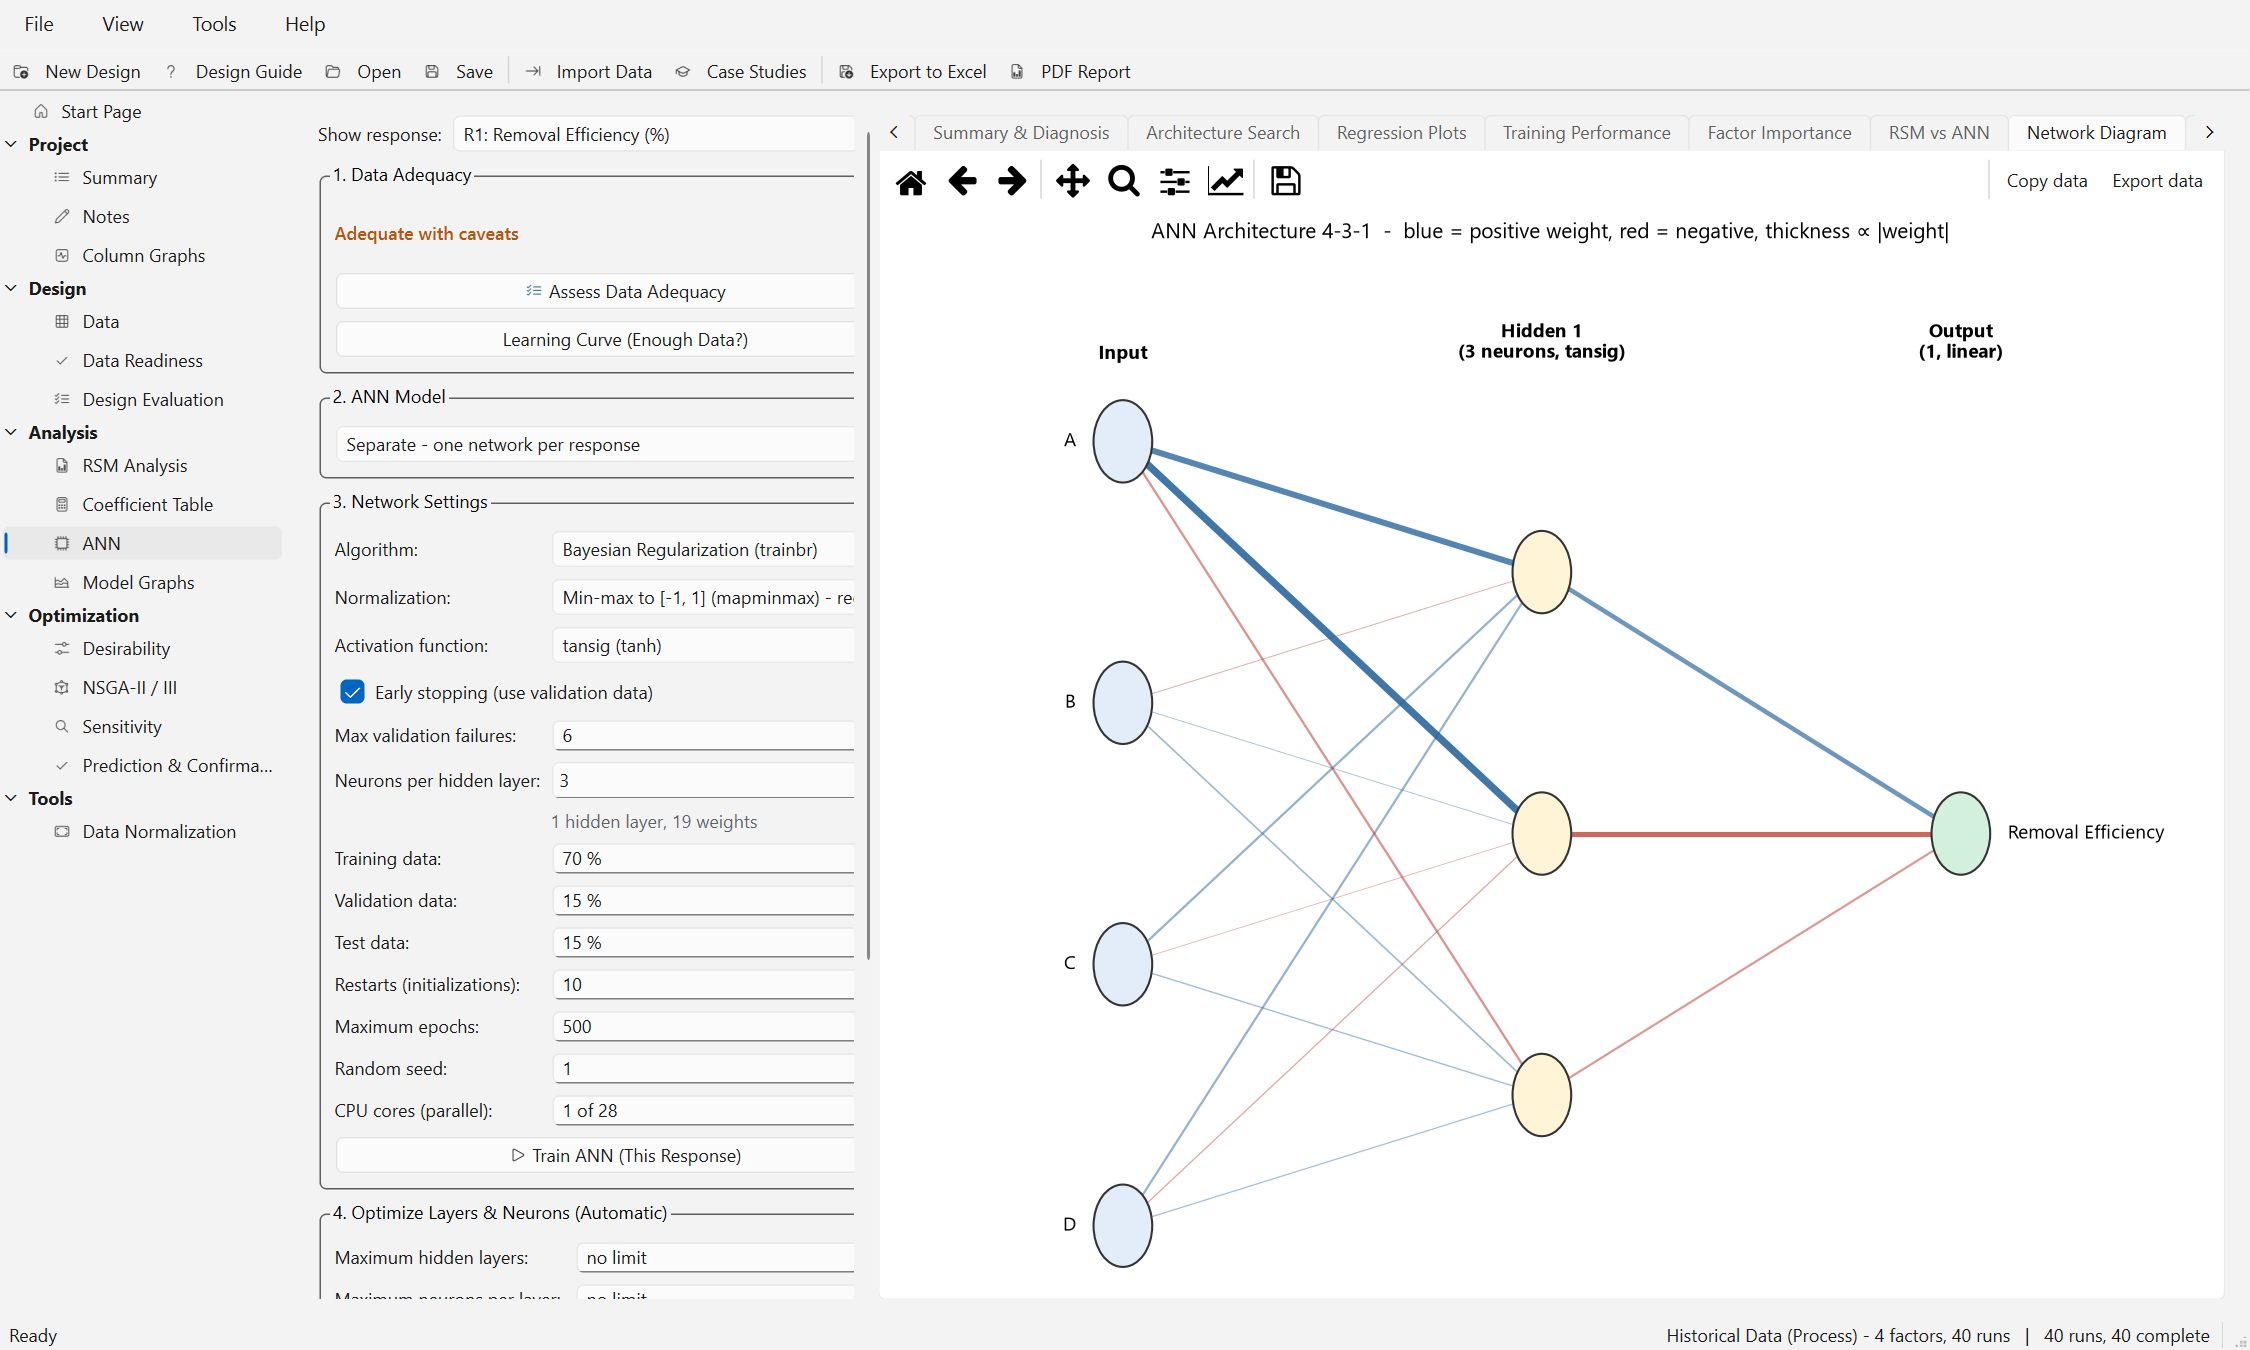
\includegraphics[width=\linewidth]{ann_diagram.png}
\caption{\ui{Network Diagram} of the 4-3-1 network.}
\label{fig:ch07-diagram}
\end{figure}

\paragraph{Weights \& Biases.} Tables of the input-to-hidden weights and biases (IW, b1), the weights between hidden
layers, the hidden-to-output weights and output biases (LW, b output), and the normalization parameters (min and
max of the training and validation runs, offset, scale, base) of every input and output
(Figure~\ref{fig:ch07-weights}). With Eqs.~\eqref{eq:ch07-input}--\eqref{eq:ch07-output} and
\eqref{eq:ch07-normalize} these numbers reproduce the network outside REGEN: code the factors, normalize them,
apply each layer, and convert the output back to response units. The note below the tables states this recipe.

\begin{figure}[htbp]
\centering
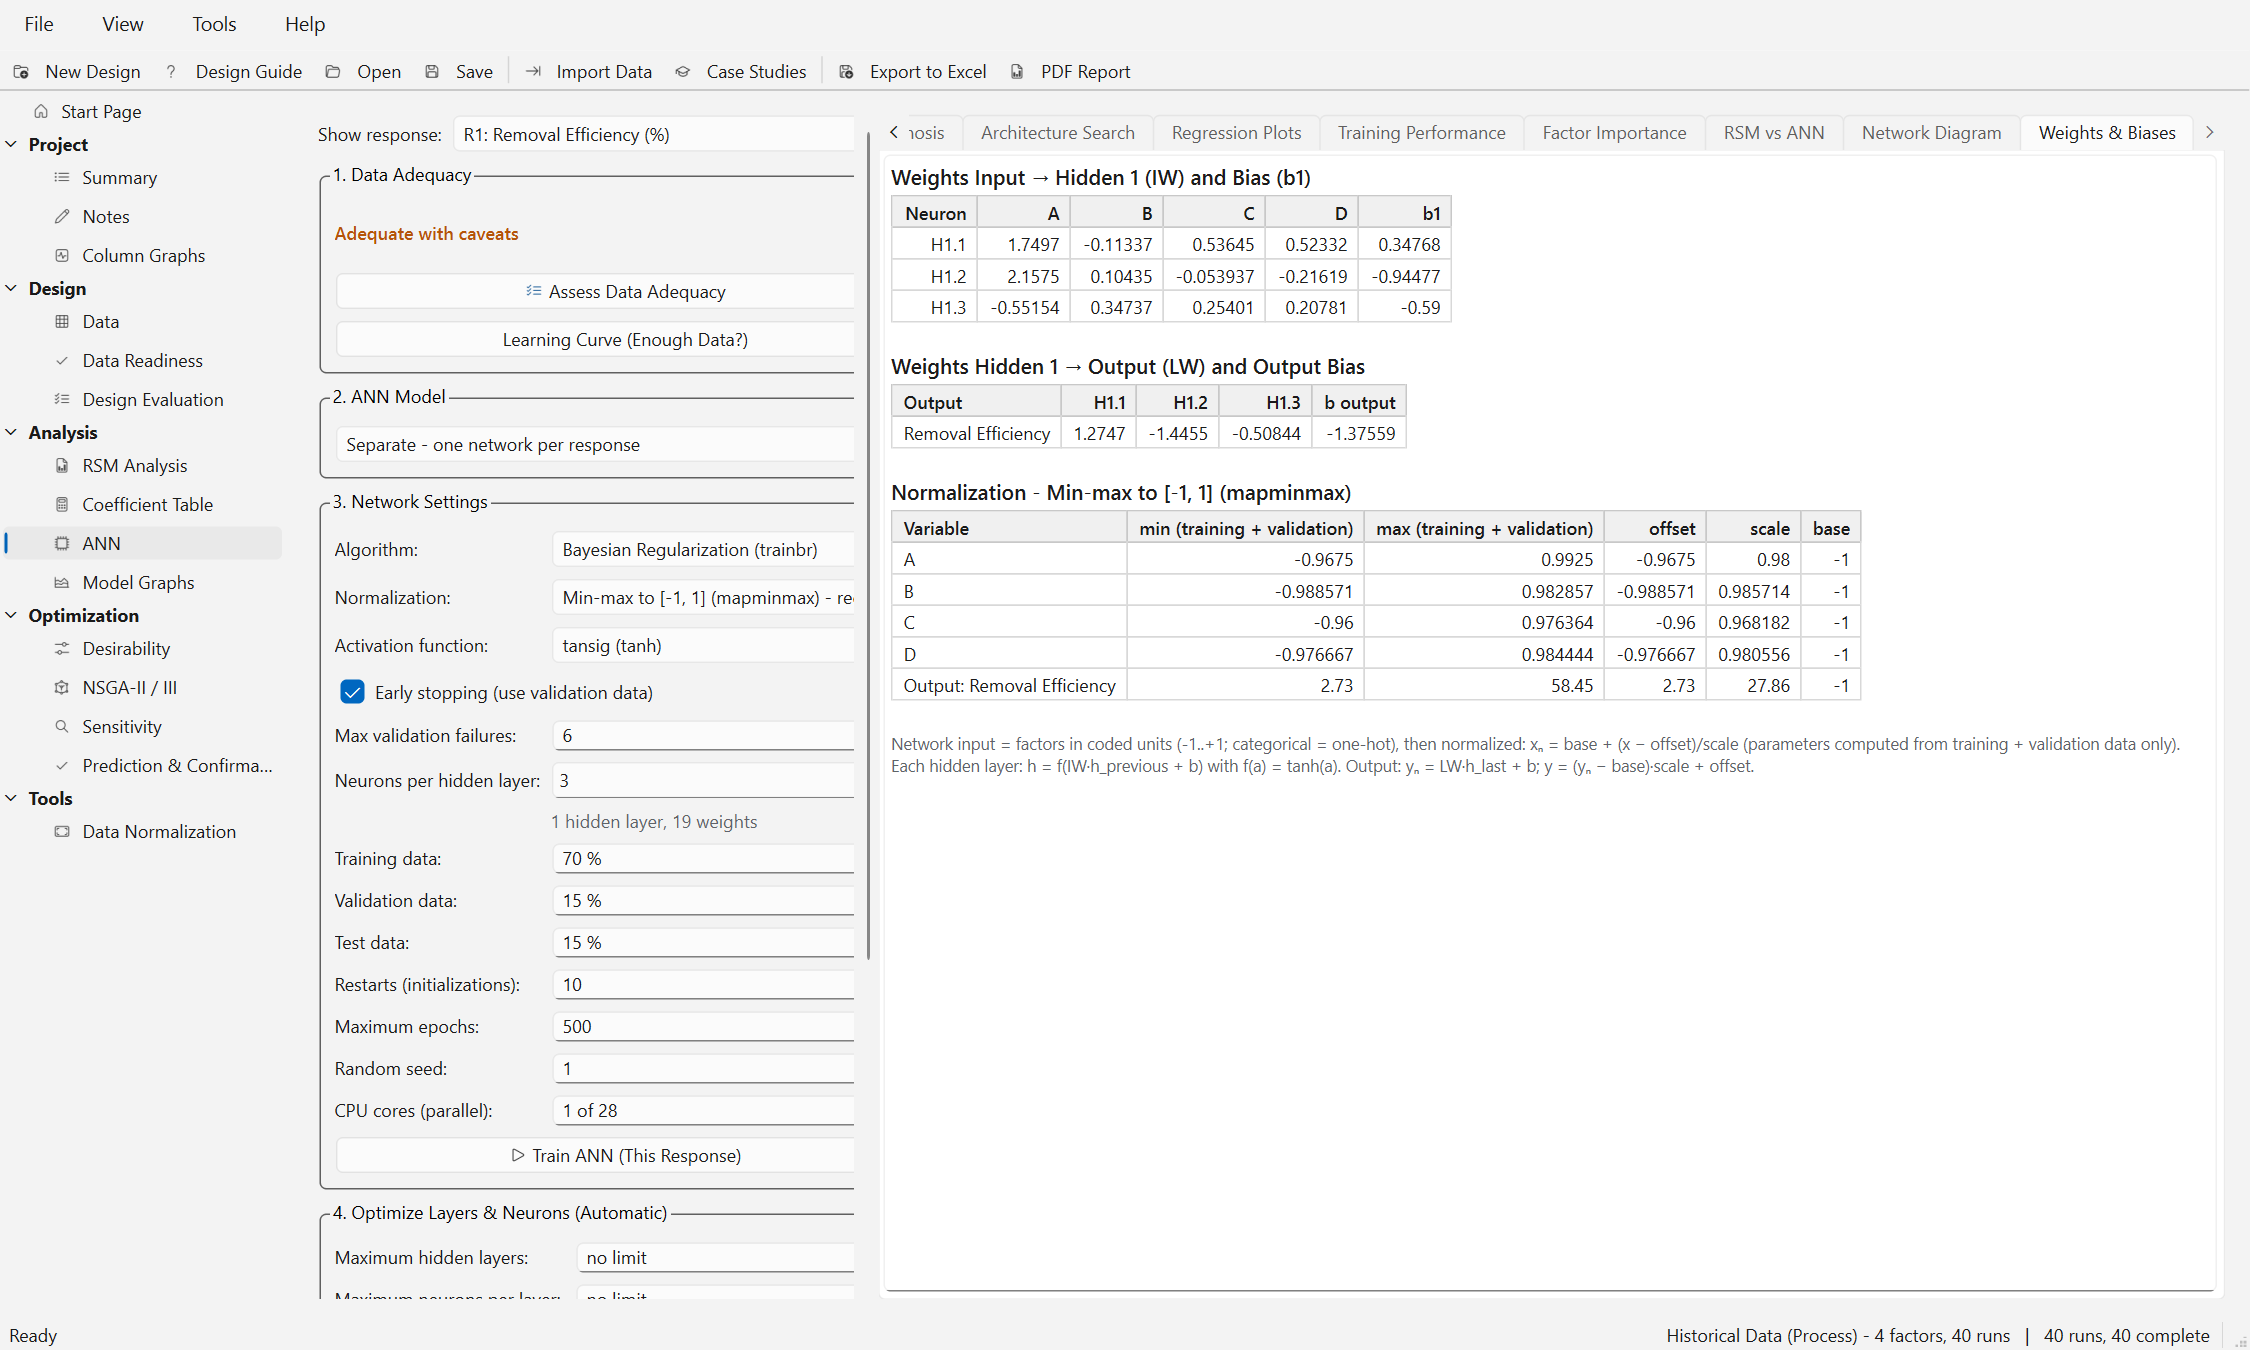
\includegraphics[width=\linewidth]{ann_weights.png}
\caption{\ui{Weights \& Biases} of the 4-3-1 network with the normalization parameters.}
\label{fig:ch07-weights}
\end{figure}

\paragraph{Data export.} Every plot of the page has \ui{Copy data} and \ui{Export data\dots} in its toolbar
(\ui{Copy plot data} and \ui{Export plot data\dots} on right-click); the data behind each panel go to the clipboard,
an Excel workbook or a CSV file. The report tabs (\ui{Data Adequacy}, \ui{Learning Curve}, \ui{Summary \&
Diagnosis}, \ui{Architecture Search}, \ui{Weights \& Biases}) offer \ui{Export all tables\dots} on right-click,
which writes each table to its own sheet.

\section{Using the network in other pages}\label{sec:ch07-use}

The check box \ui{Use this response's ANN for graphs, optimization, NSGA-II \& prediction} is available once the
shown response has a network. When it is ticked, the network replaces the RSM model of that response on the
\ui{Model Graphs}, \ui{Desirability}, \ui{NSGA-II / III}, \ui{Sensitivity} and \ui{Prediction \& Confirmation}
pages. The same choice is made per response in the \ui{Model} column of the desirability and NSGA tables. A network
gives point predictions only: confidence and prediction intervals are not available (Chapter~\ref{chap:10}), and the
confirmation rule for an ANN is a tolerance on the error.

Select the ANN only when it predicts new data better than RSM, judged by the cross-validated test $R^2$ of the
search against the RSM test $R^2$ on the same folds and the RSM Predicted $R^2$. When an optimization depends on
the choice of model, the comparison of the RSM and ANN Pareto fronts (check~D, Chapter~\ref{chap:8}) shows how much, and
confirmation runs settle the question.

\section{Parallel processing}\label{sec:ch07-parallel}

Training many networks is the slowest part of REGEN. \ui{CPU cores (parallel):} sets the number of processor cores
used (default: all logical cores but one, so the computer stays responsive). The work is divided into independent
jobs:
\begin{itemize}
  \item in the architecture search, every combination of candidate network, data split and restart is one job.
    When there are more cores than jobs per candidate, the next few neuron counts (at most patience $+2$) are
    evaluated together; they are recorded in order and candidates after a stop are discarded, so the decisions are
    the same as on one core;
  \item in the learning curve, every point of every repeat is one job;
  \item in \ui{Train ANN}, the restarts run in parallel when the work is large enough to pay for starting the
    worker processes (estimated as training runs $\times$ weights $\times$ outputs $\times$ epochs $\times$
    restarts $\ge 3\times10^7$) or when the workers are already running;
  \item \ui{Optimize All Responses (One Click)} searches several responses at the same time when at least 16 cores
    are selected (one response per 8 cores).
\end{itemize}
Each job has its own random generator derived from the seed, so the results do not depend on the number of
cores; only the time does. The worker processes use one thread each and are closed after 90~s without work. The
work runs in the background so the window stays responsive; \ui{Stop} cancels it (the status line shows
``Stopping\dots''). For data sets with more than 5000 runs, the final training uses at most $\max(3,
\text{cores})$ restarts (``large data (\dots{} runs): restarts limited to \dots''). If a worker process fails, for
example for lack of memory, the message is ``A parallel process stopped unexpectedly (possibly not enough
memory).''; reduce the number of cores or the network size.

\section{Saving results}\label{sec:ch07-saving}

\menupath{File $\rightarrow$ Save} stores in the project file every trained network (weights, normalization, data
split, settings, training history, single-split and cross-validated diagnosis), the choice between RSM and ANN for
each response, the architecture search results and the learning curves. When the project is opened again, the
tabs show the saved results without retraining; the data adequacy report is recomputed. A search result larger
than about 5 million characters (very large searches) is not saved; the network itself is always saved. Changing
the data after a search does not update the saved results: repeat the search and the learning curve after adding
or excluding runs.

\section{Practical advice and limitations}\label{sec:ch07-advice}

\begin{itemize}
  \item An ANN is a data-hungry model. With fewer than about 20--30 runs, a well-chosen RSM model is usually more
    reliable, and the search will often show that RSM predicts new data as well as the ANN. Designed experiments
    with few runs (a Box-Behnken design with 17 runs) rarely support an ANN.
  \item Always judge an ANN by data it has not seen: the cross-validated test $R^2$ of the search, the learning
    curve, and finally confirmation runs (Chapter~\ref{chap:10}). Training $R^2$ alone says nothing about prediction.
  \item The random seed changes the data split and the initial weights. With small data sets, results can change
    noticeably with the seed; this is another reason to rely on cross-validation.
  \item An ANN extrapolates poorly. Predictions outside the region covered by the runs (including gaps inside it)
    can be far off even when the test $R^2$ is high.
  \item The network has no confidence or prediction intervals in REGEN. Its uncertainty is summarized only by the
    cross-validated test RMSE.
  \item The noise rules of the diagnosis need replicated runs. Without them, overfitting can only be detected from
    the error on new data.
\end{itemize}

% Chapter 8: Optimization (desirability, NSGA-II / NSGA-III, checks C and D)
\chapter{Optimization}\label{chap:8}
\label{ch:08}

The \ui{Optimization} group of the navigation tree contains four pages: \ui{Desirability}, \ui{NSGA-II / III},
\ui{Sensitivity} and \ui{Prediction \& Confirmation}. This chapter describes the first two. The \ui{Sensitivity}
page is the subject of Chapter~\ref{chap:9} and the \ui{Prediction \& Confirmation} page of Chapter~\ref{chap:10}.

Both optimization pages work on fitted models, never on the raw data. For every response you choose the model in a
\ui{Model} column: \ui{RSM} (the polynomial, GLM or split-plot model of the RSM Analysis page, Chapter~\ref{chap:5}) or
\ui{ANN} (the network trained on the ANN page, Chapter~\ref{chap:7}). The \ui{ANN} item is disabled until a network exists for
that response; its tooltip then shows the network architecture with its accuracy (``cross-validation Q2'' from
the architecture search, if one was run, and ``test R2 (single split)''), and the tooltip of \ui{RSM} shows the
predicted $R^2$ of the polynomial. The choice is stored in the project and is shared by all pages: changing the model on the
\ui{Desirability} page also changes it on the \ui{NSGA-II / III} page, in the model graphs and on the prediction
page.

The two pages answer different questions.
\begin{itemize}
  \item \textbf{Desirability} turns several responses into one score $D$ between 0 and 1 and finds the factor
        settings with the highest score. You state in advance how good each response must be and how important it
        is. The result is a short list of settings.
  \item \textbf{NSGA-II / III} keeps the objectives separate and returns the whole set of best compromises (the
        Pareto front). You see the trade-off first and choose afterwards, with help from TOPSIS and the knee point.
        The page also contains two of the diagnostic checks of REGEN: check~C (convergence and population size of
        the genetic algorithm) and check~D (comparison of the fronts obtained with the ANN and the RSM models).
\end{itemize}

% ======================================================================================================
\section{Desirability optimization}
\label{sec:ch08-desirability}

\subsection{Purpose}
The \ui{Desirability} page (page title \ui{Desirability Optimization}) finds factor settings that satisfy several
response goals at the same time, for example ``maximize yield and purity, keep cost below a limit''. Each response
is rated by an individual desirability $d_i\in[0,1]$, and the settings with the highest overall desirability $D$
are reported \citep{derringer1980,myers2016}.

\subsection{How to use}
\begin{enumerate}
  \item Fit the models first (RSM Analysis, and ANN if you want to use networks). A response without a model is
        skipped with the message \ui{Skipped responses without a model: \dots}.
  \item Open \ui{Desirability} in the navigation tree. The upper group \ui{Optimization Criteria} lists one row
        per factor, one row per response and, when factor standard deviations have been entered (Chapter~\ref{chap:4},
        \ui{Factor \& Response Info\dots}), one \ui{POE} row per response.
  \item In the factor rows, narrow the \ui{Lower Limit} and \ui{Upper Limit} if the search should stay inside a
        smaller region. The limits are in actual units.
  \item In each response row choose a \ui{Goal}, edit the limits (and the \ui{Target} for the goal
        \ui{Target}), and set \ui{Shape}, \ui{Importance} and \ui{Model}.
  \item Click \ui{Run Optimization}. The solutions appear in the group \ui{Solutions (Sorted by Desirability)},
        and the bar chart on the right shows the individual and combined desirability of the selected row.
  \item Select a row and click \ui{Send Selected Solution to Prediction} to obtain confidence and prediction
        intervals and to plan confirmation runs (Chapter~\ref{chap:10}).
\end{enumerate}
\ui{Reset Limits to Data} refills all limits and targets with their defaults. The criteria are saved in the project,
and the \ui{NSGA-II / III} page takes its factor limits, goals and targets from them.

\subsection{Options}
Table~\ref{tab:ch08-desir-options} lists the columns of the criteria table.

\begin{table}[htbp]
\centering
\small
\caption{Columns of the \ui{Optimization Criteria} table on the \ui{Desirability} page.}
\label{tab:ch08-desir-options}
\begin{tabularx}{\linewidth}{@{}>{\raggedright\arraybackslash}p{3.0cm} >{\raggedright\arraybackslash}p{3.4cm} >{\raggedright\arraybackslash}p{2.3cm} >{\raggedright\arraybackslash}X@{}}
\toprule
Column & Values & Default & Meaning \\
\midrule
\ui{Goal} (factor) & \ui{In range} (numeric), \ui{All levels} (categoric) & fixed & Numeric factors are searched
between their limits; every level combination of the categoric factors is optimized separately. \\
\ui{Lower Limit}, \ui{Upper Limit} (factor) & numbers in actual units & factor low and high & Search region. \\
\ui{Goal} (response) & \ui{None}, \ui{Maximize}, \ui{Minimize}, \ui{Target}, \ui{In range} & \ui{None} & \ui{None}
leaves the response out of $D$. \\
\ui{Lower Limit}, \ui{Upper Limit} (response) & numbers & data minimum and maximum & $L$ and $U$ in
Eqs.~\eqref{eq:ch08-dmax}--\eqref{eq:ch08-drange}. For a binomial response the proportion (count / trials) is
used. \\
\ui{Target} & number between the limits & midpoint of the data range & $T$ for the goal \ui{Target}; ignored for the
other goals. \\
\ui{Shape} & 0.10--10.00, step 0.1 & 1.00 & Shape exponent $s$ of the desirability ramp (1 = linear). \\
\ui{Importance} & \ui{+} \dots\ \ui{+++++} (1--5) & \ui{+++} (3) & Weight $r_i$ in the geometric mean
\eqref{eq:ch08-D}. \\
\ui{Model} & \ui{RSM}, \ui{ANN} & \ui{RSM} & Model used to predict the response (project-wide choice). POE rows show
\ui{follows response}. \\
\bottomrule
\end{tabularx}
\end{table}

For a \ui{POE} row the default limits are 0 and the largest POE value over the design points; the usual goal is
\ui{Minimize}, which favors settings where the response is insensitive to small variations of the factors.

\subsection{Output and how to read it}
The solutions table has the columns \ui{No}, the factors (actual units), all responses (predicted with the model
selected for each response) and \ui{Desirability}. At most 20 solutions are listed; row~1, the best, is shaded
green. Solutions that lie within 0.03 coded units of a better one are removed, so the rows are genuinely different
settings. When all starts converge to the same point you get a single row; several rows with nearly the same $D$
indicate a flat optimum, where you may choose the most convenient setting.

The bar chart (title \ui{Desirability of solution $k$}) shows each $d_i$ in blue and the combined $D$ in green.
A response with $d_i$ close to 0 is the bottleneck; relaxing its limits or lowering the importance of the other
responses changes the compromise most.

Messages (title \ui{Optimization}):
\begin{itemize}
  \item \ui{Some limits are not numbers.}, \ui{Invalid limits for factor \dots}, \ui{Limits for response \dots:
        lower must be < upper.}, \ui{The target for \dots\ must be between the limits.}: correct the table.
  \item \ui{Choose a goal (Maximize/Minimize/Target/In range) for at least one response whose model is
        available.}: no response is active.
  \item \ui{The component limits do not allow the mixture to sum to the total.}: for mixtures, the lower limits sum
        to more than the total (or the upper limits to less).
  \item \ui{No point satisfies all limits and constraints.}: none of the random points satisfies the linear
        constraints of the design together with the factor limits; widen the limits.
\end{itemize}

\subsection{Theory as implemented}
Let $y_i(\mathbf x)$ be the prediction of response $i$ at the factor setting $\mathbf x$ (coded units), $L_i$ and
$U_i$ its limits, $T_i$ its target and $s_i$ its shape exponent. REGEN uses the desirability functions of
\citet{derringer1980}:
\begin{align}
\text{Maximize:}\quad & d_i=\left[\operatorname{clip}\!\left(\frac{y_i-L_i}{U_i-L_i},0,1\right)\right]^{s_i},
\label{eq:ch08-dmax}\\
\text{Minimize:}\quad & d_i=\left[\operatorname{clip}\!\left(\frac{U_i-y_i}{U_i-L_i},0,1\right)\right]^{s_i},
\label{eq:ch08-dmin}\\
\text{Target:}\quad & d_i=\begin{cases}
\left(\dfrac{y_i-L_i}{T_i-L_i}\right)^{s_i}, & L_i\le y_i\le T_i,\\[2ex]
\left(\dfrac{U_i-y_i}{U_i-T_i}\right)^{s_i}, & T_i< y_i\le U_i,\\[1ex]
0, & \text{otherwise,}\end{cases}
\label{eq:ch08-dtarget}\\
\text{In range:}\quad & d_i=\begin{cases}1, & L_i\le y_i\le U_i,\\ 0, & \text{otherwise,}\end{cases}
\label{eq:ch08-drange}
\end{align}
where $\operatorname{clip}(u,0,1)$ limits $u$ to $[0,1]$. With $s_i=1$ the ramp is linear; with $s_i>1$ the
response must come close to the goal before $d_i$ rises; with $s_i<1$ the desirability rises quickly away from the
limit. The original paper allows different exponents on the two sides of a target; REGEN uses the same exponent
on both sides. A prediction that is not a number gives $d_i=0$.

Note the consequence of the clipping in \eqref{eq:ch08-dmax}: once $y_i\ge U_i$ the response is fully desirable,
and the search no longer tries to increase it. With the default limits (data minimum and maximum), maximizing a
response means ``reach at least the best observed value''. If you want the search to go further, raise $U_i$, but
remember that predictions beyond the observed range are extrapolations.

The overall desirability is the importance-weighted geometric mean
\begin{equation}
D(\mathbf x)=\left(\prod_{i} d_i^{\,r_i}\right)^{1/\sum_i r_i}
=\exp\!\left(\frac{\sum_i r_i\ln d_i}{\sum_i r_i}\right),\qquad D=0\ \text{if any}\ d_i=0,
\label{eq:ch08-D}
\end{equation}
with $r_i\in\{1,\dots,5\}$ the importance. Responses with goal \ui{None} are left out. Because $D$ is a geometric
mean, a single unacceptable response ($d_i=0$) makes the whole setting unacceptable.

The search proceeds as follows (\texttt{doe/optimize.py} and \texttt{Project.optimize}):
\begin{enumerate}
  \item The factor limits are converted to coded units (for mixtures intersected with the component bounds).
        Each combination of categoric factor levels is optimized separately with
        $n_\text{starts}=\max(8,\lfloor 30/n_\text{comb}\rfloor)$ starts ($n_\text{comb}$ = number of level
        combinations; 30 starts without categoric factors).
  \item 4000 random points are drawn uniformly in the limits (12\,000 when the design has linear constraints, of
        which the feasible ones are kept, at most 4000). For mixtures the points are drawn uniformly on the simplex
        above the lower bounds and filtered by the upper bounds. The random generator has a fixed seed (0), so the
        same criteria always give the same solutions.
  \item The $n_\text{starts}$ points with the highest $D$ become starting points of a local search: Nelder--Mead
        with bounds (tolerances $10^{-5}$ in $\mathbf x$ and $10^{-8}$ in $D$, at most 2000 iterations) for an
        unconstrained process design, and SLSQP (at most 300 iterations) with the mixture equality
        $\sum x_\text{comp}=1$ and the linear constraints $G\mathbf x\le\mathbf h$ otherwise. An infeasible point
        scores $D=0$, and SLSQP results that are worse than their start are replaced by the start.
  \item All end points are sorted by $D$; points within a Euclidean distance of 0.03 (coded units) of a better
        point are removed; the 20 best are shown.
\end{enumerate}

\textbf{POE criterion.} When standard deviations $\sigma_j$ of the factors have been entered, the propagation of
error of response $i$ is
\begin{equation}
\text{POE}_i(\mathbf x)=\sqrt{\sum_j\left(\frac{\partial y_i}{\partial x_j}\right)^2\sigma_{x,j}^2
+\left(\frac{\partial y}{\partial\eta}\right)^2\sigma^2_\text{resid}},
\label{eq:ch08-poe}
\end{equation}
where $\sigma_{x,j}$ is the factor standard deviation in coded units, the derivatives are central differences with
step $10^{-4}$, $\eta$ is the (possibly transformed) model scale and $\sigma^2_\text{resid}$ is the residual mean
square of the RSM model (for an ANN, its mean squared error on all data). The POE row uses the model of its response.
POE is described in more detail in Chapter~\ref{chap:6}.

\textbf{Limitations.} The optimizer is a multi-start local search. It is reliable for the smooth models of RSM,
but for an ANN with many local optima increase the confidence by comparing with the NSGA front
(Section~\ref{sec:ch08-nsga}). The result is an optimum of the \emph{model}; it must be confirmed by experiments.

\subsection{Example: BBD extraction}
\label{sec:ch08-desir-example}
Case study \ui{Extraction Optimization (Box-Behnken)} (Temperature 60--80~°C, Time 30--90~min,
Concentration 1--3~\%, responses Yield and Purity, both fitted with the quadratic RSM model). Both responses are set
to \ui{Maximize} with lower limits 75 (Yield) and 89 (Purity); the upper limits stay at the data maxima 78.29 and
93.6, shape 1.00, importance \ui{+++}, model \ui{RSM} (Figure~\ref{fig:ch08-desirability}).

\begin{figure}[htbp]
\centering
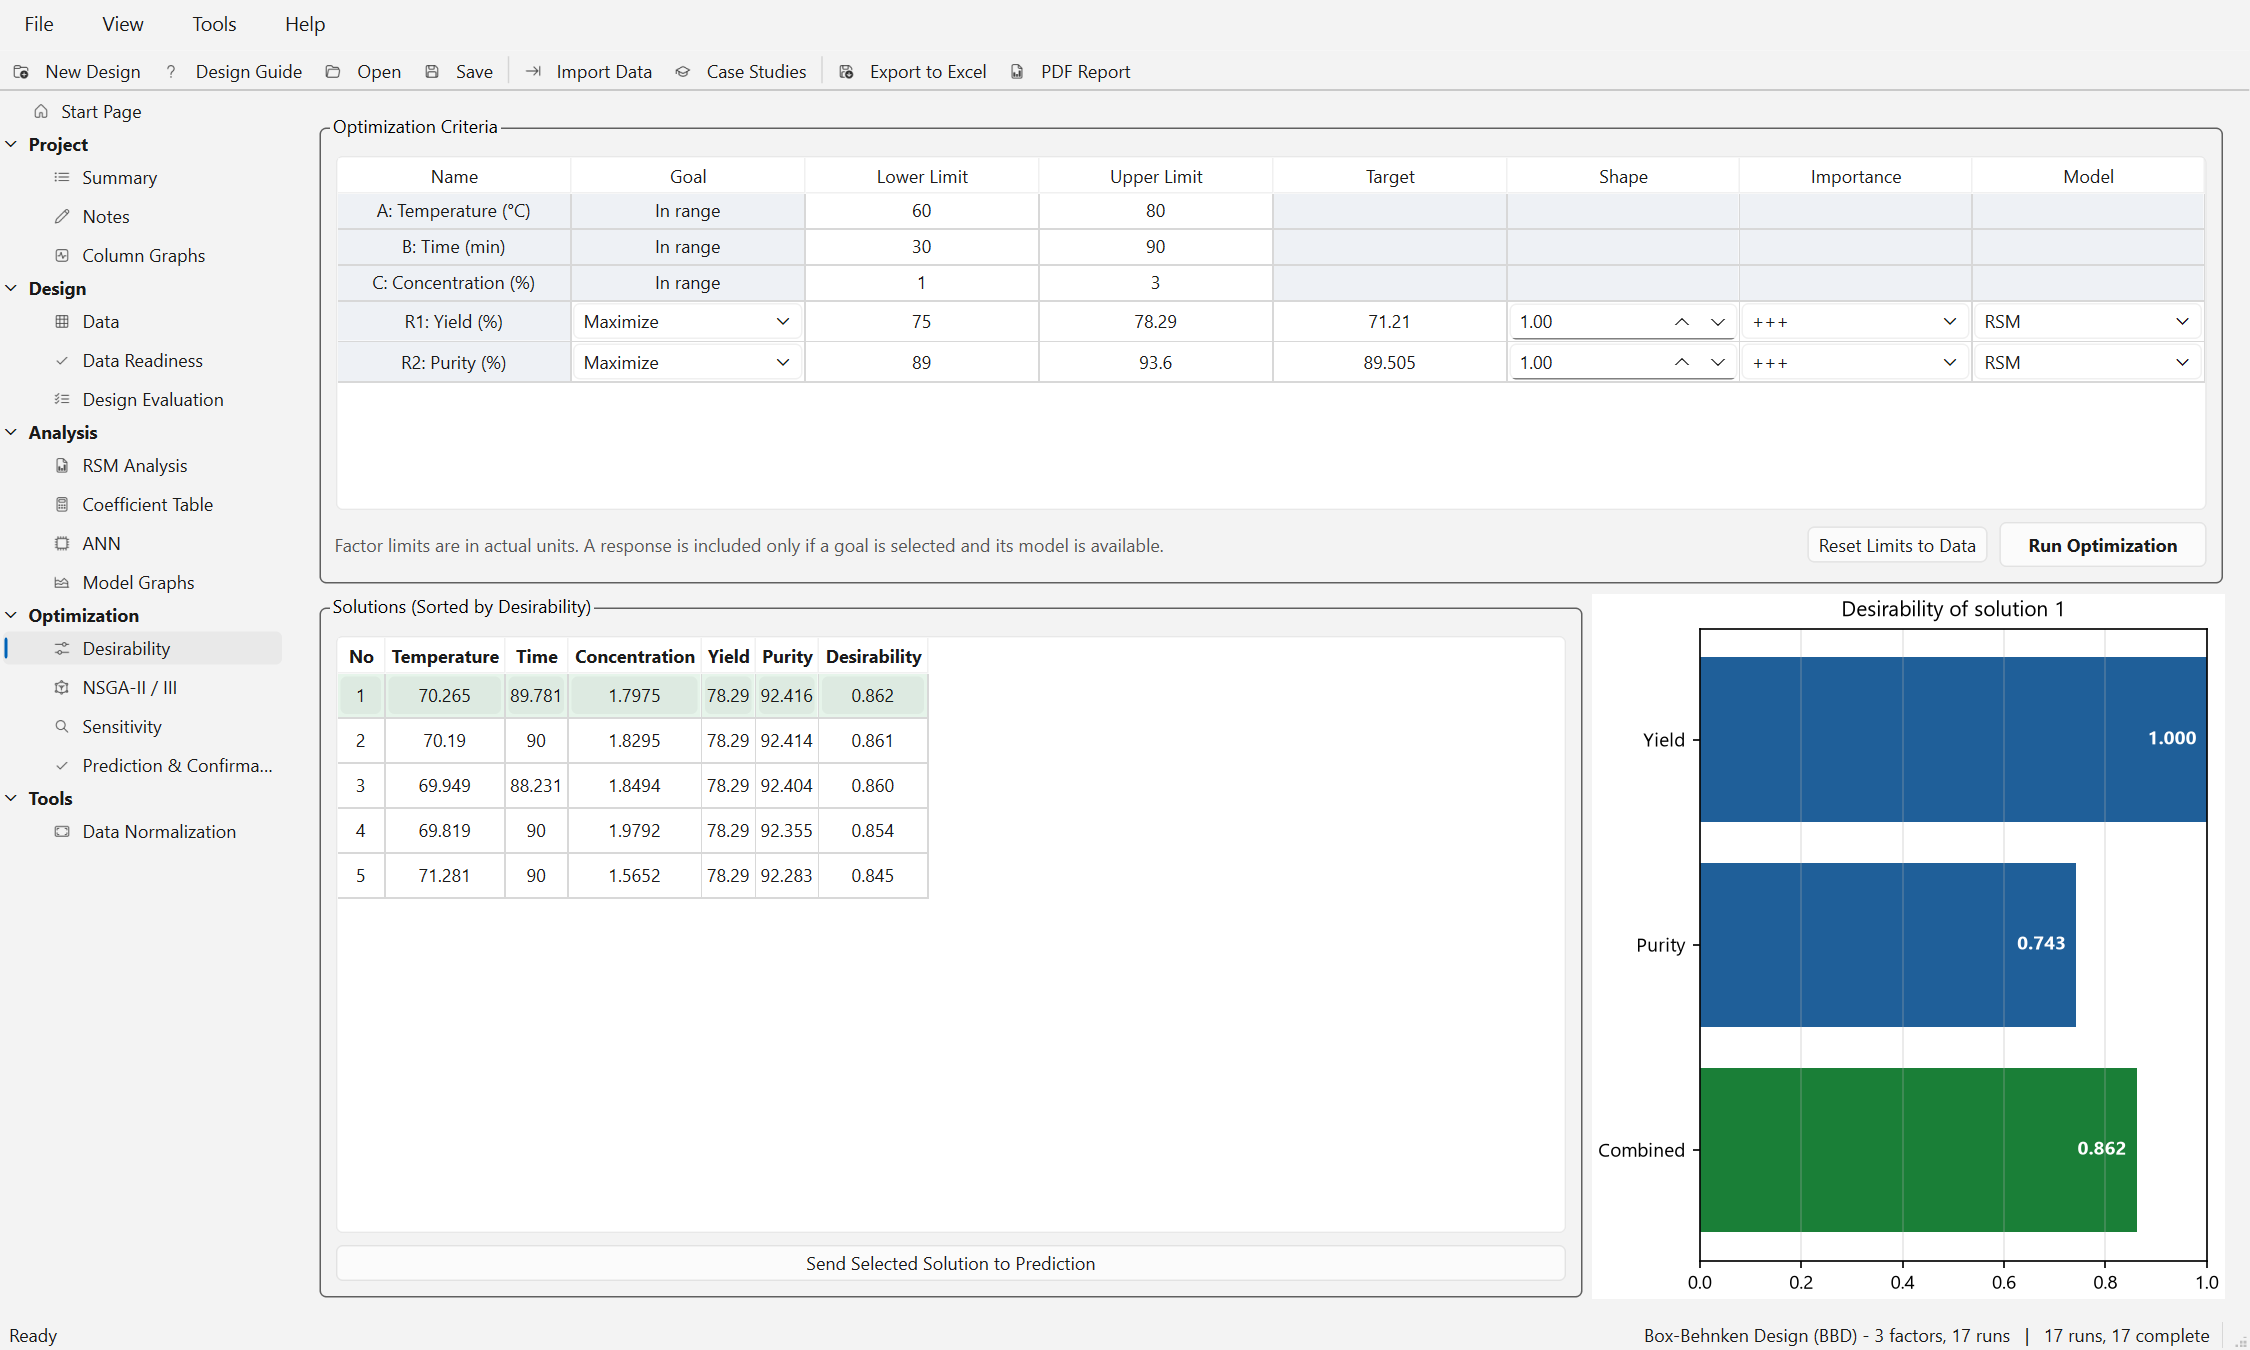
\includegraphics[width=\linewidth]{desirability.png}
\caption{\ui{Desirability} page for the BBD extraction case: Yield and Purity maximized (limits 75--78.29 and
89--93.6). Five distinct solutions; the best, at 70.265~°C, 89.781~min and 1.7975~\%, has $D=0.862$.}
\label{fig:ch08-desirability}
\end{figure}

\ui{Run Optimization} returns five distinct solutions with $D$ between 0.845 and 0.862. The best one is
Temperature 70.265~°C, Time 89.781~min, Concentration 1.7975~\%, with predicted Yield 78.29 and Purity 92.416. The
bar chart shows $d_\text{Yield}=1.000$, $d_\text{Purity}=(92.416-89)/(93.6-89)=0.743$ and
$D=\sqrt{1.000\times0.743}=0.862$ (equal importances, so $D$ is the plain geometric mean).

Yield sits exactly at its upper limit 78.29 in all five rows: once Yield reaches the data maximum its desirability
is 1, so the optimizer spends the remaining freedom on Purity. The five rows differ mainly in Concentration
(1.57--1.98~\%), which shows that the optimum is flat in that direction. The NSGA front below shows that the model
predicts Yield up to about 80.4 for lower Purity.

\textbf{Data export.} Right-click the solutions table for \ui{Copy selected cells}, \ui{Copy entire table (for
Excel)} and \ui{Export table\dots}; right-click the bar chart for \ui{Copy plot data} and \ui{Export plot
data\dots}. The solutions are saved with the project.

% ======================================================================================================
\section{Multi-objective optimization: NSGA-II and NSGA-III}
\label{sec:ch08-nsga}

\subsection{Purpose}
The \ui{NSGA-II / III} page (page title \ui{Multi-objective Optimization (NSGA-II / NSGA-III)}) finds the Pareto
front: the set of factor settings for which no objective can be improved without making another one worse. It is
the right tool when the responses conflict and you want to see the trade-off before deciding
\citep{chapman2014}. A compromise is then picked by TOPSIS \citep{hwang1981} or at the knee of the front.

\subsection{How to use}
\begin{enumerate}
  \item Set the factor limits on the \ui{Desirability} page if the search region should be smaller than the design
        range (the NSGA page uses those limits; the note on the page says ``Factor limits are taken from the
        Desirability page.'').
  \item In the group \ui{Objectives \& Constraints (Select at Least 2 Objectives)} choose for each response the
        \ui{Model} and the \ui{Goal} (\ui{Ignore}, \ui{Maximize}, \ui{Minimize}, \ui{Target}). Goals and targets are
        pre-filled from the \ui{Desirability} page when the goal there is \ui{Maximize}, \ui{Minimize} or
        \ui{Target}.
  \item Optionally enter \ui{Lower limit (constraint)} and \ui{Upper limit (constraint)} for any response (empty
        means no limit). A row with goal \ui{Ignore} and a limit becomes a pure constraint.
  \item Optionally change the \ui{TOPSIS weight} of each objective (default 1).
  \item Check the algorithm parameters (Table~\ref{tab:ch08-nsga-options}) and click \ui{Run Optimization}. The
        progress text reads \ui{generation $g$ of max $G$}; \ui{Stop} ends the run early.
  \item Read the front in the \ui{Graph} tab and the convergence check in the \ui{Convergence \& Adequacy} tab.
        Click \ui{Check Population Size} to complete check~C.
  \item If ANN models exist, click \ui{Compare ANN vs RSM} (check~D, Section~\ref{sec:ch08-checkD}).
  \item Select a row of the solutions table and click \ui{Send Selected Solution to Prediction} (without a selection
        the TOPSIS solution is sent).
\end{enumerate}

\subsection{Options}
\begin{table}[htbp]
\centering
\small
\caption{Settings of the \ui{NSGA-II / III} page.}
\label{tab:ch08-nsga-options}
\begin{tabularx}{\linewidth}{@{}>{\raggedright\arraybackslash}p{3.4cm} >{\raggedright\arraybackslash}p{3.6cm} >{\raggedright\arraybackslash}p{2.2cm} >{\raggedright\arraybackslash}X@{}}
\toprule
Setting & Values & Default & Meaning \\
\midrule
\ui{Model} & \ui{RSM}, \ui{ANN} & \ui{RSM} & Model of each response; POE rows show \ui{RSM + POE} or
\ui{ANN + POE}. \\
\ui{Goal} & \ui{Ignore}, \ui{Maximize}, \ui{Minimize}, \ui{Target} & from Desirability & At least two objectives
are required. \\
\ui{Target} & number & from Desirability & Required for the goal \ui{Target}. \\
\ui{Lower/Upper limit (constraint)} & number or empty & empty & Response constraints, Eq.~\eqref{eq:ch08-cv}. \\
\ui{TOPSIS weight} & positive number & 1 & Weight $w_k$ in TOPSIS, Eq.~\eqref{eq:ch08-topsis}. \\
\ui{Population:} & 20--2000 & 100 & Population size $N$ (rounded up to an even number). \\
\ui{Max generations:} & 10--10\,000 & 300 & Upper limit of the number of generations. \\
\ui{P crossover:} & 0.10--1.00 & 0.90 & Probability $p_c$ that a parent pair is crossed. \\
\ui{$\eta$ crossover:} & 1--100 & 15 & Distribution index $\eta_c$ of SBX. \\
\ui{$\eta$ mutation:} & 1--100 & 20 & Distribution index $\eta_m$ of polynomial mutation. \\
\ui{Seed:} & 0--999\,999 & 1 & Random seed; the same seed gives the same front. \\
\ui{Algorithm:} & \ui{Automatic (NSGA-III for 3 or more objectives)}, \ui{NSGA-II}, \ui{NSGA-III (reference
points)} & Automatic & See Section~\ref{sec:ch08-auto}. \\
\ui{Stop automatically on convergence} & on/off & on & Window stopping rule of check~C. \\
\ui{tolerance:} & 0.001--5.000~\% & 0.100~\% & Tolerance $\tau_0$ of the hypervolume gain. \\
\ui{within} & 5--500 generations & 20 & Window length $w$. \\
\bottomrule
\end{tabularx}
\end{table}
The mutation probability per variable is $p_m=1/n$ ($n$ = number of factors); it is not shown on the page.

\subsection{Problem formulation}
The decision variables are the factors in coded units. Their bounds are the coded design range intersected with
the factor limits of the \ui{Desirability} page (for mixtures, clipped to the component bounds). Categoric factors
are integer variables $0,\dots,L-1$. All objectives are minimized internally:
\begin{equation}
F_k(\mathbf x)=\begin{cases}-y_k(\mathbf x) & \text{Maximize},\\ y_k(\mathbf x) & \text{Minimize},\\
|y_k(\mathbf x)-T_k| & \text{Target.}\end{cases}
\label{eq:ch08-F}
\end{equation}
The graphs and tables always show the response values $y_k$, not $F_k$. Response limits, linear design constraints
$G\mathbf x\le\mathbf h$ and the mixture sum enter a total constraint violation
\begin{equation}
\begin{split}
CV(\mathbf x)={}&\sum_o\frac{\max(0,L_o-y_o)+\max(0,y_o-U_o)}{s_o}+\sum_r\max\bigl(0,(G\mathbf x-\mathbf h)_r\bigr)\\
&+\Bigl|\sum_{c}x_c-1\Bigr|\,\mathbb 1\!\left[\Bigl|\sum_c x_c-1\Bigr|>10^{-6}\right],
\end{split}
\label{eq:ch08-cv}
\end{equation}
where the first sum runs over the responses with a limit, $s_o=|U_o-L_o|$ when both limits are given and
otherwise the standard deviation of $y_o$ in the current population (at least $10^{-9}$), and the last term
applies to mixture components $c$. A setting is feasible when $CV=0$. For mixtures every new individual is first
repaired: the components are clipped to their bounds and the deficit $1-\sum x_c$ is shared in proportion to the
remaining room, up to 30 times.

\subsection{NSGA-II}
NSGA-II \citep{deb2002} evolves a population of $N$ settings. REGEN implements it as follows.
\begin{description}[style=nextline]
  \item[Initialization] $N$ settings uniform in the bounds (integers rounded, mixtures repaired).
  \item[Constraint domination] Setting $a$ dominates $b$ if both are feasible and $F_k(a)\le F_k(b)$ for all $k$
        with at least one strict inequality; or $a$ is feasible and $b$ is not; or both are infeasible and
        $CV(a)<CV(b)$ \citep{deb2002}.
  \item[Non-dominated sorting] The population is peeled into fronts: rank~0 contains the settings dominated by
        none, rank~1 those dominated only by rank~0, and so on.
  \item[Crowding distance] Within each front and for each objective $k$, the members are sorted by $F_k$; the two
        boundary members get $\infty$ and each inner member $i$ adds
        \begin{equation}
        c_i\mathrel{+}=\frac{F_{k}^{(i+1)}-F_{k}^{(i-1)}}{F_{k}^{\max}-F_{k}^{\min}}.
        \label{eq:ch08-crowding}
        \end{equation}
        Fronts with at most two members get $\infty$. A large $c_i$ means an isolated point that keeps the front
        spread out.
  \item[Parent selection] Binary tournament: of two random members the lower rank wins, and at equal rank the
        larger crowding distance.
  \item[Crossover (SBX)] Each parent pair is crossed with probability $p_c$; each variable of the pair with
        probability 0.5 (not when the parents are equal or the bound is degenerate). With parents $x_1<x_2$, bounds
        $[l,u]$ and a uniform random number $\upsilon$, the bounded simulated binary crossover used in NSGA-II is
        \begin{align}
        \beta&=1+\frac{2\min(x_1-l,\;u-x_2)}{x_2-x_1},\qquad \alpha=2-\beta^{-(\eta_c+1)},\nonumber\\
        \beta_q&=\begin{cases}(\upsilon\alpha)^{1/(\eta_c+1)}, & \upsilon\le 1/\alpha,\\
        \bigl(1/(2-\upsilon\alpha)\bigr)^{1/(\eta_c+1)}, & \text{otherwise,}\end{cases}\label{eq:ch08-sbx}\\
        c_{1,2}&=\tfrac12\bigl[(x_1+x_2)\mp\beta_q(x_2-x_1)\bigr],\nonumber
        \end{align}
        clipped to the bounds; the two children are swapped with probability 0.5. A large $\eta_c$ keeps the children
        close to the parents. Integer variables are crossed the same way and rounded.
  \item[Mutation (polynomial)] Each variable mutates with probability $p_m=1/n$. With
        $\delta_1=(x-l)/(u-l)$, $\delta_2=(u-x)/(u-l)$ and a uniform $\upsilon$,
        \begin{equation}
        \delta_q=\begin{cases}
        \bigl[2\upsilon+(1-2\upsilon)(1-\delta_1)^{\eta_m+1}\bigr]^{1/(\eta_m+1)}-1, & \upsilon<0.5,\\
        1-\bigl[2(1-\upsilon)+2(\upsilon-0.5)(1-\delta_2)^{\eta_m+1}\bigr]^{1/(\eta_m+1)}, & \text{otherwise,}
        \end{cases}
        \label{eq:ch08-pm}
        \end{equation}
        and $x\leftarrow\operatorname{clip}(x+\delta_q(u-l),l,u)$. Integer variables are reset to a random level.
  \item[Survival] Parents and children ($2N$) are sorted by rank and, within a rank, by decreasing crowding
        distance; the first $N$ survive (elitism).
  \item[Result] The feasible rank-0 members of the last generation, without duplicates (rounded to 8 decimals),
        sorted by the first objective.
\end{description}

\subsection{NSGA-III}
With three or more objectives almost every member of the population is non-dominated, and the crowding distance can
no longer separate them. NSGA-III \citep{deb2014} keeps the front evenly spread with a set of reference directions.
REGEN implements it as follows.
\begin{description}[style=nextline]
  \item[Reference directions] Das--Dennis points \citep{das1998}: all vectors $\boldsymbol\lambda$ with components
        $j/H$ ($j=0,\dots,H$) that sum to 1. For $m$ objectives there are
        \begin{equation}
        R=\binom{H+m-1}{m-1}
        \label{eq:ch08-refs}
        \end{equation}
        points; REGEN chooses the largest $H$ with $R\le N$. Example: $m=3$, $N=100$ gives $H=12$ and $R=91$.
  \item[Selection] Fronts are added whole while they fit into $N$. If the last front that does not fit is infeasible,
        its members with the smallest $CV$ are taken. Otherwise the members are chosen by niching (below).
  \item[Normalization] The ideal point $\mathbf z^*$ (minimum of each objective over the candidates) is subtracted,
        $F'=F-\mathbf z^*$. For each axis $k$ the extreme point minimizes the achievement scalarizing function
        $\max_j F'_j/w_j$ with $w_k=1$ and $w_j=10^{-6}$ otherwise. The intercepts $a_k$ of the hyperplane through
        the $m$ extreme points ($E\mathbf b=\mathbf 1$, $a_k=1/b_k$) normalize the objectives, $F^z=F'/\mathbf a$.
        When the system is singular or gives intercepts $\le10^{-10}$, the maximum of $F'$ per objective is used.
  \item[Association] Each candidate is assigned to the reference direction $\mathbf u_j$ (unit vector) with the
        smallest perpendicular distance $d_\perp^2=\|F^z\|^2-(F^z\cdot\mathbf u_j)^2$.
  \item[Niching] The niche count $\rho_j$ is the number of already selected members per direction. Repeatedly, a
        direction with the smallest $\rho_j$ among those with candidates is chosen (ties at random); if $\rho_j=0$
        its closest candidate is taken, otherwise a random one; then $\rho_j$ increases by one.
  \item[Parent selection] In NSGA-III the crowding distance in the tournament is replaced by a random number, so
        parents of the same rank are paired at random.
\end{description}
SBX, polynomial mutation and constraint domination are the same as in NSGA-II.

\subsection{Automatic choice of the algorithm}
\label{sec:ch08-auto}
With \ui{Automatic (NSGA-III for 3 or more objectives)} REGEN uses NSGA-II for two objectives and NSGA-III for three
or more (counting the rows with a goal other than \ui{Ignore}). Constraint-only rows do not count. You can force
either algorithm; the tooltip summarizes the reason: \ui{NSGA-II uses crowding distance; good for 2 objectives.
NSGA-III uses reference points so solutions stay evenly spread for 3 or more objectives}.

\subsection{Response limits as constraints}
A limit turns the corresponding part of the response range into an infeasible region; infeasible settings always
lose against feasible ones. Example (BBD case): with Yield and Purity maximized and a \ui{Lower limit (constraint)}
of 92 for Purity, NSGA-II (seed 1) stops at generation 76 with 99 solutions. All of them have Purity
$\ge92.006$; Yield ranges from 63.6 to 78.9, and the TOPSIS choice is 70.34~°C, 89.82~min, 1.786~\% with Yield
78.31 and Purity 92.40, close to the best desirability solution of Section~\ref{sec:ch08-desir-example}. If no
setting satisfies the limits, the run ends with \ui{No feasible solution. Relax the response limits or
constraints.}

\subsection{POE objectives}
When factor standard deviations are known, the table contains \ui{POE} rows. Choosing \ui{Minimize} for
\ui{POE Yield} adds robustness as an objective, Eq.~\eqref{eq:ch08-poe}. Example (BBD case, $\sigma$ = 1.0~°C,
2.0~min and 0.05~\% entered in \ui{Factor \& Response Info\dots}): with Yield and Purity maximized and POE Yield
minimized, the automatic choice is NSGA-III with 91 reference points. The run stops at generation 85 (criterion
first met at generation 65) with 97 Pareto solutions. The TOPSIS choice is 74.00~°C, 82.22~min, 1.953~\%
(Yield 80.07, Purity 90.50, POE 0.727) and the knee 69.89~°C, 89.93~min, 1.271~\% (Yield 76.56, Purity 93.02,
POE 0.989).

% ------------------------------------------------------------------------------------------------------
\subsection{Check C: hypervolume and automatic stop}
\label{sec:ch08-checkC}
A genetic algorithm has no natural end. REGEN therefore monitors the quality of the front with the hypervolume
\citep{zitzler1999,lu2013} and stops when it no longer improves, in the spirit of the convergence detection methods
of \citet{trautmann2009}.

\paragraph{Hypervolume.} Given a front $\{F^{(i)}\}$ and normalization bounds $\mathbf{lo}$ (ideal) and
$\mathbf{hi}$ (nadir), each point is normalized,
\begin{equation}
Z^{(i)}_k=\max\!\left(\frac{F^{(i)}_k-lo_k}{hi_k-lo_k},0\right),
\label{eq:ch08-hvnorm}
\end{equation}
and points with any $Z_k\ge r$ are dropped, with the reference point $r=1.1$ on every axis. The hypervolume is the
volume dominated by the front and bounded by $\mathbf r$:
\begin{itemize}
  \item 2 objectives, exact: sort the points by $Z_1$; then
        \begin{equation}
        HV=\sum_i (r-Z^{(i)}_1)\,(y_\text{best}-Z^{(i)}_2)\quad\text{for each } i\text{ with }Z^{(i)}_2<y_\text{best},
        \label{eq:ch08-hv2}
        \end{equation}
        where $y_\text{best}$ starts at $r$ and is updated to $Z^{(i)}_2$ after each contributing point.
  \item 3 or more objectives, Monte Carlo: a fixed set of $S=8000$ uniform points $\mathbf s$ in $[0,1.1]^m$
        (seed 20240607, identical for every front so that comparisons are fair) gives
        \begin{equation}
        HV\approx1.1^m\,\frac{1}{S}\,\#\{\mathbf s:\exists i,\ \mathbf Z^{(i)}\le\mathbf s\}.
        \label{eq:ch08-hvmc}
        \end{equation}
\end{itemize}
The hypervolume is reported as a percentage of $HV_\text{max}=1.1^m$, the value of a front that reaches the ideal
point in every objective. Because of the normalization, a hypervolume value is only meaningful relative to the
bounds used; REGEN states which bounds each check uses.

\paragraph{Window stopping rule.} Let $w$ be the window (\ui{within}, default 20) and $\tau_0$ the tolerance
(default 0.1~\%). From generation $2w$ on (every generation for up to two objectives, every fifth generation for
three or more), REGEN compares the feasible first fronts of the last $w$ generations (``new'') with those of the
$w$ generations before (``old''). All $2w$ fronts are normalized jointly with the ideal and nadir of their union,
and the hypervolume of each front is computed (for three or more objectives every second front of each window is
used). With $\overline{HV}$ and $s^2$ the mean and variance of the hypervolumes in a window and $n$ their number,
\begin{align}
\text{gain}&=\frac{\overline{HV}_\text{new}-\overline{HV}_\text{old}}{\overline{HV}_\text{new}},\label{eq:ch08-gain}\\
\text{noise}&=\frac{2\sqrt{s^2_\text{new}/n_\text{new}+s^2_\text{old}/n_\text{old}}}{\overline{HV}_\text{new}},
\label{eq:ch08-noise}\\
\text{shift}&=\max_k\frac{|z^*_{\text{new},k}-z^*_{\text{old},k}|}{\text{nadir}_k-\text{ideal}_k},\label{eq:ch08-shift}\\
\tau&=\max\bigl(\tau_0,\ \min(\text{noise},\,0.01)\bigr),\label{eq:ch08-tau}
\end{align}
where $\mathbf z^*$ is the best value of each objective over a window (the ideal point). The noise is twice the
standard error of the difference of the two means: a gain smaller than that cannot be distinguished from random
fluctuation, so the effective threshold $\tau$ is raised to it, but never above 1~\%. The window means are used
instead of single generations because, with many objectives, the members of the front keep swapping and the
hypervolume of a single generation fluctuates even when the front no longer advances.

The convergence criterion is met in a generation when
\begin{equation}
\text{gain}<\tau\quad\text{and}\quad\text{shift}<0.01 .
\label{eq:ch08-crit}
\end{equation}
The run stops when the criterion has held without interruption for $w$ further generations and at least 30
generations have been run. The stop reason reads \ui{converged: for $w$ consecutive generations the mean
hypervolume of the last $w$ generations changed less than the limit (last $x$\%, limit $y$\%) and the ideal
point moved less than 1\%}. With automatic stop switched off the same quantities are still computed and reported,
and all \ui{Max generations} are run.

\paragraph{NSGA-II with four or more objectives.} The automatic stop is disabled for NSGA-II with four or more
objectives: the front then advances slowly and noisily, and testing showed that the rule stops too early. The page
shows \ui{Automatic stop is disabled for NSGA-II with four or more objectives; use NSGA-III or a fixed number of
generations.}, all maximum generations are run, and the report adds \ui{4 objectives with NSGA-II: crowding
distance is less effective. Consider NSGA-III.}

\paragraph{Convergence \& Adequacy tab.} After every run the tab reports the population, the generations run, the
stop reason and \ui{The convergence criterion was first met at generation $g$}, followed by a \ui{Quick
Assessment}:
\begin{itemize}
  \item \ui{Enough generations: the mean hypervolume of the last $w$ generations changed by only \dots} (green)
        when the criterion \eqref{eq:ch08-crit} holds in the last check;
  \item \ui{Not enough generations yet: \dots\ Increase the maximum generations} otherwise, or \ui{Too few
        generations to assess convergence (at least $2w$ needed).};
  \item front saturation: \ui{All $N$ individuals are on the first front (normal for 2 objectives)} for two
        objectives, \ui{All $N$ individuals are already on the first front. For $m$ objectives this population may
        not be large enough to describe the whole front; try 2x the population and compare (Check Population Size
        button).} for three or more, or \ui{$n$ of $N$ individuals are on the first front; the population still
        has room to explore.};
  \item for NSGA-III: \ui{NSGA-III uses $R$ reference points for $m$ objectives (population $N$).}
\end{itemize}

\paragraph{Convergence graph.} The graph \ui{Convergence (hypervolume)} (Figure~\ref{fig:ch08-convergence}) shows
in the upper panel the hypervolume of each generation's front, normalized with the ideal and nadir of the
\emph{final} front (in \% of $1.1^m$), and the number of solutions in the first front (dashed, right axis). The
lower panel (log scale) shows the mean hypervolume gain \eqref{eq:ch08-gain} (triangles mark negative gains,
labelled \ui{decrease (no progress)}), the step line of the threshold \eqref{eq:ch08-tau} and the ideal point shift
with its 1~\% line. A green dotted line marks the generation where the criterion was first met and a red line the
stop.

% ------------------------------------------------------------------------------------------------------
\subsection{Check C, second part: Check Population Size}
A converged run shows that the generations were sufficient, not that the population was large enough to describe the
front. \ui{Check Population Size} repeats the optimization three times with the same settings (generations,
algorithm, automatic stop, tolerance, window and models):
\begin{enumerate}
  \item \ui{Different seed (same population)}: seed $+101$;
  \item \ui{Different seed 2 (same population)}: seed $+202$;
  \item \ui{Population 2x ($2N$)}: twice the population, same seed.
\end{enumerate}
The hypervolumes $HV$ of the four fronts are computed with joint normalization (ideal and nadir over all four) and
compared with the current run $HV_0$:
\begin{equation}
\text{spread}=\max_{\text{same }N}\frac{|HV-HV_0|}{HV_0},\qquad
\text{gain}_{2N}=\max_{2N}\frac{HV-HV_0}{HV_0}.
\label{eq:ch08-popcheck}
\end{equation}
The population is judged sufficient when spread $<1$~\% and gain$_{2N}<1$~\%. The table \ui{Adequacy Check Results}
lists for each run the population, seed, generations (with \ui{(converged)}), number of Pareto solutions, hypervolume,
\ui{Difference vs current} and \ui{TOPSIS shift (\% of factor range)}, the largest change of the TOPSIS factor setting
relative to the coded design range. The verdicts are \ui{Generations: sufficient (the hypervolume has flattened).}
or \ui{not sufficient, increase the maximum generations.}, and \ui{Population: sufficient. \dots} or
\ui{Population: not sufficient (\dots). Increase the population, for example to $2N$, then check again.} If the
TOPSIS choice moves by more than 15~\% of a factor range between runs, a note explains that the front is flat around
the compromise, so many settings give nearly the same result. The check works on the result selected in \ui{Show:},
but its table is shown only for \ui{Optimization results}.

% ------------------------------------------------------------------------------------------------------
\subsection{Choosing a compromise: TOPSIS and the knee point}
\paragraph{TOPSIS.} The Technique for Order of Preference by Similarity to Ideal Solution \citep{hwang1981} is
applied to the objective matrix $F$ of the front (minimization form). With weights $w_k$ normalized to
$\sum_k w_k=1$,
\begin{align}
v_{ik}&=w_k\frac{F_{ik}}{\sqrt{\sum_i F_{ik}^2}},\qquad v_k^+=\min_i v_{ik},\quad v_k^-=\max_i v_{ik},\nonumber\\
d_i^+&=\|\mathbf v_i-\mathbf v^+\|,\qquad d_i^-=\|\mathbf v_i-\mathbf v^-\|,\qquad
C_i=\frac{d_i^-}{d_i^++d_i^-}.
\label{eq:ch08-topsis}
\end{align}
The solution with the largest closeness $C_i$ (column \ui{TOPSIS score}) is marked \ui{$\bigstar$ TOPSIS} and
shaded yellow. Raising the \ui{TOPSIS weight} of an objective moves the choice toward its best end. Note that the
vector normalization acts on $F$, which holds $-y$ for maximized objectives; the ordering remains consistent, but
the TOPSIS score depends on the objective formulation, not only on the response values.

\paragraph{Knee point.} The objectives of the front are min--max normalized,
\begin{equation}
\tilde F_{ik}=\frac{F_{ik}-\min_i F_{ik}}{\max_i F_{ik}-\min_i F_{ik}},
\label{eq:ch08-knee}
\end{equation}
and the solution closest to the utopia point $(0,\dots,0)$ in Euclidean distance is marked \ui{$\blacklozenge$ Knee} (orange). It is the point where a further
gain in one objective starts to cost much in the others. Unlike TOPSIS it does not use weights.

% ------------------------------------------------------------------------------------------------------
\subsection{Output: solutions table, graphs and export}
Below the settings, the \ui{Show:} box selects the result displayed (\ui{Optimization results}, and after a
comparison \ui{Comparison: RSM front} and \ui{Comparison: ANN front}). A bold line summarizes the run, for example
\ui{NSGA-II: 99 Pareto solutions, automatic stop at generation 78. Best compromise (TOPSIS): \dots}. The solutions
table has the columns \ui{No}, \ui{Mark}, the factors (actual units), all responses and \ui{TOPSIS score}.

The \ui{Graph} tab offers these views (box \ui{Graph:}):
\begin{description}[style=nextline]
  \item[\ui{Pareto front (2D / 3D / matrix)}] Two objectives: a 2D front colored by TOPSIS score with the TOPSIS
        star and knee diamond (Figure~\ref{fig:ch08-front}). Three objectives: a 3D scatter. Four or more: the
        objective matrix.
  \item[\ui{Pareto 2D (choose axes)}] Selectors \ui{X:}, \ui{Y:}, \ui{Color:} (\ui{TOPSIS score} or any objective)
        and \ui{Size:} (\ui{(uniform)} or any objective, larger = better). A grey line connects the points that are
        non-dominated in the two chosen objectives only (\ui{Front of these 2 objectives}). With more than two
        objectives the title warns that points that look worse in this plane are better in other objectives.
  \item[\ui{Objective matrix (each pair)}] An $m\times m$ grid of pairwise scatter plots with histograms on the
        diagonal; most useful for three or more objectives.
  \item[\ui{Parallel coordinates}] One line per solution across the factors (scaled to the full design range) and
        the objectives (grey background, scaled so that the top is always better; for a target the top is
        ``$=T$'' and the bottom ``far''). The TOPSIS line is yellow and a selected row red.
  \item[\ui{Convergence (hypervolume)}] See check~C above.
  \item[\ui{ANN vs RSM: \dots}] Three views after a comparison (Section~\ref{sec:ch08-checkD}).
\end{description}
Selecting a row in the table highlights that solution in the graphs.

\textbf{Data export.} \ui{Export Pareto to Excel\dots} writes a workbook (default name \texttt{pareto.xlsx}) with the
sheets \texttt{Pareto} (front with marks and TOPSIS score), \texttt{Settings} (parameters, generations run, stop
reason and the objective table), \texttt{Convergence} (per generation: solutions in front, feasible solutions,
hypervolume change and front end shift in \%, followed by the hypervolume curve) and, after a comparison,
\texttt{RSM Front}, \texttt{ANN Front} and \texttt{ANN vs RSM}. Every graph has \ui{Copy data} and \ui{Export
data\dots} on its toolbar (and \ui{Copy plot data} / \ui{Export plot data\dots} on right-click); the solutions table
has \ui{Export table\dots}; the report tabs have \ui{Export all tables\dots}. NSGA results and comparisons are saved
with the project.

% ------------------------------------------------------------------------------------------------------
\subsection{Example: BBD extraction, NSGA-II and check C}
\label{sec:ch08-nsga-example}
With Yield and Purity maximized, model \ui{RSM} for both and all defaults (population 100, max generations 300,
$p_c=0.9$, $\eta_c=15$, $\eta_m=20$, seed 1, \ui{Automatic}, automatic stop 0.1~\% within 20 generations), the
automatic choice is NSGA-II. The result line reads \ui{NSGA-II: 99 Pareto solutions, automatic stop at generation
78. Best compromise (TOPSIS): Temperature = 71.527, Time = 88.239, Concentration = 1.8783 $\rightarrow$ Yield =
79.157, Purity = 91.802}. The knee point is 67.781~°C, 89.982~min, 1.5083~\% (Yield 75.766, Purity 93.483).

\begin{figure}[htbp]
\centering
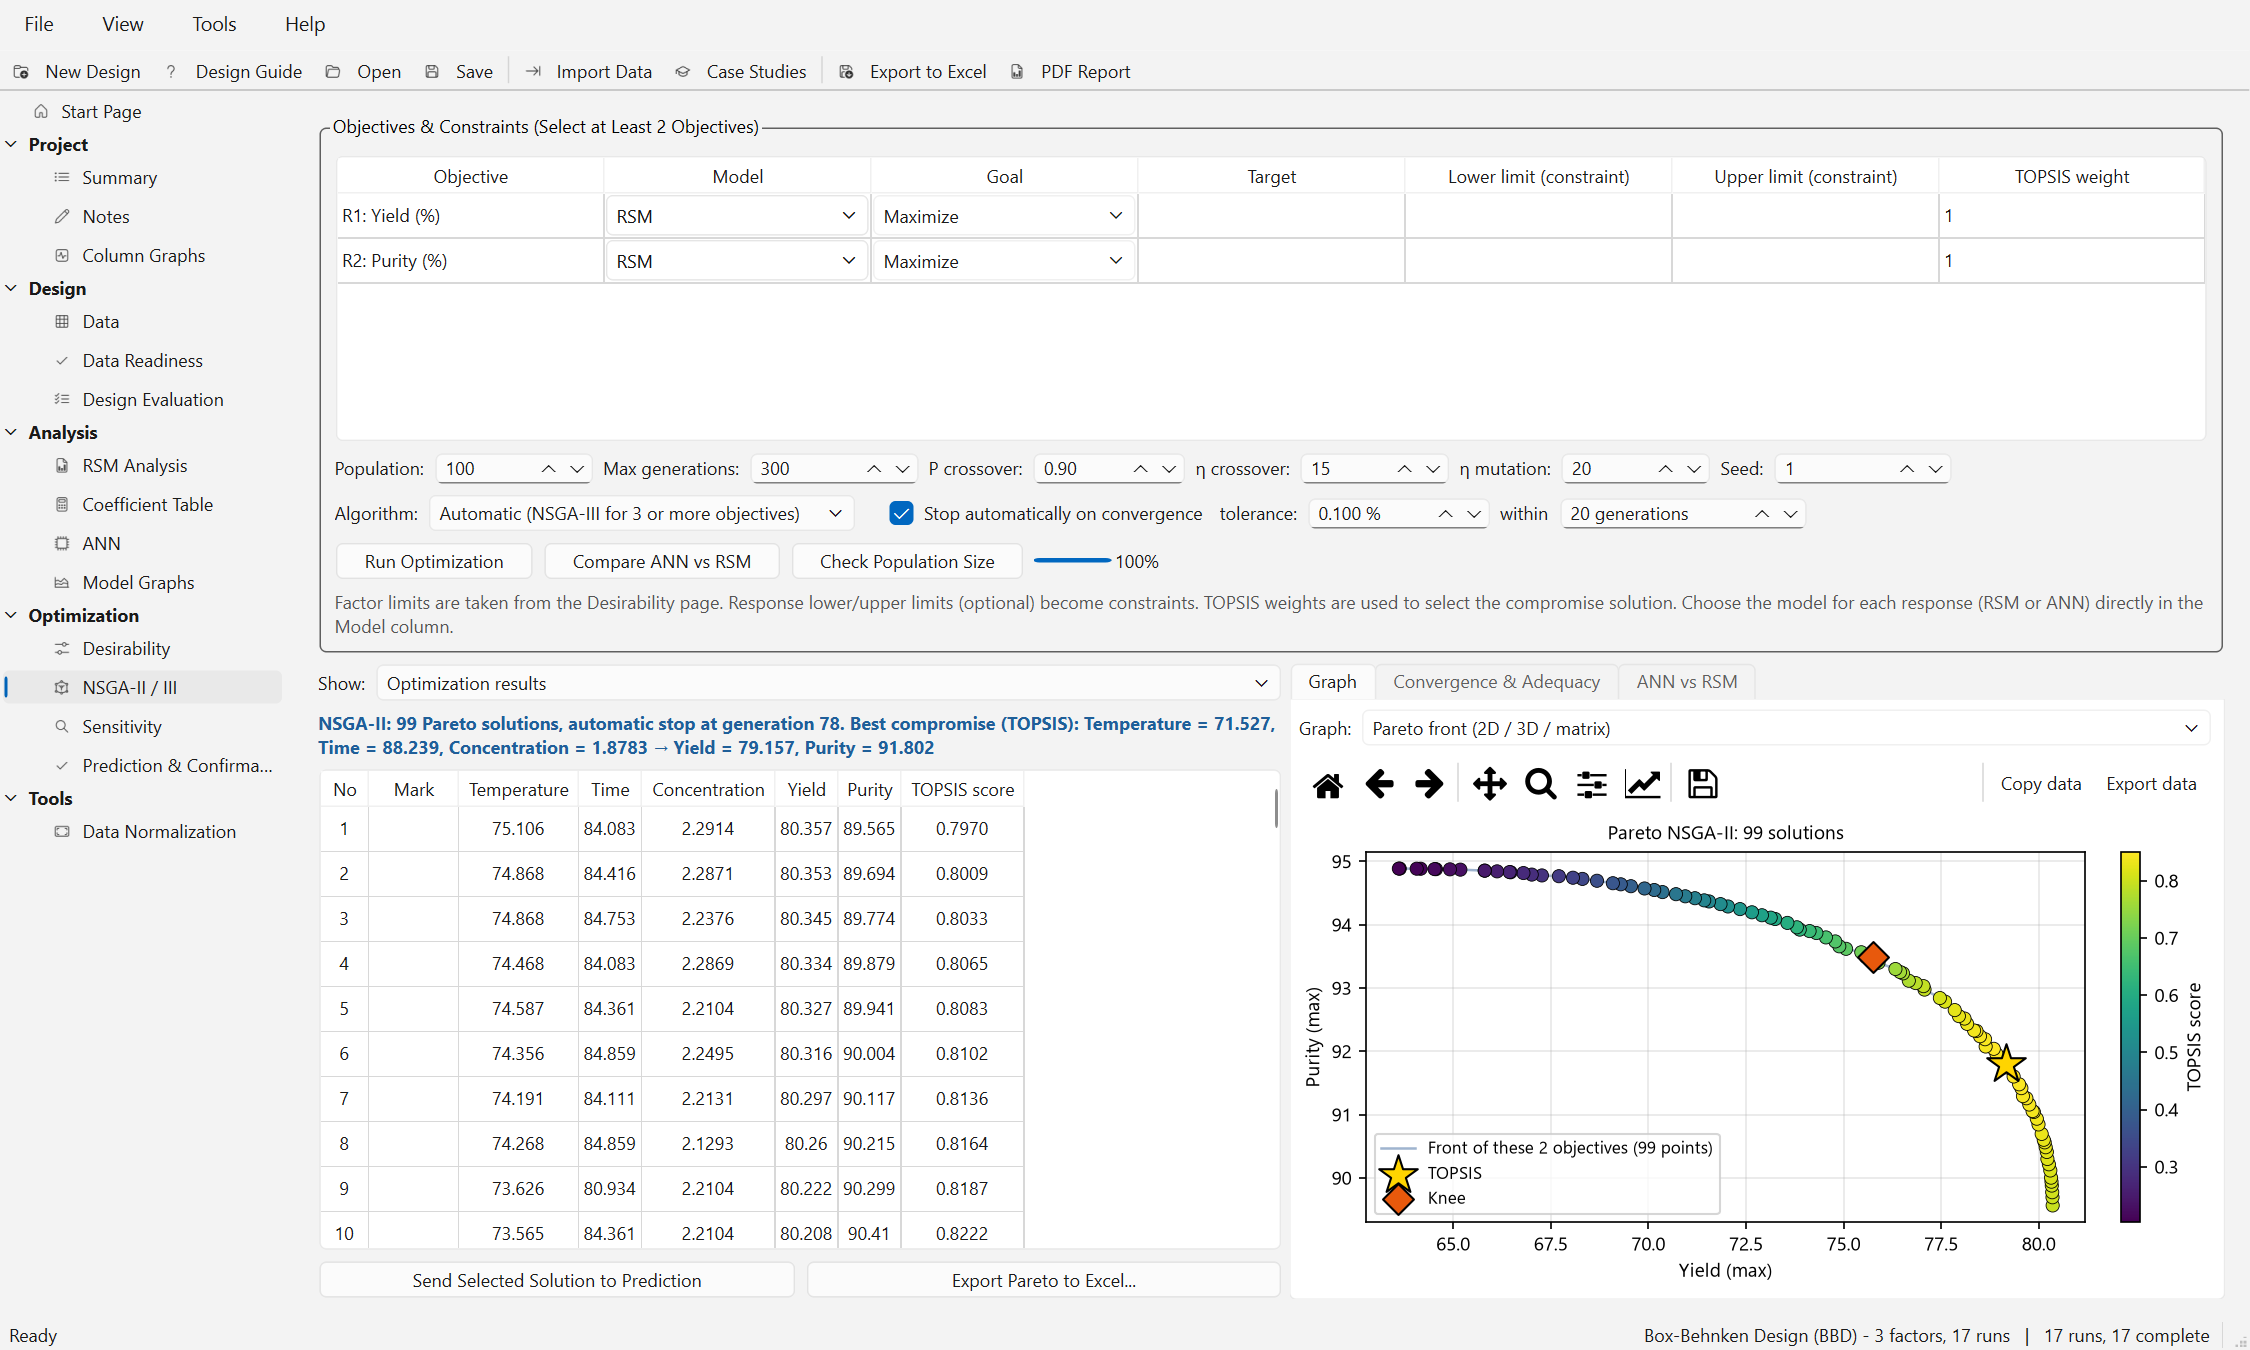
\includegraphics[width=\linewidth]{nsga_front.png}
\caption{NSGA-II front of the BBD case (Yield and Purity maximized, RSM models). Points are colored by TOPSIS score;
star = TOPSIS choice, diamond = knee point.}
\label{fig:ch08-front}
\end{figure}

The front (Figure~\ref{fig:ch08-front}) runs from Purity 94.89 at Yield 63.6 to Purity 89.57 at Yield 80.36: a
clear conflict between the two responses. Along most of the front, Purity falls slowly while Yield rises; above a
Yield of about 78 every further unit of Yield costs much more Purity. The knee lies at the start of this steep part,
and the TOPSIS choice lies inside it because TOPSIS with equal weights values the large Yield range.

\begin{figure}[htbp]
\centering
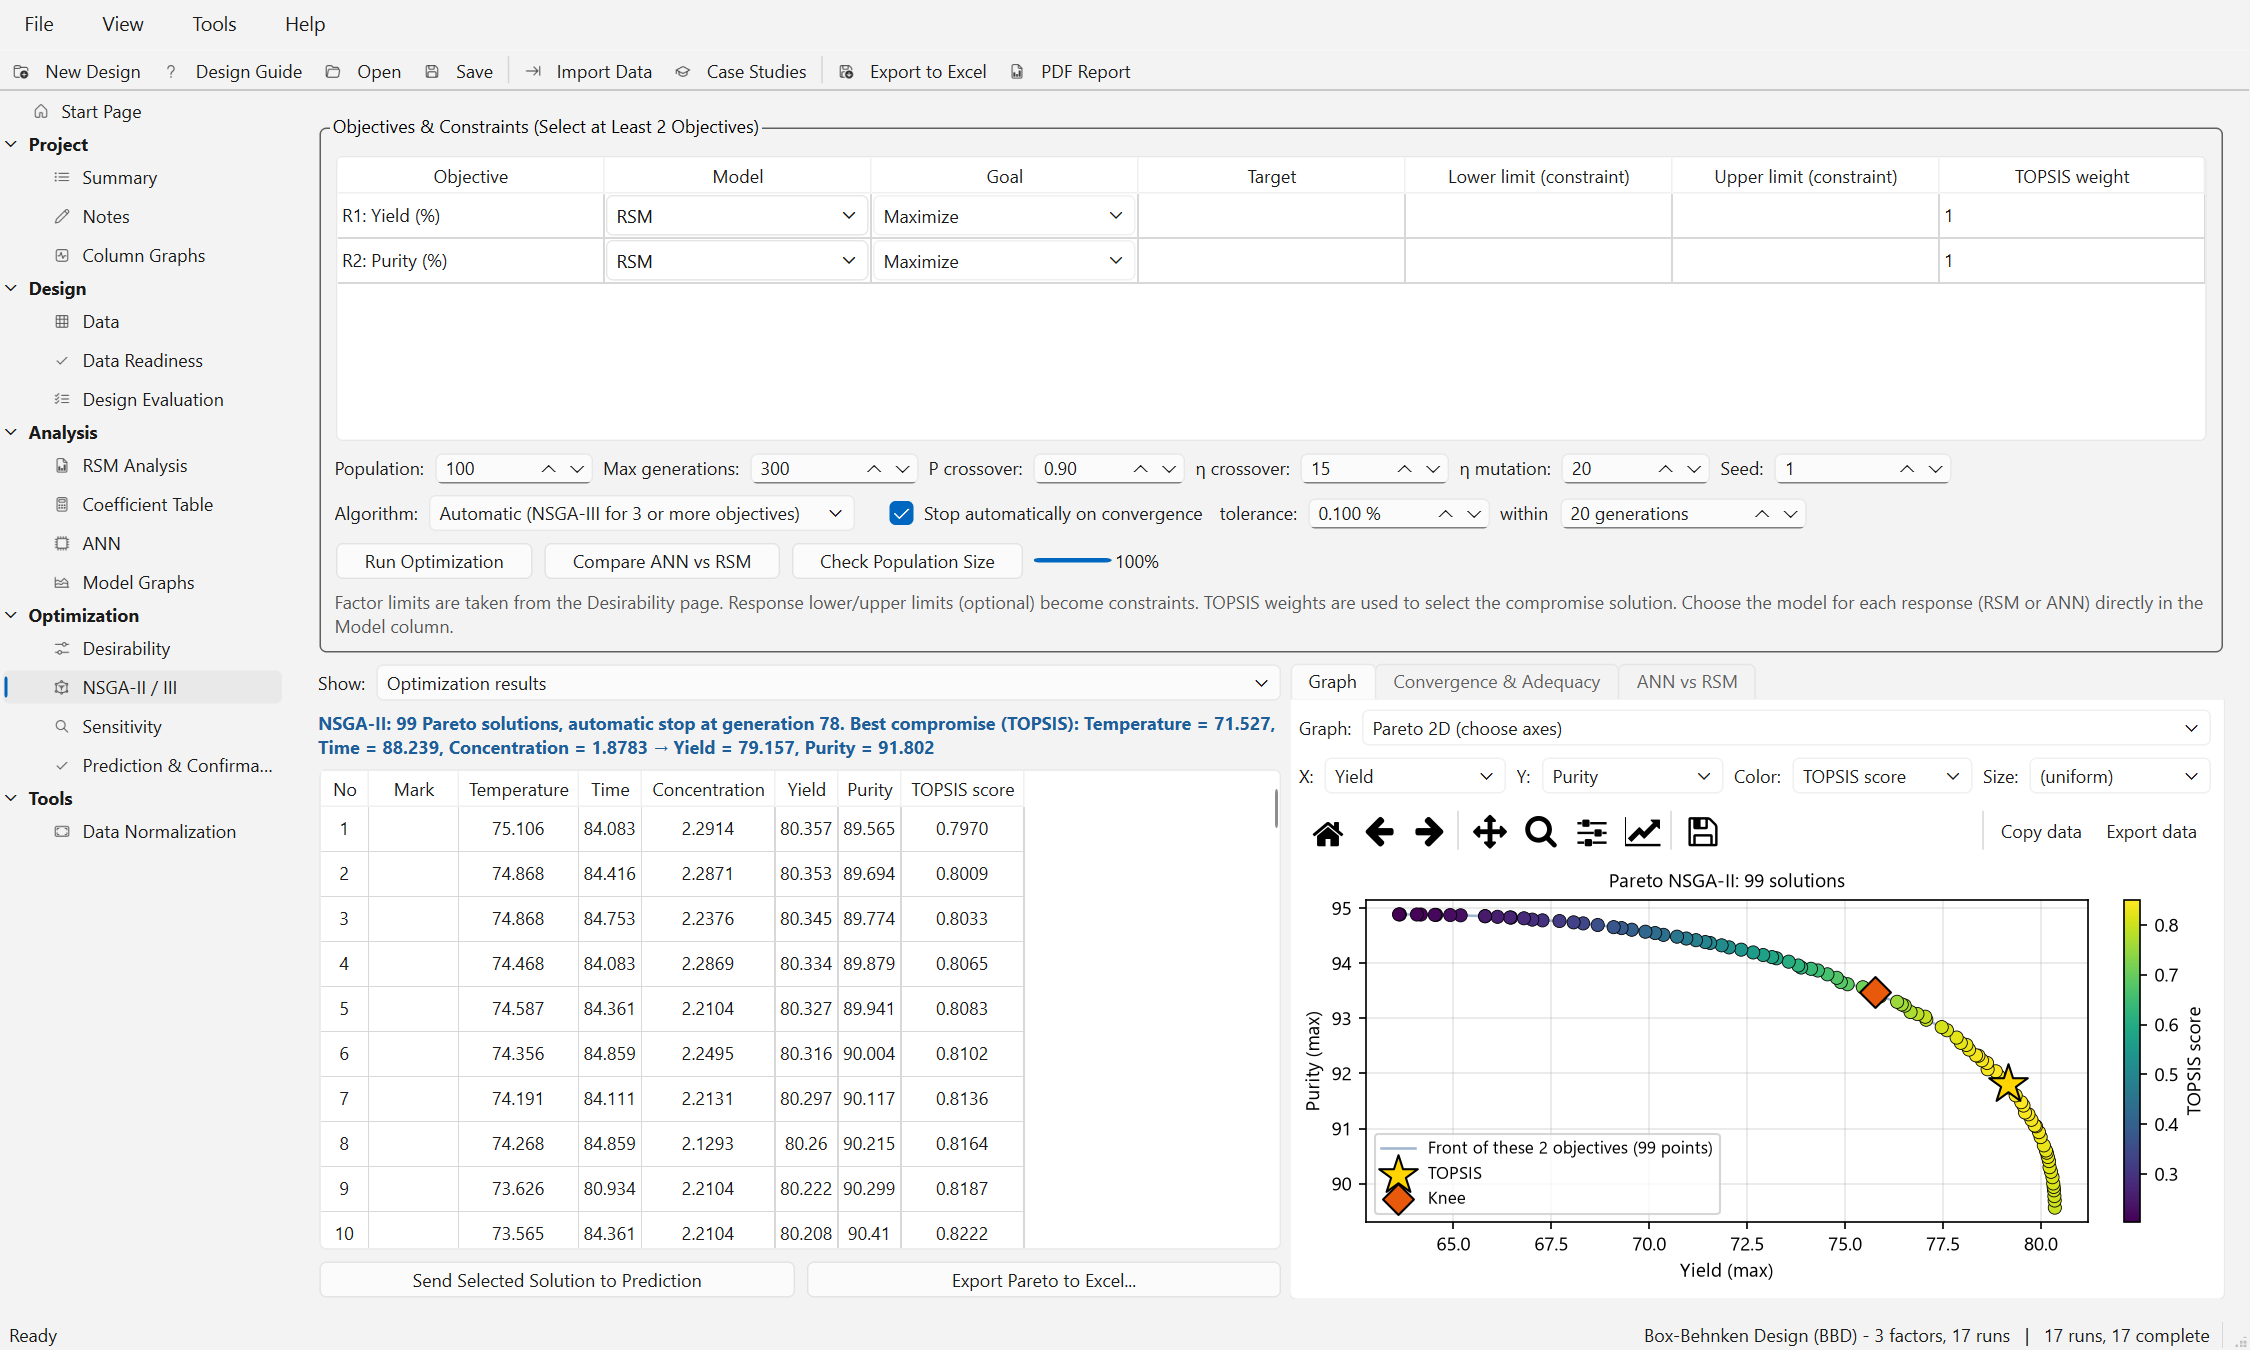
\includegraphics[width=\linewidth]{nsga_front2d.png}
\caption{\ui{Pareto 2D (choose axes)} with the \ui{X:}, \ui{Y:}, \ui{Color:} and \ui{Size:} selectors. With two
objectives it shows the same front as Figure~\ref{fig:ch08-front}.}
\label{fig:ch08-front2d}
\end{figure}

\begin{figure}[htbp]
\centering
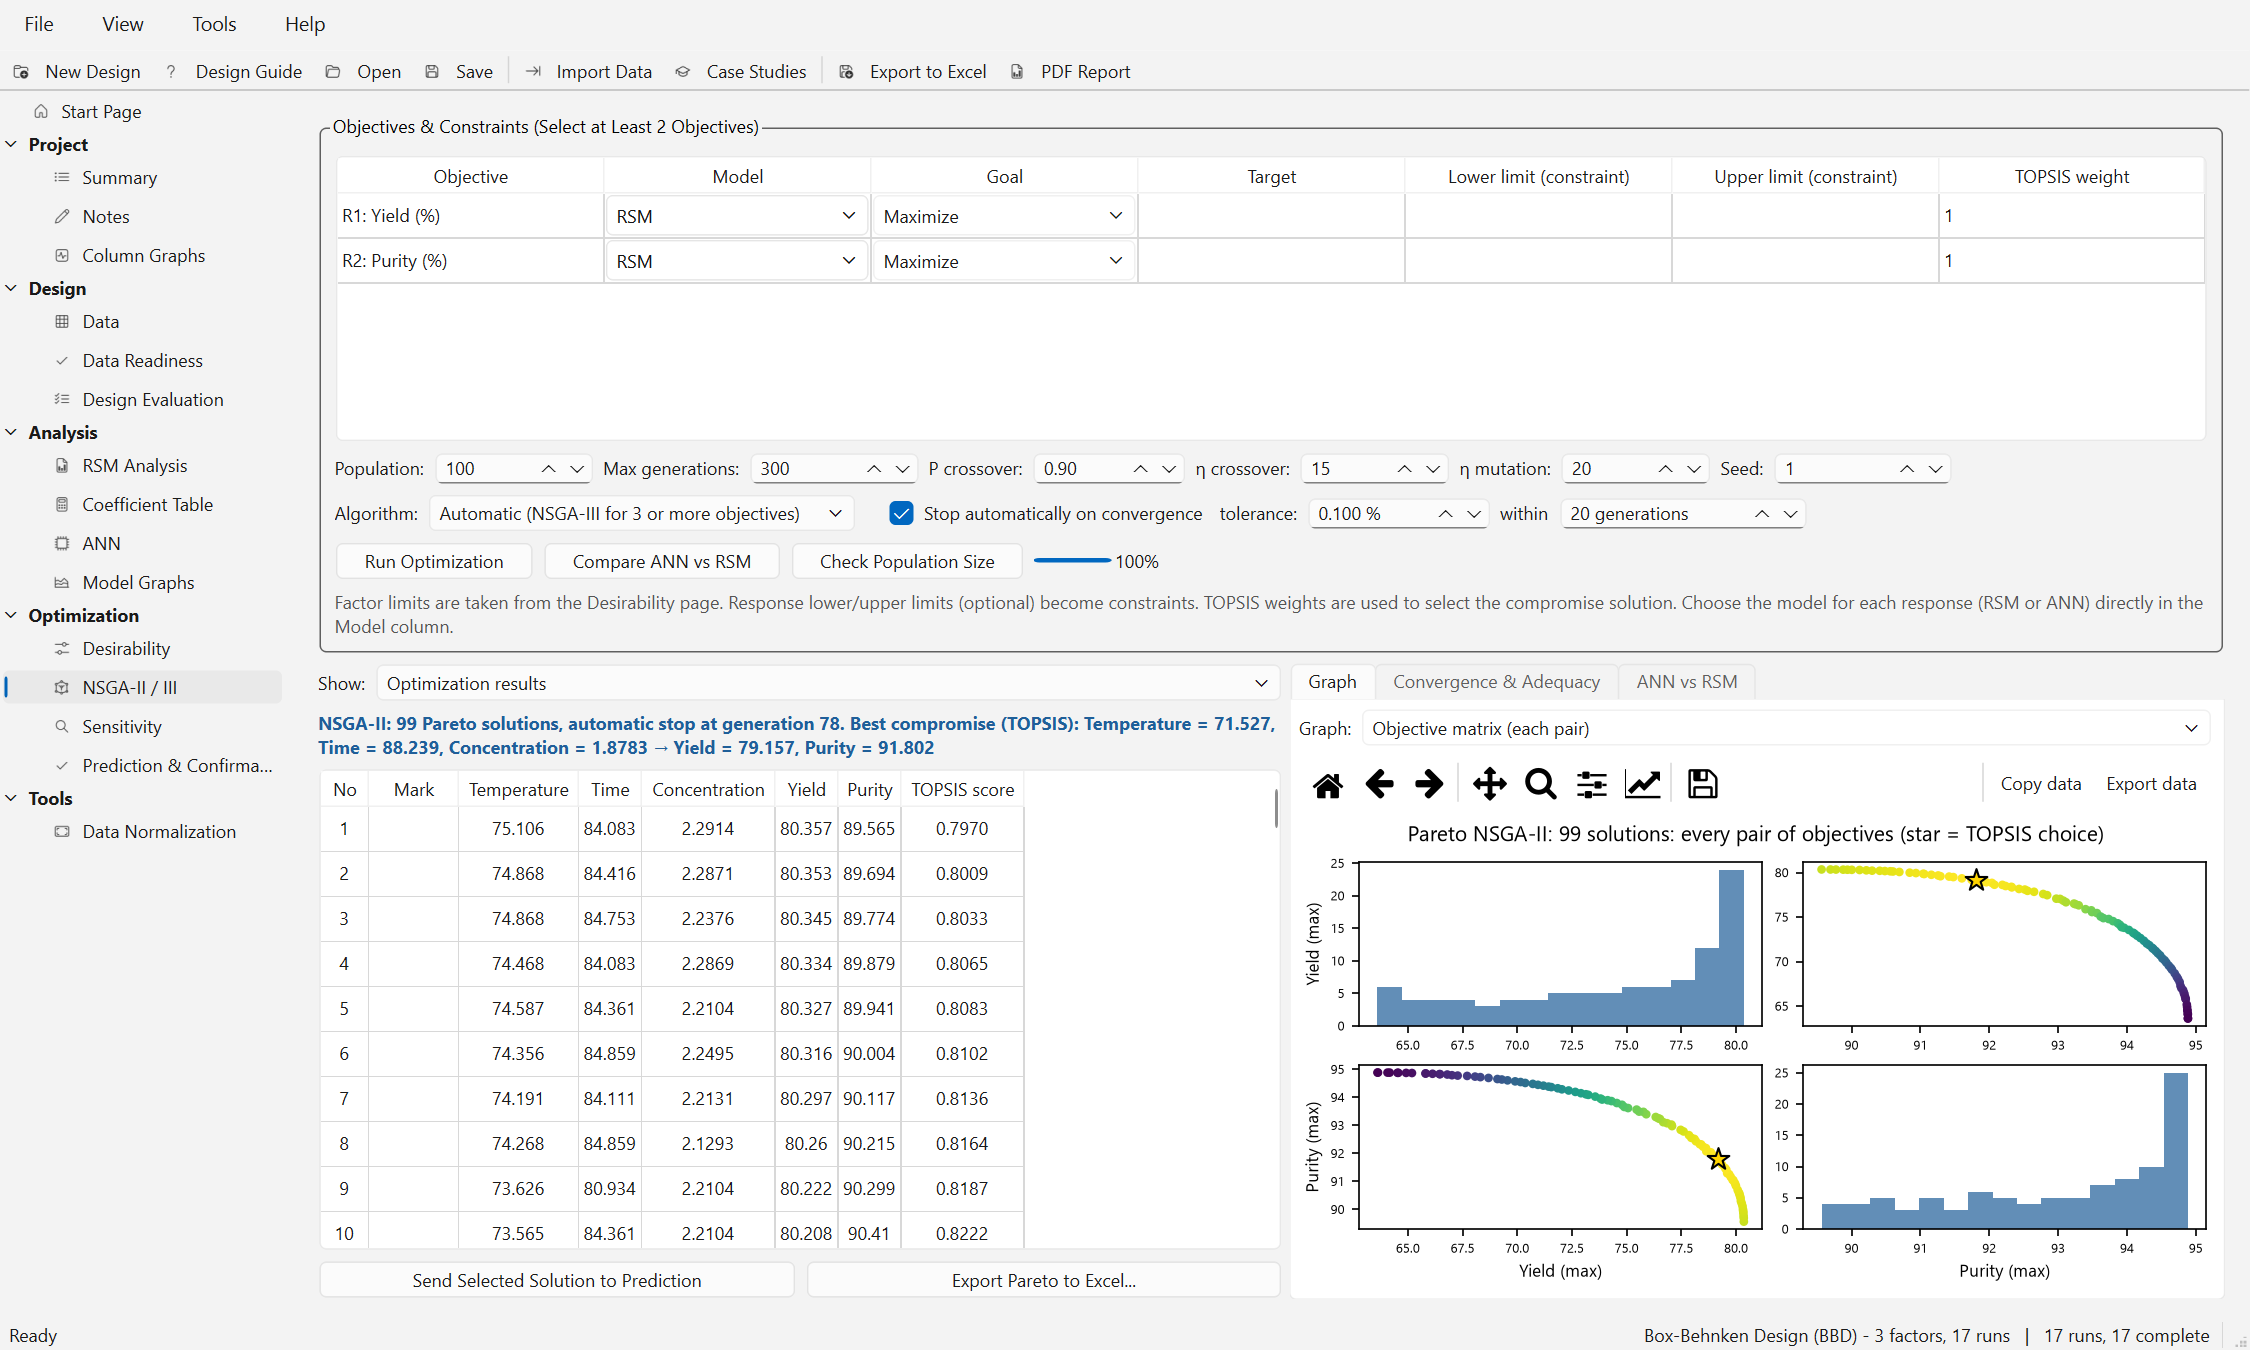
\includegraphics[width=\linewidth]{nsga_matrix.png}
\caption{\ui{Objective matrix (each pair)}: pairwise scatter plots and histograms of the objectives (most useful
for three or more objectives).}
\label{fig:ch08-matrix}
\end{figure}

\begin{figure}[htbp]
\centering
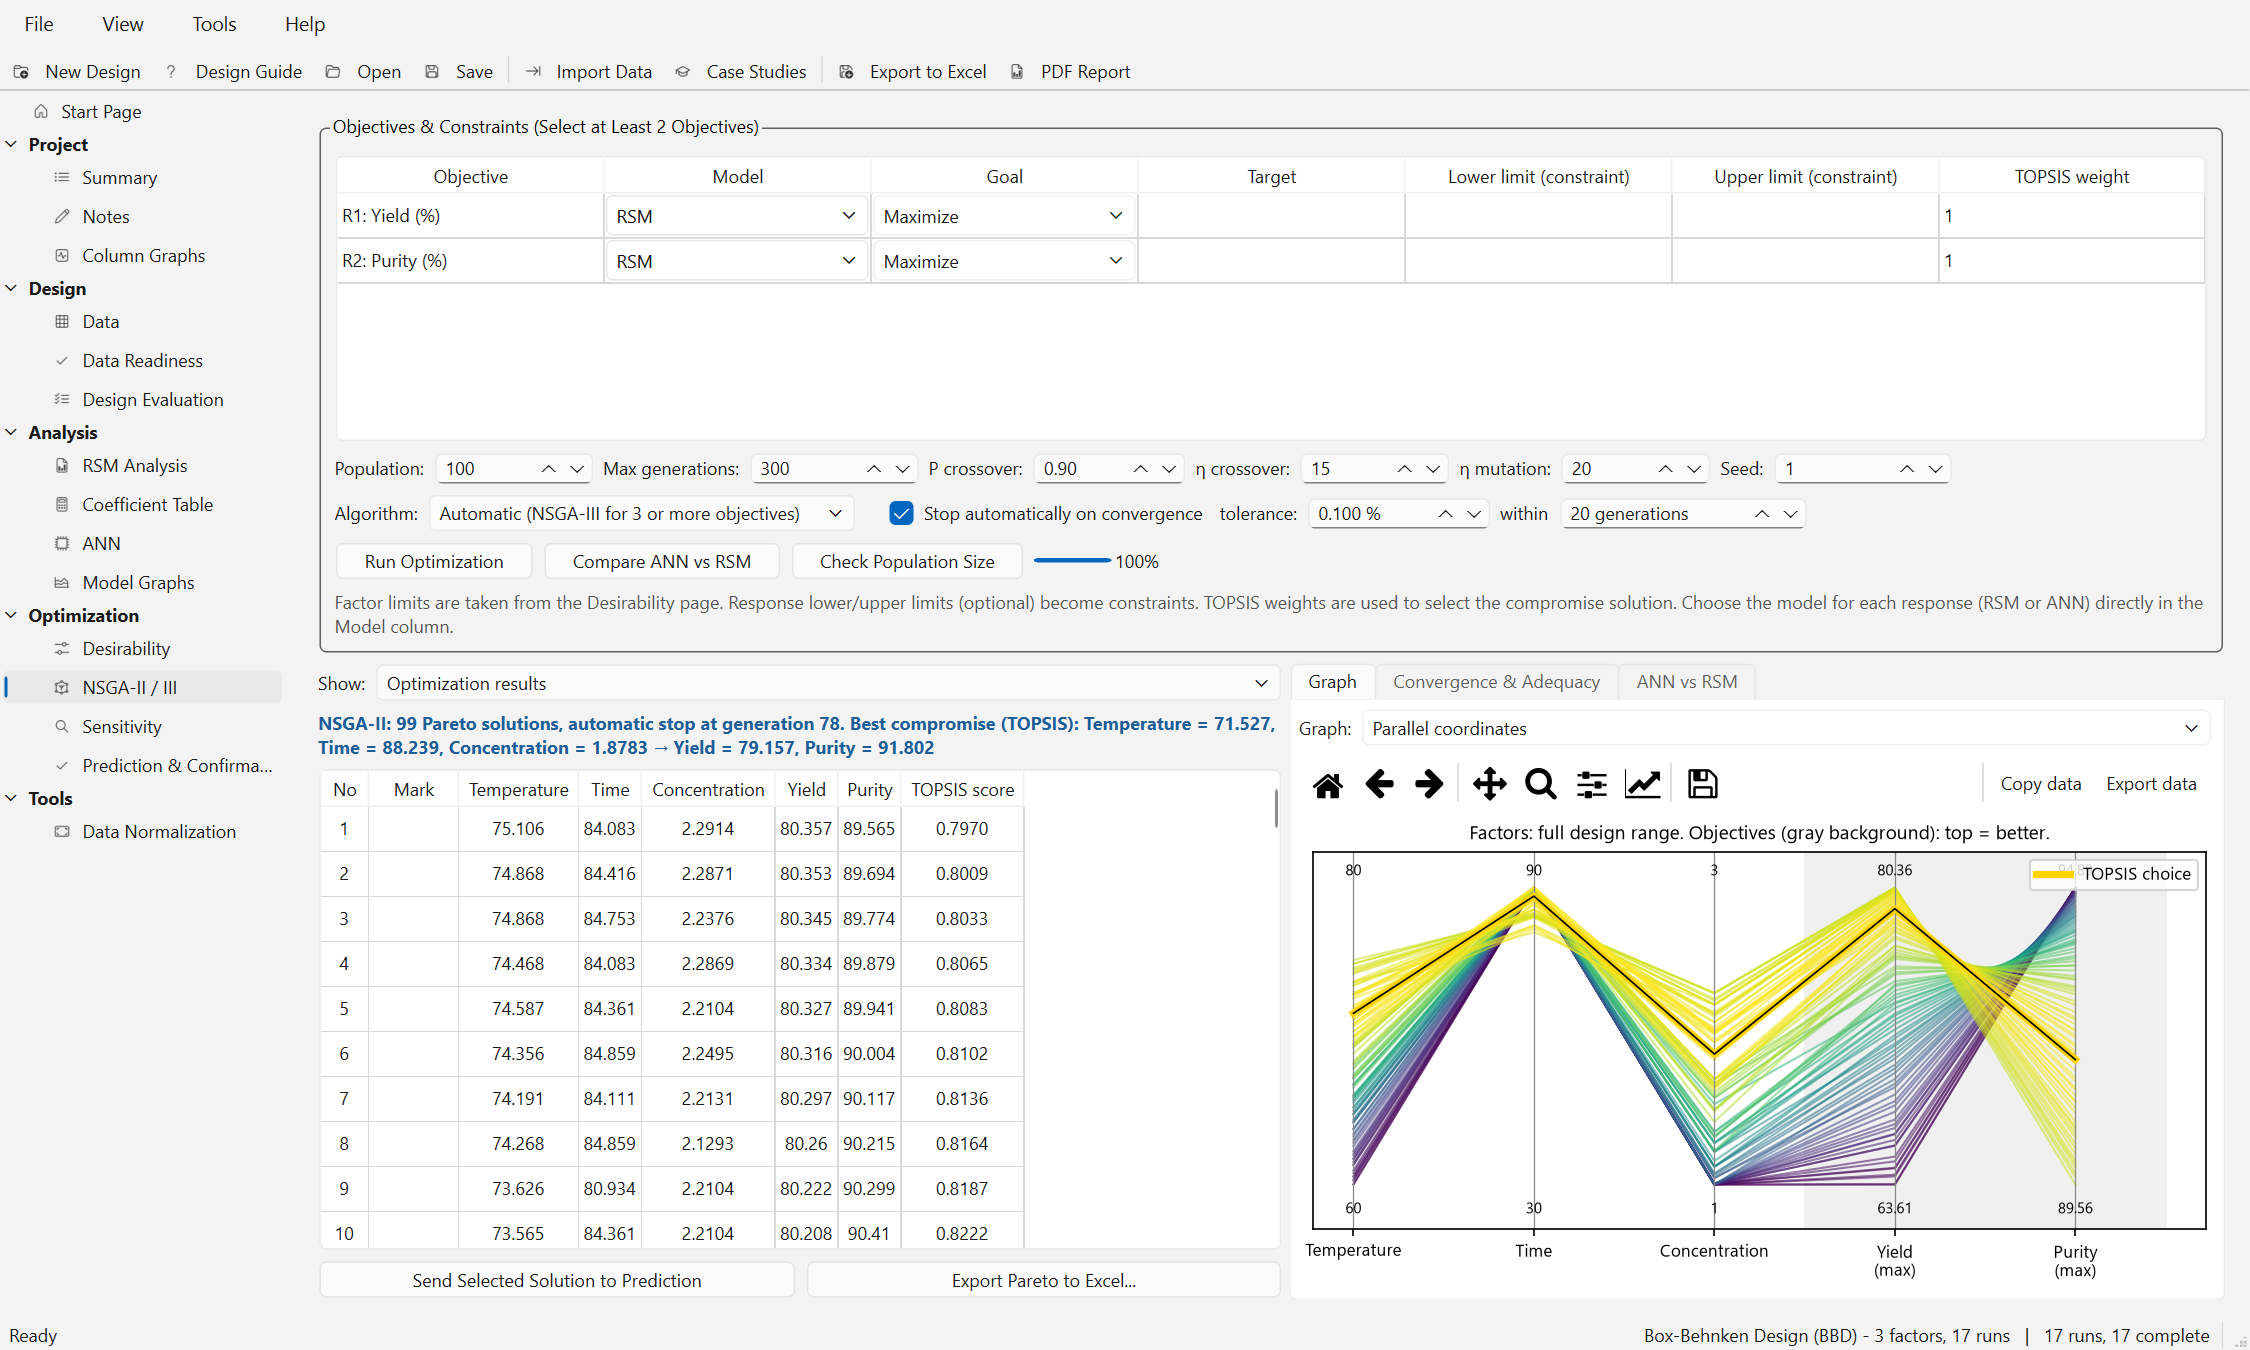
\includegraphics[width=\linewidth]{nsga_parallel.png}
\caption{\ui{Parallel coordinates}: each Pareto solution is a line across the factors (full design range) and the
objectives (grey, top = better); the TOPSIS solution is highlighted.}
\label{fig:ch08-parallel}
\end{figure}

The parallel coordinates (Figure~\ref{fig:ch08-parallel}) show how the front is built: Time stays at or near its upper
limit of 90~min for most solutions (it drops to about 81~min only at the high-Yield end), while Temperature (about 60 to 75~°C) and Concentration (1 to 2.3~\%)
increase together from the high-Purity end to the high-Yield end. Chapter~\ref{chap:9} quantifies this with Spearman
correlations along the front.

\begin{figure}[htbp]
\centering
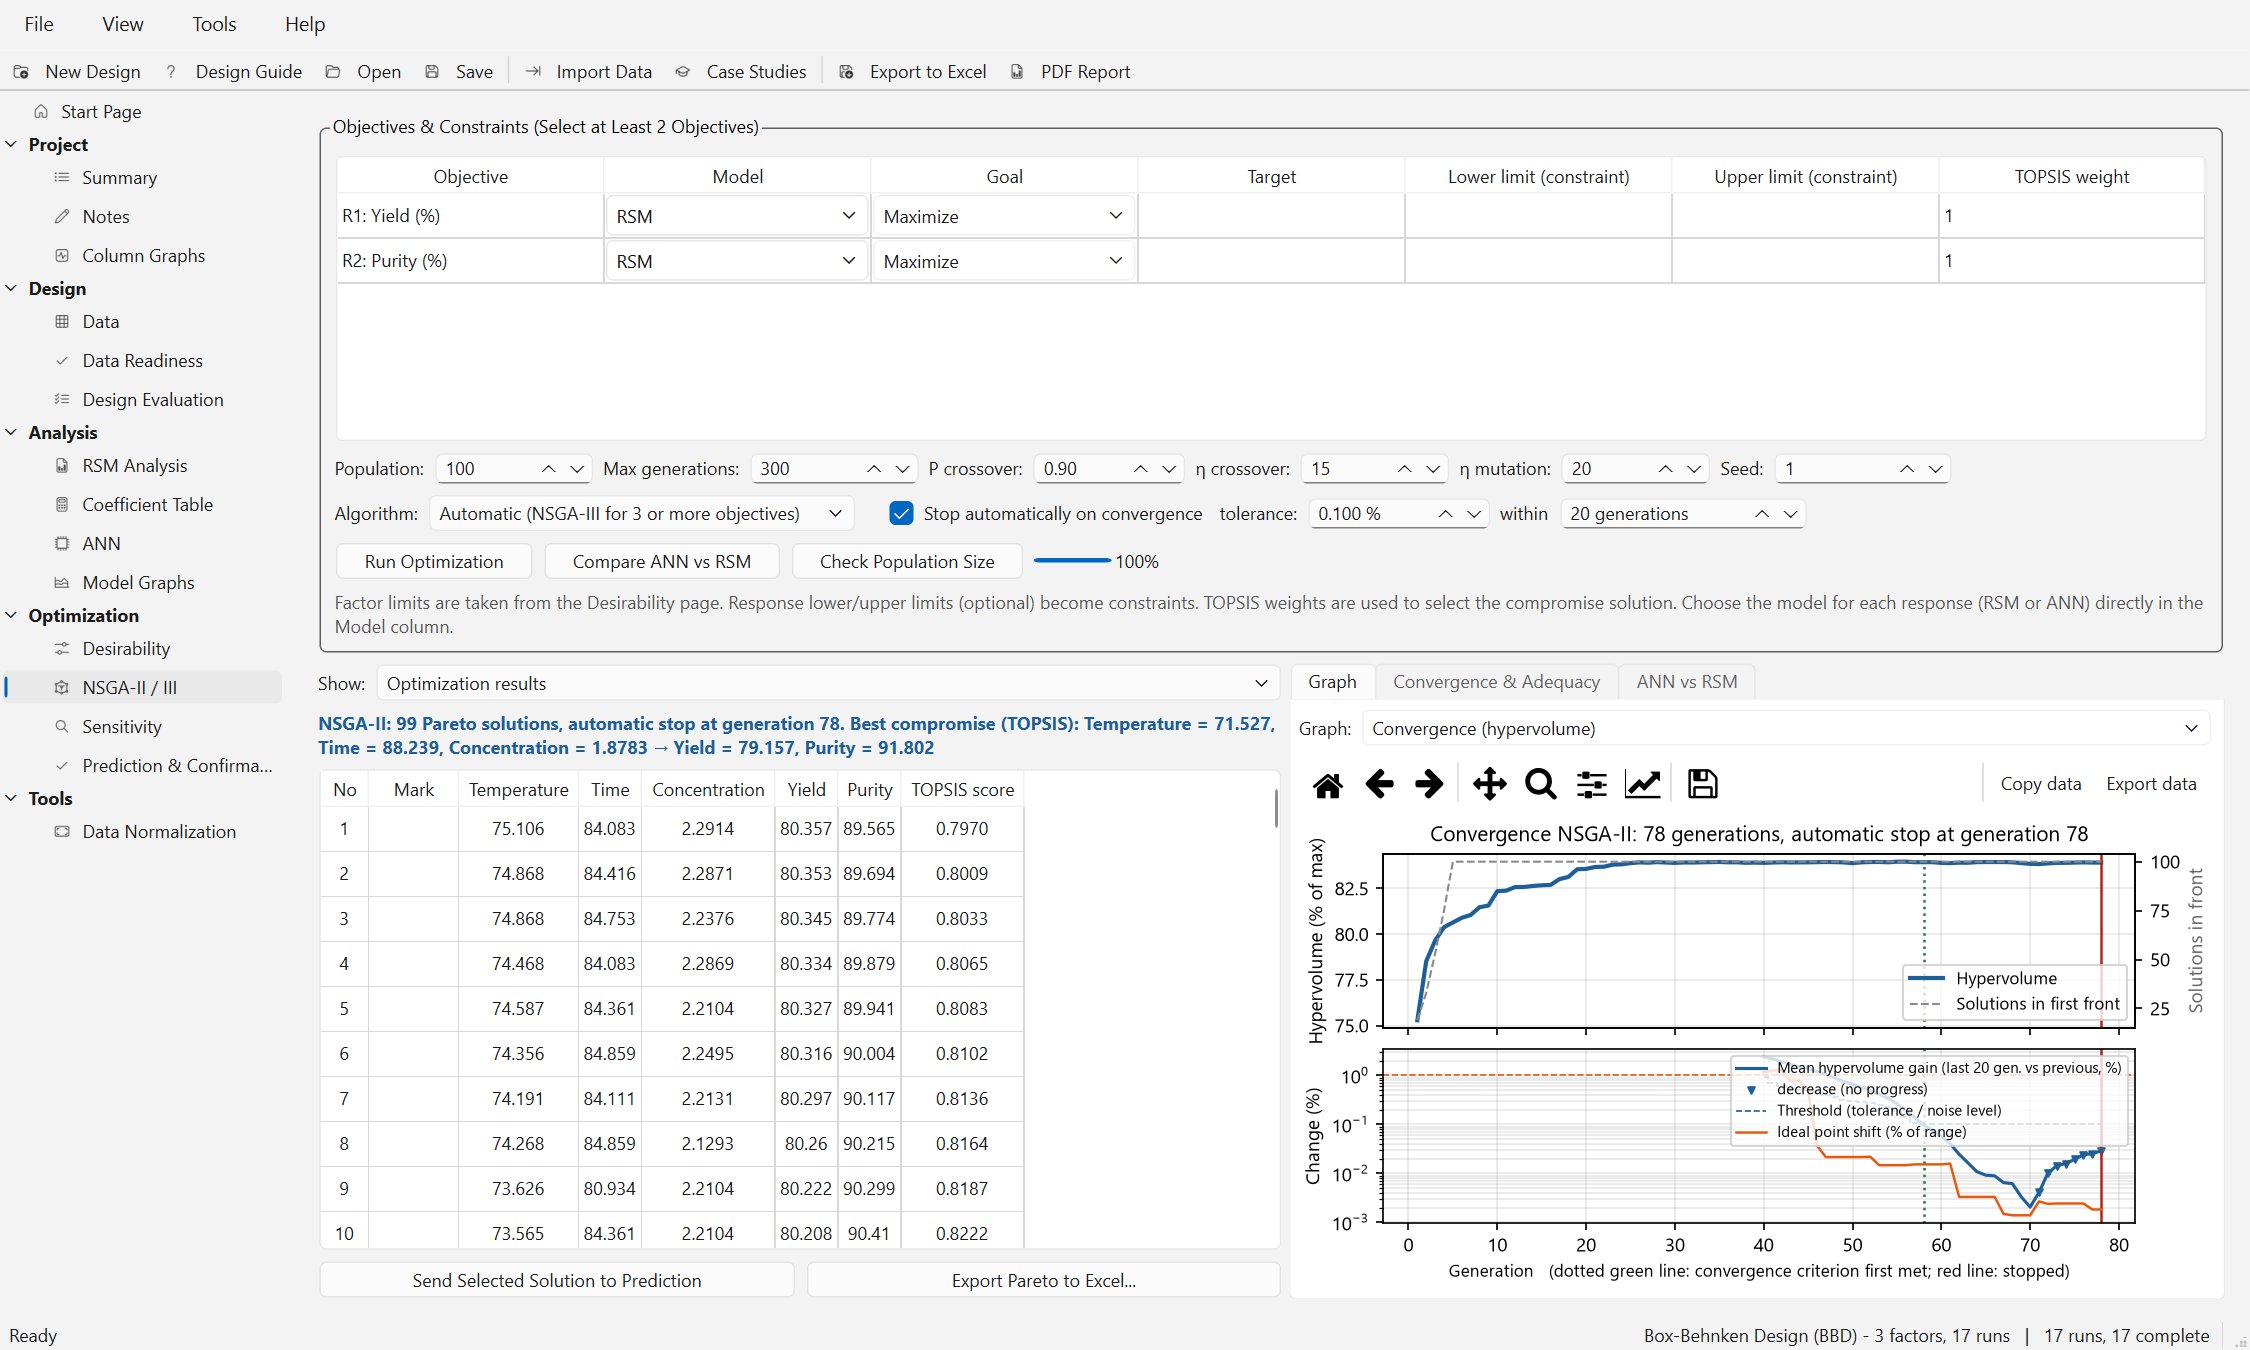
\includegraphics[width=\linewidth]{nsga_convergence.png}
\caption{\ui{Convergence (hypervolume)} of the BBD run: the hypervolume flattens near 84~\% of the maximum; the
criterion is first met at generation 58 (green dotted line) and the run stops at generation 78 (red line).}
\label{fig:ch08-convergence}
\end{figure}

Check~C (Figure~\ref{fig:ch08-convergence}): the hypervolume rises quickly in the first 20 generations and flattens
at 83.9~\% of $1.1^2$. From generation 40 on the gain is compared with the tolerance; the criterion
\eqref{eq:ch08-crit} is first met at generation 58 and holds for the next 20 generations, so the run stops at
generation 78. The report states: \ui{Enough generations: the mean hypervolume of the last 20 generations changed
by only -0.029\% compared with the previous 20 generations (limit 0.10\%) and the ideal point shifted 0.00\% (limit
1\%).} and \ui{All 100 individuals are on the first front (normal for 2 objectives).}

\begin{figure}[htbp]
\centering
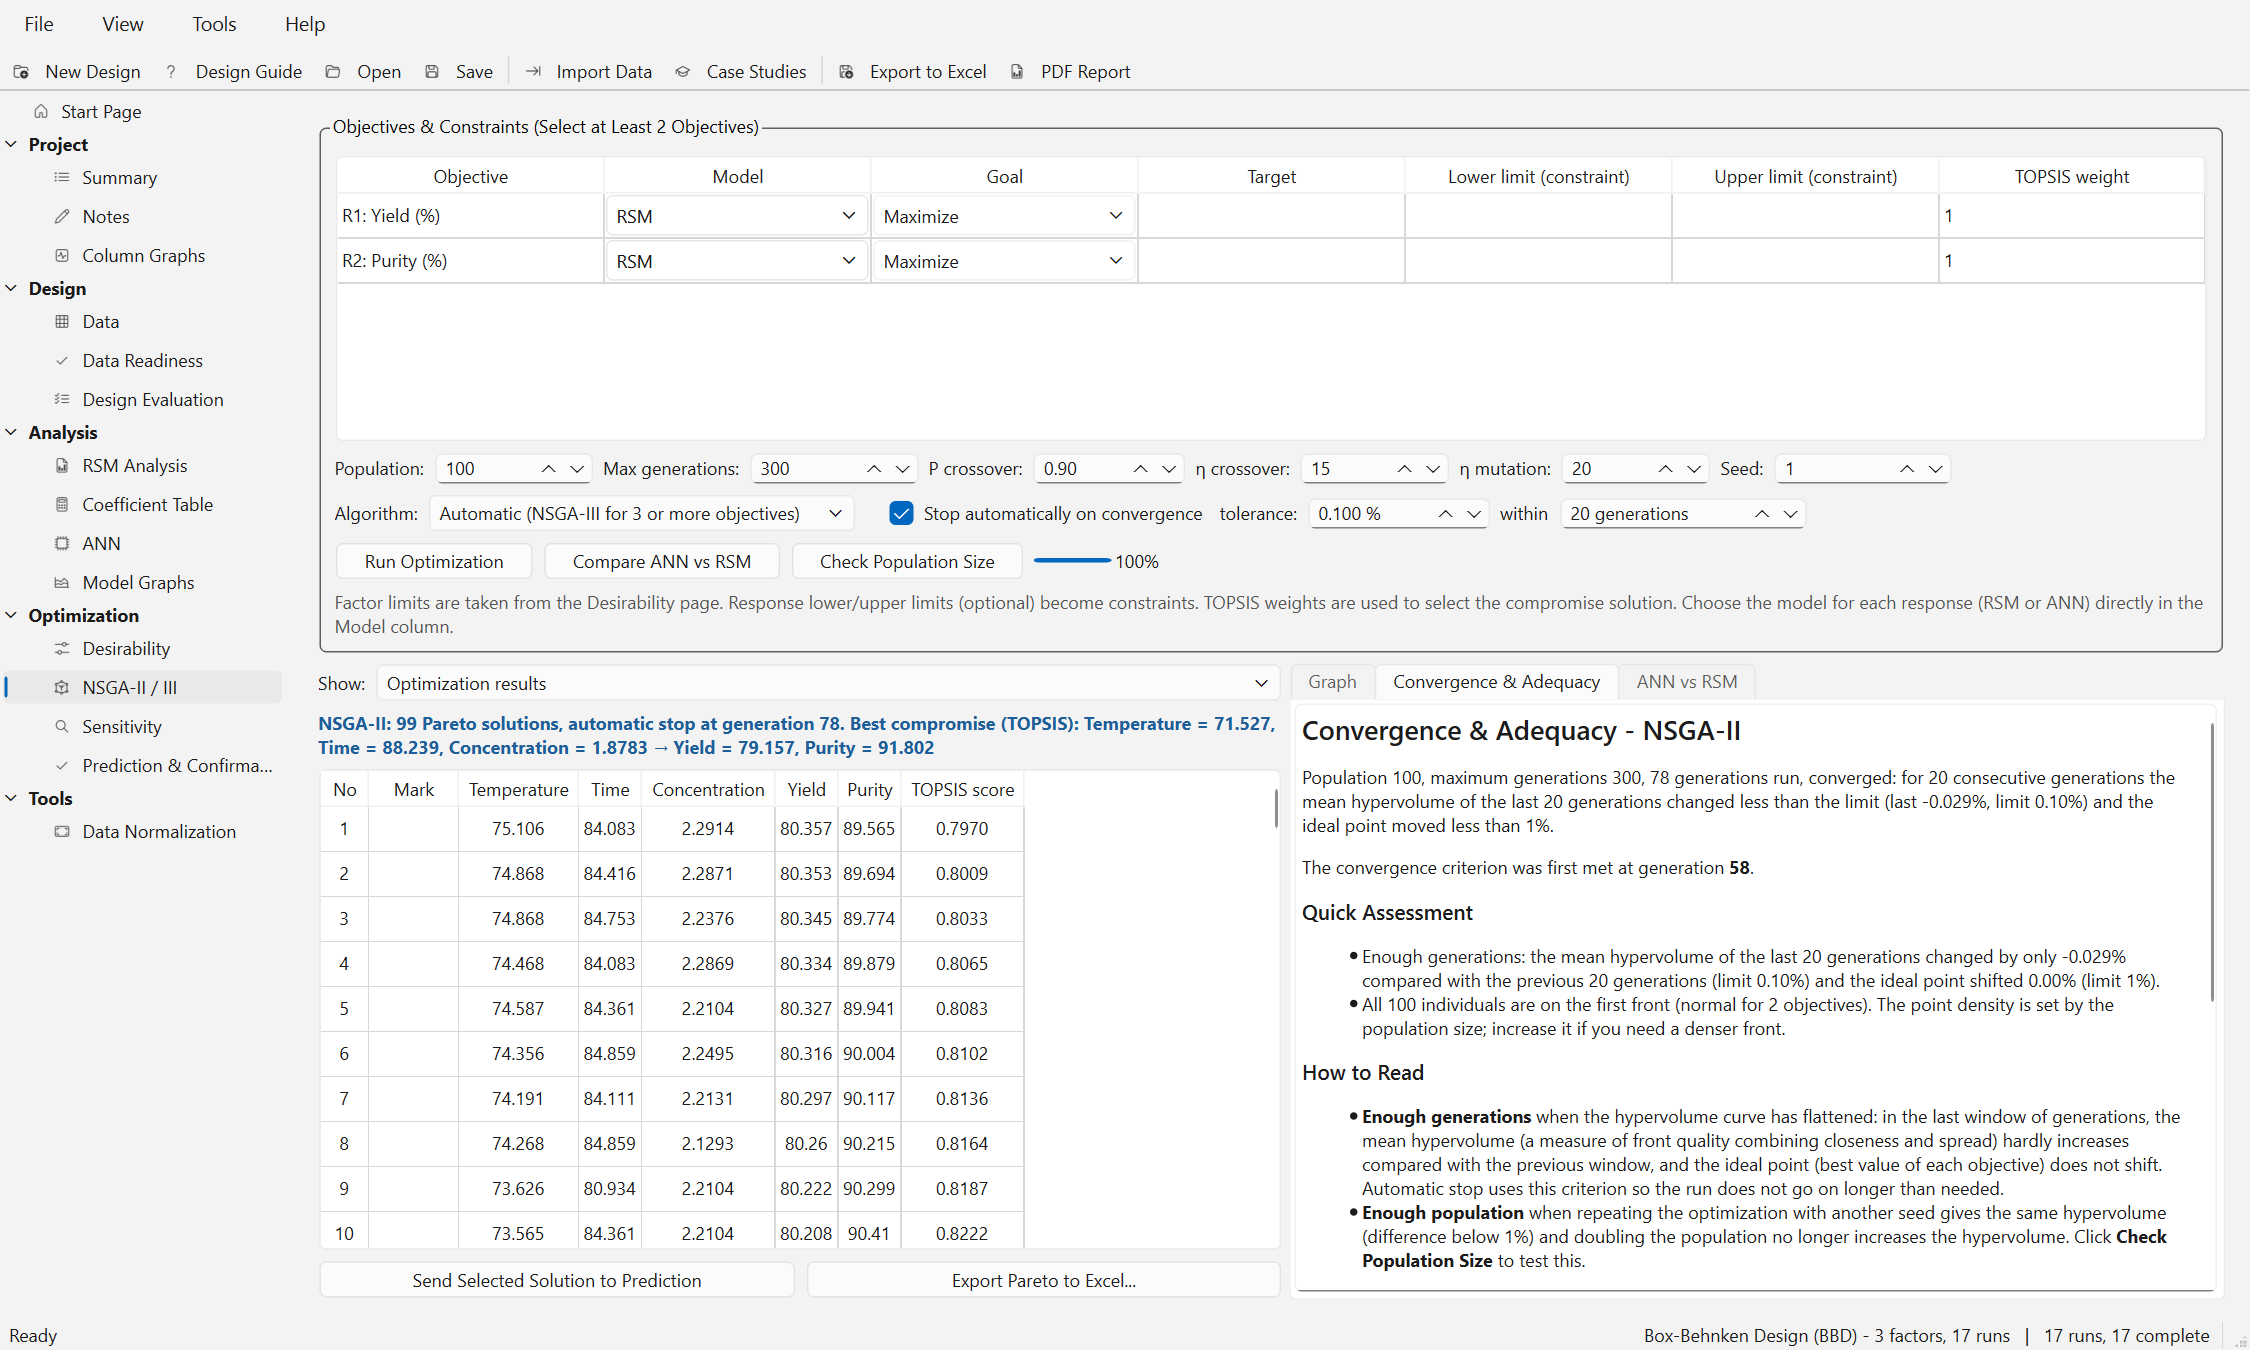
\includegraphics[width=\linewidth]{nsga_population_check.png}
\caption{\ui{Convergence \& Adequacy} tab after \ui{Check Population Size}. The upper part shows the quick
assessment; the table \ui{Adequacy Check Results} follows further down in the report.}
\label{fig:ch08-popcheck}
\end{figure}

\ui{Check Population Size} (Figure~\ref{fig:ch08-popcheck}) gives the results of
Table~\ref{tab:ch08-popcheck}. Another seed changes the hypervolume by at most 0.02~\% and a doubled population adds
0.35~\%, both below 1~\%: \ui{Population: sufficient. Another seed changes the hypervolume by only 0.02\% and a 2x
population adds only 0.35\%.} The TOPSIS choice moves by at most 5.5~\% of a factor range, well below the 15~\%
note. Check~C is therefore passed: the front of this run can be reported.

\begin{table}[htbp]
\centering
\small
\caption{\ui{Adequacy Check Results} for the BBD run (NSGA-II, population 100, seed 1).}
\label{tab:ch08-popcheck}
\begin{tabular}{@{}lrrlrrrr@{}}
\toprule
Run & Pop. & Seed & Generations & Solutions & HV & Diff. & TOPSIS shift (\%) \\
\midrule
Current result & 100 & 1 & 78 (converged) & 99 & 83.93\% & +0.00\% & 0.0 \\
Different seed & 100 & 102 & 70 (converged) & 100 & 83.93\% & +0.01\% & 5.5 \\
Different seed 2 & 100 & 203 & 81 (converged) & 100 & 83.94\% & +0.02\% & 2.2 \\
Population 2x & 200 & 1 & 67 (converged) & 195 & 84.22\% & +0.35\% & 2.9 \\
\bottomrule
\end{tabular}
\end{table}

\textbf{When check C fails.} If the quick assessment says \ui{Not enough generations yet}, increase \ui{Max
generations} (the automatic stop still ends the run when it converges). If the population check is not passed,
double the population and check again. With three or more objectives a saturated first front (all $N$ members
non-dominated) is a hint that the population is too small to describe the front. In the three-objective POE example
above the noise level raised the threshold \eqref{eq:ch08-tau} from 0.10~\% to 0.25~\%, and the quick assessment
recommended \ui{try 2x the population and compare}.

% ======================================================================================================
\section{Check D: ANN versus RSM fronts}
\label{sec:ch08-checkD}

\subsection{Purpose}
An optimum found on a model is only as good as the model. When both an RSM and an ANN model are available, check~D
asks whether the optimization result depends on the choice of model. If the two models predict similar values on
the Pareto solutions and lead to similar compromise settings, the result is robust. If they disagree, the
disagreement marks the region where the data do not determine the response well enough, the same idea used to
locate uncertain regions with disagreeing networks \citep{krogh1995}. Confirmation runs are then needed at both
candidate settings.

\subsection{How to use}
\begin{enumerate}
  \item Train an ANN for the objective responses on the ANN page, preferably with \ui{Optimize All Responses (One
        Click)} so that each network is selected by cross-validation (check~A, Chapter~\ref{chap:7}). Without any ANN the button
        answers \ui{There is no ANN model for the objective responses yet. Train an ANN first on the ANN page
        (Optimize All Responses button).}
  \item Set the objectives as for a normal run and click \ui{Compare ANN vs RSM}. The progress text shows
        \ui{[1/2] RSM: \dots} and \ui{[2/2] ANN: \dots}.
  \item Read the \ui{ANN vs RSM} tab and the three comparison graphs. With \ui{Show:} you can inspect each front in
        the solutions table.
\end{enumerate}

\subsection{Theory as implemented}
\begin{enumerate}
  \item The optimization is run twice with identical settings: once with RSM for every objective and once with ANN
        for every objective. A response without an ANN keeps its RSM model on the ANN front (warning \ui{No ANN yet
        for \dots; on the ANN front these responses still use RSM.}).
  \item \textbf{Cross-prediction.} The solutions of each front are predicted with the other model, giving
        $y^\text{self}$ and $y^\text{other}$ for every solution of both fronts.
  \item \textbf{Hypervolume.} The four objective sets (RSM front by RSM, RSM front by ANN, ANN front by ANN, ANN
        front by RSM) are normalized jointly, and $HV_{(\text{front, assessor})}$ is computed as in check~C (in \%
        of $1.1^m$).
  \item \textbf{Prediction difference.} For each objective $o$, over the solutions of both fronts,
        \begin{equation}
        \Delta_o^\text{mean}=\frac{100}{R_o}\operatorname{mean}\bigl|y^\text{self}-y^\text{other}\bigr|,\qquad
        \Delta_o^\text{max}=\frac{100}{R_o}\max\bigl|y^\text{self}-y^\text{other}\bigr|,
        \label{eq:ch08-delta}
        \end{equation}
        where $R_o$ is the range (maximum minus minimum) of the response data; for a POE objective it is the range
        of all predicted POE values. The decisive value is the worst objective,
        $\Delta=\max_o\Delta_o^\text{mean}$.
  \item \textbf{Distance between the compromise choices.} With $\mathbf x^\text{RSM}$ and $\mathbf x^\text{ANN}$ the
        TOPSIS solutions of the two fronts (coded units) and $[l_j,u_j]$ the coded design range,
        \begin{equation}
        dx=100\,\max_j\frac{|x^\text{RSM}_j-x^\text{ANN}_j|}{u_j-l_j}.
        \label{eq:ch08-dx}
        \end{equation}
  \item \textbf{Model quality} per objective: RSM predicted $R^2$, ANN test $R^2$ of the final model's single
        split, and ANN cross-validation $Q^2$ from the architecture search (if one was run).
\end{enumerate}

\subsection{Conclusion rules and messages}
\begin{table}[htbp]
\centering
\small
\caption{Verdict of check~D ($\Delta$ in \% of the response range, $dx$ in \% of the factor range).}
\label{tab:ch08-checkD}
\begin{tabularx}{\linewidth}{@{}>{\raggedright\arraybackslash}p{2.4cm} >{\raggedright\arraybackslash}p{3.2cm} >{\raggedright\arraybackslash}X@{}}
\toprule
Verdict & Condition & Message (beginning) and action \\
\midrule
Agree (green) & $\Delta<5$ and $dx<15$ & \ui{Both models agree: predictions on the front differ by only \dots\ The
optimization result does not depend on the choice of model.} \\
Partial (amber) & $\Delta<10$, not ``agree'' & \ui{The models agree only partly.} followed by the criterion that
failed: both (\ui{Make confirmation runs at both TOPSIS points.}), only $\Delta$ (\ui{Check the region where the
differences are largest before relying on the front there.}) or only $dx$ (\ui{The front is flat in that region:
several settings give similar results.}). \\
Differ (red) & $\Delta\ge10$ & \ui{The models differ considerably: \dots\ Do not rely on just one model: make
confirmation runs at both TOPSIS points.} The $dx$ part states whether it is within or above 15~\%. \\
\bottomrule
\end{tabularx}
\end{table}
The thresholds are 5~\% and 10~\% for $\Delta$ and 15~\% for $dx$. They are practical rules: a mean difference of
5~\% of the observed range is of the order of the prediction error of a good response surface model, and 15~\% of a
factor range is a distance at which two settings are clearly different experiments.

Further bullets of the conclusion:
\begin{itemize}
  \item \ui{According to each model, the ANN|RSM front promises a better trade-off (hypervolume $x$\% vs $y$\%).}
        compares $HV_{(\text{RSM,RSM})}$ with $HV_{(\text{ANN,ANN})}$.
  \item If a front loses more than 5 percentage points of hypervolume when assessed by the other model:
        \ui{The \dots\ front loses a lot of hypervolume when assessed by the other model. Its advantage may exist
        only in the \dots\ model (for example, ANN extrapolating or RSM being too simple).}
  \item \ui{Prediction accuracy on new data: RSM mean Pred R² \dots, ANN mean cross-validation Q² \dots. If the
        fronts differ, the model with higher accuracy is more trustworthy.} The ANN value is the mean
        cross-validation $Q^2$ of the architecture search when every objective has an ANN found by a search; it is
        more reliable than one train/test split of a small data set. Otherwise the bullet falls back to
        \ui{ANN mean test R² (single split)}, which for small data sets rests on very few runs; compare it with the
        \ui{Model Quality per Response} table.
\end{itemize}

\subsection{Report and plots}
The \ui{ANN vs RSM} tab contains the sections \ui{Pareto Front Comparison: ANN vs RSM}, \ui{Model Quality per
Response}, \ui{Front Size} (Pareto solutions, generations run, \ui{Hypervolume, assessed by own model} and
\ui{Hypervolume, assessed by other model}), \ui{Prediction Difference on Pareto Solutions} ($\Delta^\text{mean}$ and
$\Delta^\text{max}$), \ui{TOPSIS Compromise Solutions} (both choices with factor values and predictions of both
models, and $dx$) and \ui{Conclusion}. The graphs are:
\begin{description}[style=nextline]
  \item[\ui{ANN vs RSM: 2D front}] Both fronts on the chosen \ui{X:} and \ui{Y:} axes (RSM blue circles, ANN orange
        triangles). Filled stars are the TOPSIS choices; hollow stars are the same choices predicted by the other
        model, connected by dashed arrows. A long arrow means the other model disagrees about that setting.
  \item[\ui{ANN vs RSM: cross-prediction}] One panel per objective: RSM prediction against ANN prediction for the
        solutions of both fronts, with the 1:1 line; the panel title gives $\Delta^\text{mean}$.
  \item[\ui{ANN vs RSM: factors}] Parallel coordinates of the factor settings of both fronts over the full design
        range, with thick lines for the two TOPSIS choices.
\end{description}

\subsection{Example: BBD extraction}
\label{sec:ch08-checkD-example}
For the BBD case the ANNs were selected with \ui{Optimize All Responses (One Click)} (default search settings,
1 CPU core, seed 1): 3-4-1 for Yield (cross-validation $Q^2=0.624$) and 3-5-1 for Purity ($Q^2=0.774$), both
\ui{Good fit}. \ui{Compare ANN vs RSM} with the settings of Section~\ref{sec:ch08-nsga-example} gives
Figures~\ref{fig:ch08-cmp-front}--\ref{fig:ch08-cmp-report}.

\begin{figure}[htbp]
\centering
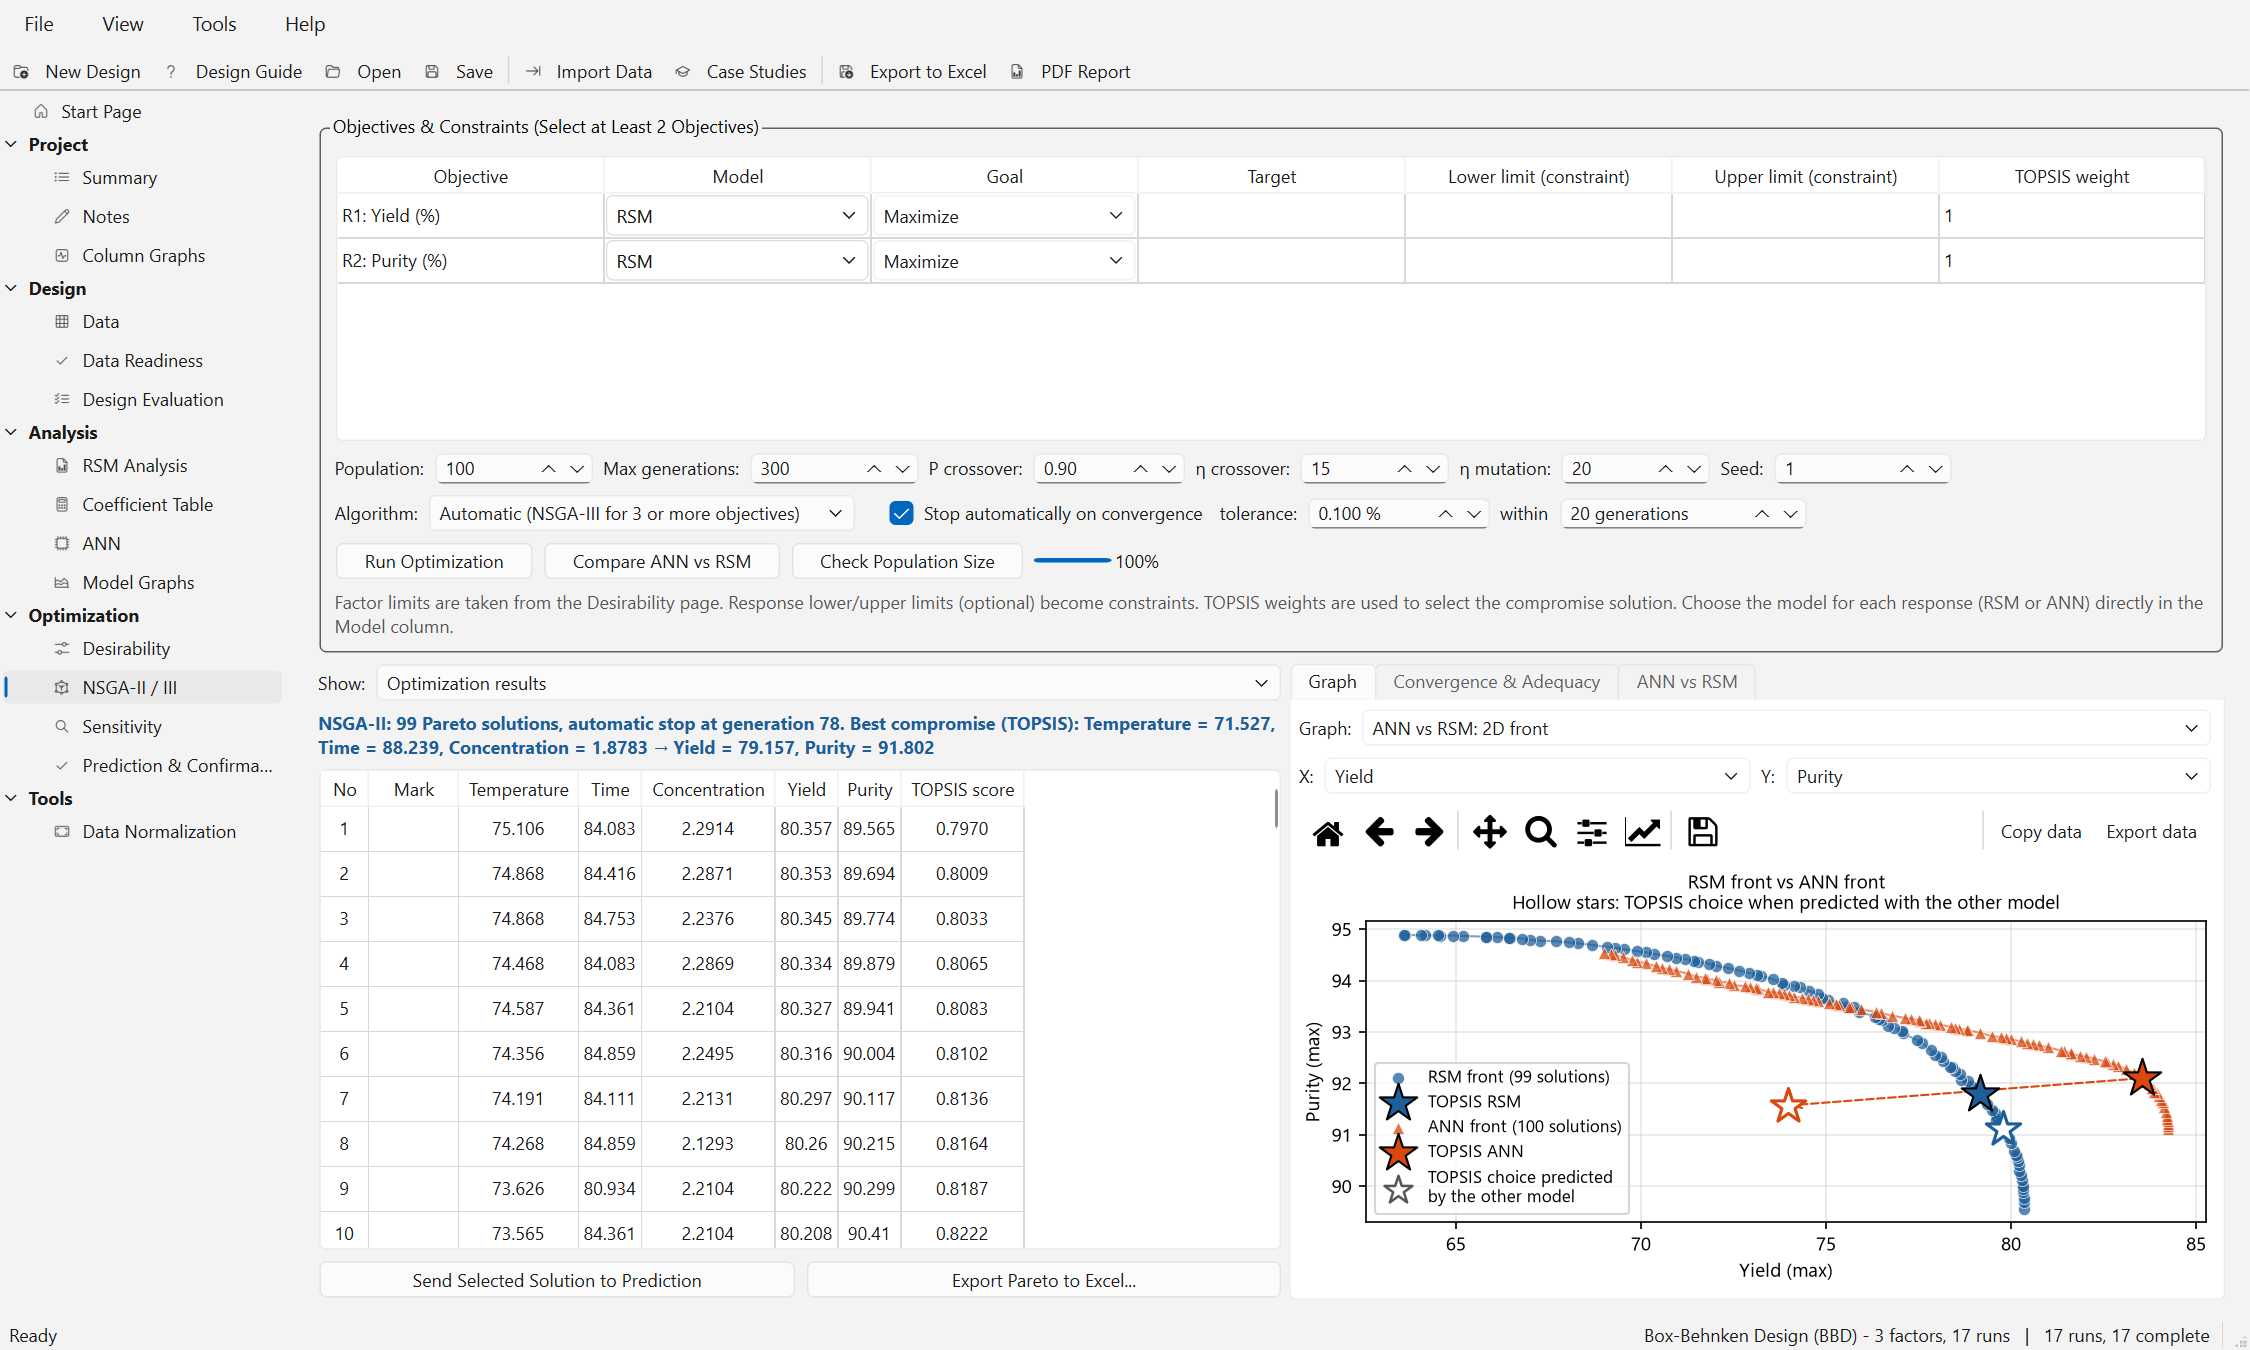
\includegraphics[width=\linewidth]{nsga_compare_front.png}
\caption{\ui{ANN vs RSM: 2D front}: RSM front (blue, 99 solutions) and ANN front (orange, 100 solutions). Hollow stars:
each TOPSIS choice predicted by the other model.}
\label{fig:ch08-cmp-front}
\end{figure}

\begin{figure}[htbp]
\centering
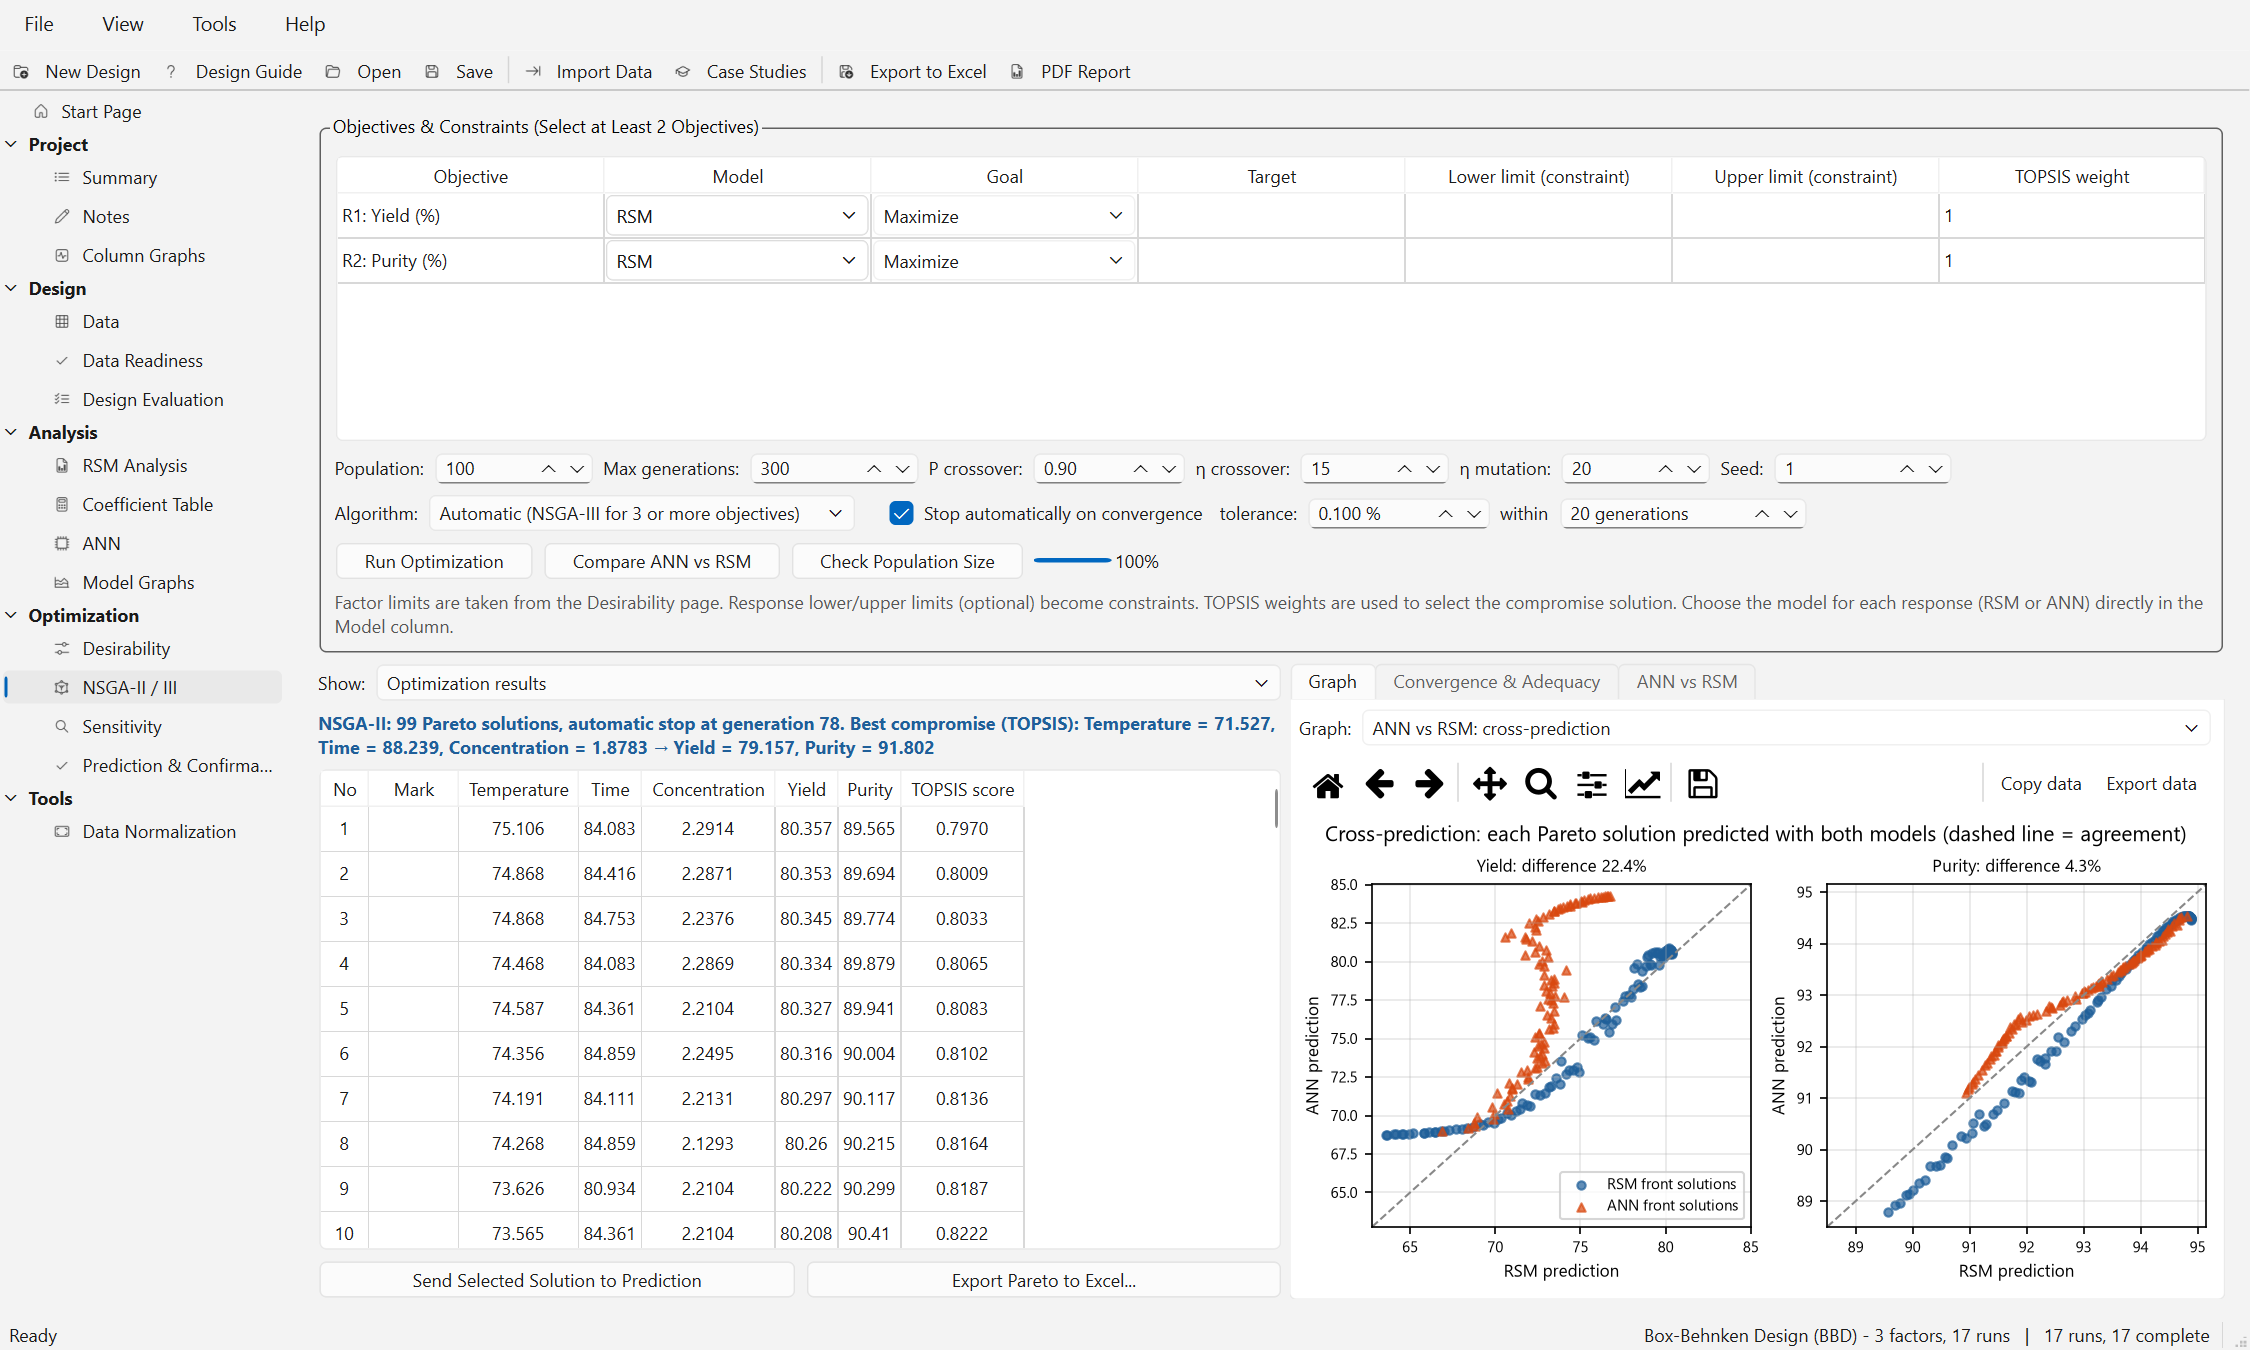
\includegraphics[width=\linewidth]{nsga_compare_cross.png}
\caption{\ui{ANN vs RSM: cross-prediction}: Yield differs by 22.4~\% of its data range on average, Purity by
4.3~\%.}
\label{fig:ch08-cmp-cross}
\end{figure}

\begin{figure}[htbp]
\centering
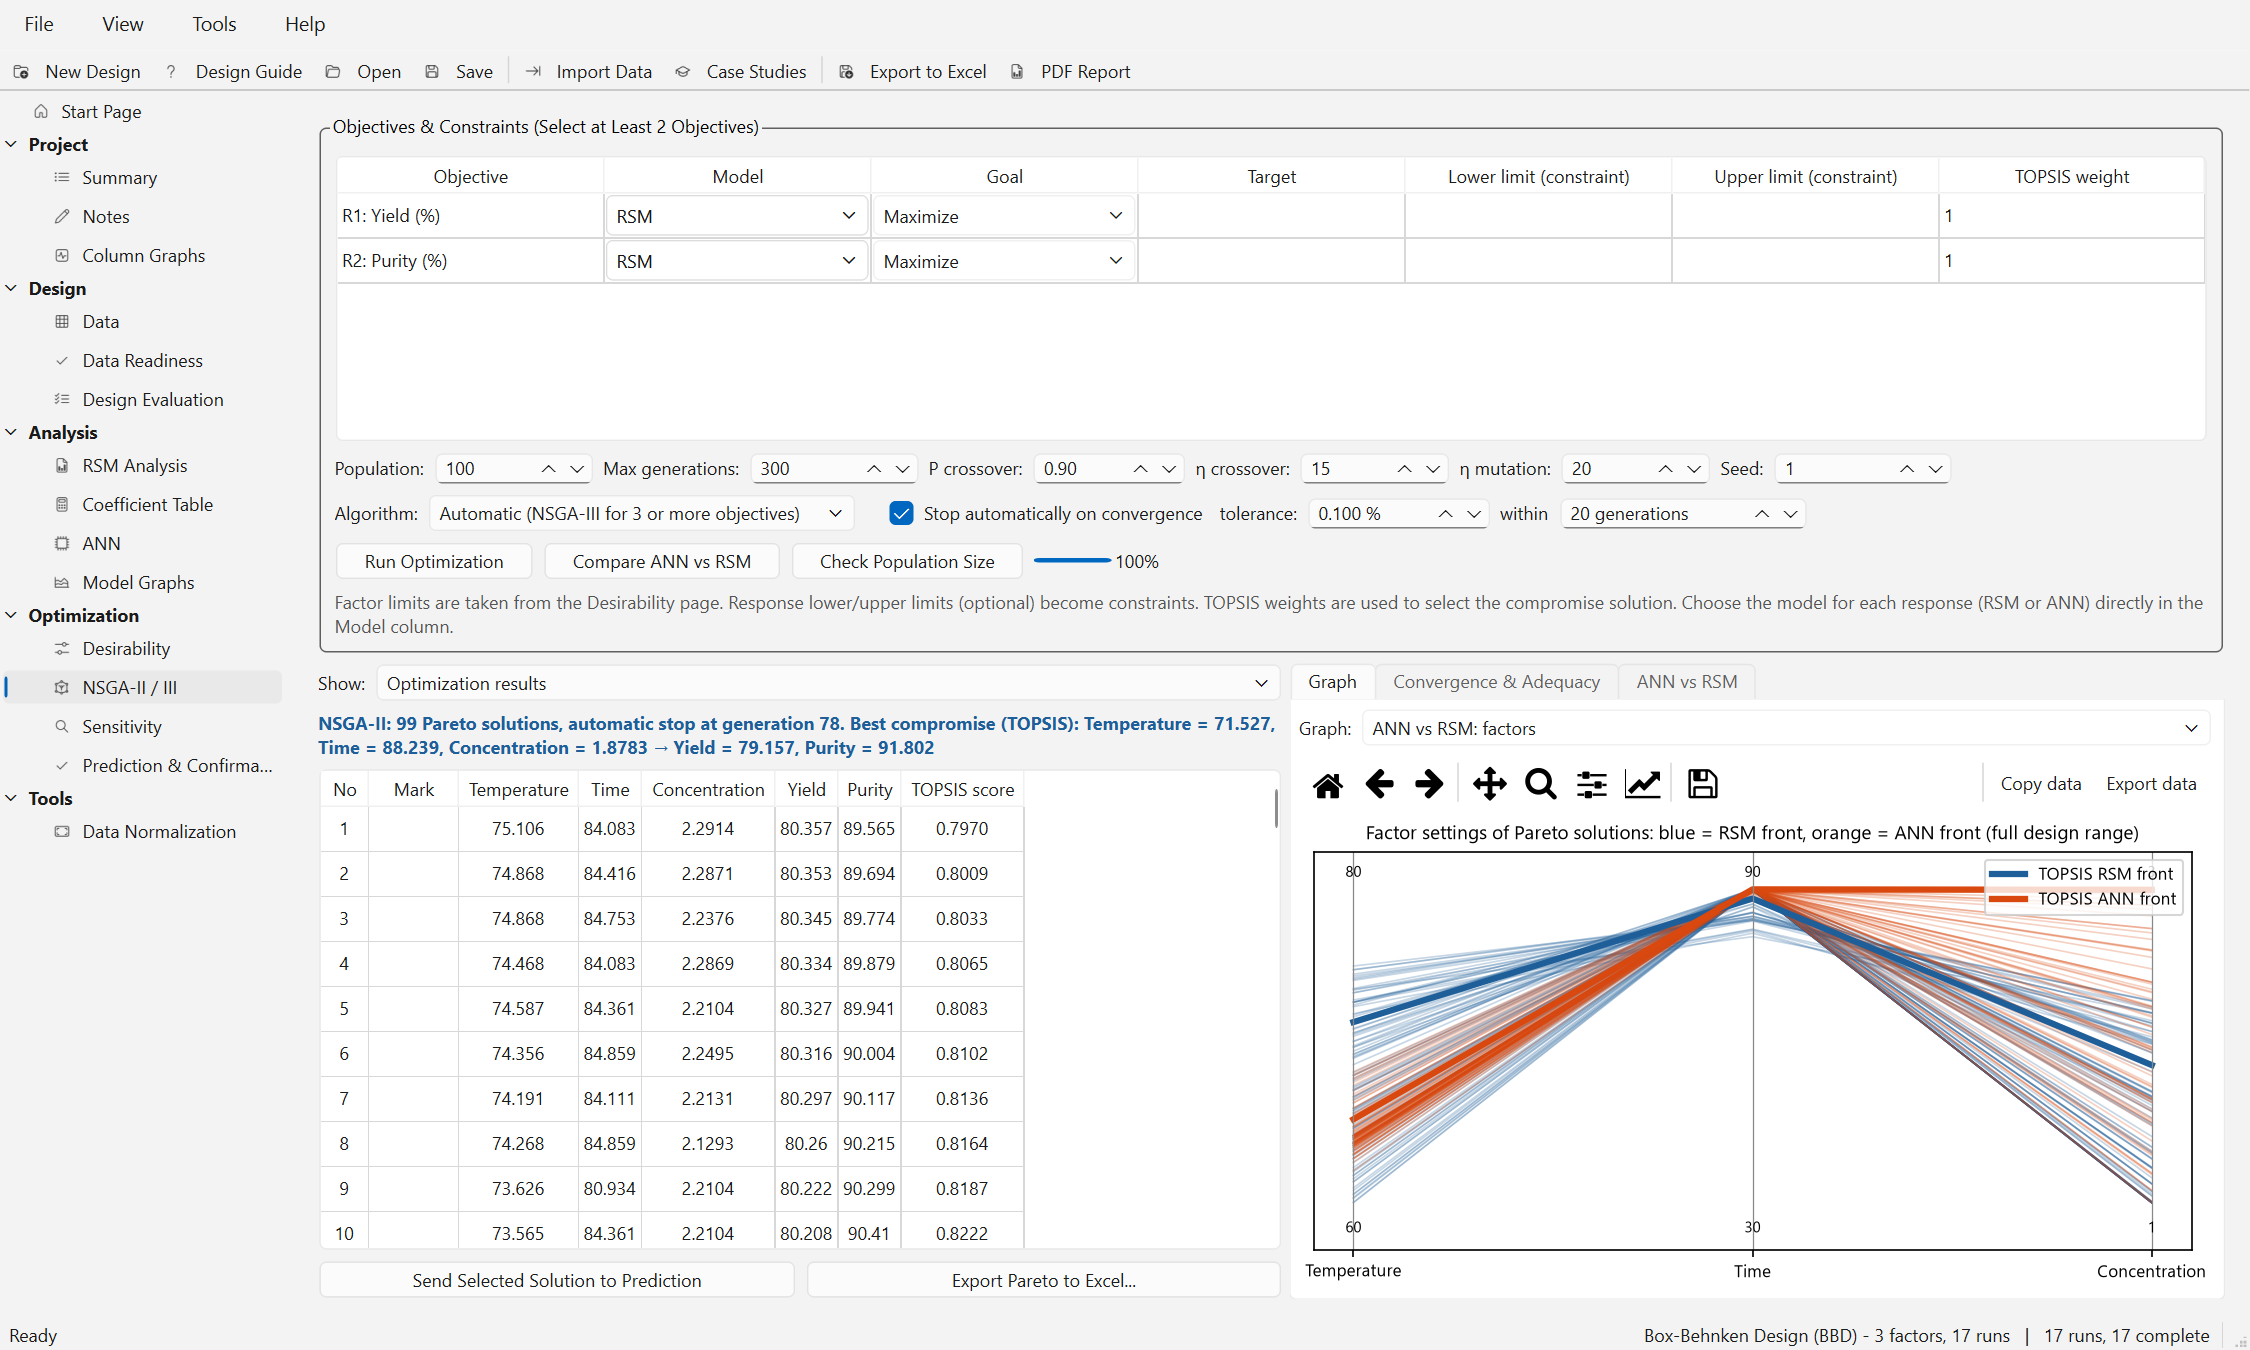
\includegraphics[width=\linewidth]{nsga_compare_factors.png}
\caption{\ui{ANN vs RSM: factors}: the ANN front prefers lower Temperature and higher Concentration than the RSM
front.}
\label{fig:ch08-cmp-factors}
\end{figure}

\begin{figure}[htbp]
\centering
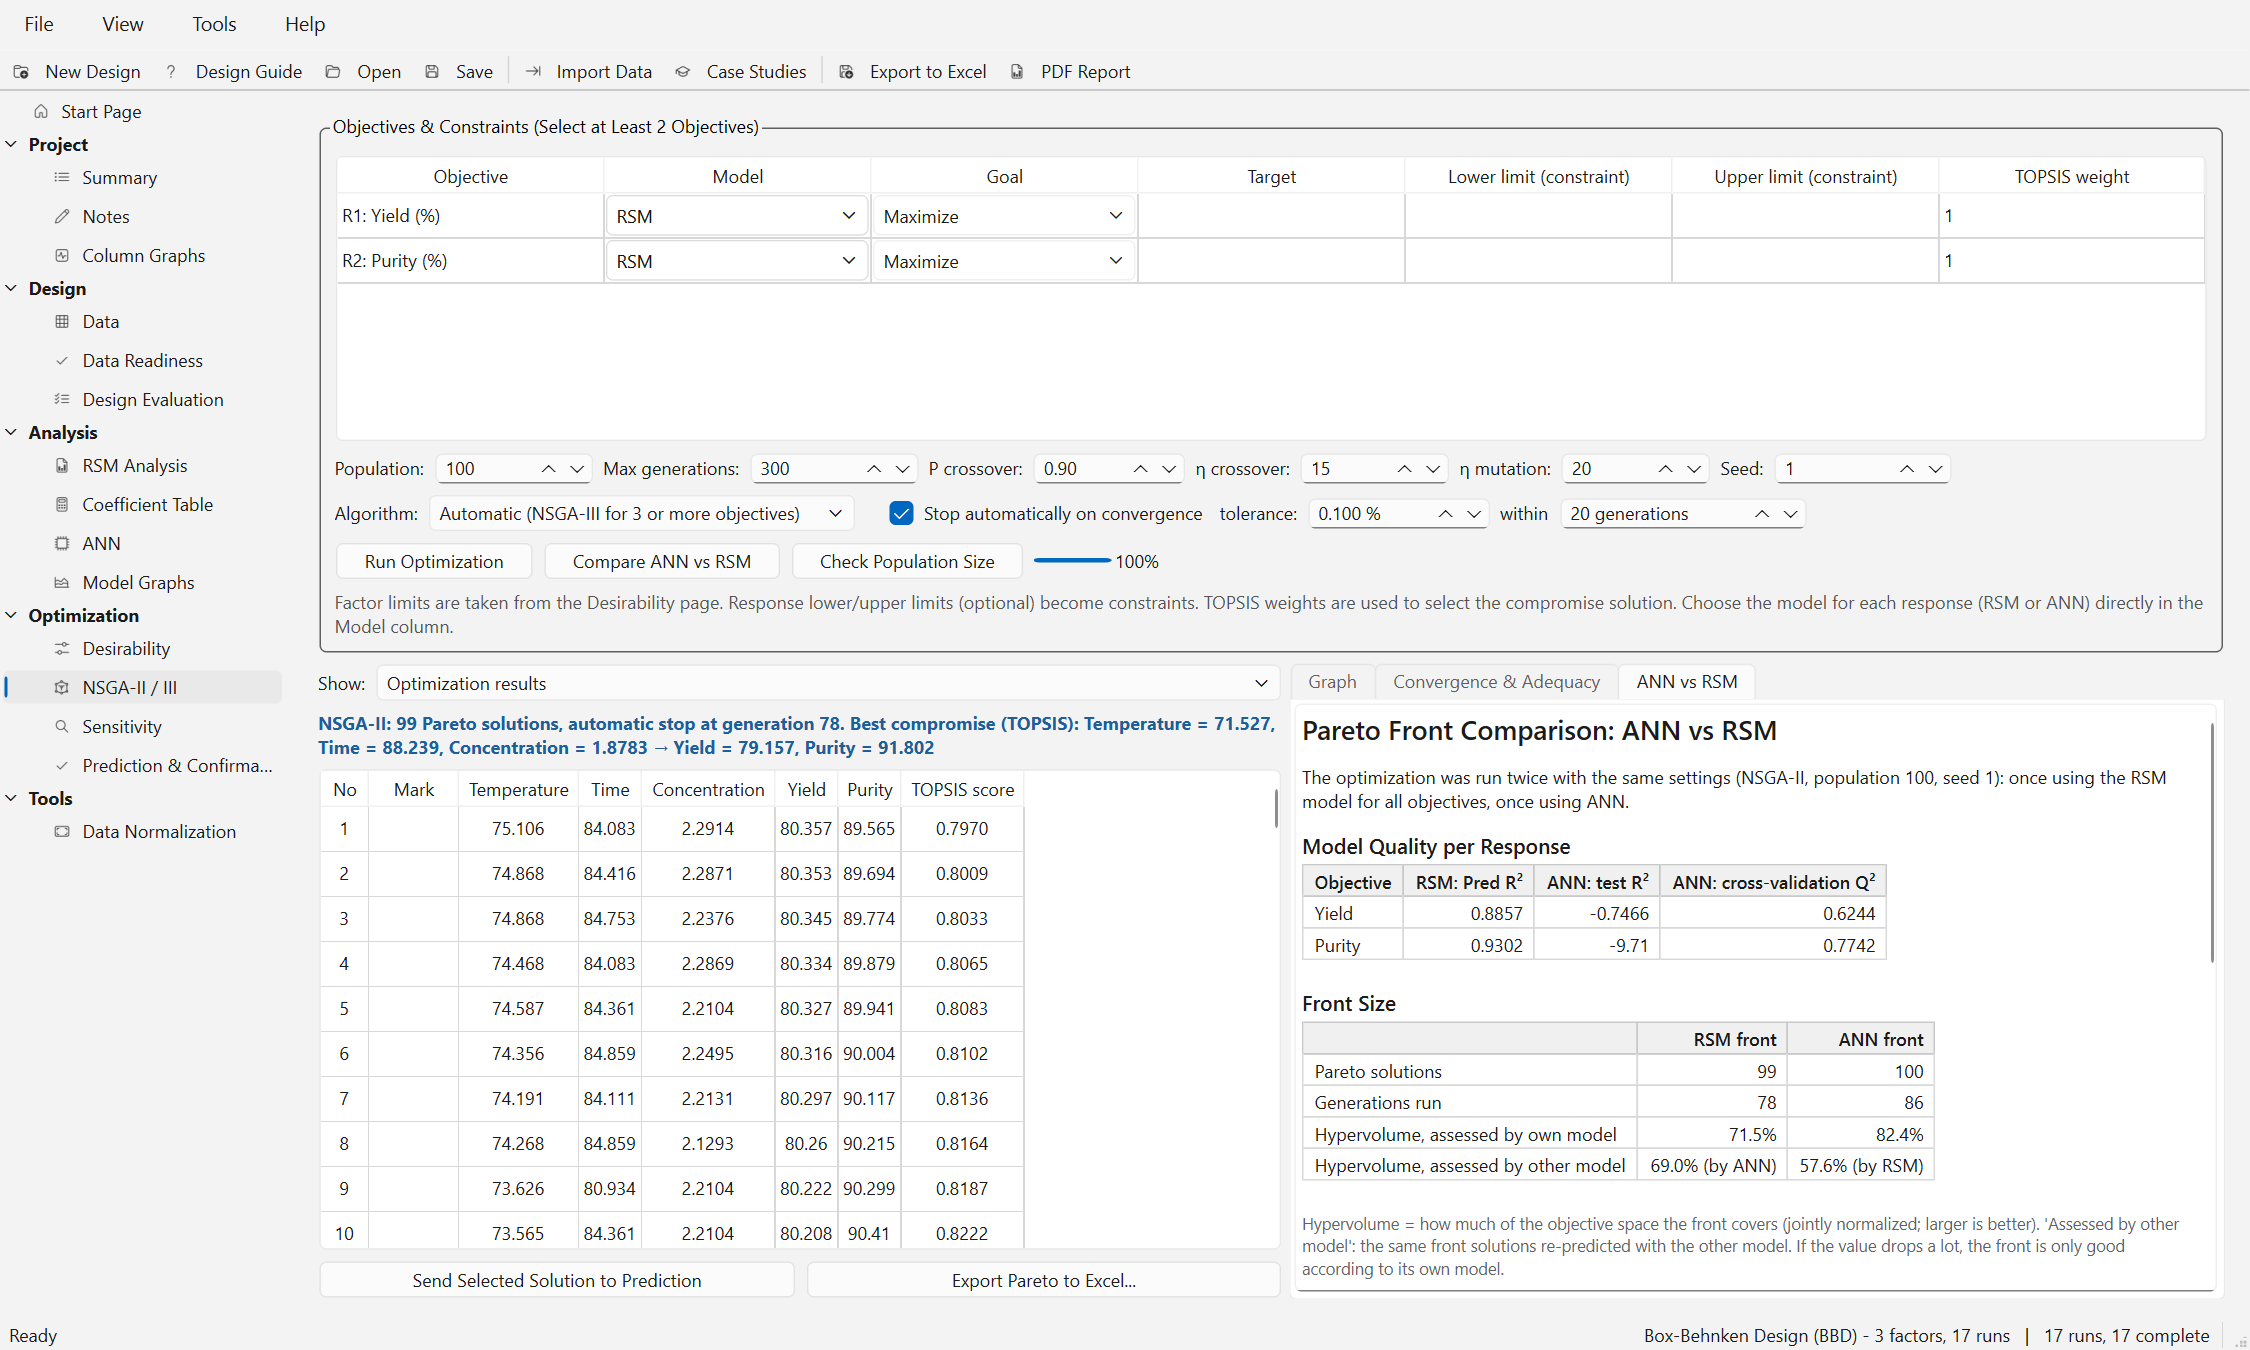
\includegraphics[width=\linewidth]{nsga_compare_report.png}
\caption{\ui{ANN vs RSM} report for the BBD case (upper part).}
\label{fig:ch08-cmp-report}
\end{figure}

The report gives:
\begin{itemize}
  \item Model quality: RSM predicted $R^2$ 0.8857 (Yield) and 0.9302 (Purity); ANN test $R^2$ $-0.7466$ and $-9.71$
        on the single final split (3 test runs each); ANN cross-validation $Q^2$ 0.6244 and 0.7742.
  \item Front size: 99 and 100 solutions, 78 and 86 generations. Hypervolume assessed by the own model 71.5~\% (RSM)
        and 82.4~\% (ANN); assessed by the other model 69.0~\% (RSM front by ANN) and 57.6~\% (ANN front by RSM).
  \item Prediction difference: Yield 22.4~\% mean, 78.0~\% maximum; Purity 4.3~\% mean, 9.9~\% maximum.
  \item TOPSIS choices: RSM front 71.527~°C, 88.239~min, 1.8783~\% (Yield 79.157 by RSM, 79.795 by ANN; Purity
        91.802 / 91.123); ANN front 65.325~°C, 89.999~min, 2.9973~\% (Yield 73.973 by RSM, 83.542 by ANN; Purity
        91.570 / 92.102). Distance $dx=56.0$~\%.
\end{itemize}
The conclusion is red: \ui{The models differ considerably: the largest mean difference of the predictions on the
front is 22.4\%, above the 10\% limit for partial agreement, and the compromise choices are 56\% of the factor range
apart, above the 15\% limit. Do not rely on just one model: make confirmation runs at both TOPSIS points.} It adds that
the ANN front promises the better trade-off by its own model but loses a lot of hypervolume when assessed by RSM,
and it compares the accuracy on new data: RSM mean Pred R² 0.908 against ANN mean cross-validation Q² 0.699 (both
ANNs were found by a search, so the cross-validated value is used).

\textbf{Interpretation.} Check~D fails here, and the reasons are clear. The ANN front reaches a Yield of about 84,
well above the highest observed Yield (78.29), at a corner of the design region (Time 90~min, Concentration 3~\%)
where the BBD has no run: this is extrapolation by a network trained on 17 runs. The RSM model has the better
accuracy on new data (predicted $R^2$ 0.886 and 0.930 against cross-validated $Q^2$ 0.624 and 0.774), and its front
loses little hypervolume when re-assessed by the ANN (71.5 to 69.0~\%). The RSM result is therefore the one to use,
and the disagreement is reported. If the ANN's promise matters, one or two confirmation runs at the ANN TOPSIS
setting decide the question; the RSM 95~\% prediction interval for the mean of three runs there is 72.1--75.8 for
Yield, far from the ANN prediction of 83.5 (see Chapter~\ref{chap:11}).

The single-split test $R^2$ values in the report ($-0.75$ and $-9.71$) are not a fair measure here: with 17 runs
the final split holds only three test runs, and one unusual run dominates $R^2$. Use the cross-validated $Q^2$.

\subsection{Limitations of check D}
Check~D compares two models; agreement does not prove that both are right, it only shows that the conclusion does not
depend on the model type. The prediction differences are measured on the Pareto solutions, which are often at the
edges of the design region where models are least reliable. For POE objectives the range $R_o$ is that of the
predictions, not of data. Finally, both NSGA runs use the same seed, so the comparison is reproducible but reflects one
realization of each front; check~C applies to each of them.

% Chapter 9: Sensitivity and parametric studies
\chapter{Sensitivity and Parametric Studies}\label{chap:9}
\label{ch:09}

Once a model has been fitted and an optimum found, two questions remain: how do the responses change when the
factors move away from the chosen setting, and which factors matter most over the whole region? The page
\ui{Sensitivity} (page title \ui{Sensitivity \& Parametric Study}, group \ui{Optimization}) answers them with four
studies on the fitted models:
\begin{itemize}
  \item \ui{Parametric Study}: response curves when one factor is varied and the others are held at a reference
        point (Section~\ref{sec:ch09-parametric});
  \item \ui{Global Sensitivity}: standardized regression coefficients from a Latin hypercube sample, or Sobol
        indices (Section~\ref{sec:ch09-global});
  \item \ui{Local Sensitivity (Tornado)}: the effect of a small change of each factor around the reference point
        (Section~\ref{sec:ch09-local});
  \item \ui{Pareto Front Trade-off}: which factors drive the trade-off along the last NSGA front
        (Section~\ref{sec:ch09-front}).
\end{itemize}
All studies describe the \emph{model}. They are only as reliable as the model, so check the model first (predicted
$R^2$, diagnostics, and for ANN the cross-validated fit and check~D of Chapter~\ref{chap:8}). The computations are in
\texttt{doe/sensitivity.py}; all work is done in coded units and factor values are shown in actual units.

% ======================================================================================================
\section{Reference point and model}
\label{sec:ch09-reference}
The left group \ui{Reference Point} holds the setting from which the studies start.

\begin{table}[htbp]
\centering
\small
\caption{Controls of the \ui{Reference Point} group.}
\label{tab:ch09-reference}
\begin{tabularx}{\linewidth}{@{}>{\raggedright\arraybackslash}p{3.4cm} >{\raggedright\arraybackslash}X >{\raggedright\arraybackslash}p{3.4cm}@{}}
\toprule
Control & Values & Default \\
\midrule
\ui{Start from:} & \ui{Design center}; \ui{Best desirability solution} (only after a desirability run);
\ui{NSGA: TOPSIS choice} and \ui{NSGA: knee point} (only after an NSGA run); \ui{Custom values} & first available
item \\
\ui{Model:} & \ui{Selected model of each response}, \ui{RSM}, \ui{ANN} & \ui{Selected model of each response} \\
\ui{Factor} / \ui{Value} table & one row per factor (spin box in actual units, or a level list for categoric
factors) & from \ui{Start from:} \\
\bottomrule
\end{tabularx}
\end{table}

\begin{itemize}
  \item Choosing an entry in \ui{Start from:} fills the table. Editing a value switches the entry to \ui{Custom
        values}. The spin boxes are limited to the design range of each factor.
  \item \ui{Selected model of each response} uses the RSM/ANN choice made in the \ui{Model} columns of the
        optimization pages. \ui{RSM} and \ui{ANN} force one model type for all responses; with \ui{ANN}, a response
        without a network keeps its RSM model.
  \item Factors that are not varied in a study stay at the reference values. Mixture components sum to a constant and
        cannot be varied one at a time: they stay at the reference blend (for \ui{Design center}, the centroid of the
        constrained mixture region), and only process and categoric factors are studied.
  \item If the reference point violates component bounds or linear constraints, the message \ui{The reference point
        lies outside the design region (component bounds or constraints). Change the values or choose another start.}
        appears.
\end{itemize}
Every report starts with a line \ui{Reference point (\dots): \dots. Model: \dots.}, so that exported tables always
carry the conditions under which they were computed.

% ======================================================================================================
\section{Parametric study}
\label{sec:ch09-parametric}

\subsection{Purpose}
A parametric study shows how each response changes when one factor is moved over its range while the others are held
fixed. It is the ``one factor at a time'' view of the fitted model around a chosen setting, useful to explain an optimum
and to see which factor creates a conflict between responses.

\subsection{How to use}
\begin{enumerate}
  \item Choose the reference point and the model.
  \item Open the tab \ui{Parametric Study} and choose \ui{Layout:}
        \begin{itemize}
          \item \ui{All factors, one panel each}: every process or categoric factor gets its own panel; all responses
                are drawn in the same panel, each on its own vertical axis.
          \item \ui{One factor, one panel per response}: the factor in \ui{Vary:} is varied from \ui{from} to \ui{to};
                optionally \ui{Curves for:} a second factor adds one curve for each of its \ui{values}.
        \end{itemize}
  \item Set the number of \ui{points} and click \ui{Run}.
\end{enumerate}

\subsection{Options}
\begin{table}[htbp]
\centering
\small
\caption{Options of the parametric study.}
\label{tab:ch09-param-options}
\begin{tabularx}{\linewidth}{@{}>{\raggedright\arraybackslash}p{3.4cm} >{\raggedright\arraybackslash}p{3.6cm} >{\raggedright\arraybackslash}p{2.2cm} >{\raggedright\arraybackslash}X@{}}
\toprule
Option & Values & Default & Meaning \\
\midrule
\ui{Layout:} & all factors / one factor & all factors & See above. \\
\ui{Vary:} & process and categoric factors & first factor & Factor on the horizontal axis (one-factor layout). \\
\ui{from}, \ui{to} & actual units & factor range & Range of the varied numeric factor (one-factor layout; the all-factors
layout always uses the full range). \\
\ui{points} & 3--401 & 11 & Number of evenly spaced values. Categoric factors use each level. \\
\ui{Curves for:} & \ui{(none)} or a factor & \ui{(none)} & Second factor (one-factor layout). \\
\ui{values} & 2--7 & 3 & Number of values of the second factor, evenly spaced over its full range (categoric: all
levels). \\
\bottomrule
\end{tabularx}
\end{table}

\subsection{Output and how to read it}
In the all-factors layout (Figure~\ref{fig:ch09-param-all}) the panels are labelled (a), (b), \dots; the first
response is drawn in black with its axis on the left, further responses in blue, orange, green \dots\ on additional
axes on the right, with matching colors and markers. A dotted vertical line marks the reference value of the varied
factor. The one-factor layout (Figure~\ref{fig:ch09-param-one}) has one panel per response and one curve per value of
the second factor.

Below the graph a table lists the predicted values. Points that violate the bounds or linear constraints of the design
are not predicted; their cells are empty (\ui{Empty cells: the point lies outside the design region (bounds or
constraints).}).

\subsection{Theory as implemented}
For factor $i$ and values $x_i^{(1)},\dots,x_i^{(n)}$ the setting is $\mathbf x=\mathbf x_0$ with component $i$
replaced (and, with curves, component $k$ set to each curve value); each response is predicted by its model.
Nothing is estimated, so the curves carry no uncertainty bands; for confidence bands of an RSM model use the
\ui{One Factor Effect} graph (Chapter~\ref{chap:6}). With an ANN the curves can show wiggles outside the region covered by data.

\subsection{Example}
BBD extraction case, reference point \ui{Best desirability solution} (70.265~°C, 89.781~min, 1.7975~\%), model
\ui{Selected model of each response} (RSM for both), 11 points.

\begin{figure}[htbp]
\centering
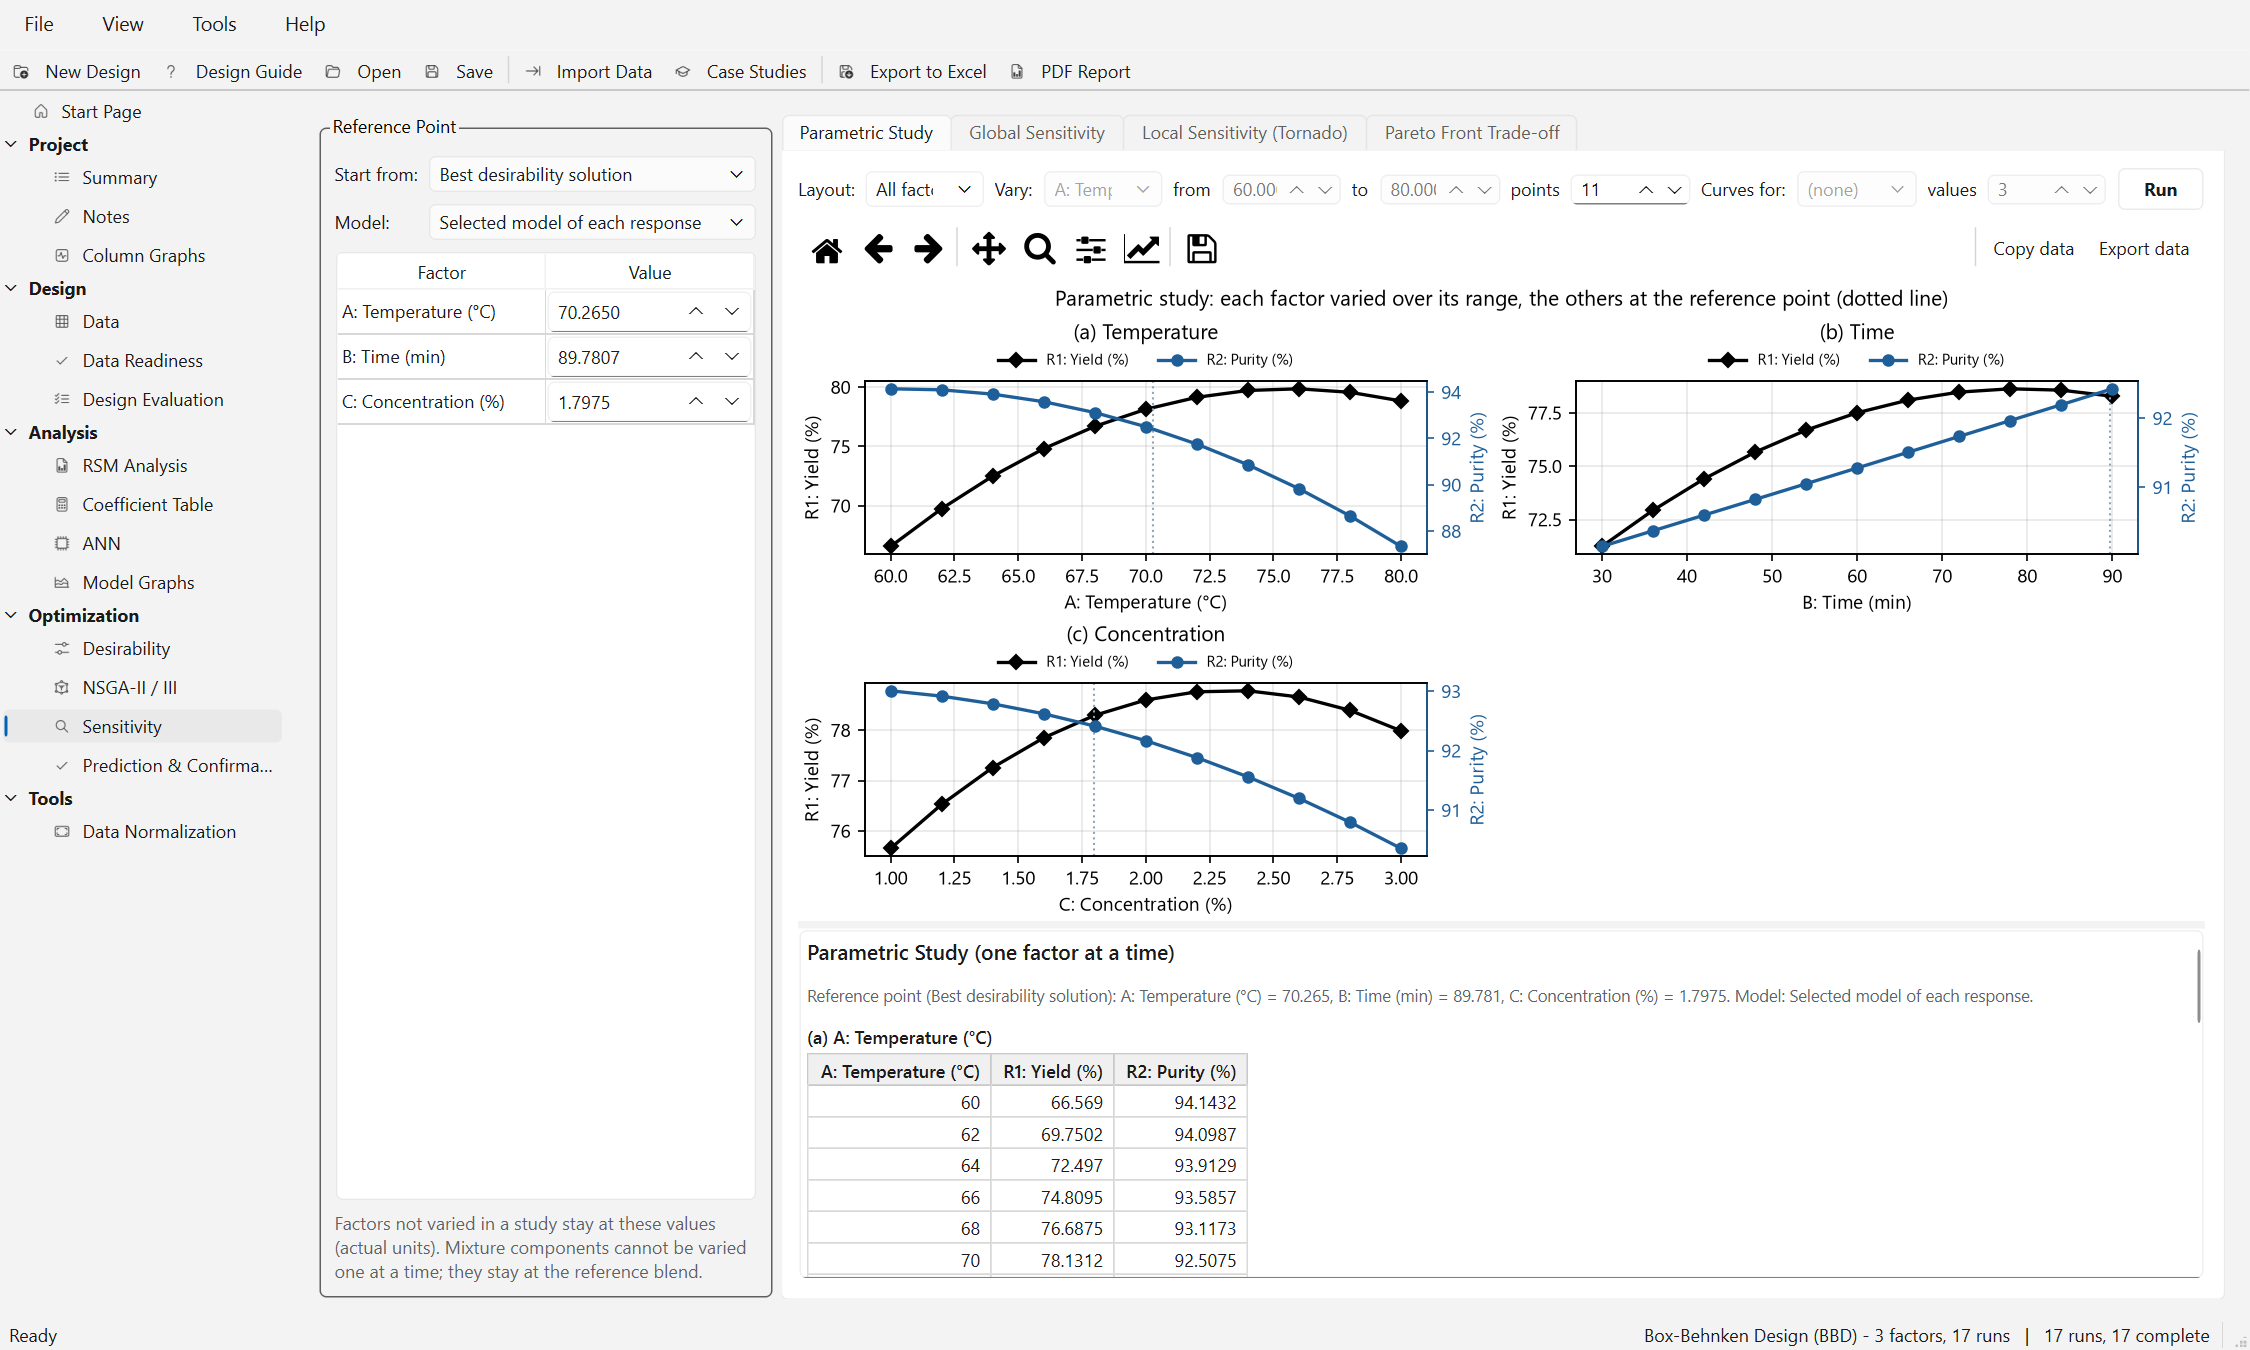
\includegraphics[width=\linewidth]{sens_parametric_all.png}
\caption{Parametric study, layout \ui{All factors, one panel each}: Yield (black, left axis) and Purity (blue, right
axis) against each factor; the dotted line marks the reference value.}
\label{fig:ch09-param-all}
\end{figure}

Panel (a) explains the conflict found by the optimizers: between 60 and 80~°C Yield rises from 66.6 to a maximum of
79.9 near 76~°C and then falls slightly (78.8 at 80~°C), while Purity falls steadily from 94.1 to 87.3. Time (b)
raises both responses up to about 78~min (Yield 78.6), after which Yield decreases slightly while Purity still rises
(92.4 at 90~min), which is why the optima lie at long times. Concentration (c) has a flat Yield maximum near 2.2--2.4~\%
(78.8) and lowers Purity from 93.0 to 90.4.

\begin{figure}[htbp]
\centering
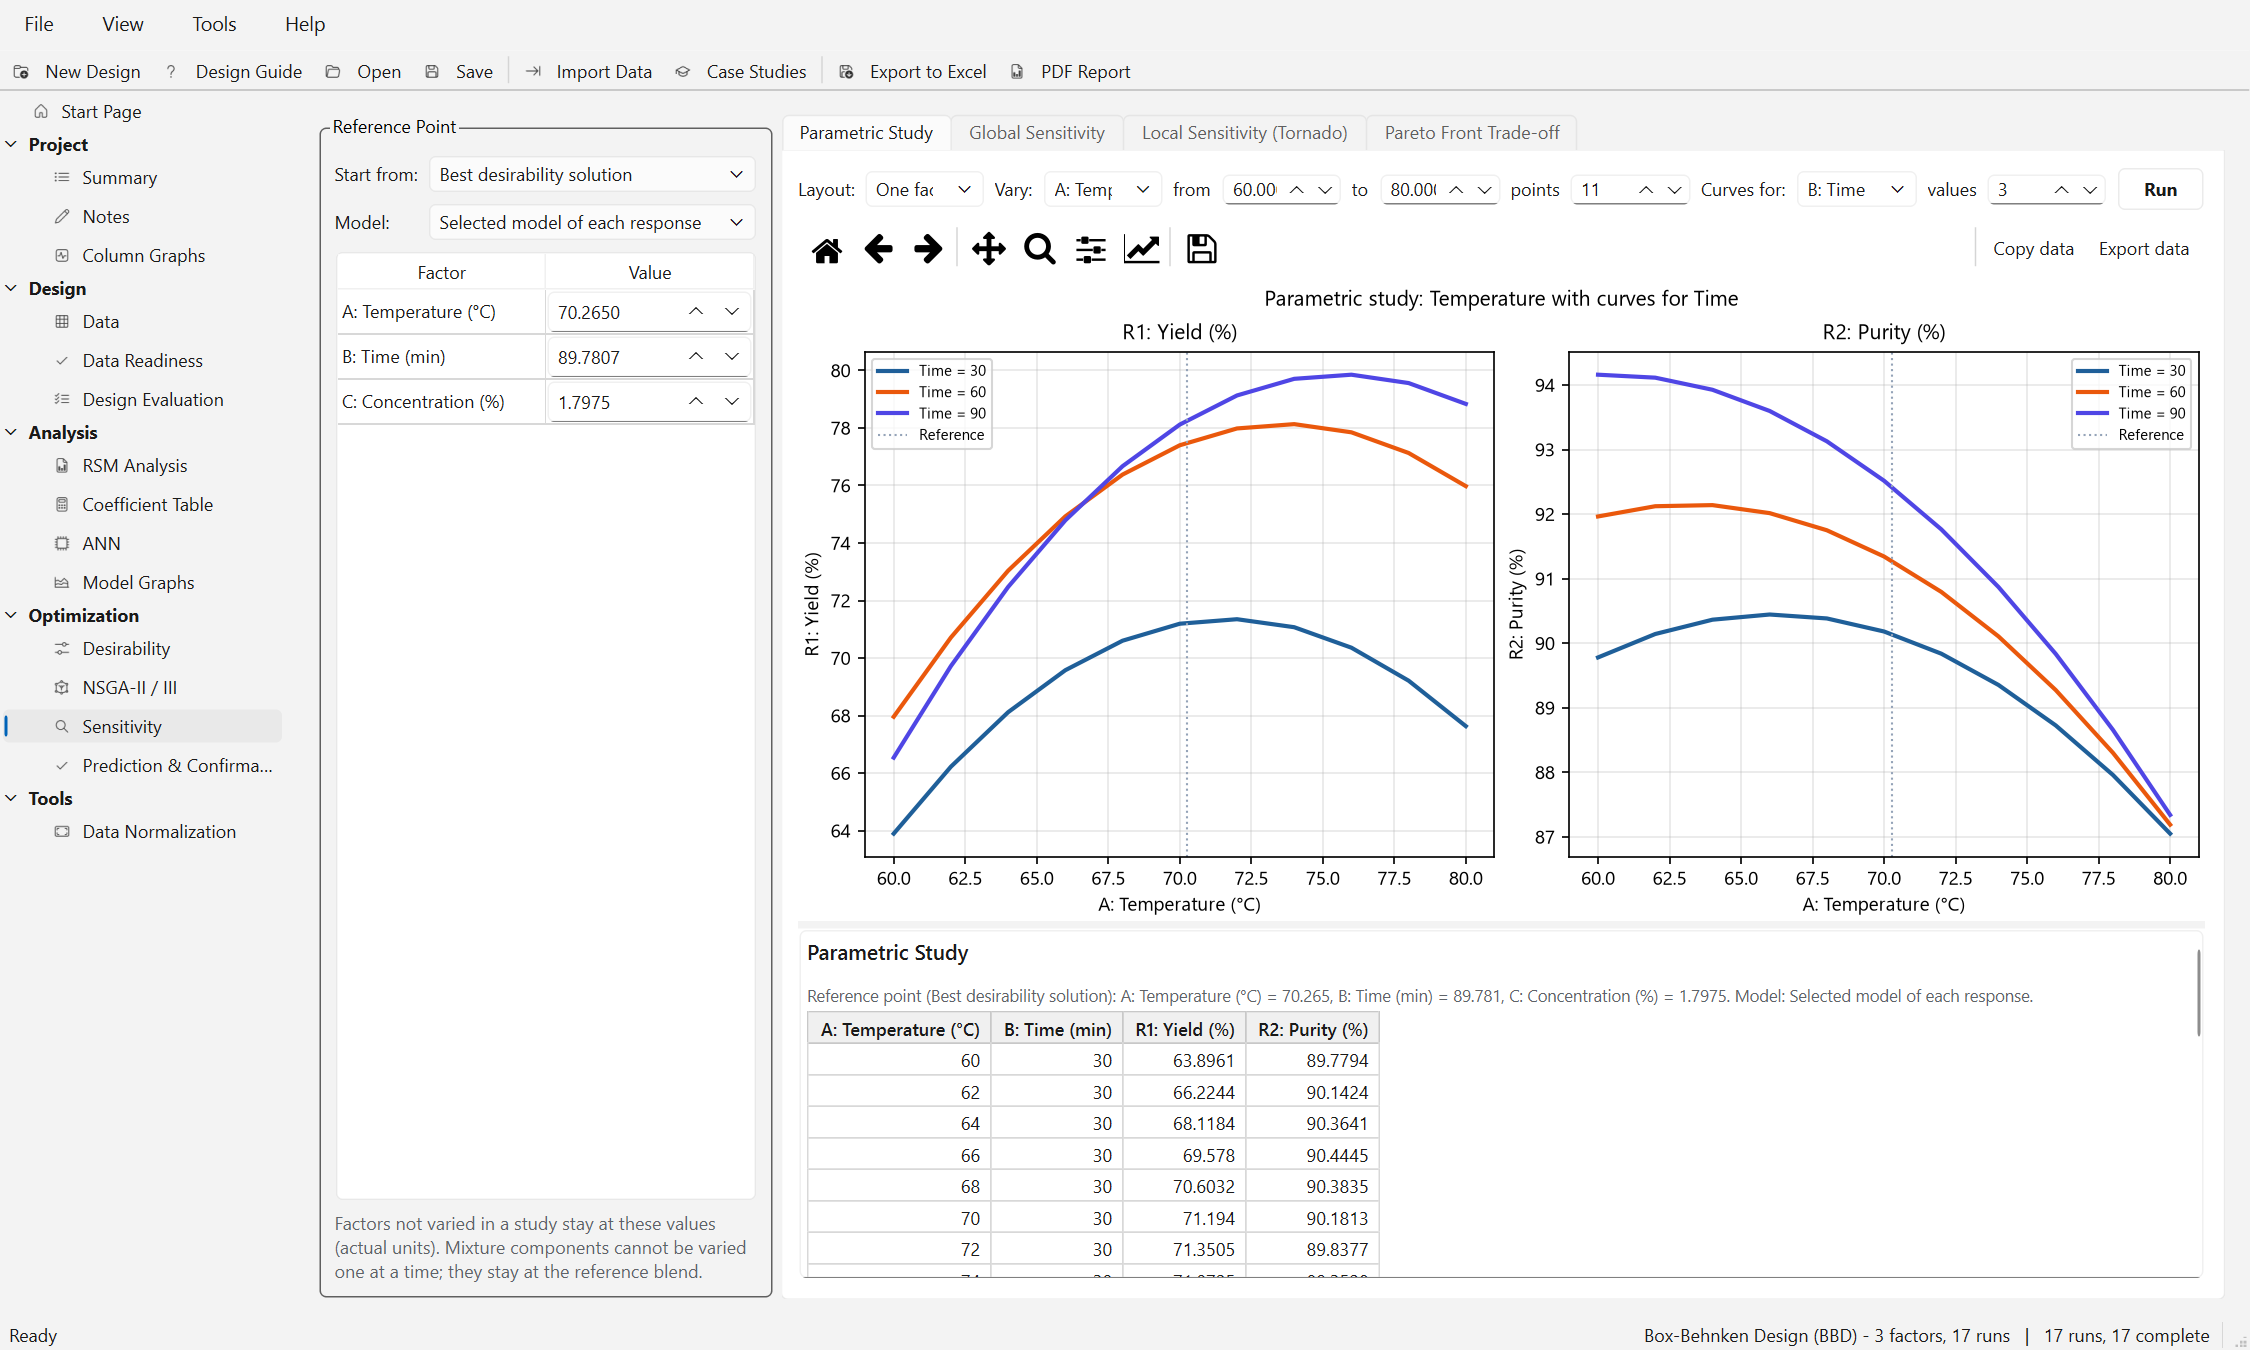
\includegraphics[width=\linewidth]{sens_parametric_one.png}
\caption{Parametric study, layout \ui{One factor, one panel per response}: Temperature varied from 60 to 80~°C with
curves for Time = 30, 60 and 90~min.}
\label{fig:ch09-param-one}
\end{figure}

In Figure~\ref{fig:ch09-param-one} the Yield curves for different times are not parallel: at 30~min Yield peaks at
71.4 near 72~°C, at 90~min it peaks at 79.9 near 76~°C. This is the Temperature $\times$ Time
interaction (AB) of the model.

\textbf{Data export.} \ui{Copy data} and \ui{Export data\dots} export one table per panel (factor values and every
response, also those on the right-hand axes). The report table can be exported with \ui{Export all tables\dots}
(right-click).

% ======================================================================================================
\section{Global sensitivity}
\label{sec:ch09-global}

\subsection{Purpose}
Global sensitivity analysis ranks the factors by their influence over the whole design region, not only near one
point \citep{saltelli2008}. REGEN offers two methods in the tab \ui{Global Sensitivity}, box \ui{Method:}:
\begin{itemize}
  \item \ui{Standardized coefficients (Latin hypercube)}: a linear regression of each response on the factors over a
        space-filling sample. Simple, with a sign and a p-value, but it captures only the linear part.
  \item \ui{Sobol indices (variance-based)}: the share of the response variance caused by each factor, including
        curvature and interactions.
\end{itemize}

\subsection{How to use}
\begin{enumerate}
  \item Choose the reference point (it matters only for factors that are not varied, i.e.\ mixture components) and
        the model.
  \item Choose \ui{Method:} and \ui{Sample size:} (20--65\,536). Switching the method sets the sample size to its
        default: 120 for standardized coefficients and 8192 for Sobol indices.
  \item Click \ui{Run}. The Sobol computation runs in the background; the message \ui{Computing Sobol indices\dots}
        is shown meanwhile.
\end{enumerate}

\subsection{Standardized regression coefficients}
\paragraph{Sampling.} A Latin hypercube sample \citep{mckay1979,stein1987} of $n$ points (default 120, seed 0) is
drawn over the coded ranges of the process and categoric factors; categoric factors take each level with equal share.
Points that violate the design constraints are removed and replaced by points from new Latin hypercubes (seed
$+1000$ per attempt, at most 50 attempts). If fewer than $\max(d+3,10)$ feasible points remain ($d$ = number of
factors), the message \ui{Too few points of the sample satisfy the design constraints.} appears. When constraints
were active the report adds \ui{Sample points that violate the design constraints were replaced by new points.}

\paragraph{Regression.} Each response is predicted at the sample points and regressed by least squares on the
factors,
\begin{equation}
\hat y=b_0+\sum_i b_i x_i\ \ (+\ \text{level indicators of categoric factors}).
\label{eq:ch09-linreg}
\end{equation}
For a numeric factor (and for a two-level categoric factor, through its 0/1 indicator) the standardized coefficient
is
\begin{equation}
\beta_i=b_i\,\frac{s_{x_i}}{s_y},
\label{eq:ch09-beta}
\end{equation}
with $s_{x_i}$ and $s_y$ the sample standard deviations. $\beta_i$ is the change of the response, in standard
deviations, when the factor changes by one standard deviation; its sign gives the direction and $|\beta_i|$ the
strength. The p-value comes from the $t$-test $t=b_i/\text{SE}(b_i)$ with $n-p$ degrees of freedom ($p$ = number of
regression coefficients). A categoric factor with more than two levels has several indicators and no single $\beta$;
it is tested with the partial $F$-test
\begin{equation}
F=\frac{(SSE_\text{reduced}-SSE_\text{full})/q}{SSE_\text{full}/(n-p)},
\label{eq:ch09-ftest}
\end{equation}
where the reduced model omits its $q$ indicators. The report shows \ui{F-test (p)} for such factors.

\paragraph{When $\beta$ is meaningful.} The table ends with \ui{R² of the linear regression}. $\beta$ describes a
response well only when this $R^2$ is high (the page suggests above 0.7). For nearly uncorrelated inputs, as in a Latin
hypercube without constraints, $\sum_i\beta_i^2\approx R^2$ \citep{saltelli2008}, so each $\beta_i^2$ is roughly the
share of variance explained linearly by factor $i$. The remainder $1-R^2$ is curvature and interaction that $\beta$
cannot see; for strongly nonlinear responses use the Sobol indices.

\paragraph{The meaning of the p-values.} The responses at the sample points are model \emph{predictions}, not
measurements. The residual of regression \eqref{eq:ch09-linreg} is therefore the nonlinear part of the model, not
experimental error. The p-value measures how clearly the linear trend stands out from that nonlinear part over this
sample, and it decreases as the sample size grows. Do not present it as evidence that a factor has a real effect on the
process: that evidence comes from the ANOVA of the fitted model (Chapter~\ref{chap:5}). Report $\beta$ with $R^2$, and the p-value
only as a measure of how dominant the linear trend is.

\subsection{Sobol indices}
\paragraph{Definitions.} Let $Y=f(X_1,\dots,X_d)$ with independent inputs and total variance $V=\operatorname{Var}(Y)$.
The first-order and total Sobol indices \citep{sobol2001} are
\begin{equation}
S_{1,i}=\frac{\operatorname{Var}_{X_i}\!\bigl(E[Y\mid X_i]\bigr)}{V},\qquad
S_{T,i}=\frac{E_{\mathbf X_{\sim i}}\!\bigl(\operatorname{Var}[Y\mid\mathbf X_{\sim i}]\bigr)}{V},
\label{eq:ch09-sobol-def}
\end{equation}
where $\mathbf X_{\sim i}$ denotes all inputs except $X_i$. $S_1$ is the share of the variance caused by $X_i$ alone;
$S_T$ also includes all interactions in which $X_i$ takes part. Hence $S_T\ge S_1$, $S_T-S_1$ is the interaction part,
$\sum_i S_{1,i}\le1$ with equality for a purely additive response, and a factor with $S_T\approx0$ has no influence
over the range and can be fixed.

\paragraph{Sampling.} The factors vary uniformly over their full coded ranges; mixture components stay at the reference
point. A scrambled Sobol sequence of dimension $2d$ (seed 0) gives two independent $N\times d$ matrices $\mathbf A$ and
$\mathbf B$ (the first and last $d$ columns). Categoric factors take level $\lfloor uL\rfloor$ for a uniform number $u$
and $L$ levels. $N$ is rounded up to a power of 2 (at least 64), as required for the balance properties of Sobol
sequences. For each factor $i$ the matrix $\mathbf A_B^{(i)}$ equals $\mathbf A$ with column $i$ taken from
$\mathbf B$. The model is evaluated $N(d+2)$ times per response.

\paragraph{Estimators.} The outputs are first centered with $f_0$, the mean of $f(\mathbf A)$ and $f(\mathbf B)$
together; this leaves the estimates unchanged in expectation but lowers their variance. With
$f_A=f(\mathbf A)-f_0$, $f_B=f(\mathbf B)-f_0$, $f_{AB}^{(i)}=f(\mathbf A_B^{(i)})-f_0$ and $\hat V$ the variance of
the $2N$ values $f_A,f_B$,
\begin{align}
\hat S_{1,i}&=\frac{1}{\hat V}\,\frac1N\sum_{r=1}^N f_{B,r}\bigl(f_{AB,r}^{(i)}-f_{A,r}\bigr)
&&\text{\citep{saltelli2010}},\label{eq:ch09-s1}\\
\hat S_{T,i}&=\frac{1}{\hat V}\,\frac1{2N}\sum_{r=1}^N\bigl(f_{A,r}-f_{AB,r}^{(i)}\bigr)^2
&&\text{\citep{jansen1999}}.\label{eq:ch09-st}
\end{align}
These are the estimators recommended by \citet{saltelli2010}.

\paragraph{Confidence intervals.} The $N$ rows are resampled with replacement 200 times (seed 1); the 2.5~\% and
97.5~\% quantiles of the 200 estimates give the 95~\% bootstrap interval shown as error bars and in the columns
\ui{S1 95\% interval} and \ui{ST 95\% interval}. The intervals reflect the Monte Carlo error of the estimate only, not
the uncertainty of the model.

\paragraph{Sample size.} The Monte Carlo error decreases roughly as $1/\sqrt N$. The default $N=8192$ gives errors of
about 0.01 for smooth models (see the validation below); increase $N$ when the intervals are wide or indices near zero
must be distinguished. Small negative estimates of $S_1$ for unimportant factors are Monte Carlo noise.

\paragraph{Constraints.} Sobol indices assume independent inputs, so linear constraints of the design are
\emph{not} applied: the indices describe the whole factor box, including any region excluded by constraints. The report
then warns: \ui{The linear constraints of the design are not applied here, because Sobol indices assume independent
factors; the indices describe the whole factor box.} If the excluded region is large, prefer the standardized
coefficients, which respect the constraints. Sobol indices need at least one process or categoric factor; for a pure
mixture the page says so.

\paragraph{Validation on the Ishigami function.} The Ishigami function \citep{ishigami1990},
\begin{equation}
f(\mathbf x)=\sin x_1+7\sin^2x_2+0.1\,x_3^4\sin x_1,\qquad x_i\sim U(-\pi,\pi),
\label{eq:ch09-ishigami}
\end{equation}
is a standard test case with known indices. The estimators \eqref{eq:ch09-s1}--\eqref{eq:ch09-st} of REGEN
(function \texttt{sobol\_indices}) with the same sampling scheme (scrambled Sobol sequence, seed 0) give
Table~\ref{tab:ch09-ishigami}. With $N=65\,536$ the estimates agree with the analytic values to three decimals:
$S_1=0.314,\ 0.442,\ 0$ and $S_T=0.558,\ 0.442,\ 0.244$. Note that $x_3$ has no first-order effect at all but a
total index of 0.244, entirely through its interaction with $x_1$; a one-factor-at-a-time study at $x_1=0$ would
miss it completely.

\begin{table}[htbp]
\centering
\small
\caption{Sobol indices of the Ishigami function: analytic values and REGEN estimates.}
\label{tab:ch09-ishigami}
\begin{tabular}{@{}lrrrrrr@{}}
\toprule
 & $S_{1,1}$ & $S_{1,2}$ & $S_{1,3}$ & $S_{T,1}$ & $S_{T,2}$ & $S_{T,3}$ \\
\midrule
Analytic & 0.3139 & 0.4424 & 0.0000 & 0.5576 & 0.4424 & 0.2437 \\
$N=1024$ & 0.3223 & 0.4361 & 0.0014 & 0.5560 & 0.4417 & 0.2413 \\
$N=8192$ & 0.3143 & 0.4425 & 0.0002 & 0.5572 & 0.4421 & 0.2435 \\
$N=65\,536$ & 0.3139 & 0.4424 & 0.0000 & 0.5576 & 0.4424 & 0.2437 \\
\bottomrule
\end{tabular}
\end{table}

\subsection{Output and how to read it}
For standardized coefficients the graph shows horizontal bars of $\beta$ per factor (one color per response) and the
table \ui{Decision variable (range)} with \ui{$\beta$ (p-value)} per response, green when $p<0.05$, and the row
\ui{R² of the linear regression}. For Sobol indices the graph has one panel per response with bars for \ui{First order
S1} and \ui{Total ST} and 95~\% bootstrap error bars; the table per response lists \ui{S1}, \ui{S1 95\% interval},
\ui{ST}, \ui{ST 95\% interval} and \ui{ST − S1}, sorted by $S_T$, followed by \ui{Sum of S1 = \dots\ (1 = purely
additive response; the rest is due to interactions).} The note states $N$ and the number of model evaluations.

\subsection{Example}
BBD case, same reference point and model as above.

\begin{figure}[htbp]
\centering
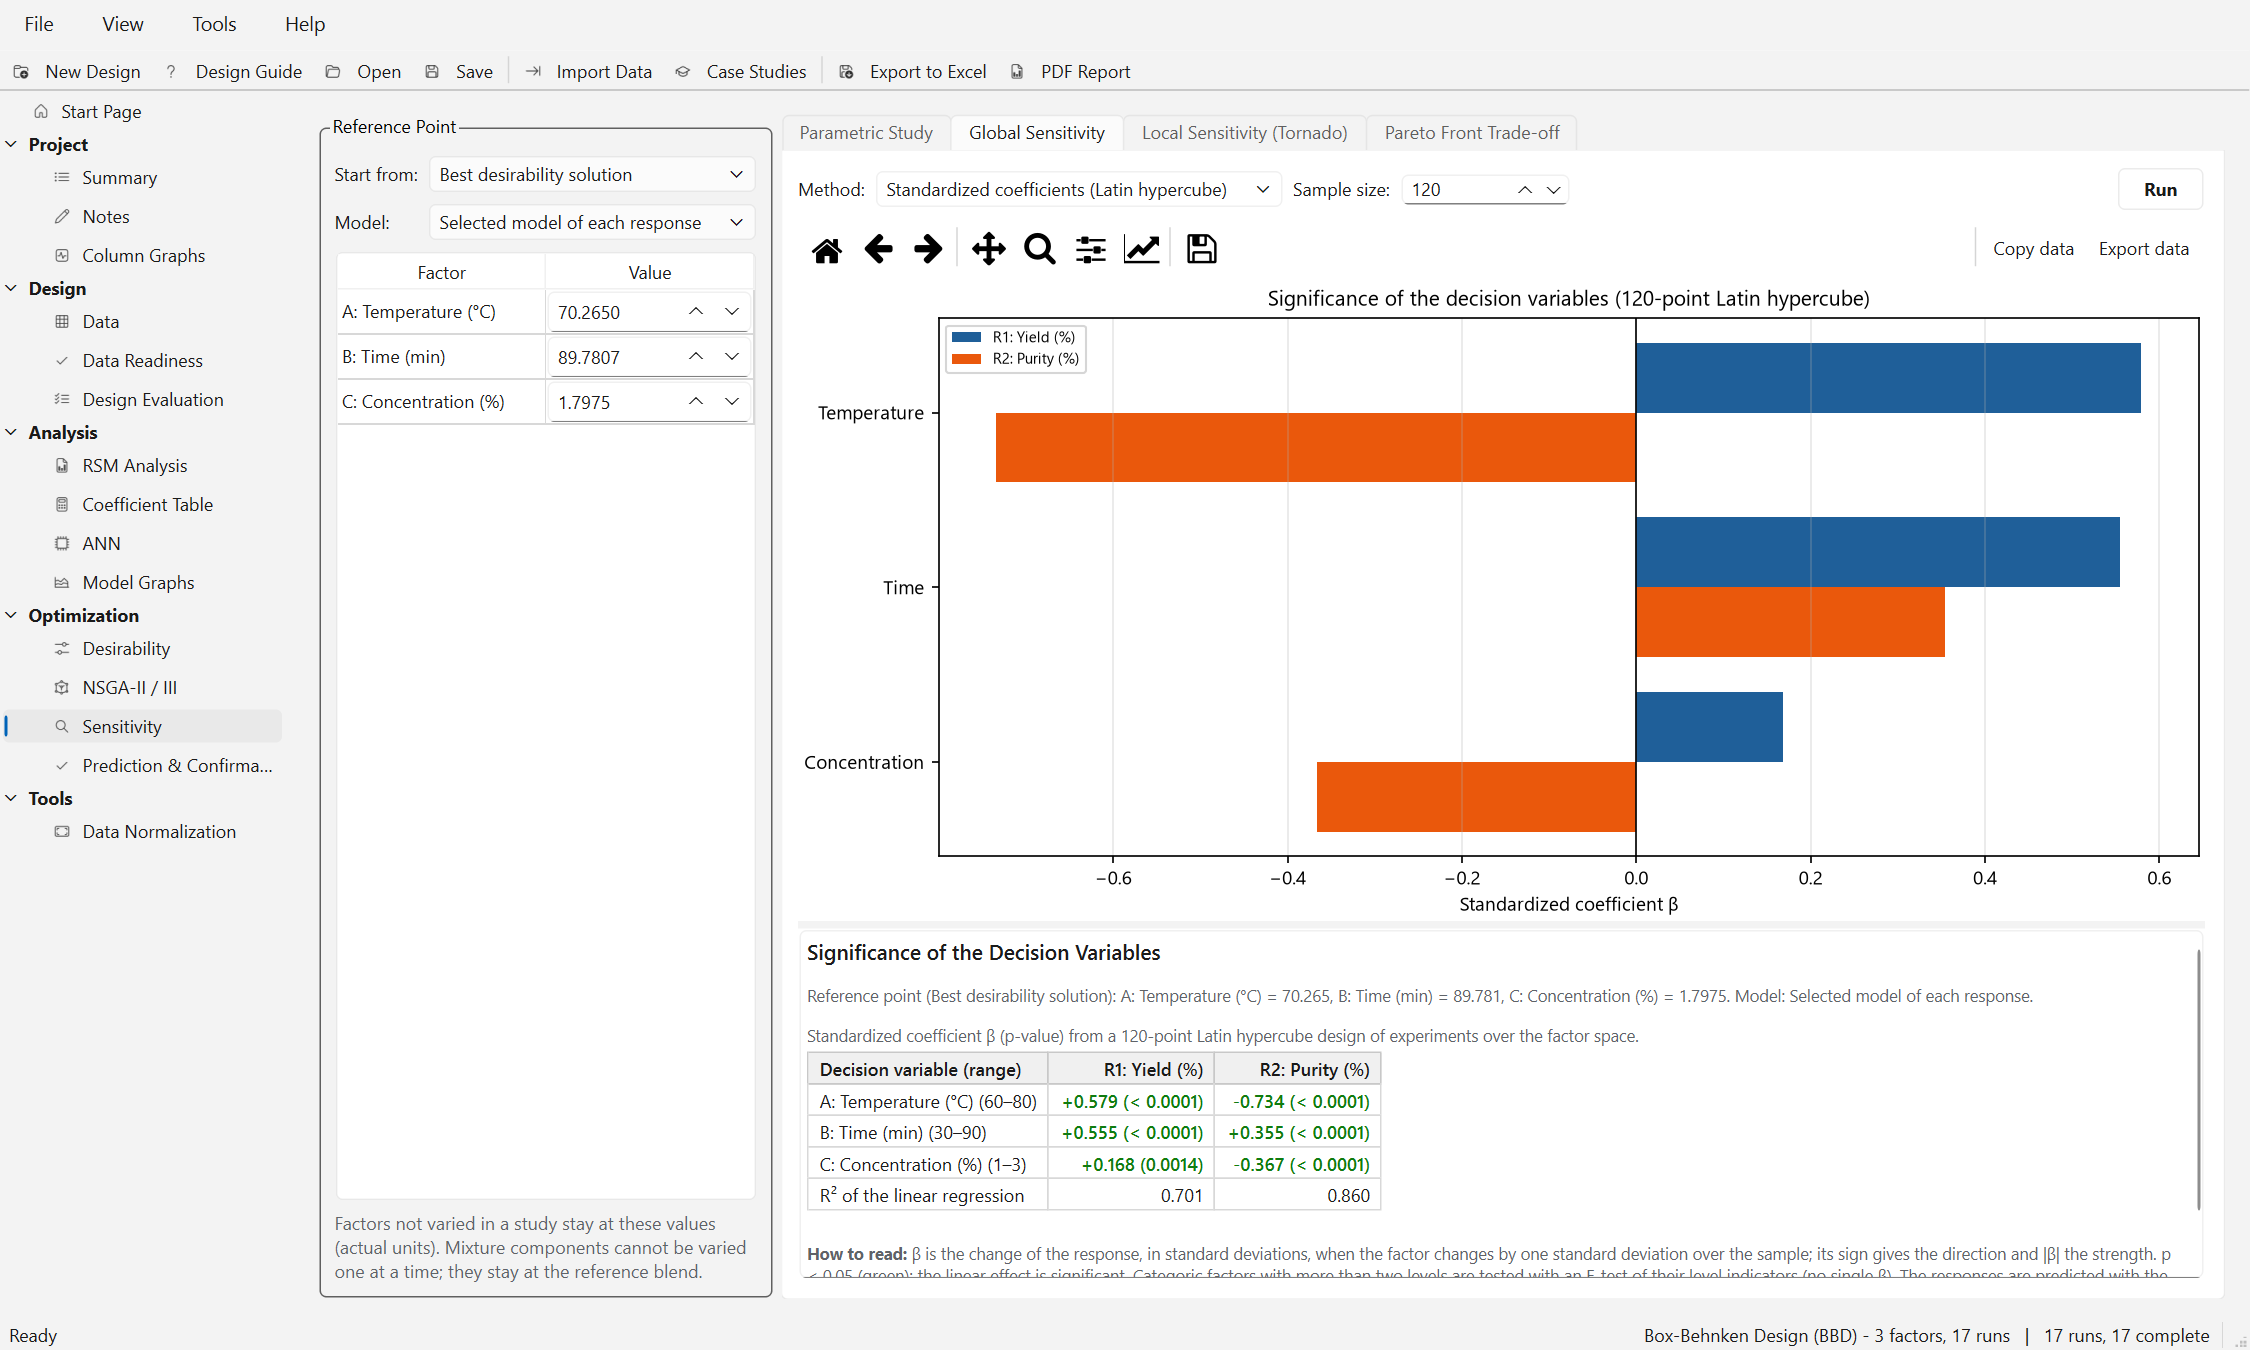
\includegraphics[width=\linewidth]{sens_src.png}
\caption{Standardized regression coefficients from a 120-point Latin hypercube (BBD case).}
\label{fig:ch09-src}
\end{figure}

Standardized coefficients (Figure~\ref{fig:ch09-src}, $n=120$): Yield: Temperature $+0.579$, Time $+0.555$,
Concentration $+0.168$ ($p=0.0014$); Purity: Temperature $-0.734$, Time $+0.355$, Concentration $-0.367$; all other
$p<0.0001$. $R^2$ of the linear regression is 0.701 (Yield) and 0.860 (Purity). For Yield the sum of $\beta^2$ is
0.671, close to $R^2$, and 30~\% of the variance is not linear: the strong curvature of Yield in Temperature
($A^2$ term) is invisible to $\beta$.

\begin{figure}[htbp]
\centering
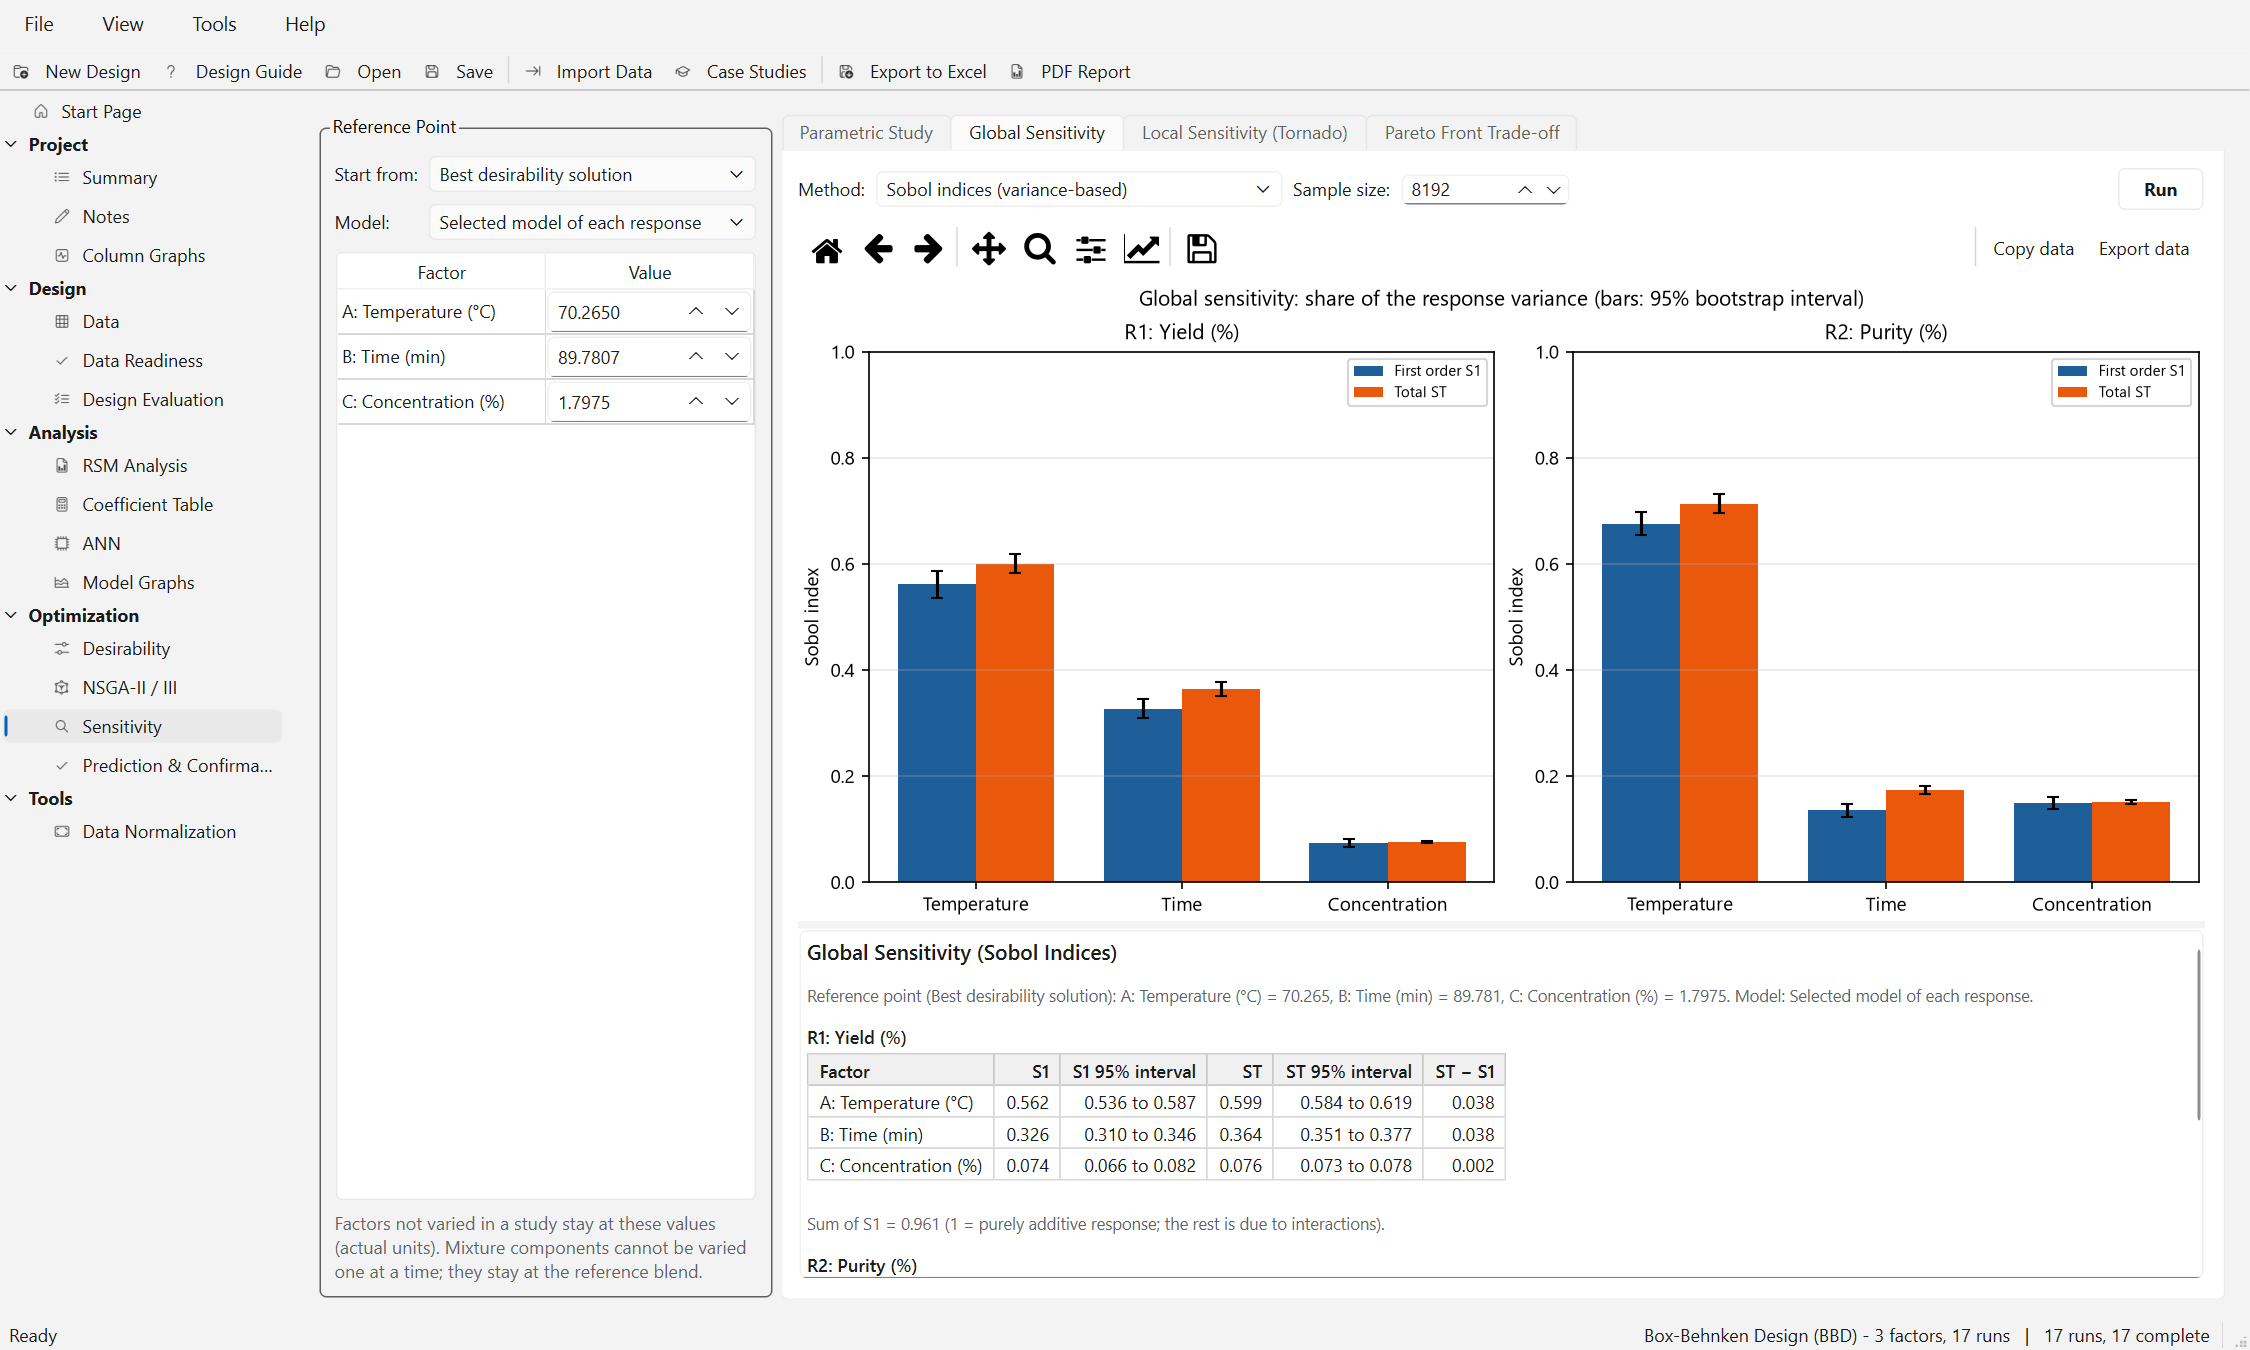
\includegraphics[width=\linewidth]{sens_sobol.png}
\caption{Sobol indices with 95~\% bootstrap intervals, $N=8192$ (40\,960 model evaluations per response).}
\label{fig:ch09-sobol}
\end{figure}

Sobol indices (Figure~\ref{fig:ch09-sobol}, $N=8192$) are given in Table~\ref{tab:ch09-sobol-bbd}. For Yield,
Temperature dominates ($S_T=0.599$) and Time is clearly second ($S_T=0.364$), whereas the linear $\beta$ ranked the two
almost equal: the Sobol index includes the curved Temperature effect. The sums of $S_1$ are 0.961 for both responses,
so about 4~\% of the variance comes from interactions, mainly Temperature $\times$ Time ($S_T-S_1=0.038$ for both).
Concentration matters little for Yield ($S_T=0.076$) but more for Purity (0.151).

\begin{table}[htbp]
\centering
\small
\caption{Sobol indices of the BBD case (RSM models, $N=8192$), with 95~\% bootstrap intervals.}
\label{tab:ch09-sobol-bbd}
\begin{tabular}{@{}llllll@{}}
\toprule
Response & Factor & $S_1$ & 95~\% interval & $S_T$ & 95~\% interval \\
\midrule
Yield & Temperature & 0.562 & 0.536--0.587 & 0.599 & 0.584--0.619 \\
      & Time & 0.326 & 0.310--0.346 & 0.364 & 0.351--0.377 \\
      & Concentration & 0.074 & 0.066--0.082 & 0.076 & 0.073--0.078 \\
Purity & Temperature & 0.676 & 0.654--0.698 & 0.714 & 0.696--0.731 \\
      & Time & 0.136 & 0.123--0.148 & 0.174 & 0.166--0.181 \\
      & Concentration & 0.149 & 0.138--0.161 & 0.151 & 0.147--0.155 \\
\bottomrule
\end{tabular}
\end{table}

\textbf{Data export.} Graph: \ui{Copy data} / \ui{Export data\dots}; report: right-click, \ui{Export all
tables\dots}.

% ======================================================================================================
\section{Local sensitivity (tornado chart)}
\label{sec:ch09-local}

\subsection{Purpose}
The tab \ui{Local Sensitivity (Tornado)} shows how much each response changes when each factor is moved a small step
up and down from the reference point. It answers practical questions about the chosen setting: which factor must be
controlled most tightly, and how much does the response suffer from a small deviation?

\subsection{How to use}
Choose the reference point and model, set \ui{Change each factor by $\pm$} (1--50~\% of the range, default 10~\%) and
click \ui{Run}.

\subsection{Theory as implemented}
For a numeric factor $i$ with coded range $[l_i,u_i]$, reference value $x_{0,i}$ and step $\delta$,
\begin{equation}
x_i^\text{lo}=\max\bigl(l_i,\;x_{0,i}-\delta(u_i-l_i)\bigr),\qquad
x_i^\text{hi}=\min\bigl(u_i,\;x_{0,i}+\delta(u_i-l_i)\bigr),
\label{eq:ch09-steps}
\end{equation}
so a step that would leave the range is clipped at the bound. The responses $y^\text{lo}$ and $y^\text{hi}$ are
predicted with all other factors at the reference; a point that violates the design constraints is not predicted. The
\emph{swing} is the signed difference $y^\text{hi}-y^\text{lo}$ and the \emph{normalized sensitivity} is
\begin{equation}
S_i^\text{norm}=\frac{y^\text{hi}-y^\text{lo}}{x_i^\text{hi}-x_i^\text{lo}}\cdot\frac{R_i}{|y_0|},
\label{eq:ch09-normsens}
\end{equation}
with the factor values and the range $R_i$ in actual units and $y_0$ the response at the reference point. It is the
relative change of the response for a change of the factor over its whole range, at the local slope; it is
dimensionless and can be compared between factors and responses (it is not shown when $y_0=0$). For a categoric factor
all levels are evaluated; ``low'' is the level with the smallest and ``high'' the level with the largest response, and
no normalized sensitivity is given.

The result is valid only near the reference point. At an optimum the slopes of the optimized responses are close to
zero by definition, so a tornado chart at the optimum mainly shows curvature and the slopes of the other responses.

\subsection{Output}
One panel per response with horizontal bars from the reference value $y_0$ (black line) to the response at the low
setting (blue) and at the high setting (orange), sorted with the largest $|$swing$|$ on top. The table per response
gives the low and high settings, the responses, the swing and the normalized sensitivity.

\subsection{Example}
\begin{figure}[htbp]
\centering
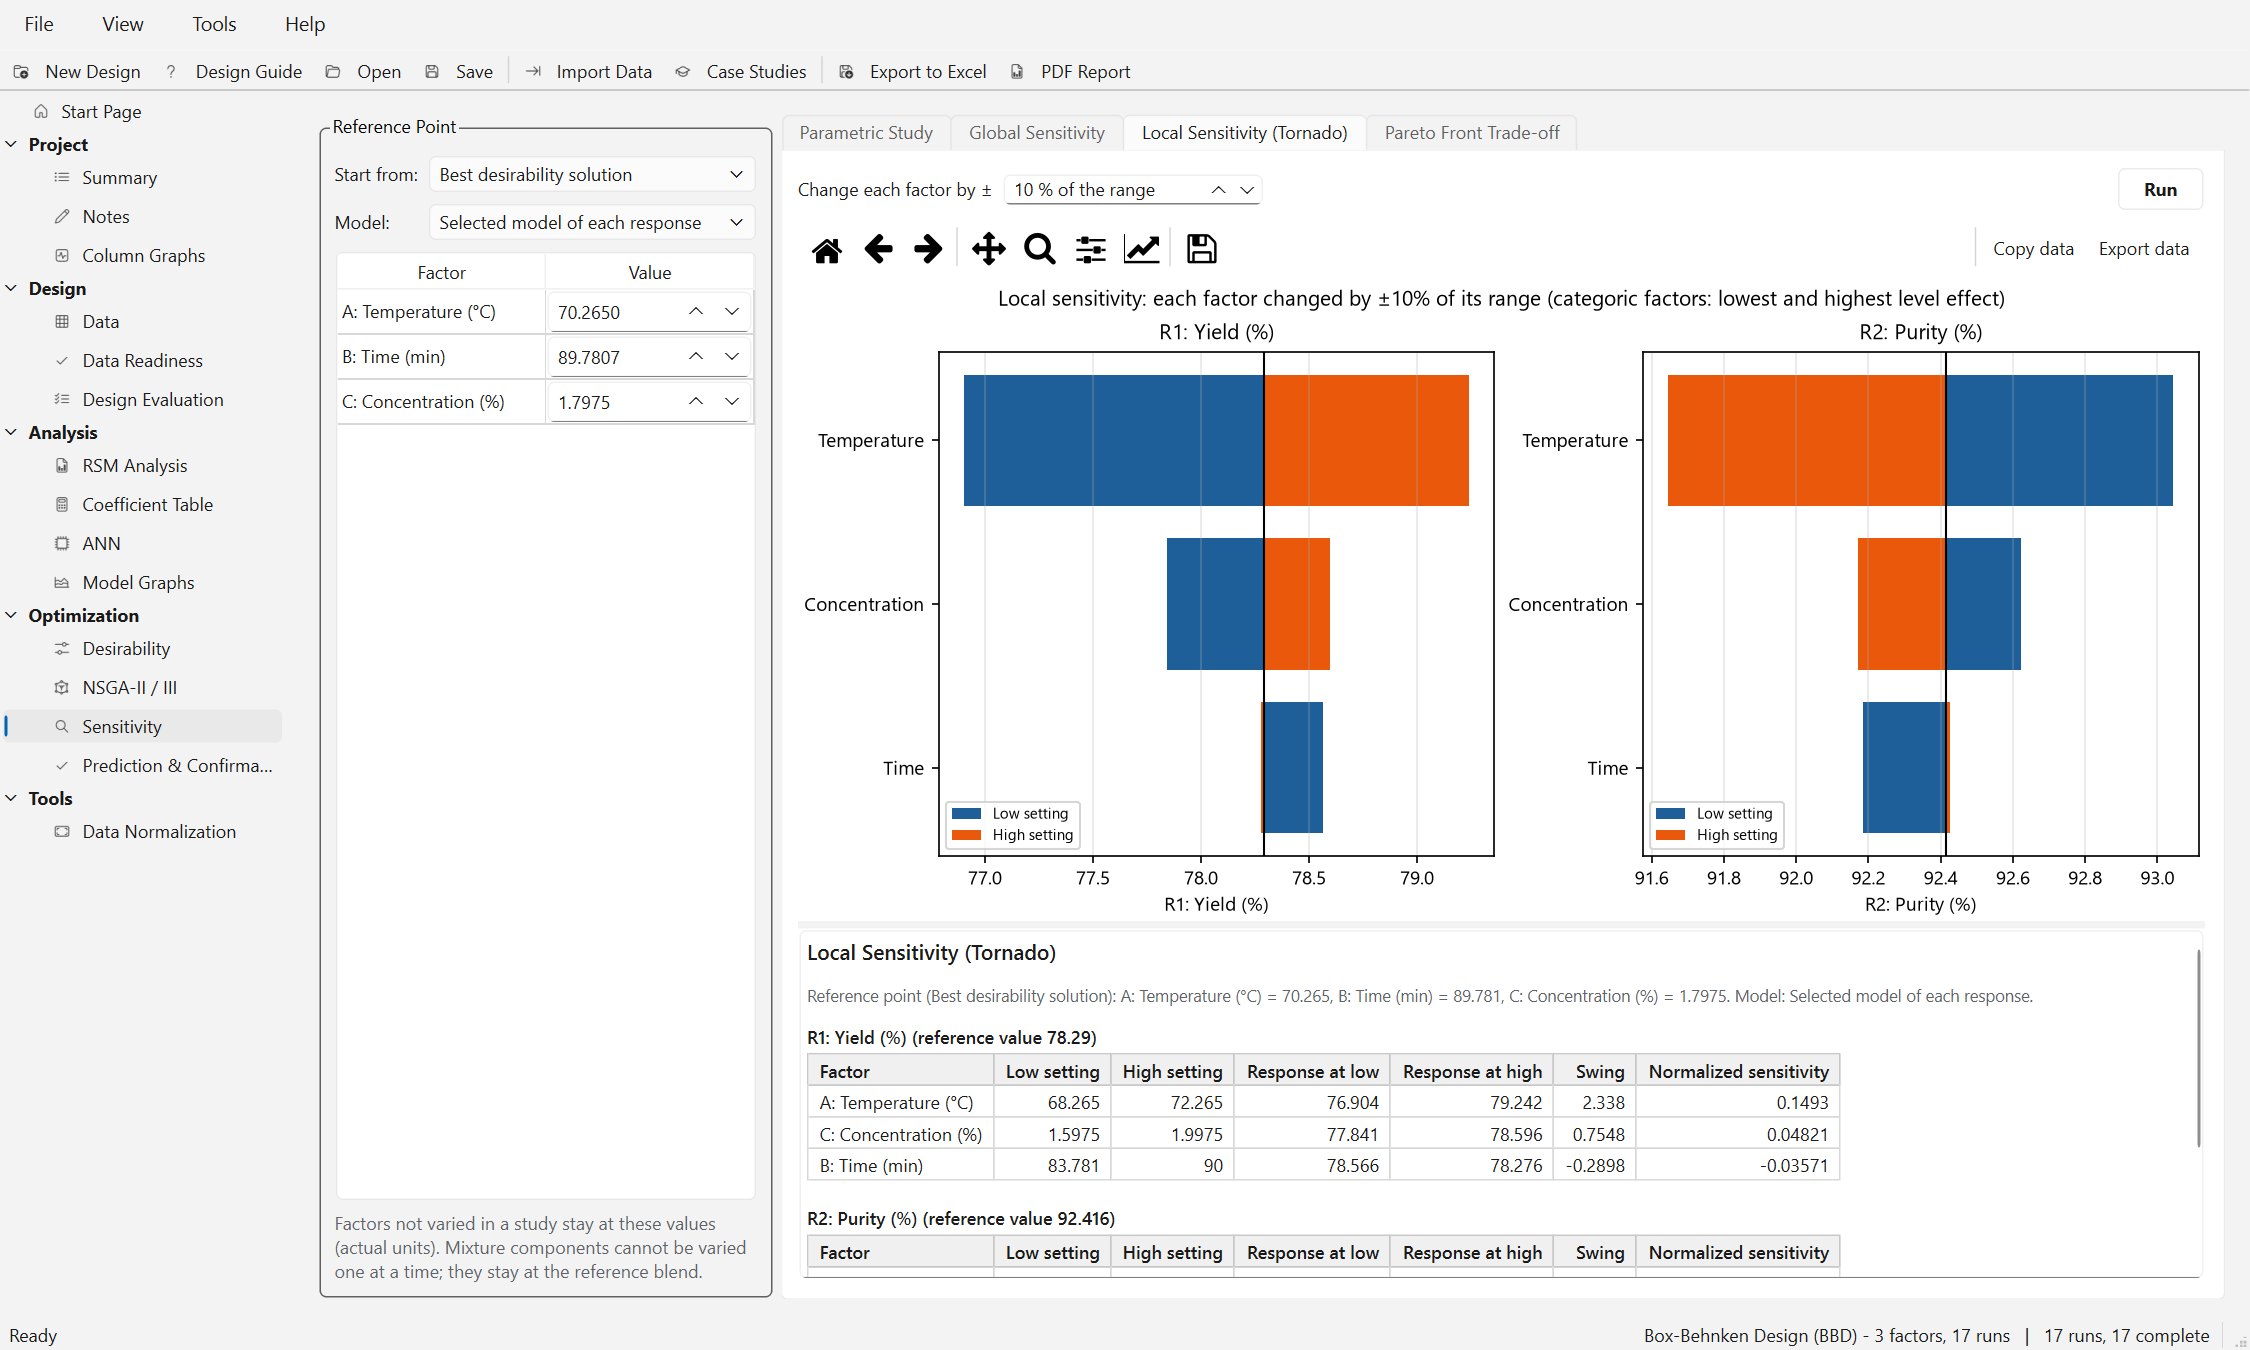
\includegraphics[width=\linewidth]{sens_tornado.png}
\caption{Tornado chart at the best desirability solution, each factor changed by $\pm10$~\% of its range.}
\label{fig:ch09-tornado}
\end{figure}

At the best desirability solution (Figure~\ref{fig:ch09-tornado}): Yield (reference 78.29) changes by 2.338 when
Temperature moves from 68.265 to 72.265~°C ($S^\text{norm}=0.149$), by 0.755 for Concentration 1.5975--1.9975~\%
($0.048$) and by $-0.290$ for Time 83.781--90~min ($-0.036$). The Time step is asymmetric because the reference
(89.78~min) is next to the upper bound. Purity (reference 92.416) changes by $-1.398$ for Temperature ($-0.076$),
$-0.451$ for Concentration and $+0.239$ for Time. Temperature is the factor to control most tightly: a deviation of
$\pm2$~°C moves Yield by more than 1 percentage point in each direction. Time, although globally important (Sobol
$S_T=0.364$ for Yield), hardly matters here because the reference lies near the flat top of the Yield--Time curve.

\textbf{Data export.} As for the other tabs.

% ======================================================================================================
\section{Pareto front trade-off}
\label{sec:ch09-front}

\subsection{Purpose}
The tab \ui{Pareto Front Trade-off} analyzes the last result of the \ui{NSGA-II / III} page (\ui{Uses the last NSGA-II /
NSGA-III result.}): which factors change along the front and thus drive the trade-off, which stay constant and can be
set once, and how strongly the objectives conflict. Without an NSGA result the tab says \ui{Run NSGA-II / NSGA-III on the
multi-objective optimization page first.} Click \ui{Analyze}. The analysis uses the main optimization result, not the
fronts of an ANN versus RSM comparison, and does not depend on the reference point.

\subsection{Theory as implemented}
For each factor that varies on the front and each objective, the Spearman rank correlation \citep{spearman1904}
between the factor values and the objective's response values over the Pareto solutions is computed,
\begin{equation}
\rho=\operatorname{corr}\bigl(\operatorname{rank}(x_i),\operatorname{rank}(y_k)\bigr),
\label{eq:ch09-spearman}
\end{equation}
with its p-value, and likewise between each pair of objectives. A rank correlation is used because the relation along
a front is usually monotonic but not linear. For two objectives, the $n$ solutions are sorted by the first objective
$y_1$ and split into $G=\min\bigl(12,\max(2,\lfloor n/6\rfloor)\bigr)$ groups of neighbouring solutions (about six
solutions per group, at most 12 groups). With $\bar y_{1,g}$ and $\bar y_{2,g}$ the means of group $g$, the trade-off
rate is
\begin{equation}
r_g=\frac{\bar y_{2,g+1}-\bar y_{2,g}}{\bar y_{1,g+1}-\bar y_{1,g}},\qquad g=1,\dots,G-1,
\label{eq:ch09-rate}
\end{equation}
plotted at the midpoint $(\bar y_{1,g}+\bar y_{1,g+1})/2$ (pairs of groups with equal mean $y_1$ give no value).
Averaging over groups avoids the very noisy rates that single neighbours with almost equal objective values would
give.

\subsection{Output and how to read it}
The graph contains a heat map \ui{Factor vs objective on the front} of $\rho$ (red positive, blue negative), one panel
per factor showing its value along the front against the first objective, and, for two objectives, the panel
\ui{Trade-off rate along the front}. The report lists $\rho$ and p for every factor and objective and the correlation
matrix of the objectives.
\begin{itemize}
  \item $|\rho|$ close to 1: the factor changes steadily along the front and drives the trade-off; choosing a point
        on the front means choosing this factor.
  \item $\rho$ close to 0: the factor stays nearly constant on the front; set it once.
  \item A negative correlation between two objectives means they conflict; $\rho=-1$ is a perfect conflict, typical
        of two-objective fronts.
  \item The trade-off rate says how much of the second objective is lost per unit gained in the first, averaged over
        groups of neighbouring solutions (the note under the report says ``computed between the means of groups of
        neighbouring solutions''). Each point therefore describes a stretch of the front, not a single solution;
        read the trend.
  \item The p-values describe the ordering of the solutions on this front, not the uncertainty of the models.
\end{itemize}

\subsection{Example}
\begin{figure}[htbp]
\centering
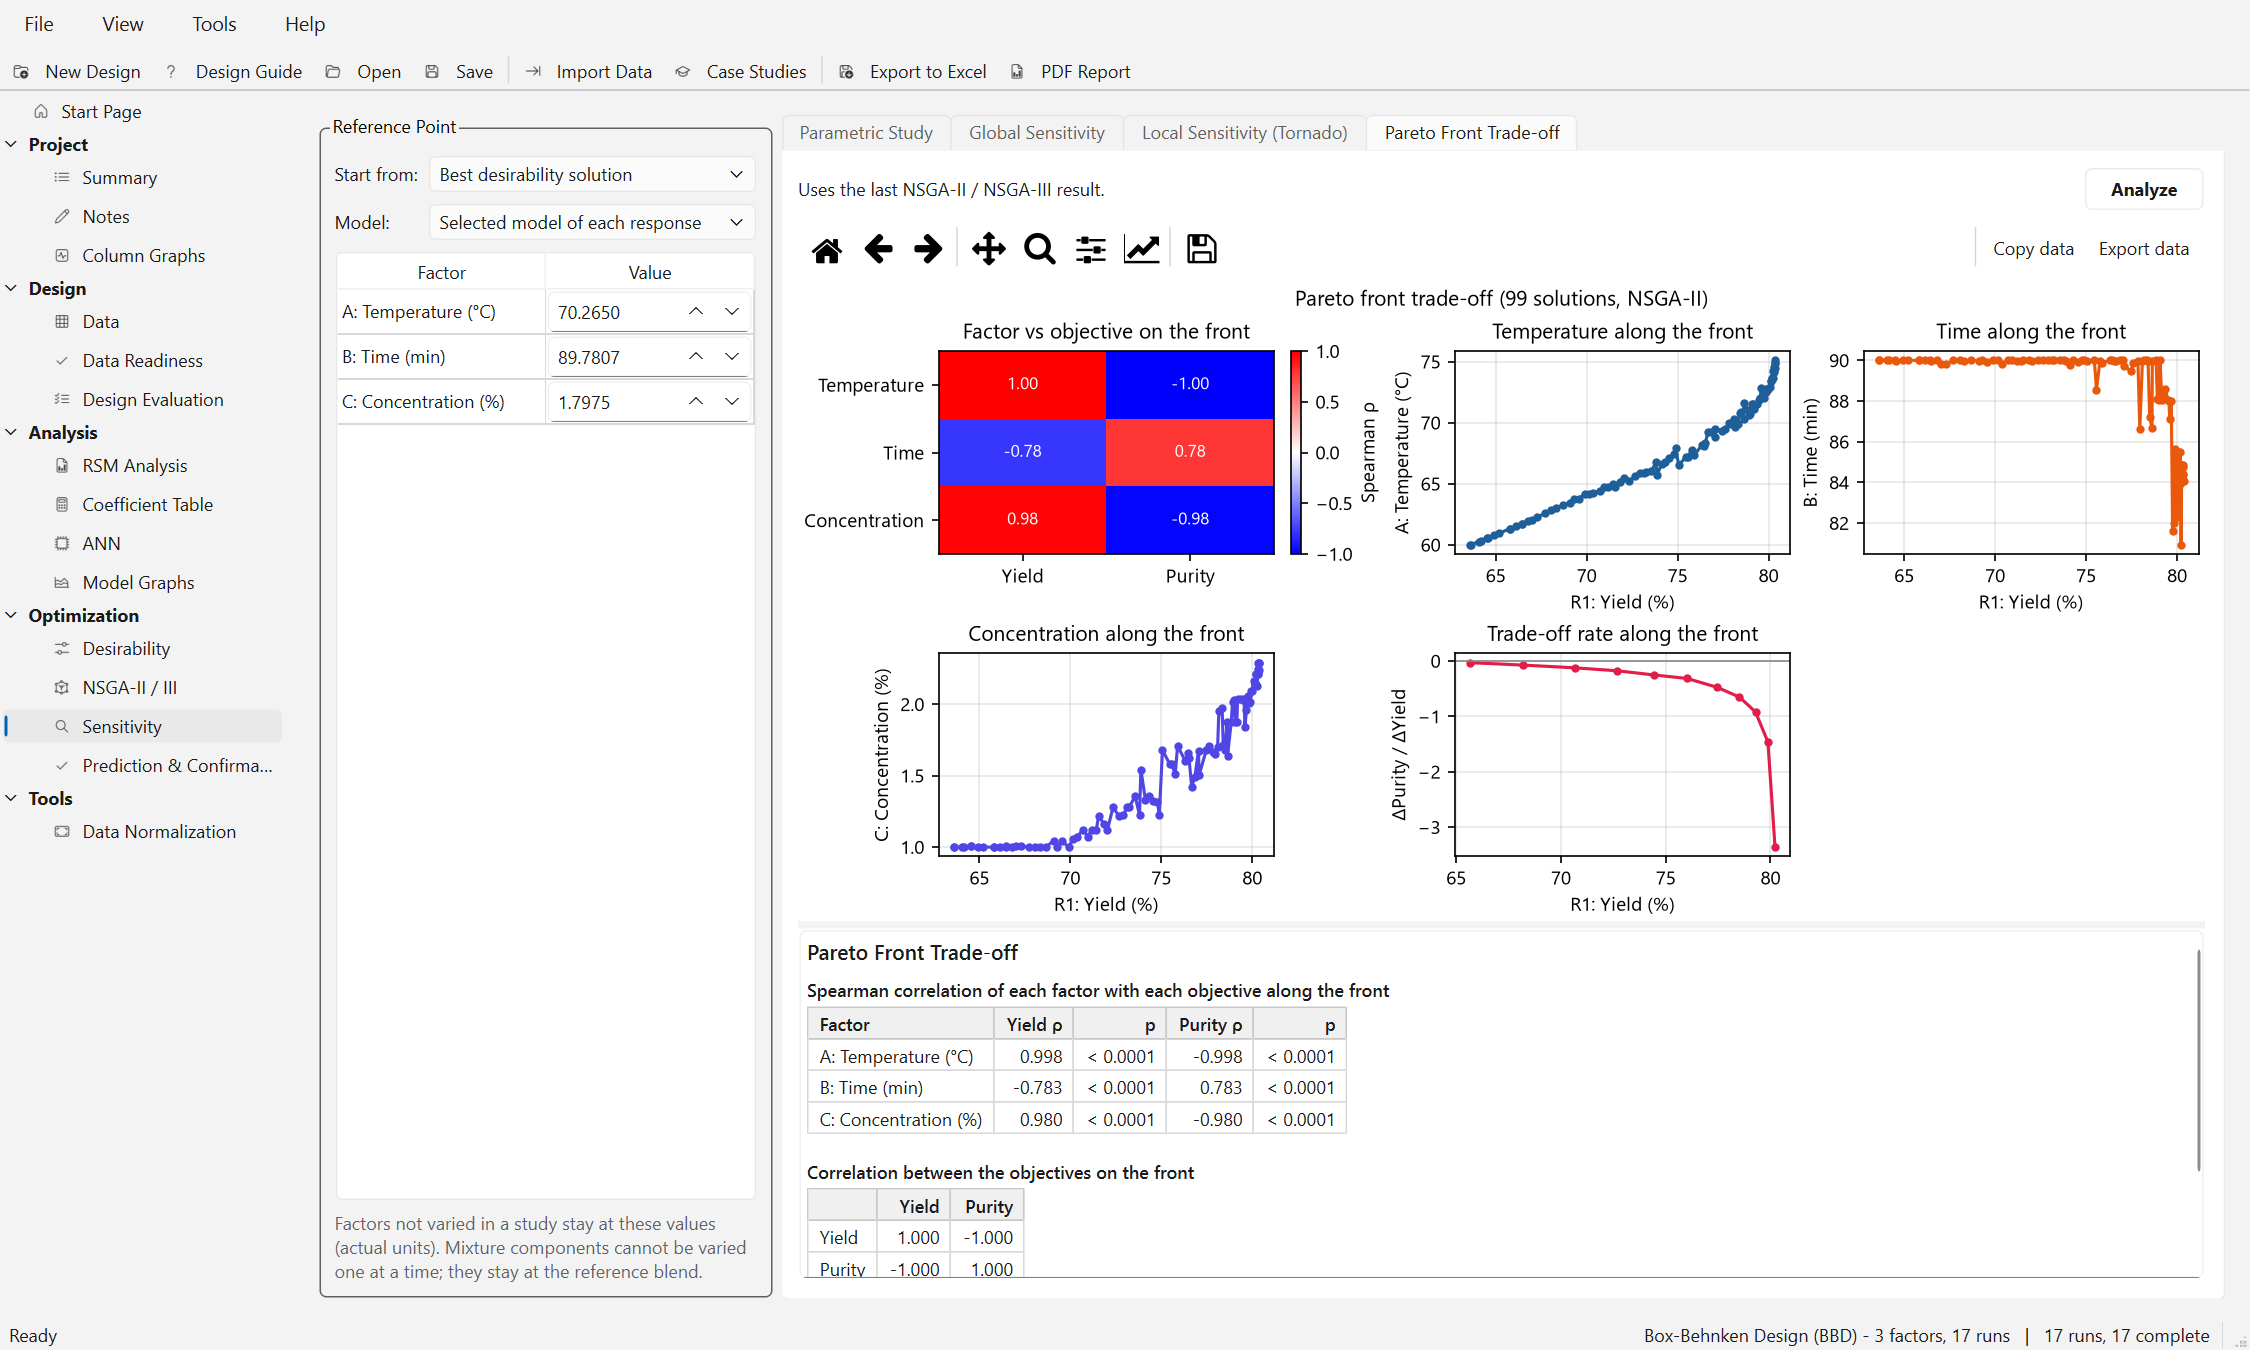
\includegraphics[width=\linewidth]{sens_front.png}
\caption{Pareto front trade-off of the BBD NSGA-II result (title ``Pareto front trade-off (99 solutions,
NSGA-II)''): Spearman heat map, each factor along the front, and the trade-off rate between 12 groups of neighbouring
solutions.}
\label{fig:ch09-front}
\end{figure}

For the BBD front (Figure~\ref{fig:ch09-front}), Temperature ($\rho=+0.998$ with Yield, $-0.998$ with Purity) and
Concentration ($\pm0.980$) increase steadily from the high-Purity end to the high-Yield end; Time is less strongly
related ($\rho=-0.783$ with Yield) because it stays at 90~min over most of the front and drops only at the high-Yield
end. Yield and Purity are perfectly conflicting ($\rho=-1.000$). The 99 solutions form 12 groups, which give 11
values of the trade-off rate $\Delta$Purity/$\Delta$Yield. The rate is small at low Yield ($-0.03$ at Yield 65.7,
$-0.12$ at 70.7, $-0.25$ at 74.4) and becomes strongly negative at the high-Yield end ($-0.48$ at 77.5, $-0.92$ at
79.3, $-1.46$ at 79.9 and $-3.36$ at 80.2): beyond the knee point (Yield 75.8) every additional unit of Yield costs
increasingly more Purity.

% ======================================================================================================
\section{Example: polygeneration plant}
\label{sec:ch09-polygen}
The BBD example has three factors and two responses. The case \ui{Polygeneration Plant (3 Objectives)} (80 simulated
runs of an illustrative plant model, Chapter~\ref{chap:11}) has five decision variables and three objectives, which is
where the sensitivity page becomes indispensable. The models are the quadratic RSM models (predicted $R^2$ 0.992, 0.967
and 0.990), \ui{Model:} is \ui{Selected model of each response}, and the reference point is \ui{NSGA: TOPSIS choice} of the
NSGA-III run with population 200 (Section~\ref{sec:ch11-polygen}): Geothermal Temperature 218.51~°C, Turbine Inlet
Pressure 1401.3~kPa, Pinch Point 10.665~°C, RO Recovery Ratio 0.7499 and Reinjection Temperature 50.589~°C.

\paragraph{Parametric study.} Figure~\ref{fig:ch09-poly-param} shows the layout \ui{All factors, one panel each} with
11 points. Every panel keeps a readable size; when the figure is larger than the window, the plot area scrolls. Each
panel answers the question ``what happens if only this variable moves away
from the compromise?'':
\begin{itemize}
  \item (a) Geothermal Temperature is the main lever of the conflict: from 160 to 220~°C the Exergy Efficiency rises
        from 15.10 to 20.26~\% and the Product Cost falls from 21.22 to 18.12~USD/GJ, but the Environmental Impact rises
        from 2.94 to 3.96~mPts/h.
  \item (b) Turbine Inlet Pressure raises the efficiency up to a flat maximum (20.96~\% at 1900~kPa) and lowers the
        cost, again at the price of a higher impact (3.68 to 4.36~mPts/h from 1000 to 2000~kPa).
  \item (c) A larger Pinch Point lowers the efficiency (21.37 to 19.24~\%) but also the cost (20.67 to
        17.60~USD/GJ) and the impact (4.20 to 3.89~mPts/h): a cheaper, smaller heat exchanger costs efficiency.
  \item (d) The RO Recovery Ratio barely moves the efficiency (19.65 to 20.13~\%), has a cost minimum near 0.59
        (17.94~USD/GJ), and lowers the impact (4.34 to 3.93~mPts/h); the compromise sits at the upper bound 0.75.
  \item (e) A higher Reinjection Temperature is worse for efficiency and cost and only slightly better for the impact
        (from 50 to 90~°C: efficiency 20.19 to 16.52~\%, cost 18.15 to 20.64~USD/GJ, impact 3.94 to 3.64~mPts/h); the
        compromise sits near the lower bound, at 50.6~°C.
\end{itemize}

\begin{figure}[htbp]
\centering
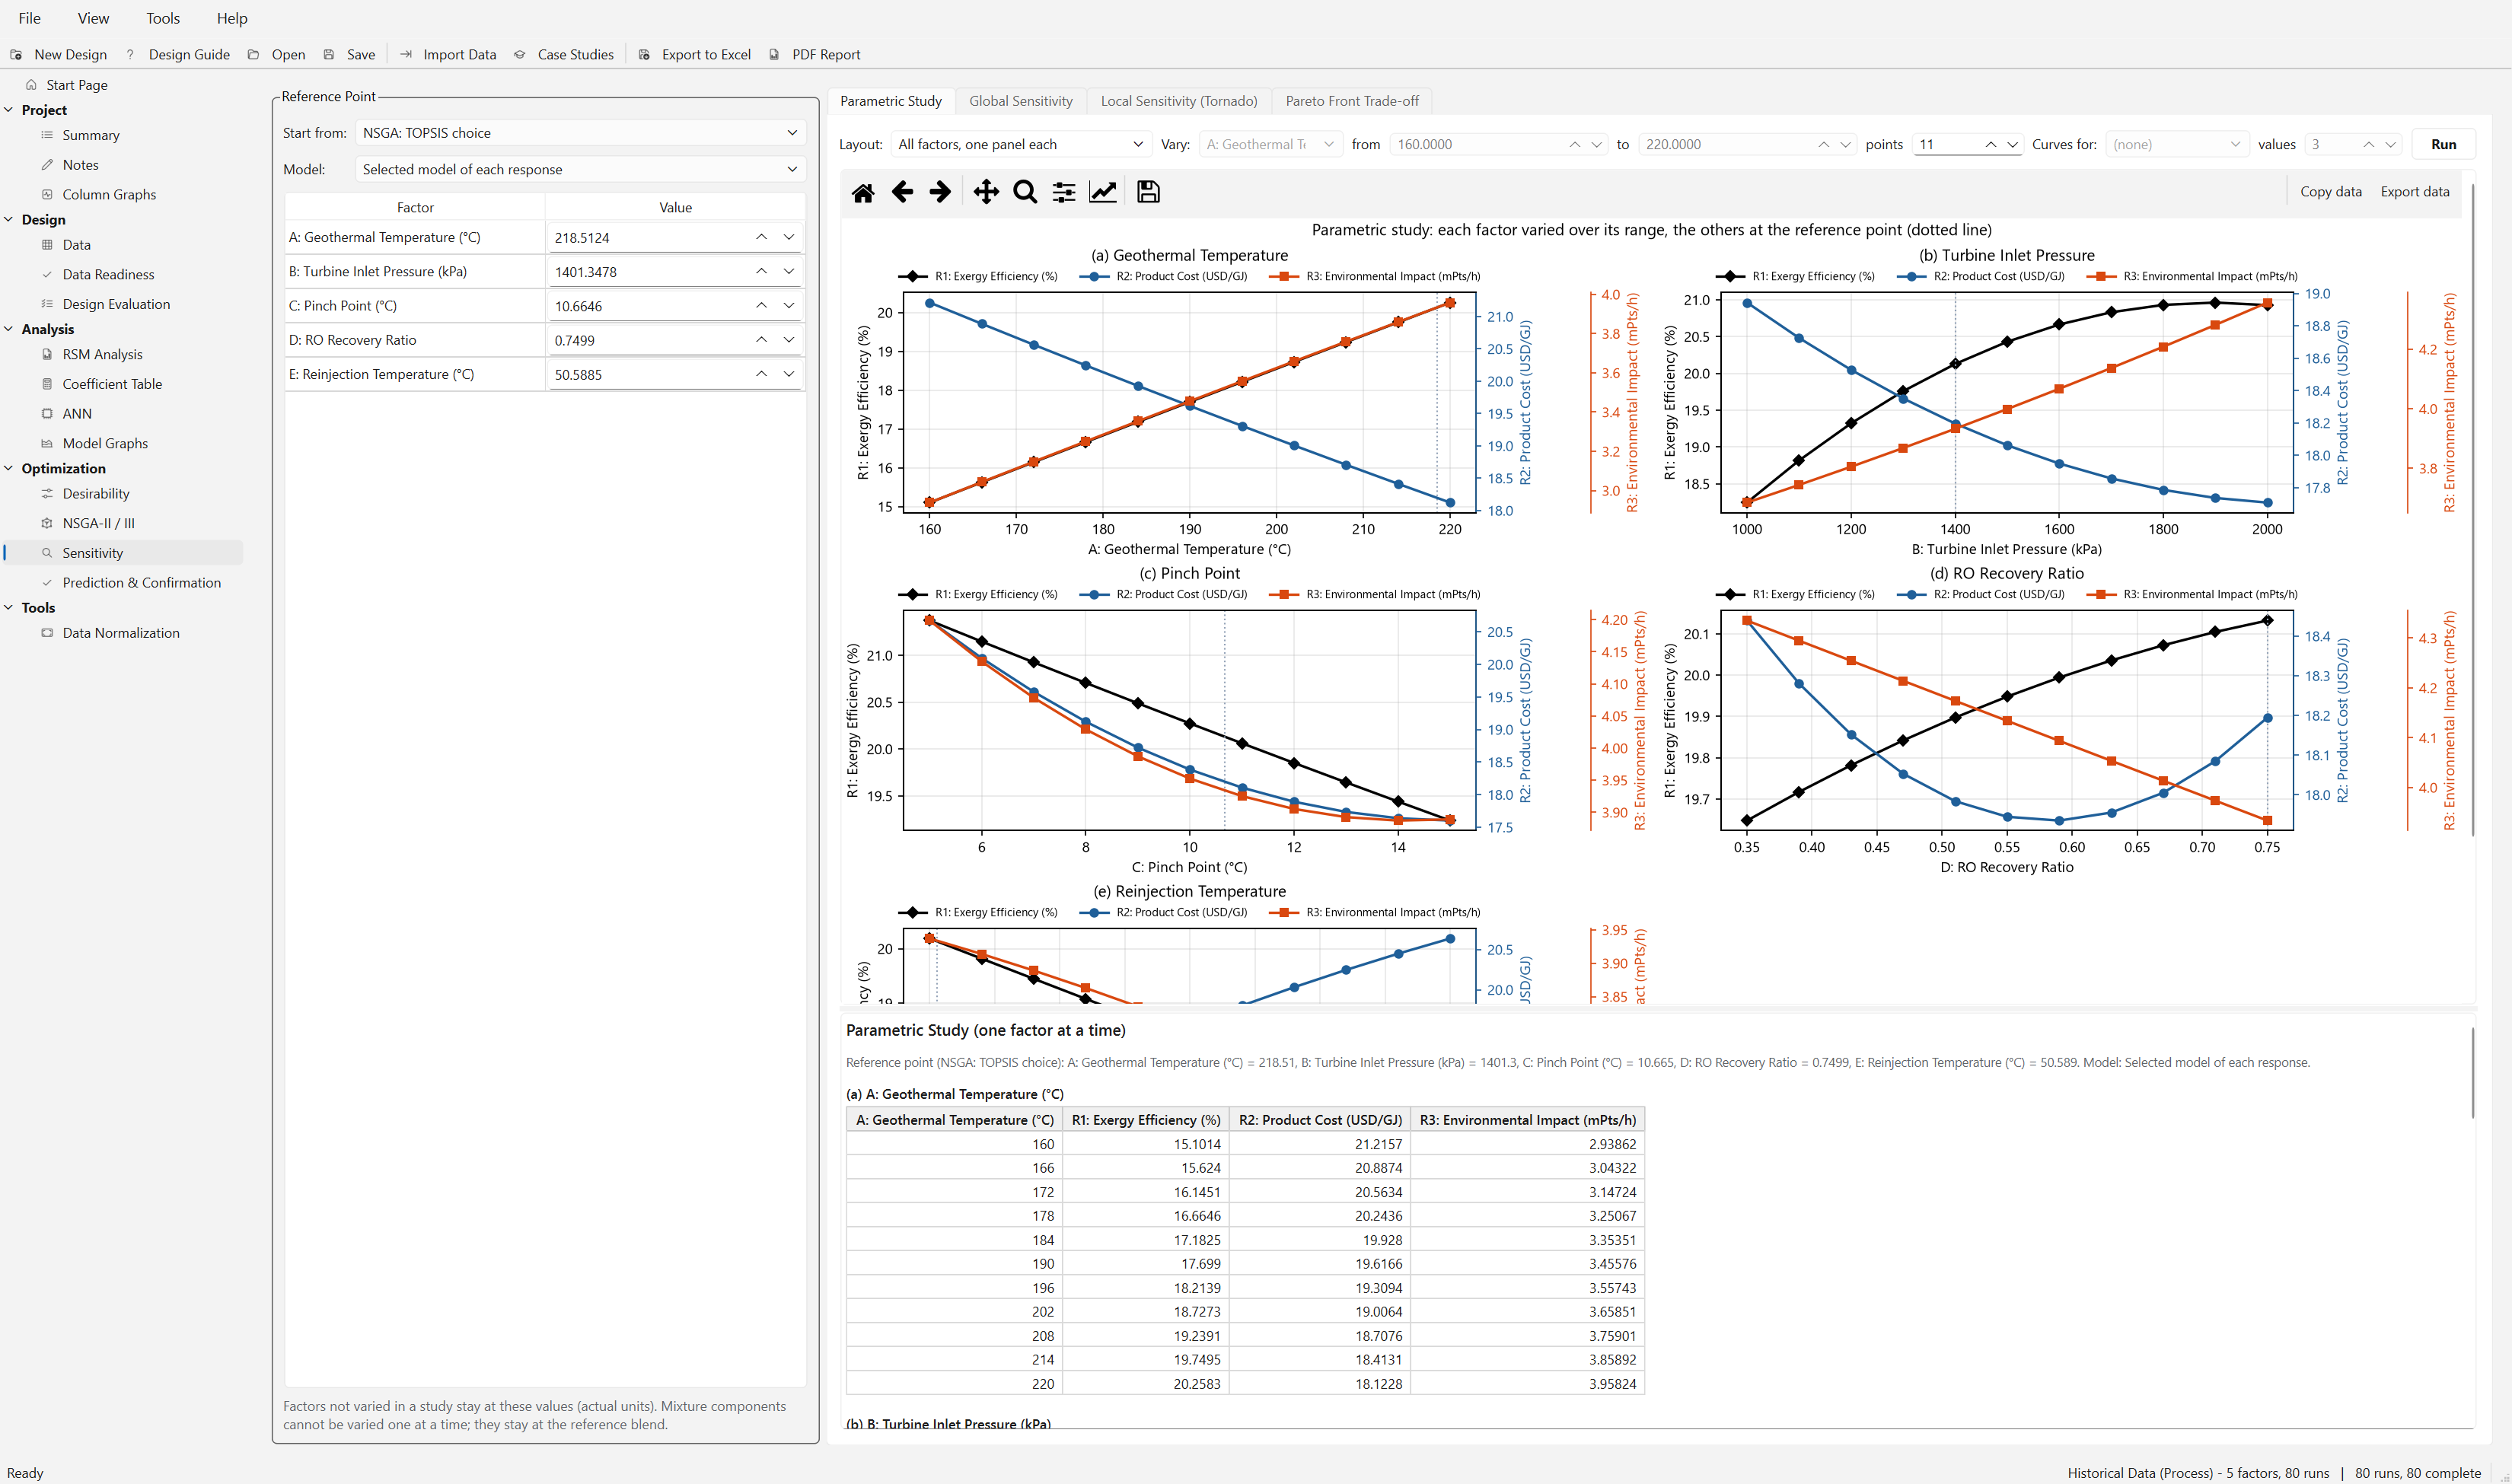
\includegraphics[width=\linewidth]{moo_polygen_parametric.png}
\caption{Parametric study of the polygeneration case from the NSGA TOPSIS choice (\ui{All factors, one panel each}, 11
points). Exergy Efficiency in black (left axis), Product Cost in blue and Environmental Impact in orange
(right axes); the dotted line marks the reference value.}
\label{fig:ch09-poly-param}
\end{figure}

\paragraph{Significance of the decision variables.} The method \ui{Standardized coefficients (Latin hypercube)} with the
default 120 points produces the table \ui{Significance of the Decision Variables} (Figure~\ref{fig:ch09-poly-src},
Table~\ref{tab:ch09-poly-src}). This is the kind of table often reported in thermoeconomic studies: a signed
coefficient per decision variable and objective, with its p-value. The $R^2$ of the linear regression is 0.975, 0.967
and 0.990, so the linear coefficients describe these responses well and $\beta$ can be used to rank the variables.

\begin{table}[htbp]
\centering
\small
\caption{Standardized coefficients $\beta$ (p-value) of the polygeneration case, 120-point Latin hypercube, RSM
models.}
\label{tab:ch09-poly-src}
\footnotesize
\begin{tabular}{@{}llll@{}}
\toprule
Decision variable (range) & Exergy Efficiency & Product Cost & Environmental Impact \\
\midrule
A: Geothermal Temperature (160--220~°C) & $+0.727$ ($<0.0001$) & $-0.582$ ($<0.0001$) & $+0.844$ ($<0.0001$) \\
B: Turbine Inlet Pressure (1000--2000~kPa) & $+0.411$ ($<0.0001$) & $-0.179$ ($<0.0001$) & $+0.497$ ($<0.0001$) \\
C: Pinch Point (5--15~°C) & $-0.363$ ($<0.0001$) & $-0.530$ ($<0.0001$) & $-0.246$ ($<0.0001$) \\
D: RO Recovery Ratio (0.35--0.75) & $+0.077$ ($<0.0001$) & $-0.052$ (0.0036) & $-0.337$ ($<0.0001$) \\
E: Reinjection Temperature (50--90~°C) & $-0.551$ ($<0.0001$) & $+0.427$ ($<0.0001$) & $-0.250$ ($<0.0001$) \\
\midrule
$R^2$ of the linear regression & 0.975 & 0.967 & 0.990 \\
\bottomrule
\end{tabular}
\end{table}

\begin{figure}[htbp]
\centering
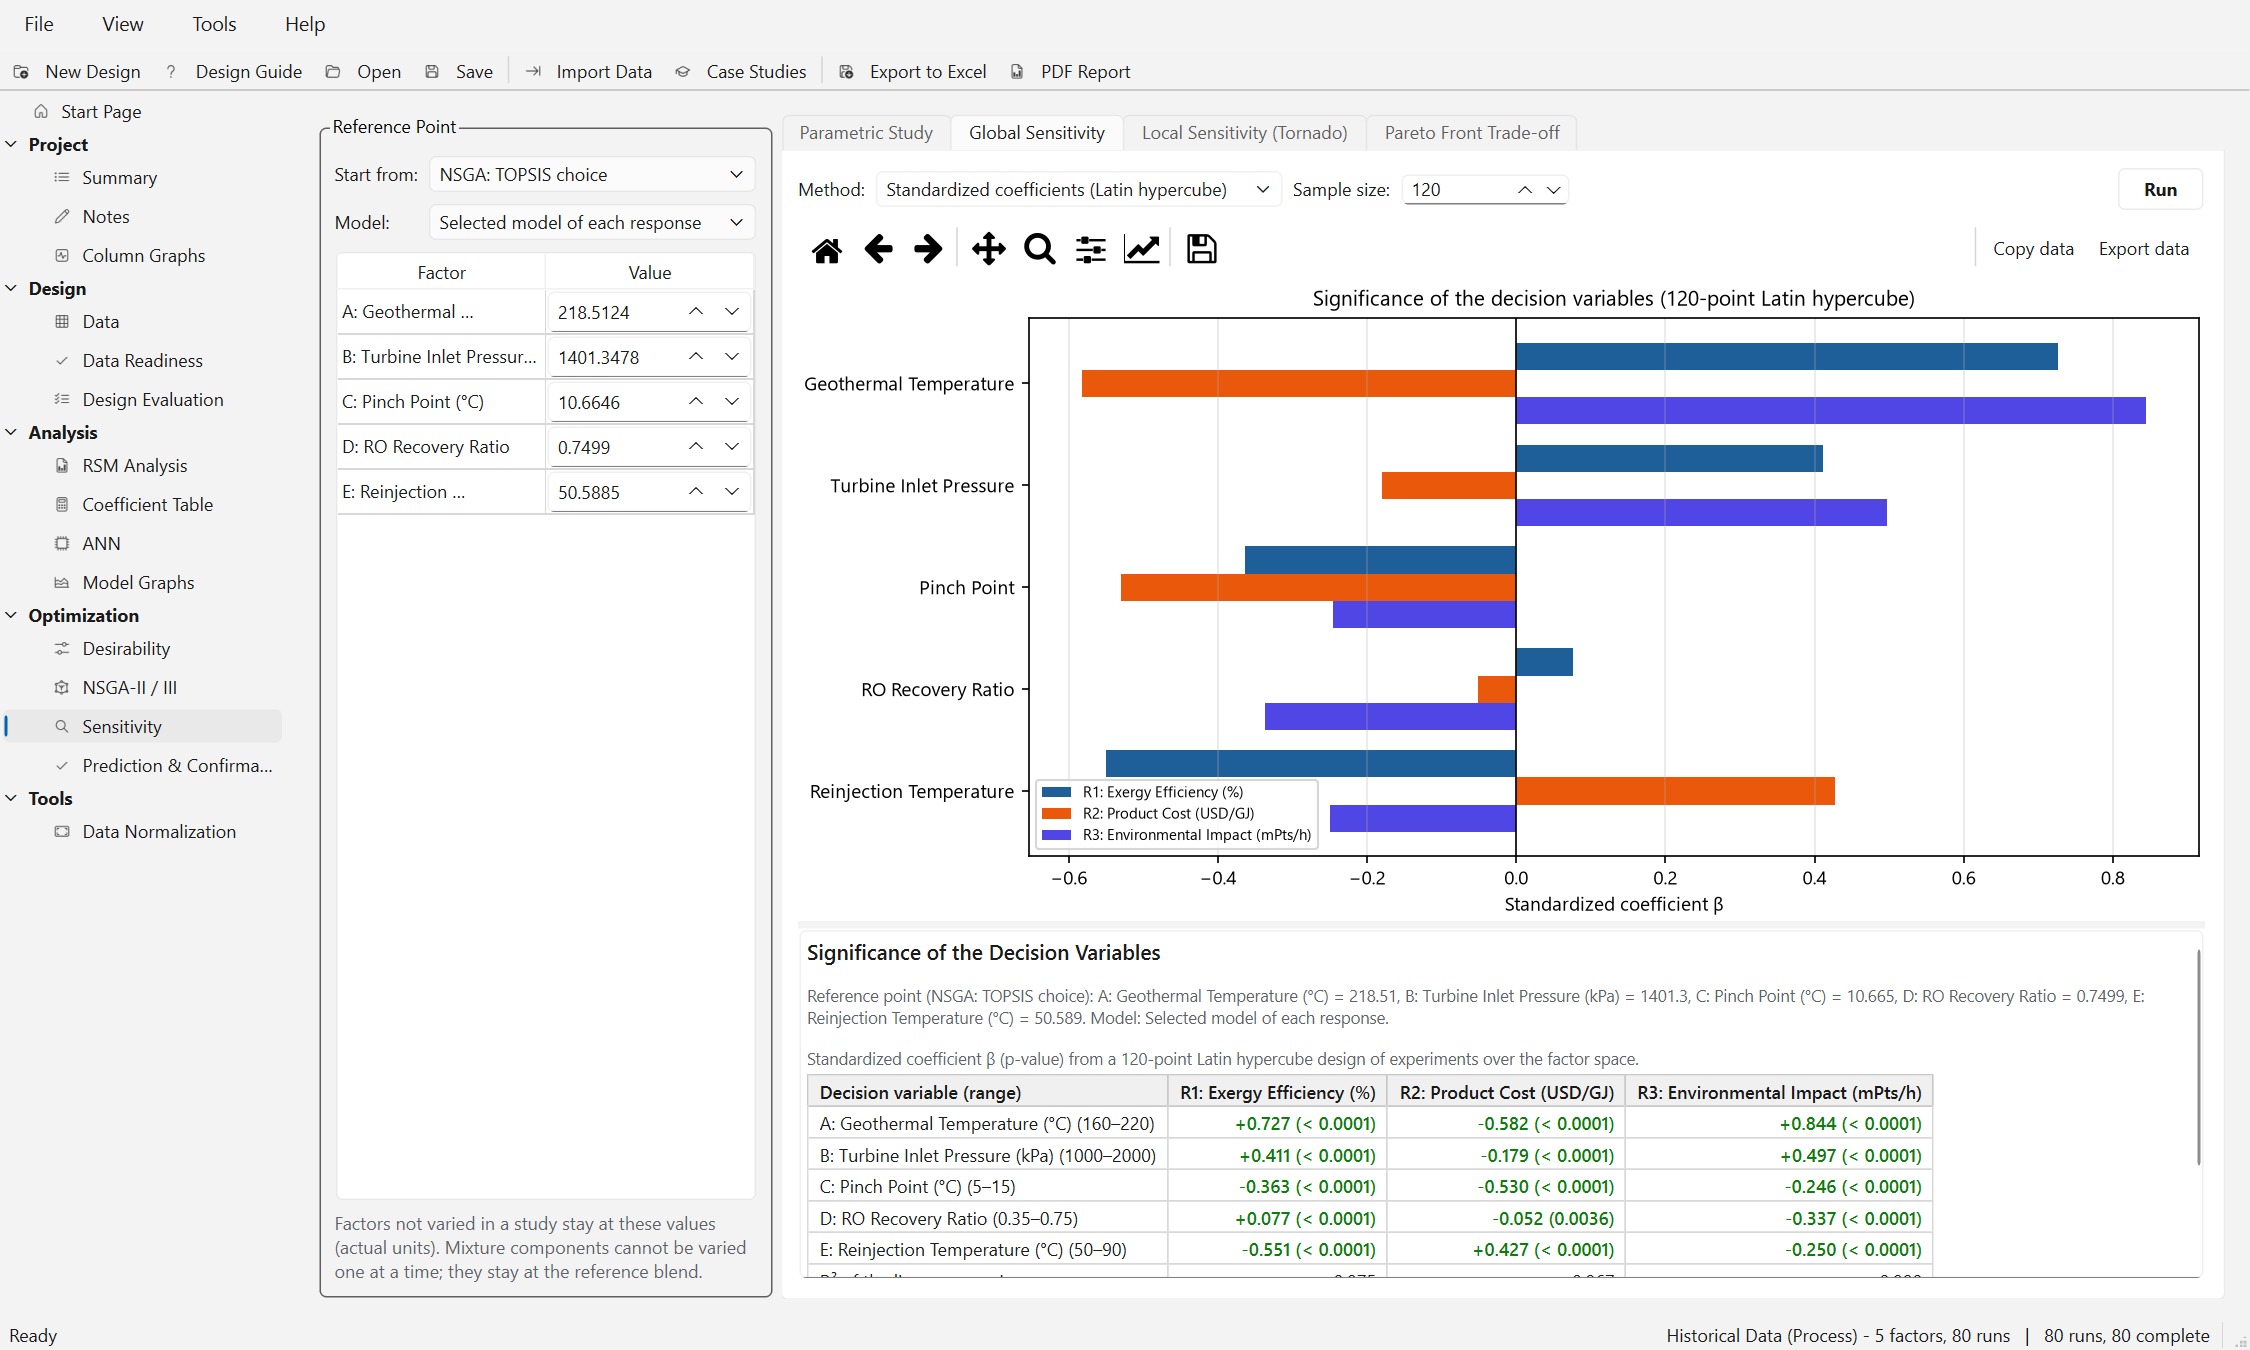
\includegraphics[width=\linewidth]{moo_polygen_src.png}
\caption{\ui{Global Sensitivity}, method \ui{Standardized coefficients (Latin hypercube)}, 120 points: the graph
\ui{Significance of the decision variables} and the table with $\beta$ (p-value) for each objective.}
\label{fig:ch09-poly-src}
\end{figure}

Geothermal Temperature has the largest $|\beta|$ for all three objectives, and its signs (positive for efficiency and
impact, negative for cost) state the conflict in one row: a hotter resource is better for efficiency and cost and
worse for the environment. The Pinch Point is almost as strong a lever for the cost as the temperature ($\beta=-0.530$
against $-0.582$), and the RO Recovery Ratio matters mainly for the impact ($-0.337$). As explained above, every p-value here is small because the sample is
generated from smooth models; the p-values say that the linear trends are clear, not that the plant has been tested.
The one exception is instructive: the RO Recovery Ratio has a small linear effect on cost ($\beta=-0.052$, $p=0.0036$)
because its cost curve has a minimum inside the range (panel (d) above), which a linear coefficient cannot show.

\paragraph{Sobol indices.} The Sobol indices ($N=8192$, 57\,344 model evaluations per response;
Figure~\ref{fig:ch09-poly-sobol}) confirm the ranking and add the share of variance. For Exergy Efficiency:
Geothermal Temperature $S_T=0.465$, Reinjection Temperature 0.258, Turbine Inlet Pressure 0.167, Pinch Point 0.106,
RO Recovery Ratio 0.008. For Product Cost: Pinch Point 0.365, Geothermal Temperature 0.357, Reinjection Temperature
0.221, Turbine Inlet Pressure 0.051, RO Recovery Ratio 0.008. For Environmental Impact: Geothermal Temperature 0.604,
Turbine Inlet Pressure 0.202, RO Recovery Ratio 0.088, Pinch Point 0.057, Reinjection Temperature 0.051. The sums of
$S_1$ are 0.996, 0.998 and 0.998: the responses are almost additive, and $S_T-S_1$ is at most 0.003 for every factor,
so the interactions found significant in the ANOVA (AE for efficiency, AB for impact) are real but small. The RO
Recovery Ratio explains less than 1~\% of the variance of efficiency and cost; for those two objectives it hardly
matters where it is set, but it does matter for the impact (8.8~\%). Note the difference with the parametric study:
the RO Recovery Ratio has a visible cost minimum along one line through the compromise, but over the whole region its
share of the cost variance is small. With more than three factors the factor names under the Sobol graph are rotated;
the table under the graph gives the values.

\begin{figure}[htbp]
\centering
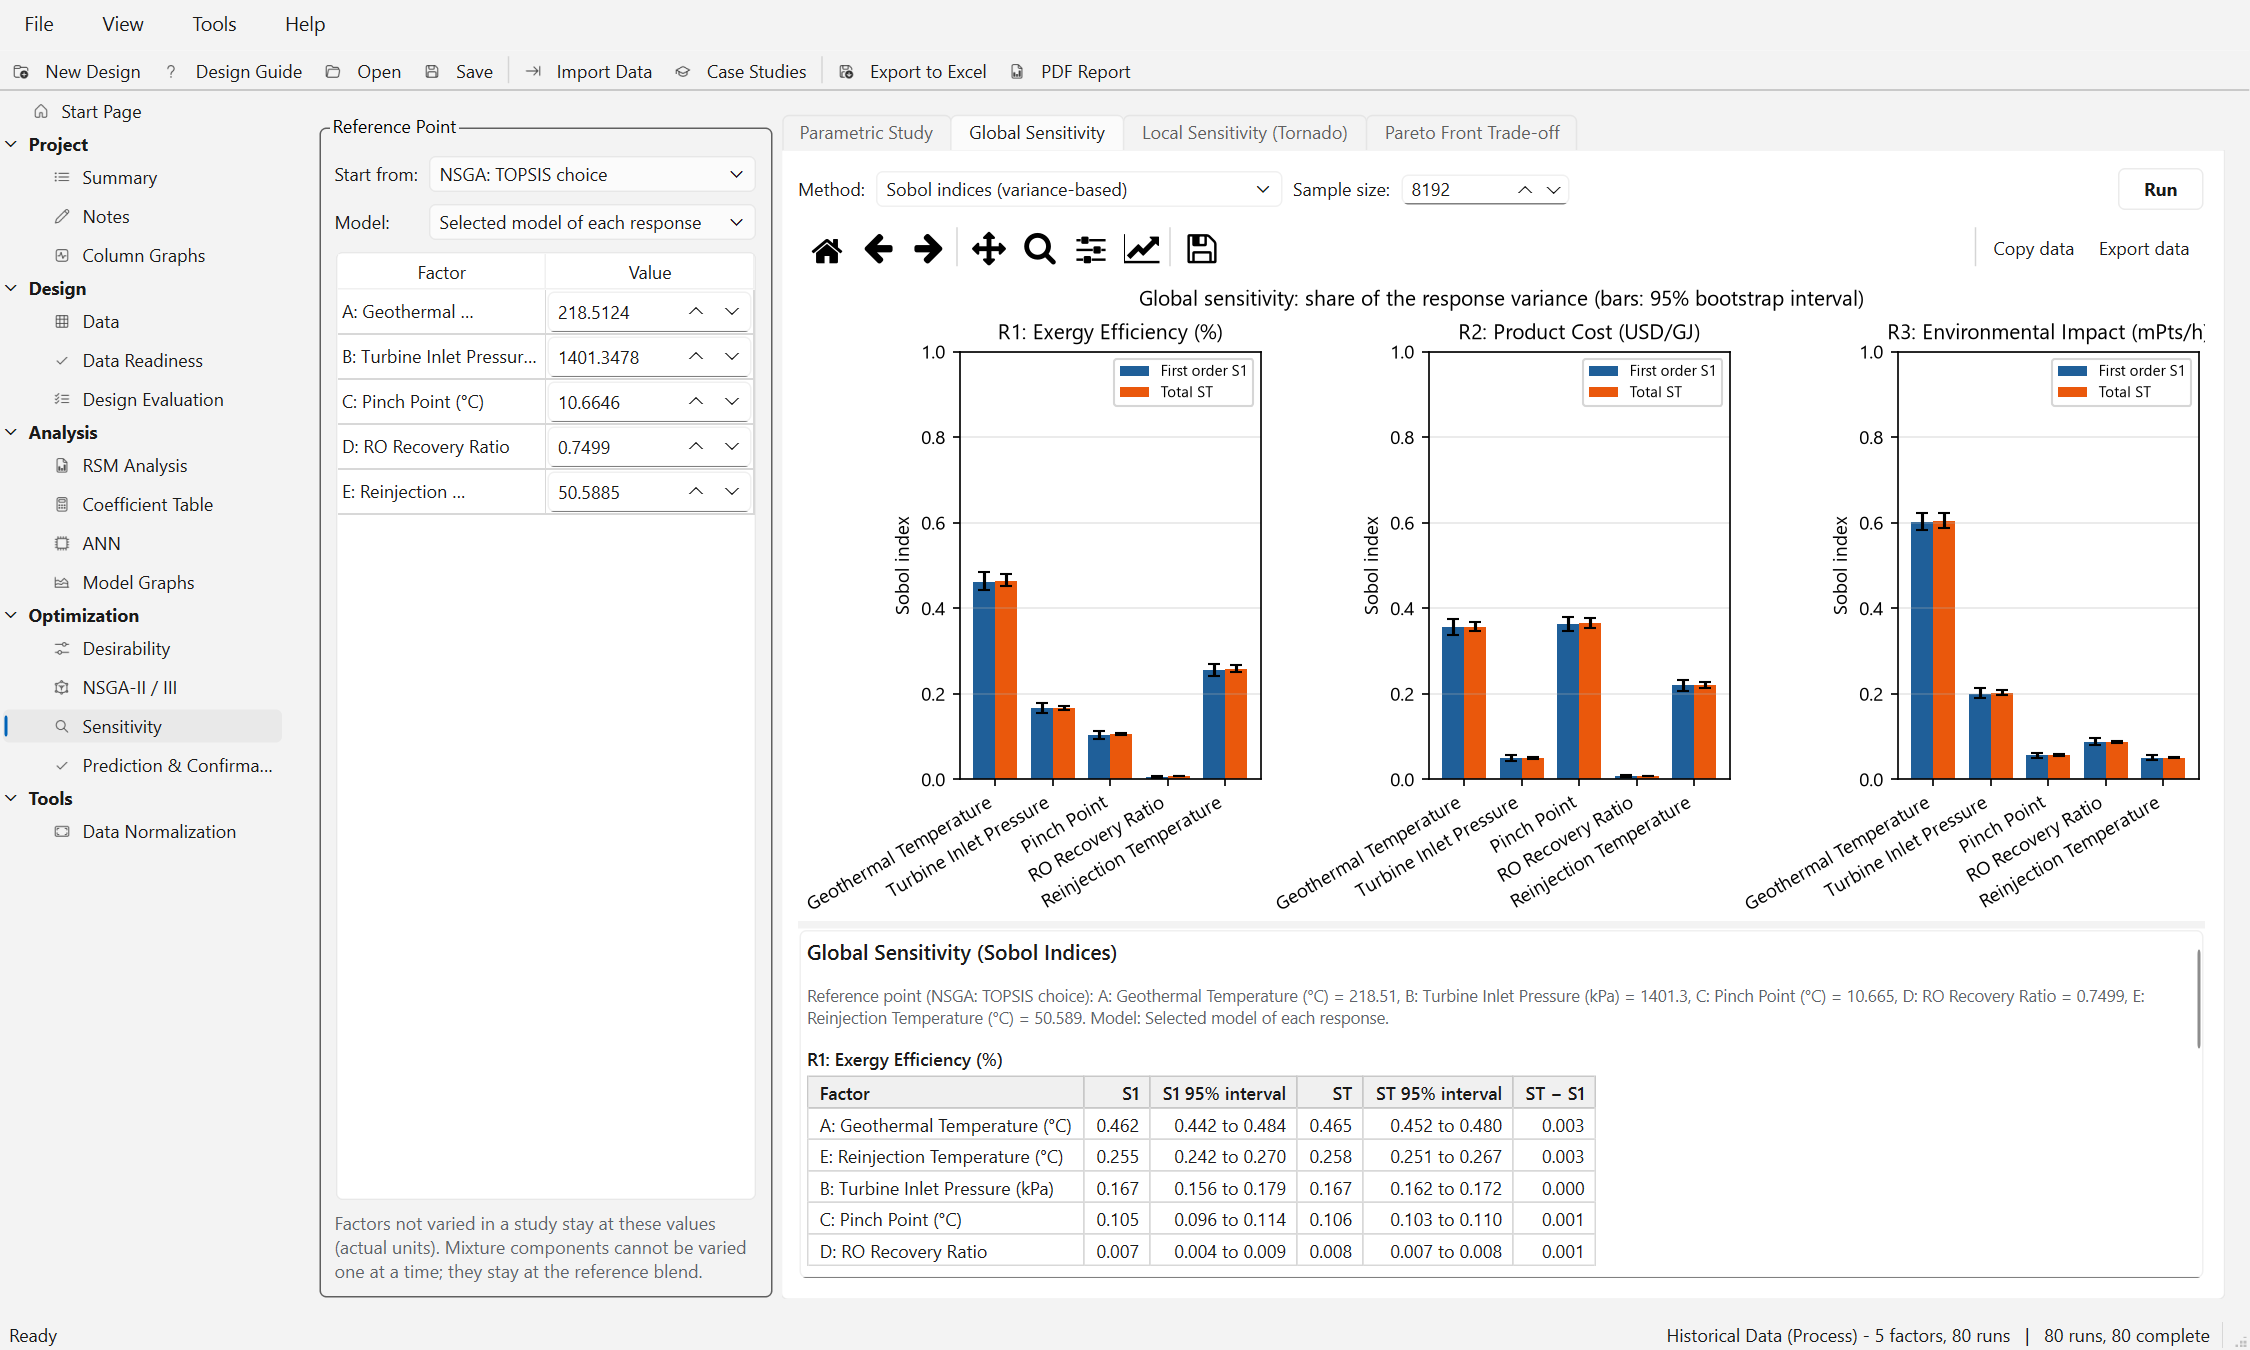
\includegraphics[width=\linewidth]{moo_polygen_sobol.png}
\caption{Sobol indices of the polygeneration case ($N=8192$): first-order $S_1$ and total $S_T$ with 95~\% bootstrap
intervals for each objective.}
\label{fig:ch09-poly-sobol}
\end{figure}

\paragraph{Pareto front trade-off.} The tab \ui{Pareto Front Trade-off} (Figure~\ref{fig:ch09-poly-front}) analyzes the
197 solutions of the NSGA-III front. Geothermal Temperature changes steadily along the front ($\rho=+0.954$ with
Exergy Efficiency, $-0.808$ with Product Cost, $+0.965$ with Environmental Impact): moving along the front essentially
means choosing the resource temperature. Turbine Inlet Pressure follows with $|\rho|$ between 0.38 and 0.56, while the
Pinch Point, the RO Recovery Ratio and the Reinjection Temperature have $|\rho|\le0.38$: the panel of the Reinjection
Temperature shows that it stays at about 50~°C on almost the whole front and rises only at the low-efficiency end. The
correlations between the objectives on the front are $+0.988$ between Exergy Efficiency and Environmental Impact (a
strong conflict, since one is maximized and the other minimized), $-0.711$ between Exergy Efficiency and Product Cost
(both improve together) and $-0.777$ between Product Cost and Environmental Impact (a conflict). The front is
therefore essentially a two-sided trade-off: efficiency and cost on one side, environmental impact on the other, set
mainly by the geothermal temperature. With three objectives the trade-off rate panel is not drawn; it exists only for
two objectives.

\begin{figure}[htbp]
\centering
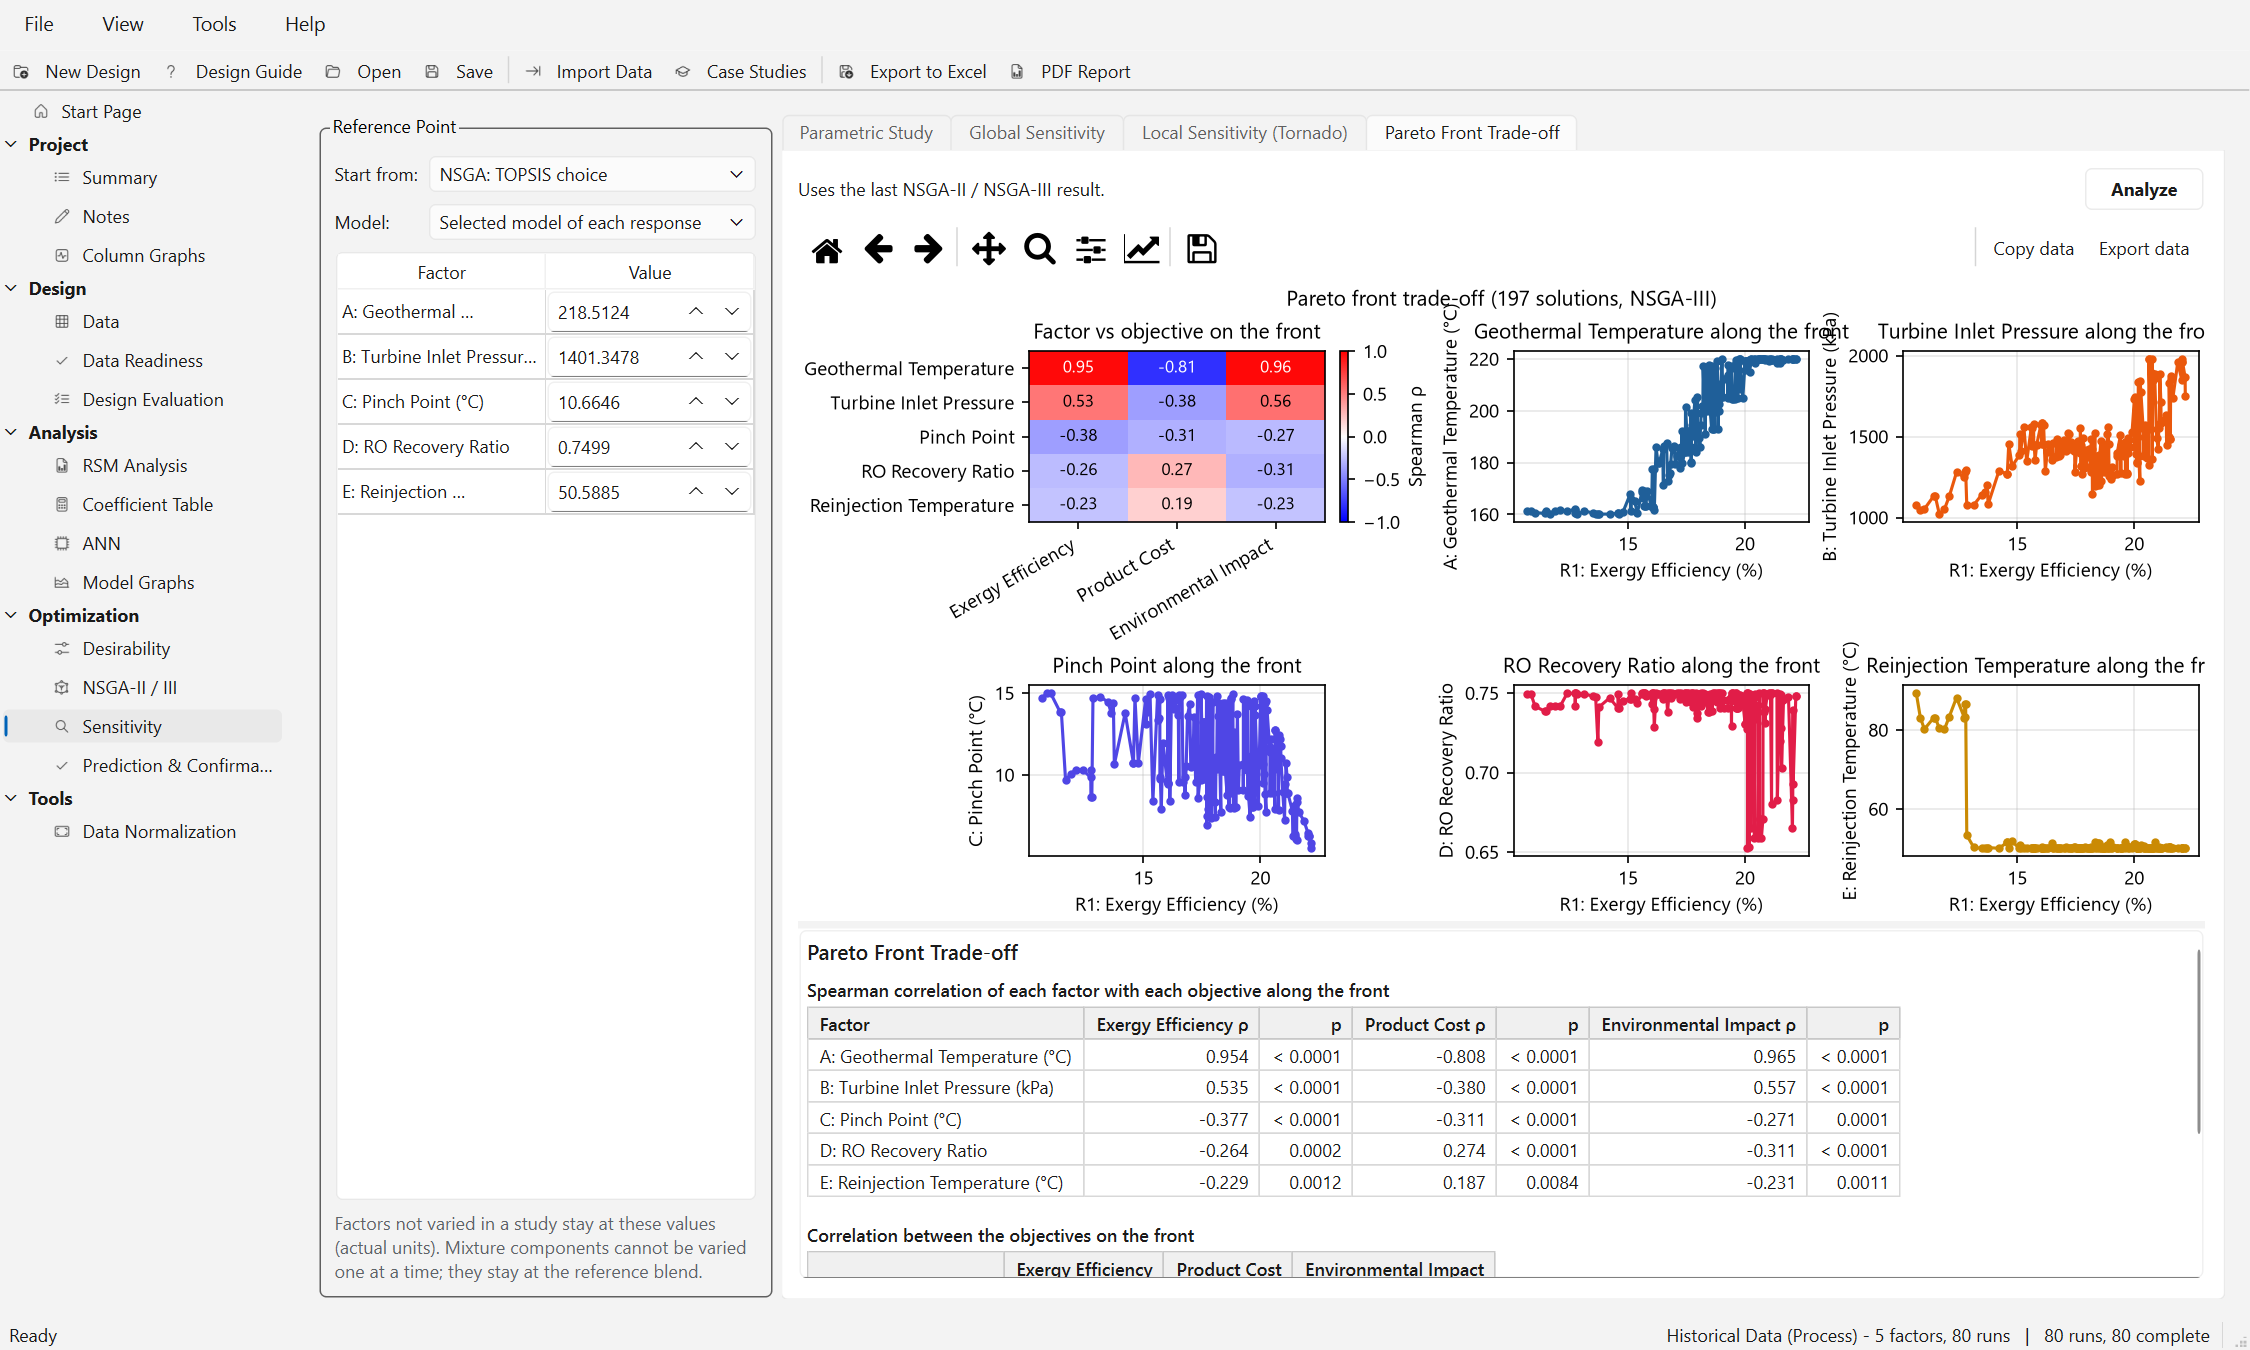
\includegraphics[width=\linewidth]{moo_polygen_tradeoff.png}
\caption{\ui{Pareto Front Trade-off} of the polygeneration NSGA-III front (197 solutions): Spearman heat map and each
decision variable along the front against Exergy Efficiency.}
\label{fig:ch09-poly-front}
\end{figure}

\textbf{Data export.} Each graph has \ui{Copy data} and \ui{Export data\dots}; the significance table, the Sobol tables
and the Spearman tables are exported with \ui{Export all tables\dots} (right-click on the report), ready for a table in
a paper.

% ======================================================================================================
\section{Reporting sensitivity results in a paper}
\label{sec:ch09-reporting}
Sensitivity results are easy to over-interpret. The following practice keeps them honest and reproducible.
\begin{enumerate}
  \item \textbf{Validate the model first.} State the model (RSM order, transform, or ANN architecture) and its
        predictive accuracy (predicted $R^2$, or cross-validated $Q^2$ for an ANN). Sensitivity indices of a poor model
        describe the model, not the process.
  \item \textbf{State the conditions}: the factor ranges, the reference point (for parametric, tornado and any factor
        held fixed), the model, the method and the sample size. The header line of each report contains this
        information.
  \item \textbf{Standardized coefficients}: report $\beta$ with its sign together with the $R^2$ of the linear
        regression. Say that the p-values come from a regression on model predictions and depend on the sample size.
        Do not use them as tests of process effects; use the ANOVA of the fitted model for that.
  \item \textbf{Sobol indices}: report $S_1$ and $S_T$ with their bootstrap intervals, $N$ and the estimators
        (\citealp{saltelli2010} for $S_1$ and \citealp{jansen1999} for $S_T$), the sum of $S_1$, and whether design
        constraints were ignored. Interpret $S_T-S_1$ as interaction.
  \item \textbf{Local sensitivity}: report $\delta$, the reference point and the normalized sensitivity; describe it as
        local.
  \item \textbf{Pareto front}: report the Spearman correlations as a description of the front, together with the
        algorithm, population and the result of check~C.
\end{enumerate}
A sentence for the BBD example could read: ``Variance-based sensitivity analysis of the quadratic models (Sobol indices,
$N=8192$, Saltelli and Jansen estimators, 95~\% bootstrap intervals) showed that temperature explains most of the
variation of both responses over the studied region ($S_T=0.60$ for yield and 0.71 for purity), followed by time for
yield ($S_T=0.36$) and concentration for purity ($S_T=0.15$); interactions account for about 4~\% of the variance
(sum of $S_1=0.96$).''

% Chapter 10: Prediction and Confirmation
\chapter{Prediction and Confirmation}\label{sec:ch10-prediction}\label{chap:10}

An optimization ends with a recommended setting of the factors, but the recommendation is only as good as the model
behind it. The \ui{Prediction \& Confirmation} page (navigation group \ui{Optimization}) answers two questions:
\begin{enumerate}
  \item What does the model predict at a chosen setting, and how precise is that prediction?
  \item After new runs have been made at that setting, do the results agree with the prediction (is the model
    confirmed)?
\end{enumerate}
The examples use the case study \ui{Extraction Optimization (Box-Behnken)} (\menupath{File $\rightarrow$ Case
Studies\dots}): three factors (A: Temperature 60--80~°C, B: Time 30--90~min, C: Concentration 1--3~\%), 17 runs
with 5 center points, and the responses Yield (\%) and Purity (\%), each fitted with the quadratic model on the
\ui{RSM Analysis} page.

\section{The page}\label{sec:ch10-page}

The left side has two groups and a button (Figure~\ref{fig:ch10-prediction}):
\begin{itemize}
  \item \ui{Prediction Point (Actual Units)}: one input per factor, labeled with the factor name and unit. Numeric
    factors use a spin box whose range extends one factor range beyond the design (or data) limits on each side,
    so extrapolation is possible but is flagged. Categorical factors use a list of their levels. For a mixture, a
    line ``Component sum = \dots{} (must be \dots)'' turns red when the components do not add up to the mixture
    total.
  \item \ui{Options}: \ui{Confidence level:} and \ui{Number of confirmation runs (n):}
    (Table~\ref{tab:ch10-options}).
  \item \ui{Reset to Center Point}: sets every numeric factor to the center of its range (coded 0), every
    categorical factor to its first level, and mixture components to the mean of the design. This is also the
    starting point when a project is opened.
\end{itemize}
The right side holds the results table, a warning line in red above it and an explanation below it: CI and PI,
the confirmation rule, the scale of the standard error for transformed and for binomial or Poisson responses, the
note ``Typed confirmation means are cleared when a different point is sent to this page.'' and the confirmation rule
of an ANN. All values are recomputed as soon as an input or an option changes.

\begin{table}[htbp]
\centering
\caption{Options of the \ui{Prediction \& Confirmation} page.}\label{tab:ch10-options}
\begin{tabularx}{\linewidth}{@{}p{4.6cm}p{2.2cm}p{1.4cm}X@{}}
\toprule
Option & Values & Default & Meaning \\
\midrule
\ui{Confidence level:} & 90~\%, 95~\%, 99~\% & 95~\% & Level $1-\alpha$ of the confidence and prediction
  intervals. \\
\ui{Number of confirmation runs (n):} & 1--100 & 3 & Number of new runs whose \emph{mean} will be compared with the
  prediction; sets the width of the prediction interval. \\
\bottomrule
\end{tabularx}
\end{table}

\paragraph{Results table.} One row per response with the columns \ui{Response}, \ui{Prediction}, \ui{Std. Error of
mean}, \ui{CI low}, \ui{CI high}, \ui{PI low}, \ui{PI high}, \ui{Confirmation mean} and \ui{Status}. The response
name ends with ``[ANN]'' when the response is predicted by its neural network (Section~\ref{sec:ch10-ann});
otherwise the model of the \ui{RSM Analysis} page is used. Only \ui{Confirmation mean} can be edited. A dash
(``-'') marks a value that the model cannot provide.

\paragraph{Warnings.} The red line above the table shows any of:
\begin{itemize}
  \item ``The component sum does not equal the mixture total.''
  \item ``This point violates the component bounds / constraints.''
  \item ``The point is outside the design region - the prediction is an extrapolation.'' (process factors: a coded
    value is beyond $\pm1$ and beyond the largest coded value in the data).
\end{itemize}
A prediction with a warning can still be computed, but it should not be trusted without confirmation runs.

\paragraph{Data export.} Right-click the table to copy it (for Excel) or to save it with \ui{Export table\dots}
as an Excel or CSV file.

\section{Predicting at a chosen setting}\label{sec:ch10-predict}

\subsection{How to use}

\begin{enumerate}
  \item Open \ui{Prediction \& Confirmation}.
  \item Type the factor settings in actual units in \ui{Prediction Point (Actual Units)}, or send a solution from
    an optimization page (Section~\ref{sec:ch10-send}).
  \item Choose the confidence level and the number $n$ of confirmation runs you plan to make.
  \item Read the prediction and its intervals in the table.
\end{enumerate}

\subsection{Theory as implemented (RSM)}\label{sec:ch10-theory}

For a least-squares model with model matrix $\mathbf{X}$ ($N$ runs, $p$ coefficients), coefficient estimates
$\mathbf{b}$, residual mean square $\text{MSE}$ and residual degrees of freedom $\nu_\text{E} = N - p$, let
$\mathbf{x}_0$ be the model row of the chosen point (the coded factors expanded into the model terms). Then
\citep{montgomery2017,myers2016}
\begin{align}
  \hat y_0 &= \mathbf{x}_0^\top \mathbf{b}, \qquad
  h_0 = \mathbf{x}_0^\top \left(\mathbf{X}^\top\mathbf{X}\right)^{-1} \mathbf{x}_0, \label{eq:ch10-pred}\\
  \text{SE}_\text{mean} &= \sqrt{\text{MSE}\; h_0}, \qquad
  \text{SE}_{\text{pred},n} = \sqrt{\text{MSE}\left(\frac{1}{n} + h_0\right)}, \label{eq:ch10-se}\\
  \text{CI}:&\quad \hat y_0 \pm t_{1-\alpha/2,\,\nu_\text{E}}\; \text{SE}_\text{mean}, \label{eq:ch10-ci}\\
  \text{PI}:&\quad \hat y_0 \pm t_{1-\alpha/2,\,\nu_\text{E}}\; \text{SE}_{\text{pred},n}. \label{eq:ch10-pi}
\end{align}
The quantity $h_0$ is the scaled prediction variance of the point; it is small near the center of the design and
grows toward its edges and beyond.
\begin{itemize}
  \item The \emph{confidence interval} (CI) covers the true \emph{mean} response at the point. Its width depends only
    on how well the model is estimated there.
  \item The \emph{prediction interval} (PI) covers the \emph{mean of $n$ new runs} at the point. It adds the
    variance $\text{MSE}/n$ of that mean to the uncertainty of the model, so it is always wider than the CI. With
    $n = 1$ it is the usual interval for a single new observation; as $n$ grows it shrinks toward the CI.
\end{itemize}
The interval assumes that the model is correct at the point, that the errors are independent with constant
variance, and that the new runs are made under the same conditions as the experiment. If the model has no residual
degrees of freedom ($\nu_\text{E} = 0$), no intervals can be computed and the cells show ``-''. In a design with
blocks, the prediction is for the average over the blocks (the block effects are set to zero).

\paragraph{Transformed responses.} If a transformation (for example ln or square root) is selected for the
response on the \ui{RSM Analysis} page, the model is fitted to $z = g(y)$. The prediction and the interval limits are
computed on the transformed scale and converted back with $g^{-1}$:
\begin{equation}
  \hat y_0 = g^{-1}(\hat z_0), \qquad
  \left[\min\!\left(g^{-1}(z_\text{lo}), g^{-1}(z_\text{hi})\right),\;
        \max\!\left(g^{-1}(z_\text{lo}), g^{-1}(z_\text{hi})\right)\right].
  \label{eq:ch10-back}
\end{equation}
The back-transformed intervals are therefore not symmetric about the prediction. The column \ui{Std. Error of
mean} is \emph{not} back-transformed: it is the standard error of $\hat z_0$ and is labeled ``(transformed scale)''
(the tooltip of the cell explains this). For an ln transform it is approximately the relative standard error of the
prediction. Note also that the back-transformed prediction estimates the median of the response rather than its
mean when the transformation is nonlinear (for ln, the mean is larger than the median).

\paragraph{Other kinds of models.} For a split-plot design analyzed by REML, the prediction interval of the mean of
$n$ new runs also contains the whole-plot variance: $\text{SE}_{\text{pred},n} = \sqrt{h_0 + \sigma^2_\text{WP} +
\sigma^2/n}$, where $h_0$ is already on the variance scale, and the $t$ quantile uses the residual degrees of
freedom of the split-plot analysis. For a binomial or Poisson response (logistic or Poisson regression), the confidence interval
is a Wald interval on the link scale with a normal quantile, transformed to a proportion or a count; there is no
prediction interval. \ui{Std. Error of mean} is then the standard error of the linear predictor and is labeled
``(link scale, logit)'' or ``(link scale, log)''; its tooltip reads ``Standard error of the linear predictor on the
link scale (logit); the CI is converted back to the response scale.'' (with ``log'' for Poisson).

\subsection{Example: the best desirability solution}

On the \ui{Desirability} page, with Yield and Purity both maximized, the best solution is Temperature 70.265~°C,
Time 89.781~min and Concentration 1.7975~\% (coded $0.027$, $0.993$, $-0.203$). It was sent to the prediction page
with \ui{Send Selected Solution to Prediction}; Figure~\ref{fig:ch10-prediction} shows the result at 95~\% with
$n = 3$.

For Yield, the quadratic model has $p = 10$ coefficients, $\nu_\text{E} = 7$ and $\text{MSE} = 0.5092$; at this
point $h_0 = 0.3633$ and $t_{0.975,7} = 2.3646$. Equations~\eqref{eq:ch10-pred}--\eqref{eq:ch10-pi} give
\begin{align*}
  \hat y_0 &= 78.290, \qquad \text{SE}_\text{mean} = \sqrt{0.5092 \times 0.3633} = 0.4301,\\
  \text{CI} &= 78.290 \pm 2.3646 \times 0.4301 = [77.273,\ 79.307],\\
  \text{SE}_{\text{pred},3} &= \sqrt{0.5092\,(1/3 + 0.3633)} = 0.5956,\\
  \text{PI} &= 78.290 \pm 2.3646 \times 0.5956 = [76.882,\ 79.698].
\end{align*}
For Purity ($\text{MSE} = 0.1385$, same $h_0$ and $t$), the prediction is 92.416 with $\text{SE}_\text{mean} =
0.2243$, CI $[91.886, 92.946]$ and PI $[91.682, 93.151]$.

The leverage $h_0 = 0.363$ is much larger than at the design center ($h_0 = 0.200$) because the optimum lies at the
upper edge of the Time range. At the center the Yield CI is $77.772 \pm 0.755$; at the optimum it is $\pm 1.017$.
Optima often lie at the edge of the design region, where the model is least precise.

\begin{figure}[htbp]
\centering
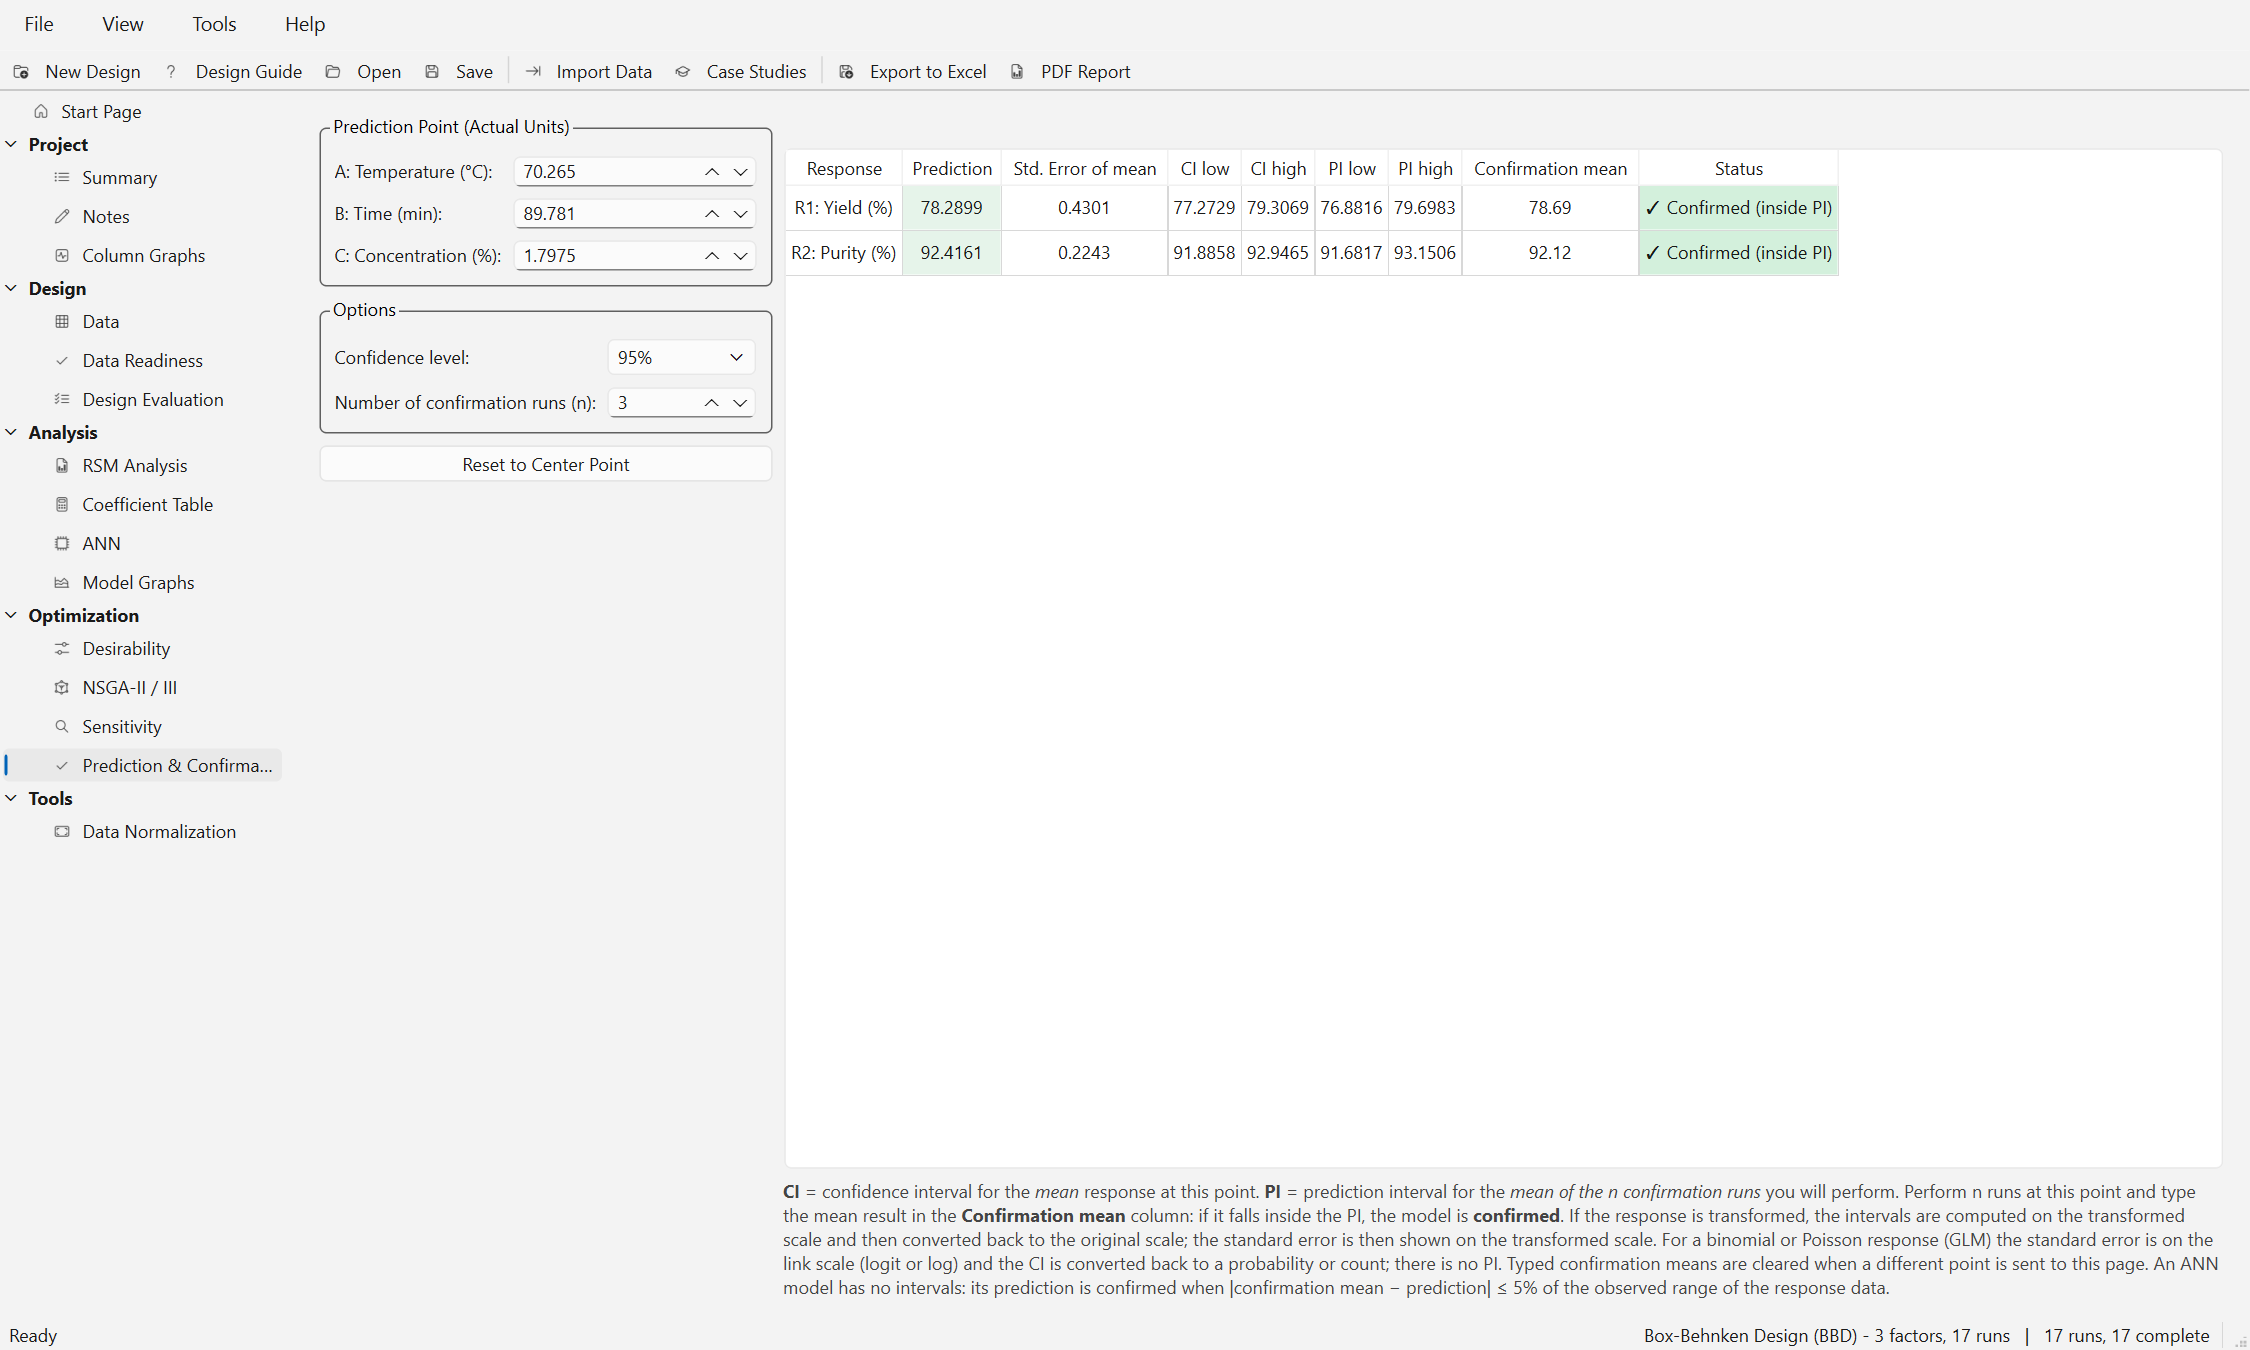
\includegraphics[width=\linewidth]{prediction.png}
\caption{\ui{Prediction \& Confirmation} page with the best desirability solution of the extraction case (95~\%,
$n = 3$). The confirmation means 78.69 (Yield) and 92.12 (Purity) lie inside the prediction intervals: both
responses are confirmed.}
\label{fig:ch10-prediction}
\end{figure}

\section{Predicting with an ANN}\label{sec:ch10-ann}

When the box \ui{Use this response's ANN for graphs, optimization, NSGA-II \& prediction} is ticked on the
\ui{ANN} page (or ANN is chosen in the \ui{Model} column of an optimization page), the response is predicted by its
network and its name ends with ``[ANN]''. The network gives only the point prediction (Eqs.~\eqref{eq:ch07-input}--\eqref{eq:ch07-output} in
Chapter~\ref{chap:7}, with the normalization converted back to response units):
\begin{itemize}
  \item available: \ui{Prediction};
  \item not available (shown as ``-''): \ui{Std. Error of mean}, the CI and the PI. A neural network fitted by
    REGEN has no standard error or interval, because its parameters are not estimated by a linear model with known
    sampling distribution.
\end{itemize}
The uncertainty of an ANN prediction is best judged from the cross-validated test RMSE of the architecture search
(Chapter~\ref{chap:7}): it is the typical error to expect at a new point inside the region covered by the data. For the dye
adsorption network of Chapter~\ref{chap:7} it is 4.07 percentage points of removal efficiency. Outside that region, or in
gaps between the runs, the error can be much larger.

\section{Sending solutions from the optimization pages}\label{sec:ch10-send}

Instead of typing a point, send it from an optimization:
\begin{itemize}
  \item \ui{Desirability}: select a row of the solutions table and click \ui{Send Selected Solution to
    Prediction}.
  \item \ui{NSGA-II / III}: select a Pareto solution and click \ui{Send Selected Solution to Prediction}; without a
    selection the TOPSIS compromise solution is sent.
\end{itemize}
The page opens with the factor inputs set to the solution. Each response is predicted with the model selected for
it (RSM or ANN), as in the optimization. Values typed earlier in \ui{Confirmation mean} belong to the previous point:
they are cleared when a different point is sent to the page (also by \ui{Reset to Center Point} when the point was
not already the center), and kept when the same point is sent again. (When you
change the factor inputs by hand, the typed values stay and are judged against the new prediction; clear them
yourself in that case.)

\section{Confirmation runs}\label{sec:ch10-confirm}

\subsection{How to use}

\begin{enumerate}
  \item Choose the point and set \ui{Number of confirmation runs (n):} to the number of runs you will make.
  \item Make the $n$ runs at the point (Section~\ref{sec:ch10-advice}) and compute the mean result of each response.
  \item Type the mean in the \ui{Confirmation mean} column of each response. A decimal point or a decimal comma may
    be used.
  \item Read the \ui{Status} column.
\end{enumerate}
Confirmation values are kept while the project is open but are not saved in the project file. Record them in the
\ui{Notes} page or in the data table if they should be kept.

\subsection{Confirmation rules}

\paragraph{RSM model.} The model is confirmed when the mean of the $n$ runs falls inside the prediction interval
for the mean of $n$ runs, Eq.~\eqref{eq:ch10-pi}:
\begin{equation}
  \text{PI}_\text{low} \le \bar y_\text{conf} \le \text{PI}_\text{high}. \label{eq:ch10-rule-rsm}
\end{equation}
The status is ``\checkmark{} Confirmed (inside PI)'' on a green background or ``$\times$ Outside PI'' on a red one.
For binomial and Poisson responses only the CI exists, and the statuses are ``Confirmed (inside CI)'' and ``Outside
CI''. A value that cannot be read gives ``Not a number''.

At the confidence level $1-\alpha$, a correct model gives a confirmation mean outside the PI with probability
$\alpha$ (5~\% at the default level). A single result outside the PI is therefore evidence, not proof, that the model
is wrong at this point, and a result inside it does not prove the model correct elsewhere.

\paragraph{ANN model.} Because a network has no prediction interval, its prediction is confirmed when the
difference is small compared with the spread of the response in the data:
\begin{equation}
  \left|\bar y_\text{conf} - \hat y_0\right| \le 0.05\,\left(y_\text{max} - y_\text{min}\right),
  \label{eq:ch10-rule-ann}
\end{equation}
where $y_\text{max}$ and $y_\text{min}$ are the largest and smallest values of the response among the runs used for
modeling. The status reads, for example, ``\checkmark{} Error 1.676 = 3.01\% of the data range ($\le$ 5\%)''
or ``$\times$ Error \dots{} (> 5\%)''. (If all response values are equal, the relative error $|\bar y_\text{conf} -
\hat y_0|/|\hat y_0|$ is used instead with the same 5~\% limit.)

This rule is an engineering tolerance, not a statistical test. It ignores the number of runs and the noise of the
measurement. If the pure-error standard deviation is large compared with 5~\% of the range, even a perfect model
will often fail it with $n = 1$; if the range is very wide, it is lenient. Compare the tolerance with the noise
before relying on it: in the extraction case, 5~\% of the Yield range (64.13 to 78.29) is 0.71, about twice the
pure-error standard deviation of 0.34, so a mean of three runs (standard error $0.34/\sqrt3 = 0.20$) is a fair test.

\paragraph{Example (RSM).} In Figure~\ref{fig:ch10-prediction}, the means of three confirmation runs are 78.69 for
Yield and 92.12 for Purity. Both lie inside their PIs, $[76.88, 79.70]$ and $[91.68, 93.15]$, so both responses are
confirmed. A Yield mean of 80 would be outside the PI and shown as ``Outside PI''.

\paragraph{Example (ANN).} For the dye adsorption case with the 4-3-1 network of Chapter~\ref{chap:7} selected, the
prediction at the center of the factor space (pH 6, Adsorbent Dose 2.25~g/L, Contact Time 65~min, Initial
Concentration 110~mg/L) is 40.82~\%. The response range in the data is $58.45 - 2.73 = 55.72$, so the tolerance is
$0.05 \times 55.72 = 2.79$: a confirmation mean between 38.04 and 43.61 confirms the network. A mean of 42.5 gives
an error of 1.676, which is 3.01~\% of the range, and is accepted.

\subsection{What to do when a confirmation fails}

\begin{enumerate}
  \item Check the runs: were the factor settings, the measurement and the material the same as in the experiment?
    A drift in raw material or equipment shifts all new results.
  \item Check whether the point was an extrapolation or lay in a sparse part of the factor space (warning line,
    \ui{Data Readiness} page, ANN data adequacy).
  \item Add the confirmation runs to the data as ordinary runs and refit the model. Several confirmation points
    around the optimum also improve the model where it matters most (the \ui{Data Readiness} page can suggest them).
  \item If the model is systematically wrong (lack of fit on the \ui{RSM Analysis} page), consider a higher-order
    model, a transformation or an ANN; if the ANN fails, consider RSM or more runs (learning curve, Chapter~\ref{chap:7}).
  \item Repeat the optimization with the refitted model and confirm again.
\end{enumerate}

\section{Planning confirmation runs}\label{sec:ch10-advice}

\paragraph{Number of runs.} The prediction interval narrows as $n$ grows, but never below the confidence interval.
For Yield at the desirability solution (95~\%):

\begin{table}[htbp]
\centering
\caption{Prediction interval for the mean of $n$ confirmation runs, Yield at the best desirability solution.}
\label{tab:ch10-n}
\begin{tabular}{@{}lccc@{}}
\toprule
$n$ & $\text{SE}_{\text{pred},n}$ & PI & Half width \\
\midrule
1 & 0.833 & $[76.32,\ 80.26]$ & 1.97 \\
3 & 0.596 & $[76.88,\ 79.70]$ & 1.41 \\
5 & 0.536 & $[77.02,\ 79.56]$ & 1.27 \\
$\infty$ (CI) & 0.430 & $[77.27,\ 79.31]$ & 1.02 \\
\bottomrule
\end{tabular}
\end{table}

Going from one to three runs narrows the interval by 28~\%; going further gains little, because the uncertainty of
the model itself ($h_0$) then dominates. Three to five runs are usually a good compromise. Set
\ui{Number of confirmation runs (n):} to the number you actually make: the interval is valid only for the mean of
that many runs.

\paragraph{How to make the runs.} Confirmation runs must be genuine replicates: set the factors anew for each run,
run them in random order and, if possible, spread them over time, exactly as in the original experiment. Repeated
measurements of one batch are not independent runs and make the result look more precise than it is. Use the same
equipment, materials and measurement method as in the experiment.

\paragraph{Where to make the runs.}
\begin{itemize}
  \item At the recommended optimum, which is the point that matters.
  \item When the optimum lies at the edge of the region, also at a point slightly inside it, where the model is more
    precise.
  \item For a multi-objective optimization, at the TOPSIS compromise and, if the trade-off is still open, at one or
    two other Pareto solutions.
  \item When RSM and ANN disagree about the optimum (check~D, the comparison of the RSM and ANN Pareto fronts in
    Chapter~\ref{chap:8}: a mean prediction difference above 5~\% of the response range or compromise points more than 15~\%
    of the factor range apart), make confirmation runs at both TOPSIS points. The runs decide which model describes
    the process, and they add data where the models disagree.
\end{itemize}

\paragraph{Model choice.} For each confirmation point, look at the predictions of both models before the runs are
made (switch the model with the check box on the \ui{ANN} page or the \ui{Model} column on the optimization pages).
If the two predictions differ by more than the PI half width, the confirmation runs also tell which model to
use. Record the results and add them to the data set; they are the most valuable runs of the study.

% Chapter 11: Worked example
\chapter{Worked Example}\label{chap:11}
\label{ch:11}

This chapter goes through a complete study with two built-in case studies:
\begin{itemize}
  \item \textbf{Part A, BBD extraction} (\ui{Extraction Optimization (Box-Behnken)}): a designed experiment with 17
        runs and two conflicting responses. It is used for the whole route from data to confirmation: readiness, RSM,
        ANN, desirability, NSGA-II, the checks C and D, sensitivity and prediction.
  \item \textbf{Part B, dye adsorption} (\ui{Dye Adsorption (ANN, 40 runs)}): 40 historical runs of a strongly nonlinear
        process with one response. It shows when an ANN is justified, with the checks A and B.
  \item \textbf{Part C, polygeneration plant} (\ui{Polygeneration Plant (3 Objectives)}): 80 simulated runs of an
        illustrative plant model with five decision variables and three conflicting objectives. It is a complete
        multi-objective study: readiness, RSM and ANN with checks A and B, NSGA-III with checks C and D, sensitivity,
        choice of the compromise, confirmation plan and export (Section~\ref{sec:ch11-polygen}). A short note on the
        mixture variant (\ui{Concrete Mix Paste (Mixture, 3 Objectives)}) closes the part.
\end{itemize}
All numbers below are those of the screenshots of this manual: design seed 12345, ANN seed 1, NSGA seed 1, one CPU
core. If you repeat the steps with the same settings you should see the same values; on a different computer the last
digits of the ANN results may differ.

A note on honesty before we start: not every check passes in this example. Check~D fails for the BBD case, and the
reasons are instructive. The text explains what the failure means and what to do about it.

% ======================================================================================================
\section{Part A: open the case and check readiness}
\label{sec:ch11-open}

\subsection{Open the case study}
\begin{enumerate}
  \item Choose \menupath{File $\rightarrow$ Case Studies\dots} (or \ui{Case studies} on the start page, or
        \ui{Case Studies} on the toolbar).
  \item Select \ui{Extraction Optimization (Box-Behnken)} and click \ui{Open Case Study}
        (Figure~\ref{fig:ch11-cases}).
\end{enumerate}

\begin{figure}[htbp]
\centering
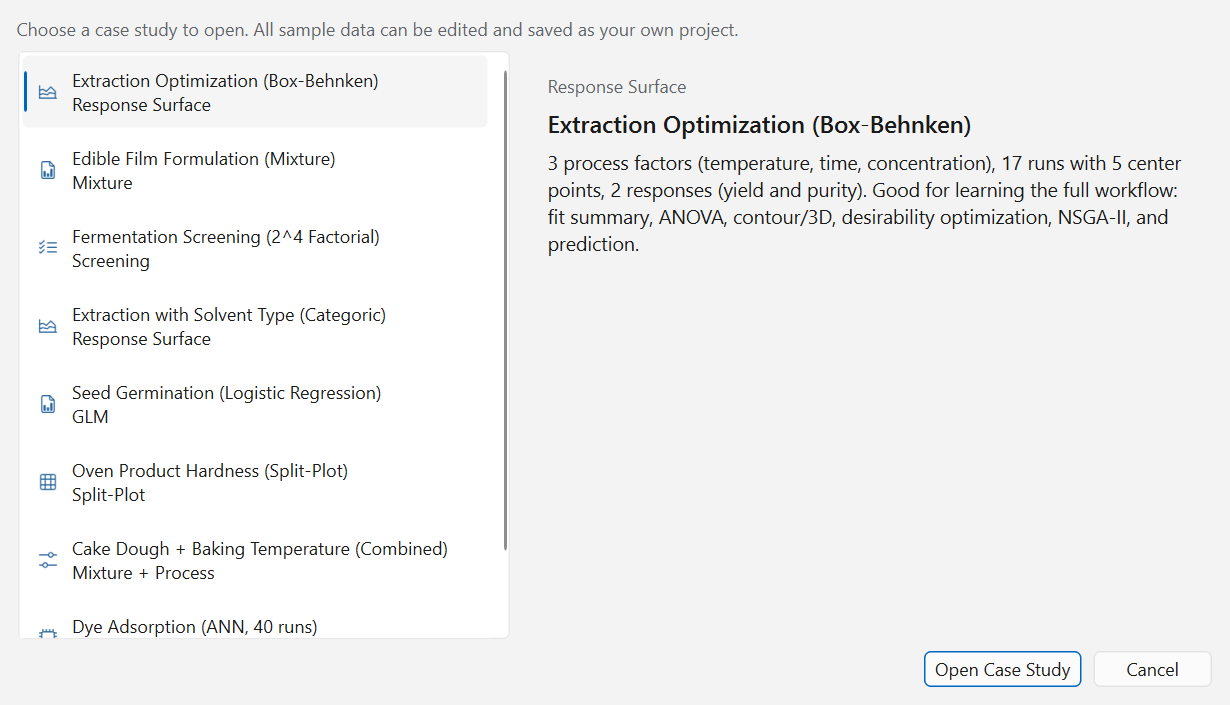
\includegraphics[width=0.75\linewidth]{case_studies.png}
\caption{The \ui{Case Studies} dialog with the BBD extraction case selected.}
\label{fig:ch11-cases}
\end{figure}

The \ui{Data} page shows a Box-Behnken design with three numeric factors, Temperature (60--80~°C), Time (30--90~min)
and Concentration (1--3~\%), 17 runs including 5 center points, and the responses Yield (\%) and Purity (\%). The goal
of the study is to maximize both.

\subsection{Data readiness}
Open \ui{Data Readiness} (Figure~\ref{fig:ch11-readiness}). With the reference model Quadratic (10 parameters) both
responses are rated \ui{Ready}: Yield scores 94 for modeling and 96 for optimization, Purity 100 and 97. The checks
behind the scores:
\begin{itemize}
  \item 17 complete runs, residual df 7, three levels per factor, pure error df 4, maximum VIF 1.01, largest gap
        in the factor space 0.27: the design is sound.
  \item Yield has two influential runs (runs 1 and 7, Cook's distance $>1$) and a significant lack of fit
        (p 0.030), both marked \ui{Needs attention}. The signal-to-noise ratio is 15.4.
  \item The optimization readiness is good: model $p=1.7\times10^{-6}$, predicted $R^2$ 0.886, the model-predicted
        maximum of Yield (75.46~°C, 86.13~min, 2.298~\%) lies inside the region, at a distance of 0.16 from the
        nearest run.
\end{itemize}
The recommendations are to check runs 1 and 7 for recording errors and, because of the lack of fit, to consider a
higher-order model, a transform or an ANN. Runs 1 and 7 belong to the design and there is no record of a problem, so
they stay in the analysis; the lack of fit is discussed below.

\begin{figure}[htbp]
\centering
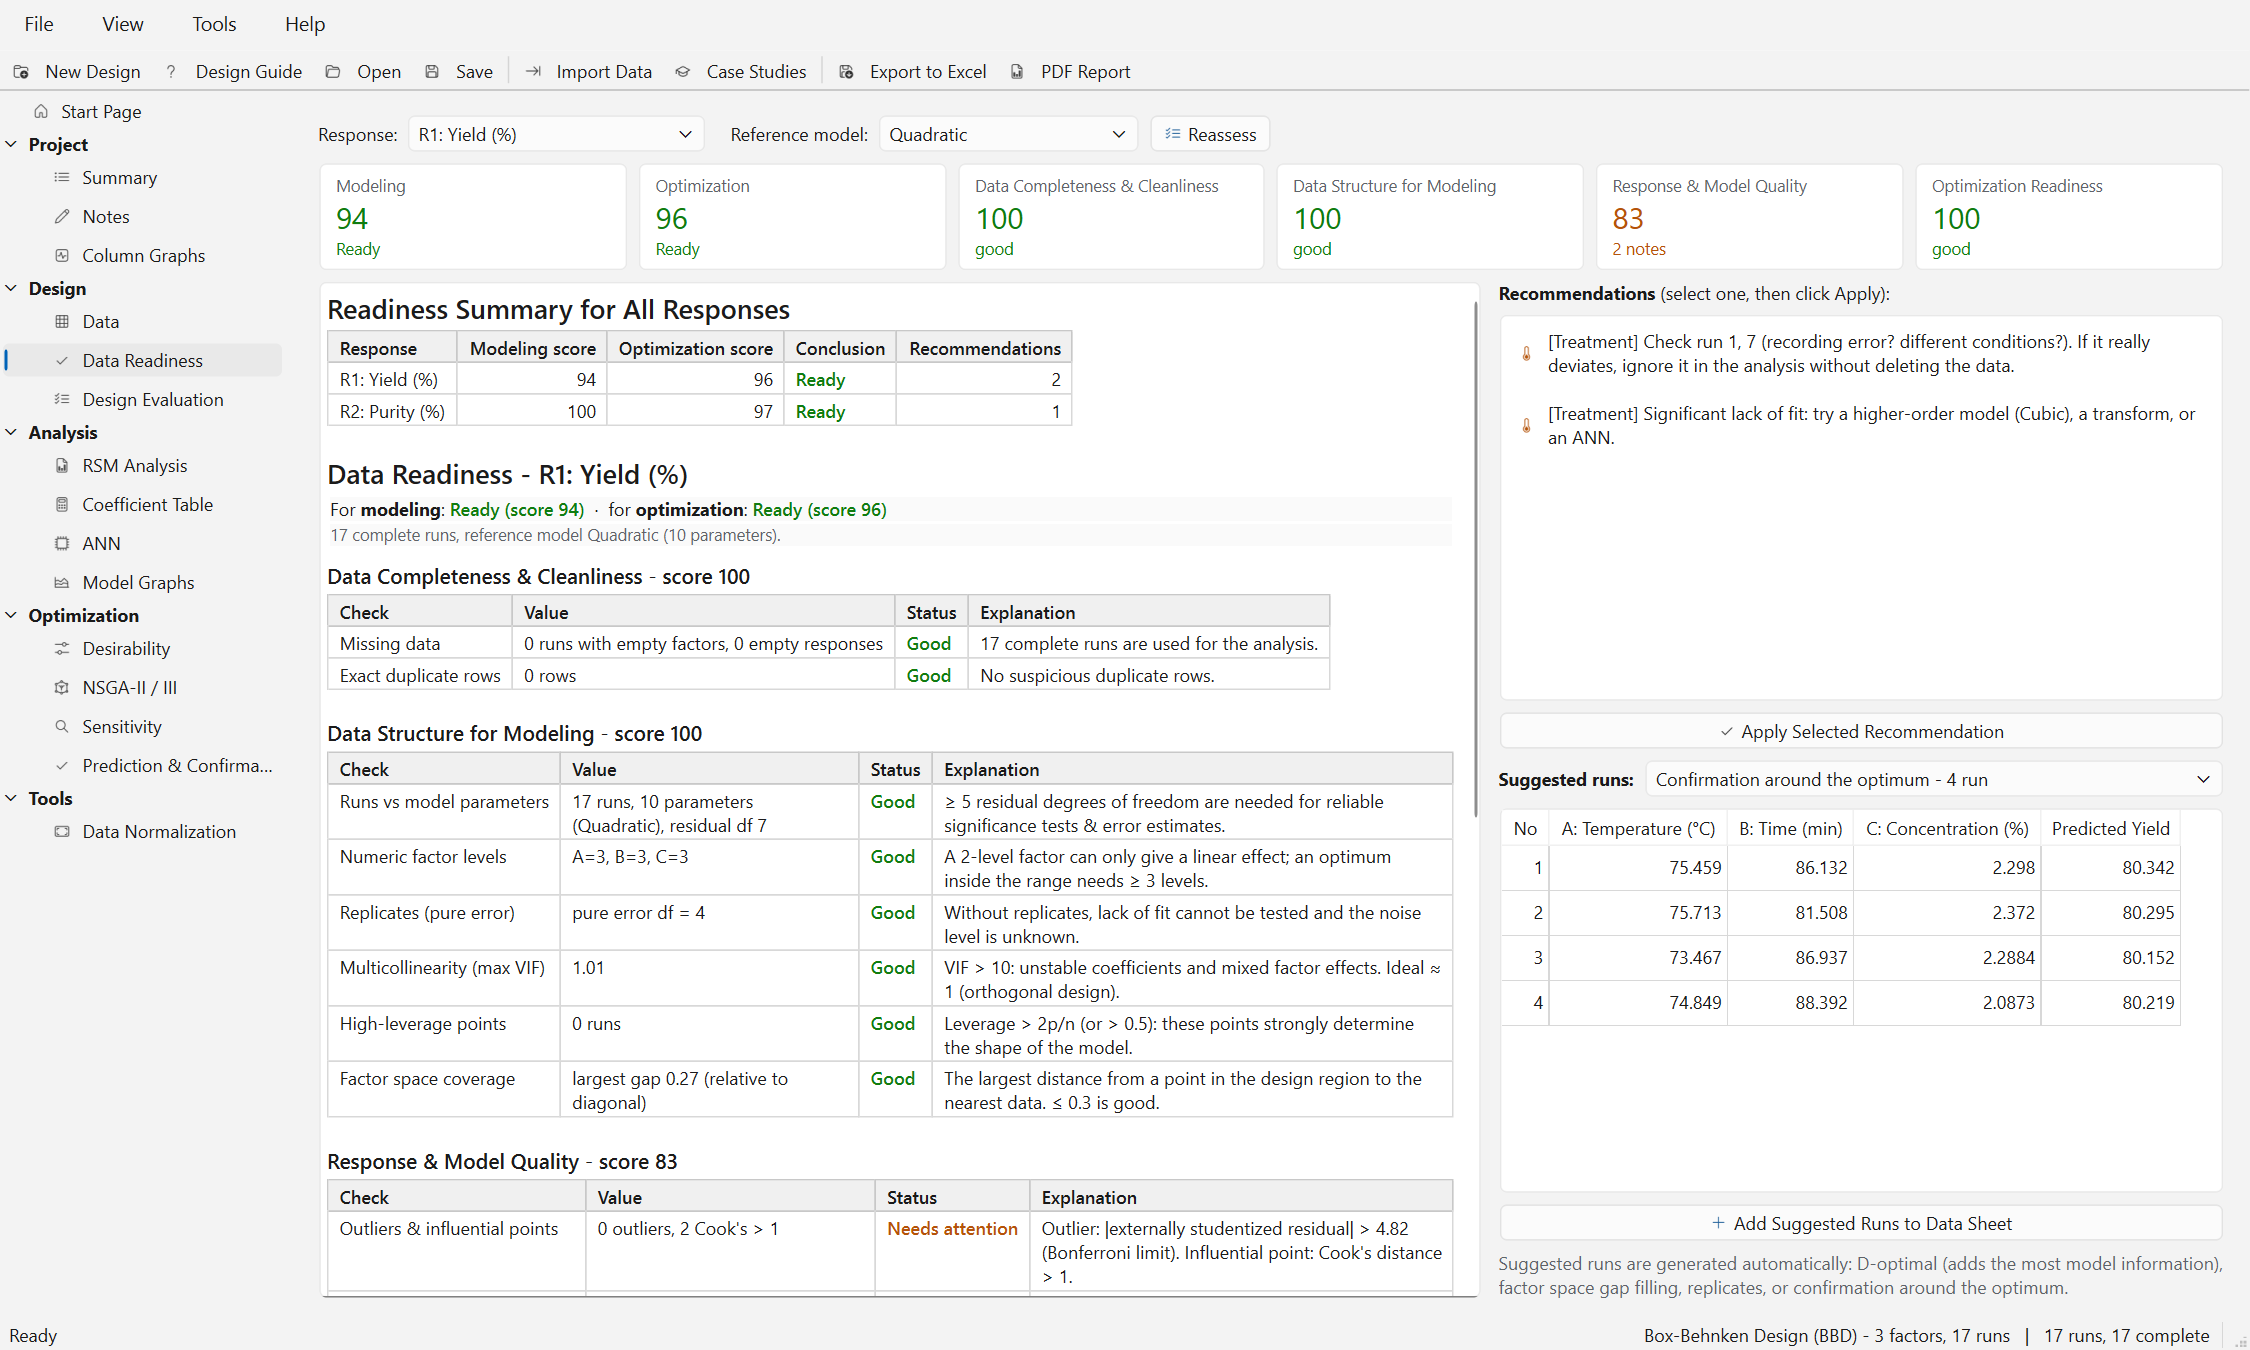
\includegraphics[width=\linewidth]{readiness.png}
\caption{\ui{Data Readiness} of the BBD case: both responses \ui{Ready}.}
\label{fig:ch11-readiness}
\end{figure}

% ======================================================================================================
\section{Part A: fit the response surface models}
\label{sec:ch11-rsm}

\subsection{Model selection and ANOVA}
On \ui{RSM Analysis}, tab \ui{Fit Summary}, the sequential model comparison for Yield suggests the quadratic model
(sequential $p<0.0001$, adjusted $R^2$ 0.9815, predicted $R^2$ 0.8857); the cubic model is aliased in a BBD. The
page marks the suggestion with \ui{Significant lack of fit} and warns ``the suggested model (Quadratic) has significant
lack of fit (p = 0.0302)''; the lack of fit is examined with the ANOVA below. Use the suggested model (\ui{Use
Suggested Model}) for both responses.

\begin{figure}[htbp]
\centering
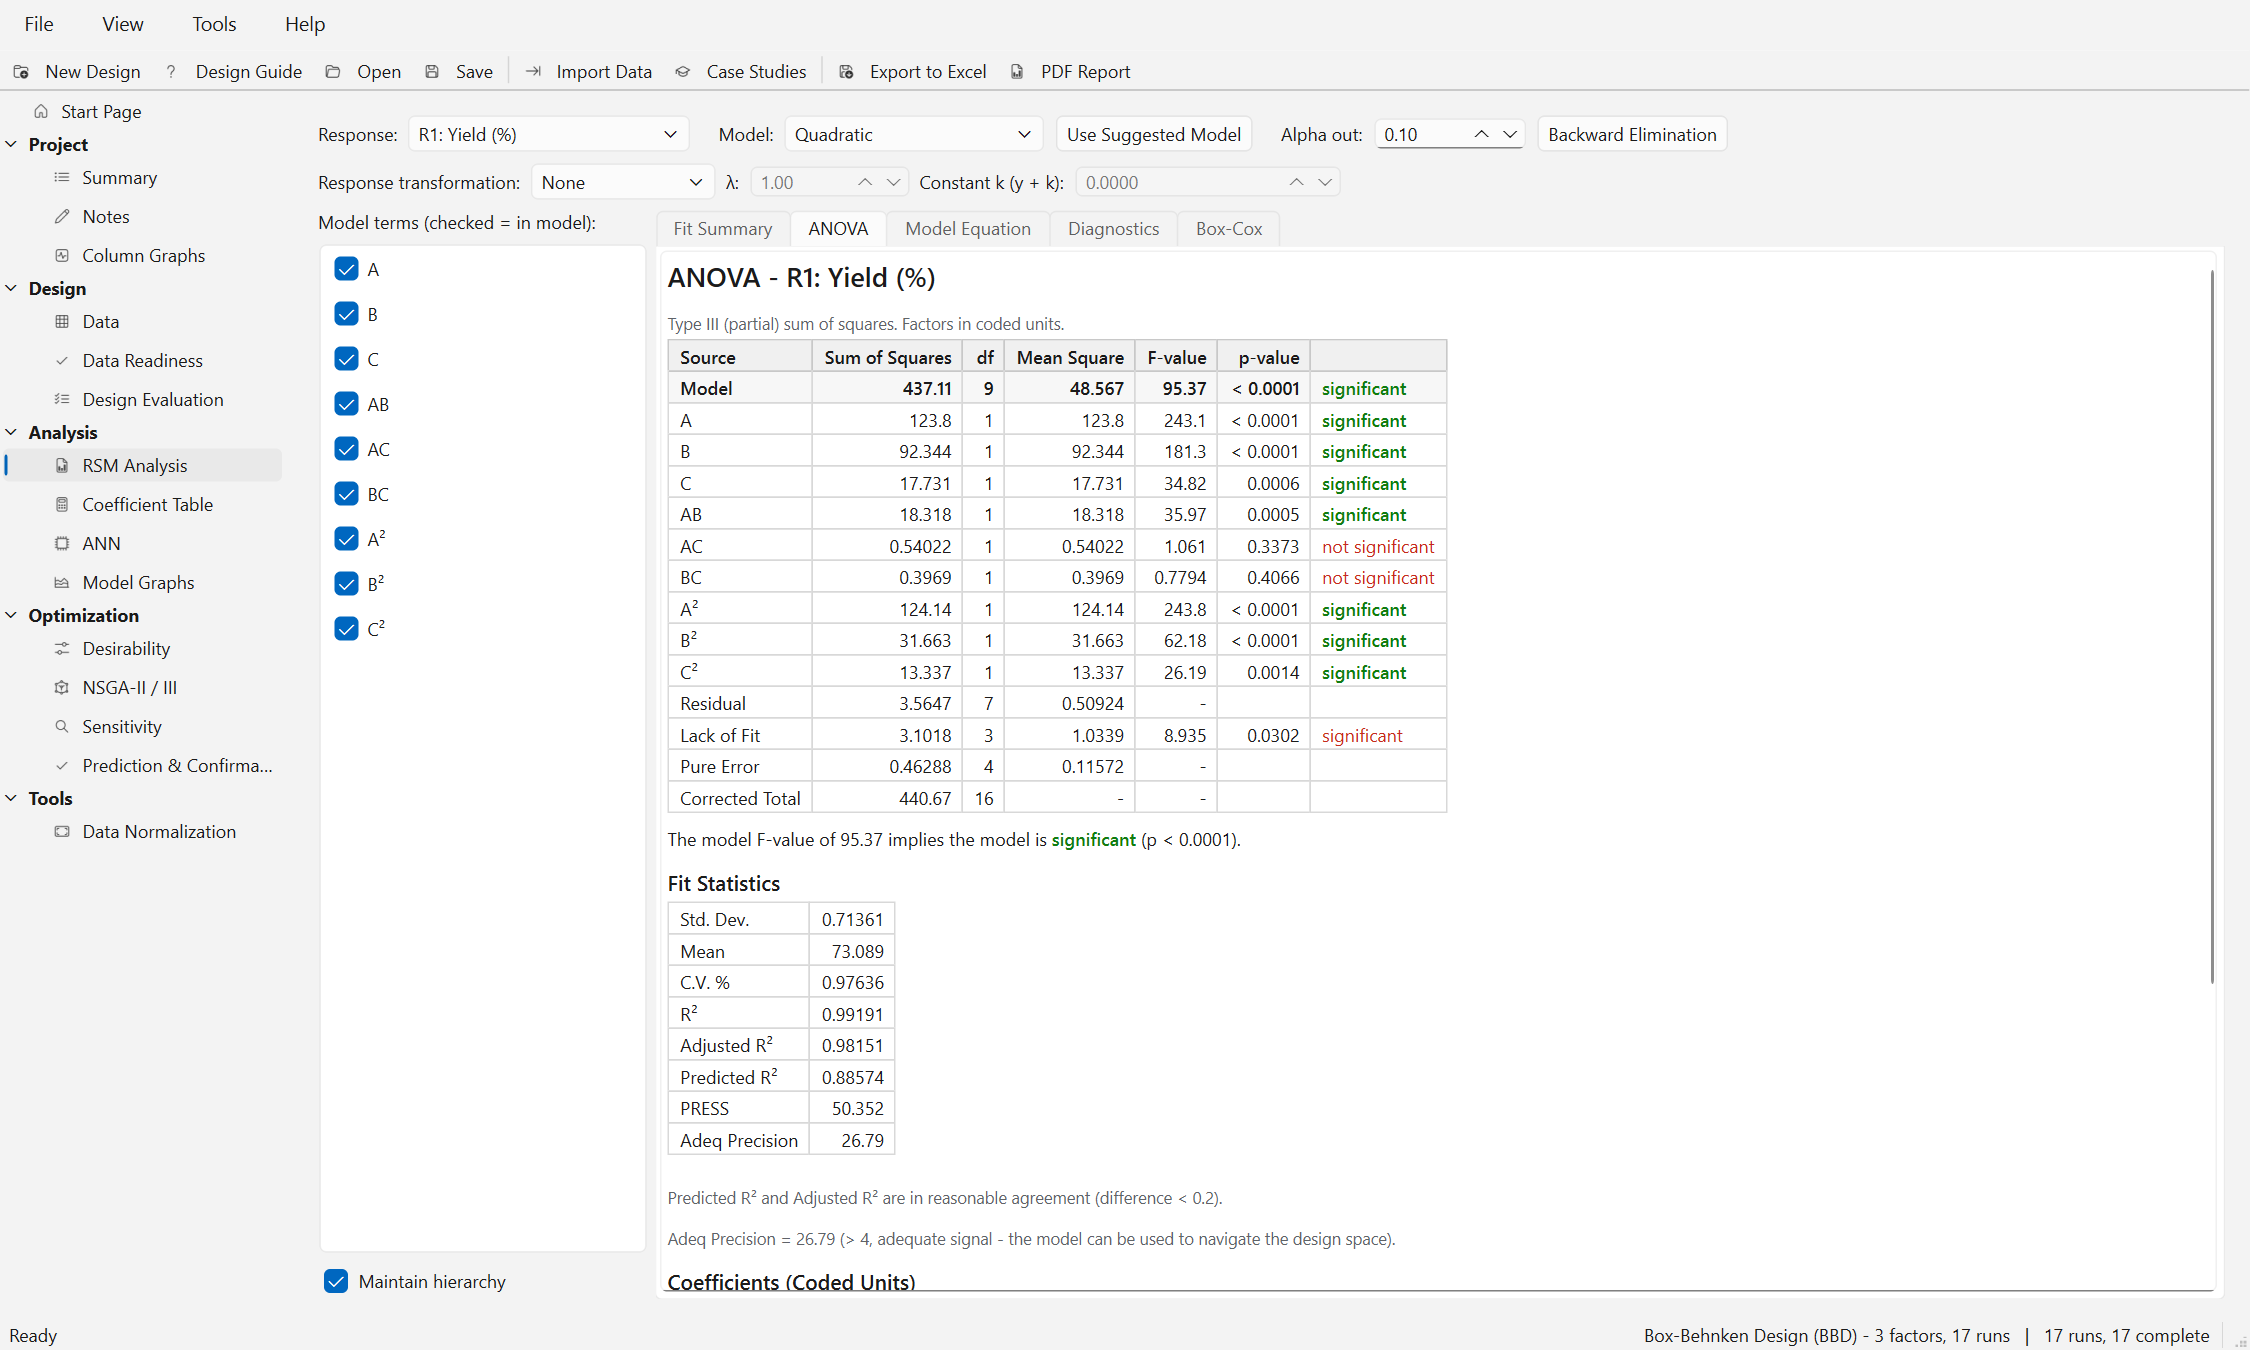
\includegraphics[width=\linewidth]{rsm_anova.png}
\caption{ANOVA of the quadratic model for Yield.}
\label{fig:ch11-anova}
\end{figure}

The \ui{ANOVA} tab for Yield (Figure~\ref{fig:ch11-anova}) gives:
\begin{itemize}
  \item Model $F=95.37$, $p<0.0001$; $R^2=0.9919$, adjusted $R^2=0.9815$, predicted $R^2=0.8857$, Adeq Precision 26.79,
        standard deviation 0.714, C.V. 0.98~\%.
  \item All linear and quadratic terms and the AB interaction are significant; AC ($p=0.337$) and BC ($p=0.407$) are
        not. Removing them would change the predictions very little; the full quadratic model is kept here so that
        both responses use the same model form.
  \item Lack of fit $F=8.935$, $p=0.0302$: significant. The pure error (mean square 0.116, 4 df from five center
        points) is very small compared with the lack-of-fit mean square (1.03). With such a precise replicate
        estimate, even small systematic deviations from the quadratic surface become significant. The lack-of-fit
        mean square corresponds to a standard deviation of about 1 percentage point of Yield, which is small relative to the response
        range (64.1--78.3), and the predicted $R^2$ of 0.886 shows that the model predicts new runs well. We accept
        the model and keep the lack of fit in mind: it is one reason to try an ANN (and to run check~D).
\end{itemize}
The equation in coded factors is
$\text{Yield}=77.772+3.934A+3.398B+1.489C+2.140AB-0.368AC-0.315BC-5.430A^2-2.742B^2-1.780C^2$.

For Purity the quadratic model gives $R^2=0.9886$, adjusted $R^2=0.974$ and predicted $R^2=0.9302$, with an
insignificant lack of fit ($p=0.638$). Temperature lowers Purity ($-2.354$ per coded unit), Time raises it.

\subsection{Diagnostics}
On \ui{Diagnostics} the normal plot of the externally studentized residuals is straight (Shapiro--Wilk $p=0.904$), no
residual exceeds the Bonferroni limit $\pm4.82$, and only runs 1 and 7 have Cook's distance above 1, the same runs as in
the readiness report. \ui{Box-Cox} recommends no transformation ($\lambda=1$ lies inside the confidence interval).
The models are adequate for optimization.

% ======================================================================================================
\section{Part A: ANN with checks A and B}
\label{sec:ch11-ann-bbd}
The lack of fit of Yield raises the question whether an ANN would do better. With 17 runs that is doubtful, and the
checks of REGEN make the answer explicit.

\begin{enumerate}
  \item Open \ui{ANN}. The \ui{Data Adequacy} report runs automatically: Yield is \ui{Adequate with caveats} (only 17
        runs, \ui{Caution}; training rows per weight 1.27, \ui{Caution}; signal/noise 15.43 and the significant lack of
        fit rate the need for a nonlinear model as \ui{Good}). Purity is \ui{Adequate with many caveats - ANN results
        need strict validation}: in addition run 8 is a response outlier (robust $z>3.5$).
  \item Set \ui{CPU cores (parallel):} to 1 if you want exactly the numbers below, leave the other settings at their
        defaults and click \ui{Optimize All Responses (One Click)}. This is \textbf{check~A}: a cross-validated
        architecture search for each response.
  \item Select each response in \ui{Show response:} and click \ui{Learning Curve (Enough Data?)}. This is
        \textbf{check~B}.
\end{enumerate}

\textbf{Check~A result.} The status line reads \ui{Done. R1: 1 layer (4) - Good fit; R2: 1 layer (5) - Good fit}.
For Yield, 26 architectures were evaluated with 5-fold cross-validation; the selected 3-4-1 network (21 weights) has a
cross-validated training $R^2$ of 0.971 and test $R^2$ ($Q^2$) of 0.624. A 3-4-5-1 network had a slightly lower test
error, but within one standard error, so the simpler network was kept (1-SE rule). 21 candidates were excluded as
overfitting. On the same folds the quadratic RSM reaches $Q^2=0.598$, so the search reports \ui{ANN predicts new data
better than RSM (assessed on the same test data)}, but the margin (0.624 against 0.598) is small. For Purity the
selected 3-5-1 network has $Q^2=0.774$, while RSM reaches 0.818: \ui{RSM predicts new data as well as or better than
ANN}.

The \ui{Summary \& Diagnosis} tab of the Yield network shows \ui{Good fit (result of 5-fold cross-validation during
architecture search)} and, as secondary information, the single train/test split of the final model (11 training,
3 validation, 3 test runs): \ui{Overfitting}, test $R^2=-0.75$. The page itself warns that 6 validation and test runs
are too few for this diagnosis; the cross-validated result is the one to use.

\textbf{Check~B result.} For both responses the learning curve ends with \ui{Learning curve finished: too little data
to assess}: \ui{Too little data (17 runs) for a reliable learning curve.} With the full data the ANN test $R^2$
(median of 10 repeats on 3 test runs) is 0.552 for Yield and 0.315 for Purity, against 0.885 and 0.911 for RSM:
\ui{RSM is more accurate at this data size}.

\textbf{Conclusion of checks A and B for Part A.} The networks are not badly overfitted, but 17 runs do not support an
ANN that is clearly better than the quadratic model. The RSM models remain the selected models (the check box
\ui{When finished, use ANN for graphs/optimization} was left off). The ANNs are kept only for check~D.

% ======================================================================================================
\section{Part A: set goals and run the desirability optimization}
\label{sec:ch11-desir}
On \ui{Desirability} set both responses to \ui{Maximize}. Raise the lower limits to the values below which a result
is of no interest, 75 for Yield and 89 for Purity; keep the upper limits at the data maxima (78.29 and 93.6), shape
1.00, importance \ui{+++} and model \ui{RSM}. Click \ui{Run Optimization}.

The result (Figure~\ref{fig:ch08-desirability} in Chapter~\ref{chap:8}) has five solutions with $D=0.845$--$0.862$. The best is
70.265~°C, 89.781~min, 1.7975~\% with predicted Yield 78.29 ($d=1$) and Purity 92.416 ($d=0.743$), $D=0.862$. Yield is
at its upper limit, so it is ``fully desirable''; all remaining freedom is used for Purity.

% ======================================================================================================
\section{Part A: NSGA-II and check C}
\label{sec:ch11-nsga}
On \ui{NSGA-II / III} the goals are already \ui{Maximize} for both responses (taken from the \ui{Desirability} page).
Keep all defaults and click \ui{Run Optimization}. Then click \ui{Check Population Size}.

\begin{itemize}
  \item The automatic algorithm choice is NSGA-II (two objectives). The run stops automatically at generation 78 with
        99 Pareto solutions (Figure~\ref{fig:ch08-front}). The front runs from Purity 94.9 at Yield 63.6 to Purity 89.6
        at Yield 80.4.
  \item TOPSIS chooses 71.527~°C, 88.239~min, 1.8783~\% (Yield 79.157, Purity 91.802); the knee point is 67.781~°C,
        89.982~min, 1.5083~\% (Yield 75.766, Purity 93.483).
  \item \textbf{Check~C, generations}: the convergence criterion was first met at generation 58, and in the last window
        the mean hypervolume changed by $-0.029$~\% (limit 0.10~\%) with no shift of the ideal point:
        \ui{Enough generations} (Figure~\ref{fig:ch08-convergence}).
  \item \textbf{Check~C, population}: two other seeds change the hypervolume by at most 0.02~\%, a population of 200
        adds 0.35~\%: \ui{Population: sufficient} (Table~\ref{tab:ch08-popcheck}). The TOPSIS choice moves by at most
        5.5~\% of a factor range between these runs.
\end{itemize}
Check~C is passed. Note how desirability and NSGA relate: the best desirability solution (Yield 78.29, Purity 92.42)
lies on the NSGA front between the knee and the TOPSIS point. The desirability result depends on the limits you chose;
the front shows what other compromises are available.

% ======================================================================================================
\section{Part A: compare the ANN and RSM fronts (check D)}
\label{sec:ch11-checkD}
Click \ui{Compare ANN vs RSM}. The optimization runs twice, with RSM and with the ANNs of
Section~\ref{sec:ch11-ann-bbd}. The results are shown in Figures~\ref{fig:ch08-cmp-front}--\ref{fig:ch08-cmp-report}
of Chapter~\ref{chap:8}:
\begin{itemize}
  \item Mean prediction difference on the Pareto solutions: 22.4~\% of the data range for Yield (maximum 78.0~\%),
        4.3~\% for Purity.
  \item TOPSIS choices: RSM front 71.5~°C, 88.2~min, 1.88~\%; ANN front 65.3~°C, 90.0~min, 3.00~\%; distance
        $dx=56$~\% of the factor range.
  \item Hypervolume: 71.5~\% (RSM front, by RSM) and 82.4~\% (ANN front, by ANN); re-assessed by the other model 69.0~\%
        and 57.6~\%.
  \item Prediction accuracy on new data: RSM mean predicted $R^2$ 0.908 against ANN mean cross-validation $Q^2$
        0.699.
\end{itemize}
\textbf{Check~D fails} with the red verdict \ui{The models differ considerably: \dots\ Do not rely on just one model:
make confirmation runs at both TOPSIS points.}

\textbf{What it means.} At its TOPSIS point the ANN predicts a Yield of 83.5, more than 5 units above the highest
Yield ever measured (78.29), at a corner of the region (Time 90~min, Concentration 3~\%) where the BBD has no run. The
RSM predicts 74.0 there. One of the two models extrapolates badly, and the evidence points to the ANN: checks A and B
showed that 17 runs do not support it, its cross-validated $Q^2$ (0.62 and 0.77) is lower than the RSM predicted $R^2$
(0.89 and 0.93), and its front loses much more hypervolume when re-assessed (82.4 to 57.6~\%) than the RSM front (71.5
to 69.0~\%).

\textbf{Action.} The optimum is taken from the RSM models. The disagreement is reported, and the confirmation plan
(Section~\ref{sec:ch11-predict}) includes a run at the ANN TOPSIS point, which settles the question with little effort.

% ======================================================================================================
\section{Part A: sensitivity and parametric study}
\label{sec:ch11-sens}
On \ui{Sensitivity} choose \ui{Start from:} \ui{Best desirability solution} and \ui{Model:} \ui{Selected model of
each response}. Run the four studies (details in Chapter~\ref{chap:9}):
\begin{itemize}
  \item \ui{Parametric Study}, \ui{All factors, one panel each} (Figure~\ref{fig:ch09-param-all}): Temperature
        creates the conflict; between 60 and 80~°C Yield rises from 66.6 to 79.9 (at 76~°C) while Purity falls from
        94.1 to 87.3.
  \item \ui{Global Sensitivity}, Sobol indices with $N=8192$ (Figure~\ref{fig:ch09-sobol}): Temperature dominates
        both responses ($S_T=0.599$ for Yield, 0.714 for Purity); Time is second for Yield (0.364) and Concentration for
        Purity (0.151); interactions account for about 4~\% of the variance. The standardized coefficients
        (Figure~\ref{fig:ch09-src}) have $R^2=0.70$ for Yield, too low to rank the factors by $\beta$ alone.
  \item \ui{Local Sensitivity (Tornado)}, $\pm10$~\% (Figure~\ref{fig:ch09-tornado}): at the chosen setting
        Temperature must be controlled most tightly (Yield swing 2.34, Purity swing $-1.40$ for $\pm2$~°C).
  \item \ui{Pareto Front Trade-off} (Figure~\ref{fig:ch09-front}): moving along the front means moving Temperature
        and Concentration together ($\rho=\pm0.998$ and $\pm0.980$); Time stays at about 90~min.
\end{itemize}
For the paper, these results support a simple statement: Temperature sets the balance between Yield and Purity, Time
should be long, and Concentration fine-tunes Purity.

% ======================================================================================================
\section{Part A: prediction and confirmation plan}
\label{sec:ch11-predict}
On \ui{Desirability} select solution~1 and click \ui{Send Selected Solution to Prediction}. The \ui{Prediction \&
Confirmation} page (Figure~\ref{fig:ch11-prediction}, 95~\% level, $n=3$ confirmation runs) shows:
\begin{itemize}
  \item Yield: prediction 78.29, standard error of the mean 0.430, CI 77.27--79.31, PI for the mean of 3 runs
        76.88--79.70;
  \item Purity: prediction 92.42, standard error 0.224, CI 91.89--92.95, PI 91.68--93.15.
\end{itemize}
The PI is the interval that the mean of the three confirmation runs should fall into if the model is right. In the
screenshot, example confirmation means (78.69 and 92.12) have been typed in to show the result \ui{\checkmark\ Confirmed
(inside PI)}; in a real study you enter your measured means.

\begin{figure}[htbp]
\centering
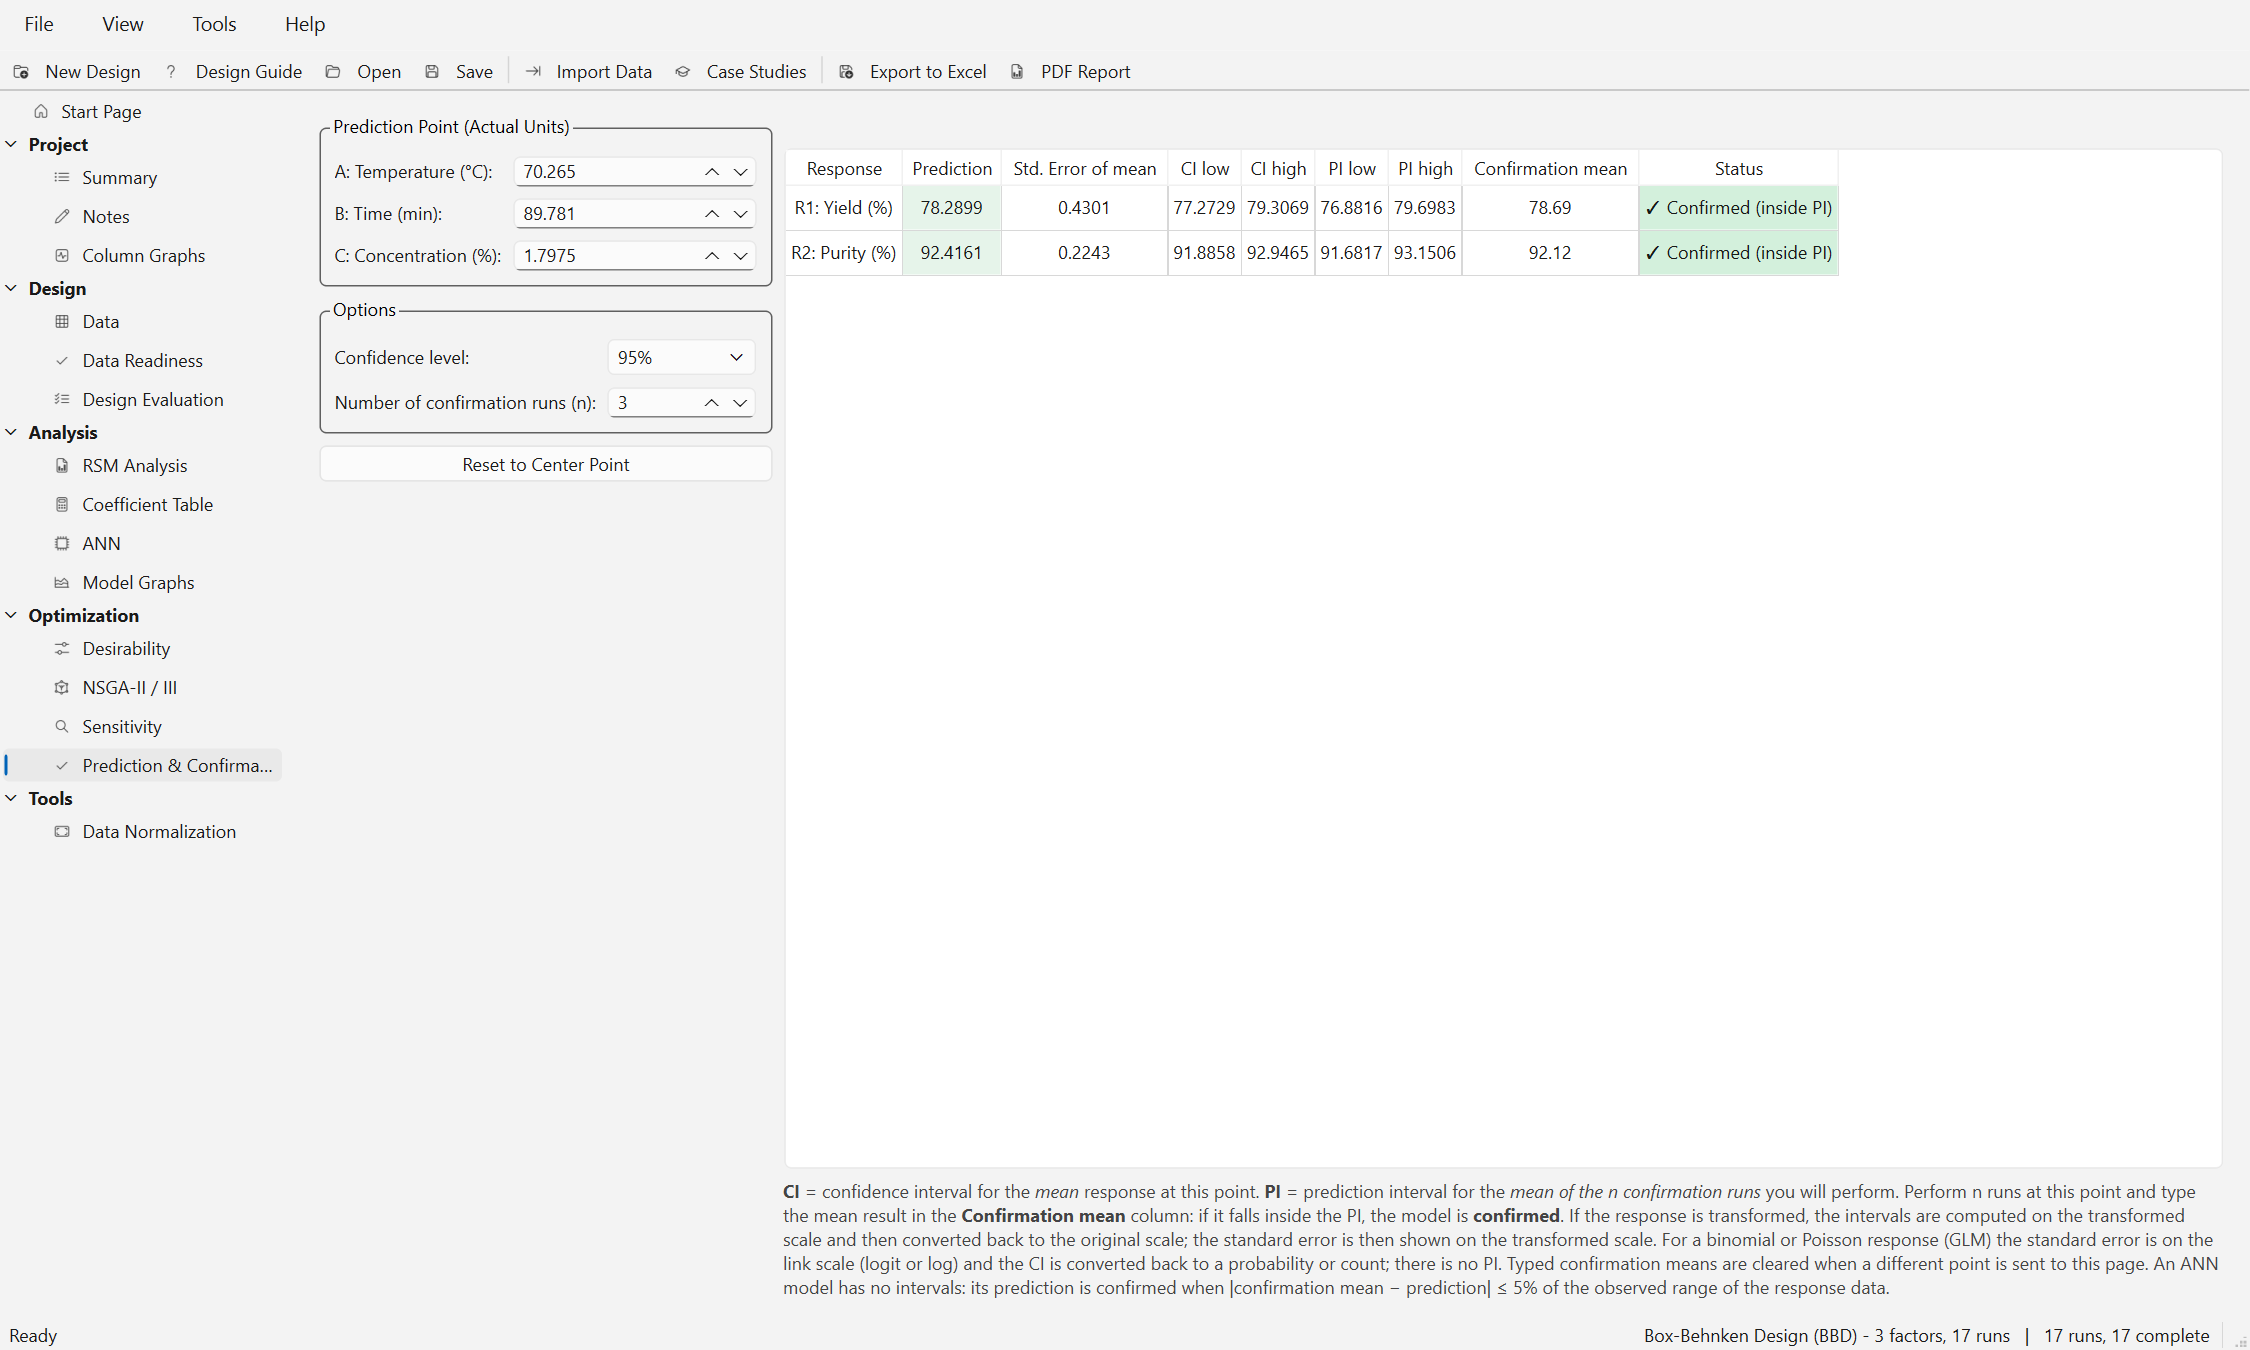
\includegraphics[width=\linewidth]{prediction.png}
\caption{\ui{Prediction \& Confirmation} for the best desirability solution, 95~\%, $n=3$. The confirmation means are
example values.}
\label{fig:ch11-prediction}
\end{figure}

\textbf{Confirmation plan.} Because check~D failed, the plan contains two settings:
\begin{enumerate}
  \item Three runs at the chosen optimum (70.3~°C, 89.8~min, 1.80~\%). Accept the RSM model if both means fall inside
        the PIs above.
  \item One to three runs at the ANN TOPSIS point (65.3~°C, 90.0~min, 3.00~\%). Enter this point on the prediction
        page: the RSM predicts Yield 73.97 with a PI (3 runs) of 72.1--75.8, whereas the ANN predicts 83.5. A measured
        Yield near 74 confirms the RSM and refutes the ANN's promise; a Yield near 83 would mean the RSM misses a
        better region and the design should be extended toward high Concentration.
\end{enumerate}
The \ui{Data Readiness} page also proposes confirmation runs around the optimum (\ui{Add Suggested Runs to Data
Sheet}). After the runs, enter the results on the \ui{Data} page, refit and repeat the checks.

% ======================================================================================================
\section{Part B: dye adsorption, when an ANN is justified}
\label{sec:ch11-dye}
Open \ui{Dye Adsorption (ANN, 40 runs)} from \menupath{File $\rightarrow$ Case Studies\dots}. The data are 40
historical runs with four factors (pH 2--10, adsorbent dose 0.5--4~g/L, contact time 10--120~min, initial concentration
20--200~mg/L) and the response Removal Efficiency (\%).

\subsection{Readiness and RSM}
\ui{Data Readiness} rates the data \ui{Fair - some things need fixing} (modeling 82, optimization 77): there are no
replicates (pure error df 0, \ui{Problem}), so the noise level and the lack of fit cannot be assessed. The quadratic RSM
model (15 parameters) fits with $R^2=0.877$ but predicts new data poorly (predicted $R^2=0.562$): a sign that the
response is more nonlinear than a quadratic surface.

\subsection{Data adequacy}
On \ui{ANN} the \ui{Data Adequacy} verdict is \ui{Adequate with caveats}: 40 runs (\ui{Good}), training rows per
weight 2.62 for a 4-2-1 reference network (\ui{Caution}), factor correlation at most 0.25 (\ui{Good}), skewed response
(skewness 0.85, max/min 21.4, \ui{Caution}), and no replicates for the signal-to-noise ratio (\ui{Info}). For the
skewed response the page points out that a ln transform on the \ui{RSM Analysis} page would change only the RSM model:
the ANN is trained on the response in its original units.

\subsection{Check B: learning curve}
Click \ui{Learning Curve (Enough Data?)} with the default network entry ``5'' (one hidden layer with 5 neurons)
(Figure~\ref{fig:ch11-lc}). The ANN is trained on 30 to 100~\% of the training data (10 to 32 runs) and tested on
8 runs never used for training, repeated 10 times. The median test $R^2$ rises from about 0 at 10 runs to 0.898 at 26
and 0.876 at 32 runs; the RSM reaches only 0.429 on the same test runs. The page concludes \ui{More data would still
help} and estimates about 100 runs in total (range 95 to 111), but adds that this estimate is unreliable because the
fitted exponent lies at the edge of its search range. Read check~B here as: the ANN already clearly beats the RSM with
40 runs, and more runs would still improve it; the exact number of runs is uncertain.

\begin{figure}[htbp]
\centering
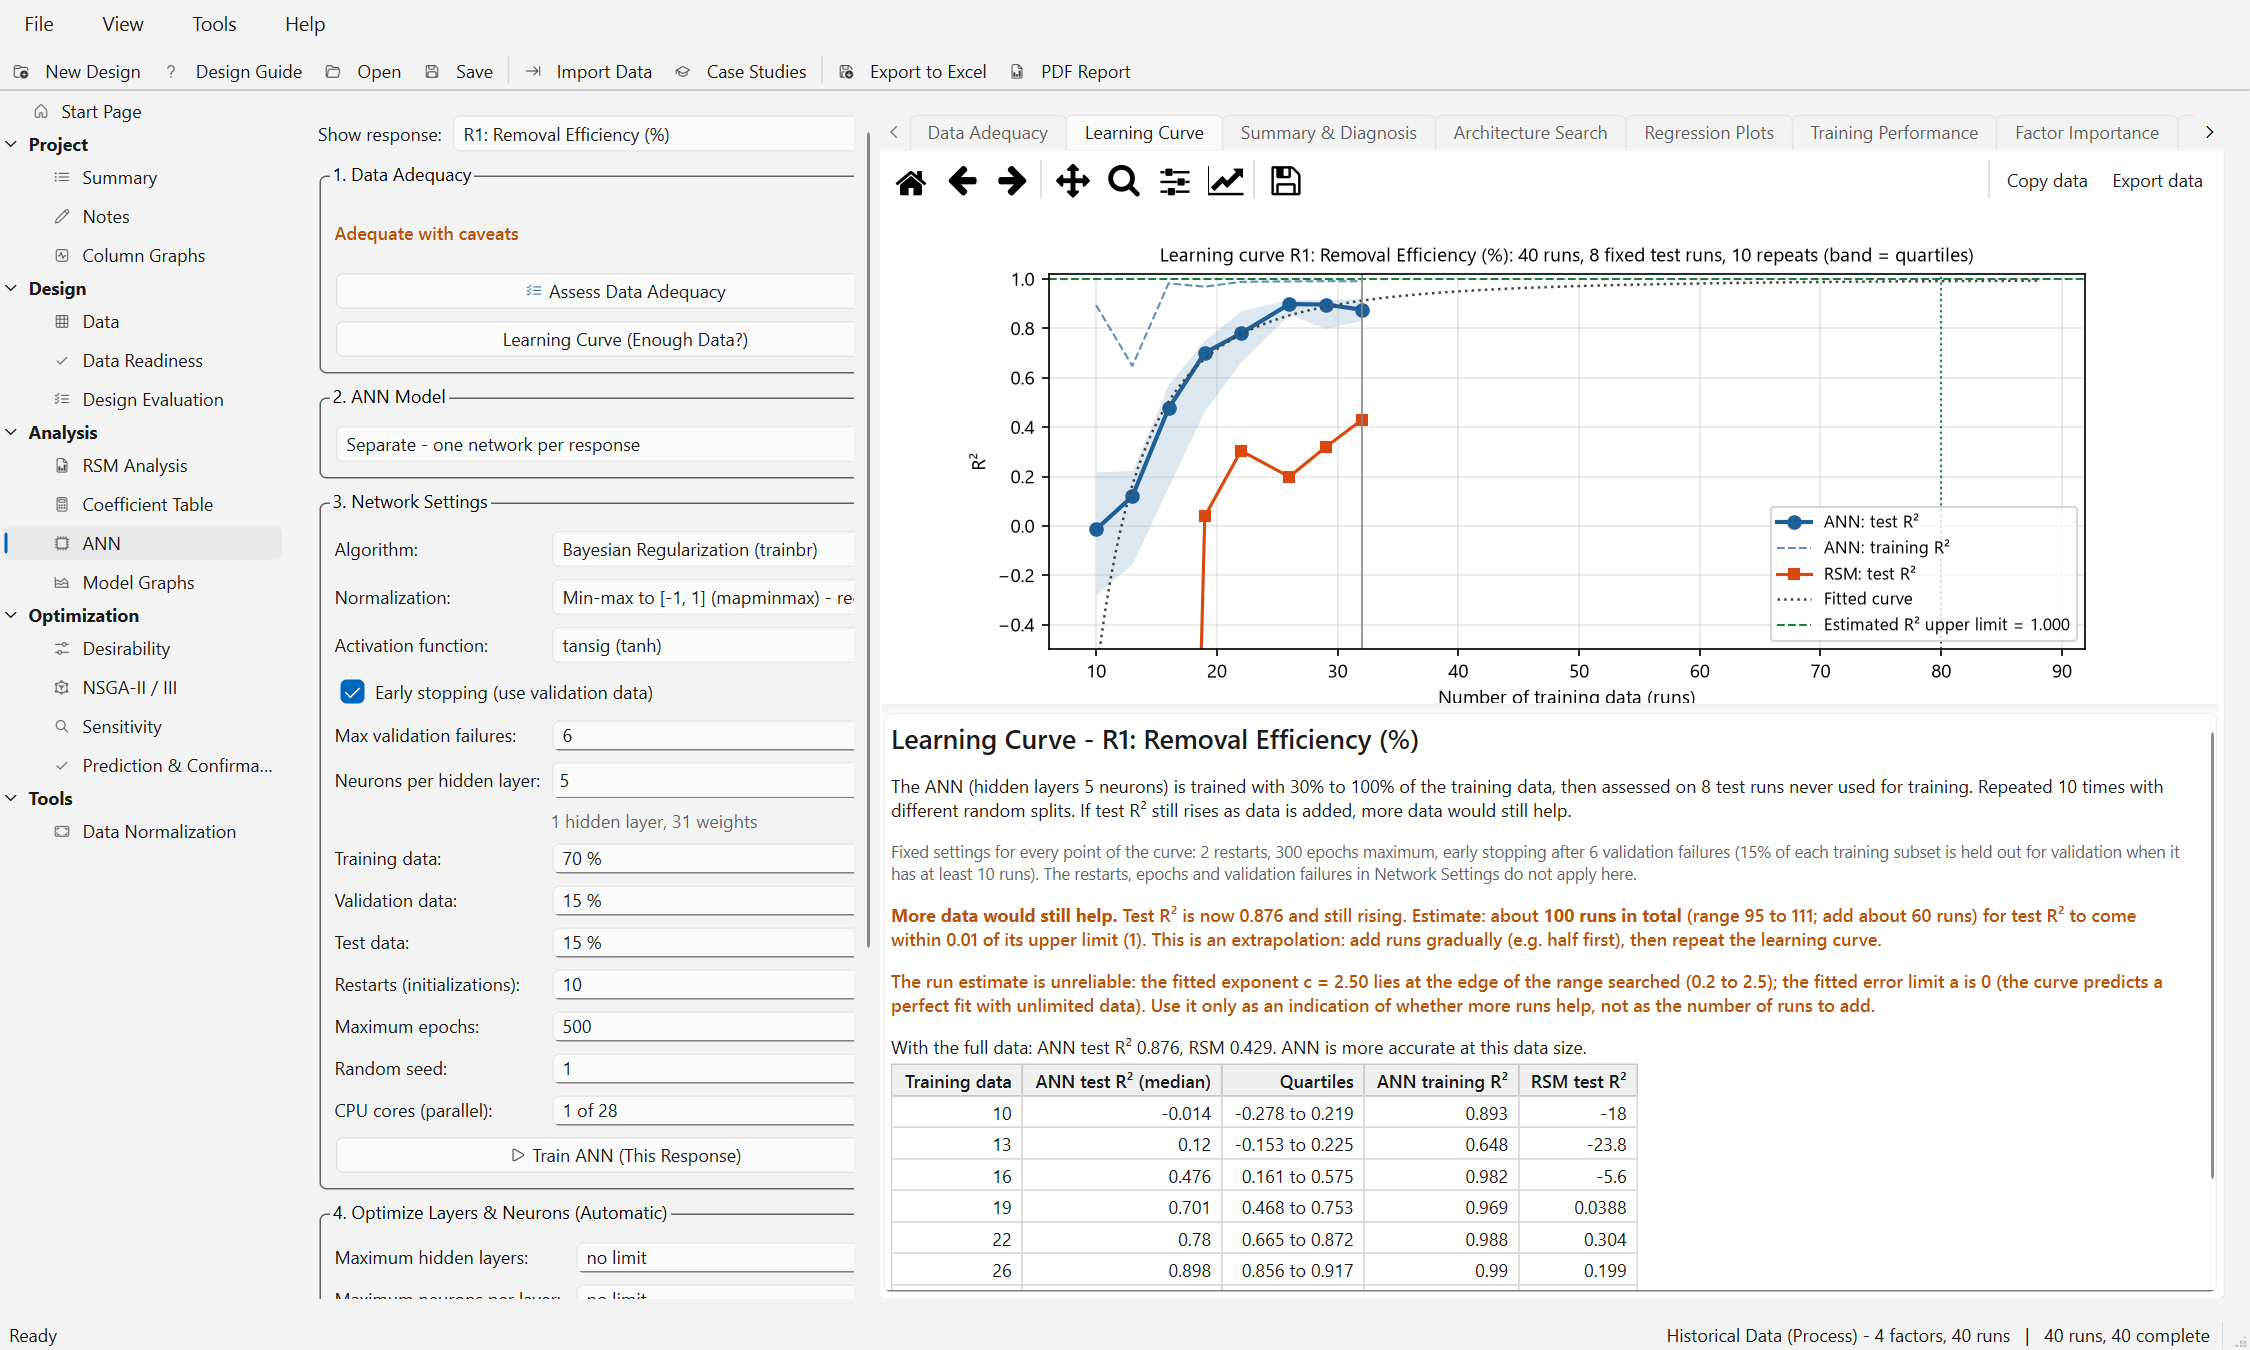
\includegraphics[width=\linewidth]{ann_learning_curve.png}
\caption{Check B for the dye case: learning curve of the ANN (test $R^2$ against training runs) compared with RSM.}
\label{fig:ch11-lc}
\end{figure}

\subsection{Check A: architecture search}
Click \ui{Search Architecture (This Response)} with the default search settings (Figure~\ref{fig:ch11-search}). Fifteen
architectures are evaluated with 5-fold cross-validation. The first hidden layer stops growing at 5 neurons, and a
second layer does not improve the test error by 1~\%. The selected network is 4-3-1 (19 weights): cross-validated
training $R^2$ 0.987, test $R^2$ ($Q^2$) 0.938, \ui{Good fit}; the RSM reaches $Q^2=0.376$ on the same folds. Nine
candidates were excluded as overfitting and three as underfitting.

\begin{figure}[htbp]
\centering
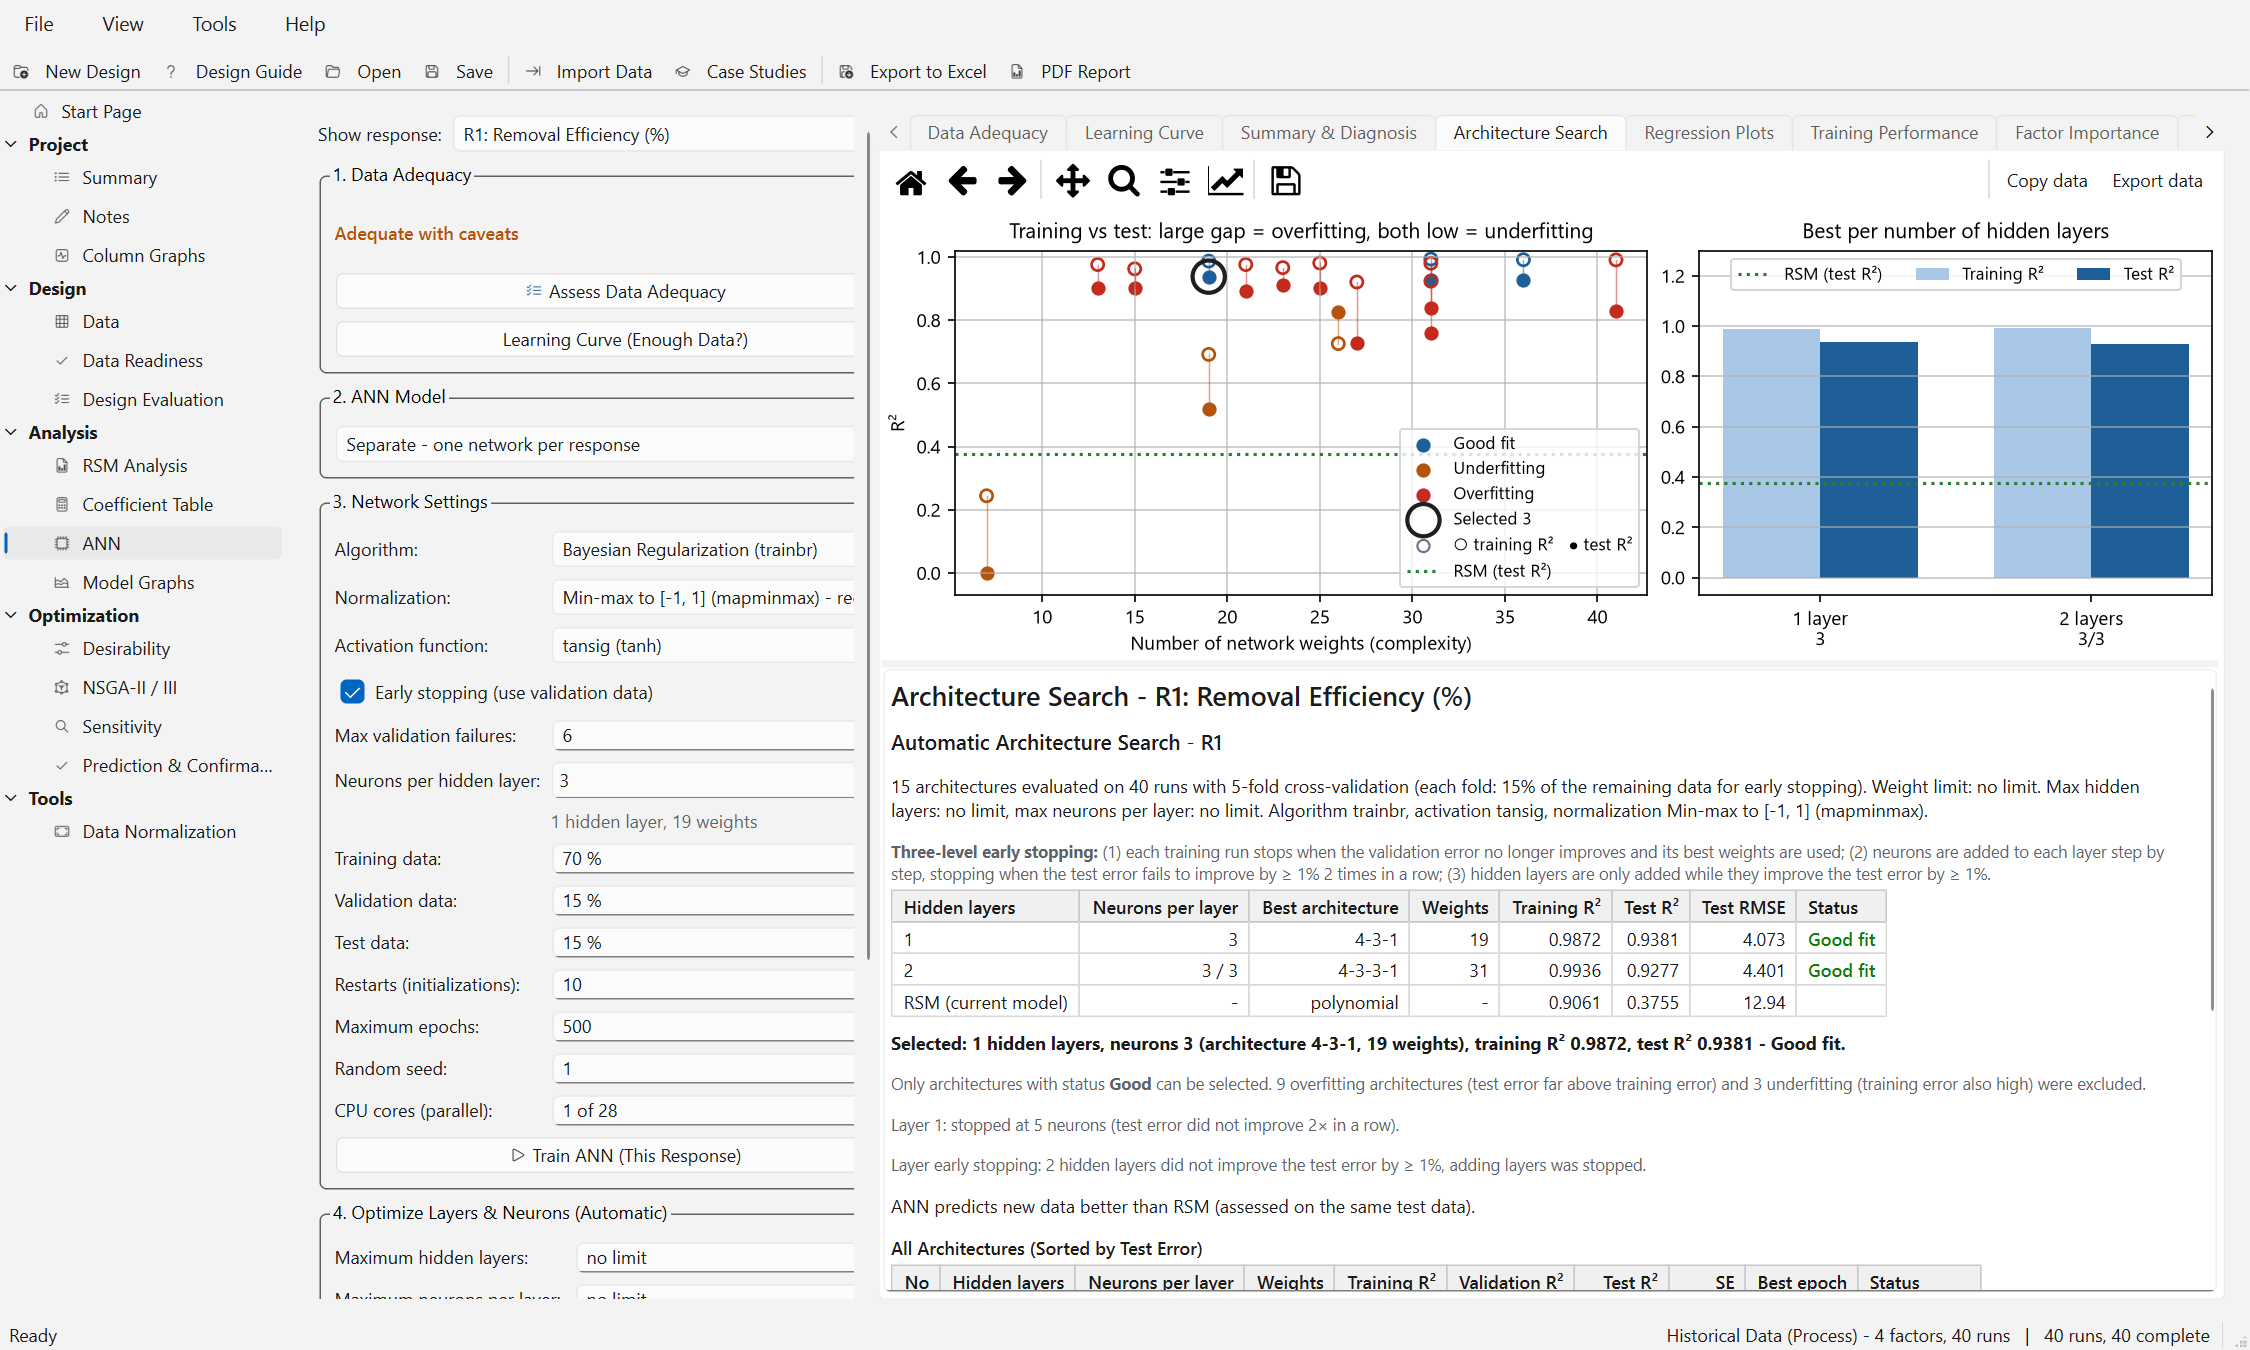
\includegraphics[width=\linewidth]{ann_search.png}
\caption{Check A for the dye case: architecture search with 5-fold cross-validation; selected network 4-3-1.}
\label{fig:ch11-search}
\end{figure}

The final 4-3-1 network is trained on a 28/6/6 split. The \ui{Summary \& Diagnosis} tab reports \ui{Good fit} from the
cross-validation and, for the single final split, \ui{Overfitting} (error on new data 3.6 times the training error,
test $R^2=0.853$). As in Part A, the cross-validated status is the diagnosis to use. The \ui{RSM vs ANN} tab gives
$R^2=0.961$ for the ANN against 0.877 for RSM on all data, and the \ui{Factor Importance (Garson)} tab ranks pH first
(68.2~\%), as expected for an adsorption process with a pH optimum.

\textbf{Conclusion of Part B.} Here an ANN is justified: enough data (40 runs), a clearly nonlinear response that the
quadratic model cannot capture ($Q^2$ 0.94 against 0.38), a network selected by cross-validation, and a learning curve
that confirms the advantage. To use the network for graphs, optimization and prediction, tick \ui{Use this response's
ANN for graphs, optimization, NSGA-II \& prediction}. Keep two limitations in mind: an ANN has no confidence or
prediction intervals, so on the prediction page a confirmation run is judged by the rule $|\bar y-\hat y|\le5$~\% of the
response data range; and the data have no replicates, so the noise level is unknown. Adding a few replicated runs and
the runs suggested by \ui{Data Readiness} would strengthen the model. Multi-objective optimization and check~D need at
least two responses and are therefore not part of this case.

% ======================================================================================================
\section{Export the data and the report}
\label{sec:ch11-export}
Everything shown in this chapter can be exported for a paper or a lab report:
\begin{itemize}
  \item every plot: \ui{Copy data} and \ui{Export data\dots} on the plot toolbar (right-click: \ui{Copy plot data},
        \ui{Export plot data\dots}); the data behind each panel are written to the clipboard, an Excel workbook (one
        sheet per series) or a CSV file, so the figure can be redrawn in another program;
  \item every result table: right-click, \ui{Export table\dots} (Excel or CSV) or \ui{Copy entire table (for Excel)};
  \item every report panel (ANOVA, check reports, sensitivity tables): right-click, \ui{Export all tables\dots};
  \item the Pareto front with settings and convergence history: \ui{Export Pareto to Excel\dots} on the NSGA page;
  \item the whole project: \menupath{File $\rightarrow$ Export to Excel\dots} and \menupath{File $\rightarrow$ PDF
        Report\dots}.
\end{itemize}
The \ui{Summary} page (Figure~\ref{fig:ch11-summary}) collects the state of the project: factor and response tables
(Yield and Purity both quadratic, \ui{Used RSM}), ``2 ANN models, desirability optimization results (5 solutions),
NSGA-II results (99 Pareto solutions)'' and the notes. Save the project (\menupath{File $\rightarrow$ Save}); the models,
optimization results, comparisons and search results are stored in the \texttt{.doe} file.

\begin{figure}[htbp]
\centering
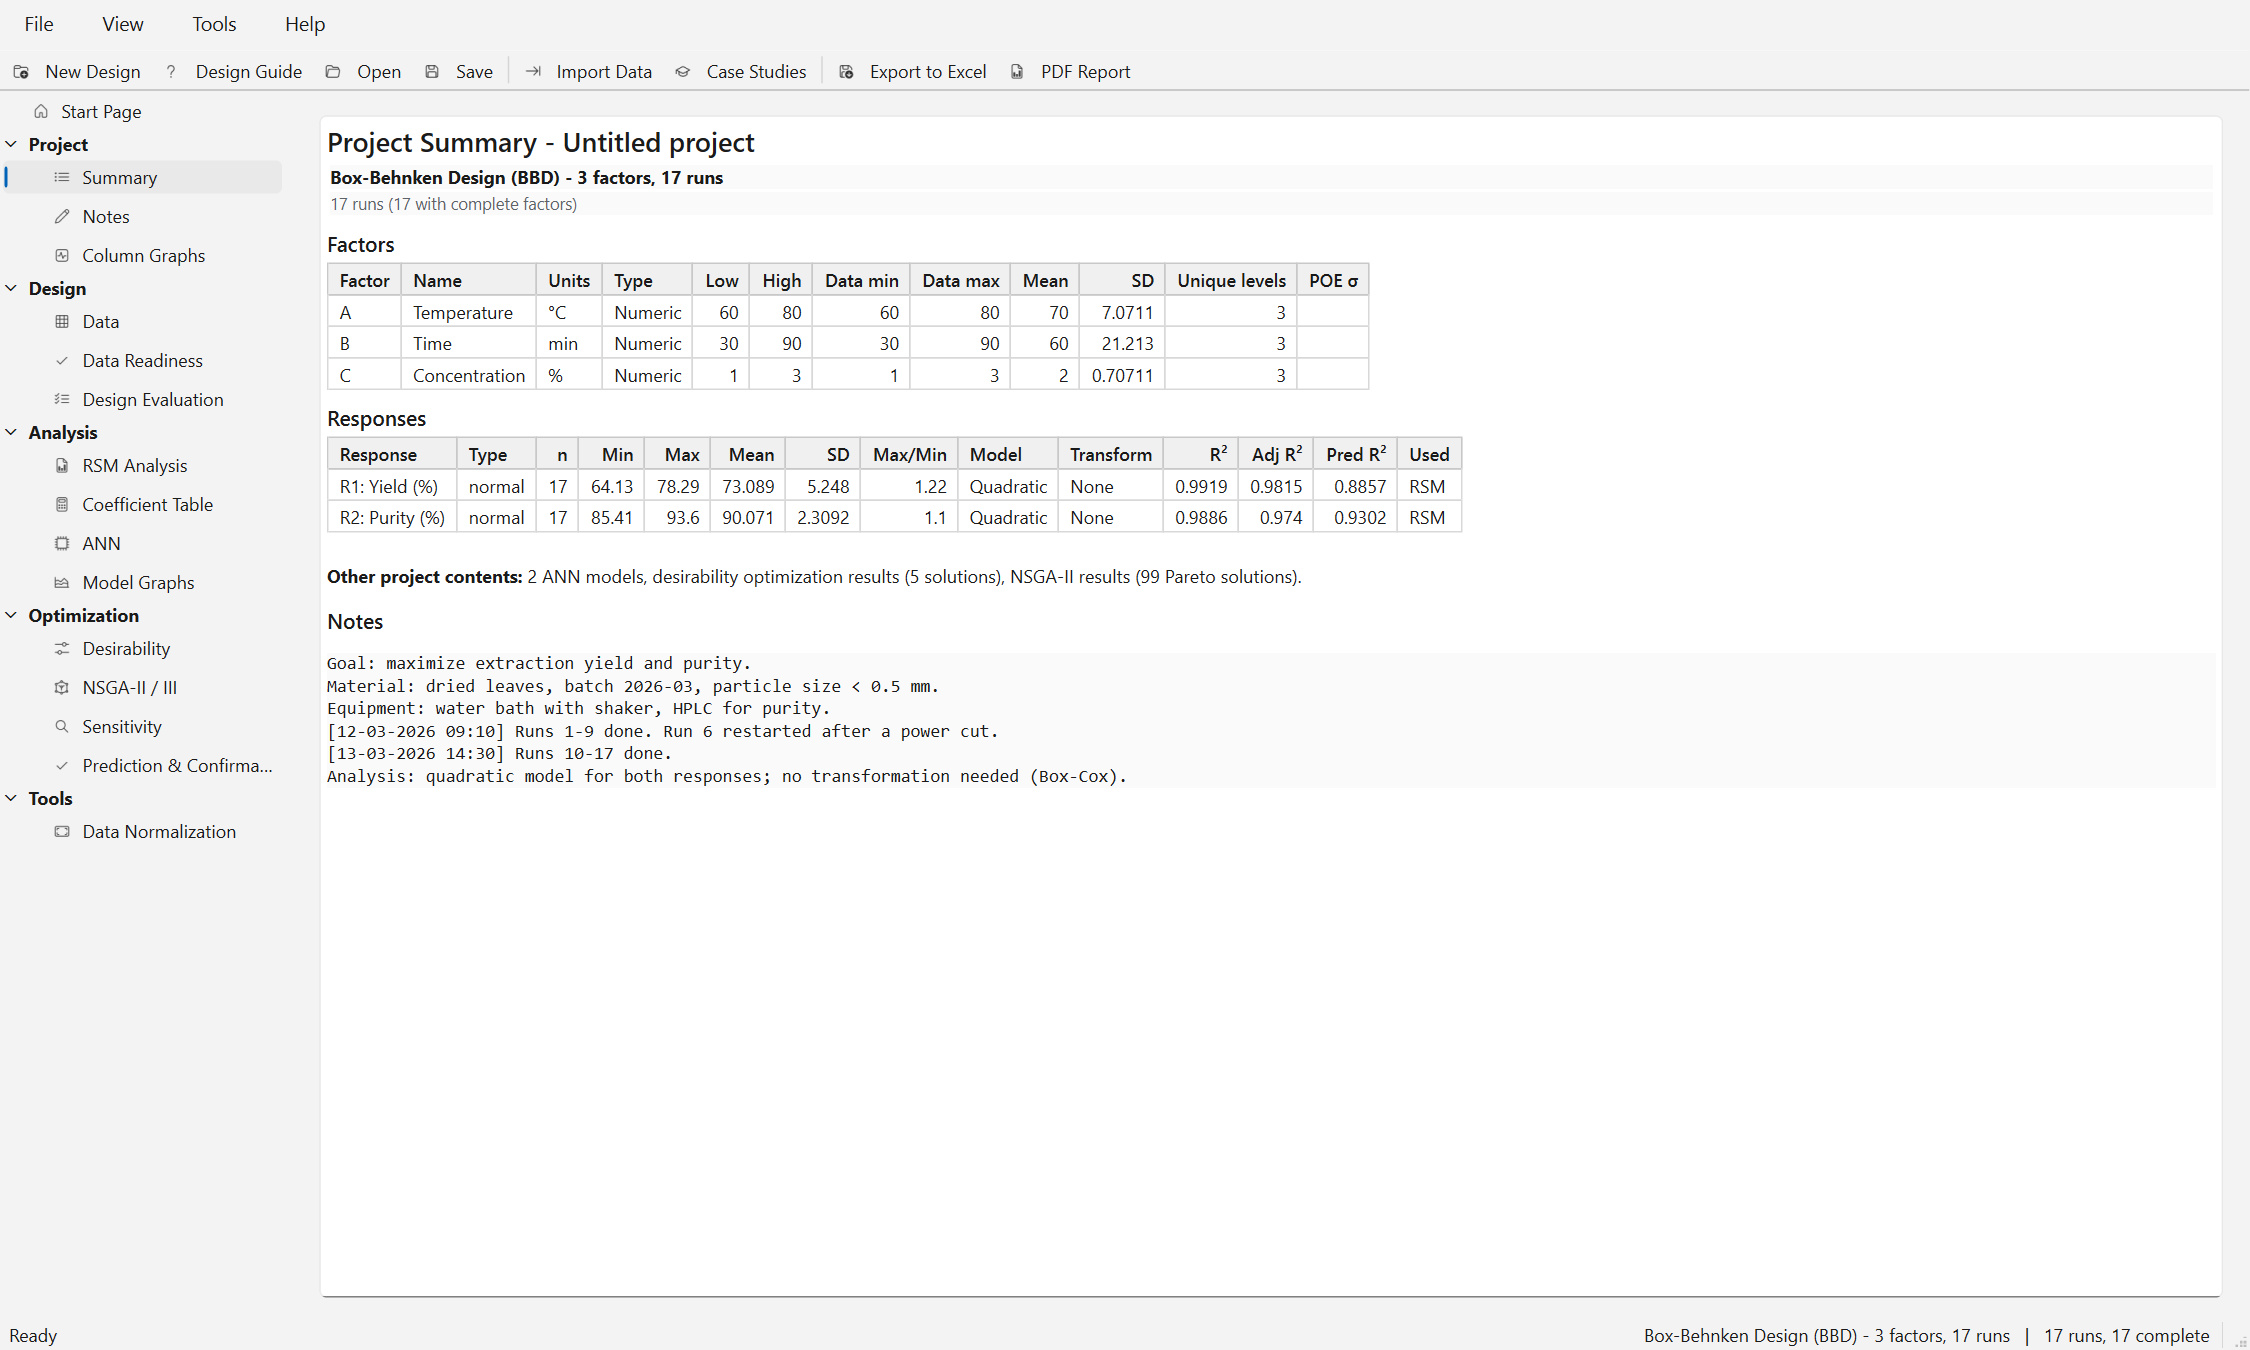
\includegraphics[width=\linewidth]{summary.png}
\caption{\ui{Summary} page of the BBD project at the end of the worked example.}
\label{fig:ch11-summary}
\end{figure}

% ======================================================================================================
\section{Checklist for reporting the study (Part A)}
\label{sec:ch11-checklist}
\begin{table}[htbp]
\centering
\small
\caption{What to report, with the values of the BBD example.}
\label{tab:ch11-checklist}
\begin{tabularx}{\linewidth}{@{}>{\raggedright\arraybackslash}p{2.6cm} >{\raggedright\arraybackslash}X@{}}
\toprule
Item & BBD extraction example \\
\midrule
Design and data & Box-Behnken, 3 factors, 17 runs, 5 center points; readiness \ui{Ready} (94/96 and 100/97). \\
Models & Quadratic RSM; Yield $R^2$ 0.992, predicted $R^2$ 0.886, lack of fit $p=0.030$ (pure error 4 df); Purity $R^2$
0.989, predicted $R^2$ 0.930. \\
Check A & ANN 3-4-1 and 3-5-1 selected by 5-fold CV, $Q^2$ 0.624 and 0.774 (RSM on the same folds 0.598 and 0.818). \\
Check B & ``Too little data to assess''; RSM more accurate at 17 runs. \\
Desirability & Limits 75--78.29 and 89--93.6, importance equal, linear shape; $D=0.862$ at 70.3~°C, 89.8~min,
1.80~\%. \\
NSGA & NSGA-II, population 100, seed 1, automatic stop at generation 78, 99 solutions; TOPSIS 71.5~°C, 88.2~min,
1.88~\%. \\
Check C & Converged (gain $-0.029$~\% $<$ 0.10~\%); population sufficient (seed spread 0.02~\%, 2$\times$ population
+0.35~\%). \\
Check D & Failed: $\Delta=22.4$~\% (Yield), $dx=56$~\%; RSM retained, confirmation at both TOPSIS points. \\
Sensitivity & Sobol $S_T$: Temperature 0.60 / 0.71, Time 0.36 / 0.17, Concentration 0.08 / 0.15 (Yield / Purity). \\
Confirmation & PI (95~\%, $n=3$): Yield 76.9--79.7, Purity 91.7--93.2 at the optimum; Yield 72.1--75.8 at the ANN TOPSIS
point. \\
\bottomrule
\end{tabularx}
\end{table}

% ======================================================================================================
\section{Part C: multi-objective optimization of a polygeneration plant}
\label{sec:ch11-polygen}
Part C follows a complete multi-objective study. The case \ui{Polygeneration Plant (3 Objectives)} contains 80 runs of
an illustrative thermodynamic and thermoeconomic model of a plant that uses geothermal heat to produce power (organic
Rankine cycle), cooling (absorption chiller) and fresh water (reverse osmosis). The runs are simulated with a Latin
hypercube and a small random noise; they are not measurements of a real plant, but they behave the way such a study
does in practice: a plant model is evaluated at space-filling points, a surrogate model is fitted, and the surrogate
is optimized. The five decision variables and the three objectives are:
\begin{itemize}
  \item A: Geothermal Temperature 160--220~°C; B: Turbine Inlet Pressure 1000--2000~kPa; C: Pinch Point 5--15~°C;
        D: RO Recovery Ratio 0.35--0.75; E: Reinjection Temperature 50--90~°C;
  \item Exergy Efficiency (\%, maximize), Product Cost (USD/GJ, minimize), Environmental Impact (mPts/h, minimize).
\end{itemize}
The goals are preset by the case. The settings are the defaults unless stated (ANN seed 1, NSGA seed 1, one CPU core).

\subsection{Readiness}
\ui{Data Readiness} (reference model Quadratic, 21 parameters) rates all three responses \ui{Ready}: modeling scores 92,
92 and 92, optimization scores 91, 94 and 91. The structure is sound (80 complete runs, residual df 59, 79 to 80
distinct levels per factor, maximum VIF 1.63, largest gap in the factor space 0.29), and there are no outliers. Two
items need attention: there are no replicates (pure error df 0, \ui{Problem}), so the noise level and the lack of fit
cannot be assessed, and six runs have high leverage. Without replicates the honest statement is that the surrogate
reproduces the plant model, not that the noise is known; for a simulated data set this is acceptable.

The readiness report also locates the model optimum of each response, and these already show the conflict: the
highest Exergy Efficiency lies at A~=~219.6~°C, B~=~1901~kPa, C~=~5.1~°C, D~=~0.352, E~=~50.8~°C, the lowest Product
Cost at A~=~218.8~°C, E~=~52.0~°C, but the lowest Environmental Impact at A~=~160.9~°C, B~=~1192~kPa, E~=~83.3~°C, at
the other end of the temperature range.

\subsection{Response surface models}
On \ui{RSM Analysis}, \ui{Fit Summary} suggests the quadratic model for all three responses (Exergy Efficiency:
adjusted $R^2$ 0.9947, predicted $R^2$ 0.9923; Product Cost: 0.9767 and 0.9672; Environmental Impact: 0.9924 and
0.9901). The cubic model has a lower predicted $R^2$ for every response (0.9651, 0.9202 and 0.9453), a sign of
overfitting. All five main effects are significant for Exergy Efficiency (model $F=743.5$) and Environmental Impact
($F=516.5$); for Product Cost the linear term of the RO Recovery Ratio is not ($p=0.070$), although its quadratic term
is part of the model. Among the interactions, Geothermal Temperature $\times$ Reinjection Temperature (AE) is significant
for Exergy Efficiency and Geothermal Temperature $\times$ Turbine Inlet Pressure (AB) for Environmental Impact
($p=0.0035$).

\subsection{ANN with checks A and B}
Even with excellent RSM models, the ANN checks are worth running, because check~D needs the networks. On \ui{ANN} the
\ui{Data Adequacy} verdict is \ui{Adequate for ANN modeling} for all three responses. \ui{Optimize All Responses (One
Click)} (check~A) selects:
\begin{itemize}
  \item Exergy Efficiency: 5-3-1 (22 weights), $Q^2=0.9904$; RSM on the same folds 0.9924;
  \item Product Cost: 5-8-4-1 (89 weights), $Q^2=0.9548$; RSM 0.9623;
  \item Environmental Impact: 5-4-1 (29 weights), $Q^2=0.9875$; RSM 0.9892.
\end{itemize}
All three networks are \ui{Good fit}, and each search ends with \ui{RSM predicts new data as well as or better than
ANN (assessed on the same test data)}. The learning curves (check~B) agree: with the full data the ANN reaches a test
$R^2$ of 0.984, 0.964 and 0.984 against 0.991, 0.970 and 0.989 for the RSM (\ui{RSM is more accurate at this data
size}). For Exergy Efficiency and Product Cost the curve is still rising (\ui{More data would still help}), with a run
estimate that the page itself marks as unreliable; for Environmental Impact \ui{The data is sufficient}.

\textbf{Decision.} The RSM models stay selected. The response is smooth, the quadratic surface captures it, and the
networks bring no gain. This is the opposite of the turning case of Chapter~\ref{chap:8}, and it is a normal outcome:
an ANN is justified only when it predicts new data better.

\subsection{NSGA-III and check C}
On \ui{NSGA-II / III} the three goals are already set. The first run with all defaults (population 100, max
generations 300) chooses NSGA-III with 91 reference points and runs all 300 generations. Check~C is not passed: the
quick assessment reads \ui{Not enough generations yet: the mean hypervolume of the last 20 generations is still rising
-0.203\% and the ideal point shifted 1.83\%.} (the hypervolume itself no longer rises; it is the ideal point, the best
value of each objective, that still moves by more than 1~\%), and it adds that all 100 individuals are on the first
front. Raising \ui{Max generations:} to 600 does not help: after 600 generations the ideal point still shifts by
2.19~\%. \ui{Check Population Size} shows where the problem lies: two other seeds change the hypervolume by $+0.27$~\%
and $+1.07$~\%, and a population of 200 adds 3.24~\% and converges after 145 generations, whereas all three runs with
100 individuals use the full 300 generations. The verdict is \ui{Generations: not sufficient, increase the maximum
generations.} and \ui{Population: not sufficient (the result changes by 1.1\% when the seed is changed; a 2x population
increases the hypervolume by 3.2\%). Increase the population, for example to 200, then check again.} A population of
100 is too small to hold the ends of this three-objective front with five decision variables, so the extremes of the
front keep moving.

With \ui{Population:} 200 (190 reference points) the run stops automatically at generation 145 with 197 Pareto
solutions: \ui{Enough generations: the mean hypervolume of the last 20 generations changed by only +0.045\% compared
with the previous 20 generations (limit 0.19\%) and the ideal point shifted 0.16\% (limit 1\%).} The result line is
\ui{NSGA-III: 197 Pareto solutions, automatic stop at generation 145. Best compromise (TOPSIS): Geothermal Temperature =
218.51, Turbine Inlet Pressure = 1401.3, Pinch Point = 10.665, RO Recovery Ratio = 0.74987, Reinjection Temperature =
50.589 $\rightarrow$ Exergy Efficiency = 20.132, Product Cost = 18.194, Environmental Impact = 3.9337}.

\ui{Check Population Size} for this run (Table~\ref{tab:ch11-poly-popcheck}) reports \ui{Generations: sufficient (the
hypervolume has flattened).} but \ui{Population: not sufficient (the result changes by 1.2\% when the seed is changed; a
2x population increases the hypervolume by 1.4\%). Increase the population, for example to 400, then check again.} Both
values are only slightly above the 1~\% limit. A run with population 400 (378 reference points) stops at generation
115 with 389 solutions, and its own population check is passed: \ui{Population: sufficient. Another seed changes the
hypervolume by only 0.66\% and a 2x population adds only 0.98\%.}

\begin{table}[htbp]
\centering
\small
\caption{\ui{Adequacy Check Results} for the polygeneration case (NSGA-III, RSM models, seed 1) with population 200 and
400.}
\label{tab:ch11-poly-popcheck}
\begin{tabular}{@{}lrrlrrrr@{}}
\toprule
Run & Pop. & Seed & Generations & Solutions & HV & Diff. & TOPSIS shift (\%) \\
\midrule
Current result & 200 & 1 & 145 (converged) & 197 & 58.90\% & +0.00\% & 0.0 \\
Different seed & 200 & 102 & 300 & 196 & 58.79\% & $-0.19$\% & 13.5 \\
Different seed 2 & 200 & 203 & 120 (converged) & 190 & 58.21\% & $-1.17$\% & 5.5 \\
Population 2x & 400 & 1 & 115 (converged) & 389 & 59.73\% & +1.40\% & 13.7 \\
\midrule
Current result & 400 & 1 & 115 (converged) & 389 & 58.71\% & +0.00\% & 0.0 \\
Different seed & 400 & 102 & 130 (converged) & 392 & 58.33\% & $-0.65$\% & 7.7 \\
Different seed 2 & 400 & 203 & 110 (converged) & 391 & 58.44\% & $-0.46$\% & 5.4 \\
Population 2x & 800 & 1 & 100 (converged) & 781 & 59.29\% & +0.99\% & 3.7 \\
\bottomrule
\end{tabular}
\end{table}

How much does this matter for the decision? The TOPSIS choice of the population-400 run is 216.04~°C, 1372.4~kPa,
12.031~°C, 0.750, 50.002~°C with Exergy Efficiency 19.59~\%, Product Cost 18.00~USD/GJ and Environmental Impact
3.848~mPts/h. Compared with the population-200 choice, only the Pinch Point moves noticeably (12.0 against 10.7~°C,
13.7~\% of its range), and the objectives change by 0.54 percentage points of efficiency, 0.19~USD/GJ and
0.085~mPts/h, small against the ranges of the front. The front is flat in the Pinch Point direction: a slightly larger
pinch trades a little efficiency for a little cost and impact. The rest of this part uses the population-200 run,
which is the one shown in the screenshots; with population 400 the conclusions are the same. In a report, state the
population that passed check~C (400) and the run used for the figures.

\begin{figure}[htbp]
\centering
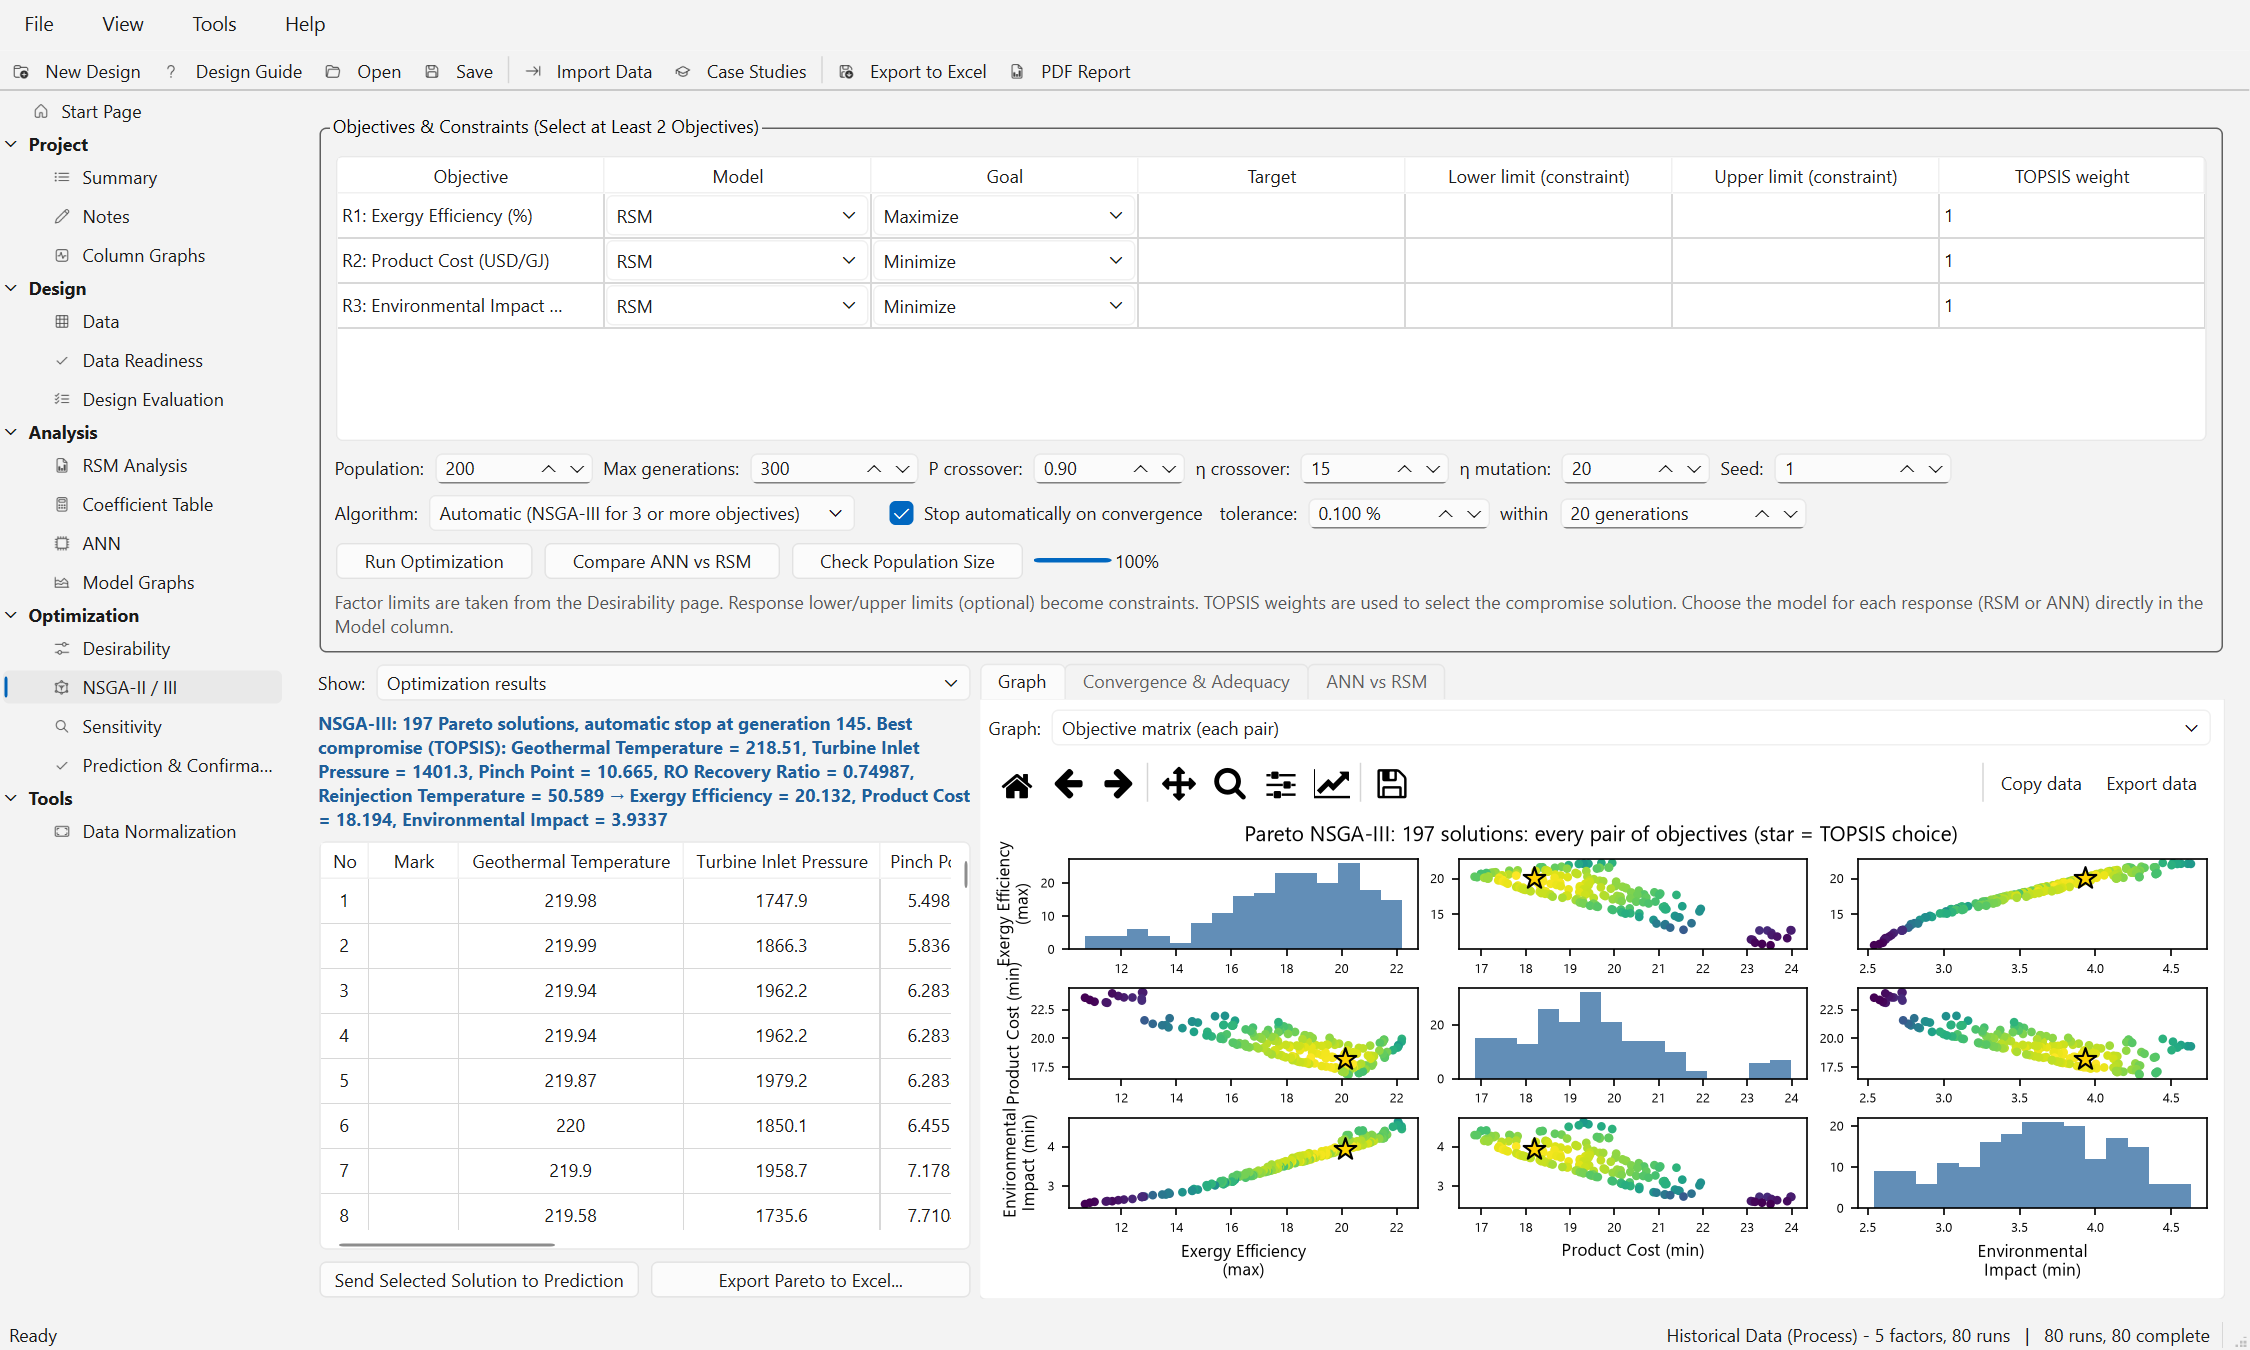
\includegraphics[width=\linewidth]{moo_polygen_front.png}
\caption{NSGA-III front of the polygeneration case (population 200, 197 solutions), \ui{Objective matrix (each pair)}.
Exergy Efficiency and Environmental Impact rise together (conflict), Exergy Efficiency and Product Cost improve
together; the star is the TOPSIS choice.}
\label{fig:ch11-poly-front}
\end{figure}

The objective matrix (Figure~\ref{fig:ch11-poly-front}) shows the shape of the front: Exergy Efficiency ranges from
10.68 to 22.19~\%, Product Cost from 16.85 to 24.00~USD/GJ and Environmental Impact from 2.54 to 4.63~mPts/h.
Efficiency and impact rise together along an almost straight band, while the cost falls as the efficiency rises.

\subsection{Check D: ANN versus RSM}
\ui{Compare ANN vs RSM} with the same settings (population 200, seed 1) gives the green verdict \ui{Both models agree:
predictions on the front differ by only 3.0\% on average and the compromise choices are close together. The
optimization result does not depend on the choice of model.} The details:
\begin{itemize}
  \item fronts of 197 (RSM, 145 generations) and 198 solutions (ANN, 100 generations); hypervolume 58.7~\% and
        58.3~\% by the own model, 57.3~\% and 58.1~\% by the other model;
  \item mean (maximum) prediction difference on the fronts: Exergy Efficiency 1.9~\% (7.2~\%), Product Cost 3.0~\%
        (10.8~\%), Environmental Impact 1.6~\% (5.4~\%) of the data range;
  \item TOPSIS choices: RSM front 218.51~°C, 1401.3~kPa, 10.665~°C, 0.7499, 50.589~°C (Exergy Efficiency 20.132 by RSM
        and 20.151 by ANN, Product Cost 18.194 and 18.047, Environmental Impact 3.9337 and 3.9691); ANN front
        216.24~°C, 1412.6~kPa, 12.063~°C, 0.7499, 50.011~°C (19.738 and 19.793, 17.929 and 17.852, 3.8768 and
        3.9191). The distance is $dx=14.0$~\%, just inside the 15~\% limit, and it comes from the Pinch Point (10.7
        against 12.1~°C): the front is flat in that direction;
  \item accuracy on new data: RSM mean predicted $R^2$ 0.983, ANN mean cross-validation $Q^2$ 0.978.
\end{itemize}
Check~D is passed. Together with checks A and B it says that the result does not depend on the surrogate: two
different model families, fitted to the same 80 runs, lead to the same trade-off and to compromise settings whose
predicted objectives differ by less than 0.4~percentage points of efficiency.

\subsection{Sensitivity and parametric study}
On \ui{Sensitivity} choose \ui{Start from:} \ui{NSGA: TOPSIS choice} and \ui{Model:} \ui{Selected model of each
response}. The results are discussed in Section~\ref{sec:ch09-polygen} of Chapter~\ref{chap:9}
(Figures~\ref{fig:ch09-poly-param}--\ref{fig:ch09-poly-front}); in short:
\begin{itemize}
  \item the Geothermal Temperature sets the trade-off: it has the largest standardized coefficient for all three
        objectives ($+0.727$, $-0.582$, $+0.844$) and the largest Sobol index for efficiency (0.465) and impact
        (0.604), and it changes steadily along the front ($\rho=0.95$ with efficiency);
  \item the Pinch Point is the second lever for the cost (Sobol $S_T=0.365$), the Turbine Inlet Pressure for the
        impact (0.202);
  \item Reinjection Temperature and RO Recovery Ratio stay near one of their bounds on most of the front (about
        50~°C and 0.75): they can be fixed there;
  \item the responses are almost additive (sum of $S_1$ at least 0.996).
\end{itemize}
\ui{Local Sensitivity (Tornado)} with $\pm10$~\% adds the view from the chosen point: the Exergy Efficiency (20.132)
changes most with the Turbine Inlet Pressure (19.764 at 1301~kPa, 20.433 at 1501~kPa) and the Geothermal Temperature
(19.623 at 212.5~°C, 20.258 at 220~°C), and the Product Cost (18.194) most with the Pinch Point (18.492 at 9.66~°C,
17.957 at 11.66~°C). In the plant these are the variables to control most tightly around the chosen setting.

\subsection{Choice of the compromise}
The front offers a continuum of designs, and the choice depends on how much the environmental impact weighs against
efficiency and cost. Two candidates are marked on the page:
\begin{itemize}
  \item TOPSIS (equal weights): 218.51~°C, 1401.3~kPa, 10.665~°C, 0.7499, 50.589~°C with Exergy Efficiency 20.13~\%,
        Product Cost 18.19~USD/GJ and Environmental Impact 3.934~mPts/h;
  \item knee point: 201.34~°C, 1424.3~kPa, 13.618~°C, 0.7475, 50.128~°C with Exergy Efficiency 18.20~\%, Product
        Cost 18.45~USD/GJ and Environmental Impact 3.619~mPts/h.
\end{itemize}
Moving from the TOPSIS choice to the knee lowers the impact by 8~\% (3.934 to 3.619) and costs 1.93 percentage points
of efficiency and 0.26~USD/GJ. Both lie in the interior of the front, away from its ends (efficiency 10.7 and
22.2~\%), where the models are least supported by data. In this example the TOPSIS choice is taken as the design point,
and the knee is kept as the low-impact alternative. Other preferences are expressed with the \ui{TOPSIS weight}
column, or by a response limit, for example an \ui{Upper limit (constraint)} on the Environmental Impact.

\subsection{Confirmation plan}
\ui{Send Selected Solution to Prediction} (without a selection the TOPSIS solution is sent) gives the predictions with
their intervals. Because the runs come from a deterministic plant model, ``confirmation'' here means one new evaluation
of the plant model at the chosen point, so set \ui{Number of confirmation runs (n):} to 1. The 95~\% prediction
intervals for a single run are then:
\begin{itemize}
  \item TOPSIS point: Exergy Efficiency 19.74--20.53~\%, Product Cost 17.61--18.78~USD/GJ, Environmental Impact
        3.848--4.019~mPts/h;
  \item knee point: 17.79--18.62~\%, 17.83--19.08~USD/GJ, 3.528--3.710~mPts/h.
\end{itemize}
With the default $n=3$ (for repeated measurements on a real plant or pilot unit) the intervals at the TOPSIS point are
19.82--20.44~\%, 17.73--18.66~USD/GJ and 3.866--4.001~mPts/h. Evaluate the plant model at both points; if the values
fall inside the intervals, the surrogate is confirmed where it matters. Because the data have no replicates, the
residual variance behind these intervals contains the small lack of fit of the quadratic models as well as the noise,
so they are, if anything, slightly conservative. If a value falls outside, add the evaluated point to the data, refit
and repeat the optimization.

\subsection{Export of the data}
For a report or paper the following exports cover the study:
\begin{itemize}
  \item \ui{Export Pareto to Excel\dots} on the NSGA page: the 197 solutions with factor values, all responses and the
        TOPSIS score (sheet \texttt{Pareto}), the settings and the stop reason (\texttt{Settings}), the convergence
        history (\texttt{Convergence}) and, after check~D, the sheets \texttt{RSM Front}, \texttt{ANN Front} and
        \texttt{ANN vs RSM};
  \item the reports of check~C (\ui{Convergence \& Adequacy}) and check~D (\ui{ANN vs RSM}) with \ui{Export all
        tables\dots};
  \item the significance table, the Sobol tables, the tornado tables and the Spearman tables of the
        \ui{Sensitivity} page with \ui{Export all tables\dots}, and the data behind every graph (for example the
        parametric curves) with \ui{Export data\dots};
  \item the ANOVA tables and fit summaries of the three RSM models, and the architecture search tables of the ANN
        page;
  \item the whole project with \menupath{File $\rightarrow$ Export to Excel\dots} and \menupath{File $\rightarrow$
        PDF Report\dots}.
\end{itemize}

% ======================================================================================================
\section{Part C, mixture variant: concrete mix paste}
\label{sec:ch11-concrete}
The case \ui{Concrete Mix Paste (Mixture, 3 Objectives)} shows the same workflow for a constrained mixture: cement
(45--75~\%), fly ash (0--30~\%) and water (20--35~\%) of the paste, with the water/binder ratio limited to 0.35--0.60
by two linear constraints, 14 runs of a D-optimal design and quadratic Scheff\'e models (predicted $R^2$ 0.993, 0.984
and 0.997). Compressive Strength is maximized, Material Cost and CO2 Emission are minimized. Two things differ from a
process study. First, the factors are not independent: NSGA-III works on the simplex and repairs every new blend so
that the components sum to 100~\%, and the constraints are handled as violations
(Section~\ref{sec:ch08-nsga} of Chapter~\ref{chap:8}). Second, the Sobol indices are not available for a pure mixture,
because mixture components cannot vary one at a time; the trade-off is read from the front and the ternary graphs.

With the defaults NSGA-III stops at generation 120 with 92 solutions (Figure~\ref{fig:ch11-concrete-front}). The front
runs from 32.5 to 52.7~MPa, 84.9 to 99.8~USD/t and 425 to 661~kg/t of CO2. Up to 45.9~MPa the cement content stays at
its minimum of 45--45.6~\%, and the strength is gained by replacing water with fly ash (fly ash 20 to 29~\%, water 35 to
26~\%); the CO2 emission stays between 425 and 432~kg/t while the cost rises. Beyond that point more cement is the only
way to more strength, and the CO2 jumps to 478~kg/t at 46.2~MPa and above 600~kg/t from about 48.5~MPa. The TOPSIS
choice sits exactly at this step:
cement 45.0~\%, fly ash 29.0~\%, water 26.0~\% with 45.89~MPa, 94.27~USD/t and 428.4~kg/t. The desirability
optimization with the preset goals (limits = data range) finds a neighbouring blend, cement 45~\%, fly ash 27.8~\%,
water 27.2~\% ($D=0.626$), shown in the ternary desirability contour (Figure~\ref{fig:ch11-concrete-desir}).

\begin{figure}[htbp]
\centering
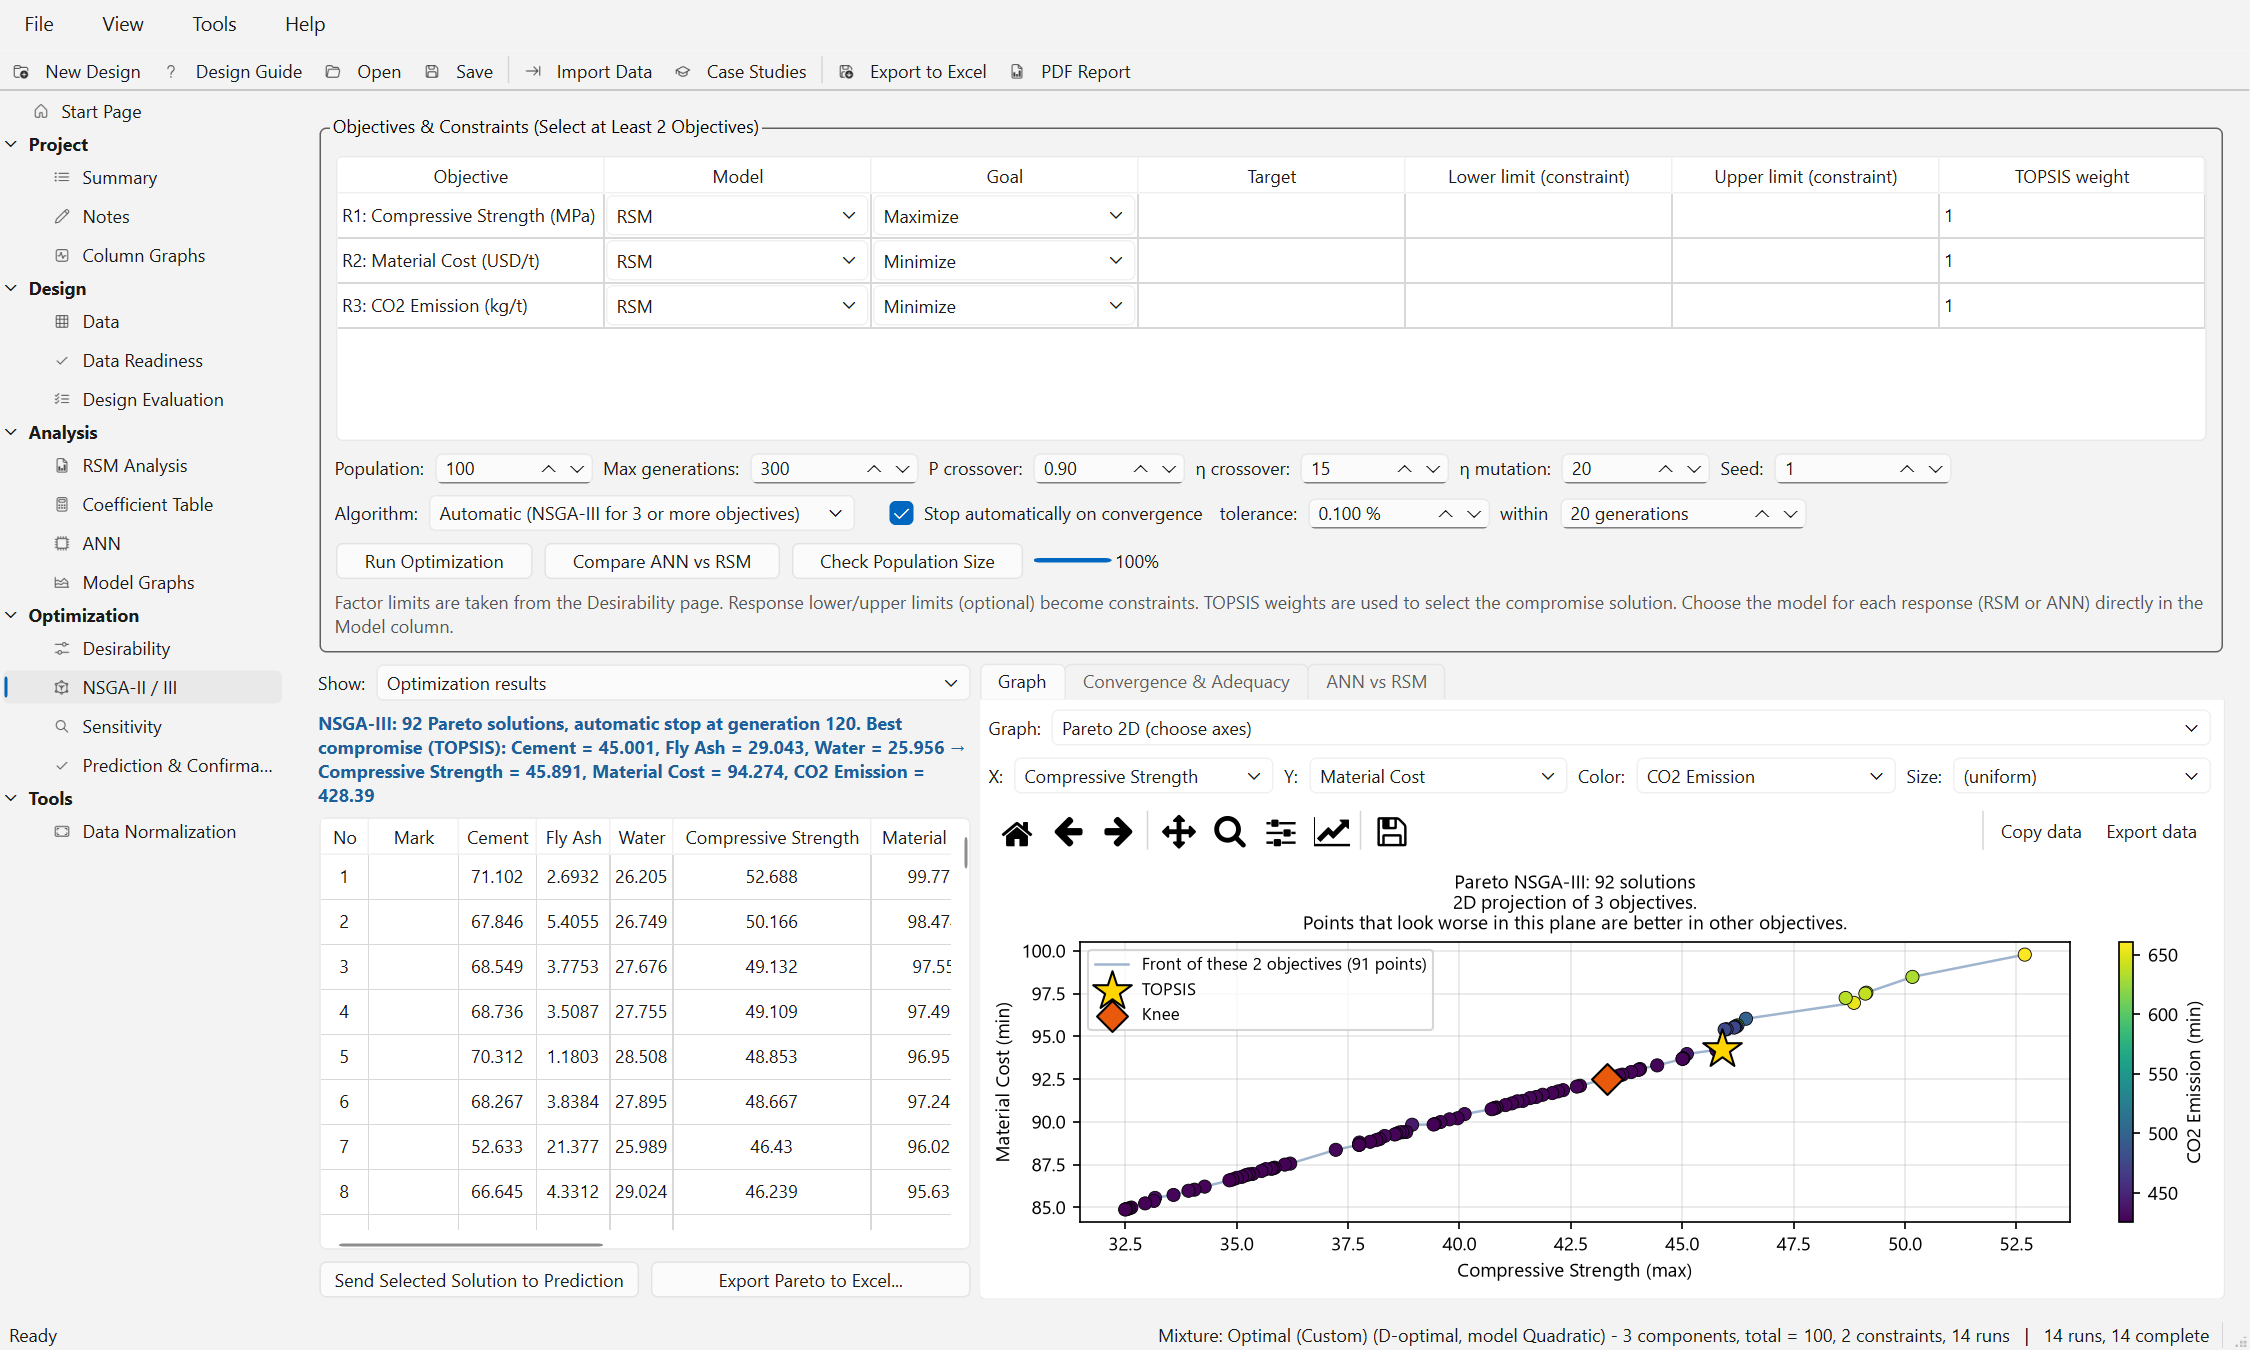
\includegraphics[width=\linewidth]{moo_concrete_front.png}
\caption{NSGA-III front of the concrete mix paste, \ui{Pareto 2D (choose axes)}: Compressive Strength against Material
Cost, colored by CO2 Emission. Beyond about 46~MPa the emission jumps (yellow points).}
\label{fig:ch11-concrete-front}
\end{figure}

\begin{figure}[htbp]
\centering
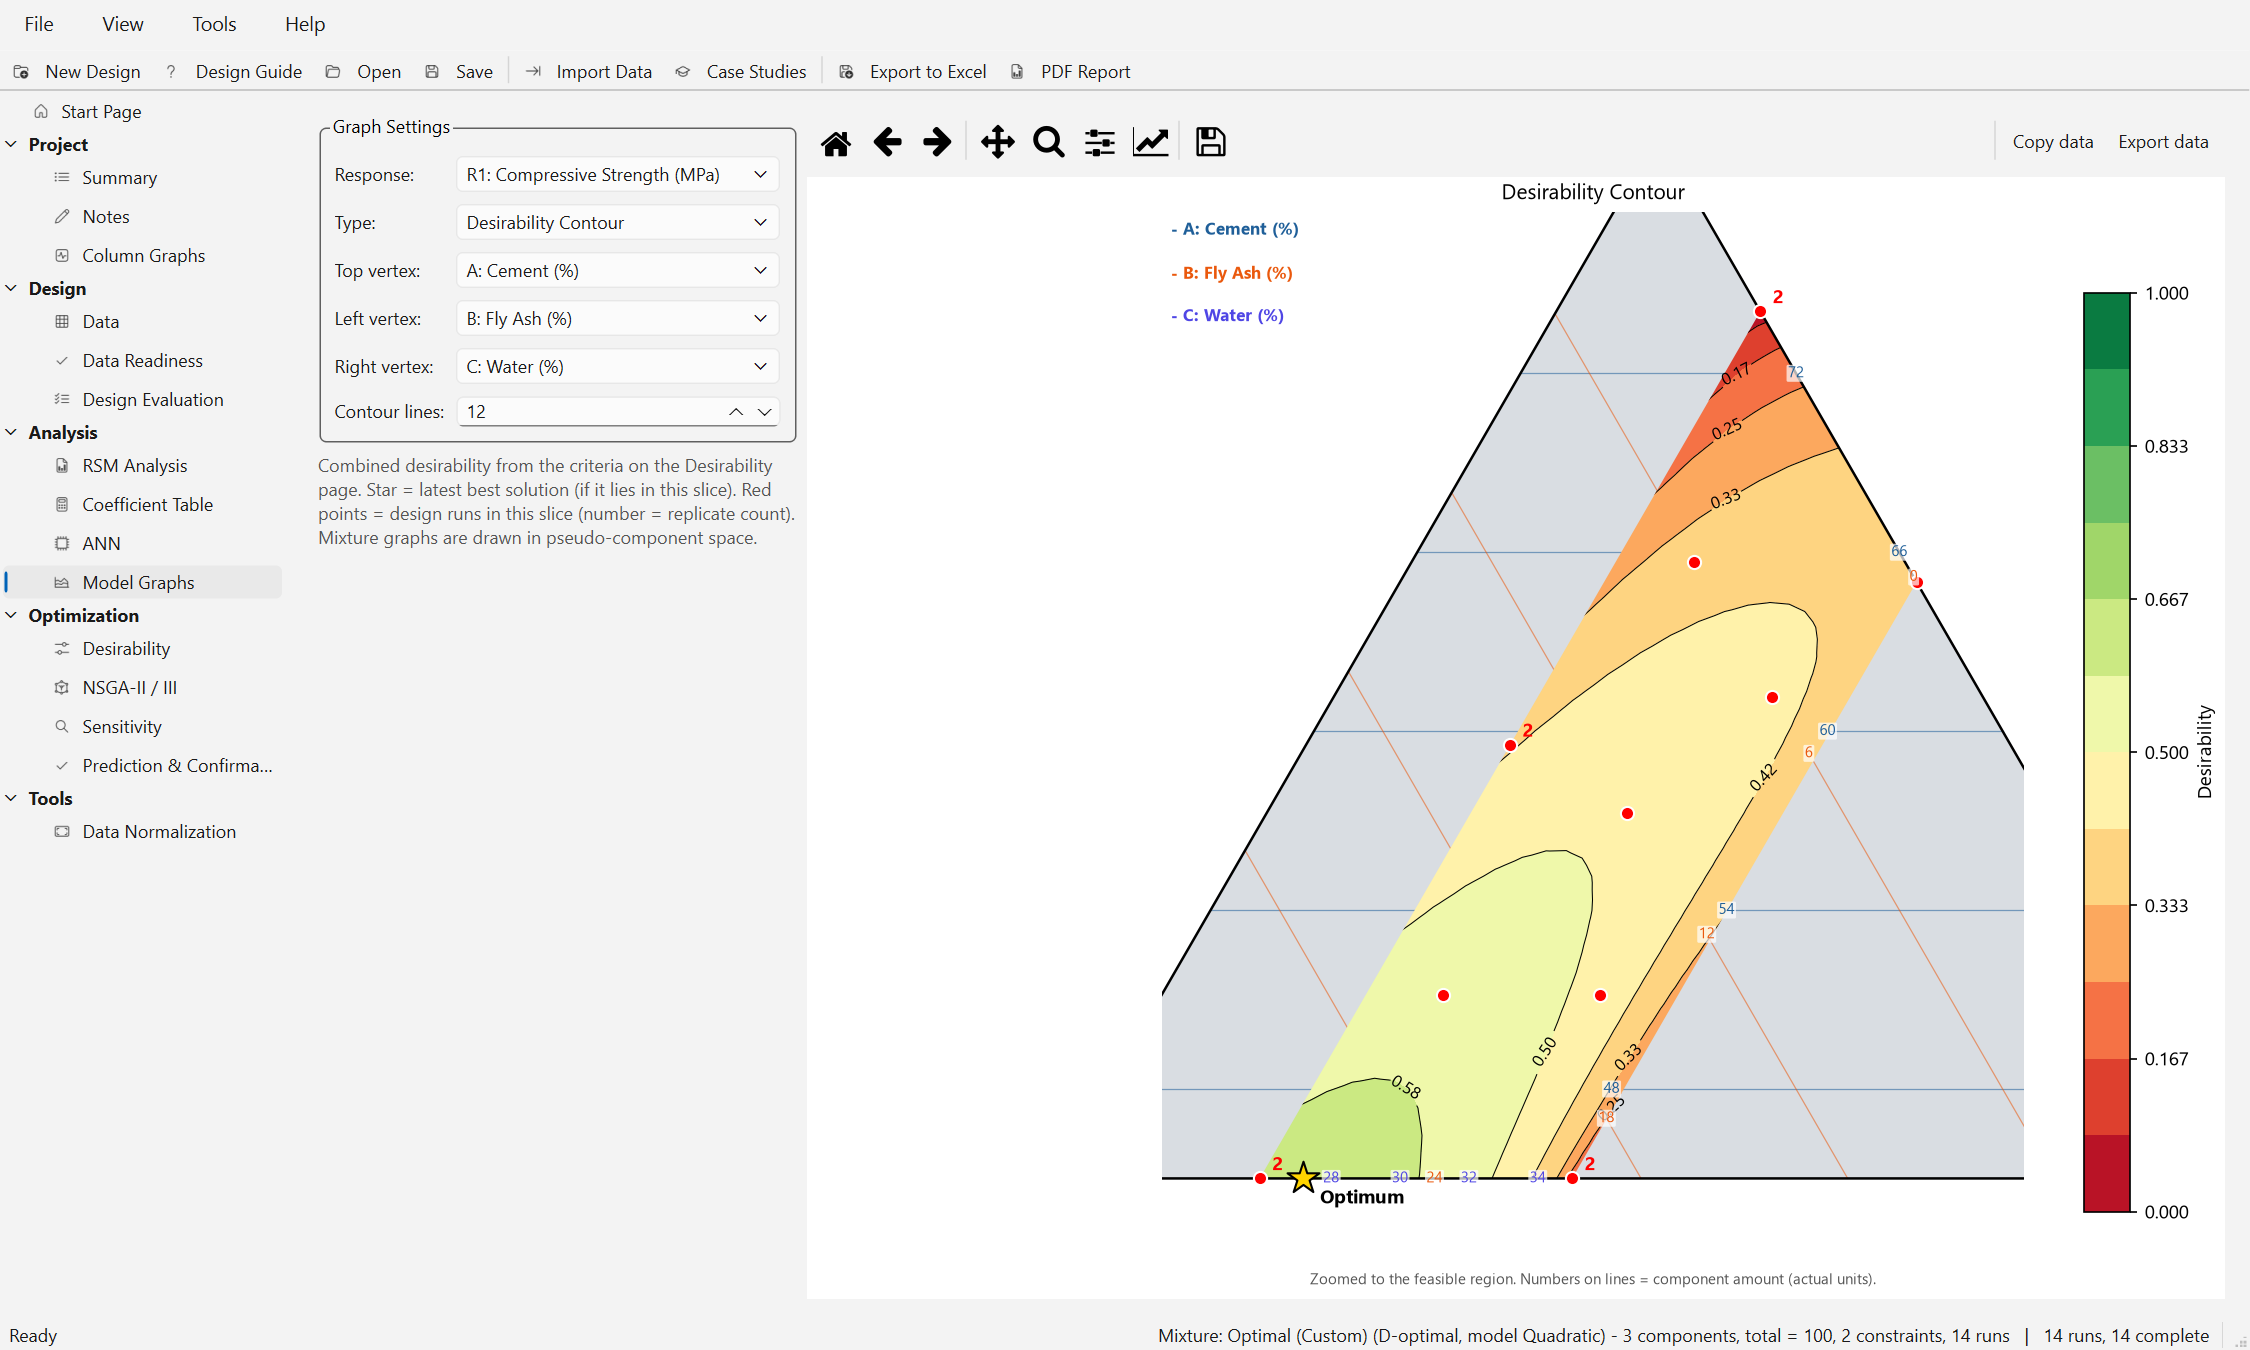
\includegraphics[width=\linewidth]{moo_concrete_desirability.png}
\caption{\ui{Desirability Contour} of the concrete mix paste in the constrained ternary region (pseudo-components,
zoomed to the feasible band between the two water/binder constraints); the star marks the best desirability blend.}
\label{fig:ch11-concrete-desir}
\end{figure}

% ======================================================================================================
\section{Checklist for the multi-objective study}
\label{sec:ch11-checklist-moo}
\begin{table}[htbp]
\centering
\small
\caption{What to report, with the values of the polygeneration example (Part C).}
\label{tab:ch11-checklist-moo}
\begin{tabularx}{\linewidth}{@{}>{\raggedright\arraybackslash}p{2.6cm} >{\raggedright\arraybackslash}X@{}}
\toprule
Item & Polygeneration plant example \\
\midrule
Data & 80 simulated runs (Latin hypercube) of an illustrative plant model, 5 decision variables; readiness \ui{Ready}
(modeling 92/92/92, optimization 91/94/91); no replicates. \\
Models & Quadratic RSM, predicted $R^2$ 0.992, 0.967, 0.990 (efficiency, cost, impact). \\
Check A & ANN 5-3-1, 5-8-4-1, 5-4-1; $Q^2$ 0.990, 0.955, 0.988 against RSM 0.992, 0.962, 0.989 on the same folds;
RSM kept. \\
Check B & ANN test $R^2$ 0.984, 0.964, 0.984 against RSM 0.991, 0.970, 0.989 with the full data. \\
NSGA & NSGA-III, population 200 (100 did not converge), seed 1, automatic stop at generation 145, 197 solutions. \\
Check C & Population 100: not converged after 300 (or 600) generations. Population 200: converged at generation 145
(gain +0.045~\% $<$ 0.19~\%, ideal point shift 0.16~\%), population check slightly above the limits (1.2~\%, 1.4~\%).
Population 400: converged at 115, population check passed (0.66~\%, 0.98~\%); TOPSIS objectives within 0.54 points of
efficiency of the population-200 choice. \\
Check D & Passed: $\Delta=3.0$~\% (cost), $dx=14.0$~\%. \\
Sensitivity & Geothermal Temperature dominant ($\beta$ $+0.73$/$-0.58$/$+0.84$; Sobol $S_T$ 0.47/0.36/0.60); sum of
$S_1\ge0.996$. \\
Compromise & TOPSIS 218.5~°C, 1401~kPa, 10.7~°C, 0.750, 50.6~°C: 20.13~\%, 18.19~USD/GJ, 3.934~mPts/h; knee as
low-impact alternative. \\
Confirmation & One plant-model evaluation; PI (95~\%, $n=1$) 19.74--20.53~\%, 17.61--18.78~USD/GJ, 3.848--4.019~mPts/h. \\
\bottomrule
\end{tabularx}
\end{table}

\chapter{Troubleshooting and Frequently Asked Questions}\label{chap:12}
\label{ch:trouble}

This chapter collects the messages that REGEN can show, explains why they appear and what to do. Messages are
quoted as the program shows them; parts in angle brackets (such as $\langle$name$\rangle$) are filled in with the
actual factor, response or number. The last sections answer common questions about reproducibility, speed and
installation.

\section{Installation, starting and files}
\label{sec:ch12-files}

{\small\begin{longtable}{@{}p{0.38\linewidth}p{0.58\linewidth}@{}}
\caption{Installation and file messages.}\label{tab:ch12-files}\\
\toprule
Message or problem & Cause and what to do \\
\midrule
\endfirsthead
\toprule
Message or problem & Cause and what to do \\
\midrule
\endhead
\bottomrule
\endfoot
``Windows protected your PC'' when the installer starts &
Windows SmartScreen warns about a downloaded program that is not code-signed. Check that the file is the REGEN
installer from the GitHub Releases page, click \ui{More info} and then \ui{Run anyway}
(Section~\ref{sec:ch02-install}). \\
\addlinespace
The installer asks for administrator rights &
\ui{Install for all users} was chosen. Choose \ui{Install for me only}, which needs no administrator rights. \\
\addlinespace
Double-clicking a \texttt{.doe} file does not open REGEN &
The file association was not selected during installation. Run the installer again and tick \ui{Open .doe files
with REGEN}, or open the file with \menupath{File $\rightarrow$ Open\dots}. \\
\addlinespace
``Open Failed: The file could not be opened: $\langle$error$\rangle$'' &
The file is not a REGEN/DOE Studio project, it was damaged (for example cut off while copying, or edited by hand
and no longer valid JSON), or it is locked by another program. Open a backup copy; the error text names the
problem (for example the line of a JSON error). \\
\addlinespace
``Save Failed: $\langle$error$\rangle$'' &
The folder is read-only, the disk is full, or the file is open in another program (for example a cloud-sync
client). Save to another folder with \ui{Save As\dots}. \\
\addlinespace
``Export Failed'' / ``PDF Export Failed'' &
The target file is open in another program (an Excel workbook or PDF viewer keeps the file locked) or the folder is
not writable. Close the file or choose another name. \\
\addlinespace
``Export data: The file could not be written: $\langle$error$\rangle$'' &
Same as above, for \ui{Export data\dots}, \ui{Export table\dots} and \ui{Export all tables\dots}. \\
\addlinespace
``Export data: There are no data to export.'' &
The plot or panel is empty (for example a message is shown instead of a plot). \\
\addlinespace
A project opens without the last NSGA result or search table &
Results larger than 5 million characters (for example a very large Pareto history) are not stored in the file, and
projects saved by older versions contain no results. Run the analysis again. \\
\addlinespace
``User Manual: The user manual (REGEN\_User\_Manual.pdf) was not found next to the program\dots'' &
The PDF manual is missing from the installation folder. Reinstall REGEN or download the manual from the Releases
page. \\
\end{longtable}}

\section{New design and import}
\label{sec:ch12-design}

{\small\begin{longtable}{@{}p{0.38\linewidth}p{0.58\linewidth}@{}}
\caption{Messages when creating a design or importing data.}\label{tab:ch12-design}\\
\toprule
Message & Cause and what to do \\
\midrule
\endfirsthead
\toprule
Message & Cause and what to do \\
\midrule
\endhead
\bottomrule
\endfoot
``Factor $\langle$name$\rangle$: Low must be less than High.'' / ``The limits of $\langle$name$\rangle$ are not
numbers.'' & Correct the factor table. Decimal comma and point are both accepted. \\
\addlinespace
``The sum of the component lower limits must be less than the total.'' &
In a mixture the lower limits must leave room for the components to vary: $\sum L_i < T$. Lower some limits or
raise the mixture total. \\
\addlinespace
``Categorical factor $\langle$name$\rangle$ needs at least 2 distinct levels.'' &
Separate the level names with semicolons (or commas), for example \texttt{Ethanol; Methanol}. \\
\addlinespace
``Constraint: Line $\langle i\rangle$: A constraint must use <= or >=.'' and similar &
A linear constraint could not be read. Write one constraint per line with factor letters, numbers and \texttt{<=}
or \texttt{>=}, for example \texttt{A + B <= 160} or \texttt{2A - C >= 0}. Constraints may not contain categoric
factors, and only letters of existing factors (``Factor 'X' does not exist (use letters A–C).''). \\
\addlinespace
``The design region is empty: the bounds and constraints contradict each other.'' &
No point satisfies all limits and constraints at the same time. Relax a constraint or widen a factor range. \\
\addlinespace
``There are not enough candidate points to estimate this model. Relax the constraints or choose a simpler model.'' &
Optimal designs choose runs from a candidate set; in a small constrained region the set cannot support all model
coefficients. Use a lower-order planned model or relax the constraints. \\
\addlinespace
``Box-Behnken requires at least 3 factors.'', ``DSD is available for 3–20 factors.'', ``PB with $N$ runs allows at
most $N-1$ factors.'', ``$\langle$array$\rangle$ allows at most $m$ factors.'' &
The chosen design type does not exist for this number of factors. Choose another type or size (the Design Guide
lists the valid choices). \\
\addlinespace
``Split-plot: Enter the letters of the hard-to-change factors (e.g. A).'' &
The split-plot option is ticked but no hard-to-change factor is given. \\
\addlinespace
\ui{Augment Design\dots} is greyed out; tooltip ``Augmenting split-plot designs is not supported: the new runs would
need their own whole plots. Create a new split-plot design instead.'' &
Split-plot designs cannot be augmented. Create a larger split-plot design, or add runs suggested by Data Readiness
(each new run becomes its own whole plot). \\
\addlinespace
``Import: The clipboard is empty. Copy a data table first.'' &
Nothing was copied, or the copied content is not text. Copy the cells again in Excel. \\
\addlinespace
``Mark at least one Factor column and one Response column.'' &
Set the column roles by right-clicking the column headers (Section~\ref{sec:ch02-import}). \\
\addlinespace
``Factor $\langle$name$\rangle$ is constant / empty - mark it as Ignore.'' &
A factor must take at least two different values. Constant columns carry no information for a model. \\
\addlinespace
``Column $\langle$name$\rangle$, row $i$ is not a number: '$\langle$value$\rangle$'.'' &
A cell of a numeric column contains text (such as ``n/a'' or a unit). Delete the row, clear the cell before
copying, or mark the column as categoric. Cells shown in red are the ones that will fail. \\
\addlinespace
``$\langle$name$\rangle$ has $L$ levels - should this column be numeric or ignored?'' &
A text column with more than 20 different values was marked as a categoric factor. It is probably an identifier
(mark it \ui{Ignore}) or a numeric column with some text cells. \\
\addlinespace
``Mixture components cannot be combined with process factors when importing data.\dots'' &
An import is either a process or a mixture data set. Mark all factor columns as components, or none. \\
\addlinespace
``In $n$ rows the components do not sum to the total $T$. Continue (those rows are still analyzed)?'' &
Check \ui{Mixture total}; it is set to the median row sum. Small rounding differences are harmless; large ones
indicate a wrong column or a wrong total. \\
\addlinespace
``Sum of component minimums ≥ total - check the mixture total.'' &
The lower limits taken from the data leave no room for variation. Check the total and the component columns. \\
\addlinespace
Numbers such as 1,234 are read as 1.234 &
A comma alone is read as a decimal comma. Remove thousands separators before copying. \\
\end{longtable}}

\section{Data, analysis and graphs}
\label{sec:ch12-analysis}

{\small\begin{longtable}{@{}p{0.38\linewidth}p{0.58\linewidth}@{}}
\caption{Messages on the data, analysis and graph pages.}\label{tab:ch12-analysis}\\
\toprule
Message & Cause and what to do \\
\midrule
\endfirsthead
\toprule
Message & Cause and what to do \\
\midrule
\endhead
\bottomrule
\endfoot
``The model cannot be computed yet'' with ``Fill in at least 3 complete rows (factors + response) to start the
analysis.'' & The response has fewer than 3 runs with complete factor settings and a response value (excluded runs
do not count). Enter more data. \\
\addlinespace
``Residual degrees of freedom = 0 (saturated model). Statistical tests cannot be computed - remove model terms or
add runs.'' &
The model has as many coefficients as there are runs, so no error estimate exists. Choose a lower-order model,
remove terms, or add runs (Data Readiness suggests D-optimal runs). Design Evaluation shows the degrees of freedom
before any run is made. \\
\addlinespace
``Aliased terms (removed automatically): $\langle$terms$\rangle$'' &
These terms cannot be estimated separately from terms earlier in the model (for example a cubic term in a
Box-Behnken design, or interactions in a resolution III fraction). They are dropped from the model; the Fit Summary
marks such orders ``Aliased''. Use a design of higher resolution, add runs (augmentation, foldover) or use a
lower-order model. \\
\addlinespace
``No model is significant compared with the mean.'' &
None of the model orders explains the response better than its mean (sequential $p \ge 0.05$). The factors may
have no effect in the studied range, the noise may be large, or the ranges may be too narrow. \\
\addlinespace
``The square root transform requires all response values ≥ 0.'' / ``The $\langle$transform$\rangle$ transform
requires all response values > 0.'' &
Set \ui{Constant k (y + k)} so that $y+k$ is positive, or choose another transformation. \\
\addlinespace
``The Box-Cox plot needs all values of y + k > 0 (and at least 3 data points).'' / ``Box-Cox is not available for
this response.'' &
Box-Cox needs positive values and is only available for ordinary least squares (not for logistic, Poisson or
split-plot models). \\
\addlinespace
``No effect exceeds the ME limit.'' &
Lenth's automatic selection found no effect larger than the margin of error. Inspect the half-normal plot; select
terms by clicking if there is a clear break. \\
\addlinespace
``The GLM fit has warnings - see the GLM (Logistic/Poisson) tab.'' &
The IRLS fit did not converge, or fitted probabilities are numerically 0 or 1 (complete or quasi-complete
separation; for Poisson: fitted means 0). Standard errors, tests and odds ratios are then not reliable. Remove terms
or add runs where the response changes. \\
\addlinespace
``A binomial response must be a number of successes between 0 and $m$ (number of trials).'' / ``A Poisson
response (counts) cannot be negative.'' &
Check the response type and \ui{Trials per run} in \ui{Factor \& Response Info\dots}, and the data. \\
\addlinespace
``Whole-plot df = 0: hard-to-change factor effects cannot be tested properly. Add more whole plots (replicates).'' &
In a split-plot design the hard-to-change factors are tested against the whole plots. With too few whole plots no
test is possible. \\
\addlinespace
``This slice lies entirely outside the design region. Change the values of the other factors/components.'' &
With the values chosen in \ui{Other Factor Values} (or \ui{Other Components}), no point of the plotted slice
satisfies the constraints or component bounds. Move the other factors toward the center of the region. \\
\addlinespace
``This graph needs more numeric factors.'' &
The graph type needs two (contour, surface, overlay) or three (cube) numeric factors. \\
\addlinespace
``No criteria yet. Choose response goals and limits on the Desirability page.'' &
Overlay and desirability contours use the goals of the Desirability page. Set at least one goal there. \\
\addlinespace
``Enter the factor standard deviations first (Data page $\rightarrow$ Factor \& Response Info\dots).'' &
Propagation of error needs the standard deviation of at least one factor. \\
\addlinespace
``No complete runs to evaluate yet.'' (Design Evaluation) &
All runs have missing factor settings or are excluded. \\
\addlinespace
``Simulation: Invalid equation: \dots'' / ``Unknown name 'x'.\dots'' &
Use the factor letters (A, B, \dots), \texttt{+ - * / **} (or \texttt{\^{}}), and the listed functions; use a point
as decimal separator inside an equation (commas separate the arguments of \texttt{min} and \texttt{max}). \\
\end{longtable}}

\section{Artificial neural networks}
\label{sec:ch12-ann}

{\small\begin{longtable}{@{}p{0.38\linewidth}p{0.58\linewidth}@{}}
\caption{Messages on the ANN page.}\label{tab:ch12-ann}\\
\toprule
Message & Cause and what to do \\
\midrule
\endfirsthead
\toprule
Message & Cause and what to do \\
\midrule
\endhead
\bottomrule
\endfoot
``ANN here is for continuous (normal) responses. For binomial/Poisson responses use logistic/Poisson regression on
the RSM Analysis page.'' & ANN models are trained only for normal responses. \\
\addlinespace
``Too little data to train an ANN (at least 4 complete runs required).'' / ``Too little training data. Increase the
training data percentage.'' & Enter more data or change \ui{Training data:} so that the training set is not empty. \\
\addlinespace
``Training + validation + test percentages must add up to 100\%.'' & Adjust the three percentages. \\
\addlinespace
``Early stopping requires validation data (> 0\%).'' &
Set \ui{Validation data:} above 0, or untick early stopping. \\
\addlinespace
``Enter the neurons per hidden layer as numbers separated by commas. Example: 20, 10, 5'' &
One number per hidden layer; each layer needs at least 1 neuron. \\
\addlinespace
``Constant response - the ANN cannot be trained.'' &
All training values are equal; there is nothing to learn. \\
\addlinespace
``Only $N$ complete runs. Architecture search needs at least 8 runs.'' &
Cross-validation needs enough runs to form folds. Use a fixed architecture or RSM. \\
\addlinespace
``The learning curve needs at least 12 complete runs (found $N$).'' &
With fewer runs no learning curve can be estimated. \\
\addlinespace
Learning curve: ``Too little data ($N$ runs) for a reliable learning curve.'' &
The curve was computed but $N<25$, so its extrapolation is not trusted. An ANN generally needs at least 20 to 30
runs; use RSM. \\
\addlinespace
Learning curve: ``(run estimate unreliable)'' &
The fitted power law reached the edge of the exponent range (0.2 to 2.5), its error limit is 0, or the
interquartile range of the run estimate is very wide (upper/lower above 3). Use the curve only to decide whether
more runs help, not how many. \\
\addlinespace
Status ``Overfitting'' or ``Underfitting'' &
Overfitting: the error on new data is far above the training error; use fewer neurons, Bayesian regularization,
or more data. Underfitting: even the training error is high; use more neurons or check the data. After an
architecture search the headline status comes from cross-validation; the single train/test split of the final
model is shown separately and is less reliable with few runs. \\
\addlinespace
Negative ANN or RSM test $R^2$ &
With few runs a test set of 2--3 runs gives a meaningless $R^2$. Use the cross-validated $Q^2$ of the
architecture search. A negative RSM cross-validation $R^2$ for Box-Behnken or CCD data is explained in the report:
leaving runs out destroys the design structure; compare with the RSM predicted $R^2$. \\
\addlinespace
``The search was stopped before finishing; the results above are from the architectures evaluated so far.'' &
\ui{Stop} was clicked. The table and the selection use only the finished candidates. \\
\addlinespace
``Architecture $\langle$layers$\rangle$ is too large for the computer's memory; adding neurons was stopped.'' /
``A parallel process stopped unexpectedly (possibly not enough memory).'' &
Reduce \ui{CPU cores (parallel):}, set a maximum number of neurons, or close other programs. \\
\addlinespace
``Large data ($N$ runs): the search uses 4000 random runs for speed; the final model is trained on all data.'' &
Information only. \\
\end{longtable}}

\section{Optimization, sensitivity and prediction}
\label{sec:ch12-opt}

{\small\begin{longtable}{@{}p{0.38\linewidth}p{0.58\linewidth}@{}}
\caption{Messages on the optimization, sensitivity and prediction pages.}\label{tab:ch12-opt}\\
\toprule
Message & Cause and what to do \\
\midrule
\endfirsthead
\toprule
Message & Cause and what to do \\
\midrule
\endhead
\bottomrule
\endfoot
``Choose a goal (Maximize/Minimize/Target/In range) for at least one response whose model is available.'' &
All response goals are \ui{None}, or the responses with a goal have no model yet. Set a goal in the
\ui{Goal} column. \\
\addlinespace
``Skipped responses without a model: $\langle$names$\rangle$'' &
These responses have a goal but no model (not enough data, or ANN chosen but not trained). The optimization runs
without them. \\
\addlinespace
``Limits for response $\langle$name$\rangle$: lower must be < upper.'' / ``The target for $\langle$name$\rangle$
must be between the limits.'' & Correct the limits in the criteria table. \ui{Reset Limits to Data} restores the
data minimum and maximum. \\
\addlinespace
``No point satisfies all limits and constraints.'' / ``The component limits do not allow the mixture to sum to the
total.'' &
The factor limits on the Desirability page, the component bounds and the constraints leave no feasible point. Widen
the factor limits. \\
\addlinespace
Desirability $D = 0$ for all solutions &
At least one response cannot reach its lower limit (maximize) or upper limit (minimize) anywhere in the region.
Relax that limit; the bar chart of a solution shows which individual $d_i$ is 0. \\
\addlinespace
``Select at least 2 objectives (maximize/minimize/target).'' / ``NSGA-II requires at least 2 objectives\dots'' &
NSGA-II/III builds a Pareto front between two or more objectives. For one objective use the Desirability page. A
row with goal \ui{Ignore} but with limits counts only as a constraint. \\
\addlinespace
``Enter a target value for $\langle$name$\rangle$.'' & Goal \ui{Target} needs a value in the \ui{Target} column. \\
\addlinespace
``The model for $\langle$name$\rangle$ is not available yet.'' & Fit the RSM model or train the ANN for that
response first. \\
\addlinespace
``No feasible solution. Relax the response limits or constraints.'' &
No solution of the final population satisfies the response limits. Widen the limits or remove some. \\
\addlinespace
``There is no ANN model for the objective responses yet. Train an ANN first on the ANN page (Optimize All Responses
button).'' & \ui{Compare ANN vs RSM} needs an ANN for the objectives. \\
\addlinespace
``Run the optimization first.'' & \ui{Check Population Size} and \ui{Send Selected Solution to Prediction} need a
result. \\
\addlinespace
``Automatic stop was not used: with NSGA-II and 4 or more objectives\dots'' &
For NSGA-II with four or more objectives the automatic stop is switched off and all generations are run. Use
NSGA-III (or \ui{Automatic}) for a reliable automatic stop. \\
\addlinespace
``Not enough generations yet\dots'' / ``Population: not sufficient\dots'' &
Check C was not passed. Increase \ui{Max generations:} or \ui{Population:} and run again
(Table~\ref{tab:ch01-checks}). \\
\addlinespace
``The models differ considerably\dots'' (red) &
Check D: the RSM and ANN fronts disagree. Make confirmation runs at both TOPSIS points and trust the model with the
better predictive accuracy. \\
\addlinespace
``Sobol indices need at least one process or categoric factor. Mixture components sum to a constant and are not
independent inputs.'' &
Sobol indices, standardized coefficients and the tornado chart vary independent factors only. In a pure mixture use
the parametric study, the trace plot or the Pareto trade-off instead. \\
\addlinespace
``The linear constraints of the design are not applied here\dots'' &
Sobol indices assume independent factors, so they describe the whole factor box, including points outside the
constraints. \\
\addlinespace
``Too few points of the sample satisfy the design constraints.'' &
The constrained region is too small a part of the factor box for the Latin hypercube sample. Increase
\ui{Sample size:}. \\
\addlinespace
``Reference point: The reference point lies outside the design region (component bounds or constraints).\dots'' &
Change the reference values or choose another start for the sensitivity study. \\
\addlinespace
``Run NSGA-II / NSGA-III on the multi-objective optimization page first.'' & The Pareto trade-off analysis needs an
NSGA result. \\
\addlinespace
``The point is outside the design region - the prediction is an extrapolation.'' &
A factor is set beyond the range of the design and of the data. Predictions there are not supported by data. \\
\addlinespace
``This point violates the component bounds / constraints.'' / ``The component sum does not equal the mixture
total.'' & Correct the prediction point. \\
\addlinespace
Prediction shows ``-'' for the standard error, CI and PI &
The response uses an ANN, which gives only a point prediction. Confirmation is then judged by the error as a
percentage of the response data range (at most 5\,\%). \\
\end{longtable}}

\section{Frequently asked questions}
\label{sec:ch12-faq}

\paragraph{Why do I get a different run order every time I create the same design?}
The run order (and the choice of points in optimal, Latin hypercube and hybrid designs) is random. The
\ui{Random seed:} in the New Design dialog controls it: the same seed gives the same design. A new random seed is
proposed every time the dialog opens; type a fixed number to reproduce a design. The seed is saved with the project
and shown on the Summary page and in the PDF report.

\paragraph{Are the results reproducible?}
Yes. Every random step has a seed: the design seed, \ui{Random seed:} on the ANN page (data split, initial weights,
cross-validation folds), \ui{Seed:} on the NSGA-II / III page, and fixed internal seeds for the desirability
search, the region samples of Data Readiness and Design Evaluation, and the sensitivity samples. With the same data,
settings and seeds the same numbers are obtained. ANN results do not depend on the number of CPU cores.

\paragraph{The ANN gives a different result each time I click Train ANN.}
This happens only when settings change between clicks (data, split percentages, seed, algorithm). Keep the seed
fixed; to see how much the result depends on the initialization, change only the seed.

\paragraph{The calculation is slow. What can I do?}
For ANN work increase \ui{CPU cores (parallel):} (the default already uses all cores but one), reduce
\ui{Restarts (initializations):} or \ui{Maximum epochs:}, or limit the number of neurons and layers of the
architecture search. With more than 5000 runs the number of restarts of the final training is limited
automatically, and with more than 4000 runs the architecture search uses a random subset of 4000 runs. For
NSGA-II/III keep \ui{Stop automatically on convergence} on. For RSM, data sets with more than 400 runs are handled
with a faster algorithm automatically; data sets with 15\,000 runs have been tested.

\paragraph{The computer becomes slow while REGEN trains networks.}
Reduce \ui{CPU cores (parallel):}. The worker processes close by themselves 90 seconds after the last calculation.

\paragraph{Can I use REGEN without administrator rights?}
Yes: choose \ui{Install for me only} during installation.

\paragraph{Where is the list of recent projects stored?}
In the Windows user settings (registry) under the old program name ``DOE Studio'', so the list of earlier versions
is kept. Deleted or moved files are not shown.

\paragraph{Can I change the factor ranges of an existing design?}
The factor settings of a designed experiment are fixed once the design is created (the data sheet shows them in
grey). For historical data (created with Import Data or the Historical Data design types) the factor cells can be
edited on the Data page.

\paragraph{How do I remove an outlier without deleting it?}
Select the run on the Data page and click \ui{Exclude/Restore Runs}, or select the point on the diagnostics plots
and click \ui{Exclude Selected Runs}. Excluded runs are left out of all models, Design Evaluation and Data
Normalization, but stay in the data sheet and in the exports (marked ``Excluded'') and can be restored at any time.


\appendix
\chapter{Reference}
\label{ch:reference}

This appendix collects reference material: keyboard and mouse shortcuts, the structure of the project file, the
constants and thresholds used by the computations, and a glossary of the terms used in this manual.

\section{Keyboard and mouse shortcuts}
\label{sec:a-keys}

\begin{table}[htbp]
\centering
\caption{Keyboard and mouse shortcuts.}
\label{tab:a-keys}
\small
\begin{tabularx}{\linewidth}{@{}lX@{}}
\toprule
Shortcut & Action \\
\midrule
Ctrl+N & \menupath{File $\rightarrow$ New Design\dots} \\
Ctrl+O & \menupath{File $\rightarrow$ Open\dots} \\
Ctrl+S & \menupath{File $\rightarrow$ Save} \\
Ctrl+Shift+S & \menupath{File $\rightarrow$ Save As\dots} \\
Alt+F4 & \menupath{File $\rightarrow$ Exit} (close REGEN) \\
F1 & \menupath{Help $\rightarrow$ User Manual} \\
Alt+F, Alt+V, Alt+T, Alt+H & Open the File, View, Tools or Help menu (then the underlined letter of an item) \\
\addlinespace
Ctrl+C & Copy the selected cells of a table (data sheet and result tables) as tab-separated text \\
Ctrl+V & Data sheet: paste a block of cells copied from Excel, starting at the current cell (cells beyond the table
  are ignored; decimal comma or point) \\
Delete, Backspace & Data sheet: clear the selected editable cells \\
\addlinespace
Click a point & Diagnostics plots: identify the run (the same run is highlighted in all plots); half-normal and
  normal effects plots: add the term to or remove it from the model \\
Ctrl+click, Shift+click & Diagnostics plots: add a point to or remove it from the selection \\
Double-click a row & Diagnostics report table: highlight the run in the plots \\
Right-click & Plots: \ui{Copy plot data}, \ui{Export plot data\dots}; tables: copy and \ui{Export table\dots};
  report panels: \ui{Copy all tables (for Excel)}, \ui{Export all tables\dots}; Import dialog: column roles (on a
  header) and \ui{Delete $n$ Selected Rows} (on cells) \\
Double-click & Start Page: open a recent project; Case Studies: open the case; Design Guide: create the selected
  design \\
\bottomrule
\end{tabularx}
\end{table}

\section{Project file format}
\label{sec:a-file}

A project file (\texttt{*.doe}) is a UTF-8 text file in JSON format, written with indentation so that it can be
inspected in a text editor. Table~\ref{tab:a-file} lists the top-level fields of the current format (field
\texttt{version} = 3). Factor settings are stored in coded units (pseudo-components for mixture components, level
indices for categoric factors); actual values are recomputed from the factor ranges. Missing values are stored as
\texttt{null}. Rows of \texttt{coded}, \texttt{data}, \texttt{point\_types}, \texttt{blocks} and
\texttt{run\_order} are in standard order (the order in which the design was created; Std = row number).

{\small\begin{longtable}{@{}p{0.2\linewidth}p{0.76\linewidth}@{}}
\caption{Top-level fields of a \texttt{.doe} project file.}\label{tab:a-file}\\
\toprule
Field & Content \\
\midrule
\endfirsthead
\toprule
Field & Content \\
\midrule
\endhead
\bottomrule
\endfoot
\texttt{version} & File format version (3). \\
\texttt{design\_type} & Design type key, for example \texttt{bbd}, \texttt{ccd}, \texttt{full\_factorial},
  \texttt{simplex\_lattice}, \texttt{optimal\_rsm}, \texttt{combined\_optimal}, \texttt{lhs}, \texttt{historical}. \\
\texttt{options} & Design options (center points, alpha, blocks, planned model, random seed, augmentation labels,
  \dots). \\
\texttt{mixture\_total} & Total of the mixture components (1 for process designs). \\
\texttt{factors} & List of factors: \texttt{name}, \texttt{unit}, \texttt{low}, \texttt{high}, \texttt{kind}
  (\texttt{numeric}, \texttt{categoric}, \texttt{process}), \texttt{levels} (categoric level names), \texttt{upper}
  (upper limit of a mixture component), \texttt{sd} (standard deviation for propagation of error). For mixture
  components \texttt{low} is the lower limit. \\
\texttt{responses} & List of responses: \texttt{name}, \texttt{unit}, \texttt{kind} (\texttt{normal},
  \texttt{binomial}, \texttt{poisson}), \texttt{trials} (binomial trials per run). \\
\texttt{coded} & Matrix of factor settings, one row per run, coded units. \\
\texttt{point\_types} & Point type of each run (Factorial, Center, Axial, Edge, Vertex, Historical, \dots). \\
\texttt{blocks} & Block number of each run. \\
\texttt{run\_order} & Run number of each run. \\
\texttt{constraints} & Linear constraints: \texttt{text}, \texttt{coef}, \texttt{op}, \texttt{rhs} (actual
  units). \\
\texttt{groups}, \texttt{htc} & Whole-plot number of each run and indices of the hard-to-change factors
  (split-plot designs; otherwise \texttt{null} and empty). \\
\texttt{data} & Matrix of response values, one row per run, one column per response. \\
\texttt{model\_specs} & Per response (key = response index): \texttt{order}, \texttt{terms} (selected terms as
  exponent vectors, or \texttt{null} for the full model of the order) and \texttt{transform} (kind, $\lambda$,
  constant $k$). \\
\texttt{opt\_criteria} & Desirability criteria: factor limits (keys \texttt{f0}, \texttt{f1}, \dots), response goals,
  limits, target, importance and shape (key = response index), and POE criteria (\texttt{poe0}, \dots). \\
\texttt{ann} & Trained ANN models per response: architecture, activation, weights and biases, normalization
  parameters, data split, seed, metrics and the cross-validated diagnosis. A combined (multi-output) network is
  stored once and referenced by its responses. \\
\texttt{model\_source} & \texttt{rsm} or \texttt{ann} for each response. \\
\texttt{excluded} & Indices of the runs excluded from the analysis. \\
\texttt{notes} & Text of the Notes page. \\
\texttt{results} & Saved results: \texttt{ann\_search}, \texttt{learning}, \texttt{solutions},
  \texttt{criteria\_used}, \texttt{nsga\_result}, \texttt{nsga\_compare}. Numerical arrays are stored as
  \{\texttt{"\_\_array\_\_"}: values, \texttt{"shape"}, \texttt{"dtype"}\}. A result larger than 5\,000\,000
  characters is left out. \\
\end{longtable}}

Older files (DOE Studio, versions 1 to 6) have the same structure without some of the newer fields; missing fields
take default values, and point-type labels of the earliest versions are translated when the file is read. Editing a
project file by hand is possible but not recommended: an invalid file cannot be opened (Chapter~\ref{chap:12}).

\section{Constants and thresholds}
\label{sec:a-constants}

The tables below list the fixed numbers used by the computations: significance levels, limits of diagnostic plots,
algorithm settings and the thresholds of the readiness and adequacy checks. Values that can be changed in the user
interface are marked ``default''. $n$ is the number of runs used in a model, $p$ the number of model coefficients,
$N$ the number of complete runs.

{\small\begin{longtable}{@{}p{0.26\linewidth}p{0.46\linewidth}p{0.22\linewidth}@{}}
\caption{Design and design evaluation.}\label{tab:a-const-design}\\
\toprule
Item & Value & Where used / meaning \\
\midrule
\endfirsthead
\toprule
Item & Value & Where used / meaning \\
\midrule
\endhead
\bottomrule
\endfoot
Factor letters & A--H, J--Z (no I), at most 25 & All pages \\
Rotatable CCD alpha & $\alpha = n_F^{1/4}$ & $n_F$ = number of factorial points \\
Optimal designs: lack-of-fit and replicate points & 5 and 5 (default) & New Design \\
Optimal designs: search & exchange algorithm, 6 random starts, at most 300 iterations; I-criterion averaged over 3000
  region points & New Design \\
Latin hypercube & maximin $\phi_p$ criterion with $p=15$; $\min(20\,000, 200n)$ annealing iterations; random
  (not optimized) above 2000 points & New Design \\
Power in Design Evaluation & $\Delta = 2$, $\sigma = 1$, $\alpha = 0.05$ (defaults); target 80\,\% & Design
  Evaluation, Design Guide \\
VIF & ideal 1; $> 10$ high correlation & Design Evaluation \\
Recommended degrees of freedom & lack of fit $\ge 3$, pure error $\ge 4$, residual $\ge 5$ & Design Evaluation \\
FDS and matrix measures & 4000 and 3000 random points of the region & Design Evaluation \\
G-efficiency & model columns only (no block columns); maximum of $v(x)$ over the design points, the corners or
  vertices of the region (up to 4096 combinations; none above 12 process factors) and the 3000 random points & Design
  Evaluation \\
\end{longtable}}

{\small\begin{longtable}{@{}p{0.26\linewidth}p{0.46\linewidth}p{0.22\linewidth}@{}}
\caption{Data Readiness (status: ok / needs attention / problem).}\label{tab:a-const-ready}\\
\toprule
Check & Thresholds & Meaning \\
\midrule
\endfirsthead
\toprule
Check & Thresholds & Meaning \\
\midrule
\endhead
\bottomrule
\endfoot
Score & ok = 100, needs attention = 50, problem = 0; $\ge 85$ Ready, $\ge 60$ Fair, $< 60$ Not ready yet & Mean of
  the check statuses \\
Runs vs model parameters & residual df $\ge 5$ ok, $\ge 1$ attention, 0 problem & Error estimate \\
Numeric factor levels & $\ge 3$ levels per factor & Needed for curvature \\
Replicates (pure error) & pure-error df $\ge 3$ ok, $\ge 1$ attention, 0 problem & Lack-of-fit test \\
Multicollinearity & max VIF $\le 5$ ok, $\le 10$ attention & \\
High leverage & $h_i > \max(2p/n,\,0.5)$ & \\
Factor space coverage & largest gap $\le 0.3$ ok, $\le 0.5$ attention (relative to the diagonal) & \\
Outliers and influence & Bonferroni limit of the studentized residuals; Cook's distance $> 1$ & \\
Response transform & recommended by Box-Cox and residual SS lower by $\ge 5\,\%$ & \\
Constant variance & Spearman correlation of $|e|$ and $\hat y$ positive with $p < 0.05$ & \\
Drift over run order & Durbin-Watson $< 1.4$ or $> 2.6$, or trend $p < 0.01$ & \\
Model fit & lack of fit $p < 0.05$, Adj $-$ Pred $R^2 > 0.2$ or Pred $R^2 < 0.5$ (attention); Pred $R^2 < 0$
  (problem) & Info for split-plot (REML) responses \\
Signal / noise & $\ge 4$ ok, $\ge 2$ attention & SD of response / pure-error SD \\
Model significance & model $p < 0.05$ & Optimization readiness; Info for split-plot (REML) responses \\
Prediction reliability & Pred $R^2 \ge 0.7$ ok, $\ge 0.4$ attention & \\
Optimum location & within 2\,\% of a factor bound & Optimum at the edge \\
Data support at the optimum & distance to nearest run $> 0.2$ or CI half-width $> 10\,\%$ of the response range &
  Confirmation runs suggested \\
\end{longtable}}

{\small\begin{longtable}{@{}p{0.26\linewidth}p{0.46\linewidth}p{0.22\linewidth}@{}}
\caption{RSM analysis and diagnostics.}\label{tab:a-const-rsm}\\
\toprule
Item & Value & Where used / meaning \\
\midrule
\endfirsthead
\toprule
Item & Value & Where used / meaning \\
\midrule
\endhead
\bottomrule
\endfoot
Significance level & 0.05 & ANOVA, GLM and REML verdicts; Fit Summary suggestion; lack of fit \\
Backward elimination $\alpha_{out}$ & 0.10 (default, 0.01--0.50) & RSM Analysis \\
Adjusted vs predicted $R^2$ & difference $< 0.2$ & ANOVA note \\
Adequate precision & $> 4$ & ANOVA note \\
Shapiro-Wilk test & $3 \le n \le 5000$, $p \ge 0.05$ normal & ANOVA note \\
Coefficient Table colors & $p < 0.01$, $< 0.05$, $< 0.10$ & Coefficient Table \\
Outlier limit (Bonferroni) & $|t_i| > t_{1-0.05/(2n),\,n-p-1}$ & Diagnostics \\
Leverage & $> 2p/n$ & Diagnostics \\
Cook's distance & $> 1$ (dotted line at $4/n$) & Diagnostics \\
DFFITS, DFBETAS & $> 2\sqrt{p/n}$, $> 2/\sqrt{n}$ & Diagnostics \\
Box-Cox & $\lambda \in [-3, 3]$, 121 values; 95\,\% CI: $\ln SS \le \ln SS_{min} + \ln(1+t^2_{0.975,\nu}/\nu)$ &
  Box-Cox tab \\
Lenth's method & $s_0 = 1.5\,\mathrm{median}|c|$; PSE from $|c| < 2.5 s_0$; $d = m/3$; ME $= t_{0.975,d}$PSE;
  SME with $\gamma = (1+0.95^{1/m})/2$ & Effects tab \\
Replicate groups & identical coded settings (6 decimals) in the same block & Pure error \\
Aliasing tolerance & $10^{-8}\max(1,\max|X|)\max(n,p)$ & Rank check of the model matrix \\
Large data & $n > 400$: sums of squares from the Gram matrix & RSM fit \\
GLM fit (IRLS) & at most 100 iterations, tolerance $10^{-10}$; separation warning for fitted probabilities
  $< 10^{-8}$ or $> 1-10^{-8}$ & Logistic and Poisson regression \\
Hosmer-Lemeshow & $g = \min(10, \max(2, \lfloor n/2 \rfloor))$ groups, df $= g-2$ & Logistic regression \\
REML & $\ln\gamma \in [-12, 9]$, $\gamma = \sigma^2_{wp}/\sigma^2$ & Split-plot analysis \\
Graph grid & $60 \times 60$; ternary resolution 60 (180 if less than 20\,\% feasible) & Model Graphs \\
POE derivative step & $h = 10^{-4}$ (central differences) & Propagation of error \\
\end{longtable}}

{\small\begin{longtable}{@{}p{0.26\linewidth}p{0.46\linewidth}p{0.22\linewidth}@{}}
\caption{ANN, data adequacy and checks A and B.}\label{tab:a-const-ann}\\
\toprule
Item & Value & Where used / meaning \\
\midrule
\endfirsthead
\toprule
Item & Value & Where used / meaning \\
\midrule
\endhead
\bottomrule
\endfoot
Network settings & Bayesian regularization, mapminmax, tansig, early stopping after 6 validation failures, split
  70/15/15\,\%, 10 restarts, 500 epochs, seed 1 (defaults) & ANN page \\
Bayesian regularization (trainbr) & $\alpha = 0.01$, $\beta = 1$ at the start; warm-up of 15 epochs before the
  first update of $\alpha$, $\beta$ and $\gamma$ (and before validation failures are counted) & Training; $\gamma$
  reported as ``not estimated yet'' when the best epoch lies within the warm-up \\
Automatic switch to Adam & more than 2000 weights, or more than $3\times10^7$ Jacobian elements & Training \\
Parallel restarts & only if the workload exceeds $3\times10^7$ (rows $\times$ weights $\times$ epochs $\times$
  restarts) & Training \\
Large data & more than 5000 runs: final-training restarts limited to $\max(3, \text{cores})$ & ANN page \\
Fit diagnosis & overfitting if $E_{new} > 2E_{tr}$ and $E_{new}-E_{tr} > 0.02$, or $E_{tr} < 0.5\,E_{noise}$;
  underfitting if $E_{tr} > \max(3E_{noise}, 0.1)$ (0.2 without noise estimate) and $E_{new} < 1.5E_{tr}+0.02$ &
  Final model \\
Architecture search & 5 folds (default, 3--10); hold-out 70/15/15 from 400 runs; random subset of 4000 runs above
  4000; 3 restarts, 300 epochs per candidate; patience 2 (default) & Check A \\
Neuron counts tried & 1, 2, 3, 4, 5, 6, 8, 10, 12, 15, 20, 25, 30, 40, 50, 64, 80, 100, 128, 160, 200, then
  $\times 1.25$ & Check A \\
Improvement required & 1\,\% (new error $< 0.99\times$ best) for neurons and layers & Check A \\
Candidate status & over: $E_{te} > 2E_{tr}$, $E_{te} > 1.2E^*$, $E_{te}-E_{tr} > 0.02$; under: $E_{tr} > 1.5E^*$,
  $E_{te} < 1.5E_{tr}+0.02$, $E_{te} > 1.2E^*$, $E_{te}-E^* > 0.01$ & Check A ($E^*$ = lowest test error) \\
One-standard-error rule & $E_{te} \le E_{te,best} + \max(\mathrm{SE}, 0.002)$; fewest weights, then fewest layers &
  Check A \\
Learning curve & $\ge 12$ runs; test set 20\,\% (at least 3); training fractions 0.3, 0.4, \dots, 1.0; 10/6/4 repeats
  for $N < 60$ / $< 400$ / larger; 2 restarts, 300 epochs, 6 validation failures & Check B \\
Power-law fit & $c \in [0.2, 2.5]$ (47 values); two smallest sizes dropped when $\ge 6$ sizes; tolerance 0.01 in
  $R^2$; 200 bootstrap resamples & Check B \\
Learning-curve status & enough $n^* \le n_{full}$; far $n^* > 5n_{full}$; few $N < 25$ & Check B \\
Data adequacy & runs $\ge 30$ good, $\ge 12$ caution; rows/weights $\ge 3$ good, $\ge 1$ caution; $\ge 3$ levels per
  factor; $\ge 5$ runs per categoric level (2 caution); signal/noise $\ge 4$ (2); robust $|z| > 3.5$ outlier;
  $|$skewness$| > 1$ or max/min $> 10$; factor $|r| < 0.5$ good, $< 0.9$ caution; gap $\le 0.35$ and range covered
  $\ge 0.9$; RSM lack of fit $p < 0.05$ or Pred $R^2 \ge 0.95$; range ratio $> 100$ & ANN Data Adequacy \\
Worker processes & default: logical cores $-1$; closed after 90\,s idle & Multi-core computing \\
\end{longtable}}

{\small\begin{longtable}{@{}p{0.26\linewidth}p{0.46\linewidth}p{0.22\linewidth}@{}}
\caption{Optimization, prediction and sensitivity; checks C and D.}\label{tab:a-const-opt}\\
\toprule
Item & Value & Where used / meaning \\
\midrule
\endfirsthead
\toprule
Item & Value & Where used / meaning \\
\midrule
\endhead
\bottomrule
\endfoot
Desirability importance & 1--5 (``+'' to ``+++++''), default 3 & Desirability \\
Desirability shape exponent & 1 (default, linear), 0.1--10 & Desirability \\
Desirability search & 4000 random points (12\,000 drawn when constraints exist), seed 0; best 30 as starts (at
  least 8 per categoric combination); Nelder-Mead or SLSQP; solutions closer than 0.03 (coded) merged; 20 shown &
  Desirability \\
NSGA settings & population 100 (20--2000), 300 generations, crossover probability 0.9, $\eta_c = 15$,
  $\eta_m = 20$, mutation probability $1/n_{var}$, seed 1 (defaults) & NSGA-II / III \\
Algorithm choice (Automatic) & NSGA-III for 3 or more objectives & NSGA-II / III \\
Reference directions & Das-Dennis, largest $H$ with $\binom{H+m-1}{m-1} \le N_{pop}$ & NSGA-III \\
Hypervolume & reference point 1.1 per normalized objective; exact for 2 objectives; Monte Carlo with 8000 points
  (seed 20240607) for 3 or more & Check C, D \\
Automatic stop & tolerance 0.1\,\% (default), window 20 generations (default), shift $< 1\,\%$, noise cap 1\,\%,
  at least 30 generations; checked every generation (2 objectives) or every 5th (3 or more); off for NSGA-II with
  4 or more objectives & Check C \\
Population check & seeds $+101$ and $+202$, population $\times 2$; HV change $< 1\,\%$; TOPSIS shift note above
  15\,\% & Check C \\
ANN vs RSM & $\Delta < 5\,\%$ agree, $< 10\,\%$ partial; $dx < 15\,\%$; hypervolume loss $> 0.05$ noted & Check D \\
Prediction & confidence 90 / 95 / 99\,\% (default 95); $n = 3$ confirmation runs (default, 1--100) & Prediction \\
ANN confirmation & $|\bar y - \hat y| \le 5\,\%$ of the response data range & Prediction \\
Parametric study & 11 points (default, 3--401); 3 curves of a second factor (default, 2--7) & Sensitivity \\
Standardized coefficients & Latin hypercube, 120 points (default), seed 0 & Sensitivity \\
Sobol indices & $N = 8192$ (default; rounded up to a power of 2, at least 64), $N(d+2)$ model evaluations,
  scrambled Sobol sequence (seed 0), 200 bootstrap resamples, 95\,\% intervals & Sensitivity \\
Tornado & $\pm 10\,\%$ of each factor range (default, 1--50\,\%) & Sensitivity \\
Trade-off rate & between the means of $\min(12, \max(2, \lfloor n/6 \rfloor))$ groups of neighbouring Pareto
  solutions sorted by the first objective & Sensitivity (Pareto front) \\
\end{longtable}}

\section{Glossary}
\label{sec:a-glossary}

\begin{description}[style=nextline,leftmargin=2em]
\item[Adequate precision] Range of the predicted values divided by their average standard error. Values above 4
  indicate that the model signal is strong enough to navigate the design space.
\item[Aliasing] Two model terms are aliased when the design cannot estimate them separately, because their columns
  in the model matrix are identical or linearly dependent (for example a main effect and a two-factor interaction
  in a resolution III fraction). REGEN removes aliased terms automatically and lists them; the alias structure of
  Design Evaluation shows how higher-order terms bias the estimated ones \citep{montgomery2017}.
\item[ANN] Artificial neural network: here a feed-forward network with one or more hidden layers that maps the
  coded factors to the responses \citep{hastie2009}.
\item[Bayesian regularization] Training method that adds a penalty on the size of the weights and estimates its
  strength from the data \citep{mackay1992,foresee1997}; recommended for small DOE data sets.
\item[Box-Cox transformation] Power transformation $y^\lambda$ of the response chosen by maximum likelihood, used to
  stabilize the variance \citep{boxcox1964}.
\item[Coded units] Factor values scaled so that the low level is $-1$ and the high level $+1$
  (Equation~\ref{eq:ch01-coded}).
\item[Cook's distance] Influence of one run on all fitted values \citep{cook1977}; values above 1 deserve
  attention.
\item[Cross-validation] Repeatedly leaving part of the data out, fitting on the rest and predicting the left-out
  part; $k$-fold cross-validation uses $k$ disjoint parts \citep{hastie2009}.
\item[Desirability] A value $d_i$ between 0 (unacceptable) and 1 (fully desirable) for each response, combined into
  the overall desirability $D$, a weighted geometric mean \citep{derringer1980}.
\item[Early stopping] Training is stopped when the error on validation data stops decreasing
  \citep{prechelt1998}.
\item[Effect coding] Coding of a categoric factor with $L$ levels by $L-1$ columns whose coefficients are
  differences from the mean over all levels.
\item[FDS] Fraction of Design Space plot: the share of the design region in which the standard error of prediction
  is below a given value.
\item[Hypervolume] Size of the objective space dominated by a Pareto front and bounded by a reference point
  \citep{zitzler1999}. Larger is better; REGEN uses it to measure convergence (check C) and to compare fronts
  (check D).
\item[Knee point] The Pareto solution closest to the utopia point after the objectives are scaled to [0,~1].
\item[Lack of fit] Part of the residual variation that is not explained by pure error; a significant lack of fit
  means the model form is not adequate.
\item[Learning curve] Prediction error on fixed test data as a function of the number of training runs; used to
  judge whether more data would help (check B).
\item[Leverage] Diagonal element $h_{ii}$ of the hat matrix; how strongly run $i$ determines its own prediction.
\item[Lenth's method] Estimate of the error from the effects of an unreplicated factorial (pseudo standard error,
  PSE) with margins of error ME and SME \citep{lenth1989}.
\item[NSGA-II, NSGA-III] Evolutionary multi-objective algorithms that keep a population of solutions sorted into
  non-dominated fronts, with crowding distance (NSGA-II, \citealp{deb2002}) or reference directions (NSGA-III,
  \citealp{deb2014,das1998}).
\item[Pareto front] The set of solutions for which no objective can be improved without making another one worse.
\item[POE] Propagation of error: the standard deviation transmitted to the response by variation of the factor
  settings and the residual error; low POE means a robust setting.
\item[Predicted $R^2$] $1 - \mathrm{PRESS}/SS_{total}$; the share of variation explained when every run is
  predicted by a model fitted without that run.
\item[PRESS] Prediction error sum of squares, $\sum_i \bigl(e_i/(1-h_{ii})\bigr)^2$ \citep{allen1974}.
\item[Pseudo-component] Mixture component rescaled to the constrained region (Equation~\ref{eq:ch01-pseudo})
  \citep{cornell2002}.
\item[Pure error] Variation between replicated runs (identical settings); the reference for the lack-of-fit test.
\item[Resolution] Length of the shortest word in the defining relation of a two-level fractional factorial. In a
  resolution III design main effects are aliased with two-factor interactions; in resolution IV main effects are
  clear; in resolution V two-factor interactions are clear as well \citep{montgomery2017}.
\item[REML] Restricted maximum likelihood: estimation of variance components (here whole-plot and subplot variance
  of split-plot designs) \citep{patterson1971}.
\item[Scheff\'e model] Polynomial mixture model without intercept \citep{scheffe1958}.
\item[Sobol index] Variance-based sensitivity measure: the first-order index $S_1$ is the share of the response
  variance caused by one factor alone, the total index $S_T$ includes all its interactions
  \citep{sobol2001,saltelli2010,jansen1999}.
\item[Split-plot design] Design in which hard-to-change factors are reset only between whole plots, so the runs of a
  whole plot share a random whole-plot effect \citep{goos2011}.
\item[Standardized regression coefficient] Regression coefficient of a linear fit to sampled model predictions,
  scaled by the standard deviations of the factor and the response \citep{saltelli2008}.
\item[TOPSIS] Technique for Order Preference by Similarity to an Ideal Solution: ranks Pareto solutions by their
  relative closeness to the ideal and distance from the anti-ideal point \citep{hwang1981}.
\item[Tornado chart] Local sensitivity: the change of each response when each factor is moved by a fixed share of
  its range around a reference point.
\item[VIF] Variance inflation factor: how much the variance of a coefficient is inflated by correlation with the
  other terms; 1 is ideal \citep{belsley1980}.
\end{description}


\backmatter
\bibliographystyle{plainnat}
\bibliography{references}
\end{document}
